%********************************************************************
% Title: Excel for CLL
% Description: An Open Educational Resource for my CLL Excel class
% Author: George Self
% History: 
%   200320: Started This Puppy
%********************************************************************

\RequirePackage{fix-cm} % fix some latex issues see: http://texdoc.net/texmf-dist/doc/latex/base/fixltx2e.pdf
\documentclass[ twoside, openright, titlepage, numbers=noenddot, headinclude,
  %1headlines, % letterpaper a4paper, 
  footinclude=true, cleardoublepage=empty, abstractoff, 
  % <--- obsolete, remove (todo)
  BCOR=5mm, 
  %paper=a4,
  paper=letter, fontsize=11pt,
  % ngerman (New German) formats German umlauts (among other things)
  american
  %
]{scrreprt}

%*********************************************************************
% Note: Make all your adjustments in here
%*********************************************************************
%*****
% classicthesis-config.tex 
%*****

\PassOptionsToPackage{utf8}{inputenc}
  \usepackage{inputenc}

%*****
% 1. Configure classicthesis 
%*****

\PassOptionsToPackage{eulerchapternumbers,listings,%drafting,%
  pdfspacing,%floatperchapter,%linedheaders,%
  subfig,beramono,eulermath,parts}{classicthesis}

%*****
% Available options for classicthesis.sty 
% (see ClassicThesis.pdf for more information):
% drafting (add/remove for date footers)
% parts nochapters linedheaders
% eulerchapternumbers beramono eulermath pdfspacing minionprospacing
% tocaligned dottedtoc manychapters
% listings floatperchapter subfig
%*****

%*****
% 2. Personal data and user ad-hoc commands
%*****
\newcommand{\myTitle}{Excel\xspace}
\newcommand{\mySubtitle}{Center for Lifelong Learning\xspace}
\newcommand{\myDegree}{Masters of Science\xspace}
\newcommand{\myName}{George Self\xspace}
\newcommand{\myProf}{Put name here\xspace}
\newcommand{\myOtherProf}{Put name here\xspace}
\newcommand{\mySupervisor}{Put name here\xspace}
\newcommand{\myFaculty}{Put data here\xspace}
\newcommand{\myDepartment}{Put data here\xspace}
\newcommand{\myUni}{Cochise College\xspace}
\newcommand{\myLocation}{Sierra Vista, AZ\xspace}
\newcommand{\myTime}{March 2020\xspace}
\newcommand{\myVersion}{Edition 1\xspace}

%*****
% Setup, finetuning, and useful commands
%*****
\newcounter{dummy} % necessary for correct hyperlinks (to index, bib, etc.)
\newlength{\abcd} % for ab..z string length calculation
\providecommand{\mLyX}{L\kern-.1667em\lower.25em\hbox{Y}\kern-.125emX\@}
\newcommand{\ie}{i.\,e.}
\newcommand{\Ie}{I.\,e.}
\newcommand{\eg}{e.\,g.}
\newcommand{\Eg}{E.\,g.}
\newcommand{\etal}{\textit{et al}.}
\newcommand{\blankpage}{ % Create a blank page at the end of the document
	\newpage
	\thispagestyle{empty}
	\mbox{}
	\newpage
}

%**********************************************
% The following lets me create ragged margins
% in my table cells. I define the column type as 
% R for ragged right margin.
%**********************************************
\usepackage{array}
\newcolumntype{L}[1]{>{\raggedright\let\newline\\\arraybackslash\hspace{0pt}}m{#1}}
\newcolumntype{C}[1]{>{\centering\let\newline\\\arraybackslash\hspace{0pt}}m{#1}}
\newcolumntype{R}[1]{>{\raggedleft\let\newline\\\arraybackslash\hspace{0pt}}m{#1}}

%***********************************************
% Format various elements in the text
%***********************************************

% Button and other links in dialog boxes
\newcommand{\fmtButton}[1]{\textit{#1}}
% Cell Location
\newcommand{\fmtCellLocation}[1]{\textsf{#1}}
% Formulas and functions
\newcommand{\fmtFunction}[1]{\textit{\textcolor{blue}{#1}}}
% Ribbon Button (like Find and Autosum)
\newcommand{\fmtRibbonButton}[1]{\textit{#1}}
% Ribbon Group
\newcommand{\fmtRibbonGroup}[1]{\textit{#1}}
% Ribbon Tab
\newcommand{\fmtRibbonTab}[1]{\textit{#1}}
% Workbook (file) name
\newcommand{\fmtWorkbookName}[1]{\textbf{#1}}
% Worksheet name
\newcommand{\fmtWorksheetName}[1]{\textit{#1}}
% Keystrokes (like: Enter)
\newcommand{\fmtKeystroke}[1]{%
	\tikz[baseline=(key.base)]
	\node[%
	draw,
	fill=white,
	drop shadow={shadow xshift=0.25ex,shadow yshift=-0.25ex,fill=black,opacity=0.75},
	rectangle,
	rounded corners=2pt,
	inner sep=1pt,
	line width=0.5pt,
	font=\scriptsize\sffamily
	](key) {#1\strut}
	;
}


% The following creates a function named maxwidth that permits
% me to set a maximum width for images. If the natural width of
% the image is less than maxwidth then the image is rendered at
% its natural size, else scaled to maxwidth.
\makeatletter
\def\maxwidth#1{\ifdim\Gin@nat@width>#1 #1\else\Gin@nat@width\fi}
\makeatother

%*****
% My Packages
%*****
\usepackage[
	type={CC},
	modifier={by},
	version={4.0}
]{doclicense} % Prints the Creative Commons license

\usepackage[obeyspaces,hyphens]{url}
\expandafter\def\expandafter\UrlBreaks\expandafter{\UrlBreaks%  save the current one
	\do\a\do\b\do\c\do\d\do\e\do\f\do\g\do\h\do\i\do\j%
	\do\k\do\l\do\m\do\n\do\o\do\p\do\q\do\r\do\s\do\t%
	\do\u\do\v\do\w\do\x\do\y\do\z\do\A\do\B\do\C\do\D%
	\do\E\do\F\do\G\do\H\do\I\do\J\do\K\do\L\do\M\do\N%
	\do\O\do\P\do\Q\do\R\do\S\do\T\do\U\do\V\do\W\do\X%
	\do\Y\do\Z}

\usepackage{ifthen} % To write conditional formmatting

\usepackage{enumitem} % To resume numbering when a list is interrupted

\usepackage{longtable} % To create tables that will break across pages

%*****
% Packages with options that might require adjustments
%*****

% sets up various typographic and hyphenation rules
\PassOptionsToPackage{american}{babel}   
\usepackage{babel}

% manage both inline and block quotes
\usepackage{csquotes}

\PassOptionsToPackage{%
  backend=biber, %instead of bibtex
  backend=bibtex8,bibencoding=ascii,%
  language=auto,%
  style=numeric-comp,%
    %style=authoryear-comp, % Author 1999, 2010
    %bibstyle=authoryear,dashed=false, % dashed: substitute rep. author with ---
  sorting=nyt, % name, year, title
  maxbibnames=10, % default: 3, et al.
    %backref=true,%
  natbib=true % natbib compatibility mode (\citep and \citet still work)
  }{biblatex}
  \usepackage{biblatex}
%\addbibresource{ResearchMethods}

%*****
% Generally useful packages
%*****
%\PassOptionsToPackage{T1}{fontenc} % T2A for cyrillics
%  \usepackage{fontenc}
\usepackage{fontawesome}
\usepackage{textcomp} % fix warning with missing font shapes
\usepackage{scrhack} % fix warnings when using KOMA with listings package          
\usepackage{xspace} % to get the spacing after macros right  
\usepackage{mparhack} % get marginpar right
\usepackage{fixltx2e} % fixes some LaTeX stuff
\usepackage{shorttoc} % generate brief version of the table of contents
\PassOptionsToPackage{fleqn}{amsmath}  % math environments 
	\usepackage{amsmath}

% Note: I use the glossaries package for acronymns
%\PassOptionsToPackage{printonlyused,smaller}{acronym} 
%  \usepackage{acronym} % nice macros for handling all acronyms in the thesis
%\renewcommand*{\aclabelfont}[1]{\acsfont{#1}}

%*****
% 4. Setup floats, tables, (sub)figures, and captions
%*****
\usepackage{float}
\usepackage{wrapfig}
	\restylefloat{figure}
\usepackage[svgnames,table]{xcolor} % control row/cell color in a table
\usepackage{tabularx} % better tables
\usepackage{tabulary} % another tables option
\usepackage{multirow} % permits merging rows in a table
\setlength{\extrarowheight}{3pt} % increase table row height
\newcommand{\tableheadline}[1]{\multicolumn{1}{c}{\spacedlowsmallcaps{#1}}}
\newcommand{\myfloatalign}{\centering} % to be used with each float for alignment
\usepackage{tikz} % for drawing
\usetikzlibrary{positioning, arrows.meta, trees}
\usepackage{forest} % Draw decision trees
\usepackage{smartdiagram} % draw ring diagrams with Tikz

\usepackage{caption}
\captionsetup{font=small} % format=hang,
\usepackage{subfig}  

\usepackage{booktabs}

%***********************************
% Special colors I use
%***********************************
\definecolor{captionwhite}{RGB}{255,255,255}
\definecolor{tablerow}{RGB}{240,248,255}

%*****
% Special text boxes
%*****
\usepackage{tcolorbox} % create nice color boxes
\definecolor{infopurple}{RGB}{136,3,145}
\definecolor{objgold}{RGB}{255,178,102}
\definecolor{shtcutblue}{RGB}{102,255,255}
\definecolor{sklred}{RGB}{176,5,5}
\definecolor{tkawygreen}{RGB}{93,176,5}
% an ``objectives'' box
\newtcolorbox{objbox}[1]{
	colback=objgold!5!white,
	colframe=objgold!85!black,
	fonttitle=\bfseries,
	width=.95\linewidth,
	title=#1}
% a ``information'' box
\newtcolorbox{infobox}[1]{
	colback=infopurple!5!white,
	colframe=infopurple!85!black,
	fonttitle=\bfseries,
	width=.95\linewidth,
	title=#1}
% a ``take away'' box
\newtcolorbox{tkwbox}[1]{
	colback=tkawygreen!5!white,
	colframe=tkawygreen!85!black,
	fonttitle=\bfseries,
	width=.95\linewidth,
	title=#1}
% a ``Keyboard Shortcuts'' box
\newtcolorbox{shtcutbox}[1]{
	colback=shtcutblue!5!white,
	colframe=shtcutblue!70!black,
	fonttitle=\bfseries,
	width=.95\linewidth,
	title=#1}
% a ``skill refresher'' box
\newtcolorbox{sklbox}[1]{
	colback=sklred!5!white,
	colframe=sklred!85!black,
	fonttitle=\bfseries,
	width=.95\linewidth,
	title=#1}

%*****
% 5. Setup code listings
%*****
%\usepackage{listings} 
%\lstset{language=[LaTeX]Tex,%C++,
%    morekeywords={PassOptionsToPackage,selectlanguage},
%    keywordstyle=\color{RoyalBlue},%\bfseries,
%    basicstyle=\small\ttfamily,
%    %identifierstyle=\color{NavyBlue},
%    commentstyle=\color{Green}\ttfamily,
%    stringstyle=\rmfamily,
%    numbers=none,%left,%
%    numberstyle=\scriptsize,%\tiny
%    stepnumber=5,
%    numbersep=8pt,
%    showstringspaces=false,
%    breaklines=true,
%    %frameround=ftff,
%    %frame=single,
%    belowcaptionskip=.75\baselineskip
%    %frame=L
%}

%*****
% Create blfootnote which does not use numbering
%*****
\newcommand\blfootnote[1]{%
	\begingroup
	\renewcommand\thefootnote{}\footnote{#1}%
	\addtocounter{footnote}{-1}%
	\endgroup
}

%*****
% Using PDFLaTeX
%*****
\PassOptionsToPackage{pdftex,hyperfootnotes=false,pdfpagelabels}{hyperref}
  \usepackage{hyperref}  % backref linktocpage pagebackref
\pdfcompresslevel=9
\pdfadjustspacing=1 
\PassOptionsToPackage{pdftex}{graphicx}
  \usepackage{graphicx} 

%*****
% Hyperreferences
%*****
\hypersetup{%
  %draft, % = no hyperlinking at all (useful in b/w printouts)
  colorlinks=true, linktocpage=true, pdfstartpage=3, pdfstartview=FitV,%
  % uncomment the following line if you want to have black links (e.g., for printing)
  %colorlinks=false, linktocpage=false, pdfstartpage=3, pdfstartview=FitV, pdfborder={0 0 0},%
  breaklinks=true, pdfpagemode=UseNone, pageanchor=true, pdfpagemode=UseOutlines,%
  plainpages=false, bookmarksnumbered, bookmarksopen=true, bookmarksopenlevel=1,%
  hypertexnames=true, pdfhighlight=/O,%nesting=true,%frenchlinks,%
  urlcolor=webbrown, linkcolor=RoyalBlue, citecolor=webgreen, %pagecolor=RoyalBlue,%
  %urlcolor=Black, linkcolor=Black, citecolor=Black, %pagecolor=Black,%
  pdftitle={\myTitle},%
  pdfauthor={\textcopyright\ \myName, \myUni, \myFaculty},%
  pdfsubject={},%
  pdfkeywords={},%
  pdfcreator={pdfLaTeX},%
  pdfproducer={LaTeX with hyperref and classicthesis}%
}


% *************************************************
% Setup autoreferences
% *************************************************
% There are some issues regarding autorefnames
% http://www.ureader.de/msg/136221647.aspx
% http://www.tex.ac.uk/cgi-bin/texfaq2html?label=latexwords
% you have to redefine the makros for the 
% language you use, e.g., american, ngerman
% (as chosen when loading babel/AtBeginDocument)
% *************************************************
\makeatletter
\@ifpackageloaded{babel}%
  {%
    \addto\extrasamerican{%
    \renewcommand*{\figureautorefname}{Figure}%
    \renewcommand*{\tableautorefname}{Table}%
    \renewcommand*{\partautorefname}{Part}%
    \renewcommand*{\chapterautorefname}{Chapter}%
    \renewcommand*{\sectionautorefname}{Section}%
    \renewcommand*{\subsectionautorefname}{Section}%
    \renewcommand*{\subsubsectionautorefname}{Section}%     
  }%
\addto\extrasngerman
  {% 
    \renewcommand*{\paragraphautorefname}{Absatz}%
    \renewcommand*{\subparagraphautorefname}{Unterabsatz}%
    \renewcommand*{\footnoteautorefname}{Fu\"snote}%
    \renewcommand*{\FancyVerbLineautorefname}{Zeile}%
    \renewcommand*{\theoremautorefname}{Theorem}%
    \renewcommand*{\appendixautorefname}{Anhang}%
    \renewcommand*{\equationautorefname}{Gleichung}%        
    \renewcommand*{\itemautorefname}{Punkt}%
  }%  
% Fix to getting autorefs for subfigures right (thanks to Belinda Vogt for changing the definition)
\providecommand{\subfigureautorefname}{\figureautorefname}%             
  }{\relax}
\makeatother

% *************************************************
% Glossaries and Acronyms
% Note: Glossaries must be loaded after
% hyperref, babel, polyglossia, inputenc, and fontenc
% *************************************************
\usepackage[style=long,nolist]{glossaries}
\newcommand{\glossname}{Glossary}
\makeglossaries
\loadglsentries{ExcelGloss}
%
% *************************************************
% 7. Last calls before the bar closes
% *************************************************
% *************************************************
% Development Stuff
% *************************************************
\listfiles
%\PassOptionsToPackage{l2tabu,orthodox,abort}{nag}
%   \usepackage{nag}
%\PassOptionsToPackage{warning, all}{onlyamsmath}
%   \usepackage{onlyamsmath}

% *************************************************
% Last, but not least...
% *************************************************
\usepackage{classicthesis} 
% *************************************************

% *************************************************
% 8. Further adjustments (experimental)
% *************************************************

% *************************************************
% Changing the text area
% *************************************************
%\linespread{1.05} % a bit more for Palatino
%\areaset[current]{312pt}{761pt} % 686 (factor 2.2) + 33 head + 42 head \the\footskip
%\setlength{\marginparwidth}{7em}%
%\setlength{\marginparsep}{2em}%

% *************************************************
% Using different fonts
% *************************************************
%\usepackage[oldstylenums]{kpfonts} % oldstyle notextcomp
%\usepackage[osf]{libertine}
%\usepackage[light,condensed,math]{iwona}
%\renewcommand{\sfdefault}{iwona}
%\usepackage{lmodern} % <-- no osf support :-(
%\usepackage{cfr-lm} % 
%\usepackage[urw-garamond]{mathdesign} <-- no osf support :-(
%\usepackage[default,osfigures]{opensans} % scale=0.95 
%\usepackage[sfdefault]{FiraSans}
% *************************************************


%*********************************************************************
% Bibliographies
%*********************************************************************
%\addbibresource{Bibliography.bib}
%\addbibresource[label=ownpubs]{AMiede_Publications.bib}

%*********************************************************************
% Hyphenation
%*********************************************************************
%\hyphenation{put special hyphenation here}

%*********************************************************************
% The document
%*********************************************************************
\begin{document}
\frenchspacing
\raggedbottom
\selectlanguage{american} % american ngerman
%\renewcommand*{\bibname}{new name}
%\setbibpreamble{}
\pagenumbering{roman}
\pagestyle{plain}
%*********************************************************************
% Frontmatter
%*********************************************************************
%%*******************************************************
% Little Dirty Titlepage
%*******************************************************
\thispagestyle{empty}
%\pdfbookmark[1]{Titel}{title}
%*******************************************************
\begin{center}
    \spacedlowsmallcaps{\myName} \\ \medskip                        

    \begingroup
        \color{Maroon}\spacedallcaps{\myTitle}
    \endgroup
\end{center}        

%*******************************************************
% Titlepage
%*******************************************************
\begin{titlepage}
    % if you want the titlepage to be centered, uncomment and fine-tune the line below (KOMA classes environment)
    \begin{addmargin}[-1cm]{-3cm}
    \begin{center}
        \large  

        \hfill

        \vfill

        \begingroup
            \color{Maroon}\spacedallcaps{\myTitle} \\ \bigskip
		        \mySubtitle \\ \medskip   
        \endgroup

        \spacedlowsmallcaps{\myName}

        \vfill

%        \includegraphics[width=6cm]{gfx/TFZsuperellipse_bw} \\ \medskip

        %\myDegree \\
        %\myDepartment \\                            
        %\myFaculty \\
        %\myUni \\ \bigskip

        \myTime\ -- \myVersion

        \vfill                      

    \end{center}  
  \end{addmargin}       
\end{titlepage}   
\thispagestyle{empty}

\hfill

\vfill

\noindent\myName: \textit{\myTitle,} \mySubtitle, \myTime 
%\myDegree, 

\doclicenseThis

%\textcopyright\ 

%\bigskip
%
%\noindent\spacedlowsmallcaps{Supervisors}: \\
%\myProf \\
%\myOtherProf \\ 
%\mySupervisor
%
%\medskip
%
%\noindent\spacedlowsmallcaps{Location}: \\
%\myLocation
%
%\medskip
%
%\noindent\spacedlowsmallcaps{Time Frame}: \\
%\myTime

%\cleardoublepage%*******************************************************
% Dedication
%*******************************************************
\thispagestyle{empty}
%\phantomsection 
\refstepcounter{dummy}
\pdfbookmark[1]{Dedication}{Dedication}

\vspace*{3cm}

\begin{center}
    \emph{Ohana} means family. \\
    Family means nobody gets left behind, or forgotten. \\ \medskip
    --- Lilo \& Stitch    
\end{center}

\medskip

\begin{center}
    Dedicated to the loving memory of Rudolf Miede. \\ \smallskip
    1939\,--\,2005
\end{center}
\cleardoublepage%************************************************
\chapter*{Foreword}\label{ch:foreword}
%************************************************

Microsoft Excel is a spreadsheet program developed by Microsoft for Windows, MacOS, Android, and iOS and is part of the Office suite of software. It features calculation, graphing tools, pivot tables, and a macro programming language called \textit{Visual Basic for Applications}. Excel is used widely for many financially-related activities, from simple quarterly forecasts to complete corporate annual reports. Excel is also used for typical information organization like contact lists and inventory tracking. Finally, Excel helps researchers perform statistical analysis tasks like variance analysis, chi-square testing, and charting complex data.

I have used Excel for business and personal use for more than $ 20 $ years. For the \textit{Cochise College Center for Lifelong Learning} class, I started with an ``open source'' book since it is available free of charge, and I could modify it to meet the objectives of this class.

\begin{quote}
	\textit{Beginning Excel} by Noreen Brown, Barbara Lave, Julie Romey, Mary Schatz, Diane Shingledecker. I found it at \textit{Open Oregon Educational Resources}, \url{https://ecampusontario.pressbooks.pub/beginningexcel/}
\end{quote}

I sincerely appreciate the original authors' work and their decision to publish their book under the Creative Commons so I could modify it for my class. The original book has six chapters, but I added three chapters with advanced skills to better fit my class and then reformatted the entire work into my voice.

This book includes information for both Excel $ 2016 $ and Excel $ 365 $. These two products are identical for the most part; however, a difference in functionality will be identified with one of two symbols. 

\begin{itemize}
	\item \fmtOldExcel{Excel 2016} Something only found in Excel $ 2016 $. 
	\item \fmtNewExcel{Excel 365} Something only found in Excel $ 365 $.
\end{itemize}

You will find references like this throughout the book: Click \fmtButton{Home $ \Rightarrow $ Cells $ \Rightarrow $ Clear}. This series means to look on the \textit{Home} tab, the \textit{Cells} group of commands, and click the \textit{Clear} button.

The book includes both background information and actionable steps to complete. Activity steps are printed with a distinctive background color, as illustrated below.

\begin{enumbox}
	\begin{enumerate}
	\item This is step one.
	\item This is step two.
	\item This is step three.
	\end{enumerate}
\end{enumbox}

While this book is helpful in its current form, I will continually update it based on my research and students' experiences. I hope that students can use this book to learn about Excel and that other instructors can adapt it for their classes.

\bigskip
\begin{flushright}
  \textemdash \; George Self
\end{flushright}

% Can add this later if I use anything from this book.
% \textit{How to Use Microsoft Excel: The Careers in Practice Series}, adapted by \textit{The Saylor Foundation} without attribution as requested by the work's original creator. It was downloaded from \url{https://resources.saylor.org/wwwresources/archived/site/textbooks/How%20to%20Use%20Microsoft%20Excel.pdf}

%\cleardoublepage%*******************************************************
% Abstract
%*******************************************************
%\renewcommand{\abstractname}{Abstract}
\pdfbookmark[1]{Abstract}{Abstract}
\begingroup
\let\clearpage\relax
\let\cleardoublepage\relax
\let\cleardoublepage\relax

\chapter*{Abstract}
Short summary of the contents in English\dots a great guide by 
Kent Beck how to write good abstracts can be found here:  
\begin{center}
\url{https://plg.uwaterloo.ca/~migod/research/beckOOPSLA.html}
\end{center}

\vfill

\begin{otherlanguage}{ngerman}
\pdfbookmark[1]{Zusammenfassung}{Zusammenfassung}
\chapter*{Zusammenfassung}
Kurze Zusammenfassung des Inhaltes in deutscher Sprache\dots 
\end{otherlanguage}

\endgroup			

\vfill
%\cleardoublepage%*******************************************************
% Publications
%*******************************************************
\pdfbookmark[1]{Publications}{publications}
\chapter*{Publications}\graffito{This is just an early --~and currently ugly~-- test!}
This might come in handy for PhD theses: some ideas and figures have appeared previously in the following publications:

%\noindent Put your publications from the thesis here. The packages \texttt{multibib} or \texttt{bibtopic} etc. can be used to handle multiple different bibliographies in your document.

\begin{refsection}[ownpubs]
    \small
    \nocite{*} % is local to to the enclosing refsection
    \printbibliography[heading=none]
\end{refsection}

\emph{Attention}: This requires a separate run of \texttt{bibtex} for your \texttt{refsection}, \eg, \texttt{ClassicThesis1-blx} for this file. You might also use \texttt{biber} as the backend for \texttt{biblatex}. See also \url{http://tex.stackexchange.com/questions/128196/problem-with-refsection}.
%\cleardoublepage%*******************************************************
% Acknowledgments
%*******************************************************
\chapter*{Acknowledgments}
This book was created from my original work and from several Open Educational Resources. I gratefully acknowledge the contribution from these sources:

%\begin{enumerate}
%%  \item Author Unknown, \textit{Introductory Statistics}, found at the Saylor.org site: \url{https://www.saylor.org/site/textbooks/Introductory Statistics.pdf}
%    
%  \item Author Unknown, \textit{Principles of Sociological Inquiry}, found at the Saylor.org site: \url{https://www.saylor.org/site/textbooks/Principles of Sociological Inquiry.pdf}
%    
%%  \item Author Unknown, \textit{Research Methods in Psychology}, found at the Saylor.org site: \url{https://www.saylor.org/site/textbooks/Research Methods in Psychology.pdf}
%  
%  \item Bhattacherjee, Anol, ``Social Science Research: Principles, Methods, and Practices'' (2012). \textit{Textbooks Collection}. Book 3.   \url{http://scholarcommons.usf.edu/oa\_textbooks/3}
%  
%\end{enumerate}

\begin{itemize}
	\item Amy Blackstone's book about Sociological Research found at saylor.org\footnote{Blackstone, A. "Principles of sociological inquiry: Qualitative and quantitative methods, v. 1.0 (pp. 236)." (2012).}.
	\item Anol Bhattacherjee's book about Social Science Research found at the University of Southern Florida's Scholar Commons\footnote{Bhattacherjee, Anol. "Social science research: Principles, methods, and practices." (2012).}.
\end{itemize}

All of these books and materials were published under a Creative Commons license which is often said to incorporate five R's:  

\begin{itemize}
	\item Reuse: I am using the two books to form my own work.
	\item Redistribute: My book is being freely distributed to my students and I've made it available to anyone else who wants to use it.
	\item Revise: I revised this book to include examples that are focused on research normally needed by business and marketing students rather than social science students.
	\item Remix: I mixed both books into one, removed the redundant parts, and added my own components.
	\item Retain: Students are able to retain a copy of this book until they choose to delete it.
\end{itemize}


\bigskip
\begin{flushright}
  \textemdash  George Self
\end{flushright}




\pagestyle{scrheadings}
\cleardoublepage%*******************************************************
% Table of Contents
%*******************************************************
%\phantomsection
\refstepcounter{dummy}

\shorttoc{Brief Contents}{0} % Only Chapters


\pdfbookmark[1]{\contentsname}{tableofcontents}
\setcounter{tocdepth}{2} % <-- 2 includes up to subsections in the ToC
\setcounter{secnumdepth}{3} % <-- 3 numbers up to subsubsections
\manualmark
\markboth{\spacedlowsmallcaps{\contentsname}}{\spacedlowsmallcaps{\contentsname}}
\tableofcontents 


\automark[section]{chapter}
\renewcommand{\chaptermark}[1]{\markboth{\spacedlowsmallcaps{#1}}{\spacedlowsmallcaps{#1}}}
\renewcommand{\sectionmark}[1]{\markright{\thesection\enspace\spacedlowsmallcaps{#1}}}
%*******************************************************
% List of Figures and of the Tables
% Note: I do not need these listed so I've commented them out
% I fear that if they stay in the book then as I add new figures
% or tables it will throw off my page count for quiz feedback
%*******************************************************
%\clearpage

%\begingroup 
    %\let\clearpage\relax
    %\let\cleardoublepage\relax
    %\let\cleardoublepage\relax
    %*******************************************************
    % List of Figures
    %*******************************************************    
    %\phantomsection 
    %\refstepcounter{dummy}
    %\addcontentsline{toc}{chapter}{\listfigurename}
    %\pdfbookmark[1]{\listfigurename}{lof}
    %\listoffigures

    %\vspace{8ex}

    %*******************************************************
    % List of Tables
    %*******************************************************
    %\phantomsection 
    %\refstepcounter{dummy}
    %\addcontentsline{toc}{chapter}{\listtablename}
    %\pdfbookmark[1]{\listtablename}{lot}
    %\listoftables
        
    %\vspace{8ex}
%   \newpage
    
    %*******************************************************
    % List of Listings
    %*******************************************************      
    %\phantomsection 
    %\refstepcounter{dummy}
    %\addcontentsline{toc}{chapter}{\lstlistlistingname}
    %\pdfbookmark[1]{\lstlistlistingname}{lol}
    %\lstlistoflistings 

    %\vspace{8ex}
       
    %*******************************************************
    % Acronyms
    %*******************************************************
    %\phantomsection 
%    \refstepcounter{dummy}
%    \pdfbookmark[1]{Acronyms}{acronyms}
%    \markboth{\spacedlowsmallcaps{Acronyms}}{\spacedlowsmallcaps{Acronyms}}
%    \chapter*{Acronyms}
%    \begin{acronym}[UMLX]
%    		\acro{IRB}{Institutional Review Board}
%    \end{acronym}                     
%
%    \vspace{8ex}


%\endgroup

%*********************************************************************
% Mainmatter
%*********************************************************************
\cleardoublepage\pagenumbering{arabic}
\ctparttext{This course is a basic introduction to Excel. The course is designed for students who have little or no Excel experience. This course starts with creating new workbooks and then covers entering, editing, and managing worksheets, including selecting cells, entering data, and using the Excel Ribbon. The course also covers creating and using mathematical formulas and adding Excel functions to worksheets. Students who complete this course will have an excellent grounding in Excel that they can use in their work, but they will also be prepared for more advanced topics.}
\part{Basic Excel}
\cleardoublepage
%%*****************************************
\chapter{Fundamental Skills}\label{ch01:fundamentals}
%*****************************************

Microsoft\textsuperscript{\textregistered} Excel\textsuperscript{\textregistered} is a tool that can be used in virtually all careers and is valuable in both professional and personal settings. Applications as diverse as keeping track of medications in inventory for a hospital or creating a financial plan for retirement can be done efficiently and accurately with Excel. This chapter introduces the fundamental skills necessary start with Excel. Most people find that learning only a few skills makes them very productive in a short period of time. 

\section{Overview of Microsoft Excel}

\begin{center}
	\begin{objbox}{Learning Objectives}
		\begin{itemize}
			\setlength{\itemsep}{0pt}
			\setlength{\parskip}{0pt}
			\setlength{\parsep}{0pt}
			
			\item Examine the value of using Excel to make decisions.
			\item Learn how to start Excel.
			\item Become familiar with the Excel workbook.
			\item Understand how to navigate worksheets.
			\item Examine the Excel Ribbon.
			\item Examine the right-click menu options.
			\item Learn how to save workbooks.
			\item Examine the Status Bar.
			\item Become familiar with the features in the Excel Help window.
			
		\end{itemize}
	\end{objbox}
\end{center}

Microsoft\textsuperscript{\textregistered} Office\textsuperscript{\textregistered} contains a variety of tools that help people accomplish many personal and professional objectives, but Excel is perhaps the most versatile and widely used of all the Office applications. Most career paths need to use Excel from time-to-time to accomplish professional objectives, often daily. This chapter provides an overview of the Excel application along with an orientation for accessing the commands and features of an Excel workbook.

\subsection{Making Decisions With Excel}

Taking a very simple view, Excel is a tool for entering quantitative data into an electronic spreadsheet to apply one or several mathematical computations. These computations ultimately convert that quantitative data into information. The information produced in Excel can be used to make decisions in both professional and personal contexts. For example, employees can use Excel to determine how much inventory to buy for a clothing retailer, how much medication to administer to a patient, or how to balance income with outgo. With respect to personal decisions, Excel can help determine how much money is available to spend on a house, car payment, or savings for retirement. This text demonstrates using Excel to make these decisions, and many more.

Figure \ref{01:fig01} shows a completed Excel worksheet that will be constructed in this chapter. The information shown in this worksheet is the top-line sales data for a hypothetical merchandise retail company. The worksheet data can help this retailer determine how many salespeople are needed for each month, how much inventory is needed to satisfy sales, and what types of products should be purchased.

\begin{figure}[H]
	\centering
	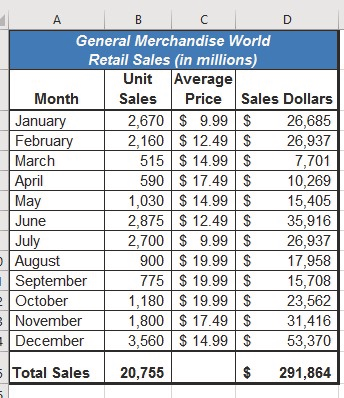
\includegraphics[width=\maxwidth{.95\linewidth}]{gfx/ch01_fig01}
	\caption{Example of an Excel Worksheet}
	\label{01:fig01}
\end{figure}

\subsection{Starting Excel}

\begin{enumerate}
	\item Locate Excel on the Windows menu.
	\item Click \fmtButton{Microsoft Excel} to launch the Excel application.
	\item Click the first option, \fmtButton{Blank Workbook}.
\end{enumerate}

\subsection{The Excel Workbook}

Once Excel is started, a blank workbook will open. A workbook is an Excel file that contains one or more worksheets (sometimes referred to as spreadsheets). Excel will assign a file name to the workbook, such as \textit{Book1}, \textit{Book2}, \textit{Book3}, and so on, depending on how many new workbooks are opened. Figure \ref{01:fig02} shows a blank workbook after starting Excel. Take some time to become familiar with this screen. (\textit{Note: the worksheet screen may be slightly different depending on the version of Excel being used.})

\begin{figure}[H]
	\centering
	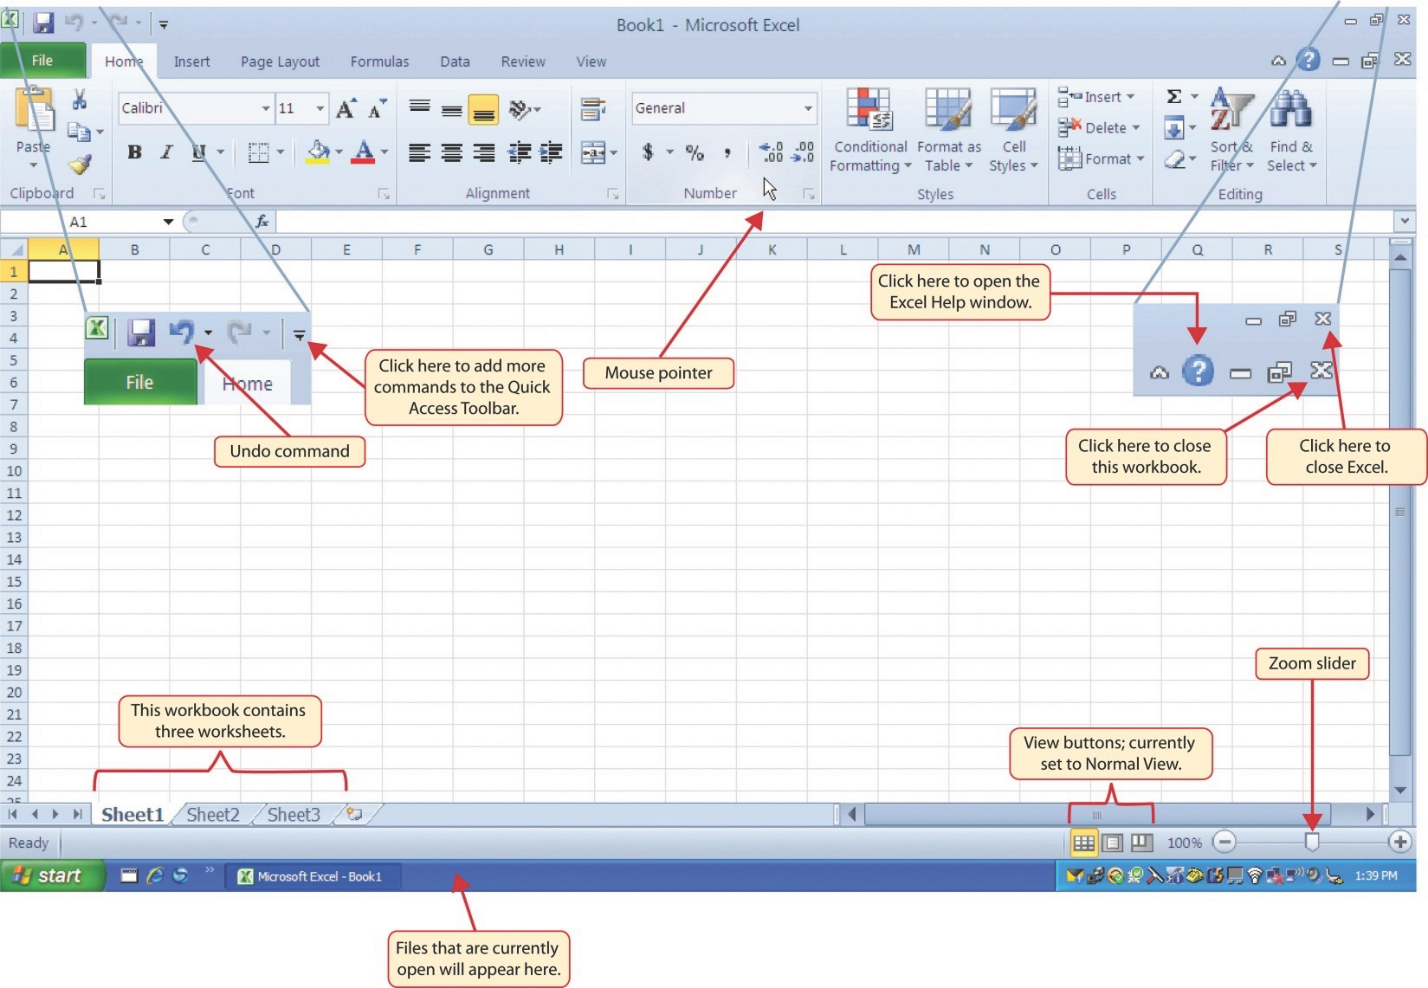
\includegraphics[width=\maxwidth{.95\linewidth}]{gfx/ch01_fig02}
	\caption{Blank Workbook}
	\label{01:fig02}
\end{figure}

The workbook should already be maximized (or shown at full size) once Excel is started, as shown in Figure \ref{01:fig02}. However, if the screen looks like Figure \ref{01:fig03} after starting Excel, click the \fmtButton{Maximize} button, as shown in the figure.

\begin{figure}[H]
	\centering
	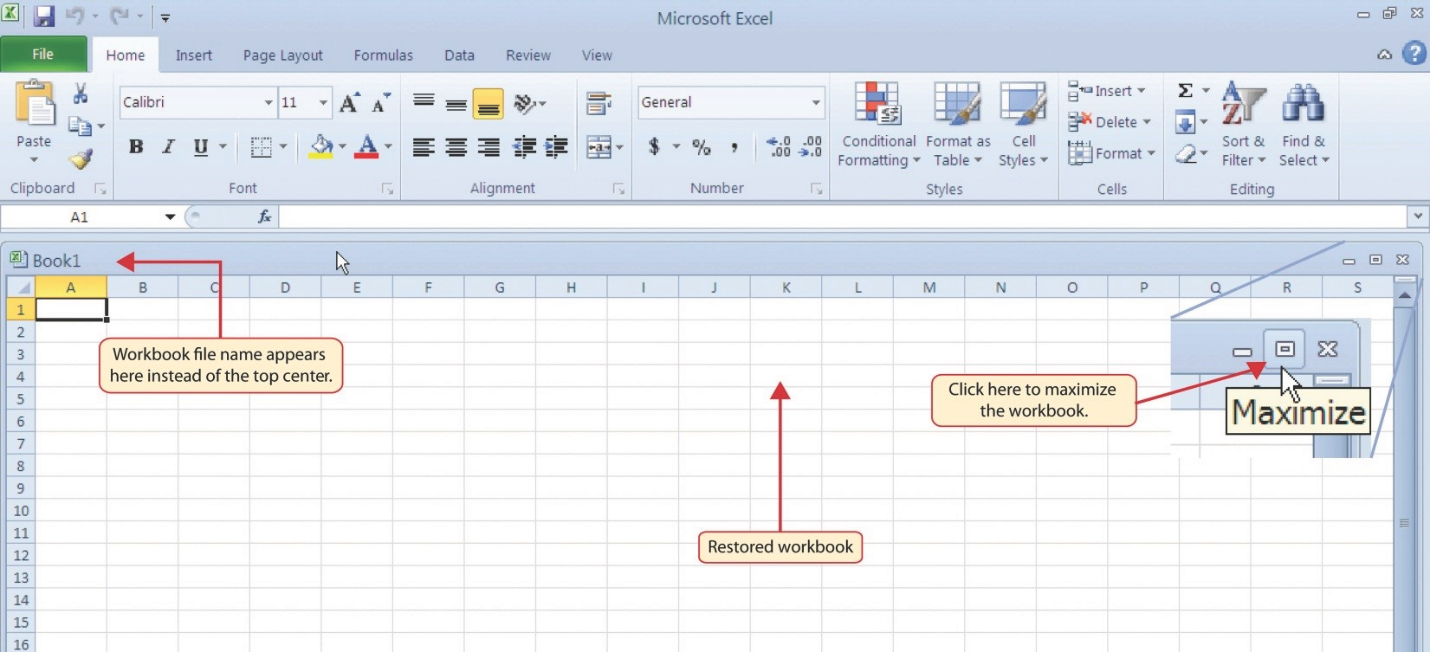
\includegraphics[width=\maxwidth{.95\linewidth}]{gfx/ch01_fig03}
	\caption{Restored Worksheet}
	\label{01:fig03}
\end{figure}

\subsection{Navigating Worksheets}

Data is entered and managed in an Excel worksheet. The worksheet contains several rectangles called cells for entering numeric and non-numeric data. Each cell in an Excel worksheet is located at an address, which is defined by a column letter followed by a row number. For example, the cell that is currently activated in Figure \ref{01:fig03} is $ A1 $. This would be referred to as cell location $ A1 $ or cell reference $ A1 $. The following steps explain how to navigate in an Excel worksheet.

\begin{itemize}
	\item Place the mouse pointer over cell \fmtLoc{D5} and left click.
	\item Check to make sure \fmtLoc{Column D} and \fmtLoc{Row 5} are highlighted, as shown in Figure \ref{01:fig04}.
\end{itemize}

\begin{figure}[H]
	\centering
	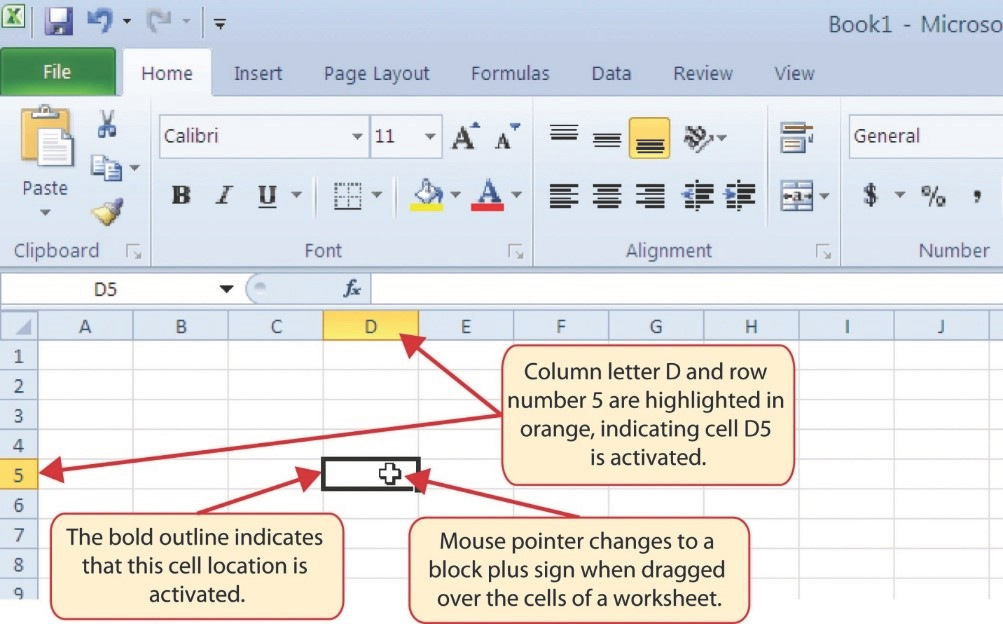
\includegraphics[width=\maxwidth{.95\linewidth}]{gfx/ch01_fig04}
	\caption{Activating a Cell Location}
	\label{01:fig04}
\end{figure}

\begin{enumerate}
	\item Click the mouse pointer in cell \fmtLoc{A1}.
	\item Click and hold the left mouse button and drag the mouse pointer back to cell \fmtLoc{D5}.
	\item Release the left mouse button. Several cells are now highlighted, as shown in Figure \ref{01:fig05}.
\end{enumerate}

\begin{figure}[H]
	\centering
	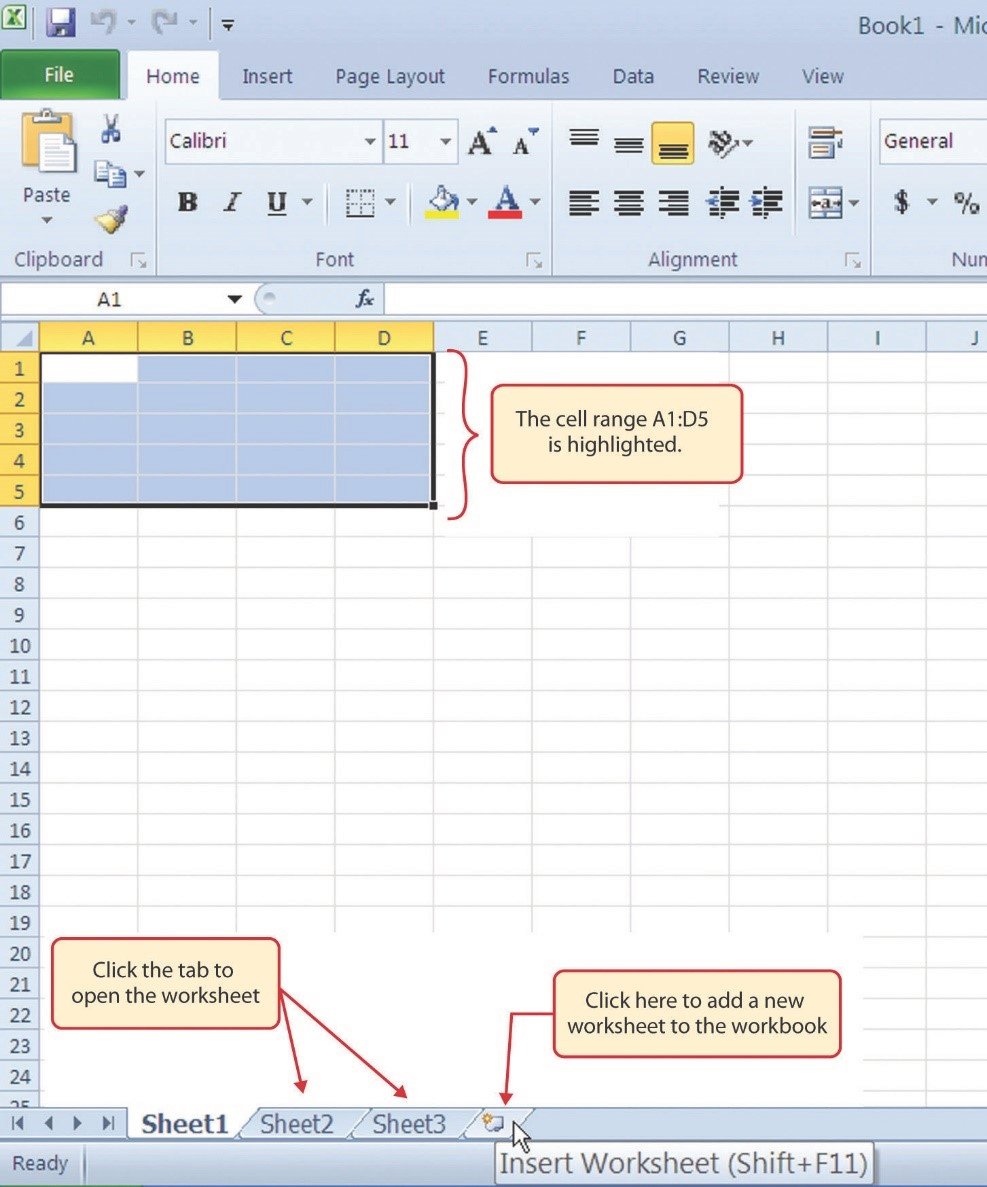
\includegraphics[width=\maxwidth{.95\linewidth}]{gfx/ch01_fig05}
	\caption{Highlighting a Range of Cells}
	\label{01:fig05}
\end{figure}

This is referred to as a cell range and is usually written as $ A1 $:$ D5 $. Any two cell locations separated by a colon are known as a cell range. The first cell in the range is the top left corner and the second cell is the lower right corner.

\begin{enumerate}
	\item At the bottom of the screen are tabs that identify different worksheets. Depending on the version of Excel being used there may be three as displayed in Figure \ref{01:fig05} or just one. If there is only one sheet, clicking \fmtButton{Insert Worksheet} adds a new worksheet. Different versions of Excel use \fmtButton{$ + $} or \fmtButton{Insert Worksheet} buttons. For this exercise, add worksheets as necessary so three are available.
	\item Click the \fmtWorksheet{Sheet1} tab at the bottom of the screen to activate it, as shown in Figure \ref{01:fig05}.
\end{enumerate}

\begin{center}
	\begin{shtcutbox}{Keyboard Shortcuts}
		\textbf{Basic Worksheet Navigation}
		\\
		\begin{itemize}
			\setlength{\itemsep}{0pt}
			\setlength{\parskip}{0pt}
			\setlength{\parsep}{0pt}

			\item Use the arrow keys on the keyboard to move the cell pointer to different cells on the worksheet.
			\item Hold the \fmtKeystroke{Shift} key and press the arrow keys on the keyboard to highlight a range of cells in a worksheet.
			\item Hold the \fmtKeystroke{Ctrl} key while pressing the \fmtKeystroke{Page Down} or \fmtKeystroke{Page Up} keys to open other worksheets in a workbook.

		\end{itemize}
	\end{shtcutbox}
\end{center}

\subsection{The Excel Ribbon}

Excel's features and commands are found in the \textit{Ribbon}, which is the upper area of the Excel screen that contains several tabs running across the top. Each tab provides access to a different set of Excel commands. Figure \ref{01:fig06} shows the commands available in the \textit{Home} tab of the Ribbon. Table \ref{01:tab01}, \textit{Command Overview for Each Tab of the Ribbon}, provides an overview of the commands that are found in each tab of the Ribbon.

\begin{figure}[H]
	\centering
	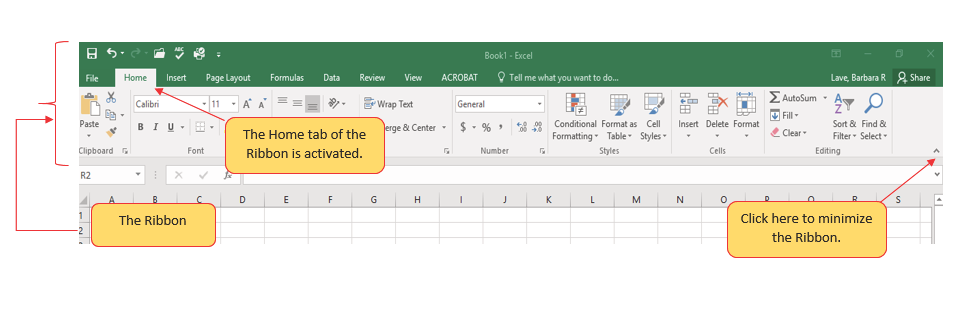
\includegraphics[width=\maxwidth{.95\linewidth}]{gfx/ch01_fig06}
	\caption{Home Tab of the Ribbon}
	\label{01:fig06}
\end{figure}

\begin{table}[H]
	\rowcolors{1}{}{tablerow} % zebra striping background
	{\small
		%\fontsize{8}{10} \selectfont %Replace small for special font size
		\begin{longtable}{L{0.75in}L{3.50in}} %Left-aligned, Max width: 4.25in
			\textbf{Tab} & \textbf{Description} \endhead
			\hline

			File & Also known as the \textit{Backstage View} of the Excel workbook. Contains all commands for opening, closing, saving, and creating new Excel workbooks. Includes print commands, document properties, e-mailing options, and help features. Excel's user options are also found in this tab.\\

			Home & Contains the most frequently used Excel commands. Formatting commands are found in this tab along with commands for cutting, copying, pasting, and for inserting and deleting rows and columns.\\
			
			Insert & Used to insert objects such as charts, pictures, shapes, PivotTables, Internet links, symbols, or text boxes.\\
			
			Page Layout & Contains commands used to prepare a worksheet for printing. Also includes commands used to show and print the grid lines on a worksheet.\\
			
			Formulas & Includes commands for adding mathematical functions to a worksheet. Also contains tools for auditing mathematical formulas.\\
			
			Data & Used when working with external data sources such as Microsoft® Access®, text files, or the Internet. Also contains sorting commands and access to scenario tools.\\
			
			Review & Includes Spelling and Track Changes features. Also contains protection features to password protect worksheets or workbooks.\\
			
			View & Used to adjust the visual appearance of a workbook. Common commands include the Zoom and Page Layout view.\\

			\rowcolor{captionwhite}
			\caption{Command Overview for Ribbon Tabs}
			\label{01:tab01}
		\end{longtable}
	} % End small
\end{table}

The Ribbon shown in Figure \ref{01:fig06} is full, or maximized. The benefit of having a full Ribbon is that the commands are always visible while developing a worksheet. However, depending on the screen dimensions of the computer, the Ribbon may take up too much vertical space on the worksheet. If this is the case, it can be minimized by clicking the button shown in Figure \ref{01:fig06}. When minimized, the Ribbon will show only the tabs and not the command buttons. Clicking a tab makes the command buttons appear until a command is selected or the mouse is clicked anywhere on the worksheet. Once the ribbon is expanded it can be pinned open by clicking the \fmtButton{pin} button at the lower left corner of the ribbon.

\begin{center}
	\begin{shtcutbox}{Keyboard Shortcuts}
		\textbf{Minimizing or Maximizing the Ribbon}
		\\
		\begin{itemize}
			\setlength{\itemsep}{0pt}
			\setlength{\parskip}{0pt}
			\setlength{\parsep}{0pt}
			
			\item Hold down the \fmtKeystroke{Ctrl} key and press the \fmtKeystroke{F1} key to toggle between the maximized and minimized view of the ribbon.
			
		\end{itemize}
	\end{shtcutbox}
\end{center}

\subsection{Quick Access Toolbar and Right-Click Menu}

The \textit{Quick Access Toolbar} is found at the upper left side of the Excel screen above the Ribbon, as shown in Figure \ref{01:fig07}. This area provides access to the most frequently used commands, such as Save and Undo. The \textit{Quick Access Toolbar} can be customized by adding commands that are regularly used. By placing these commands in the \textit{Quick Access Toolbar}, it is not necessary to navigate through the Ribbon to find them. To customize the \textit{Quick Access Toolbar}, click the down arrow as shown in Figure \ref{01:fig07}. This will open a menu of commonly-used commands that can be added to the \textit{Quick Access Toolbar}. If the desired command is not on the list, select the \textit{More Commands} option, which opens a screen containing every command on the ribbon.

\begin{figure}[H]
	\centering
	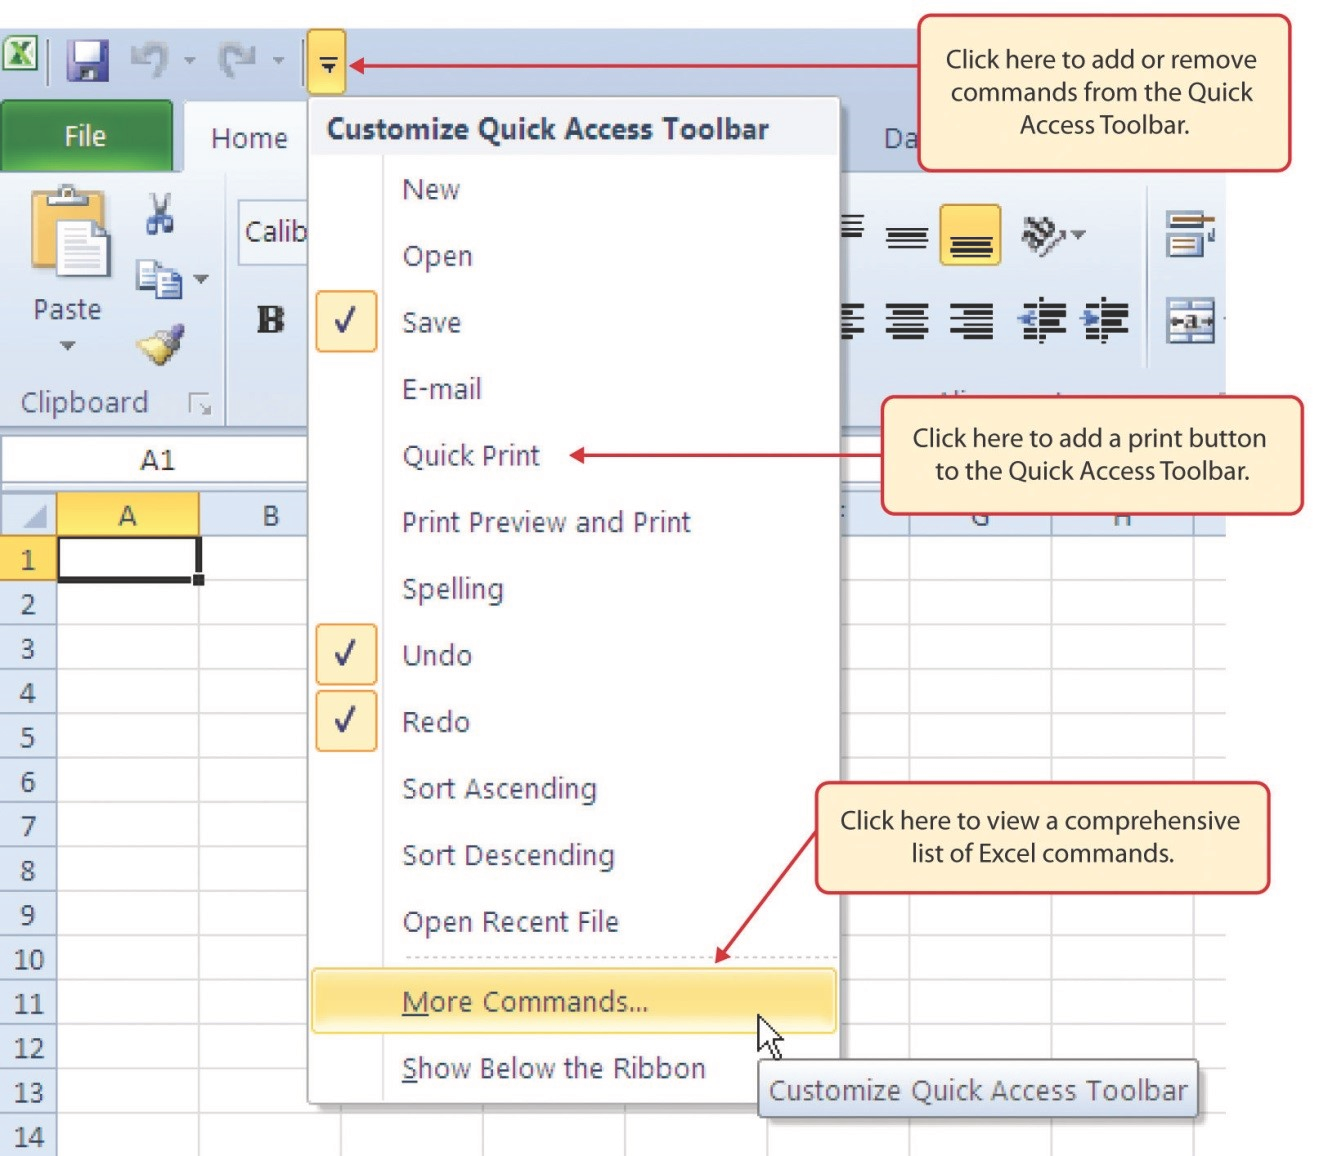
\includegraphics[width=\maxwidth{.95\linewidth}]{gfx/ch01_fig07}
	\caption{Customizing the Quick Access Toolbar}
	\label{01:fig07}
\end{figure}

In addition to the Ribbon and Quick Access Toolbar, commands can also be accessed by right-clicking anywhere on the worksheet and opening a context menu. \ref{01:fig08} shows an example of the commands available in the context menu.

\begin{figure}[H]
	\centering
	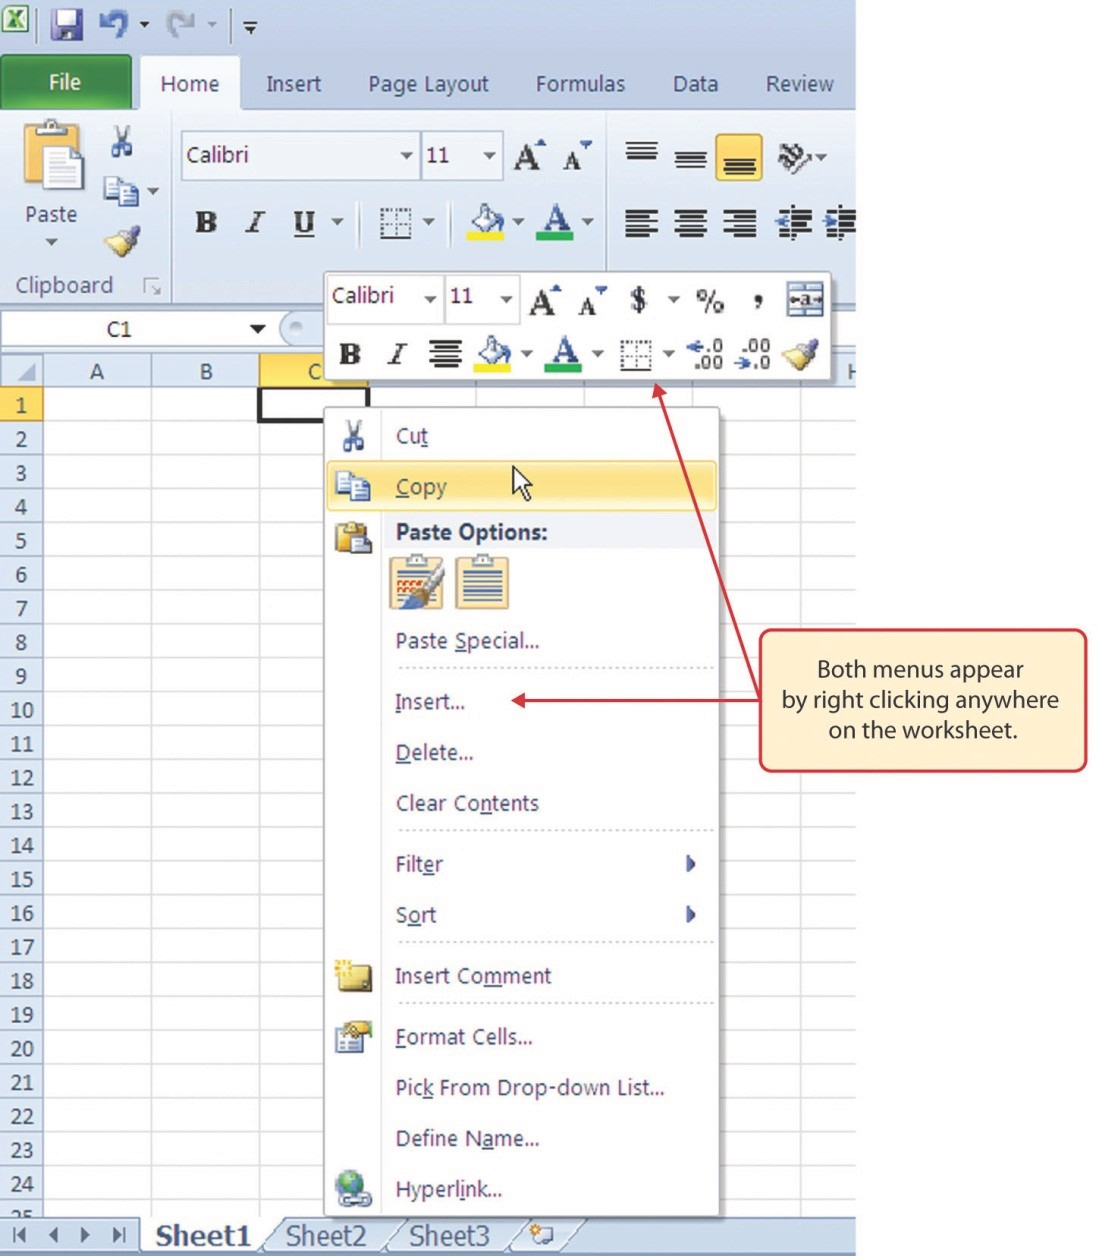
\includegraphics[width=\maxwidth{.95\linewidth}]{gfx/ch01_fig08}
	\caption{Right-Click Menu}
	\label{01:fig08}
\end{figure}

\subsection{The File Tab}

The \textit{File} tab is also known as the \textit{Backstage} view of the workbook. It contains a variety of features and commands related to the workbook that is currently open, new workbooks, or workbooks stored in other locations on the computer or network. Figure \ref{01:fig09} shows the options available in the \textit{File} tab or \textit{Backstage} view. To leave the \textit{Backstage} view and return to the worksheet, click the arrow in the upper left-hand corner as shown in Figure \ref{01:fig09}.

\begin{figure}[H]
	\centering
	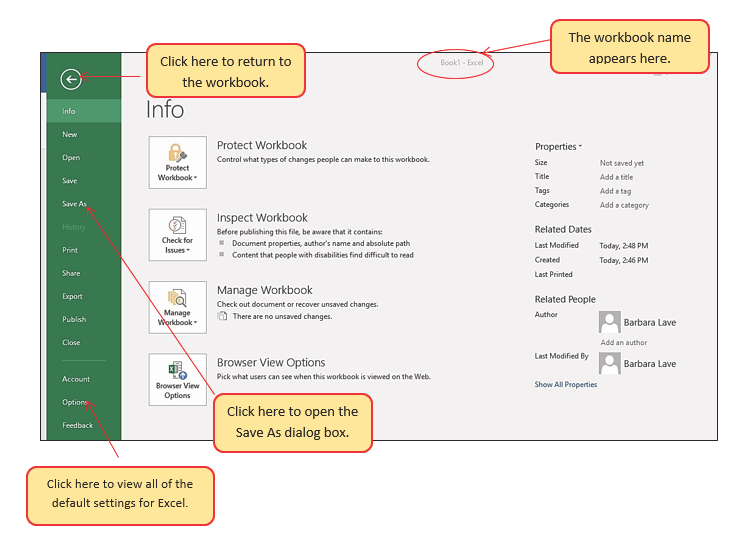
\includegraphics[width=\maxwidth{.95\linewidth}]{gfx/ch01_fig09}
	\caption{File Tab or Backstage View of a Workbook}
	\label{01:fig09}
\end{figure}

Included in the \textit{File} tab are the numerous Excel settings that can be accessed and modified by clicking the \textit{Options} button. Figure \ref{01:fig10} shows the Excel \textit{Options} window, which opens access to settings such as the default font style, font size, and the number of worksheets that appear in new workbooks\footnote{Chapter \ref{ch09:topics}, \nameref{ch09:topics}, page \pageref{ch09:topics}, has more information about setting common options.}.

\begin{figure}[H]
	\centering
	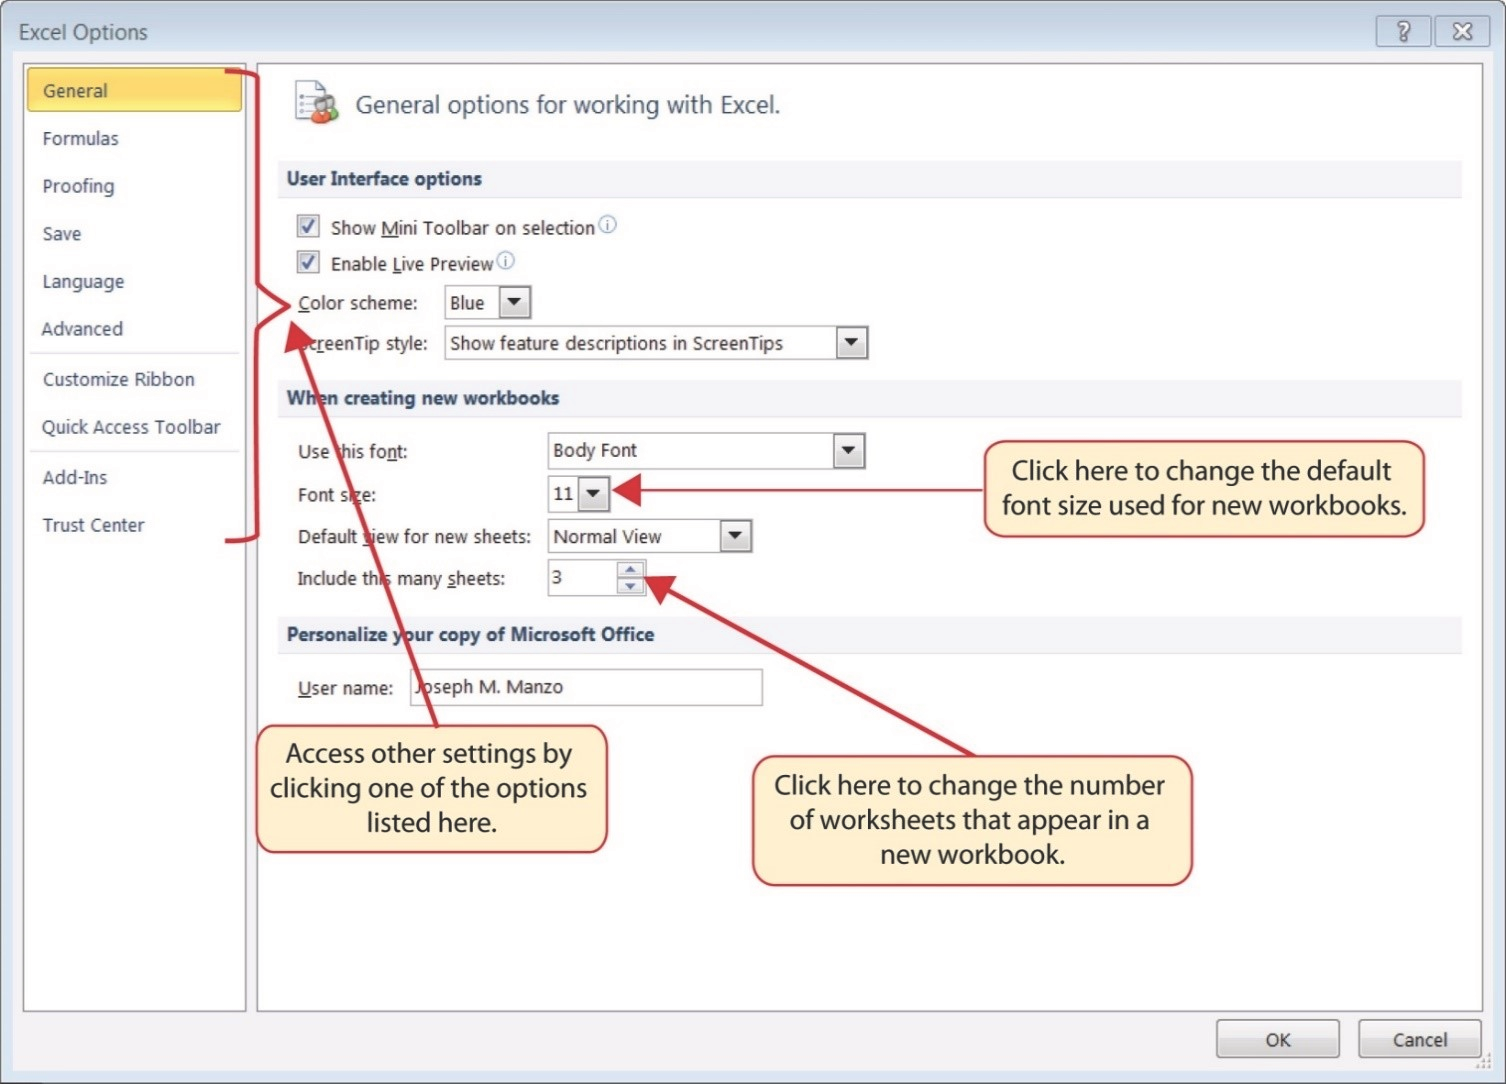
\includegraphics[width=\maxwidth{.95\linewidth}]{gfx/ch01_fig10}
	\caption{Excel Options Window}
	\label{01:fig10}
\end{figure}

\subsection{Saving Workbooks (Save As)}

Once a new workbook is created, the file name needs to be specified and a location chosen on the computer or network to save that file. A blank workbook was opened earlier in this lesson and it should now be saved. It is important to remember where the workbook is saved since it will be used later in this chapter to construct the workbook shown in Figure \ref{01:fig01}. As a tip, it is probably easiest to store all workbooks used in this course in the same folder.

\begin{enumerate}[resume]
	\item Click \fmtButton{File $ \Rightarrow $ Save As}. This will open the \textit{Save As} dialog.
	\item Determine a location for saving on the computer by clicking \fmtButton{Browse} on the left side to open the \textit{Save As} dialog box as illustrated in Figure \ref{01:fig12}.
	\item Click in the \textit{File Name} box near the bottom of the \textit{Save As} dialog box. Type the new file name: \fmtTyping{CH1-GMW Sales Data}
	\item Review the settings in the screen for correctness and click the \fmtButton{Save} button.
\end{enumerate}

\begin{figure}[H]
	\centering
	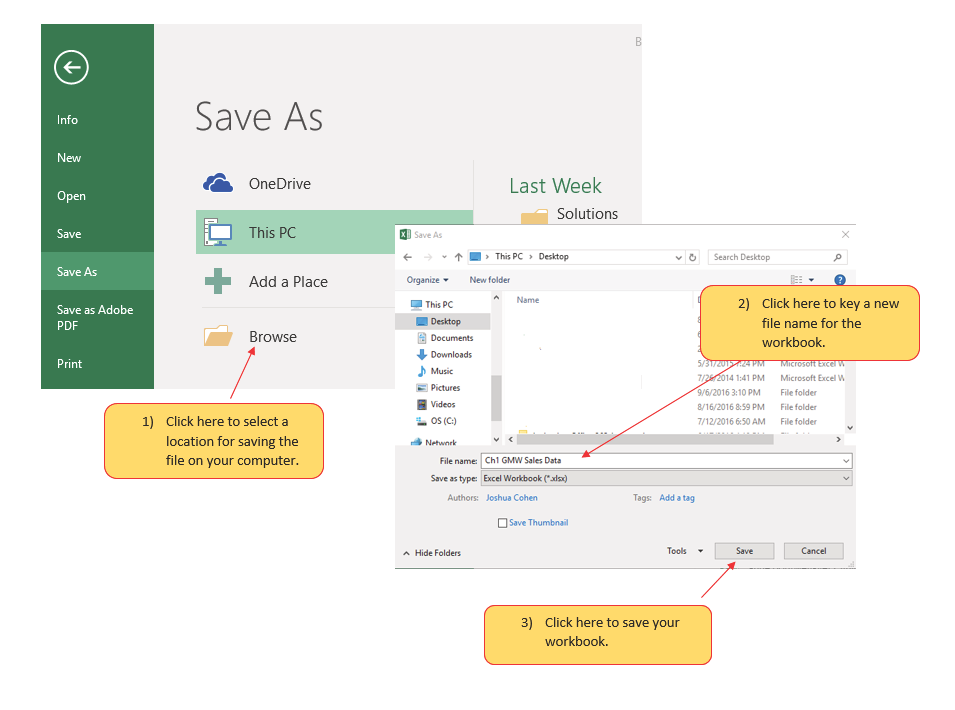
\includegraphics[width=\maxwidth{.95\linewidth}]{gfx/ch01_fig12}
	\caption{Save As Dialog in Excel}
	\label{01:fig12}
\end{figure}

\begin{center}
	\begin{shtcutbox}{Keyboard Shortcuts}
		\textbf{Save As}
		\\
		\begin{itemize}
			\setlength{\itemsep}{0pt}
			\setlength{\parskip}{0pt}
			\setlength{\parsep}{0pt}
			
			\item Press the \fmtKeystroke{F12} key and use the tab and arrow keys to navigate around the \textit{Save As} dialog box. Use the \fmtKeystroke{Enter} key to make a selection.
			\item Or press the \fmtKeystroke{Alt} key on the keyboard and Key Tips, small letters and numbers, appear on the Ribbon. Press the \fmtKeystroke{F} key on the keyboard for the \fmtButton{File} tab and then the \fmtKeystroke{A} key. This will open the \textit{Save As} dialog box.
			
		\end{itemize}
	\end{shtcutbox}
\end{center}

\begin{center}
	\begin{sklbox}{Skill Refresher}
		\textbf{Saving Workbooks (Save As)}
		\\
		\begin{itemize}
			\setlength{\itemsep}{0pt}
			\setlength{\parskip}{0pt}
			\setlength{\parsep}{0pt}
			
			\item Click the \textit{File} tab on the Ribbon.
			\item Click the \textit{Save As} option.
			\item Select a location on the computer.
			\item Click in the \textit{File} name box and type a new file name if needed.
			\item Click \textit{Save as type $ \Rightarrow $ Down Arrow} and select the appropriate file type if needed.
			\item Click the \textit{Save} button.
		
		\end{itemize}
	\end{sklbox}
\end{center}

\subsection{The Status Bar}

The Status Bar is located below the worksheet tabs on the Excel screen (see Figure \ref{01:fig13}). It displays a variety of information, such as the status of certain keys on the keyboard (\eg, CAPS LOCK), the available views for a workbook, the magnification of the screen, and mathematical functions that can be performed when data are highlighted on a worksheet. The Status Bar can be customized as follows.

\begin{enumerate}
	\item Place the mouse pointer over any area of the Status Bar and right-click to display the \textit{Customize Status Bar} list of options (see Figure \ref{01:fig13}).
	\item Select the \fmtButton{Caps Lock} option from the menu (see Figure \ref{01:fig13}).
	\item Press the \fmtKeystroke{Caps Lock} key on the keyboard and notice the Caps Lock indicator on the lower left side of the Status Bar.
	\item Press the \fmtKeystroke{Caps Lock} on the keyboard again. The indicator on the Status Bar goes away.
\end{enumerate}

\begin{figure}[H]
	\centering
	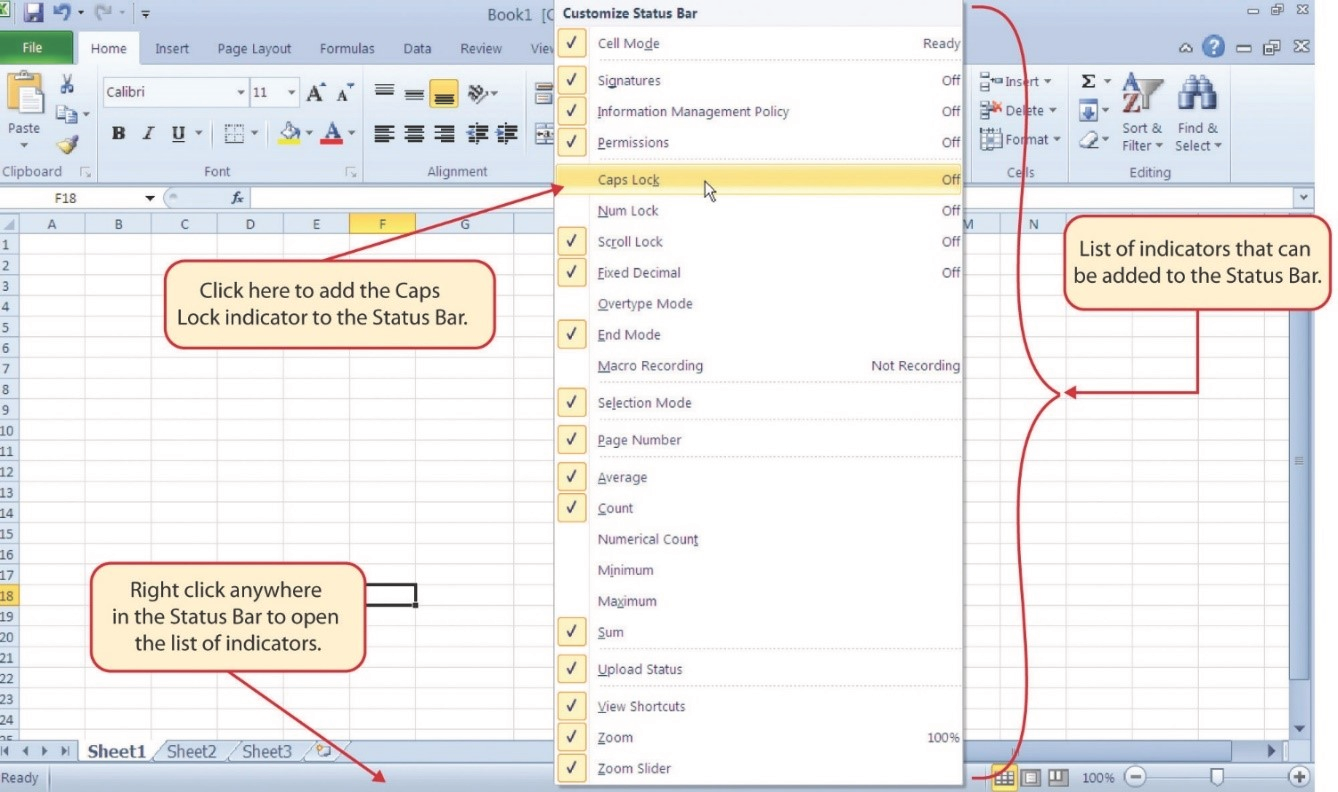
\includegraphics[width=\maxwidth{.95\linewidth}]{gfx/ch01_fig13}
	\caption{Customizing the Status Bar}
	\label{01:fig13}
\end{figure}

\subsection{Excel Help}

The Help feature provides extensive information about the Excel application. Although some of this information may be stored on the local computer, the Help window will automatically connect to the Internet if there is a live connection to provide resources that can answer most questions. 

\fmtOldExcel{Excel 2016} To access help, enter a question in the \textit{Tell me what you want to do} text box above the ribbon. A drop-down list with links to several potential answers will appear. Select from the links or click the question mark to launch the Excel Help window.

\fmtNewExcel{Excel 365} The Excel Help window can be opened by clicking the \fmtButton{Help} tab. Alternatively, enter a question in the \textit{Search} text box above the ribbon. A drop-down list with links to several potential answers will appear. Select from the links or click the question mark to launch the Excel Help window.

\begin{figure}[H]
	\centering
	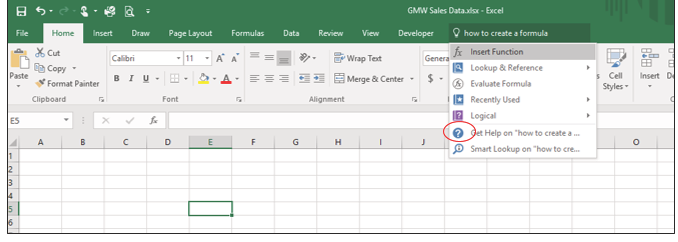
\includegraphics[width=\maxwidth{.95\linewidth}]{gfx/ch01_fig14}
	\caption{Excel Help Window}
	\label{01:fig14}
\end{figure}

\begin{center}
	\begin{shtcutbox}{Keyboard Shortcuts}
		\textbf{Excel Help}
		\\
		\begin{itemize}
			\setlength{\itemsep}{0pt}
			\setlength{\parskip}{0pt}
			\setlength{\parsep}{0pt}
			
			\item Press the \fmtKeystroke{F1} key on the keyboard.
			
		\end{itemize}
	\end{shtcutbox}
\end{center}


\begin{center}
	\begin{tkwbox}{Key Take-Aways}
		\textbf{Overview}
		\\
		\begin{itemize}
			\setlength{\itemsep}{0pt}
			\setlength{\parskip}{0pt}
			\setlength{\parsep}{0pt}
			
			\item Excel is a powerful tool for processing data for the purposes of making decisions.
			\item Excel commands are found throughout the tabs in the Ribbon.
			\item The \textit{Quick Access Toolbar} can be customized by adding frequently-used commands.
			\item Information displayed on the Status Bar can be customized.
			\item The Help window provides extensive information about Excel.
			
		\end{itemize}
	\end{tkwbox}
\end{center}

\section{Entering, Editing, and Managing Data}

\begin{center}
	\begin{objbox}{Learning Objectives}
		\begin{itemize}
			\setlength{\itemsep}{0pt}
			\setlength{\parskip}{0pt}
			\setlength{\parsep}{0pt}
			
			\item Understand how to enter data into a worksheet.
			\item Examine how to edit data in a worksheet.
			\item Examine how the Auto Fill Handle is used when entering data.
			\item Understand how to delete data from a worksheet and use the Undo command.
			\item Examine how to adjust column widths and row heights in a worksheet.
			\item Understand how to hide columns and rows in a worksheet.
			\item Examine how to insert columns and rows into a worksheet.
			\item Understand how to delete columns and rows from a worksheet.
			\item Learn how to move data to different locations in a worksheet.

		\end{itemize}
	\end{objbox}
\end{center}

This section begins the development of the workbook shown in Figure \ref{01:fig01}. The skills covered in this section are typically used in the early stages of developing one or more worksheets in a workbook.

\subsection{Entering Data}

Begin building the workbook shown in Figure \ref{01:fig01} by manually entering data into the worksheet. Begin by entering the column headings in \textit{Row 2}.

\begin{enumerate}
	\item Click cell location \fmtLoc{A2} on the worksheet.
	\item Type the word \fmtTyping{Month}.
	\item Press the \fmtKeystroke{Tab} key. This will enter the word into cell \fmtLoc{A2} and activate the next cell to the right.
	\item Type \fmtTyping{Unit Sales} and press the \fmtKeystroke{Tab} key.
	\item Repeat the above step for the words \fmtTyping{Average Price} and then again for \fmtTyping{Sales Dollars}.
\end{enumerate}

Figure \ref{01:fig15} shows how the worksheet should appear after the column headings have been entered into \textit{Row 2}. Notice that the word \textit{Price} in cell location $ C2 $ is not visible. This is because the column is too narrow to fit the entry. This will be corrected in the next section.

\begin{figure}[H]
	\centering
	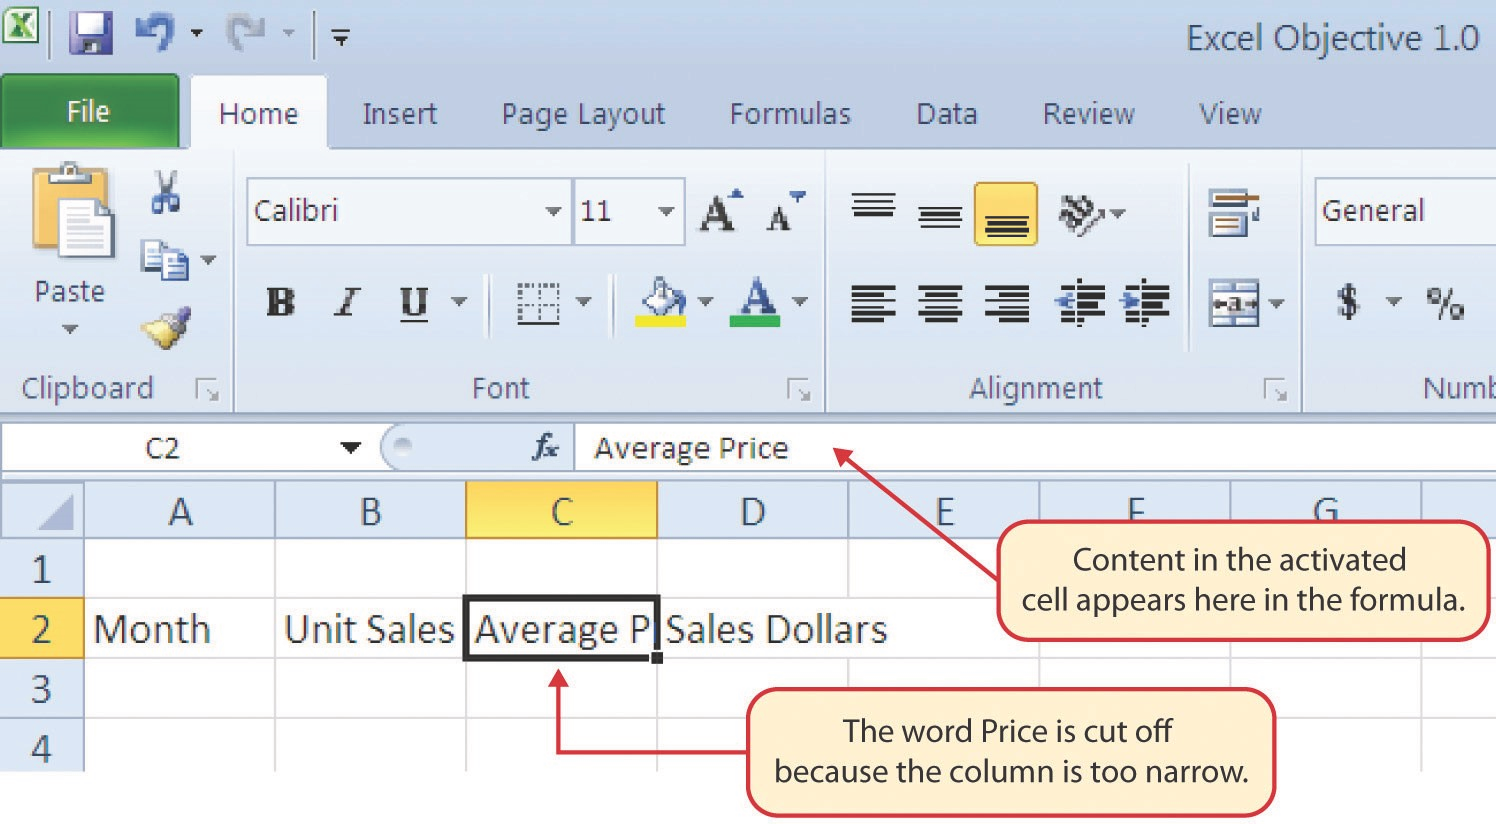
\includegraphics[width=\maxwidth{.95\linewidth}]{gfx/ch01_fig15}
	\caption{Entering Column Headings into a Worksheet}
	\label{01:fig15}
\end{figure}

\begin{center}
	\begin{infobox}{Integrity Check}
		\textbf{Column Headings}
		\\
		\\
		It is critical to include column headings that accurately describe the data in each column of a worksheet. In professional environments, Excel workbooks are commonly shared among coworkers. Good column headings reduce the chance of someone misinterpreting the data contained in a worksheet, which could lead to costly errors.
	\end{infobox}
\end{center}

\begin{enumerate}
	\item Click cell location \fmtLoc{B3}.
	\item Type the number \fmtTyping{$ 2670 $} and press the \fmtKeystroke{Enter} key. After pressing the \fmtKeystroke{Enter} key, cell \fmtLoc{B4} will be activated. Using the \fmtKeystroke{Enter} key is an efficient way to enter data vertically down a column.
	\item Enter the following numbers in cells \fmtLoc{B4} through \fmtLoc{B14}: \fmtTyping{$ 2160 $}, \fmtTyping{$ 515 $}, \fmtTyping{$ 590 $}, \fmtTyping{$ 1030 $}, \fmtTyping{$ $ 2875 $ $}, \fmtTyping{$ 2700 $}, \fmtTyping{$ 900 $}, \fmtTyping{$ 775 $}, \fmtTyping{$ 1180 $}, \fmtTyping{$ 1800 $}, and \fmtTyping{$ 3560 $}.
	\item Click cell location \fmtLoc{C3}.
	\item Type the number \fmtTyping{$ 9.99 $} and press the \fmtKeystroke{Enter} key.
	\item Enter the following numbers in cells \fmtLoc{C4} through \fmtLoc{C14}: \fmtTyping{$ 12.49 $}, \fmtTyping{$ 14.99 $}, \fmtTyping{$ 17.49 $}, \fmtTyping{$ 14.99 $}, \fmtTyping{$ 12.49 $}, \fmtTyping{$ 9.99 $}, \fmtTyping{$ 19.99 $}, \fmtTyping{$ 19.99 $}, \fmtTyping{$ 19.99 $}, \fmtTyping{$ 17.49 $}, and \fmtTyping{$ 14.99 $}.
	\item Click in cell \fmtLoc{D3}.
	\item Type the number \fmtTyping{$ 26685 $} and press the \fmtKeystroke{Enter} key.
	\item Enter the following numbers in cells \fmtLoc{D4} through \fmtLoc{D14}: \fmtTyping{$ 26937 $}, \fmtTyping{$ 7701 $}, \fmtTyping{$ 10269 $}, \fmtTyping{$ 15405 $}, \fmtTyping{$ 35916 $}, \fmtTyping{$ 26937 $}, \fmtTyping{$ 17958 $}, \fmtTyping{$ 15708 $}, \fmtTyping{$ 23562 $}, \fmtTyping{$ 31416 $}, and \fmtTyping{$ 53370 $}.
	\item When finished, check that the data entered matches Figure \ref{01:fig16}.
\end{enumerate}

\begin{figure}[H]
	\centering
	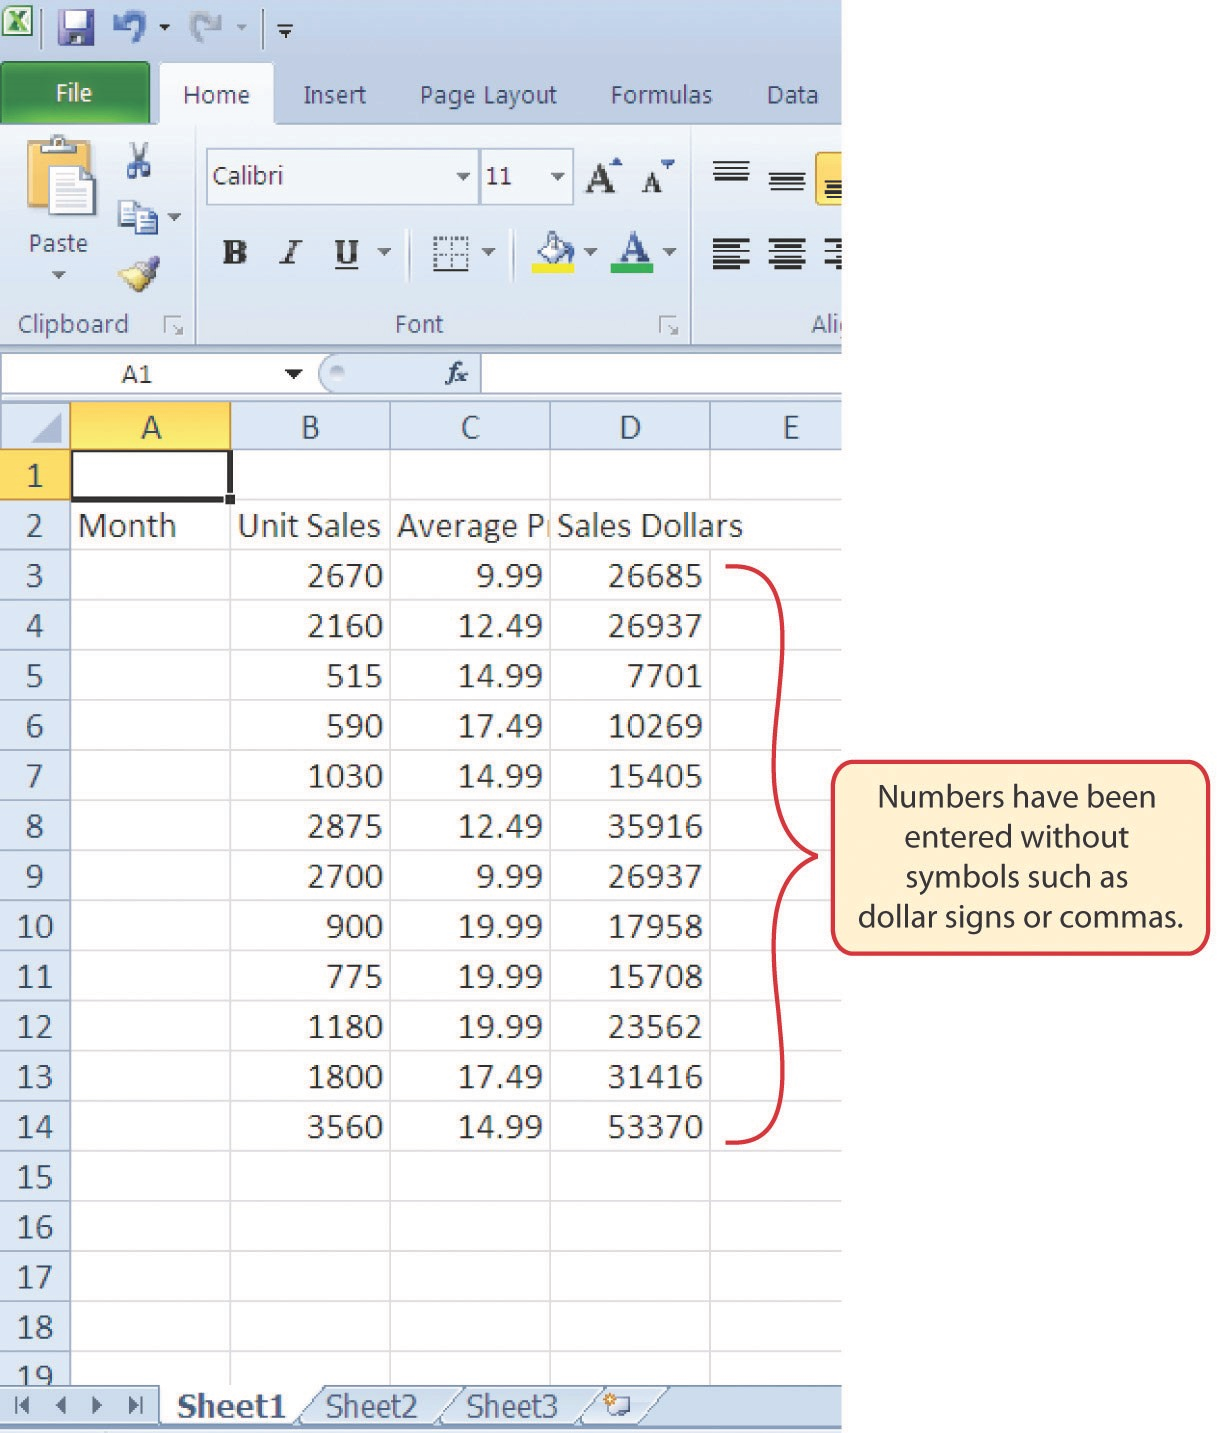
\includegraphics[width=\maxwidth{.95\linewidth}]{gfx/ch01_fig16}
	\caption{Completed Data Entry for Columns B, C, and D}
	\label{01:fig16}
\end{figure}

\begin{center}
	\begin{infobox}{Integrity Check}
		\textbf{Data Entry}
		\\
		\\
		One of the most likely points of error in any spreadsheet project is inaccurate data entry. When entering row and row of numbers it is easy to transpose or skip digits. Carefully checking data entry will reduce confusing results during the analysis phase of the project.
	\end{infobox}
\end{center}

\begin{center}
	\begin{infobox}{Why?}
		\textbf{Avoid Formatting Symbols When Entering Numbers}
		\\
		\\
		When typing numbers into an Excel worksheet, it is best to avoid adding any formatting symbols such as dollar signs and commas. Although Excel allows these symbols to be included while typing numbers, it slows down the process of entering data. It is more efficient to use Excel's formatting features to add these symbols to numbers after they are typed into a worksheet.
	\end{infobox}
\end{center}

\subsection{Editing Data}

Data that has been entered in a cell can be changed by double clicking the cell location or using the Formula Bar. The Formula Bar can be used for initial entery of data into cells as well as for editing data that already exists in a cell. The following steps provide an example of entering and then editing data that has been entered into a cell location.

\begin{enumerate}
	\item Click cell \fmtLoc{A15} in the \fmtWorksheet{Sheet1} worksheet.
	\item Type the abbreviation \fmtTyping{Tot} and press the \fmtKeystroke{Enter} key.
	\item Click cell \fmtLoc{A15}.
	\item Move the mouse pointer up to the Formula Bar. Notice that the pointer turns into a cursor. Move the cursor to the end of the abbreviation \textit{Tot} and left click.
	\item Type the letters \fmtTyping{al} to complete the word \textit{Total}.
	\item Click the checkmark to the left of the Formula Bar (see Figure \ref{01:fig17}) or press the \fmtKeystroke{Enter} key to enter the change into the cell.
\end{enumerate}

\begin{figure}[H]
	\centering
	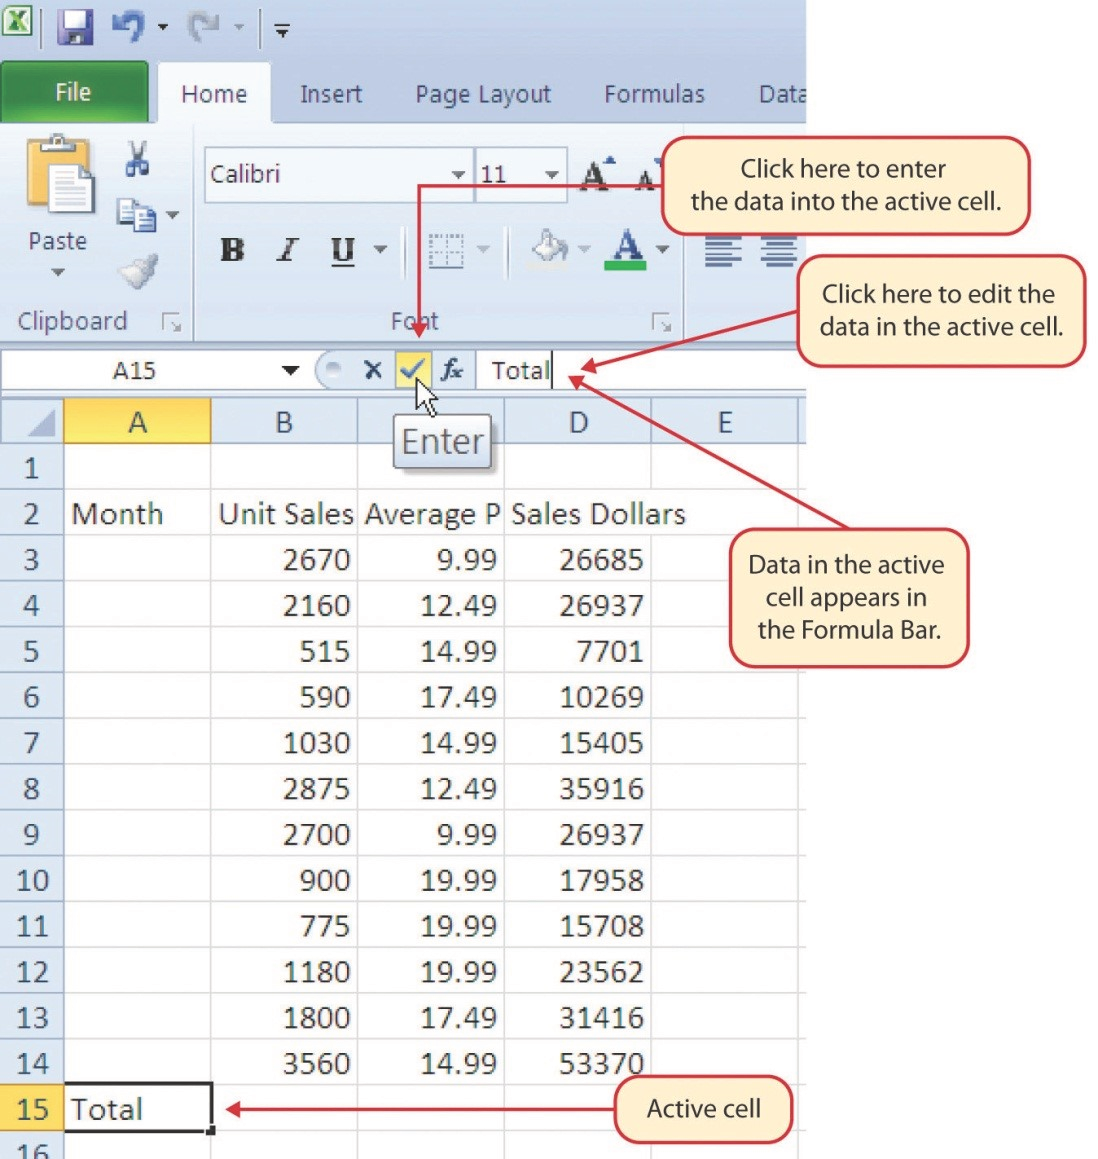
\includegraphics[width=\maxwidth{.95\linewidth}]{gfx/ch01_fig17}
	\caption{Using the Formula Bar to Edit and Enter Data}
	\label{01:fig17}
\end{figure}

\begin{enumerate}[resume]
	\item Double click cell \fmtLoc{A15}.
	\item Add a space after the word \textit{Total} and type the word \fmtTyping{Sales}.
	\item Press the \fmtKeystroke{Enter} key.
\end{enumerate}

\begin{center}
	\begin{shtcutbox}{Keyboard Shortcuts}
		\textbf{Editing Data in a Cell}
		\\
		\begin{itemize}
			\setlength{\itemsep}{0pt}
			\setlength{\parskip}{0pt}
			\setlength{\parsep}{0pt}
			
			\item Click in the cell that is to be edited and press the \fmtKeystroke{F2} key on the keyboard. Alternatively, double-click the cell to be edited.
			
		\end{itemize}
	\end{shtcutbox}
\end{center}

\subsection{Auto Fill}

The \textit{Auto Fill} feature is a valuable tool when manually entering data into a worksheet. This feature has many uses, but it is most beneficial when entering data in a defined sequence, such as the numbers $ 2 $, $ 4 $, $ 6 $, $ 8 $, and so on, or non-numeric data such as the days of the week or months of the year. The following steps demonstrate how the \textit{Auto Fill Handle} can be used to enter the months of the year in \textit{Column A}.

\begin{enumerate}
	\item Click cell \fmtLoc{A3} in the \fmtWorksheet{Sheet1} worksheet.
	\item Type the word \fmtTyping{January} and press the \fmtKeystroke{Enter} key.
	\item Click in cell \fmtLoc{A3} again.
	\item Move the mouse pointer to the lower right corner of cell \fmtLoc{A3}. Notice a small square in this corner of the cell which is called the \fmtButton{Auto Fill Handle} (See Figure \ref{01:fig18}) When the mouse pointer gets close to the \fmtButton{Auto Fill Handle}, the pointer's white block plus sign will turn into a black plus sign.
\end{enumerate}

\begin{figure}[H]
	\centering
	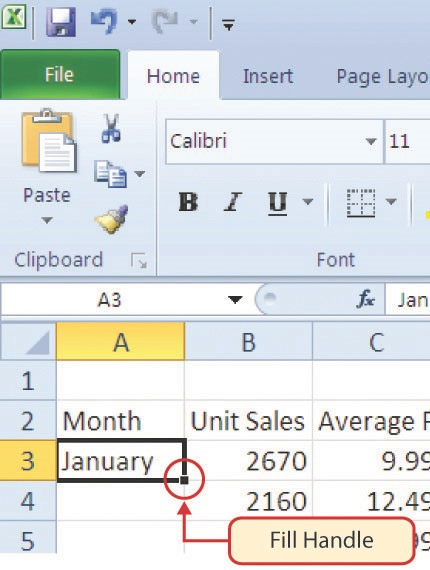
\includegraphics[width=\maxwidth{.95\linewidth}]{gfx/ch01_fig18}
	\caption{Auto Fill Handle}
	\label{01:fig18}
\end{figure}

\begin{enumerate}[resume]
	\item Left click and drag the \fmtButton{Auto Fill Handle} to cell \fmtLoc{A14}. Notice that the \fmtButton{Auto Fill Handle} tip box indicates what month will be placed into each cell (see Figure \ref{01:fig19}). Release the left mouse button when the tip box reads \textit{December}.
\end{enumerate}

\begin{figure}[H]
	\centering
	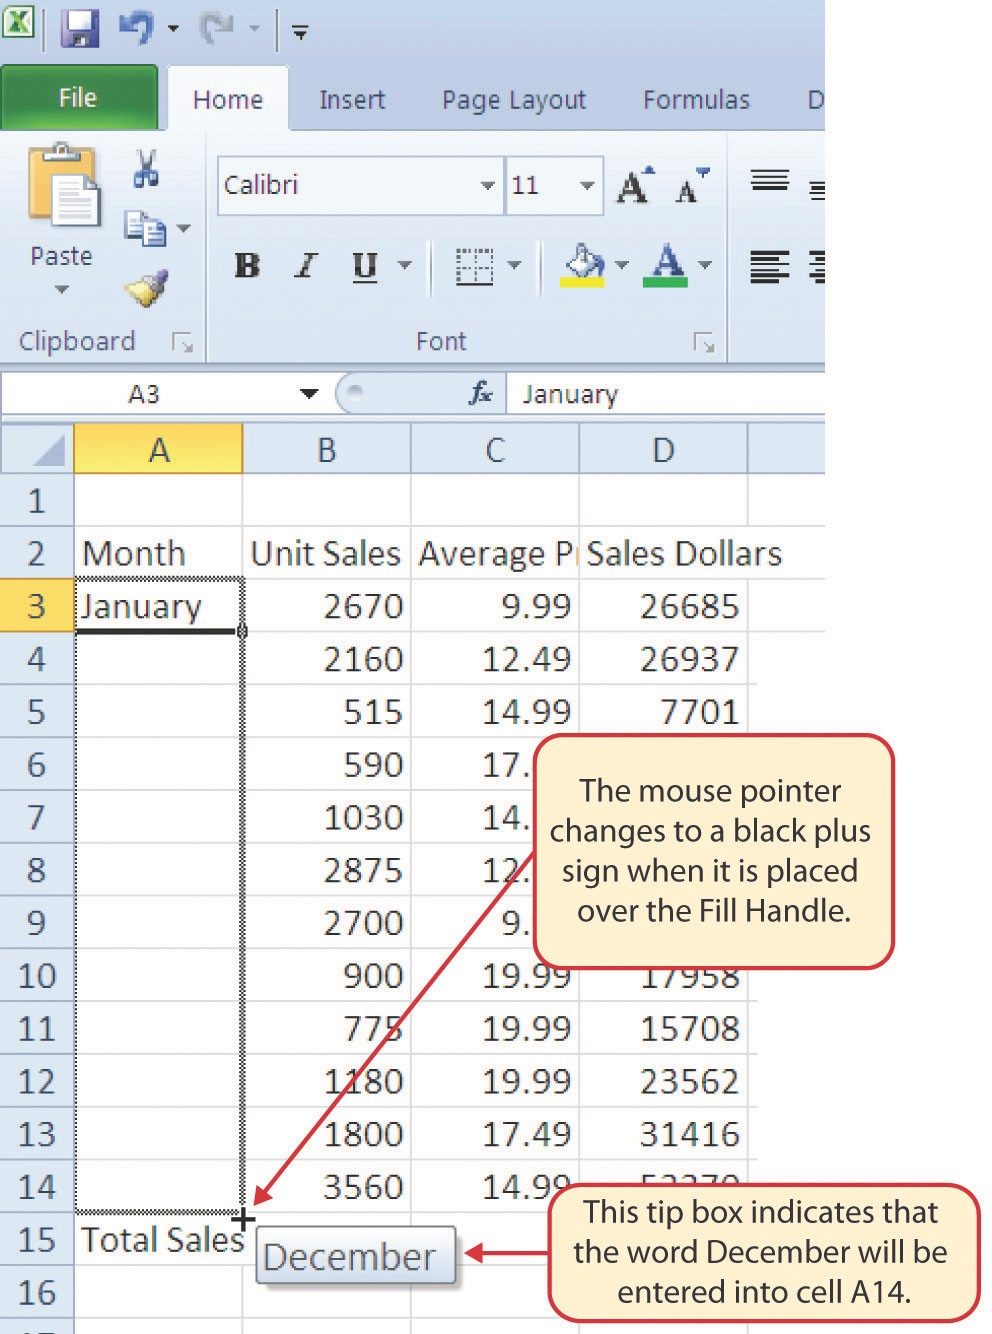
\includegraphics[width=\maxwidth{.95\linewidth}]{gfx/ch01_fig19}
	\caption{Using Auto Fill Handle to Enter the Months of the Year}
	\label{01:fig19}
\end{figure}

Once the left mouse button is released, all twelve months of the year should appear in the cell range $ A3 $:$ A14 $, as shown in Figure \ref{01:fig20}. After auto-filling a range, an \textit{Auto Fill Options} button pops up at the lower left corner of the filled range, as shown in Figure \ref{01:fig20}. 

\fmtOldExcel{Excel 2016} The \textit{Auto Fill Options} button presents several options for changing the way that the range is filled.

\begin{figure}[H]
	\centering
	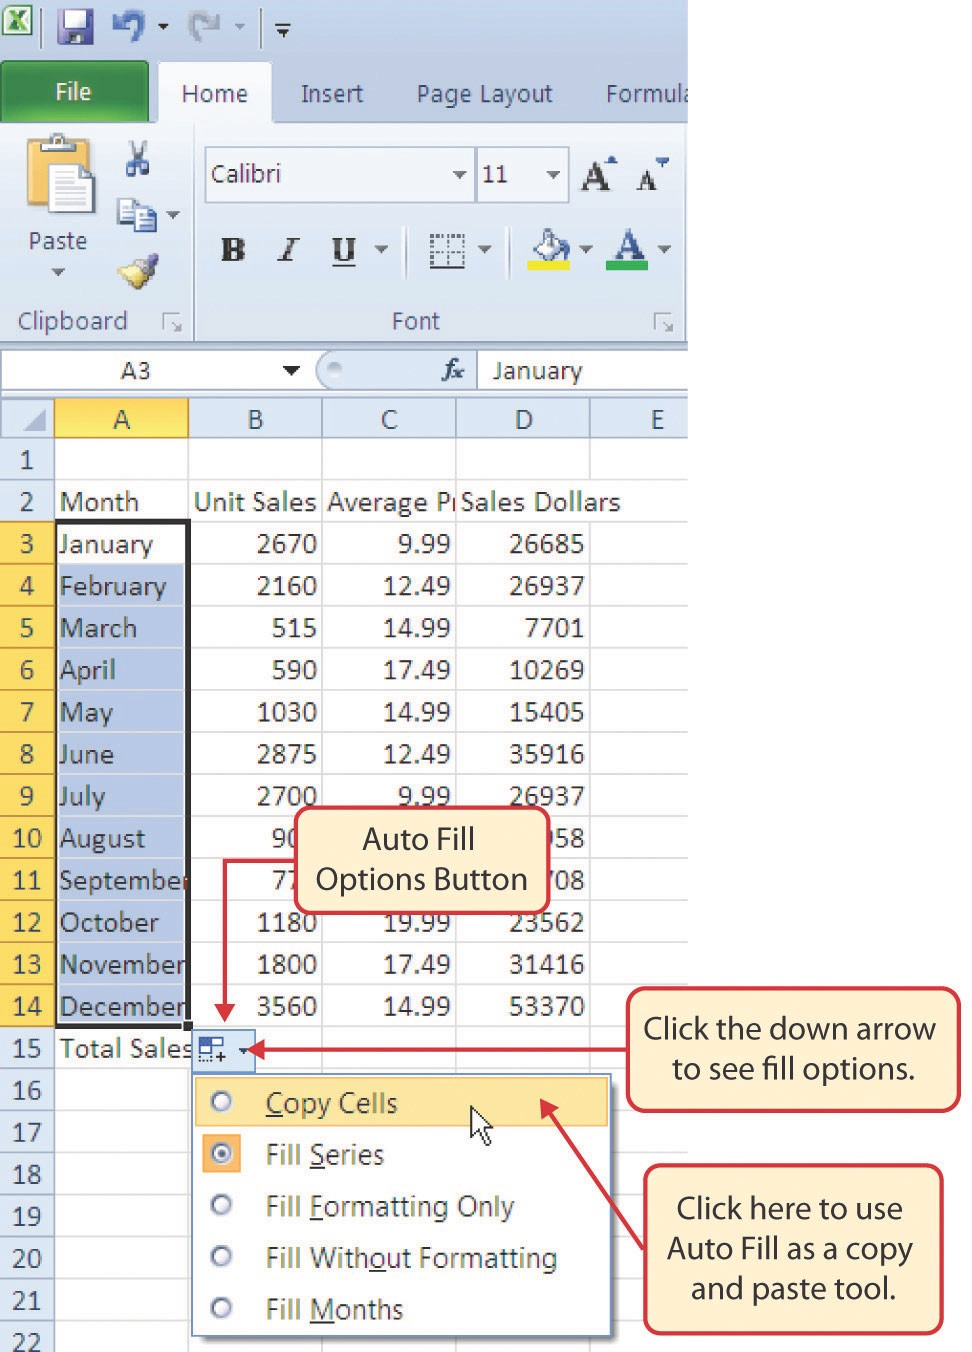
\includegraphics[width=\maxwidth{.95\linewidth}]{gfx/ch01_fig20}
	\caption{Auto Fill Options Button}
	\label{01:fig20}
\end{figure}

\begin{enumerate}
	\item Click the \fmtButton{Auto Fill Options} button.
	\item Click the \fmtButton{Copy Cells} option. This will change the months in the range \fmtLoc{A4:A14} to January.
	\item Click the \fmtButton{Auto Fill Options} button again.
	\item Click the \fmtButton{Fill Months} option to return the months of the year to the cell range \fmtLoc{A4:A14}. The \fmtButton{Fill Series} option will provide the same result.
\end{enumerate}

\fmtNewExcel{Excel 365} The \textit{Auto Fill Options} button was replaced with the \textit{Quick Analysis} button. That button will apply several possible analysis features to the filled range, like highlighting entries that are duplicates.

\begin{figure}[H]
	\centering
	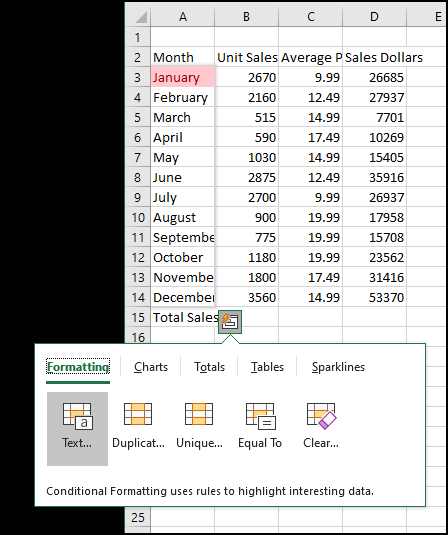
\includegraphics[width=\maxwidth{.95\linewidth}]{gfx/ch01_fig20a}
	\caption{Quick Analysis Button}
	\label{01:fig20a}
\end{figure}

\begin{enumerate}
	\item Click the \fmtButton{Quick Analysis} button.
	\item Hover the mouse over each of the Format tab options and notice how the text in the cells is highlighted.
	\item Click anywhere in the worksheet to finish the auto fill process.
\end{enumerate}

\subsection{Deleting Data and the Undo Command}

There are several methods for removing data from a worksheet, a few of which are demonstrated here. With each method, use the \textit{Undo} command to return the data that was deleted. Undo is available on the Quick Access Toolbar or use the keyboard shortcut of \fmtKeystroke{Ctrl} $ + $ \fmtKeystroke{Z}.This is a helpful command in the event that data is mistakenly deleted from the worksheet. The following steps demonstrate how to delete data from a cell or range of cells.

\begin{enumerate}
	\item Click cell \fmtLoc{C2} by placing the mouse pointer over the cell and clicking the left mouse button.
	\item Press the \fmtKeystroke{Delete} key on the keyboard. This removes the contents of the cell.
	\item Highlight the range \fmtLoc{C3:C14} by placing the mouse pointer over cell \fmtLoc{C3} then left click and drag the mouse pointer down to cell \fmtLoc{C14}.
	\item Place the mouse pointer over the \fmtButton{Auto Fill Handle}. Notice that the white block plus sign change to a black plus sign.
	\item Click and drag the mouse pointer up to cell \fmtLoc{C3}, as in Figure \ref{01:fig21}. Release the mouse button. The contents in the range \fmtLoc{C3:C14} will be removed.
\end{enumerate}

\begin{figure}[H]
	\centering
	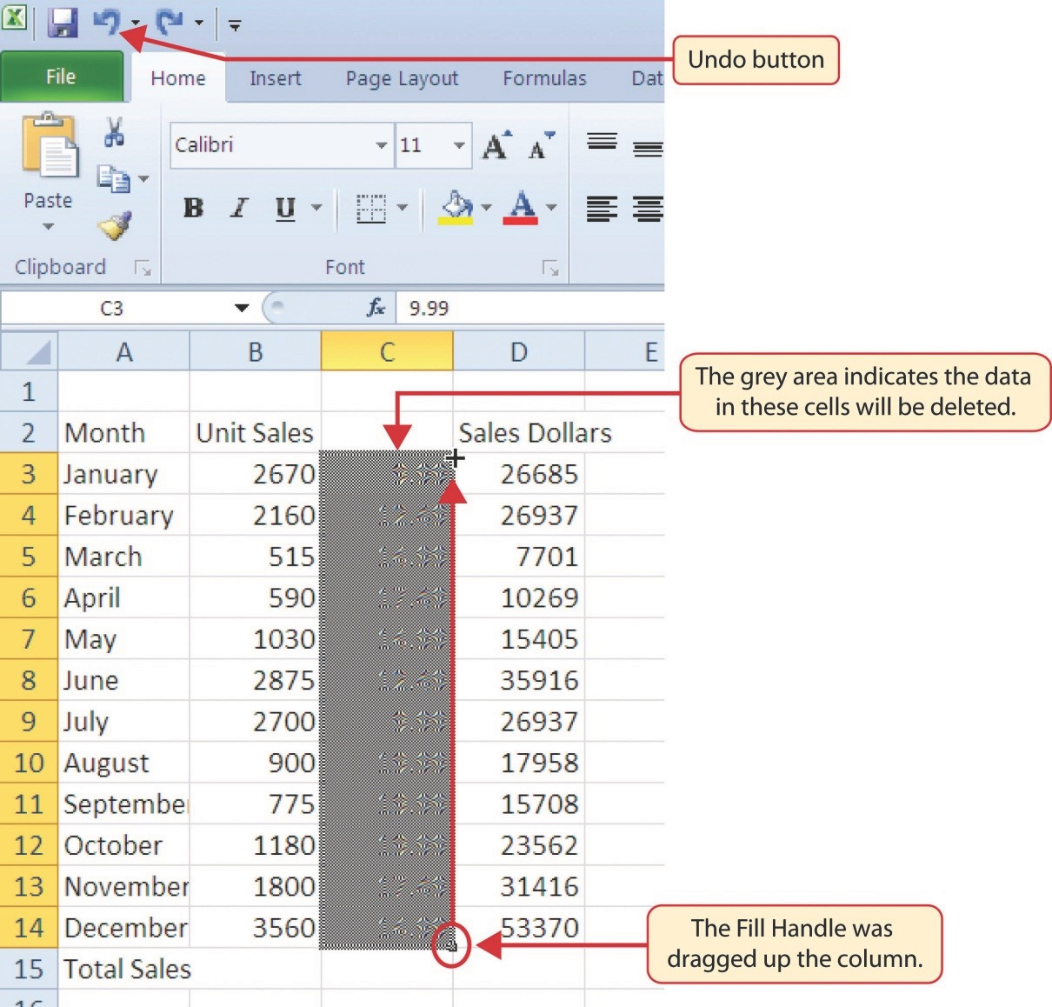
\includegraphics[width=\maxwidth{.95\linewidth}]{gfx/ch01_fig21}
	\caption{Using Auto Fill to Delete Contents of Cell}
	\label{01:fig21}
\end{figure}

\begin{enumerate}
	\item Click the \fmtButton{Undo} button in the \fmtButton{Quick Access Toolbar}, as illustrated in Figure \ref{01:fig21}. This should replace the data in the range \fmtLoc{C3:C14}.
	\item Click the \fmtButton{Undo} button again to replace the data in cell \fmtLoc{C2}.
\end{enumerate}

\begin{center}
	\begin{shtcutbox}{Keyboard Shortcuts}
		\textbf{Undo Command}
		\\
		\begin{itemize}
			\setlength{\itemsep}{0pt}
			\setlength{\parskip}{0pt}
			\setlength{\parsep}{0pt}
			
			\item Hold down the \fmtKeystroke{Ctrl} key while pressing the letter \fmtKeystroke{Z} on the keyboard.
			
		\end{itemize}
	\end{shtcutbox}
\end{center}

\begin{enumerate}[resume]
	\item Highlight the range \fmtLoc{C2:C14} by placing the mouse pointer over cell \fmtLoc{C2}. Then left click and drag the mouse pointer down to cell \fmtLoc{C14}.
	\item Click \fmtButton{Home $ \Rightarrow $ Editing $ \Rightarrow $ Clear} (see Figure \ref{01:fig22}). This opens a drop-down menu that contains several options for removing or clearing data from a cell. Notice that there are also options for clearing just the formats or the hyperlinks in a cell.
	\item Click the \fmtButton{Clear All} option. This removes the data in the cell range.
	\item Click the \fmtButton{Undo} button. This replaces the data in the range \fmtLoc{C2:C14}.
\end{enumerate}

\begin{figure}[H]
	\centering
	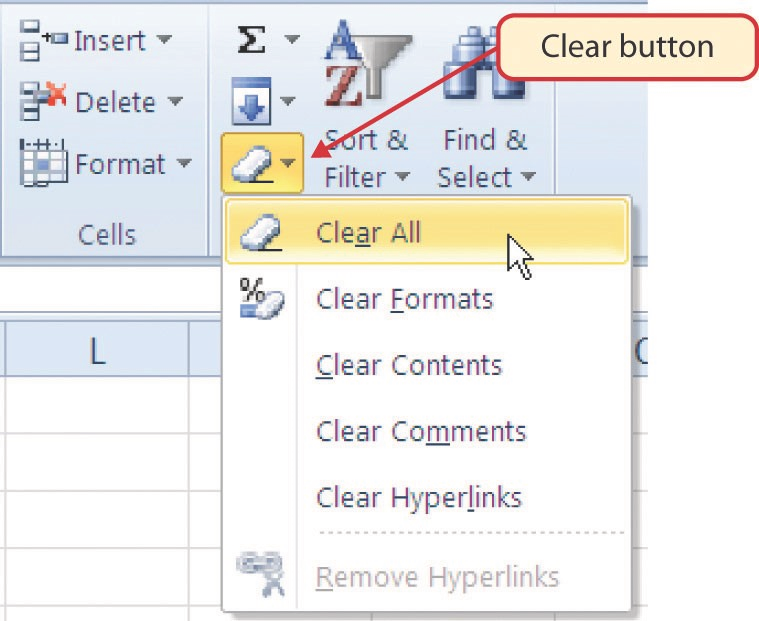
\includegraphics[width=\maxwidth{.95\linewidth}]{gfx/ch01_fig22}
	\caption{Clear Command Drop-Down Menu}
	\label{01:fig22}
\end{figure}

\subsection{Adjusting Columns and Rows}

There are a few entries in the worksheet that appear to be cut off. For example, the last letter of the word \textit{September} cannot be seen in cell $ A11 $. This is because the column is too narrow for this word. The columns and rows on an Excel worksheet can be adjusted to accommodate the data that is being entered into a cell. The following steps explain how to adjust the column widths and row heights in a worksheet.

\begin{enumerate}
	\item Bring the mouse pointer between \fmtLoc{Column A} and \fmtLoc{Column B} in the \fmtWorksheet{Sheet1} worksheet, as shown in Figure \ref{01:fig23}. Notice that the pointer's white block plus sign turns into double arrows.
	\item Click and drag the column to the right so the entire word \textit{September} in cell \fmtLoc{A11} can be seen. As the column separator is dragged to the right the column width pops up in a tip box. This box displays the number of characters that will fit into the column using the Calibri 11-point font which is the default setting for font/size.
	\item Release the left mouse button.
\end{enumerate}

\begin{figure}[H]
	\centering
	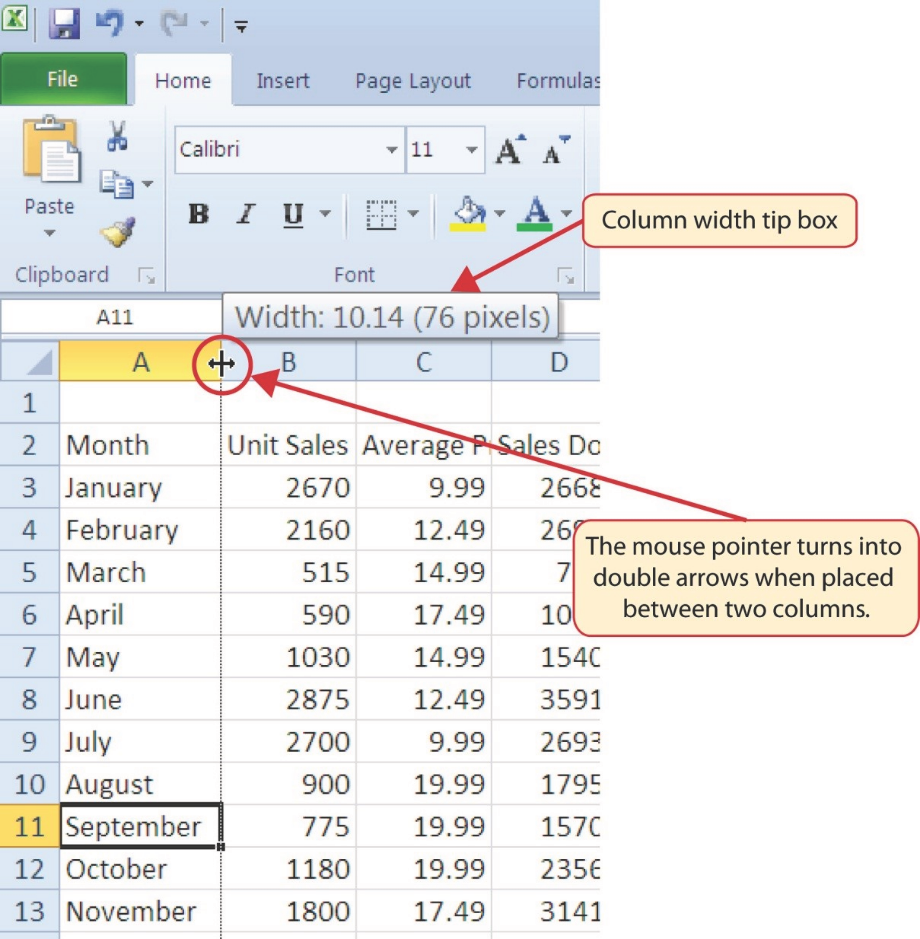
\includegraphics[width=\maxwidth{.95\linewidth}]{gfx/ch01_fig23}
	\caption{Adjusting Column Widths}
	\label{01:fig23}
\end{figure}

The click-and-drag method can be inefficient to set a specific character width for more than one column. The following steps illustrate a second method for adjusting columns to a specific width.

\begin{enumerate}
	\item Click any cell location in \fmtLoc{Column A} by moving the mouse pointer over a cell location and clicking the left mouse button. 
	\item Click \fmtButton{Home $ \Rightarrow $ Cells $ \Rightarrow $ Format $ \Rightarrow $ Column Width}. This will open the \textit{Column Width} dialog box.
	\item Type the number \fmtTyping{13} and click the \fmtButton{OK} button on the \textit{Column Width} dialog box. This will set \fmtLoc{Column A} to this character width (see Figure \ref{01:fig24}).
	\item As a third option, bring the mouse pointer between \fmtLoc{Column A} and \fmtLoc{Column B} so that the double arrow pointer displays and then double-click. This activates \fmtButton{AutoFit}, which adjusts the column width based on the longest entry in the column.
	\item Use the \textit{Column Width} dialog box to set the width to \fmtTyping{13}.
\end{enumerate}

\begin{figure}[H]
	\centering
	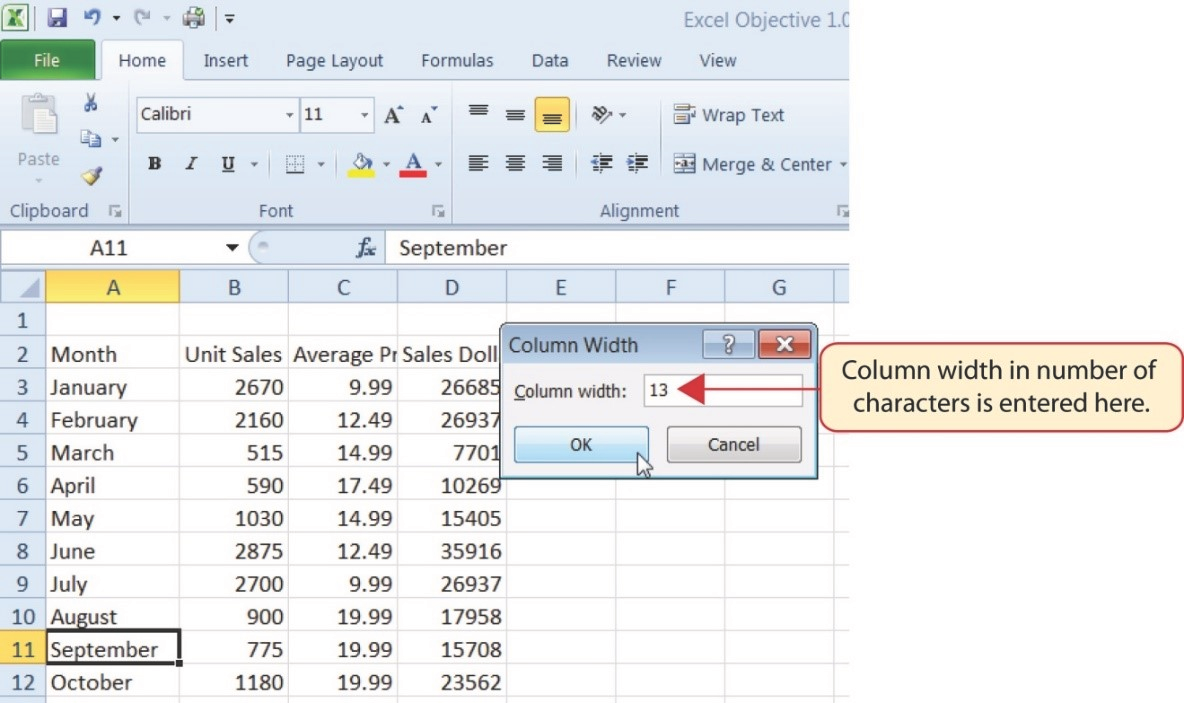
\includegraphics[width=\maxwidth{.95\linewidth}]{gfx/ch01_fig24}
	\caption{Column Width Dialog Box}
	\label{01:fig24}
\end{figure}

\begin{center}
	\begin{shtcutbox}{Keyboard Shortcuts}
		\textbf{Column Width}
		\\
		\begin{itemize}
			\setlength{\itemsep}{0pt}
			\setlength{\parskip}{0pt}
			\setlength{\parsep}{0pt}
			
			\item Press and release the \fmtKeystroke{Alt} key on the keyboard and then press the letters \fmtKeystroke{H}, \fmtKeystroke{O}, and \fmtKeystroke{W} one at a time.
			
		\end{itemize}
	\end{shtcutbox}
\end{center}

The following steps demonstrate how to adjust row height, which is similar to adjusting column width.

\begin{enumerate}
	\item Click cell \fmtLoc{A15}.
	\item Click \fmtButton{Home $ \Rightarrow $ Cells $ \Rightarrow $ Format $ \Rightarrow $ Row Height}. This will open the \textit{Row Height} dialog box.
	\item Type the number \fmtTyping{24} and click the \fmtButton{OK} button on the \textit{Row Height} dialog box. This will set \fmtLoc{Row $ 15 $} to a height of $ 24 $ points. A point is equivalent to approximately $ 1/72 $ of an inch. This adjustment in row height was made to create space between the totals for this worksheet and the rest of the data.
	\item Row height can also be adjusted by dragging the border between \fmtLoc{Row 15} and \fmtLoc{Row 16} or by double-clicking the border between \fmtLoc{Row 15} and \fmtLoc{Row 16}.
\end{enumerate}

\begin{center}
	\begin{shtcutbox}{Keyboard Shortcuts}
		\textbf{Column Width}
		\\
		\begin{itemize}
			\setlength{\itemsep}{0pt}
			\setlength{\parskip}{0pt}
			\setlength{\parsep}{0pt}
			
			\item Press the \fmtKeystroke{Alt} key on the keyboard, then press the letters \fmtKeystroke{H}, \fmtKeystroke{O}, and \fmtKeystroke{H} one at a time.
			
		\end{itemize}
	\end{shtcutbox}
\end{center}

Figure \ref{01:fig25} shows the appearance of the worksheet after \fmtLoc{Column A} and \fmtLoc{Row $ 15 $} are adjusted.

\begin{figure}[H]
	\centering
	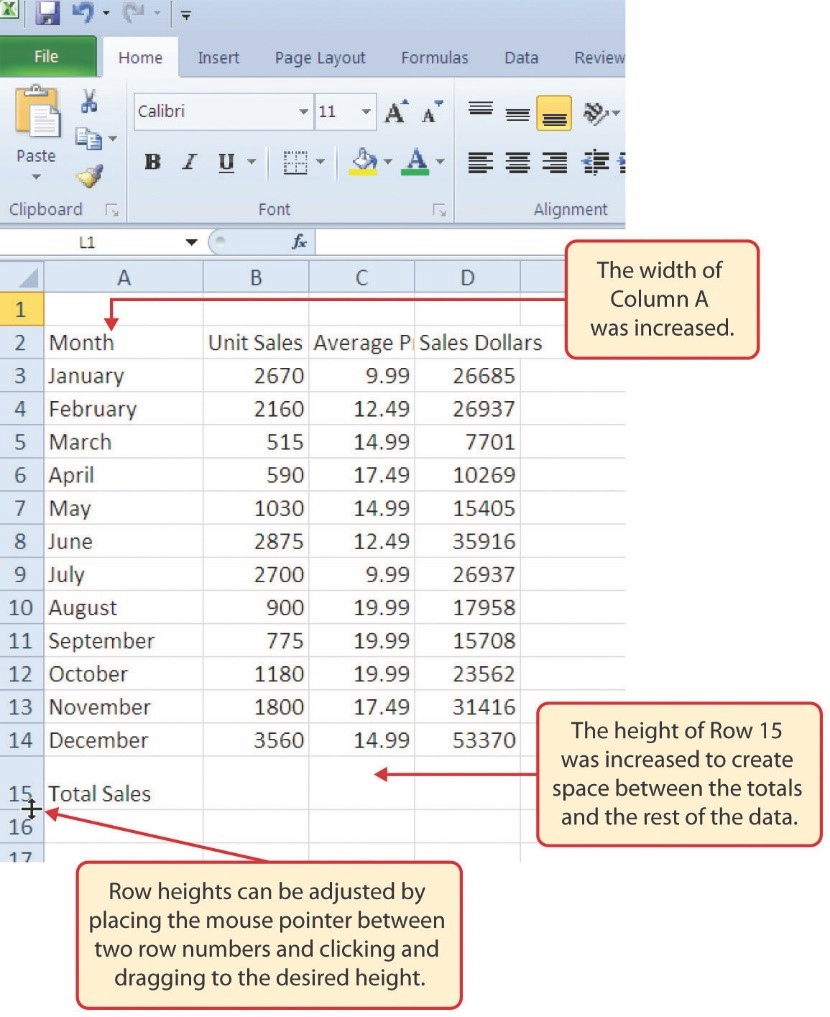
\includegraphics[width=\maxwidth{.95\linewidth}]{gfx/ch01_fig25}
	\caption{CH1-GMW Sales Data with Column A and Row 15 Adjusted}
	\label{01:fig25}
\end{figure}

\begin{center}
	\begin{sklbox}{Skill Refresher}
		\textbf{Adjusting Columns and Rows}
		\\
		\begin{itemize}
			\setlength{\itemsep}{0pt}
			\setlength{\parskip}{0pt}
			\setlength{\parsep}{0pt}
			
			\item Activate at least one cell in the row or column being adjusted.
			\item Click \textit{Home $ \Rightarrow $ Cells $ \Rightarrow $ Format}
			\item Click either \textit{Row Height} or \textit{Column Width} from the drop-down menu.
			\item Enter the Row Height in points or Column Width in characters in the dialog box.
			\item Click the \textit{OK} button.
			
		\end{itemize}
	\end{sklbox}
\end{center}

\subsection{Hiding Columns and Rows}

In addition to adjusting the columns and rows on a worksheet, they can also be hidden. This is a useful technique for enhancing the visual appearance of a worksheet that contains data that is not necessary to display. These features will be demonstrated using the \textit{CH1-GMW Sales Data} workbook later in the course; however, there is no need to have hidden columns or rows in this worksheet. The use of these skills will be presented here for demonstration purposes only.

\begin{enumerate}
	\item Click cell \fmtLoc{C1} in the \fmtWorksheet{Sheet1} worksheet.
	\item Click \fmtButton{Home $ \Rightarrow $ Cells $ \Rightarrow $ Format $ \Rightarrow $ Hide \& Unhide}. This will open a submenu of options.
	\item Click the \fmtButton{Hide Columns} option in the submenu of options (see Figure \ref{01:fig26}) to hide \fmtLoc{Column C}.
\end{enumerate}

\begin{figure}[H]
	\centering
	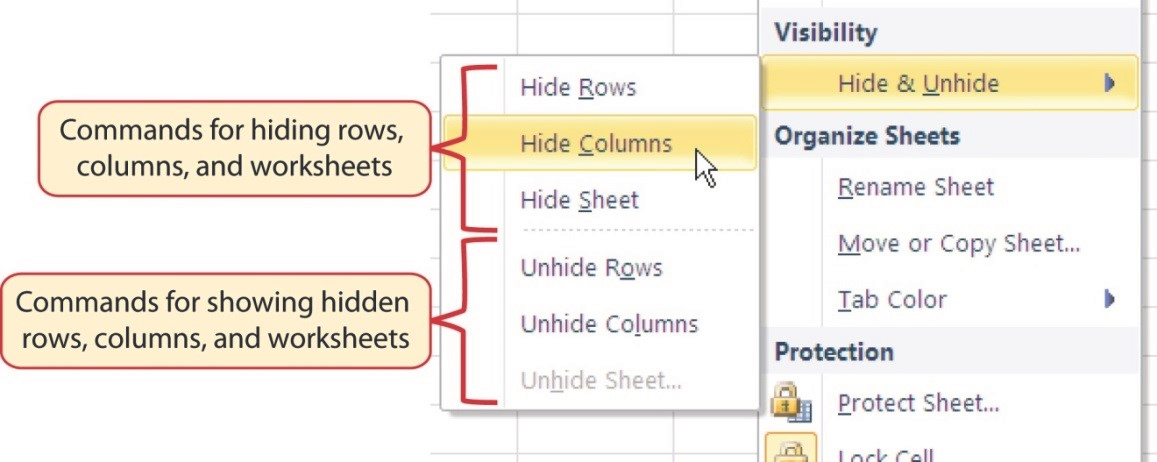
\includegraphics[width=\maxwidth{.95\linewidth}]{gfx/ch01_fig26}
	\caption{Hide \& Unhide Submenu}
	\label{01:fig26}
\end{figure}

\begin{center}
	\begin{shtcutbox}{Keyboard Shortcuts}
		\textbf{Hiding Columns}
		\\
		\begin{itemize}
			\setlength{\itemsep}{0pt}
			\setlength{\parskip}{0pt}
			\setlength{\parsep}{0pt}
			
			\item Hold down the \fmtKeystroke{Ctrl} key while pressing the number \fmtKeystroke{0} on the keyboard. (Note, this is the number zero, not the letter O.)
			
		\end{itemize}
	\end{shtcutbox}
\end{center}

Figure \ref{01:fig27} shows the workbook with \textit{Column C} hidden. If a column is hidden, its name is missing, like the missing letter \textit{C} at the top of the column.

\begin{figure}[H]
	\centering
	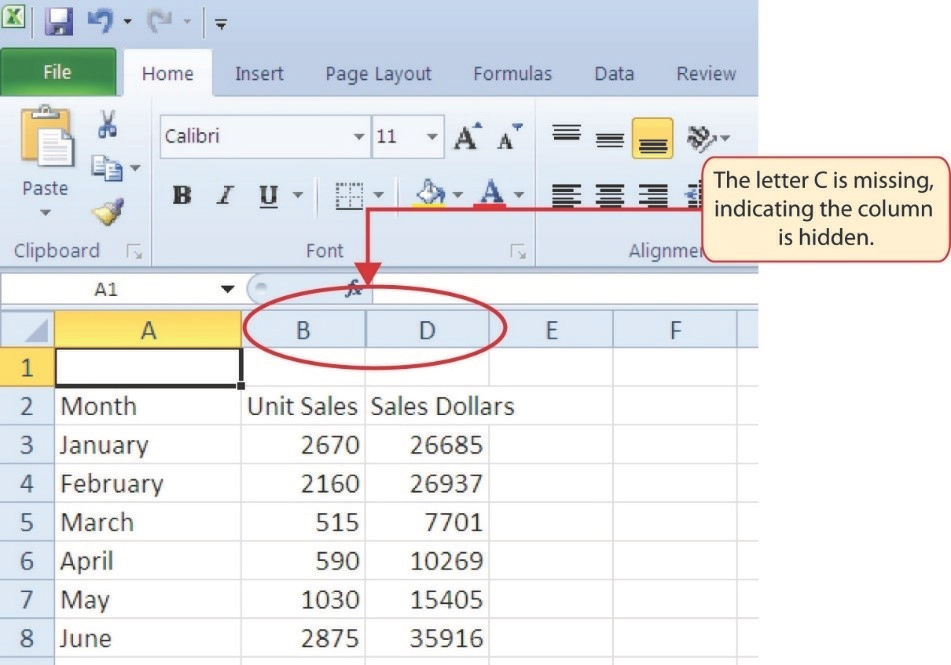
\includegraphics[width=\maxwidth{.95\linewidth}]{gfx/ch01_fig27}
	\caption{Hidden Column}
	\label{01:fig27}
\end{figure}

To unhide a column, use the following steps.

\begin{enumerate}
	\item Highlight the range \fmtLoc{B1:D1} by activating cell \fmtLoc{B1} and clicking and dragging over to cell \fmtLoc{D1}.
	\item Click \fmtButton{Home $ \Rightarrow $ Cells $ \Rightarrow $ Format $ \Rightarrow $ Hide \& Unhide}. 
	\item Click the \fmtButton{Unhide Columns} option in the submenu of options. \fmtLoc{Column C} will now be visible on the worksheet.
\end{enumerate}

\begin{center}
	\begin{shtcutbox}{Keyboard Shortcuts}
		\textbf{Unhiding Columns}
		\\
		\begin{itemize}
			\setlength{\itemsep}{0pt}
			\setlength{\parskip}{0pt}
			\setlength{\parsep}{0pt}
			
			\item Highlight cells on either side of the hidden column(s), then hold down the \fmtKeystroke{Ctrl} key and the \fmtKeystroke{Shift} key while pressing \fmtKeystroke{)}, the close parenthesis key, on the keyboard. Note: This keyboard shortcut does not reliably work for some reason that has not been explained by Microsoft. If it does not work, then use the ribbon button.
			
		\end{itemize}
	\end{shtcutbox}
\end{center}

The following steps demonstrate how to hide rows, which is similar to hiding columns.

\begin{enumerate}
	\item Click cell \fmtLoc{A3} in the \fmtWorksheet{Sheet1} worksheet.
	\item Click \fmtButton{Home $ \Rightarrow $ Cells $ \Rightarrow $ Format $ \Rightarrow $ Hide \& Unhide}. This will open a submenu of options.
	\item Click the \fmtButton{Hide Rows} option in the submenu of options. This will hide \fmtLoc{Row 3}.
\end{enumerate}

\begin{center}
	\begin{shtcutbox}{Keyboard Shortcuts}
		\textbf{Hiding Rows}
		\\
		\begin{itemize}
			\setlength{\itemsep}{0pt}
			\setlength{\parskip}{0pt}
			\setlength{\parsep}{0pt}
			
			\item Hold down the \fmtKeystroke{Ctrl} key while pressing the number \fmtKeystroke{9} key on the keyboard.
			
		\end{itemize}
	\end{shtcutbox}
\end{center}

To unhide a row, follow these steps.

\begin{enumerate}
	\item Highlight the range \fmtLoc{A2:A4} by activating cell \fmtLoc{A2} and clicking and dragging over to cell \fmtLoc{A4}.
	\item Click \fmtButton{Home $ \Rightarrow $ Cells $ \Rightarrow $ Format $ \Rightarrow $ Hide \& Unhide}. This will open a submenu of options.
	\item Click the \fmtButton{Unhide Rows} option in the submenu of options to unhide \fmtLoc{Row 3}.
\end{enumerate}

\begin{center}
	\begin{shtcutbox}{Keyboard Shortcuts}
		\textbf{Unhiding Rows}
		\\
		\begin{itemize}
			\setlength{\itemsep}{0pt}
			\setlength{\parskip}{0pt}
			\setlength{\parsep}{0pt}
			
			\item Highlight cells above and below the hidden row(s), then hold down the \fmtKeystroke{Ctrl} key and the \fmtKeystroke{Shift} key while pressing \fmtKeystroke{(}, the open parenthesis key, on the keyboard.
			
		\end{itemize}
	\end{shtcutbox}
\end{center}

\begin{center}
	\begin{sklbox}{Skill Refresher}
		\textbf{Hiding Columns and Rows}
		\\
		\begin{itemize}
			\setlength{\itemsep}{0pt}
			\setlength{\parskip}{0pt}
			\setlength{\parsep}{0pt}
			
			\item Activate at least one cell in the row(s) or column(s) being hidden.
			\item Click \textit{Home $ \Rightarrow $ Cells $ \Rightarrow $ Format $ \Rightarrow $ Hide \& Unhide}
			\item Click either the \textit{Hide Rows} or \textit{Hide Columns} option.
			
		\end{itemize}
	\end{sklbox}
\end{center}


\begin{center}
	\begin{sklbox}{Skill Refresher}
		\textbf{Unhiding Columns and Rows}
		\\
		\begin{itemize}
			\setlength{\itemsep}{0pt}
			\setlength{\parskip}{0pt}
			\setlength{\parsep}{0pt}
			
			\item Highlight the cells above and below the hidden row(s) or to the left and right of the hidden column(s).
			\item Click \textit{Home $ \Rightarrow $ Cells $ \Rightarrow $ Format $ \Rightarrow $ Hide \& Unhide}
			\item Click either the \textit{Unhide Rows} or \textit{Unhide Columns} option.
			
		\end{itemize}
	\end{sklbox}
\end{center}

\begin{center}
	\begin{infobox}{Integrity Check}
		\textbf{Hidden Rows and Columns}
		\\
		\\
		In most careers, it is common for professionals to use Excel workbooks that have been designed by a coworker. Before using a workbook developed by someone else, always check for hidden rows and columns. It is easy to determine if a row or column is hidden by looking for missing row  numbers or column letters.
	\end{infobox}
\end{center}

\subsection{Inserting Columns and Rows}

Using Excel workbooks that have been created by others is a very efficient way to work because it eliminates the need to create worksheets from scratch. However, to accomplish a specific goal, additional columns or rows may need to be added to a worksheet. In this case, blank columns or rows are inserted into a worksheet as demonstrated below.

\begin{enumerate}
	\item Click cell \fmtLoc{C1} in the \fmtWorksheet{Sheet1} worksheet.
	\item Click \fmtButton{Home $ \Rightarrow $ Cells $ \Rightarrow $ Insert $ \Rightarrow $ Down Arrow} (see Figure \ref{01:fig28}).
\end{enumerate}

\begin{figure}[H]
	\centering
	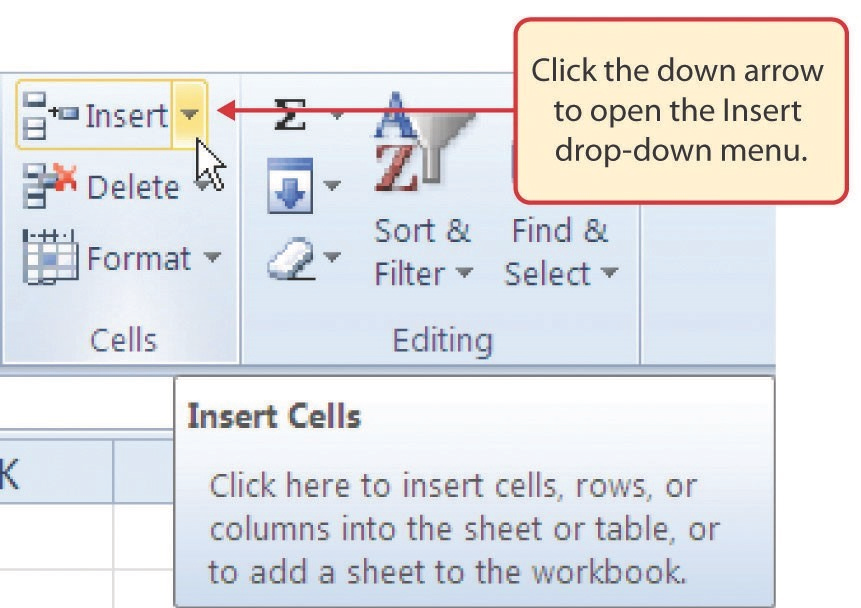
\includegraphics[width=\maxwidth{.95\linewidth}]{gfx/ch01_fig28}
	\caption{Insert Button (Down Arrow)}
	\label{01:fig28}
\end{figure}

\begin{enumerate}[resume]
	\item Click the \fmtButton{Insert Sheet Columns} option from the drop-down menu (see Figure \ref{01:fig29}). A blank column will be inserted to the left of \fmtLoc{Column C}. The contents that were previously in \fmtLoc{Column C} now appear in \fmtLoc{Column D}. Note that columns are always inserted to the left of the activated cell.

\end{enumerate}

\begin{figure}[H]
	\centering
	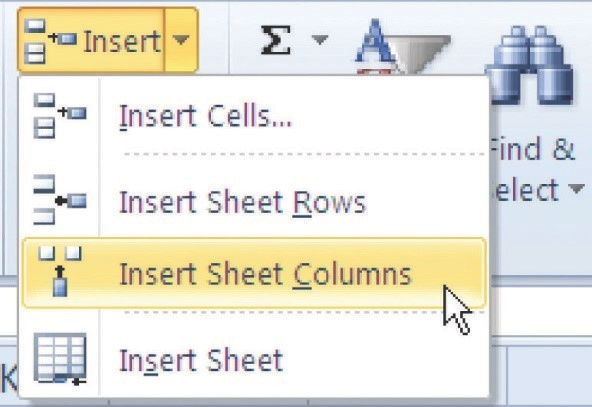
\includegraphics[width=\maxwidth{.95\linewidth}]{gfx/ch01_fig29}
	\caption{Insert Drop-Down Menu}
	\label{01:fig29}
\end{figure}

\begin{center}
	\begin{shtcutbox}{Keyboard Shortcuts}
		\textbf{Inserting Columns}
		\\
		\begin{itemize}
			\setlength{\itemsep}{0pt}
			\setlength{\parskip}{0pt}
			\setlength{\parsep}{0pt}
			
			\item Press the \fmtKeystroke{Alt} key and then the letters \fmtKeystroke{H}, \fmtKeystroke{I}, and \fmtKeystroke{C} one at a time. A column will be inserted to the left of the activated cell.
			
		\end{itemize}
	\end{shtcutbox}
\end{center}

\begin{enumerate}[resume]
	\item Click cell \fmtLoc{A3} in the \fmtWorksheet{Sheet1} worksheet.
	\item Click \fmtButton{Home $ \Rightarrow $ Cells $ \Rightarrow $ Insert $ \Rightarrow $ Down Arrow} (see Figure \ref{01:fig28}).
	\item Click the \fmtButton{Insert Sheet Rows} option from the drop-down menu (see Figure \ref{01:fig29}). A blank row will be inserted above \fmtLoc{Row $ 3 $}. The contents that were previously in \fmtLoc{Row $ 3 $} now appear in \fmtLoc{Row $ 4 $}. Note that rows are always inserted above the activated cell.
\end{enumerate}

\begin{center}
	\begin{shtcutbox}{Keyboard Shortcuts}
		\textbf{Inserting Rpws}
		\\
		\begin{itemize}
			\setlength{\itemsep}{0pt}
			\setlength{\parskip}{0pt}
			\setlength{\parsep}{0pt}
			
			\item Press the \fmtKeystroke{Alt} key and then the letters \fmtKeystroke{H}, \fmtKeystroke{I}, and \fmtKeystroke{R} one at a time. A row will be inserted above the activated cell.
			
		\end{itemize}
	\end{shtcutbox}
\end{center}

\begin{center}
	\begin{sklbox}{Skill Refresher}
		\textbf{Inserting Columns and Rows}
		\\
		\begin{itemize}
			\setlength{\itemsep}{0pt}
			\setlength{\parskip}{0pt}
			\setlength{\parsep}{0pt}
			
			\item Activate the cell to the right of the desired blank column or below the desired blank row.
			\item Click \textit{Home $ \Rightarrow $ Cells $ \Rightarrow $ Insert $ \Rightarrow $ Down Arrow}
			\item Click either the \textit{Insert Sheet Columns} or \textit{Insert Sheet Rows} option.
			
		\end{itemize}
	\end{sklbox}
\end{center}

\subsection{Moving Data}

Once data is entered into a worksheet, it can be moved to different locations, as demonstrated below.

\begin{enumerate}
	\item Highlight the range \fmtLoc{D2:D15} by clicking cell \fmtLoc{D2} and dragging down to cell \fmtLoc{D15}.
	\item Bring the mouse pointer to the left edge of cell \fmtLoc{D2}. Notice that the white block plus sign change to cross arrows (see Figure \ref{01:fig30}). This indicates that the data can be dragged to a new location by left-clicking the mouse.
\end{enumerate}

\begin{figure}[H]
	\centering
	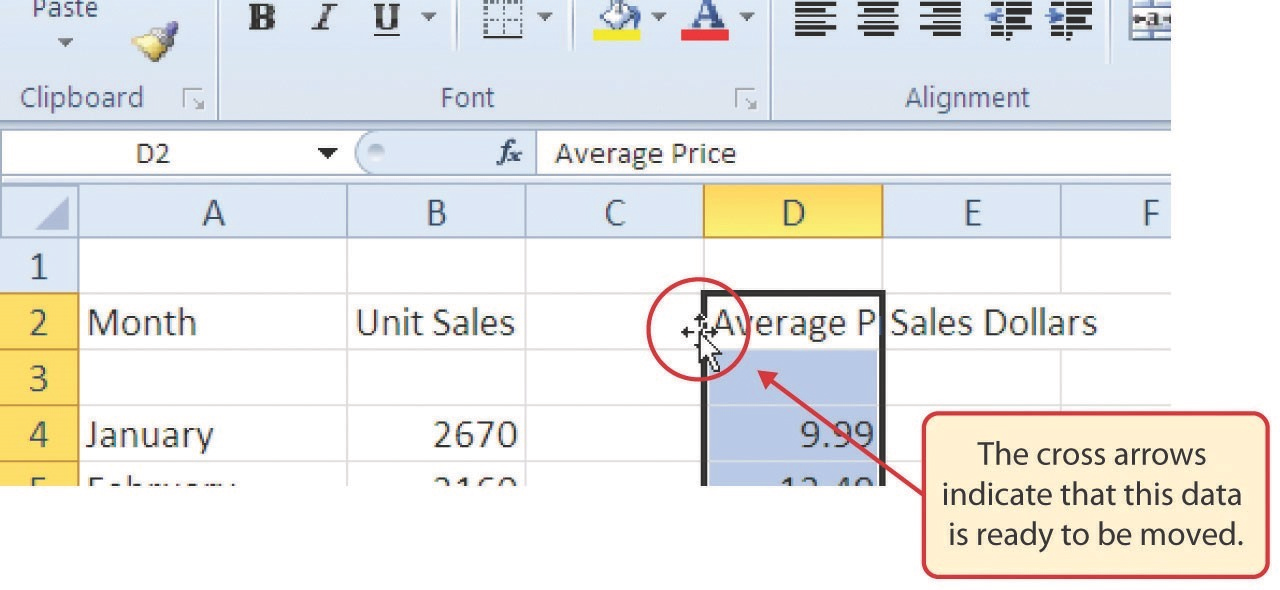
\includegraphics[width=\maxwidth{.95\linewidth}]{gfx/ch01_fig30}
	\caption{Moving Data}
	\label{01:fig30}
\end{figure}

\begin{enumerate}[resume]
	\item Left Click and drag the mouse pointer to cell \fmtLoc{C2}.
	\item Release the left mouse button. The data now appears in \fmtLoc{Column C}.
	\item Click the \textit{Undo} button in the \fmtButton{Quick Access Toolbar}. This moves the data back to \fmtLoc{Column D}.
\end{enumerate}

\begin{center}
	\begin{infobox}{Integrity Check}
		\textbf{Moving Data}
		\\
		\\
		Before moving data on a worksheet, make sure to identify all the components that belong with the series being moved. For example, if a column of data is being moved make sure the column heading is included. Also, make sure all values are highlighted in the column before moving it.
	\end{infobox}
\end{center}


\subsection{Deleting Columns and Rows}

It may occasionally be necessary to delete entire columns or rows of data from a worksheet. For example, a worksheet may contain blank columns or rows that need to be removed. The methods for removing cell contents were covered earlier and can be used to delete unwanted data. However, to delete an entire column or row in a workbook, use the following steps.

\begin{enumerate}
	\item Click cell \fmtLoc{A3}.
	\item Click \fmtButton{Home $ \Rightarrow $ Cells $ \Rightarrow $ Delete $ \Rightarrow $ Down Arrow}
	\item Click the \fmtButton{Delete Sheet Rows} option from the drop-down menu (see Figure \ref{01:fig31}). This removes \fmtLoc{Row 3} and shifts all the data in the worksheet up one row.
\end{enumerate}

\begin{figure}[H]
	\centering
	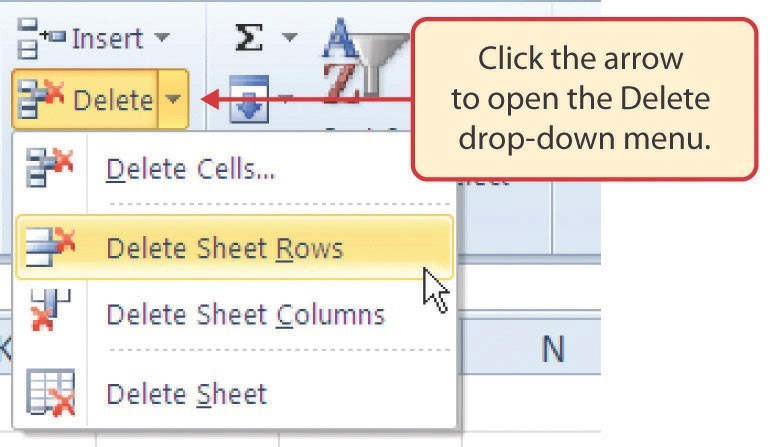
\includegraphics[width=\maxwidth{.95\linewidth}]{gfx/ch01_fig31}
	\caption{Delete Drop-Down Menu}
	\label{01:fig31}
\end{figure}

\begin{center}
	\begin{shtcutbox}{Keyboard Shortcuts}
		\textbf{Deleting Rows}
		\\
		\begin{itemize}
			\setlength{\itemsep}{0pt}
			\setlength{\parskip}{0pt}
			\setlength{\parsep}{0pt}
			
			\item Press the \fmtKeystroke{Alt} key and then the letters \fmtKeystroke{H}, \fmtKeystroke{D}, and \fmtKeystroke{R} one at a time. The row with the activated cell will be deleted.
			
		\end{itemize}
	\end{shtcutbox}
\end{center}

\begin{enumerate}[resume]
	\item Click cell \fmtLoc{C1}.
	\item Click \fmtButton{Home $ \Rightarrow $ Cells $ \Rightarrow $ Delete $ \Rightarrow $ Down Arrow}.
	\item Click the \fmtButton{Delete Sheet Columns} option from the drop-down menu (see Figure \ref{01:fig31}). This removes \fmtLoc{Column C} and shifts all the data in the worksheet over one column to the left.
	\item Save the changes to the workbook by clicking either \fmtButton{Quick Access Toolbar $ \Rightarrow $ Save} or \fmtButton{File $ \Rightarrow $ Save}.
\end{enumerate}

\begin{center}
	\begin{shtcutbox}{Keyboard Shortcuts}
		\textbf{Deleting Columns}
		\\
		\begin{itemize}
			\setlength{\itemsep}{0pt}
			\setlength{\parskip}{0pt}
			\setlength{\parsep}{0pt}
			
			\item Press the \fmtKeystroke{Alt} key and then the letters \fmtKeystroke{H}, \fmtKeystroke{D}, and \fmtKeystroke{C} one at a time. The column with the activated cell will be deleted.
			
		\end{itemize}
	\end{shtcutbox}
\end{center}

\begin{center}
	\begin{sklbox}{Skill Refresher}
		\textbf{Deleting Columns and Rows}
		\\
		\begin{itemize}
			\setlength{\itemsep}{0pt}
			\setlength{\parskip}{0pt}
			\setlength{\parsep}{0pt}
			
			\item Activate any cell in the row or column that is to be deleted.
			\item Click \textit{Home $ \Rightarrow $ Cells $ \Rightarrow $ Delete $ \Rightarrow $ Down Arrow}.
			\item Click either \textit{Delete Sheet Columns} or \textit{Delete Sheet Rows}.
			
		\end{itemize}
	\end{sklbox}
\end{center}

\begin{center}
	\begin{tkwbox}{Key Take-Aways}
		\textbf{Entering, Editing, and Managing Data}
		\\
		\begin{itemize}
			\setlength{\itemsep}{0pt}
			\setlength{\parskip}{0pt}
			\setlength{\parsep}{0pt}
			
			\item Column headings should be used in a worksheet and should accurately describe the data contained in each column.
			\item Using symbols such as dollar signs when entering numbers into a worksheet can slow down the data entry process.
			\item Worksheets must be carefully proofread when data has been manually entered.
			\item The Undo command is a valuable tool for recovering data that was deleted from a worksheet.
			\item When using a worksheet that was developed by someone else, look carefully for hidden columns or rows.
			
		\end{itemize}
	\end{tkwbox}
\end{center}

\section{Formatting and Data Analysis}

\begin{center}
	\begin{objbox}{Learning Objectives}
		\begin{itemize}
			\setlength{\itemsep}{0pt}
			\setlength{\parskip}{0pt}
			\setlength{\parsep}{0pt}
			
			\item Use formatting techniques as introduced in the \textit{Excel Spreadsheet Guidelines}, below, to enhance the appearance of a worksheet.
			\item Understand how to align data in cell locations.
			\item Examine how to enter multiple lines of text in a cell location.
			\item Understand how to add borders to a worksheet.
			\item Examine how to use the AutoSum feature to calculate totals.
			\item Use the Cut, Copy, and Paste commands to manipulate the data on a worksheet.
			\item Understand how to move, rename, insert, and delete worksheet tabs.
		\end{itemize}
	\end{objbox}
\end{center}

This section addresses formatting commands that can be used to enhance the visual appearance of a worksheet. It also provides an introduction to mathematical calculations. The skills introduced in this section provides powerful tools for analyzing the data used in this workbook and will highlight how Excel is used to make key decisions in virtually any career. Additionally, \textit{Excel Spreadsheet Guidelines} for format and appearance will be introduced as a format to be used for the spreadsheets submitted as part of this course.

\subsection{Formatting Data and Cells}

Enhancing the visual appearance of a worksheet is a critical step in creating a valuable tool for coworkers when making key decisions. For example, there are accepted professional formatting standards used when spreadsheets contain only currency data. For this course, the following \textit{Excel Guidelines for Formatting} will be used. Figure \ref{01:fig32} displays how to use Accounting number format when ALL figures are currency. Only the first row of data and the totals should be formatted with the \textit{accounting} format while the other data should be formatted with \textit{comma} style. There also needs to be a top border above the numbers in the total row. If any of the numbers have cents, format all of the data with two decimal places.

\begin{figure}[H]
	\centering
	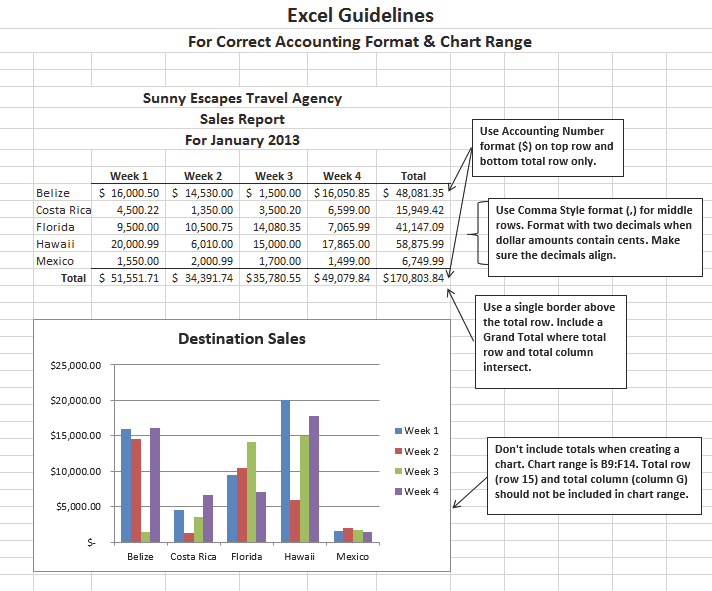
\includegraphics[width=\maxwidth{.95\linewidth}]{gfx/ch01_fig32}
	\caption{Excel Guidelines for Formatting Currency}
	\label{01:fig32}
\end{figure}

Often, Excel spreadsheet contain values that are both currency and non-currency in nature. When that is the case, use the guidelines in Figure \ref{01:fig33}.

\begin{figure}[H]
	\centering
	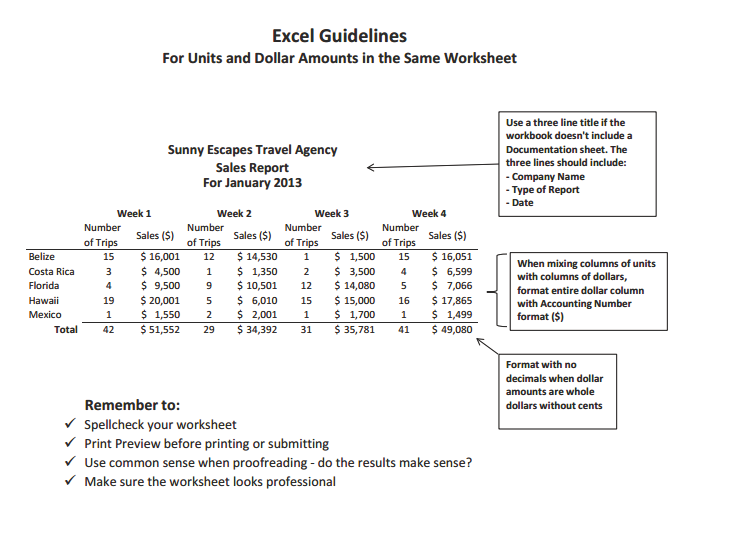
\includegraphics[width=\maxwidth{.95\linewidth}]{gfx/ch01_fig33}
	\caption{Excel Guidelines for Formatting Numbers}
	\label{01:fig33}
\end{figure}

The following steps demonstrate several fundamental formatting skills that will be applied to the workbook developed for this chapter. Several of these formatting skills are identical to ones that may have been used in other Microsoft applications such as Microsoft\textsuperscript{\textregistered} Word\textsuperscript{\textregistered} or Microsoft\textsuperscript{\textregistered} PowerPoint\textsuperscript{\textregistered}.

\begin{enumerate}
	\item Highlight the range \fmtLoc{A2:D2} in the \fmtWorksheet{Sheet1} worksheet by placing the mouse pointer over cell \fmtLoc{A2} and left clicking and dragging to cell \fmtLoc{D2}. 
	\item Click \fmtButton{Home $ \Rightarrow $ Font $ \Rightarrow $ Bold} (see Figure \ref{01:fig34}).
	\item Click \fmtButton{Home $ \Rightarrow $ Font $ \Rightarrow $ Border $ \Rightarrow $ Down Arrow}. Select the \fmtButton{Bottom Border} option from the list to place a border on the bottom of \fmtLoc{Row $ 2 $}.
\end{enumerate}

\begin{figure}[H]
	\centering
	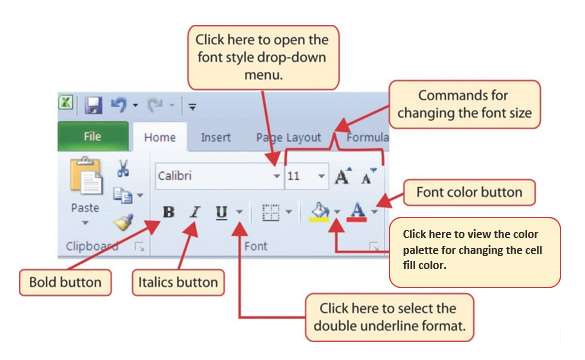
\includegraphics[width=\maxwidth{.95\linewidth}]{gfx/ch01_fig34}
	\caption{Font Group of Commands}
	\label{01:fig34}
\end{figure}

\begin{center}
	\begin{shtcutbox}{Keyboard Shortcuts}
		\textbf{Text Formats}
		\\
		\begin{itemize}
			\setlength{\itemsep}{0pt}
			\setlength{\parskip}{0pt}
			\setlength{\parsep}{0pt}
			
			\item Bold: hold the \fmtKeystroke{Ctrl} key while pressing the letter \fmtKeystroke{B} on the keyboard.
			\item Italics: hold the \fmtKeystroke{Ctrl} key while pressing the letter \fmtKeystroke{I} on the keyboard.
			\item Underline: hold the \fmtKeystroke{Ctrl} key while pressing the letter \fmtKeystroke{U} on the keyboard.
			
		\end{itemize}
	\end{shtcutbox}
\end{center}

\begin{enumerate}[resume]
	\item Highlight the range \fmtLoc{A15:D15} by placing the mouse pointer over cell \fmtLoc{A15} and left clicking and dragging to cell \fmtLoc{D15}.
	\item Click \fmtButton{Home $ \Rightarrow $ Font $ \Rightarrow $ Bold}.
	\item Click \fmtButton{Home $ \Rightarrow $ Font $ \Rightarrow $ Border $ \Rightarrow $ Down Arrow}. Select the \fmtButton{Top Border} option from the list to place a border on the top of \fmtLoc{Row $ 15 $} where totals will eventually be displayed.
	\item Highlight the range \fmtLoc{B3:B14} by placing the mouse pointer over cell \fmtLoc{B3} and left clicking and dragging down to cell \fmtLoc{B14}.
	\item Click \fmtButton{Home $ \Rightarrow $ Number $ \Rightarrow $ Comma Style}. This feature adds a comma and two decimal places to numbers in the cell. (see Figure \ref{01:fig35}).
\end{enumerate}

\begin{figure}[H]
	\centering
	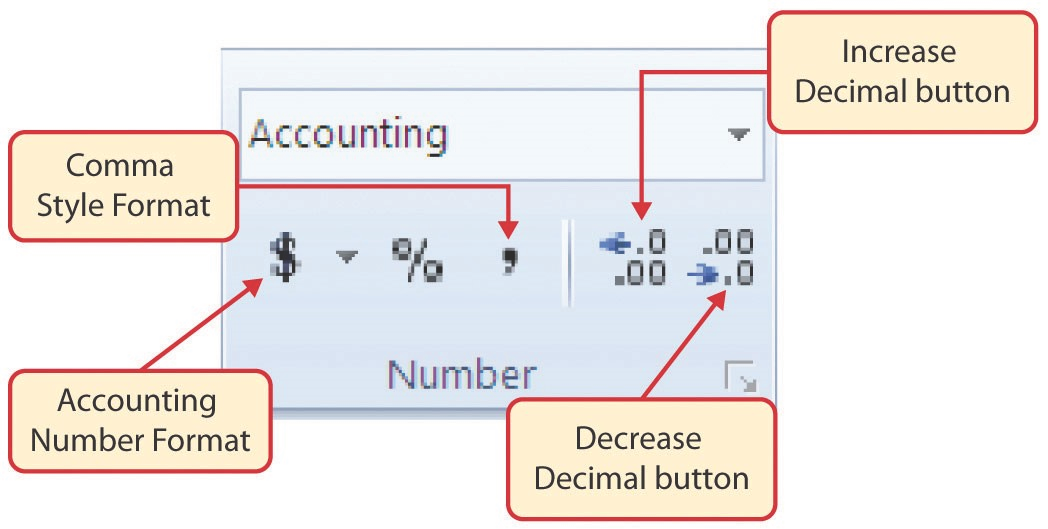
\includegraphics[width=\maxwidth{.95\linewidth}]{gfx/ch01_fig35}
	\caption{Number Group of Commands}
	\label{01:fig35}
\end{figure}

\begin{center}
	\begin{infobox}{Why?}
		\textbf{Format Column Headings and Totals}
		\\
		\\
		Applying formatting enhancements to the column headings and column totals in a worksheet is a very important technique, especially if the workbook will be shared with other people. These formatting techniques allow users of the worksheet to clearly see the column headings that define the data. In addition, the column totals usually contain the most important data on a worksheet with respect to making decisions, and formatting techniques allow users to quickly find this information.
	\end{infobox}
\end{center}


\begin{enumerate}[resume]
	\item Since the figures in this range do not include cents, click \fmtButton{Home $ \Rightarrow $ Number $ \Rightarrow $ Decrease Decimal} two times (see Figure \ref{01:fig35}).
	\item The numbers will be reduced to zero decimal places.
	\item Highlight the range \fmtLoc{C3:C14} by placing the mouse pointer over cell \fmtLoc{C3} and left clicking and dragging down to cell \fmtLoc{C14}.
	\item Click \fmtButton{Home $ \Rightarrow $ Number $ \Rightarrow $ Accounting Number} (see Figure \ref{01:fig35}). This will add a currency symbol and two decimal places to the values, which is common when working with pricing data. As discussed in the Formatting Data and Cells section above, use Accounting format on all values in this range since the worksheet contains non-currency as well as currency data.
	\item Highlight the range \fmtLoc{D3:D14} by placing the mouse pointer over cell \fmtLoc{D3} and left clicking and dragging down to cell \fmtLoc{D14}.
	\item Apply the Accounting Number Format to add the US currency symbol to the values and set them for two decimal places.
	\item Click \fmtButton{Home $ \Rightarrow $ Number $ \Rightarrow $ Decrease Decimal} two times to reduce the decimal places to zero since there are no cents in these figures.
	\item Highlight the range \fmtLoc{A1:D1} by placing the mouse pointer over cell \fmtLoc{A1} and left clicking and dragging over to cell \fmtLoc{D1}.
	\item Click \fmtButton{Home $ \Rightarrow $ Font $ \Rightarrow $ Fill Color $ \Rightarrow $ Down Arrow} (see Figure \ref{01:fig36}). This will prepare the range for a worksheet title.
\end{enumerate}

\begin{figure}[H]
	\centering
	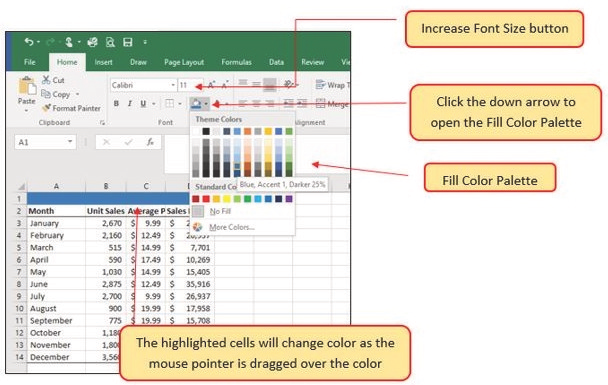
\includegraphics[width=\maxwidth{.95\linewidth}]{gfx/ch01_fig36}
	\caption{Fill Color Palette}
	\label{01:fig36}
\end{figure}

\begin{enumerate}[resume]
	\item Click the \textit{Blue, Accent 1, Darker 25\%} color from the palette (see Figure \ref{01:fig36}). Notice that as the mouse pointer moves over the color palette, a preview of the color appears in the highlighted cells. That makes it easy to experiment with various colors.
	\item Click on \fmtLoc{A1} and enter the worksheet title, \fmtTyping{General Merchandise World}.
	\item Click on \fmtLoc{A2} and then click on \fmtLoc{A1}.This is necessary to select the cell that contains the text rather than the text itself.
	\item Since the black font is difficult to read on the blue background, change the font color to be more visible. Click \fmtButton{Home $ \Rightarrow $ Font $ \Rightarrow $ Font Color $ \Rightarrow $ Down Arrow} and select \textit{White} as the font color for this range (see Figure \ref{01:fig34}).
	\item Highlight the range \fmtLoc{A1:D15} by placing the mouse pointer over cell \fmtLoc{A1} and left clicking and dragging down to cell \fmtLoc{D15}.
	\item Click \fmtButton{Home $ \Rightarrow $ Font $ \Rightarrow $ Down Arrow} and select \textit{Arial} as the font for this range. (see Figure \ref{01:fig34}). Notice that as the mouse pointer moves over the font style options, it changes the highlighted cells. This makes it easy to preview various font options before they are applied.
	\item Expand the column width of \fmtLoc{Column D} to $ 14 $ characters.
\end{enumerate}

Figure \ref{01:fig37} shows how the \fmtWorksheet{Sheet1} worksheet should appear after the formatting techniques are applied.

\begin{figure}[H]
	\centering
	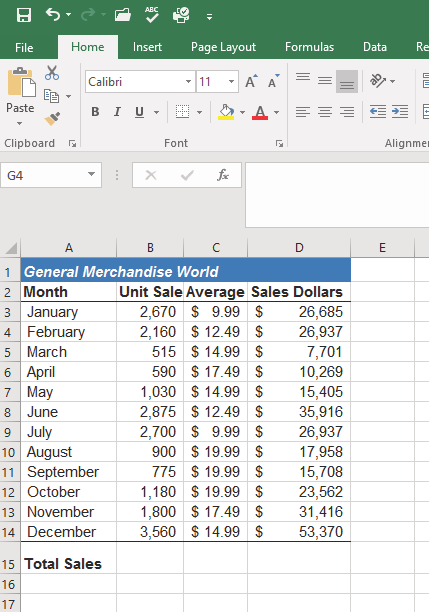
\includegraphics[width=\maxwidth{.95\linewidth}]{gfx/ch01_fig37}
	\caption{Formatting Techniques Applied}
	\label{01:fig37}
\end{figure}

\begin{center}
	\begin{infobox}{Why}
		\textbf{Hashtags (\#\#\#\#) Appear in Columns}
		\\
		\\
		When a column is too narrow for a long number, Excel will automatically convert the number to a series of hashtags (\#\#\#\#). In the case of words or text data, Excel will only show the characters that fit in the column. However, this is not the case with numeric data because it can give the appearance of a number that is much smaller than what is actually in the cell. To remove the hashtags, increase the width of the column.
	\end{infobox}
\end{center}


\subsection{Data Alignment (Wrap Text, Merge Cells, and Center)}

The skills presented in this section show how data is aligned within cell locations. For example, text and numbers can be centered, left aligned, right aligned, and so on within a cell. In some cases multi-word text entries may need to be stacked vertically instead of expanding the width of a column, which is referred to as wrapping text. These skills are demonstrated in the following steps.

\begin{enumerate}
	\item Highlight the range \fmtLoc{B2:D2} by placing the mouse pointer over cell \fmtLoc{B2} and left clicking and dragging over to cell \fmtLoc{D2}.
	\item Click \fmtButton{Home $ \Rightarrow $ Alignment $ \Rightarrow $ Center} (see Figure \ref{01:fig38}). This will center the column headings in each cell location. Notice the difference between text that is centered horizontally and text that is middle aligned vertically.
\end{enumerate}

\begin{figure}[H]
	\centering
	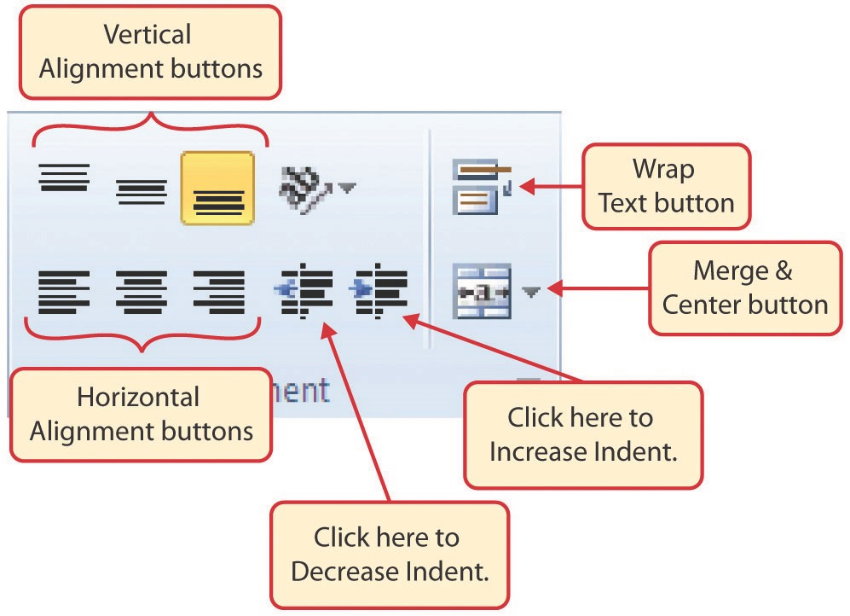
\includegraphics[width=\maxwidth{.95\linewidth}]{gfx/ch01_fig38}
	\caption{Alignment Group in Home Tab}
	\label{01:fig38}
\end{figure}

\begin{enumerate}[resume]
	\item Click \fmtButton{Home $ \Rightarrow $ Alignment $ \Rightarrow $ Wrap Text} (see Figure \ref{01:fig38}). The height of \fmtLoc{Row $ 2 $} automatically expands, and the words that were cut off because the columns were too narrow are now stacked vertically.
\end{enumerate}

\begin{center}
	\begin{shtcutbox}{Keyboard Shortcuts}
		\textbf{Wrap Text}
		\\
		\begin{itemize}
			\setlength{\itemsep}{0pt}
			\setlength{\parskip}{0pt}
			\setlength{\parsep}{0pt}
			
			\item Press the \fmtKeystroke{Alt} key and then the letters \fmtKeystroke{H} and \fmtKeystroke{W} one at a time.
			
		\end{itemize}
	\end{shtcutbox}
\end{center}

\begin{enumerate}[resume]
	\item Highlight the range \fmtLoc{A1:D1} by placing the mouse pointer over cell \fmtLoc{A1} and left clicking and dragging over to cell \fmtLoc{D1}.
	\item Click \fmtButton{Home $ \Rightarrow $ Alignment $ \Rightarrow $ Merge \& Center $ \Rightarrow $ Down Arrow}.
	\item Click the \fmtButton{Merge \& Center} option (see Figure \ref{01:fig39}). This will create one large cell location running across the top of the data set.

\end{enumerate}

\begin{figure}[H]
	\centering
	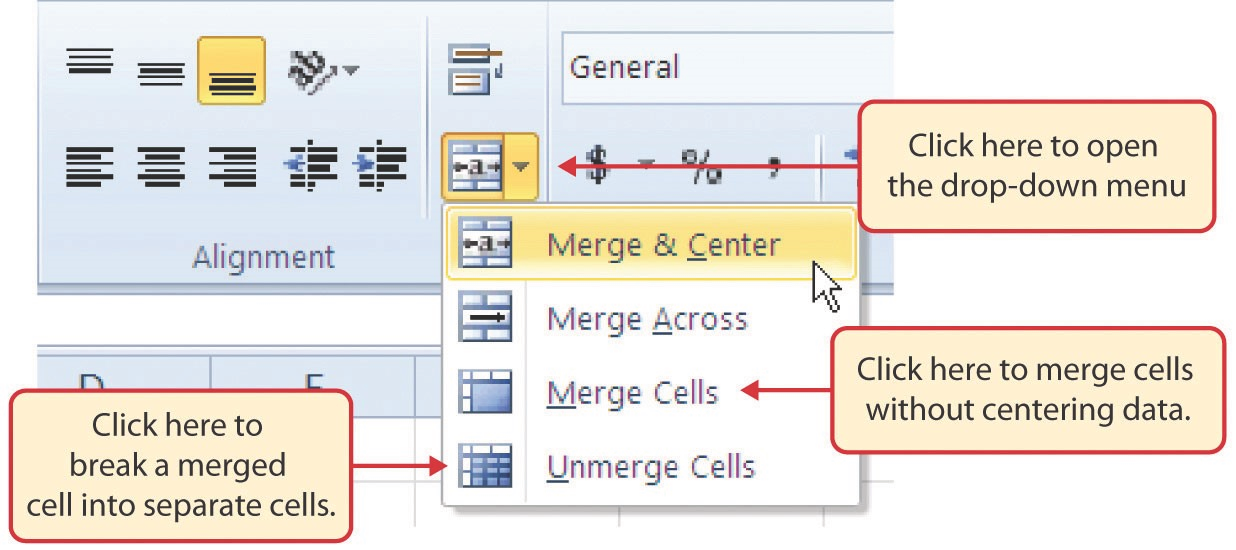
\includegraphics[width=\maxwidth{.95\linewidth}]{gfx/ch01_fig39}
	\caption{Merge Cell Drop-Down Menu}
	\label{01:fig39}
\end{figure}

\begin{center}
	\begin{shtcutbox}{Keyboard Shortcuts}
		\textbf{Merge Commands}
		\\
		\begin{itemize}
			\setlength{\itemsep}{0pt}
			\setlength{\parskip}{0pt}
			\setlength{\parsep}{0pt}
			
			\item \textbf{Merge \& Center}: Press the \fmtKeystroke{Alt} key and then the letters \fmtKeystroke{H}, \fmtKeystroke{M}, and \fmtKeystroke{C} one at a time.
			\item \textbf{Merge Cells}: Press the \fmtKeystroke{Alt} key and then the letters \fmtKeystroke{H}, \fmtKeystroke{M}, and \fmtKeystroke{M} one at a time.
			\item \textbf{Unmerge Cells}: Press the \fmtKeystroke{Alt} key and then the letters \fmtKeystroke{H}, \fmtKeystroke{M}, and \fmtKeystroke{U} one at a time.
			
		\end{itemize}
	\end{shtcutbox}
\end{center}

\begin{center}
	\begin{infobox}{Why?}
		\textbf{Wrap Text}
		\\
		\\
		The benefit of using the Wrap Text command is that it significantly reduces the need to expand the column width to accommodate multi-word column headings. The problem with increasing the column width is that it may reduce the amount of data that can fit on a piece of paper or one screen. This makes it cumbersome to analyze the data in the worksheet and could increase the time it takes to make a decision.
	\end{infobox}
\end{center}

Figure \ref{01:fig40} shows the \textit{Sheet1} worksheet with the data alignment commands applied. The reason for merging the cells in the range $ A1 $:$ D1 $ will become apparent in the next section.

\begin{figure}[H]
	\centering
	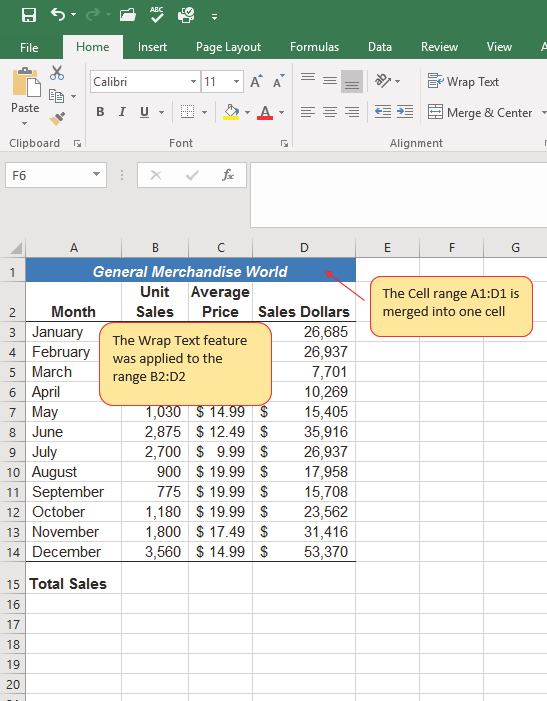
\includegraphics[width=\maxwidth{.95\linewidth}]{gfx/ch01_fig40}
	\caption{Sheet1 with Data Alignment Features Added}
	\label{01:fig40}
\end{figure}

\begin{center}
	\begin{infobox}{Why?}
		\textbf{Merge \& Center}
		\\
		\\
		One of the most common reasons the \fmtButton{Merge \& Center} command is used is to center the title of a worksheet directly above the columns of data. Once the cells above the column headings are merged, a title can be centered above the columns of data. It is very difficult to center the title over the columns of data if the cells are not merged.
	\end{infobox}
\end{center}

\begin{center}
	\begin{sklbox}{Skill Refresher}
		\textbf{Wrap Text}
		\\
		\begin{itemize}
			\setlength{\itemsep}{0pt}
			\setlength{\parskip}{0pt}
			\setlength{\parsep}{0pt}
			
			\item Activate the cell or range of cells that contain text data.
			\item Click \textit{Home $ \Rightarrow $ Alignment $ \Rightarrow $ Wrap Text}.

		\end{itemize}
	\end{sklbox}
\end{center}

\begin{center}
	\begin{sklbox}{Skill Refresher}
		\textbf{Merge Cells}
		\\
		\begin{itemize}
			\setlength{\itemsep}{0pt}
			\setlength{\parskip}{0pt}
			\setlength{\parsep}{0pt}
			
			\item Highlight a range of cells that will be merged.
			\item Click \textit{Home $ \Rightarrow $ Alignment $ \Rightarrow $ Merge \& Center Down Arrow}.
			\item Select an option from the \textit{Merge \& Center} list.
			
		\end{itemize}
	\end{sklbox}
\end{center}

\subsection{Entering Multiple Lines of Text}

In the \textit{Sheet1} worksheet, the cells in the range $ A1 $:$ D1 $ were merged for the purposes of adding a title to the worksheet. This worksheet will contain both a title and a subtitle. The following steps explain how to enter text into a cell and determine where the second line of text should begin.

\begin{enumerate}
	\item Click cell \fmtLoc{A1} in the \fmtWorksheet{Sheet1} worksheet. Since the cells were merged, clicking cell \fmtLoc{A1} will automatically activate the range \fmtLoc{A1:D1}. Position the mouse to the end of the title, directly after the ``d'' in the word ``World'' and double-click to get a cursor (flashing I-beam).
	\item Hold down the \fmtKeystroke{Alt} key and press the \fmtKeystroke{Enter} key. This will start a new line of text in this cell location.
	\item Type the text \fmtTyping{Retail Sales (in millions)} and press the \fmtKeystroke{Enter} key.
	\item Click cell \fmtLoc{A1}. 
	\item Increase the height of Row $ 1 $ to $ 30 $ points. Once the row height is increased, all the text typed into the cell will be visible (see Figure \ref{01:fig41}).
	\item Click \fmtButton{Home $ \Rightarrow $ Font $ \Rightarrow $ Bold}.
	\item Click \fmtButton{Home $ \Rightarrow $ Font $ \Rightarrow $ Italics}.

\end{enumerate}

\begin{figure}[H]
	\centering
	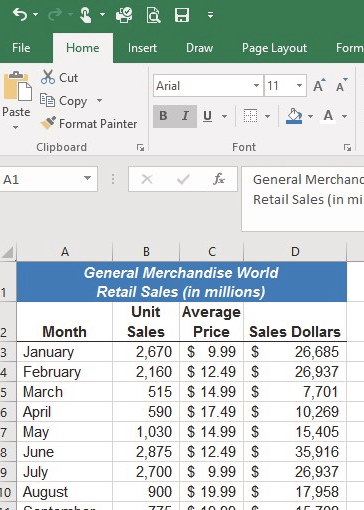
\includegraphics[width=\maxwidth{.95\linewidth}]{gfx/ch01_fig41}
	\caption{Title \& Subtitle Added to the Worksheet}
	\label{01:fig41}
\end{figure}

\begin{center}
	\begin{sklbox}{Skill Refresher}
		\textbf{Entering Multiple Lines of Text}
		\\
		\begin{itemize}
			\setlength{\itemsep}{0pt}
			\setlength{\parskip}{0pt}
			\setlength{\parsep}{0pt}
			
			\item Activate a cell location.
			\item Type the first line of text.
			\item Hold down the \fmtKeystroke{Alt} key and press the \fmtKeystroke{Enter} key.
			\item Type the second line of text and press the \fmtKeystroke{Enter} key.
			
		\end{itemize}
	\end{sklbox}
\end{center}

\subsection{Borders (Adding Lines to a Worksheet)}

In Excel, adding custom lines to a worksheet is known as adding borders. Borders are different from the grid lines that appear on a worksheet and that define the perimeter of the cell locations. Borders add a variety of line styles to a worksheet that can make reading the worksheet much easier. The following steps illustrate methods for adding both preset and custom borders to a worksheet.

\begin{enumerate}
	\item Click \fmtButton{Home $ \Rightarrow $ Font $ \Rightarrow $ Borders $ \Rightarrow $ Down Arrow} to view border options. (see Figure \ref{01:fig42}).
\end{enumerate}

\begin{figure}[H]
	\centering
	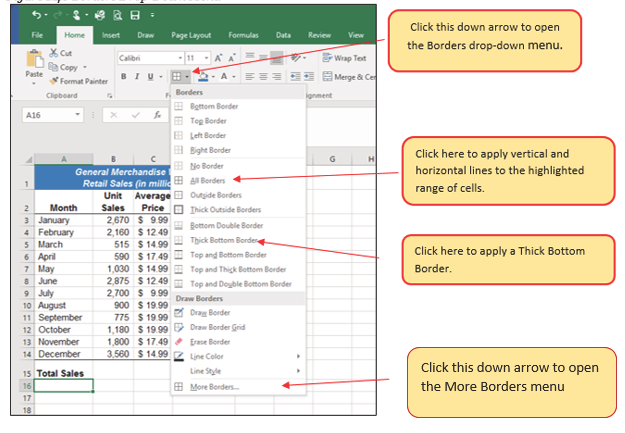
\includegraphics[width=\maxwidth{.95\linewidth}]{gfx/ch01_fig42}
	\caption{Borders Drop-Down Menu}
	\label{01:fig42}
\end{figure}

\begin{enumerate}[resume]
	\item Highlight the range \fmtLoc{A1:D15}. 
	\item Click \fmtButton{Home $ \Rightarrow $ Font $ \Rightarrow $ Borders $ \Rightarrow $ Down Arrow $ \Rightarrow $ All Borders} (see Figure \ref{01:fig42}). This will add vertical and horizontal lines to the range \fmtLoc{A1:D15}.
	\item Highlight the range \fmtLoc{A2:D2} by clicking \fmtLoc{A2} and dragging to cell \fmtLoc{D2}.
	\item Click \fmtButton{Home $ \Rightarrow $ Font $ \Rightarrow $ Borders $ \Rightarrow $ Down Arrow $ \Rightarrow $ Thick Bottom Border}
	\item Highlight the range \fmtLoc{A14:D14} and click \fmtButton{Home $ \Rightarrow $ Font $ \Rightarrow $ Borders $ \Rightarrow $ Down Arrow $ \Rightarrow $ Thick Bottom Border}. The thick border will help maintain the \textit{Excel Formatting Guidelines}.
	\item Highlight the range \fmtLoc{A1:D15}.
	\item Click \fmtButton{Home $ \Rightarrow $ Font $ \Rightarrow $ Borders $ \Rightarrow $ Down Arrow $ \Rightarrow $ More Borders...}
	\item This will open the \textit{Format Cells} dialog box (see Figure \ref{01:fig43}). All Excel formatting commands can be accessed through this dialog box.
	\item In the \textit{Style} section of the \textit{Borders} tab, click the thickest line style (see Figure \ref{01:fig43}).
	\item Click the \fmtButton{Outline} button in the \textit{Presets} section (see Figure \ref{01:fig43}).
	\item Click the \fmtButton{OK} button at the bottom of the dialog box (see Figure \ref{01:fig43}).
\end{enumerate}

\begin{figure}[H]
	\centering
	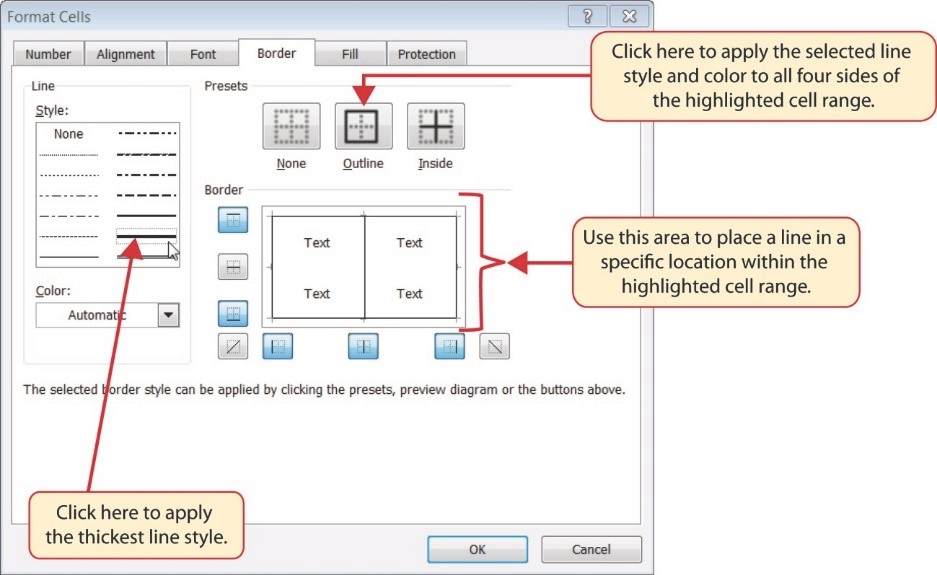
\includegraphics[width=\maxwidth{.95\linewidth}]{gfx/ch01_fig43}
	\caption{Borders Tab of the Format Cells Dialog Box}
	\label{01:fig43}
\end{figure}

The \textit{Sheet1} worksheet should now look like Figure \ref{01:fig44}.

\begin{figure}[H]
	\centering
	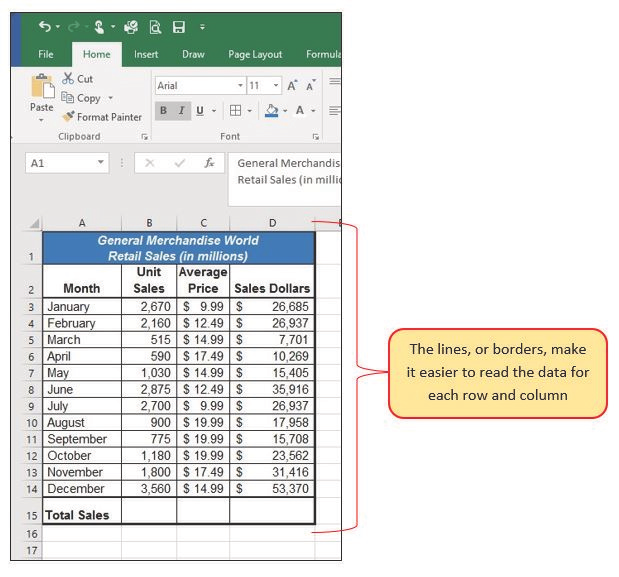
\includegraphics[width=\maxwidth{.95\linewidth}]{gfx/ch01_fig44}
	\caption{Borders Added to the Sheet1 Worksheet}
	\label{01:fig44}
\end{figure}

\begin{center}
	\begin{sklbox}{Skill Refresher}
		\textbf{Preset Borders}
		\\
		\begin{itemize}
			\setlength{\itemsep}{0pt}
			\setlength{\parskip}{0pt}
			\setlength{\parsep}{0pt}
			
			\item Highlight a range of cells that require borders.
			\item Click the \textit{Home} tab of the Ribbon.
			\item Click the down arrow next to the \textit{Borders} button.
			\item Select an option from the preset borders list.
			
		\end{itemize}

		\hfill \break
		\textbf{Custom Borders}
		\\
		\begin{itemize}
			\setlength{\itemsep}{0pt}
			\setlength{\parskip}{0pt}
			\setlength{\parsep}{0pt}
			
			\item Highlight a range of cells that require borders.
			\item Click \textit{Home $ \Rightarrow $ Font $ \Rightarrow $ Borders $ \Rightarrow $ Down Arrow $ \Rightarrow $ More Borders...}
			\item Select a line style and line color.
			\item Select a placement option.
			\item Click the \textit{OK} button on the dialog box.
			
		\end{itemize}

	\end{sklbox}
\end{center}

\subsection{Autosum}

Notice at the bottom of Figure \ref{01:fig44} that \textit{Row 15} is intended to show the totals for the data in this worksheet. Applying mathematical computations to a range of cells is accomplished through functions in Excel\footnote{Chapter \ref{ch03:formulas}, \nameref{ch03:formulas}, page \pageref{ch03:formulas}, in this book reviews mathematical formulas and functions in detail.}. The following steps will demonstrate how to quickly sum the values in a column of data using the AutoSum command.

\begin{enumerate}
	\item Click in cell \fmtLoc{B15} in the \fmtWorksheet{Sheet1} worksheet.
	\item Click \fmtButton{Formulas $ \Rightarrow $ Function Library $ \Rightarrow $ AutoSum $ \Rightarrow $ Down Arrow} (see Figure \ref{01:fig45}). Note that autosum can also be found at \fmtButton{Home $ \Rightarrow $ Editing $ \Rightarrow $ AutoSum}.
\end{enumerate}

\begin{figure}[H]
	\centering
	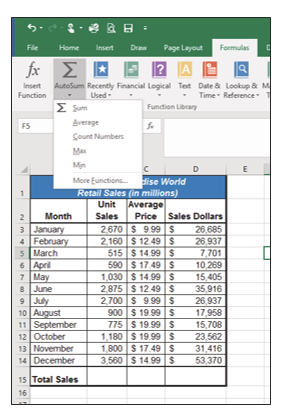
\includegraphics[width=\maxwidth{.95\linewidth}]{gfx/ch01_fig45}
	\caption{AutoSum Drop-Down List}
	\label{01:fig45}
\end{figure}

\begin{enumerate}[resume]
	\item Click the \fmtButton{Sum} option from the \textit{AutoSum} drop-down menu. The first click will display a flashing marquee around the range. Press the \fmtKeystroke{Enter} key or click the \fmtButton{Check Mark} next to the Formula bar to complete the function.
	\item Excel will provide a total for the values in the \textit{Unit Sales} column.
	\item It would not make sense to total the averages in \fmtLoc{Column C} so \fmtLoc{C15} will be left blank.
	\item Click in cell \fmtLoc{D15}. 
	\item Click \fmtButton{Formulas $ \Rightarrow $ Function Library $ \Rightarrow $ AutoSum $ \Rightarrow $ Down Arrow}. 
	\item Click the \fmtButton{Sum} option from the \textit{AutoSum} drop-down menu. The first click will display a flashing marquee around the range. Press the \fmtKeystroke{Enter} key or click the \fmtButton{Check Mark} next to the Formula bar to complete the function. (see Figure \ref{01:fig46}).
\end{enumerate}

\begin{figure}[H]
	\centering
	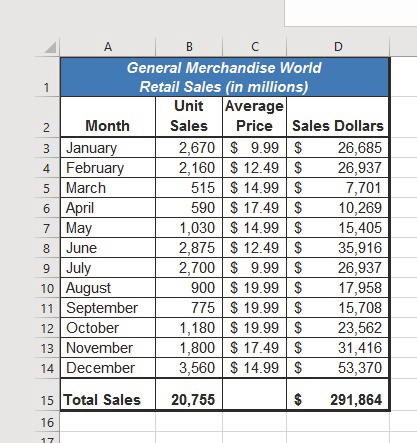
\includegraphics[width=\maxwidth{.95\linewidth}]{gfx/ch01_fig46}
	\caption{Totals Added to the Sheet1 Worksheet}
	\label{01:fig46}
\end{figure}

\begin{center}
	\begin{sklbox}{Skill Refresher}
		\textbf{AutoSum}
		\\
		\begin{itemize}
			\setlength{\itemsep}{0pt}
			\setlength{\parskip}{0pt}
			\setlength{\parsep}{0pt}
			
			\item Highlight a cell location below or to the right of a range of cells that contain numeric values.
			\item Click the \textit{Formulas} tab of the Ribbon.
			\item Click the down arrow below the \textit{AutoSum} button.
			\item Select a mathematical function from the list.
			
		\end{itemize}
	\end{sklbox}
\end{center}

\subsection{Moving, Renaming, Inserting, and Deleting Worksheets}

The default names for the worksheet tabs at the bottom of workbook are \textit{Sheet1}, \textit{Sheet2}, and so on. However, the worksheet names can be changed to identify the data each worksheet contains. Additionally, the order that the worksheet tabs appear can be changed. The following steps explain how to rename and move the worksheets in a workbook.

\begin{enumerate}
	\item Double-click the \fmtWorksheet{Sheet1} worksheet tab at the bottom of the workbook (see Figure \ref{01:fig47}). 
	\item Type the name \fmtTyping{Sales by Month} and press \fmtKeystroke{Enter}.
	\item Double click the \fmtWorksheet{Sheet2} worksheet tab at the bottom of the workbook.
	\item Type the name \fmtTyping{Unit Sales Rank} and press \fmtKeystroke{Enter}.
\end{enumerate}

\begin{figure}[H]
	\centering
	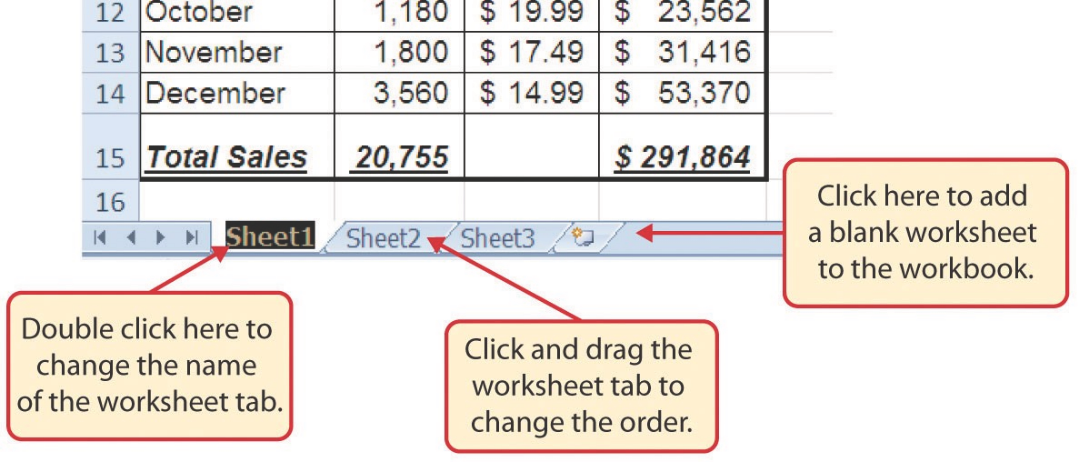
\includegraphics[width=\maxwidth{.95\linewidth}]{gfx/ch01_fig47}
	\caption{Renaming a Worksheet Tab}
	\label{01:fig47}
\end{figure}

\begin{enumerate}
	\item Click-and-drag the \fmtWorksheet{Unit Sales Rank} worksheet tab to the left of the \fmtWorksheet{Sales by Month} sheet. It will become the first worksheet in the workbook.
	\item Click the \fmtWorksheet{Sheet3} worksheet tab.
	\item Click \fmtButton{Home $ \Rightarrow $ Cells $ \Rightarrow $ Delete $ \Rightarrow $ Down Arrow $ \Rightarrow $ Delete Sheet}. This removes the unneeded worksheet.
	\item If a warning box pops up, click the \fmtButton{Delete} button.
	\item Also delete the \fmtWorksheet{Unit Sales Rank} worksheet since it was decided that worksheet is also unnecessary. This means that the workbook is left with just one worksheet, \fmtWorksheet{Sales by Month}.
	\item Save the changes to the workbook by clicking either \fmtButton{Quick Access Toolbar $ \Rightarrow $ Save} or \fmtButton{File $ \Rightarrow $ Save}.
\end{enumerate}

\begin{center}
	\begin{infobox}{Integrity Check}
		\textbf{Deleting Worksheets}
		\\
		\\
		Be very cautious when deleting worksheets that contain data. Once a worksheet is deleted it is gone forever; the Undo command cannot bring the sheet back. \textit{Deleting a worksheet is permanent!}
	\end{infobox}
\end{center}

\begin{center}
	\begin{shtcutbox}{Keyboard Shortcuts}
		\textbf{Inserting New Worksheets}
		\\
		\begin{itemize}
			\setlength{\itemsep}{0pt}
			\setlength{\parskip}{0pt}
			\setlength{\parsep}{0pt}
			
			\item Press the \fmtKeystroke{Shift} key and then the \fmtKeystroke{F11} key on the keyboard.
			
		\end{itemize}
	\end{shtcutbox}
\end{center}


Figure \ref{01:fig48} shows the final appearance of the \textit{CH1-GMW Sales} workbook.

\begin{figure}[H]
	\centering
	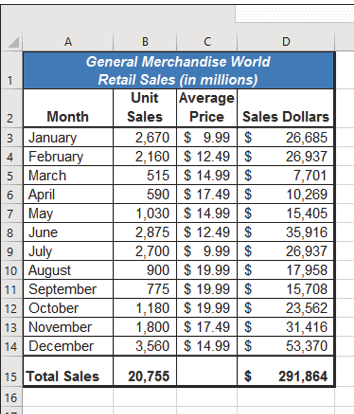
\includegraphics[width=\maxwidth{.95\linewidth}]{gfx/ch01_fig48}
	\caption{Final Appearance of the CH1-GMW Sales Workbook}
	\label{01:fig48}
\end{figure}

\begin{center}
	\begin{sklbox}{Skill Refresher}
		\textbf{Renaming Worksheets}
		\\
		\begin{itemize}
			\setlength{\itemsep}{0pt}
			\setlength{\parskip}{0pt}
			\setlength{\parsep}{0pt}
			
			\item Double click the worksheet tab.
			\item Type the new name.
			\item Press the \fmtKeystroke{Enter} key.
		\end{itemize}

		\hfill \break
		\textbf{Moving Worksheets}
		\\
		\begin{itemize}
			\setlength{\itemsep}{0pt}
			\setlength{\parskip}{0pt}
			\setlength{\parsep}{0pt}
			
			\item Left click the worksheet tab.
			\item Drag it to the desired position.
		\end{itemize}

		\hfill \break
		\textbf{Deleting Worksheets}
		\\
		\begin{itemize}
			\setlength{\itemsep}{0pt}
			\setlength{\parskip}{0pt}
			\setlength{\parsep}{0pt}
			
			\item Open the worksheet to be deleted.
			\item Click \textit{Home $ \Rightarrow $ Cells $ \Rightarrow $ Delete $ \Rightarrow $ Down Arrow $ \Rightarrow $ Delete Sheet}.
			\item Click \textit{Delete} on the warning box.
		\end{itemize}

	\end{sklbox}
\end{center}

\begin{center}
	\begin{infobox}{Best Practice}
		\textbf{Summary Worksheet}
		\\
		\\
		It is considered a best practice to make the first worksheet in a workbook a summary. That sheet should include the purpose of the workbook and a brief explanation for each of the sheets in the book. It should also include contact information for the originator so questions that may come up later can be clarified. The simple workbooks in this course will not include a summary sheet, but it would be included in more complex projects.
	\end{infobox}
\end{center}


\begin{center}
	\begin{tkwbox}{Key Take-Aways}
		\textbf{Save}
		\\
		\begin{itemize}
			\setlength{\itemsep}{0pt}
			\setlength{\parskip}{0pt}
			\setlength{\parsep}{0pt}
			
			\item Formatting skills are critical for creating worksheets that are easy to read and have a professional appearance.
			\item A series of hashtags (\#\#\#\#) in a cell location indicates that the column is too narrow to display the number entered.
			\item Using the Wrap Text command allows multi-word column headings to be stacked vertically in a cell location, reducing the need to expand column widths.
			\item Use the \textit{Merge \& Center} command to center the title of a worksheet directly over the columns that contain data.
			\item Adding borders or lines will make the worksheet easier to read and helps to separate the data in each column and row.
			\item The Undo command will not bring back a worksheet that has been deleted.
		
		\end{itemize}
	\end{tkwbox}
\end{center}

\section{Printing}

\begin{center}
	\begin{objbox}{Learning Objectives}
		\begin{itemize}
			\setlength{\itemsep}{0pt}
			\setlength{\parskip}{0pt}
			\setlength{\parsep}{0pt}
			
			\item Use the \textit{Page Layout} tab to prepare a worksheet for printing.
			\item Add headers and footers to a printed worksheet.
			\item Explore how to print worksheets and workbooks.
		\end{itemize}
	\end{objbox}
\end{center}

Once a workbook is completed, it is good practice to select the appropriate settings for printing. These settings are in the \textit{Page Layout} tab of the Ribbon and discussed in this section of the chapter.

\subsection{Page Setup}

Before the worksheets in a workbook can be properly printed, the setting must be adjusted. The following steps explain several of the commands in the \textit{Page Layout} tab of the Ribbon used to prepare a worksheet for printing.

\begin{enumerate}
	\item Open the \fmtWorksheet{CH1-GMW Sales} workbook if it is not already open.
	\item Click \fmtButton{Page Layout $ \Rightarrow $ Page Setup $ \Rightarrow $ Margins}. This will open a drop-down list of options for setting the margins of the printed document. The \fmtButton{Normal}, \fmtButton{Wide}, and \fmtButton{Narrow} will quickly apply one of those common margin settings and for this worksheet, click \fmtButton{Narrow}.
	\item To further adjust the margin settings, \fmtButton{Page Layout $ \Rightarrow $ Page Setup $ \Rightarrow $ Margins $ \Rightarrow $ Custom Margins}.
	\item On the \textit{Page Setup} dialog box, click the \fmtButton{Page} tab, then select \fmtButton{Landscape}.
	\item Click the \textit{Margins} tab and locate the \fmtButton{Center on Page} section. Click the boxes to Horizontally and Vertically center the data on the worksheet. (see Figure \ref{01:fig49})
	\item Click \fmtButton{OK}.
\end{enumerate}

\begin{figure}[H]
	\centering
	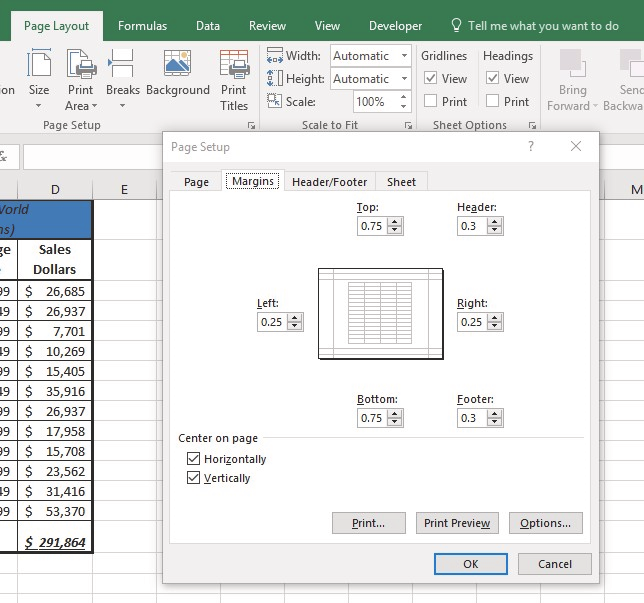
\includegraphics[width=\maxwidth{.95\linewidth}]{gfx/ch01_fig49}
	\caption{Page Layout Commands for Printing}
	\label{01:fig49}
\end{figure}

\begin{center}
	\begin{infobox}{Why?}
		\textbf{Use Print Settings}
		\\
		\\
		Because professionals often share Excel workbooks, it is a good practice to select the appropriate print settings in the \textit{Page Layout} tab even if there is no intent to print the worksheets. It can be extremely frustrating for recipients of a workbook who wish to print the worksheets to find that the necessary print settings have not been selected. 
	\end{infobox}
\end{center}

Table \ref{01:tab02} lists the various page layout settings and how they would be used.

\begin{table}[H]
	\rowcolors{1}{}{tablerow} % zebra striping background
	{\fontsize{8}{10} \selectfont %\small
		%\fontsize{8}{10} \selectfont %Replace small for special font size
		\begin{longtable}{L{0.75in}L{1.75in}L{1.75in}} %Left-aligned, Max width: 4.25in
			\textbf{Command} & \textbf{Purpose} & \textbf{Use} \endhead
			\hline
			Margins & Sets the top, bottom, right, and left margin space for the printed document & 1. Click the Page Layout tab of the Ribbon.\newline2. Click the Margin button.\newline3. Click one of the preset margin options or click Custom Margins.\\
			Orientation & Sets the orientation of the printed document to either portrait or landscape & 1. Click the Page Layout tab of the Ribbon.\newline2. Click the Orientation button.\newline3. Click one of the preset orientation options.\\
			Size & Sets the paper size for the printed document & 1. Click the Page Layout tab of the Ribbon.\newline2. Click the Size button.\newline3. Click one of the preset paper size options or click More Paper Sizes. \\
			Print Area & Used for printing only a specific area or range of cells on a worksheet & 1. Highlight the range of cells on a worksheet to be printed.\newline2. Click the Page Layout tab of the Ribbon.\newline3. Click the Print Area button.\newline4. Click the Set Print Area option from the drop-down list. \\
			Breaks & Manually set the page breaks on a worksheet & 1. Activate a cell on the worksheet where the page break should be placed. Breaks are created above and to the left of the activated cell.\newline2. Click the Page Layout tab of the Ribbon.\newline3. Click the Breaks button.\newline4. Click the Insert Page Break option from the drop-down list. \\
			Background & Adds a picture behind the cell locations in a worksheet & 1. Click the Page Layout tab of the Ribbon.\newline2. Click the Background button.\newline3. Select a picture stored on the local computer or network. \\
			Print Titles & Used when printing large data sets that are several pages long. This command will repeat the column headings at the top of each printed page. & 1. Click the Page Layout tab of the Ribbon.\newline2. Click the Print Titles button.\newline3. Click in the Rows to Repeat at Top input box in the Page Setup dialog box.\newline4. Click any cell in the row that contains the column headings for the worksheet.\newline5. Click the OK button at the bottom of the Page Setup dialog box. \\

			\rowcolor{captionwhite}
			\caption{Purpose and Use for Page Setup Commands}
			\label{01:tab02}
		\end{longtable}
	} % End small
\end{table}

\subsection{Headers and Footers}

When printing worksheets from Excel, it is common to add headers and footers to the printed document. Information in the header or footer could include the date, page number, file name, company name, and so on. The following steps explain how to add headers and footers to the \textit{CH1-GMW Sales Data} workbook.

\begin{enumerate}
	\item Click \fmtButton{Insert $ \Rightarrow $ Text $ \Rightarrow $ Header \& Footer}. 
\end{enumerate}

Note: A new tab containing header and footer controls is added to the ribbon. \fmtOldExcel{Excel 2016} names the tab \textit{Design} and \fmtNewExcel{Excel 365} names it \textit{Header \& Footer}. Other than the name of the tab, the next few instructions are the same for both versions of Excel. Inserting a header or footer will also open the \textit{Page Layout} view of the worksheet, which makes it easy to add elements like the date or page number. Figure \ref{01:fig50} shows the tab that is used to work with headers and footers.

\begin{figure}[H]
	\centering
	\includegraphics[width=\maxwidth{.95\linewidth}]{gfx/ch01_fig50}
	\caption{Tab for Creating Headers and Footers}
	\label{01:fig50}
\end{figure}

\begin{enumerate}[resume]
	\item Type the author's name in the center section of the Header.
	\item Click in the left section of the Header (see Figure \ref{01:fig50}).
	\item Click \fmtButton{Design $ \Rightarrow $ Header \& Footer Elements $ \Rightarrow $ Current Date}. Note: the date will display as \textit{\&[Date]} until the workbook is printed or the normal view is restored.
	\item Click \fmtButton{Design $ \Rightarrow $ Navigation $ \Rightarrow $ Go To Footer}.
	\item Click in the right section of the footer.
	\item Click \fmtButton{Design $ \Rightarrow $ Header \& Footer $ \Rightarrow $ Page Number}. Note: the page number will display as \textit{\&[Page]} until the workbook is printed or the normal view is restored.
	\item Click any cell location outside the header or footer area.
	\item Click the \fmtButton{Normal} view button in the lower right side of the Status Bar (see Figure \ref{01:fig51}).

\end{enumerate}

\begin{figure}[H]
	\centering
	\includegraphics[width=\maxwidth{.95\linewidth}]{gfx/ch01_fig51}
	\caption{Worksheet in Page Layout View}
	\label{01:fig51}
\end{figure}

\subsection{Printing Worksheets and Workbooks}

Once the print settings have been adjusted and the headers and footers added, it is time to print the worksheet. The following steps explain how to print the worksheet in the \textit{CH1-GMW Sales} workbook.

\begin{enumerate}
	\item Click the \fmtButton{File} tab on the Ribbon.
	\item Click the \fmtButton{Print} option on the left side of the \textit{Backstage} view (see Figure \ref{01:fig52}). Notice that there is a preview of the printed worksheet on the right side of the \textit{Backstage} view.
\end{enumerate}

\begin{figure}[H]
	\centering
	\includegraphics[width=\maxwidth{.95\linewidth}]{gfx/ch01_fig52}
	\caption{Backstage View Print option}
	\label{01:fig52}
\end{figure}

\begin{enumerate}[resume]
	\item Click the \fmtButton{Print Active Sheets} button in the \fmtButton{Print} section of the \textit{Backstage} view (see Figure \ref{01:fig52}).
	\item Click the \fmtButton{Print} button to print the active sheet.
	\item Click the \fmtButton{Home} tab of the Ribbon.
	\item Save and close the \fmtWorksheet{CH1-GMW Sales Data} workbook.
	\item Compare the worksheet with the self-check answer key (\fmtWorksheet{CH1-GMW Sales Data Soln}) and then submit the \fmtWorksheet{CH1-GMW Sales} workbook as directed by the instructor.
\end{enumerate}

\begin{center}
	\begin{tkwbox}{Key Take-Aways}
		\textbf{Print}
		\\
		\begin{itemize}
			\setlength{\itemsep}{0pt}
			\setlength{\parskip}{0pt}
			\setlength{\parsep}{0pt}

			\item The commands in the Page Layout tab of the Ribbon are used to prepare a worksheet for printing.
			\item Headers and footers can be added to a worksheet to show key information such as page numbers, the date, the file name, author's name, and so on.
			\item The \fmtButton{Print} commands are in the \fmtButton{File} tab of the Ribbon.
			
		\end{itemize}
	\end{tkwbox}
\end{center}

\section{Chapter Practice}

\subsection{Basic Monthly Budget for a Medical Office}

Creating and maintaining budgets are common practices in many careers. Budgets play a critical role in helping a business or household control expenditures. In this exercise a budget for a hypothetical medical office will be created while reviewing the skills covered in this chapter.

\begin{enumerate}
	\item Open the file named \fmtWorksheet{PR1-Data}, then save as \fmtWorksheet{PR1-Medical Office Budget}.
	\item Activate all the cell locations in the \fmtWorksheet{Sheet1} worksheet by clicking the \fmtButton{Select All} button in the upper left corner of the worksheet (See Figure \ref{01:fig53}).
\end{enumerate}

\begin{figure}[H]
	\centering
	\includegraphics[width=\maxwidth{.95\linewidth}]{gfx/ch01_fig53}
	\caption{The Select All Button}
	\label{01:fig53}
\end{figure}

\begin{enumerate}[resume]
	\item In the \fmtButton{Home} tab of the Ribbon, set the font style to Arial and the font size to $ 12 $ points. Then click any cell to deselect the worksheet.
	\item Double-click the divider between the tops of \fmtLoc{Column A} and \fmtLoc{Column B} to automatically change the width of \fmtLoc{Column A} so all the entries in the range \fmtLoc{A3:A8} are visible. 
	\item Click in \fmtLoc{B2} and enter \fmtTyping{Quarter 1}.
	\item Use the \fmtButton{Auto Fill Handle} to complete the headings in the range \fmtLoc{C2:E2}. Click in cell \fmtLoc{B2} and place the mouse pointer over the \fmtButton{Auto Fill Handle}. When the mouse pointer changes to a black plus sign, left click and drag it to cell \fmtLoc{E2}.
	\item Click \fmtLoc{B2:E2} to select those cells. 
	\item Click \fmtButton{Home $ \Rightarrow $ Cells $ \Rightarrow $ Format $ \Rightarrow $ Column Width}. Set the column width to $ 11.57 $.
	\item Click \fmtLoc{A1} and enter \fmtTyping{Medical Office Budget}.
	\item Click on \fmtLoc{B1} and then click \fmtButton{Home $ \Rightarrow $ Cells $ \Rightarrow $ Insert $ \Rightarrow $ Insert Sheet Columns}.
	\item Click \fmtLoc{B2} and enter \fmtTyping{Budget Cost}.
	\item Adjust the width of \fmtLoc{Column B} to approximately $ 13.25 $ characters.
	\item Click-and-drag from \fmtLoc{A1} to \fmtLoc{F1} to select that range. 
	\item Click \fmtButton{Home $ \Rightarrow $ Alignment $ \Rightarrow $ Merge \& Center}.
	\item Make the following format adjustments to the merged range \fmtLoc{A1:F1}: bold; italics; change the font size to $ 14 $ points; change the cell fill color to Aqua-Accent $ 5 $-Darker $ 50 $\%, and change the font color to \textit{white}.
	\item Click \fmtLoc{A1} then click \fmtButton{Home $ \Rightarrow $ Cells $ \Rightarrow $ Format $ \Rightarrow $ Row Height}. Set the height to $ 24.75 $.
	\item Make the following format adjustment to the range \fmtLoc{A2:F2}: bold; fill color to Tan-Background $ 2 $-Darker $ 10 $\%. Center the column titles so that they are horizontally centered in each cell.
	\item Select \fmtLoc{B2} and then click \fmtButton{Home $ \Rightarrow $ Alignment $ \Rightarrow $ Wrap Text}. 
	\item Copy cell \fmtLoc{C3} and paste the contents into the range \fmtLoc{D3:F3}.
	\item Click \fmtLoc{C6} and drag to \fmtLoc{C8} to select that range. Click \fmtButton{Home $ \Rightarrow $ Clipboard $ \Rightarrow $ Copy}.
	\item Click \fmtLoc{D6} and drag to \fmtLoc{F8} to select that range. Click \fmtButton{Home $ \Rightarrow $ Clipboard $ \Rightarrow $ Paste}.
	\item Click cell \fmtLoc{B3}. Click \fmtButton{Formulas $ \Rightarrow $ Function Library $ \Rightarrow $ AutoSum}. To complete the formula, click \fmtLoc{C3} and drag to \fmtLoc{F3} to select that range, then press the \fmtKeystroke{Enter} key.
	\item Copy the formula in cell \fmtLoc{B3} and paste it into the range \fmtLoc{B4:B8}.
	\item Format the range \fmtLoc{B3:F8} with Accounting format and zero decimal places.
	\item Select the range \fmtLoc{A1:F8}.
	\item Click \fmtButton{Home $ \Rightarrow $ Font $ \Rightarrow $ Borders}. Select \fmtButton{All Borders}.
	\item Double click the \fmtWorksheet{Sheet1} tab at the bottom of the worksheet and change its name to \fmtTyping{Budget}, then press the \fmtKeystroke{Enter} key. 
	\item Delete all unused worksheets.
	\item Click \fmtButton{Page Layout $ \Rightarrow $ Page Setup $ \Rightarrow $ Orientation $ \Rightarrow $ Landscape}.
	\item Add a header to the \fmtWorksheet{Budget} worksheet that shows the current date in the upper left corner and the author's name in the center.
	\item Add a footer to the \fmtWorksheet{Budget} worksheet that shows the page number in the lower right corner. 
	\item Save the \fmtWorksheet{PR1-Medical Office Budget} workbook.
	\item Compare the worksheet with the self-check answer key and then submit the \fmtWorksheet{PR1-Medical Office Budget} workbook as directed by the instructor.
\end{enumerate}

\section{Scored Assessment}

\subsection{Sales and Inventory Items}

A key activity for marketing professionals is to analyze projected sales and inventory information. This is especially important for retail environments. This exercise utilizes the skills covered in this chapter to analyze sales and inventory data.

\begin{enumerate}
	\item Open the file named \fmtWorksheet{SC1-Data} and then save as \fmtWorksheet{SC1-Sales and Inventory}
	\item In the \fmtWorksheet{Sheet1} worksheet, enter the word \fmtTyping{Totals} in cell \fmtLoc{C14}.
	\item Format all the cells in \fmtWorksheet{Sheet1} to Century font style and a 12-point font size.
	\item Set the column width for \fmtLoc{Column A} through \fmtLoc{Column G} to $ 13.5 $.
	\item Edit the entry in cell \fmtLoc{B2} to read \fmtTyping{Item Number}.
	\item Use the \fmtButton{Auto Fill Handle} to fill the Item Numbers from \fmtLoc{B3} into the range \fmtLoc{B4:B13}. The item numbers should increase by one as they are filled through the range so \fmtLoc{B13} is $ A1510 $.
	\item Copy the content of cell \fmtLoc{A3} and paste it into the range \fmtLoc{A4:A8}.
	\item Delete \fmtLoc{Column F}.
	\item Format the range \fmtLoc{A1:F2} so the text is Bold.
	\item Set the alignment in the range \fmtLoc{A2:F2} to Wrap Text.
	\item Prepare \fmtLoc{A1:F1} for the title text by changing the fill color of the cells in the range \fmtLoc{A1:F1} to \textit{Red, Accent $ 2 $, Darker 25\%}.
	\item Make the following font changes to the range \fmtLoc{A1:F1}: set the font color to \textit{white}, add italics, and set the font size to $ 14 $.
	\item Merge and center the cells in the range \fmtLoc{A1:F1}.
	\item Enter the title for this worksheet in the range \fmtLoc{A1:F1}. The title should appear on two lines. The first line should read \fmtTyping{Status Report} and the second line should read \fmtTyping{Sales and Inventory by Item}.
	\item Increase the height of \fmtLoc{Row $ 1 $} so the entire title is visible.
	\item Format the values in the range \fmtLoc{C3:C13} with dollar signs and two decimal places.
	\item Format the values in the range \fmtLoc{E3:F13} with comma style, zero decimal places.
	\item In cell \fmtLoc{E14}, use \fmtButton{AutoSum} to calculate the sum of the values in the range \fmtLoc{E3:E13}.
	\item In cell \fmtLoc{F14}, use \fmtButton{AutoSum} to calculate the sum of the values in the range \fmtLoc{F3:F13}.
	\item Apply \fmtButton{All Borders} to the range \fmtLoc{A1:F14}.
	\item Add a thick bottom border to \fmtLoc{A2:F2}; add a thick bottom border to \fmtLoc{A13:F13}.
	\item Add a thick outside border around the perimeter of the range \fmtLoc{A1:F14}.
	\item Insert a new blank worksheet in the workbook (this will be \fmtWorksheet{Sheet4}).
	\item Delete \fmtWorksheet{Sheet3}.
	\item Move \fmtWorksheet{Sheet4} ahead of \fmtWorksheet{Sheet2} so the order of the worksheets is \fmtWorksheet{Sheet1}, \fmtWorksheet{Sheet4}, and \fmtWorksheet{Sheet2}.
	\item Rename the \fmtWorksheet{Sheet1} worksheet tab to \fmtTyping{Status Report}.
	\item Change the orientation of the \fmtWorksheet{Status Report} worksheet so it prints landscape instead of portrait.
	\item Add a header to the \fmtWorksheet{Status Report} worksheet that shows the date in the upper left corner and the author's name in the center.
	\item Add a footer to the \fmtWorksheet{Status Report} worksheet that shows the page number in the lower right corner with the word \fmtTyping{Page} before the number.
	\item Center the worksheet both horizontally and vertically on the page.
	\item Save the \fmtWorksheet{SC1-Sales and Inventory} workbook.
	\item Submit the \fmtWorksheet{SC1-Sales and Inventory} workbook as directed by the instructor.

\end{enumerate}

%%*****************************************
\chapter{Mathematical Computations}\label{ch02:mathematical_computations}
%*****************************************

Perhaps the most valuable feature of Excel is its ability to produce mathematical outputs using the data in a workbook. This chapter reviews several mathematical outputs that you can produce in Excel through the construction of formulas and functions. The chapter begins with the construction of formulas for basic and complex mathematical computations. The second section reviews statistical functions, such as SUM, AVERAGE, MIN, and MAX, which can be applied to a range of cells. The last section of the chapter addresses functions used to calculate mortgage and lease payments as well as the valuation of investments. This chapter also shows how you can use data from multiple worksheets to construct formulas and functions. These skills will be demonstrated in the context of a personal cash budget, which is a vital tool for managing your money for long-term financial security. The personal budget objective will also provide you with several opportunities to demonstrate Excel's what-if scenario capabilities, which highlight how formulas and functions automatically produce new outputs when one or more inputs are changed.

\section{Formulas}

\begin{center}
	\begin{objbox}{Learning Objectives}
		\begin{itemize}
			\setlength{\itemsep}{0pt}
			\setlength{\parskip}{0pt}
			\setlength{\parsep}{0pt}
			
			\item Learn how to create basic formulas.
			\item Understand relative referencing when copying and pasting formulas.
			\item Work with complex formulas by controlling the order of mathematical operations.
			\item Understand formula auditing tools.

		\end{itemize}
	\end{objbox}
\end{center}

This section reviews the fundamental skills for entering formulas into an Excel worksheet. The objective used for this chapter is the construction of a personal cash budget. Most financial advisors recommend that all households construct and maintain a personal budget to achieve and maintain strong financial health. Organizing and maintaining a personal budget is a skill you can practice at any point in your life. Whether you are managing your expenses during college or maintaining the finances of a family of four, a personal budget can be a vital tool when making financial decisions. Excel can make managing your money a fun and rewarding exercise.

Figure \ref{02:fig01} shows the completed workbook that will be demonstrated in this chapter. Notice that this workbook contains four worksheets. The first worksheet, \textbf{Budget Summary}, contains formulas that utilize or reference the data in the other three worksheets. As a result, the \textbf{Budget Summary} worksheet serves as an overview of the data that was entered and calculated in the other three worksheets of the workbook.

\begin{figure}[H]
	\centering
	\includegraphics[width=\maxwidth{.95\linewidth}]{gfx/ch02_fig01}
	\caption{Completed Personal Budget Workbook}
	\label{02:fig01}
\end{figure}

\subsection{Creating a Basic Formula}

\textit{Download Data File: CH2 Data}

Formulas are used to calculate a variety of mathematical outputs in Excel and can be used to create virtually any custom calculation required for your objective. Furthermore, when constructing a formula in Excel, you use cell locations that, when added to a formula, become cell references. This means that Excel uses, or references, the number entered into the cell location when calculating a mathematical output. As a result, when the numbers in the cell references are changed, Excel automatically produces a new output. This is what gives Excel the ability to create a variety of what-if scenarios, which will be explained later in the chapter.

To demonstrate the construction of a basic formula, we will begin working on the \textbf{Budget Detail} worksheet in the Personal Budget workbook, which is shown in Figure \ref{02:fig02}. To complete this worksheet, we will add several formulas and functions. Table \ref{02:tab01} provides definitions for each of the spend categories listed in the range \textsf{A3:A11}. When you develop a personal budget, these categories are defined on the basis of how you spend your money. It is likely that every person could have different categories or define the same categories differently. Therefore, it is important to review the definitions in Table \ref{02:tab01} to understand how we are defining these categories before proceeding.

\begin{figure}[H]
	\centering
	\includegraphics[width=\maxwidth{.95\linewidth}]{gfx/ch02_fig02}
	\caption{Budget Detail Worksheet}
	\label{02:fig02}
\end{figure}

{\small
	\begin{longtable}{p{0.85in}p{2.8in}}
		\textbf{Category} & \textbf{Definition} \endhead
		\hline \\
		Household\newline Utilities & Money spent on electricity, heat, and water and on cable, phone, and Internet access\\
		Food & Money spent on groceries, toiletries, and related items\\
		Gasoline & Money spent on fuel for automobiles\\
		Clothes & Money spent on clothes, shoes, and accessories\\
		Insurance & Money spent on homeowner's or automobile insurance\\
		Taxes & Money spent on school and property taxes (this example of the personal budget assumes that we own property)\\
		Entertainment & Money spent on entertainment, including dining out, movie and theater tickets, parties, and so on\\
		Vacation & Money spent on vacations\\
		Miscellaneous & Includes any other spending categories, such as textbooks, software, journals, school or work supplies, and so on\\
		\hline
		\caption{Spend Category Definitions}
		\label{02:tab01}
	\end{longtable}
}

The first formula that we will add to the \textbf{Budget Detail} worksheet will calculate the Monthly Spend values. The formula will be constructed so that it takes the values in the Annual Spend column and divides them by $ 12 $. This will show how much money will be spent per month for each of the categories listed in Column \textsf{A}. The following explains how this formula is created.

\begin{enumerate}
	\item Open the Data file named \textbf{CH2 Data} and use the File/Save As command to save it with the new name \textbf{CH2 Personal Budget}.
	\item Click the \textbf{Budget Detail} worksheet tab to open the worksheet.
	\item Click cell \textsf{C3}.
	\item Type an equal sign $ = $. When the first character entered into a cell location is an equal sign, it signals Excel to perform a calculation or produce a logical output.
	\item Type \textsf{D3}. This adds \textsf{D3} to the formula, which is now a cell reference. Excel will use whatever value is entered into cell \textsf{D3} to produce an output.
	\item Type the slash symbol $ / $. This is the symbol for division in Excel. As shown in Table \ref{02:tab02} the mathematical operators in Excel are slightly different from those found on a typical calculator.
	\item Type the number $ 12 $. This divides the value in cell \textsf{D3} by $ 12 $. In this formula, a number, or constant, is used instead of a cell reference because it will not change. In other words, there will always be $ 12 $ months in a year.
	\item Press the \keystroke{Enter} key.
\end{enumerate}

\begin{longtable}{p{0.85in}p{2.8in}}
	\textbf{Symbol} & \textbf{Operation} \endhead
	\hline \\
	$ + $ & Addition\\
	$ - $ & Subtraction\\
	$ / $ & Division\\
	$ * $ & Multiplication\\
	$ \wedge $ & Power/Exponent\\
	\hline
	\caption{Excel Mathematical Operators}
	\label{02:tab02}
\end{longtable}

Figure \ref{02:fig03} shows how the formula appears in cell \textsf{C3} before you press the \keystroke{Enter} key. Figure \ref{02:fig04} shows the output of the formula after you press the \keystroke{Enter} key. The Monthly Spend for Household Utilities is \$250 because the formula is taking the Annual Spend in cell \textsf{D3} and dividing it by 12. If the value in cell \textsf{D3} is changed, the formula automatically produces a new output. We are calculating the spend per month for each category because people often get paid and are billed for these items on a monthly basis. This formula allows you to compare your monthly income to your monthly bills to determine whether you have enough income to pay these expenses.

\begin{figure}[H]
	\centering
	\includegraphics[width=\maxwidth{.95\linewidth}]{gfx/ch02_fig03}
	\caption{Adding a Formula to a Worksheet}
	\label{02:fig03}
\end{figure}

\begin{figure}[H]
	\centering
	\includegraphics[width=\maxwidth{.95\linewidth}]{gfx/ch02_fig04}
	\caption{Formula Output for Monthly Spend}
	\label{02:fig04}
\end{figure}

\begin{center}
	\begin{infobox}{Why?}
		\textbf{Use Cell References}
		\\
		\\
		Cell references enable Excel to dynamically produce new outputs when one or more inputs in the referenced cells are changed. Cell references also allow you to trace how outputs are being calculated in a formula. As a result, you should never use a calculator to determine a mathematical output and type it into the cell location of a worksheet. Doing so eliminates Excel's cell-referencing benefits as well as your ability to trace a formula to determine how outputs are being produced.
	\end{infobox}
\end{center}

\subsection{Relative References (Copying and Pasting Formulas)}

Once a formula is typed into a worksheet, it can be copied and pasted to other cell locations. For example, Figure \ref{02:fig04} shows the output of the formula that was entered into cell \textsf{C3}. However, this calculation needs to be performed for the rest of the cell locations in Column \textsf{C}. Since we used the \textsf{D3} cell reference in the formula, Excel automatically adjusts that cell reference when the formula is copied and pasted into the rest of the cell locations in the column. This is called relative referencing and is demonstrated as follows.

\begin{enumerate}
	\item Click cell \textsf{C3}.
	\item Place the mouse pointer over the Auto Fill Handle.
	\item When the mouse pointer turns from a white block plus sign to a black plus sign, click and drag down to cell \textsf{C11}. This pastes the formula into the range \textsf{C4:C11}.
	\item Double click cell \textsf{C6}. Notice that the cell reference in the formula is automatically changed to \textsf{D6}.
	\item Press the \keystroke{Enter} key.
\end{enumerate}

Figure \ref{02:fig05} shows the outputs added to the rest of the cell locations in the Monthly Spend column. For each row, the formula takes the value in the Annual Spend column and divides it by 12. You will also see that cell \textsf{D6} has been double clicked to show the formula. Notice that Excel automatically changed the original cell reference of \textsf{D3} to \textsf{D6}. This is the result of relative referencing, which means Excel automatically adjusts a cell reference relative to its original location when it is pasted into new cell locations. In this example, the formula was pasted into eight cell locations below the original cell location. As a result, Excel increased the row number of the original cell reference by a value of one for each row it was pasted into.

\begin{figure}[H]
	\centering
	\includegraphics[width=\maxwidth{.95\linewidth}]{gfx/ch02_fig05}
	\caption{Relative Reference Example}
	\label{02:fig05}
\end{figure}

\begin{center}
	\begin{infobox}{Why?}
		\textbf{Use Universal Constants}
		\\
		\\
		If you are using constants, or numerical values, in an Excel formula, they should be universal constants that do not change, such as the number of days in a week, weeks in a year, and so on. Do not type the values that exist in cell locations into an Excel formula. This will eliminate Excel's cell-referencing benefits, which means if the value in the cell location you are using in a formula is changed, Excel will not be able to produce a new output.
	\end{infobox}
\end{center}

\subsection{Creating Complex Formulas (Controlling the Order of Operations)}

The next formula to be added to the Personal Budget workbook is the percent change over last year. This formula determines the difference between the values in the LY (Last Year) Spend column and shows the difference in terms of a percentage. This requires that the order of mathematical operations be controlled to get an accurate result. Table 2.3 shows the standard order of operations for a typical formula. To change the order of operations shown in the table, we use parentheses to process certain mathematical calculations first. This formula is added to the worksheet as follows.

\begin{enumerate}
	\item Click cell \textsf{F3} in the Budget Detail worksheet.
	\item Type an equal sign $ = $.
	\item Type an open parenthesis $ ( $.
	\item Click cell \textsf{D3}. This will add a cell reference to cell \textsf{D3} to the formula. When building formulas, you can click cell locations instead of typing them.
	\item Type a minus sign $ - $.
	\item Click cell \textsf{E3} to add this cell reference to the formula.
	\item Type a closing parenthesis $ ) $.
	\item Type the slash $ / $ symbol for division.
	\item Click cell \textsf{E3}. This completes the formula that will calculate the percent change of last year's actual spent dollars vs. this year's budgeted spend dollars (see Figure \ref{02:fig06}).
	\item Press the \keystroke{Enter} key.
	\item Click cell \textsf{F3} to activate it.
	\item Place the mouse pointer over the Auto Fill Handle.
	\item When the mouse pointer turns from a white block plus sign to a black plus sign, click and drag down to cell \textsf{F11}. This pastes the formula into the range \textsf{F4:F11}.
\end{enumerate}

\begin{figure}[H]
	\centering
	\includegraphics[width=\maxwidth{.95\linewidth}]{gfx/ch02_fig06}
	\caption{Adding the Percent Change Formula}
	\label{02:fig06}
\end{figure}

\begin{longtable}{p{0.85in}p{2.8in}}
	\textbf{Symbol} & \textbf{Operation} \endhead
	\hline \\
	$ () $ & Override Standard Order: Any mathematical computations placed in parentheses are performed first and override the standard order of operations. If there are layers of parentheses used in a formula, Excel computes the innermost parentheses first and the outermost parentheses last.\\
	$ \wedge $ & First: Excel executes any exponential computations first.\\
	$ * $ or $ / $ & Second: Excel performs any multiplication or division computations second. When there are multiple instances of these 	computations in a formula, they are executed in order from left to right.\\
	$ + $ or $ - $ & Third: Excel performs any addition or subtraction computations third. When there are multiple instances of these 	computations in a formula, they are executed in order from left to right.\\
	\hline
	\caption{Standard Order of Mathematical Operations}
	\label{02:tab03}
\end{longtable}

\begin{center}
	\begin{infobox}{Why?}
		\textbf{Use Relative Referencing}
		\\
		\\
		Relative referencing is a convenient feature in Excel. When you use cell references in a formula, Excel automatically adjusts the cell references when the formula is pasted into new cell locations. If this feature were not available, you would have to manually retype the formula when you want the same calculation applied to other cell locations in a column or row.
	\end{infobox}
\end{center}

Figure \ref{02:fig06} shows the formula that was added to the \textbf{Budget Detail} worksheet to calculate the percent change in spending. The parentheses were added to this formula to control the order of operations. Any mathematical computations placed in parentheses are executed first before the standard order of mathematical operations (see Table \ref{02:tab03}). In this case, if parentheses were not used, Excel would produce an erroneous result for this worksheet.

Figure \ref{02:fig07} shows the result of the percent change formula if the parentheses are removed. The formula produces a result of a $ 299900\% $ increase. Since there is no change between the LY spend and the budget Annual Spend, the result should be 0\%. However, without the parentheses, Excel is following the standard order of operations. This means the value in cell \textsf{E3} will be divided by \textsf{E3} first ($ 3,000 / 3,000 $), which is $ 1 $. Then, the value of $ 1 $ will be subtracted from the value in cell \textsf{D3} ($ 3,000 - 1 $), which is $ 2,999 $. Since cell \textsf{F3} is formatted as a percentage, Excel expresses the output as an increase of $ 299900\% $.

\begin{figure}[H]
	\centering
	\includegraphics[width=\maxwidth{.95\linewidth}]{gfx/ch02_fig07}
	\caption{Removing the Parentheses from the Percent Change Formula}
	\label{02:fig07}
\end{figure}

\begin{center}
	\begin{sklbox}{Skill Refresher}
		\textbf{Formulas}
		\\
		\begin{itemize}
			\setlength{\itemsep}{0pt}
			\setlength{\parskip}{0pt}
			\setlength{\parsep}{0pt}
			
			\item Type an equal sign $ = $.
			\item Click or type a cell location. If using constants, type a number.
			\item Type a mathematical operator.
			\item Click or type a cell location. If using constants, type a number.
			\item Use parentheses where necessary to control the order of operations.
			\item Press the \keystroke{Enter} key.

			\item one
			\item two
			
		\end{itemize}
	\end{sklbox}
\end{center}

\subsection{Auditing Formulas}

Excel provides a few tools that you can use to review the formulas entered into a worksheet. For example, instead of showing the outputs for the formulas used in a worksheet, you can have Excel show the formula as it was entered in the cell locations. This is demonstrated as follows.

\begin{enumerate}
	\item With the Budget Detail worksheet open, click the Formulas tab of the Ribbon.
	\item Click the Show Formulas button in the Formula Auditing group of commands. This displays the formulas in the worksheet instead of showing the mathematical outputs.
	\item Click the Show Formulas button again. The worksheet returns to showing the output of the
formulas.
\end{enumerate}

Figure \ref{02:fig08} shows the Budget Detail worksheet after activating the Show Formulas command in the Formulas tab of the Ribbon. As shown in the figure, this command allows you to view and check all the formulas in a worksheet without having to click each cell individually. After activating this command, the column widths in your worksheet increase significantly. The column widths were adjusted for the worksheet shown in Figure \ref{02:fig08} so all columns can be seen. The column widths return to their previous width when the Show Formulas command is deactivated.

\begin{figure}[H]
	\centering
	\includegraphics[width=\maxwidth{.95\linewidth}]{gfx/ch02_fig08}
	\caption{Show Formulas Command}
	\label{02:fig08}
\end{figure}

\begin{center}
	\begin{infobox}{Integrity Check}
		\textbf{Does the Output of Your Formula Make Sense?}
		\\
		\\
		It is important to note that the accuracy of the output produced by a formula depends on how it is constructed. Therefore, always check the result of your formula to see whether it makes sense with data in your worksheet. As shown in Figure \ref{02:fig07}, a poorly constructed formula can give you an inaccurate result. In other words, you can see that there is no change between the Annual Spend and LY Spend for Household Utilities. Therefore, the result of the formula should be 0\%. However, since the parentheses were removed in this case, the formula is clearly producing an erroneous result.
	\end{infobox}
\end{center}

\begin{center}
	\begin{sklbox}{Skill Refresher}
		\textbf{Show Formulas}
		\\
		\begin{itemize}
			\setlength{\itemsep}{0pt}
			\setlength{\parskip}{0pt}
			\setlength{\parsep}{0pt}
			
			\item Click the Formulas tab on the Ribbon.
			\item Click the Show Formulas button in the Formula Auditing group of commands.
			\item Click the Show Formulas button again to show formula outputs.
			
		\end{itemize}
	\end{sklbox}
\end{center}

\begin{center}
	\begin{shtcutbox}{Keyboard Shortcuts}
		\textbf{Show Formulas}
		\\
		\begin{itemize}
			\setlength{\itemsep}{0pt}
			\setlength{\parskip}{0pt}
			\setlength{\parsep}{0pt}
			
			\item Hold down the \keystroke{Ctrl} key while pressing the accent symbol `.
			
		\end{itemize}
	\end{shtcutbox}
\end{center}

Two other tools in the Formula Auditing group of commands are the Trace Precedents and Trace Dependents commands. These commands are used to trace the cell references used in a formula. A precedent cell is a cell whose value is used in other cells. The Trace Precedents command shows an arrow to indicate the cells or ranges (precedents) which affect the active cell’s value. A dependent cell is a cell whose value depends on the values of other cells in the workbook. The Trace Dependents command shows where any given cell is referenced in a formula. The following is a demonstration of these commands.

\begin{enumerate}
	\item Click cell \textsf{D3} in the \textbf{Budget Detail} worksheet.
	\item Click the Trace Dependents button in the Formula Auditing group of commands in the Formulas tab of the Ribbon. A double blue arrow appears, pointing to cell locations \textsf{C3} and \textsf{F3} (see Figure \ref{02:fig09}). This indicates that cell \textsf{D3} is referenced in formulas that are entered in cells \textsf{C3} and \textsf{F3}.
	\item Click the Remove Arrows command in the Formula Auditing group of commands in the Formulas tab of the Ribbon. This removes the Trace Dependents arrow.
	\item Click cell \textsf{F3} in the \textbf{Budget Detail} worksheet.
	\item Click the Trace Precedents button in the Formula Auditing group of commands in the Formulas tab of the Ribbon. A blue arrow running through cells \textsf{D3} and \textsf{E3} and pointing to cell \textsf{F3} appears (see Figure \ref{02:fig10}). This indicates that cells \textsf{D3} and \textsf{E3} are references in a formula entered in cell \textsf{F3}.
	\item Click the Remove Arrows command in the Formula Auditing group of commands in the Formulas tab of the Ribbon. This removes the Trace Precedents arrow.
	\item Save the \textbf{Ch2 Personal Budget} file.
\end{enumerate}

Figure \ref{02:fig09} shows the Trace Dependents arrow on the Budget Detail worksheet. The blue dot represents the activated cell. The arrows indicate where the cell is referenced in formulas.

\begin{figure}[H]
	\centering
	\includegraphics[width=\maxwidth{.95\linewidth}]{gfx/ch02_fig09}
	\caption{Trace Dependents Example}
	\label{02:fig09}
\end{figure}

Figure \ref{02:fig10} shows the Trace Precedents arrow on the Budget Detail worksheet. The blue dots on this arrow indicate the cells that are referenced in the formula contained in the activated cell. The arrow is pointing to the activated cell location that contains the formula.

\begin{figure}[H]
	\centering
	\includegraphics[width=\maxwidth{.95\linewidth}]{gfx/ch02_fig10}
	\caption{Trace Precedents Example}
	\label{02:fig10}
\end{figure}

\begin{center}
	\begin{sklbox}{Skill Refresher}
		\textbf{Trace Dependents}
		\\
		\begin{itemize}
			\setlength{\itemsep}{0pt}
			\setlength{\parskip}{0pt}
			\setlength{\parsep}{0pt}
			
			\item Click a cell location that contains a number or formula.
			\item Click the Formulas tab on the Ribbon.
			\item Click the Trace Dependents button in the Formula Auditing group of commands.
			\item Use the arrow(s) to determine where the cell is referenced in formulas and functions.
			\item Click the Remove Arrows button to remove the arrows from the worksheet.
			
		\end{itemize}
	\end{sklbox}
\end{center}

\begin{center}
	\begin{sklbox}{Skill Refresher}
		\textbf{Trace Precedents}
		\\
		\begin{itemize}
			\setlength{\itemsep}{0pt}
			\setlength{\parskip}{0pt}
			\setlength{\parsep}{0pt}
			
			\item Click a cell location that contains a formula or function.
			\item Click the Formulas tab on the Ribbon.
			\item Click the Trace Precedents button in the Formula Auditing group of commands.
			\item Use the dot(s) along the line to determine what cells are referenced in the formula or function.
			\item Click the Remove Arrows button to remove the line with the dots.
			
		\end{itemize}
	\end{sklbox}
\end{center}

\begin{center}
	\begin{tkwbox}{Key Take-Aways}
		\textbf{Formulas}
		\\
		\begin{itemize}
			\setlength{\itemsep}{0pt}
			\setlength{\parskip}{0pt}
			\setlength{\parsep}{0pt}
			
			\item Mathematical computations are conducted through formulas and functions.
			\item An equal sign $ = $ precedes all formulas and functions.
			\item Formulas and functions must be created with cell references to conduct what-if scenarios where mathematical outputs are recalculated when one or more inputs are changed.
			\item Mathematical operators on a typical calculator are different from those used in Excel. Table \ref{02:tab02}, ``Excel Mathematical Operators,'' lists Excel mathematical operators.
			\item When using numerical values in formulas and functions, only use universal constants that do not change, such as days in a week, months in a year, and so on.
			\item Relative referencing automatically adjusts the cell references in formulas and functions when they are pasted into new locations on a worksheet. This eliminates the need to retype formulas and functions when they are needed in multiple rows or columns on a worksheet.
			\item Parentheses must be used to control the order of operations when necessary for complex formulas.
			\item Formula auditing tools such as Trace Dependents, Trace Precedents, and Show Formulas should be used to check the integrity of formulas that have been entered into a worksheet.
			
		\end{itemize}
	\end{tkwbox}
\end{center}

\section{Statistical Functions}\label{ch02:statistical_functions}

\begin{center}
	\begin{objbox}{Learning Objectives}
		\begin{itemize}
			\setlength{\itemsep}{0pt}
			\setlength{\parskip}{0pt}
			\setlength{\parsep}{0pt}
			
			\item Use the SUM function to calculate totals.
			\item Use absolute references to calculate percent of totals.
			\item Use the COUNT function to count cell locations with numerical values.
			\item Use the AVERAGE function to calculate the arithmetic mean.
			\item Use the MAX and MIN functions to find the highest and lowest values in a range of cells.
			\item Learn how to copy and paste formulas without formats applied to a cell location.
			\item Learn how to set a multiple level sort sequence for data sets that have duplicate values or outputs.
			
 		\end{itemize}
	\end{objbox}
\end{center}

In addition to formulas, another way to conduct mathematical computations in Excel is through functions. Statistical functions apply a mathematical process to a group of cells in a worksheet. For example, the SUM function is used to add the values contained in a range of cells. A list of commonly used statistical functions is shown in Table \ref{02:tab04}. Functions are more efficient than formulas when you are applying a mathematical process to a group of cells. If you use a formula to add the values in a range of cells, you would have to add each cell location to the formula one at a time. This can be very time-consuming if you have to add the values in a few hundred cell locations. However, when you use a function, you can highlight all the cells that contain values you wish to sum in just one step. This section demonstrates a variety of statistical functions that we will add to the Personal Budget workbook. In addition to demonstrating functions, this section also reviews percent of total calculations and the use of absolute references.

{\small
	\begin{longtable}{p{0.75in}p{3.0in}}
		\textbf{Function} & \textbf{Output} \endhead
		\hline \\
		ABS & The absolute value of a number\\
		AVERAGE & The average or arithmetic mean for a group of numbers\\
		COUNT & The number of cell locations in a range that contain a numeric character\\
		COUNTA & The number of cell locations in a range that contain a text or numeric character\\
		MAX & The highest numeric value in a group of numbers\\
		MEDIAN & The middle number in a group of numbers (half the numbers in the group are higher than the median and half the numbers in the group are lower than the median)\\
		MIN & The lowest numeric value in a group of numbers\\
		MODE & The number that appears most frequently in a group of numbers\\
		PRODUCT & The result of multiplying all the values in a range of cell locations\\
		SQRT & The positive square root of a number\\
		STDEV.S & The standard deviation for a group of numbers based on a sample\\
		SUM & The total of all numeric values in a group\\
		\caption{Commonly Used Statistical Functions}
		\label{02:tab04}
	\end{longtable}
}

The following discusses a few of the more commonly-used statistical functions.

\subsection{The Sum Function}

The SUM function is used when you need to calculate totals for a range of cells or a group of selected cells on a worksheet. With regard to the Budget Detail worksheet, we will use the SUM function to calculate the totals in row 12. It is important to note that there are several methods for adding a function to a worksheet, which will be demonstrated throughout the remainder of this chapter. The following illustrates how a function can be added to a worksheet by typing it into a cell location.

\begin{enumerate}
	\item Click the Budget Detail worksheet tab to open the worksheet.
	\item Click cell \textsf{C12}.
	\item Type an equal sign $ = $.
	\item Type the function name SUM.
	\item Type an open parenthesis $ ( $.
	\item Click cell \textsf{C3} and drag down to cell \textsf{C11}. This places the range \textsf{C3:C11} into the function.
	\item Type a closing parenthesis $ ) $.
	\item Press the \keystroke{Enter} key. The function calculates the total for the Monthly Spend column, which is \$1,496.
\end{enumerate}

Figure \ref{02:fig11} shows the appearance of the SUM function added to the Budget Detail worksheet before pressing the \keystroke{Enter} key.

\begin{figure}[H]
	\centering
	\includegraphics[width=\maxwidth{.95\linewidth}]{gfx/ch02_fig11}
	\caption{Adding the SUM Function to the Budget Detail Worksheet}
	\label{02:fig11}
\end{figure}

As shown in Figure \ref{02:fig11}, the SUM function was added to cell \textsf{C12}. However, this function is also needed to calculate the totals in the Annual Spend and LY Spend columns. The function can be copied and pasted into these cell locations because of relative referencing. Relative referencing serves the same purpose for functions as it does for formulas. The following demonstrates how the total row is completed.

\begin{enumerate}
	\item Click cell \textsf{C12} in the Budget Detail worksheet.
	\item Click the Copy button in the Home tab of the Ribbon.
	\item Highlight cells \textsf{D12} and \textsf{E12}.
	\item Click the Paste button in the Home tab of the Ribbon. This pastes the SUM function into cells \textsf{D12} and \textsf{E12} and calculates the totals for these columns.
	\item Click cell \textsf{F11}.
	\item Click the Copy button in the Home tab of the Ribbon.
	\item Click cell \textsf{F12}, then click the Paste button in the Home tab of the Ribbon. Since we now have totals in row 12, we can paste the percent change formula into this row.
\end{enumerate}

Figure \ref{02:fig12} shows the output of the SUM function that was added to cells \textsf{C12}, \textsf{D12}, and \textsf{E12}. In addition, the percent change formula was copied and pasted into cell \textsf{F12}. Notice that this version of the budget is planning a 1.7\% decrease in spending compared to last year.

\begin{figure}[H]
	\centering
	\includegraphics[width=\maxwidth{.95\linewidth}]{gfx/ch02_fig12}
	\caption{Results of the SUM Function in the Budget Detail Worksheet}
	\label{02:fig12}
\end{figure}

\begin{center}
	\begin{infobox}{Integrity Check}
		\textbf{Cell Ranges in Statistical Functions}
		\\
		\\
		When you intend to use a statistical function on a range of cells in a worksheet, make sure there are two cell locations separated by a colon and not a comma. If you enter two cell locations separated by a comma, the function will produce an output but it will be applied to only two cell locations instead of a range of cells. For example, the SUM function shown in Figure 2.13 will add only the values in cells \textsf{C3} and \textsf{C11}, not the range \textsf{C3:C11}.
	\end{infobox}
\end{center}

\begin{figure}[H]
	\centering
	\includegraphics[width=\maxwidth{.95\linewidth}]{gfx/ch02_fig13}
	\caption{SUM Function Adding Two Cell Locations}
	\label{02:fig13}
\end{figure}

\subsection{Absolute References (Calculating Percent of Totals)}

\textit{Data file: Continue with CH2 Personal Budget.}

Since totals were added to row 12 of the \textbf{Budget Detail} worksheet, a percent of total calculation can be added to Column B beginning in cell \textsf{B3}. The percent of total calculation shows the percentage for each value in the Annual Spend column with respect to the total in cell \textsf{D12}. However, after the formula is created, it will be necessary to turn off Excel's relative referencing feature before copying and pasting the formula to the rest of the cell locations in the column. Turning off Excel's relative referencing feature is accomplished through an absolute reference. The following steps explain how this is done:

\begin{enumerate}
	\item Click cell \textsf{B3} in the \textbf{Budget Detail} worksheet.
	\item Type an equal sign $ = $.
	\item Click cell \textsf{D3}.
	\item Type a forward slash $ / $.
	\item Click cell \textsf{D12}.
	\item Press the \keystroke{Enter} key. You will see that Household Utilities represents $ 16.7\% $ of the Annual Spend budget (see Figure \ref{02:fig14}).
\end{enumerate}

\begin{figure}[H]
	\centering
	\includegraphics[width=\maxwidth{.95\linewidth}]{gfx/ch02_fig14}
	\caption{Adding a Formula to Calculate the Percent of Total}
	\label{02:fig14}
\end{figure}

Figure \ref{02:fig14} shows the completed formula that is calculating the percentage that Household Utilities Annual Spend represents to the total Annual Spend for the budget (see cell \textsf{B3}). Normally, we would copy this formula and paste it into the range \textsf{B4:B11}. However, because of relative referencing, both cell references will increase by one row as the formula is pasted into the cells below \textsf{B3}. This is fine for the first cell reference in the formula (\textsf{D3}) but not for the second cell reference (\textsf{D12}). Figure \ref{02:fig15} illustrates what happens if we paste the formula into the range \textsf{B4:B12} in its current state. Notice that Excel produces the $ \#DIV/0 $ error code. This means that Excel is trying to divide a number by zero, which is impossible. Looking at the formula in cell \textsf{B4}, you see that the first cell reference was changed from \textsf{D3} to \textsf{D4}. This is fine because we now want to divide the Annual Spend for Insurance by the total Annual Spend in cell \textsf{D12}. However, Excel has also changed the \textsf{D12} cell reference to \textsf{D13}. Because cell location \textsf{D13} is blank, the formula produces the $ \#DIV/0 $ error code.

\begin{figure}[H]
	\centering
	\includegraphics[width=\maxwidth{.95\linewidth}]{gfx/ch02_fig15}
	\caption{$ \#DIV/0 $ Error from Relative Referencing}
	\label{02:fig15}
\end{figure}

To eliminate the divide-by-zero error shown in Figure \ref{02:fig15} we must add an absolute reference to cell \textsf{D12} in the formula. An absolute reference prevents relative referencing from changing a cell reference in a formula. This is also referred to as locking a cell. The following explains how this is accomplished.

\begin{enumerate}
	\item Double click cell \textsf{B3}.
	\item Place the mouse pointer in front of \textsf{D12} and click. The blinking cursor should be in front of the D in the cell reference \textsf{D12}.
	\item Press the \keystroke{F4} key. You will see a dollar sign ($ \$ $) added in front of the column letter D and the row number 12. You can also type the dollar signs in front of the column letter and row number.
	\item Press the \keystroke{Enter} key.
	\item Click cell \textsf{B3}.
	\item Click the Copy button in the Home tab of the Ribbon.
	\item Highlight the range \textsf{B4:B11}.
	\item Click the Paste button in the Home tab of the Ribbon.
\end{enumerate}

Figure \ref{02:fig16} shows the percent of total formula with an absolute reference added to \textsf{D12}. Notice that in cell \textsf{B4}, the cell reference remains \textsf{D12} instead of changing to \textsf{D13} as shown in Figure \ref{02:fig15}. Also, you will see that the percentages are being calculated in the rest of the cells in the column, and the divide-by-zero error is now eliminated.

\begin{figure}[H]
	\centering
	\includegraphics[width=\maxwidth{.95\linewidth}]{gfx/ch02_fig16}
	\caption{Adding an Absolute Reference to a Cell Reference in a Formula}
	\label{02:fig16}
\end{figure}

\begin{center}
	\begin{sklbox}{Skill Refresher}
		\textbf{Absolute References}
		\\
		\begin{itemize}
			\setlength{\itemsep}{0pt}
			\setlength{\parskip}{0pt}
			\setlength{\parsep}{0pt}
			
			\item Click in front of the column letter of a cell reference in a formula or function that you do not want altered when the formula or function is pasted into a new cell location.
			\item Press the \keystroke{F4} key or type a dollar sign ($ \$ $) in front of the column letter and row number of the cell reference.

		\end{itemize}
	\end{sklbox}
\end{center}

\subsection{The Count Function}

\textit{Data file: Continue with CH2 Personal Budget.}

The next function that we will add to the \textbf{Budget Detail} worksheet is the COUNT function. The COUNT function is used to determine how many cells in a range contain a numeric entry. The COUNT function will not work for counting text or other non-numeric entries. For the \textbf{Budget Detail} worksheet, we will use the COUNT function to count the number of items that are planned in the Annual Spend column (Column D). The following explains how the COUNT function is added to the worksheet by using the function list.

\begin{enumerate}
	\item Click cell \textsf{D13} in the \textbf{Budget Detail} worksheet.
	\item Type an equal sign $ = $.
	\item Type the letter C.
	\item Click the down arrow on the scroll bar of the function list (see Figure \ref{02:fig17}) and find the word COUNT.
	\item Double click the word COUNT from the function list.
	\item Highlight the range \textsf{D3:D11}.
	\item You can type a closing parenthesis $ ) $ and then press the \keystroke{Enter} key, or simply press the \keystroke{Enter} key and Excel will close the function for you. The function produces an output of 9 since there are 9 items planned on the worksheet.
\end{enumerate}

Figure \ref{02:fig17} shows the function list box that appears after completing steps 2 and 3 for the COUNT function. The function list provides an alternative method for adding a function to a worksheet.

\begin{figure}[H]
	\centering
	\includegraphics[width=\maxwidth{.95\linewidth}]{gfx/ch02_fig17}
	\caption{Using the Function List to Add the COUNT Function}
	\label{02:fig17}
\end{figure}

Figure \ref{02:fig18} shows the output of the COUNT function after pressing the \keystroke{Enter} key. The function counts the number of cells in the range \textsf{D3:D11} that contain a numeric value. The result of 9 indicates that there are 9 categories planned for this budget.

\begin{figure}[H]
	\centering
	\includegraphics[width=\maxwidth{.95\linewidth}]{gfx/ch02_fig18}
	\caption{Completed COUNT Function in the Budget Detail Worksheet}
	\label{02:fig18}
\end{figure}

\subsection{The Average Function}

The next function we will add to the \textbf{Budget Detail} worksheet is the AVERAGE function. This function is used to calculate the arithmetic mean for a group of numbers. For the \textbf{Budget Detail} worksheet, we will use the function to calculate the average of the values in the Annual Spend column. We will add this to the worksheet by using the Function Library. The following steps explain how this is accomplished.

\begin{enumerate}
	\item Click cell \textsf{D14} in the \textbf{Budget Detail} worksheet.
	\item Click the Formulas tab on the Ribbon.
	\item Click the More Functions button in the Function Library group of commands.
	\item Place the mouse pointer over the Statistical option from the drop-down list of options.
	\item Click the AVERAGE function name from the list of functions that appear in the menu (see Figure \ref{02:fig19}). This opens the Function Arguments dialog box.
	\item Click the Collapse Dialog button in the Function Arguments dialog box (see Figure \ref{02:fig20}).
	\item Highlight the range \textsf{D3:D11}.
	\item Click the Expand Dialog button in the Function Arguments dialog box (see Figure \ref{02:fig21}). You can also press the \keystroke{Enter} key to get the same result.
	\item Click the OK button on the Function Arguments dialog box. This adds the AVERAGE function to the worksheet.
\end{enumerate}

Figure \ref{02:fig19} illustrates how a function is selected from the Function Library in the Formulas tab of the Ribbon.

\begin{figure}[H]
	\centering
	\includegraphics[width=\maxwidth{.95\linewidth}]{gfx/ch02_fig19}
	\caption{Selecting the AVERAGE Function from the Function Library}
	\label{02:fig19}
\end{figure}

Figure \ref{02:fig20} shows the Function Arguments dialog box. This appears after a function is selected from the Function Library. The Collapse Dialog button is used to hide the dialog box so a range of cells can be highlighted on the worksheet and then added to the function.

\begin{figure}[H]
	\centering
	\includegraphics[width=\maxwidth{.95\linewidth}]{gfx/ch02_fig20}
	\caption{Function Arguments Dialog Box}
	\label{02:fig20}
\end{figure}

Figure \ref{02:fig21} shows how a range of cells can be selected from the Function Arguments dialog box once it has been collapsed.

\begin{figure}[H]
	\centering
	\includegraphics[width=\maxwidth{.95\linewidth}]{gfx/ch02_fig21}
	\caption{Selecting a Range from the Function Arguments Dialog Box}
	\label{02:fig21}
\end{figure}

Figure \ref{02:fig22} shows the Function Arguments dialog box after the cell range is defined for the AVERAGE function. The dialog box shows the result of the function before it is added to the cell location. This allows you to assess the function output to determine whether it makes sense before adding it to the worksheet.

\begin{figure}[H]
	\centering
	\includegraphics[width=\maxwidth{.95\linewidth}]{gfx/ch02_fig22}
	\caption{Function Arguments Dialog Box after a Cell Range Is Defined for a Function}
	\label{02:fig22}
\end{figure}

Figure \ref{02:fig23} shows the completed AVERAGE function in the Budget Detail worksheet. The output of the function shows that on average we expect to spend $ \$1,994 $ for each of the categories listed in Column A of the budget. This average spend calculation per category can be used as an indicator to determine which categories are costing more or less than the average budgeted spend dollars.

\begin{figure}[H]
	\centering
	\includegraphics[width=\maxwidth{.95\linewidth}]{gfx/ch02_fig23}
	\caption{Completed AVERAGE Function}
	\label{02:fig23}
\end{figure}

\subsection{The Max and Min Functions}

\textit{Data file: Continue with CH2 Personal Budget.}

The final two statistical functions that we will add to the Budget Detail worksheet are the MAX and MIN functions. These functions identify the highest and lowest values in a range of cells. The following steps explain how to add these functions to the Budget Detail worksheet.

\begin{enumerate}
	\item Click cell \textsf{D15} in the Budget Detail worksheet.
	\item Type an equal sign $ = $.
	\item Type the word MIN.
	\item Type an open parenthesis $ ( $.
	\item Highlight the range \textsf{D3:D11}.
	\item Type a closing parenthesis $ ) $ and press the \keystroke{Enter} key, or simply press the \keystroke{Enter} key and Excel will close the function for you. The MIN function produces an output of $ \$1,200 $, which is the lowest value in the Annual Spend column (see Figure \ref{02:fig24}).
	\item Click cell \textsf{D16}.
	\item Type an equal sign $ = $.
	\item Type the word MAX.
	\item Type an open parenthesis $ ( $.
	\item Highlight the range \textsf{D3:D11}.
	\item Type a closing parenthesis $ ) $ and press the \keystroke{Enter} key, or simply press the \keystroke{Enter} key and Excel will close the function for you. The MAX function produces an output of $ \$3,500 $. This is the highest value in the Annual Spend column (see Figure \ref{02:fig25}).
\end{enumerate}

\begin{figure}[H]
	\centering
	\includegraphics[width=\maxwidth{.95\linewidth}]{gfx/ch02_fig24}
	\caption{MIN Function Added to the Budget Detail Worksheet}
	\label{02:fig24}
\end{figure}

\begin{figure}[H]
	\centering
	\includegraphics[width=\maxwidth{.95\linewidth}]{gfx/ch02_fig25}
	\caption{MAX Function Added to the Budget Detail Worksheet}
	\label{02:fig25}
\end{figure}

\begin{center}
	\begin{sklbox}{Skill Refresher}
		\textbf{Statistical Functions}
		\\
		\begin{itemize}
			\setlength{\itemsep}{0pt}
			\setlength{\parskip}{0pt}
			\setlength{\parsep}{0pt}

			\item Type an equal sign $ = $.
			\item Type the function name followed by an open parenthesis $ ( $ or double click the function name from the function list.
			\item Highlight a range on a worksheet or click individual cell locations followed by commas.
			\item Type a closing parenthesis $ ) $ and press the \keystroke{Enter} key or press the \keystroke{Enter} key to close the function.
			
		\end{itemize}
	\end{sklbox}
\end{center}

\section{Copy and Paste Formulas (Pasting Without Formats)}

\textit{Data file: Continue with CH2 Personal Budget.}

As shown in Figure \ref{02:fig25}, the COUNT, AVERAGE, MIN, and MAX functions are summarizing the data in the Annual Spend column. You will also notice that there is space to copy and paste these functions under the LY Spend column. This allows us to compare what we spent last year and what we are planning to spend this year. Normally, we would simply copy and paste these functions into the range \textsf{E13:E16}. However, you may have noticed the double-line style border that was used around the perimeter of the range \textsf{B13:E16}. If we used the regular Paste command, the double line on the right side of the range \textsf{E13:E16} would be replaced with a single line. Therefore, we are going to use one of the Paste Special commands to paste only the functions without any of the formatting treatments. This is accomplished through the following steps.

\begin{enumerate}
	\item Highlight the range D13:D16 in the Budget Detail worksheet.
\item Click the Copy button in the Home tab of the Ribbon.
\item Click cell E13.
\item Click the down arrow below the Paste button in the Home tab of the Ribbon.
\item Click the Formulas option from the drop-down list of buttons (see Figure \ref{02:fig26}).
\end{enumerate}

Figure \ref{02:fig26} shows the list of buttons that appear when you click the down arrow below the Paste button in the Home tab of the Ribbon. One thing to note about these options is that you can preview them before you make a selection by dragging the mouse pointer over the options. As shown in the figure, when the mouse pointer is placed over the Formulas button, you can see how the functions will appear before making a selection. Notice that the double-line border does not change when this option is previewed. That is why this selection is made instead of the regular Paste option.

\begin{figure}[H]
	\centering
	\includegraphics[width=\maxwidth{.95\linewidth}]{gfx/ch02_fig26}
	\caption{Paste Formulas Option}
	\label{02:fig26}
\end{figure}

\begin{center}
	\begin{sklbox}{Skill Refresher}
		\textbf{Paste Formulas}
		\\
		\begin{itemize}
			\setlength{\itemsep}{0pt}
			\setlength{\parskip}{0pt}
			\setlength{\parsep}{0pt}
			
			\item Click a cell location containing a formula or function.
			\item Click the Copy button in the Home tab of the Ribbon.
			\item Click the cell location or cell range where the formula or function will be pasted.
			\item Click the down arrow below the Paste button in the Home tab of the Ribbon.
			\item Click the Formulas button under the Paste group of buttons.
			
		\end{itemize}
	\end{sklbox}
\end{center}

\section{Sorting Data (Multiple Levels)}

\textit{Data file: Continue with CH2 Personal Budget.}

The \textbf{Budget Detail} worksheet shown in Figure \ref{02:fig26} is now producing several mathematical outputs through formulas and functions. The outputs allow you to analyze the details and identify trends as to how money is being budgeted and spent. Before we draw some conclusions from this worksheet, we will sort the data based on the Percent of Total column. Sorting is a powerful tool that enables you to analyze key trends in any data set. Sorting will be covered thoroughly in a later chapter, but will be briefly introduced here. For the purposes of the \textbf{Budget Detail} worksheet, we want to set multiple levels for the sort order. This is accomplished through the following steps:

\begin{enumerate}
	\item Highlight the range \textsf{A2:F11} in the \textbf{Budget Detail} worksheet.
	\item Click the Data tab in the Ribbon.
	\item Click the Sort button in the Sort \& Filter group of commands. This opens the Sort dialog box, as shown in Figure \ref{02:fig27}.
	\item Click the down arrow next to the ``Sort by'' box.
	\item Click the Percent of Total option from the drop-down list.
	\item Click the down arrow next to the sort Order box.
	\item Click the Largest to Smallest option.
	\item Click the Add Level button. This allows you to set a second level for any duplicate values in the Percent of Total column.
	\item Click the down arrow next to the ``Then by'' box.
	\item Select the \textit{LY Spend} option. Leave the Sort Order as Smallest to Largest
	\item Click the OK button at the bottom of the Sort dialog box.
	\item Save the \textbf{Ch2 Personal Budget} file.
\end{enumerate}

\begin{figure}[H]
	\centering
	\includegraphics[width=\maxwidth{.95\linewidth}]{gfx/ch02_fig27}
	\caption{Sort Dialog Box}
	\label{02:fig27}
\end{figure}

Figure \ref{02:fig28} shows the Budget Detail worksheet after it has been sorted. Notice that there are three identical values in the Percent of Total column. This is why a second sort level had to be created for this worksheet. The second sort level arranges the values of $ 8.4\% $ based on the values in the LY Spend column in ascending order. Excel gives you the option to set as many sort levels as necessary for the data contained in a worksheet.

\begin{figure}[H]
	\centering
	\includegraphics[width=\maxwidth{.95\linewidth}]{gfx/ch02_fig28}
	\caption{Budget Detail Worksheet after Sorting}
	\label{02:fig28}
\end{figure}

\begin{center}
	\begin{sklbox}{Skill Refresher}
		\textbf{Sorting Data (Multiple Levels)}
		\\
		\begin{itemize}
			\setlength{\itemsep}{0pt}
			\setlength{\parskip}{0pt}
			\setlength{\parsep}{0pt}
			
			\item Highlight a range of cells to be sorted.
			\item Click the Data tab of the Ribbon.
			\item Click the Sort button in the Sort \& Filter group.
			\item Select a column from the ``Sort by'' drop-down list in the Sort dialog box.
			\item Select a sort order from the Order drop-down list in the Sort dialog box.
			\item Click the Add Level button in the Sort dialog box.
			\item Repeat Steps 4 and 5.
			\item Click the OK button on the Sort dialog box.
			
		\end{itemize}
	\end{sklbox}
\end{center}

Now that the \textbf{Budget Detail} worksheet is sorted, a few key trends can be easily identified. The worksheet clearly shows that the top three categories as a percentage of total budgeted spending for the year are Taxes, Household Utilities, and Food. All three categories are necessities (or realities) of life and typically require a significant amount of income for most households. Looking at the Percent Change column, we can see how our planned spending is expected to change from last year. This is perhaps the most important column on the worksheet because it allows you to assess whether your plan is realistic. You will see that there are no changes planned for Taxes and Household Utilities. While Taxes can change from year to year, it is not too difficult to predict what they will be. In this case, we are assuming that there are no changes to the tax costs for our budget. We are also planning no change in Household Utilities. These costs can fluctuate from year to year as well. However, you can take measures to reduce costs, such as using less electricity, turning off heat when no one is in the house, keeping track of your wireless minutes so you do not go over the maximum allowed in your plan, and so on. As a result, there is no change in planned spending for Household Utilities because we will assume that any rate increases will be offset with a decrease in usage. The third item that is planned not to change is Insurance. Insurance policies for cars and homes can change, but as is true for taxes, the changes are predictable. Therefore, we are assuming no changes in our insurance policy.

The first big change that is noticeable in the worksheet is the Food and Entertainment categories in rows 5 and 6 (see definitions in Table \ref{02:tab01}). The Percent Change column indicates that there is an $ 11.1\% $ decrease in Entertainment spending and an $ 11.1\% $ increase in Food spending. This is logical because if you plan to eat in restaurants less frequently, you will be eating at home more frequently. Although this makes sense in theory, it may be hard to do in practice. Dinners and parties with friends may be tough to turn down. However, the entire process of maintaining a budget is based on discipline, and it certainly takes a significant amount of discipline to plan targets for yourself and stick to them.

A few other points to note are the changes in the Gasoline and Vacation categories. If you commute to school or work, the price of gas can have a significant impact on your budget. It is important to be realistic if gas prices are increasing, and you should reflect these increases in your budget. To compensate for the increased spending for gas, the spending plan for vacations has been reduced by $ 25\% $. Budgeting often requires a certain degree of creativity. Although the Vacation budget has been reduced, there is still money you can set aside to make plans for spring break or winter break.

Finally, the budget shows a decrease in Miscellaneous spending of $ 19.8\% $. This was defined as a group containing several expenses, such as textbooks, school supplies, software updates, and so on (see Table \ref{02:tab01}). You may be able to reduce your spending in this category if you can use items such as online textbooks. This reduction in spending can free up funds for Clothes, a spend category that has increased by $ 20\% $. We will continue to develop the Personal Budget workbook further in Section \ref{ch02:functions_personal}: \nameref{ch02:functions_personal}.

\begin{center}
	\begin{tkwbox}{Key Take-Aways}
		\textbf{Save}
		\\
		\begin{itemize}
			\setlength{\itemsep}{0pt}
			\setlength{\parskip}{0pt}
			\setlength{\parsep}{0pt}
			
			\item Statistical functions are used when a mathematical process is required for a range of cells, such as summing the values in several cell locations. For these computations, functions are preferable to formulas because adding many cell locations one at a time to a formula can be very time-consuming.
			\item Statistical functions can be created using cell ranges or selected cell locations separated by commas. Make sure you use a cell range (two cell locations separated by a colon) when applying a statistical function to a
			contiguous range of cells.
			\item To prevent Excel from changing the cell references in a formula or function when they are pasted to a new cell location, you must use an absolute reference. You can do this by placing a dollar sign (\$) in front of the column letter and row number of a cell reference.
			\item The $ \#DIV/0 $ error appears if you create a formula that attempts to divide a constant or the value in a cell reference by zero.
			\item The Paste Formulas option is used when you need to paste formulas without any formatting treatments into cell locations that have already been formatted.
			\item You need to set multiple levels, or columns, in the Sort dialog box when sorting data that contains several duplicate values.
			
		\end{itemize}
	\end{tkwbox}
\end{center}

\section{Functions for Personal Finance}\label{ch02:functions_personal}

\begin{center}
	\begin{objbox}{Learning Objectives}
		\begin{itemize}
			\setlength{\itemsep}{0pt}
			\setlength{\parskip}{0pt}
			\setlength{\parsep}{0pt}
			
			\item Understand the fundamentals of loans and leases.
			\item Use the PMT function to calculate monthly mortgage payments on a house.
			\item Use the PMT function to calculate monthly lease payments for an automobile.
			\item Learn how to summarize data in a workbook by using worksheet links to create a summary worksheet.

		\end{itemize}
	\end{objbox}
\end{center}

In this section, we continue to develop the \textbf{Personal Budget} workbook. Notable items that are missing from the Budget Detail worksheet are the payments you might make for a car or a home. This section demonstrates Excel functions used to calculate lease payments for a car and to calculate mortgage payments for a house.

\subsection{The Fundamentals of Loans and Leases}

One of the functions we will add to the \textbf{Personal Budget} workbook is the PMT function. This function calculates the payments required for a loan or a lease. However, before demonstrating this function, it is important to cover a few fundamental concepts on loans and leases.

A loan is a contractual agreement in which money is borrowed from a lender and paid back over a specific period of time. The amount of money that is borrowed from the lender is called the principal of the loan. The borrower is usually required to pay the principal of the loan plus interest. When you borrow money to buy a house, the loan is referred to as a mortgage. This is because the house being purchased also serves as collateral to ensure payment. In other words, the bank can take possession of your house if you fail to make loan payments. As shown in Table \ref{02:tab05}, there are several key terms related to loans and leases.

{\small
	\begin{longtable}{p{0.75in}p{3.5in}}
		\textbf{Term} & \textbf{Definition}\endhead
		\hline \\
		Collateral & Any item of value that is used to secure a loan to ensure payments to the lender.\\
		Down Payment & The amount of cash paid toward the purchase of a house. If you are paying $ 20\% $ down, you are paying $ 20\% $ of the cost of the house in cash and are borrowing the rest from a lender.\\
		Interest Rate & The interest that is charged to the borrower as a cost for borrowing money.\\
		Mortgage & A loan where property is put up for collateral.\\
		Principle & The amount of money that has been borrowed.\\
		Residual Value & The estimated selling price of a vehicle at a future point in time.\\
		Terms & The amount of time you have to repay a loan.\\
		\caption{Key Terms for Loans and Leases}
		\label{02:tab05}
	\end{longtable}
}

Figure \ref{02:fig29} shows an example of an amortization table for a loan. A lender is required by law to provide borrowers with an amortization table when a loan contract is offered. The table in the figure shows how the payments of a loan would work if you borrowed $ \$100,000 $ from a lender and agreed to pay it back over $ 10 $ years at an interest rate of $ 5\% $. You will notice that each time you make a payment, you are paying the bank an interest fee plus some of the loan principal. Each year the amount of interest paid to the bank decreases and the amount of money used to pay off the principal increases. This is because the bank is charging you interest on the amount of principal that has not been paid. As you pay off the principal, the interest rate is applied to a lower number, which reduces your interest charges. Finally, the figure shows that the sum of the values in the Interest Payment column is $ \$29,505 $. This is how much it costs you to borrow this money over $ 10 $ years. Indeed, borrowing money is not free. It is important to note that to simplify this example, the payments were calculated on an annual basis. However, most loan payments are made on a monthly basis.

\begin{figure}[H]
	\centering
	\includegraphics[width=\maxwidth{.95\linewidth}]{gfx/ch02_fig29}
	\caption{Example of an Amortization Table}
	\label{02:fig29}
\end{figure}

A lease is a contract in which you, the lessee, use an asset such as a car or a piece of equipment and you agree to make regular payments to the owner or the lessor. When you lease a car, the manufacturer or a leasing company retains ownership of the vehicle and you agree to make regular payments for a specific period of time. The amount of money you pay depends on the price of the car, the terms of the lease contract, and the car's expected residual value at the end of the lease. The calculation of lease payments is similar to the calculation of loan payments. However, when you lease a car, you pay only the value of the car that is used. For example, suppose you are leasing a car that is priced at $ \$25,000 $ for $ 4 $ years at an interest rate of $ 5\% $. The residual value of the car is $ \$10,000 $. This means the car will lose $ \$15,000 $ of its value over $ 4 $ years. Another way to state this is that the car will depreciate $ \$15,000 $. A lease will be structured so that you pay this $ \$15,000 $ in depreciation. However, the interest charges will be based on the purchase price of $ \$25,000 $. We will look at a demonstration of leasing a car as well as buying a home in the next section.

\subsection{The Pmt (Payment) Function for Loans}

\textit{Data file: Continue with CH2 Personal Budget.}

If you own a home, your mortgage payments are a major component of your household budget. If you are planning to buy a home, having a clear understanding of your monthly payments is critical for maintaining strong financial health. In Excel, mortgage payments are conveniently calculated through the PMT (payment) function. This function is more complex than the statistical functions covered in Section \ref{ch02:statistical_functions}: \nameref{ch02:statistical_functions}. With statistical functions, you are required to add only a range of cells or selected cells within the parentheses of the function, also known as the argument. With the PMT function, you must accurately define a series of arguments in order for the function to produce a reliable output. Table 2.6 lists the arguments for the PMT function. It is helpful to review the key loan and lease terms in Table \ref{02:tab05} before reviewing the PMT function arguments.

{\small
	\begin{longtable}{p{0.75in}p{3.5in}}
		\textbf{Argument} & \textbf{Definition}\endhead
		\hline \\
		Rate & This is the interest rate the lender is charging the borrower. The interest rate is usually quoted in annual terms, so you have to divide this rate by $ 12 $ if you are calculating monthly payments.\\
		Nper & The argument letters stand for number of periods. This is the term of the loan, which is the amount of time you have to repay the bank. This is usually quoted in years, so you have to multiply the years by $ 12 $ if you are calculating monthly payments.\\
		Pv & The argument letters stand for present value. This is the principal of the loan or the amount of money that is borrowed. When defining this argument, a minus sign must precede the cell location or value. For leases, this argument is used for the price of the item being leased.\\
		{[Fv]} & The argument letters stand for future value. The brackets around the argument indicate that it is not always necessary to define it. It is used if there is a lump-sum payment that will be made at the end of the loan terms. This is also used for the residual value of a lease. If it is not defined, Excel will assume that it is zero.\\
		{[Type]} & This argument can be defined with either a $ 1 $ or a $ 0 $. The number $ 1 $ is used if payments are made at the beginning of each period. A $ 0 $ is used if payments are made at the end of each period. The argument is in brackets because it does not have to be defined if payments are made at the end of each period. Excel assumes that this argument is $ 0 $ if it is not defined.\\
		\caption{Arguments for the PMT Function}
		\label{02:tab06}
	\end{longtable}
}

By default, the result of the PMT function in Excel is shown as a negative number. This is because it represents an outgoing payment. When making a mortgage or car payment, you are paying money out of your pocket or bank account. Depending on the type of work that you do, your employer may want you to leave your payments negative or they may ask you to format them as positive numbers. In the following assignments, the payments calculated using the PMT function will be made positive to make them easier to work with. To do this, when defining the PV argument (amount of money borrowed) in the PMT dialog box, a minus sign must precede the cell location or value (see the PV argument in Figure \ref{02:fig32}).

We will use the PMT function in the \textbf{Personal Budget} workbook to calculate the monthly mortgage payments for a house. These calculations will be made in the Mortgage Payments worksheet and then displayed in the Budget Summary worksheet through a cell reference link. So far we have demonstrated several methods for adding functions to a worksheet. The following steps explain a new method using the Insert Function command for adding the PMT function.

\begin{enumerate}
	\item Click the \textbf{Mortgage Payments} worksheet tab.
	\item Click cell \textsf{B5}.
	\item Click the Formulas tab on the Ribbon.
	\item Click the Insert Function button (see Figure \ref{02:fig30}). This opens the Insert Function dialog box, which can be used for searching all functions in Excel.
	\item In the ``Search for a function:'' input box at the top of the Insert Function dialog box, type mortgage payments (see Figure \ref{02:fig31}). Note that the current description in the ``Search for a function:'' input box will already be highlighted. You can begin typing and the description will be replaced with your entry.
	\item Click the Go button in the upper right side of the Insert Function dialog box. This adds all the Excel functions that match your description in the ``Select a function:'' box in the lower half of the Insert Function dialog box (see Figure \ref{02:fig31}).
	\item Click the PMT option in the ``Select a function:'' box in the lower half of the Insert Function dialog box.
	\item Click the OK button at the lower right side of the Insert Function dialog box. This will open the Function Arguments dialog box.
\end{enumerate}

\begin{figure}[H]
	\centering
	\includegraphics[width=\maxwidth{.95\linewidth}]{gfx/ch02_fig30}
	\caption{Mortgage Payments Worksheet}
	\label{02:fig30}
\end{figure}

\begin{figure}[H]
	\centering
	\includegraphics[width=\maxwidth{.95\linewidth}]{gfx/ch02_fig31}
	\caption{Insert Function Dialog Box}
	\label{02:fig31}
\end{figure}

\begin{enumerate}[resume]
	\item Click the Collapse Dialog button next to the Rate argument in the Function Arguments dialog box. This will be the first argument defined for the function (see Figure \ref{02:fig32})
	\item Click cell \textsf{B3} on the worksheet. This is the rate being charged on the loan.
	\item Type a forward slash $ / $ for division.
	\item Type the number $ 12 $. Since our goal is to calculate the monthly payments for the loan, we need to divide the rate, which is stated in annual terms, by $ 12 $. This converts the annual rate to a monthly rate.
	\item Press the \keystroke{Enter} key on your keyboard. This returns the Function Arguments dialog box to its expanded form. You will also see that the Rate argument is now defined.
	\item Click the Collapse Dialog button next to the Nper argument in the Function Arguments dialog box. This is the second argument we define in the function.
	\item Click cell \textsf{B4} on the worksheet. This is the term or the amount of time we have to repay the loan.
	\item Type an asterisk $ * $ for multiplication.
	\item Type the number $ 12 $. Since our goal is to calculate the monthly payments for the loan, we need to multiply the terms of the loan by $ 12 $. This converts the terms of the loan from years to months.
	\item Press the \keystroke{Enter} key on your keyboard. This returns the Function Arguments dialog box to its expanded form. You will also see that the Nper argument is now defined.
	\item Click the Collapse Dialog button next to the Pv argument in the Function Arguments dialog box. This is the third argument we will define in the function.
	\item Type a minus sign $ - $. When defining the Pv argument of the PMT function, any cell location or value must be preceded with a minus sign.
	\item Click cell \textsf{B2} on the worksheet. This is the principal of the loan.
	\item Press the \keystroke{Enter} key on your keyboard. You will now see the Rate, Nper, and Pv arguments defined for the function.
	\item Click the OK button at the bottom of the Function Arguments dialog box. The function will now be placed into the worksheet. Since we are not paying any lump sums of money at the end of the loan, there is no need to define the Fv argument. Also, we will assume that the monthly mortgage payments will be made at the end of each month. Therefore, there is no need to define the Type argument.
\end{enumerate}

\begin{center}
	\begin{shtcutbox}{Keyboard Shortcuts}
		\textbf{Functions}
		\\
		\begin{itemize}
			\setlength{\itemsep}{0pt}
			\setlength{\parskip}{0pt}
			\setlength{\parsep}{0pt}
			
			\item \textbf{Insert Function}: Hold the \keystroke{Shift} key while pressing the \keystroke{F3} key.
			\item \textbf{Function Arguments}: After the equal sign $ = $ and function name are typed into cell a location, hold down the \keystroke{Ctrl} key and press the letter A on your keyboard.		
		\end{itemize}
	
	\end{shtcutbox}
\end{center}

Figure \ref{02:fig32} shows the completed Function Arguments dialog box for the PMT function. Notice that the dialog box shows the values for the Rate and Nper arguments. The Rate is divided by $ 12 $ to convert the annual interest rate to a monthly interest rate. The Nper argument is multiplied by $ 12 $ to convert the terms of the loan from years to months. Finally, the dialog box provides you with a definition for each argument. The definition appears when you click in the input box for the argument.

\begin{figure}[H]
	\centering
	\includegraphics[width=\maxwidth{.95\linewidth}]{gfx/ch02_fig32}
	\caption{Function Arguments Dialog Box for the PMT Function}
	\label{02:fig32}
\end{figure}

Figure \ref{02:fig33} shows the final appearance of the \textbf{Mortgage Payments} worksheet after the PMT function is added. The result of the function in cell \textsf{B5} will be displayed in the Budget Summary worksheet.

\begin{figure}[H]
	\centering
	\includegraphics[width=\maxwidth{.95\linewidth}]{gfx/ch02_fig33}
	\caption{Mortgage Payments Worksheet with the PMT Function}
	\label{02:fig33}
\end{figure}

\begin{center}
	\begin{infobox}{Integrity Check}
		\textbf{Comparable Arguments for PMT Function}
		\\
		\\
		When using functions such as PMT, make sure the arguments are defined in comparable terms. For example, if you are calculating the monthly payments of a loan, make sure both the Rate and Nper argument are expressed in terms of months. The function will produce an erroneous result if one argument is expressed in years while the other is expressed in months.		
	\end{infobox}
\end{center}

\subsection{The Pmt (Payment) Function for Leases}

In addition to calculating the mortgage payments for a home, the PMT function will be used in the Personal Budget workbook to calculate the lease payments for a car. The details for the lease payments are found in the Car Lease Payments worksheet. Similar to the statistical functions, we can either type the PMT function directly into a cell or use the Insert Function button. However, you must know the definitions for each argument of the function and understand how these arguments need to be defined based on your objective. The terms for loans and leases are in Table \ref{02:tab05} and the definitions for the arguments of the PMT function are in Table \ref{02:tab06}. The following steps explain how the PMT function is added to the \textbf{Personal Budget} workbook to calculate the lease payments for a car.

\begin{enumerate}
	\item Click cell \textsf{B6} in the \textbf{Car Lease Payments} worksheet.
	\item Click the Formulas tab on the Ribbon.
	\item Click the Financial button in the Function Library group. This opens the Financial Function drop down list.
	\item Scroll down and click on the PMT Function in the drop down list. This will open the PMT Function Arguments dialog box. See Figure \ref{02:fig34}.
	\item Click the Collapse Dialog button next to the Rate argument in the PMT Function Arguments dialog box. This will be the first argument defined for the monthly car lease payment.
	\item Click cell \textsf{B4}. This is the interest rate being charged for the lease.
	\item Type the forward slash $ / $ for division.
	\item Type the number $ 12 $. Since our goal is to calculate the monthly lease payments, we divide the interest rate by $ 12 $ to convert the annual rate to a monthly rate.
	\item Press the \keystroke{Enter} key on your keyboard. This returns the Function Arguments dialog box to its expanded form. You will also see that the Rate argument is now defined.
	\item Click the Collapse Dialog button next to the Nper argument in the Function Arguments dialog box. This is the second argument we define in the function.
	\item Click cell \textsf{B5}. This is the term or the length of time for the lease contract. Since the term is already expressed in months, we can just reference cell \textsf{B5} and move to the next argument. If the term was defined in years, instead of months, we would need to multiply the terms (years) of the loan by $ 12 $ to convert the years to months.
	\item Press the \keystroke{Enter} key on your keyboard. This returns the Function Arguments dialog box to its expanded form. You will also see that the Nper argument is now defined.
	\item Click the Collapse Dialog button next to the Pv argument in the Function Arguments dialog box. This is the third argument we will define in the function.
	\item Type a minus sign $ - $. Remember that cell locations or values used to define the Pv argument must be preceded with a minus sign.
	\item Click cell \textsf{B2} on the worksheet, which is the price of the car.
	\item Press the \keystroke{Enter} key on your keyboard. You will now see the Rate, Nper, and Pv arguments defined for the function.
	\item Click the Collapse Dialog button next to the Fv argument in the Function Arguments dialog box. This is the fourth argument we will define in the function.
	\item Click cell \textsf{B3} on the worksheet. This is the residual value of the car. Note that cell location and values used to define the [Fv] argument are NOT preceded by a minus sign.
	\item Press the \keystroke{Enter} key on your keyboard. You will now see the Rate, Nper, Pv and Fv arguments defined for the function.
	\item Click the Collapse Dialog button next to the Type argument in the Function Arguments dialog box. This is the fifth and last argument we will define in the function.
	\item Type the number $ 1 $. We will assume that the lease payments will be due at the beginning of each month. For payments made at the beginning of the period, a $ 1 $ will be entered in the Type argument box. For payments made at the end of the period, a $ 0 $ will be entered in the Type argument box.
	\item Press the \keystroke{Enter} key. You will now see the Rate, Nper, Pv, Fv and Type arguments defined for the function. See Figure \ref{02:fig34}.
	\item Click the OK button at the bottom of the Function Arguments dialog box. The function will now be placed into the worksheet.
\end{enumerate}

Figure \ref{02:fig34} shows how the the completed Function Arguments dialog box for the PMT function car lease should appear before pressing the OK button.

\begin{figure}[H]
	\centering
	\includegraphics[width=\maxwidth{.95\linewidth}]{gfx/ch02_fig34}
	\caption{Function Arguments Dialog Box for the PMT Lease Function}
	\label{02:fig34}
\end{figure}

Figure \ref{02:fig35} shows the result of the PMT function for the car lease. The monthly payments for this lease are $ \$206.56 $. This monthly payment will be displayed in the \textbf{Budget Summary} worksheet.

\begin{figure}[H]
	\centering
	\includegraphics[width=\maxwidth{.95\linewidth}]{gfx/ch02_fig35}
	\caption{Results of the PMT Function in the Car Lease Payments Worksheet}
	\label{02:fig35}
\end{figure}

\begin{center}
	\begin{sklbox}{Skill Refresher}
		\textbf{PMT Function}
		\\
		\begin{itemize}
			\setlength{\itemsep}{0pt}
			\setlength{\parskip}{0pt}
			\setlength{\parsep}{0pt}
			
			\item Type an equal sign $ = $.
			\item Type the letters PMT followed by an open parenthesis, or double click the function name from the function list.
			\item Define the Rate argument with a cell location that contains the rate being charged by the lender for the loan or lease. If the interest rate given is an annual rate, divide it by $ 12 $ to convert it to a monthly rate.
			\item Define the Nper argument with a cell location that contains the amount of time to repay the loan or lease. If the amount of time is in years, multiply it by $ 12 $ to convert it to number of months.
			\item Define the Pv argument with a cell location that contains the principal of the loan or the price of the item being leased. Cell locations or values used for this argument must be preceded by a minus sign.
			\item Define the [Fv] argument with a cell location that contains the residual value of the item being leased or the lump sum payment for a loan.
			\item Define the [Type] argument with a $ 1 $ if payments are made at the beginning of each period or $ 0 $ if payments are made at the end of each period.
			\item Type a closing parenthesis $ ) $.
			\item Press the \keystroke{Enter} key.
			
		\end{itemize}
	\end{sklbox}
\end{center}

\section{Linking Worksheets (Creating a Summary Worksheet)}

So far we have used cell references in formulas and functions, which allow Excel to produce new outputs when the values in the cell references are changed. Cell references can also be used to display values or the outputs of formulas and functions in cell locations on other worksheets. This is how data will be displayed on the \textbf{Budget Summary} worksheet in the \textbf{Personal Budget} workbook. Outputs from the formulas and functions that were entered into the \textbf{Budget Detail}, \textbf{Mortgage Payments}, and \textbf{Car Lease Payments} worksheets will be displayed on the \textbf{Budget Summary} worksheet through the use of cell references. The following steps explain how this is accomplished.

\begin{enumerate}
	\item Click cell \textsf{C3} in the \textbf{Budget Summary} worksheet.
	\item Type an equal sign $ = $.
	\item Click the \textbf{Budget Detail} worksheet tab.
	\item Click cell \textsf{D12} on the \textbf{Budget Detail} worksheet.
	\item Press the \keystroke{Enter} key on your keyboard. The output of the SUM function in cell \textsf{D12} on the \textbf{Budget Detail} worksheet will be displayed in cell \textsf{C3} on the \textbf{Budget Summary} worksheet.
\end{enumerate}

Figure \ref{02:fig36} shows how the cell reference appears in the \textbf{Budget Summary} worksheet. Notice that the cell reference \textsf{D12} is preceded by the \textbf{Budget Detail} worksheet name enclosed in apostrophes followed by an exclamation point ('Budget Detail'!) This indicates that the value displayed in the cell is referencing a cell location in the \textbf{Budget Detail} worksheet.

\begin{figure}[H]
	\centering
	\includegraphics[width=\maxwidth{.95\linewidth}]{gfx/ch02_fig36}
	\caption{Cell Reference Showing the Total Expenses in the Budget Summary Worksheet}
	\label{02:fig36}
\end{figure}

As shown in Figure \ref{02:fig36}, the \textbf{Budget Summary} worksheet is designed to show the expense budget for the mortgage payments and the auto lease payments. However, you will recall that we used the PMT function to calculate the monthly payments. In the \textbf{Budget Summary} worksheet, we need to show the total annual payments. As a result, we will create a formula that references cell locations in the \textbf{Mortgage Payments} and \textbf{Car Lease Payments} worksheets. The following steps explain how this is accomplished.

\begin{enumerate}
	\item Click cell \textsf{C4} in the \textbf{Budget Summary} worksheet.
	\item Type an equal sign $ = $.
	\item Click the \textbf{Mortgage Payments} worksheet tab.
	\item Click cell \textsf{B5} in the \textbf{Mortgage Payments} worksheet.
	\item Type an asterisk $ * $ for multiplication.
	\item Type the number $ 12 $. This multiplies the monthly payments by $ 12 $ to calculate the total payments required for the year. The formula in the formula bar should read: \formatfunc{='Mortgage Payments'!B5*12}
	\item Press the \keystroke{Enter} key on your keyboard. The value of multiplying the monthly mortgage payments by $ 12 $ is now displayed on the \textbf{Budget Summary} worksheet.
	\item Click cell \textsf{C5} on the \textbf{Budget Summary} worksheet.
	\item Type an equal sign $ = $.
	\item Click the \textbf{Car Lease Payments} worksheet tab.
	\item Click cell \textsf{B6} in the \textbf{Car Lease Payments} worksheet.
	\item Type an asterisk $ * $ for multiplication.
	\item Type the number $ 12 $. This multiplies the monthly lease payments by $ 12 $ to calculate the total payments required for the year.
	\item Press the \keystroke{Enter} key on your keyboard. The value of multiplying the monthly lease payments by $ 12 $ is now displayed on the \textbf{Budget Summary} worksheet.
\end{enumerate}

Figure \ref{02:fig37} shows the results of creating formulas that reference cell locations in the \textbf{Mortgage Payments} and \textbf{Car Lease Payments} worksheets.

\begin{figure}[H]
	\centering
	\includegraphics[width=\maxwidth{.95\linewidth}]{gfx/ch02_fig37}
	\caption{Formulas Referencing Cells in Mortgage Payments and Car Lease Payments Worksheets}
	\label{02:fig37}
\end{figure}

We can now add other formulas and functions to the \textbf{Budget Summary} worksheet that can calculate the difference between the total spend dollars vs. the total net income in cell \textsf{D2}. The following steps explain how this is accomplished.

\begin{enumerate}
	\item Click cell \textsf{D6} in the \textbf{Budget Summary} worksheet.
	\item Type an equal sign $ = $.
	\item Type the function name SUM followed by an open parenthesis $ ( $.
	\item Highlight the range \textsf{C3:C5}.
	\item Type a closing parenthesis $ ) $ and press the \keystroke{Enter} key on your keyboard or simply press the \keystroke{Enter} key to close the function. The total for all annual expenses now appears on the worksheet.
	\item Click cell \textsf{D7} on the \textbf{Budget Summary} worksheet. You will enter a formula to calculate Net Change in Cash in this cell.
	\item Type an equal sign $ = $.
	\item Click cell \textsf{D2}.
	\item Type a minus sign $ - $ and then click cell \textsf{D6}.
	\item Press the \keystroke{Enter} key on your keyboard. This formula produces an output of $ \$1,942 $, indicating our income is greater than our total expenses.
\end{enumerate}

Figure \ref{02:fig38} shows the results of the formulas that were added to the \textbf{Budget Summary} worksheet. The output for the formula in cell \textsf{D7} shows that the net income exceeds total planned expenses by $ \$1,942 $. Overall, having your income exceed your total expenses is a good thing because it allows you to save money for future spending needs or unexpected events.

\begin{figure}[H]
	\centering
	\includegraphics[width=\maxwidth{.95\linewidth}]{gfx/ch02_fig38}
	\caption{Formulas Added to Show Income Is Greater Than Expenses}
	\label{02:fig38}
\end{figure}

We can now add a few formulas that calculate both the spending rate and the savings rate as a percentage of net income. These formulas require the use of absolute references, which were covered earlier in this chapter. The following steps explain how to add these formulas.

\begin{enumerate}
	\item Click cell \textsf{E6} in the \textbf{Budget Summary} worksheet.
	\item Type an equal sign $ = $.
	\item Click cell \textsf{D6}.
	\item Type a forward slash $ / $ for division and then click \textsf{D2}.
	\item Press the \keystroke{F4} key on your keyboard. This adds an absolute reference to cell \textsf{D2}.
	\item Press the \keystroke{Enter} key. The result of the formula shows that total expenses consume $ 94.1\% $ of our net income.
	\item Click cell \textsf{E6}.
	\item Place the mouse pointer over the Auto Fill Handle.
	\item When the mouse pointer turns to a black plus sign, left click and drag down to cell \textsf{E7}. This copies and pastes the formula into cell \textsf{E7}.
	\item Save the \textbf{CH2 Personal Budget} file.
	\item Compare your work with the self-check answer key (found in the Course Files) and then submit the \textbf{CH2 Personal Budget} workbook as directed by your instructor.
	\item Close the \textbf{CH2 Personal Budget} file before moving on to \ref{ch02:preparing_to_print}: \nameref{ch02:preparing_to_print}.
\end{enumerate}

Figure \ref{02:fig39} shows the output of the formulas calculating the spending rate and savings rate as a percentage of net income. The absolute reference shown for cell \textsf{D2} prevents the cell from changing when the formula is copied from cell \textsf{E6} and pasted into cell \textsf{E7}. The results of the formula show that our current budget allows for a savings rate of $ 5.9\% $. This is a fairly good savings rate.

\begin{figure}[H]
	\centering
	\includegraphics[width=\maxwidth{.95\linewidth}]{gfx/ch02_fig39}
	\caption{Calculating the Savings Rate}
	\label{02:fig39}
\end{figure}

\begin{center}
	\begin{tkwbox}{Key Take-Aways}
		\textbf{Save}
		\\
		\begin{itemize}
			\setlength{\itemsep}{0pt}
			\setlength{\parskip}{0pt}
			\setlength{\parsep}{0pt}
			
			\item The PMT function can be used to calculate the monthly mortgage payments for a house or the monthly lease payments for a car.
			\item When using the PMT function, each argument must be separated by a comma.
			\item To calculate the monthly payment for a loan using the PMT function, the Rate and Nper arguments must be defined in terms of months. The Rate should be divided by $ 12 $ to convert it from an annual rate to a monthly rate. The Nper should be multiplied by $ 12 $ to convert the term of the loan from years to months.
			\item The PMT function produces a negative output if the Pv argument is not preceded by a minus sign. For the purposes of this textbook, a minus sign will be entered before the PV argument in the PMT dialog box.
			
		\end{itemize}
	\end{tkwbox}
\end{center}

\section{Preparing to Print}\label{ch02:preparing_to_print}

\begin{center}
	\begin{objbox}{Learning Objectives}
		\begin{itemize}
			\setlength{\itemsep}{0pt}
			\setlength{\parskip}{0pt}
			\setlength{\parsep}{0pt}
			
			\item Review and learn new cell formatting techniques.
			\item Understand how to modify page scaling and margins.
			\item Create custom headers and footers to automatically update information.

		\end{itemize}
	\end{objbox}
\end{center}

In this section, we will review some of the formatting techniques covered in Chapter \ref{ch01:fundamental_skills}, \nameref{ch01:fundamental_skills}, as well as learn some new techniques. We will also preview a two-page worksheet and set page setup options to present the data in a professional manner. A new data file will be used in this section.

\begin{figure}[H]
	\centering
	\includegraphics[width=\maxwidth{.95\linewidth}]{gfx/ch02_fig40}
	\caption{Finished Prepare to Print Worksheet in Print Preview}
	\label{02:fig40}
\end{figure}

\textit{Data File: CH2 PTP Data}

You have been given sales data that needs to be formatted in a professional manner. This worksheet will be printed and presented to investors, so it needs to be prepared for printing as well. Figure \ref{02:fig40} shows how the finished worksheet will appear in Print Preview.

\begin{enumerate}
	\item Open the Data file named \textbf{CH2 PTP Data} and use the File/Save As command to save it with the new name \textbf{CH2 Sales Data}.
	\item To change the font of the entire worksheet, click the Select All button in the top left corner of the worksheet grid (see Figure \ref{02:fig41}).
	\item Change the font to Calibri, Size 12.
\end{enumerate}

\begin{figure}[H]
	\centering
	\includegraphics[width=\maxwidth{.95\linewidth}]{gfx/ch02_fig41}
	\caption{Select All button}
	\label{02:fig41}
\end{figure}

Using the skills learned in Chapter \ref{ch01:fundamental_skills}, \nameref{ch01:fundamental_skills}, make the following formatting changes.

\begin{enumerate}
	\item \textsf{A1:H1} --- Merge and Center; format text as bold and apply a font color and size of your choice
	\item \textsf{A2:H2} --- Merge and Center; format text as bold and italic, apply a font color of your choice
	\item \textsf{A5:H5} --- Apply a dark fill color; format text as white and bold
	\item \textsf{C5:H5} --- Center align
	\item \textsf{A15:H15} --- Apply Top Border to the cells; format text as bold
	\item \textsf{C6:H6} and \textsf{C15:H15} --- Apply Accounting Number format with $ 0 $ decimal places
	\item \textsf{C7:H14} --- Apply Comma style with $ 0 $ decimal places
	\item Highlight \textsf{A6:A14} (salespeople's names) and click the Increase Indent button in the Alignment group on the Home ribbon (see Figure \ref{02:fig42}). This will indent the text from the cell border.
\end{enumerate}

\begin{figure}[H]
	\centering
	\includegraphics[width=\maxwidth{.95\linewidth}]{gfx/ch02_fig42}
	\caption{Increase Indent button}
	\label{02:fig42}
\end{figure}

\subsection{Using Page Setup Options}

Once the worksheet is professionally formatted, you need to look in Print Preview to see how the pages will print.

\begin{enumerate}
	\item With the \textbf{CH2 Sales Data} file still open, go to Backstage View by clicking the File tab on the ribbon. Select \textit{Print} from the menu. Notice that the worksheet is currently printing on two pages, with the page breaking between the April and May columns. To fix this problem, you will first change the left and right margins while still in Print Preview
	\item Click the Margins drop-down arrow in the Settings section (see Figure \ref{02:fig43})
	\item Select \textit{Custom Margins…} at the bottom of the list.
	\item Type in $ 0.5 $ for the Left Margin and $ 0.5 $ for the Right Margin.
	\item Click OK. Changing the margins brought the May column onto the same page, but the June column is still on a separate page. Next you will use Page Scaling to fix this while still in Print Preview.
	\item Click the Scaling drop-down arrow in the Settings section (Figure \ref{02:fig43}).
	\item Select \textit{Fit All Columns on One Page}.
	\item Exit Backstage View.
\end{enumerate}

\begin{figure}[H]
	\centering
	\includegraphics[width=\maxwidth{.95\linewidth}]{gfx/ch02_fig43}
	\caption{Settings section of Print Preview}
	\label{02:fig43}
\end{figure}

\subsection{Creating a Footer Using Page Setup}

Now that the entire worksheet is printing on one page, you need to add a footer with information about the date the file was printed along with the filename. In Chapter \ref{ch01:fundamental_skills}, \nameref{ch01:fundamental_skills}, you learned how to create headers and footers using the Insert ribbon. You can also create headers and footers using the Custom Header/Footer dialog box.

\begin{enumerate}
	\item Click the \textbf{Page Layout} tab on the ribbon.
	\item Click the dialog box launcher in the Page Setup group. A window similar to Figure \ref{02:fig44} should appear.
\end{enumerate}

\begin{figure}[H]
	\centering
	\includegraphics[width=\maxwidth{.95\linewidth}]{gfx/ch02_fig44}
	\caption{Page Setup Dialog Box}
	\label{02:fig44}
\end{figure}

\begin{enumerate}[resume]
	\item Click the Header/Footer tab in the Page Setup dialog box.
	\item Click the Custom Footer button. The Footer dialog box should appear (see Figure \ref{02:fig45}).
\end{enumerate}

\begin{figure}[H]
	\centering
	\includegraphics[width=\maxwidth{.95\linewidth}]{gfx/ch02_fig45}
	\caption{Footer Dialog Box}
	\label{02:fig45}
\end{figure}


\begin{enumerate}
	\item Click in the Left section: box and type \textbf{Printed on}.
	\item Making sure to leave a space after the word on, click the Insert Date button.
	\item Click in the Right section: box and type \textbf{Filename:}.
	\item Making sure to leave a space after the colon, click the Insert File Name button.
	\item The Footer dialog box should look like Figure \ref{02:fig46}.
	\item Click the OK button. Click OK again to close the Page Setup dialog box.
	\item Go to Print Preview to see that the current date and file name are displayed in the footer.
	\item Exit Backstage View. Save the \textbf{CH2 Sales Data} file.
	\item Compare your work with the self-check answer key (found in the Course Files) and then submit the \textbf{CH2 Sales Data} workbook as directed by your instructor.
\end{enumerate}

\begin{figure}[H]
	\centering
	\includegraphics[width=\maxwidth{.95\linewidth}]{gfx/ch02_fig46}
	\caption{Completed Custom Footer Dialog Box}
	\label{02:fig46}
\end{figure}

\begin{center}
	\begin{tkwbox}{Key Take-Aways}
		\textbf{Save}
		\\
		\begin{itemize}
			\setlength{\itemsep}{0pt}
			\setlength{\parskip}{0pt}
			\setlength{\parsep}{0pt}
			
			\item It is important to always check your workbooks in Print Preview to ensure that the data is printed in a professional and easy to read manner.
			\item Adjust margins and page scaling as needed to keep columns of data together on one page if possible.
			\item Use headers and footers to display information in the top and bottom margins of the printed worksheet.
			\item Use the Insert buttons to insert changing information, such as dates and file names, instead of typing them in directly.
			
		\end{itemize}
	\end{tkwbox}
\end{center}

\section{Chapter Practice}

\subsection{Financial Plan for a Lawn Care Business}

\textit{Data File: PR2 Data}

Running your own lawn care business can be an excellent way to make money over the summer while on break from college. It can also be a way to supplement your existing income for the purpose of saving money for retirement or for a college fund. However, managing the costs of the business will be critical in order for it to be a profitable venture. In this exercise you will create a simple financial plan for a lawn care business by using the skills covered in this chapter.

\begin{enumerate}
	\item Open the file named \textbf{PR2 Data} and then Save As \textbf{PR2 Lawn Care}.
	
	\item Click cell \textsf{C5} in the \textbf{Annual Plan} worksheet.

	\item Write a formula that calculates the average price per lawn cut. Do \textit{not} use the AVERAGE function. The formula should be the Price per Acre multiplied by the Average Acreage per Customer.
	
	\item Click cell \textsf{C8}.
	
	\item Enter a formula that calculates the total number of lawns that will be cut during the year: \formatfunc{Number of Customers * Frequency of Lawn Cuts per Customer}.
	
	\item Click cell \textsf{D9}.
	
	\item Enter a formula that calculates the total sales for the plan: \formatfunc{Average Price per Cut * Total Lawn Cuts}.
	
	\item Click cell \textsf{F3} in the \textbf{Leases} worksheet. The PMT function will be used to calculate the monthly lease payment for the first item. For many businesses, leasing (or renting) equipment is a more favorable option than purchasing equipment because it requires far less cash. This enables you to begin a business such as a lawn care business without having to put up a lot of money to buy equipment. The PMT function can be entered using the Insert Function button as seen in this chapter, or we can type the PMT function directly into a cell. For this assignment, we will type the function into cell \textsf{F3} using the following instructions.
	
	\item Type \formatfunc{=PMT(}. Define the arguments of the function as follows.

	\begin{enumerate}
		\item \textbf{Rate}: Click cell \textsf{B3}, type a forward slash $ / $ for division, type the number $ 12 $, and type a comma ,. Since we are calculating monthly payments, the annual interest rate must be converted to a monthly interest rate by dividing by $ 12 $.
		
		\item \textbf{Nper}: Click cell \textsf{C3}, type $ *12 $ and then type a comma ,. Similar to the Rate argument, the terms of the lease must be converted to months by multiplying by $ 12 $ since we are calculating monthly payments.
		
		\item \textbf{Pv}: Type a minus sign $ - $, click cell \textsf{D3}, and type a comma ,. Remember that this argument must always be preceded by a minus sign.
		
		\item \textbf{Fv}: Click cell \textsf{E3} (Residual Value) and type a comma ,.
		
		\item \textbf{Type}: Type the number $ 1 $, type a closing parenthesis $ ) $, and press the \keystroke{Enter} key. We will assume the lease payments will be made at the beginning of each month, which requires that this argument be defined with a value of $ 1 $.
	\end{enumerate}

	\item Copy the PMT function in cell \textsf{F3} and paste it into the range \textsf{F4:F6}, or use the Autofill handle.
	
	\item Click cell \textsf{F10} in the \textbf{Leases} worksheet. Enter an Autosum function to calculate the total for the monthly lease payments. Make sure that blank rows (7 through 9) were included in the range for the SUM function. If other items are added to the worksheet, they will be included in the output of the SUM function.
	
	\item Highlight the range \textsf{A2:F6} on the \textbf{Completed Lawn Care Leases Worksheet} worksheet. The data in this range will be sorted, first by Interest Rate and then by Price. Click the Sort button in the Data tab of the Ribbon. In the Sort dialog box, select the \textit{Interest Rate} option in the ``Sort by'' drop-down box. Select \textit{Largest to Smallest} for the sort order. Then, click the Add Level button on the Sort dialog box. Select the \textit{Price} option in the ``Then by'' drop-down box. Select \textit{Largest to Smallest} for the sort order. Click the OK button in the Sort dialog box.
	
	\item Click cell \textsf{B11} on the \textbf{Annual Plan} worksheet. The monthly lease payments that are calculated in the Lease worksheet will be displayed in this cell.
	
	\item Type an equal sign $ = $. Click the \textbf{Leases} worksheet, click cell \textsf{F10}, and press the \keystroke{Enter} key.
	
	\item Click cell \textsf{C12} on the \textbf{Annual Plan} worksheet. Create a formula that calculates the annual lease payments. This should be the \formatfunc{Monthly Lease Payments $ * 12 $}.
	
	\item Click cell \textsf{C14} on the \textbf{Annual Plan} worksheet. Create a formula that calculates the Total Lawn \& Equipment Expenses (\formatfunc{Lawn \& Equipment Expenses per Cut * Total Lawn Cuts}).
	
	\item Click cell \textsf{D16} on the \textbf{Annual Plan} worksheet. Enter a SUM function that adds the Expenses for the business in column C. Make sure to add the Expenses only (not the Sales Plan information).
	
	\item Click cell \textsf{D17} on the \textbf{Annual Plan} worksheet. Enter a formula that calculates the annual profit (Operating Income) for the business. This should be the \formatfunc{Total Sales $ – $ Total Expenses}.
	
	\item Format all cells that contain money amounts in the \textbf{Annual Plan} worksheet for Accounting Number Format (\$) with no decimals.
	
	\item Click cell \textsf{B10} on the \textbf{Investments} worksheet. Enter a COUNT function that counts the number of investments that currently have a balance in column B. Make sure that the additional blank rows in rows 6 through 8 are included in the range for this function. The function output will automatically change if any new investments are added to the worksheet. It is important to note, however, that the Total in cell \textsf{B9} should not be included in the Count range.
	
	\item Click cell \textsf{D3} on the \textbf{Investments} worksheet.
	
	\item Type an equal sign $ = $. Click the \textbf{Annual Plan} worksheet. Click cell \textsf{D17} and type a forward slash $ / $ for division. Click the \textbf{Investments} worksheet. Click cell \textsf{B10} and press the \keystroke{Enter} key. This formula divides the profit calculated on the Annual Plan worksheet by the number of investments in the \textbf{Investments} worksheet. We will assume that the profits from this business will be invested evenly among the funds listed in Column A of the Completed Lawn Care Leases Worksheet worksheet.
	
	\item Before copying and pasting the formula created in cell \textsf{D3}, absolute references must be added to the cell locations in the formula. Edit the formula in cell \textsf{D3} on the Completed Lawn Care Leases Worksheet worksheet so that cells \textsf{D17} and \textsf{B10} are absolute. The formula in cell D3 should be: \formatfunc{='Annual Plan'!\$D\$17/ Investments!\$B\$10}. When you copy the formula in cell \textsf{D3} down, the cell references will not change, because they are absolute. The formula will continue to divide the Operating Income in cell \textsf{D17} of the Annual Plan by the Number of Investments in cell \textsf{B10} of the \textbf{Investments} sheet.
	
	\item Copy cell \textsf{D3} and paste it into cells \textsf{D4} and \textsf{D5} or use the Auto Fill handle to copy down.
	
	\item Click cell \textsf{B9} on the \textbf{Investments} worksheet. Enter a SUM function that adds the current balance for all investments in column B. Make sure that blank rows (rows 6 through 8) are added to the range for the function so additional investments will automatically be included in the Autosum function output.
	
	\item Copy the SUM function in cell \textsf{B9} and paste it into cell \textsf{D9}.
	
	\item Format the \textbf{Investments and Leases} sheets appropriately for Accounting Format. This should include \$ signs on the top row and total row for money amounts, and comma style in the middle rows. In the Investments sheet, apply Comma Style with $ 0 $ decimals to the ranges \textsf{B4:B5} and \textsf{D4:D5}. In the Leases worksheet, apply Accounting Number Format (\$) with two decimals to the range \textsf{D3:F3} and \textsf{F10}. Apply comma format with two decimals to the range \textsf{D4:F9}. Double check that your formatting matches Figures \ref{02:fig47}, \ref{02:fig48}, and \ref{02:fig49}.
	
	\item Save the \textbf{PR2 Lawn Care} workbook.
	
	\item Compare your work with the self-check answer key (found in the Course Files) and then submit the \textbf{PR2 Lawn Care} workbook as directed by your instructor.
\end{enumerate}

\begin{figure}[H]
	\centering
	\includegraphics[width=\maxwidth{.95\linewidth}]{gfx/ch02_fig47}
	\caption{Completed Lawn Care Annual Plan Worksheet}
	\label{02:fig47}
\end{figure}

\begin{figure}[H]
	\centering
	\includegraphics[width=\maxwidth{.95\linewidth}]{gfx/ch02_fig48}
	\caption{Completed Lawn Care Investments Worksheet}
	\label{02:fig48}
\end{figure}

\begin{figure}[H]
	\centering
	\includegraphics[width=\maxwidth{.95\linewidth}]{gfx/ch02_fig49}
	\caption{Completed Lawn Care Leases Worksheet}
	\label{02:fig49}
\end{figure}

\section{Chapter Scored}

\subsection{Hotel Occupancy and Expenses}

\textit{Data File: SC2 Data}

The hotel management industry presents a wide variety of career opportunities. These range from running a bed and breakfast to a management position at a large hotel. No matter what hotel management career you choose to pursue, understanding hotel occupancy and costs are critical to running a successful operation. This exercise examines the occupancy rate and expenses of a small hotel.

\begin{enumerate}
	\item Open the file named \textbf{SC2 Data} and then Save As \textbf{SC2 Hotel}.
	
	\item Enter a formula in cell \textsf{C5} on the \textbf{Occupancy} worksheet to calculate the January capacity for the hotel. The capacity shows how many people the hotel can hold during the month. It is calculated by first multiplying the occupants per room by the number of rooms in the hotel. This result is then multiplied by the number of days in the month (cell \textsf{B5} for January). Create this formula using absolute references so that the appropriate cells do not change when the formula is pasted throughout column C. Hint: two of the cells in the formula need to be absolute references.
	
	\item Copy the formula in cell \textsf{C5} and paste it into the range \textsf{C6:C16}. Use a paste method that does not remove the border at the bottom of cell \textsf{C16}.
	
	\item Enter a formula in cell \textsf{E5} on the \textbf{Occupancy} worksheet to calculate the Percent Occupied of the hotel (this statistic shows what percentage of the hotel is full or occupied). Your formula should divide the Actual Occupancy by the Hotel Capacity. Then copy and paste the formula into the range \textsf{E6:E16}. Use a paste method that does not remove the border at the bottom of cell \textsf{E16}. Format the results in \textsf{E5:E16} as percentages with two decimal places.
	
	\item Enter a function in cell \textsf{C17} on the \textbf{Occupancy} worksheet that sums the values in the range \textsf{C5:C16}. Copy the function and paste it into cell \textsf{D17}.
	
	\item Copy the formula in cell \textsf{E16} and paste it into cell \textsf{E17}. Make sure cell \textsf{E17} is formatted as a percentage with two decimals and bold.
	
	\item On the \textbf{Statistics} worksheet, enter a function into cell \textsf{B3} that shows the highest value (Max) in the range \textsf{D5:D16} in the Actual Occupancy column on the \textbf{Occupancy} worksheet.
	
	\item On the \textbf{Statistics} worksheet, enter a function into cell \textsf{B4} that shows the lowest value (Min) in the range \textsf{D5:D16} in the Actual Occupancy column on the \textbf{Occupancy} worksheet.
	
	\item On the \textbf{Statistics} worksheet, enter a function into cell \textsf{B5} that shows the average value in the range \textsf{D5:D16} in the Actual Occupancy column on the \textbf{Occupancy} worksheet.
	
	\item Use the Auto Fill handle to copy the formulas in the range \textsf{B3:B5} to the range \textsf{C3:C5}.
	
	\item Format the range \textsf{B3:B5} for comma format with zero decimal places. Format cells \textsf{C3:C5} as percentages with two decimal places.
	
	\item The hotel is considering buying or leasing a car to shuttle customers to and from the airport. You hope to keep the monthly payment under $ \$400 $ and will determine whether leasing or buying will meet that goal. On the \textbf{Lease or Buy} worksheet, type the terms in Figure \ref{02:fig50} for the purchase vs. lease of the car. Make sure that dollar amounts and percentages are formatted to match Figure \ref{02:fig50}.
	\end{enumerate}

\begin{figure}[H]
	\centering
	\includegraphics[width=\maxwidth{.95\linewidth}]{gfx/ch02_fig50}
	\caption{Terms for the Purchase vs. Lease of the Car}
	\label{02:fig50}
\end{figure}

\begin{enumerate}[resume]
	\item In cell \textsf{B8} create a PMT function to calculate the Monthly Payment if you purchase the car. Make sure the arguments in the PMT function are converted into months and that the Monthly Payment is a positive number.
	
	\item In cell \textsf{C8} create a PMT function to calculate the Monthly Payment if you lease the car. The car will have a residual value of $ \$15,000 $ when the lease is over. Assume that payments are made at the end of the month.
	
	\item Format the Monthly Payments in \textsf{B8:C8} for Accounting Number Format with two decimals.
	
	\item Select the range \textsf{A4:A8} and click the Increase Indent button once to indent the labels in column A.
	
	\item From the Page Layout tab, access the Page Setup dialog box launcher and center the \textbf{Lease or Buy} worksheet horizontally on the page.
	
	\item Insert a footer on the \textbf{Lease or Buy} worksheet. Insert the date (use the Insert Date button) in the left section of the footer. Insert the File Name (use the Insert File Name button) in the right section of the footer.
	
	\item Save the \textbf{SC2 Hotel} workbook.
	
	\item Submit the \textbf{SC2 Hotel} workbook as directed by your instructor.
\end{enumerate}
%%*****************************************
\chapter{Formulas}\label{ch03:formulas}
%*****************************************

Excel workbooks are designed to create useful and complex calculations. In addition to doing arithmetic, Excel can look up data and display results based on logical conditions. Finally, Excel can highlight specific results to enhance analysis. These skills will be demonstrated in the context of a typical grade book spreadsheet that contains the results for an imaginary Excel class.

\begin{center}
	\begin{objbox}{Learning Objectives}
		\begin{itemize}
			\setlength{\itemsep}{0pt}
			\setlength{\parskip}{0pt}
			\setlength{\parsep}{0pt}

			\item Use the \textit{Quick Analysis Tool} to find the Total Points and Points Possible for all students.
			\item Write a division formula to find the Percentage for each student, using an absolute reference to the \textit{Total Points Possible}.
			\item Write an \textit{IF} Function to determine Pass/Fail where passing is $ 70\% $ or higher.
			\item Write a \textit{VLOOKUP} to determine the Letter Grade using a Letter Grades scale.
			\item Use the \textit{TODAY} function to insert the current date.
			\item Review common Error Messages using \textit{Smart Lookup} to get definitions of some of the terms in the spreadsheet.
			\item Apply \textit{Data Bars} to the Total Points values.
			\item Apply \textit{Conditional Formatting} to the Percentage, Pass/Fail, and Letter Grade columns.
			\item Printing Review – Change to Landscape, Scale to Fit Columns on One Page and Set Print Area.
			
		\end{itemize}
	\end{objbox}
\end{center}

Figure \ref{03:fig01} shows the completed workbook that will be demonstrated in this chapter. Notice the techniques used in \textit{Column O} and \textit{Column R} that highlight the results of the calculations. Notice, also that there are more numbers on this version of the file than in the original data file. These are all completed using Excel calculations.

\begin{figure}[H]
	\centering
	\includegraphics[width=\maxwidth{.95\linewidth}]{gfx/ch03_fig01}
	\caption{Completed Grade Book Worksheet}
	\label{03:fig01}
\end{figure}

\section{More on Formulas and Functions}

\begin{center}
	\begin{objbox}{Learning Objectives}
		\begin{itemize}
			\setlength{\itemsep}{0pt}
			\setlength{\parskip}{0pt}
			\setlength{\parsep}{0pt}
			
			\item Review the use of the \textit{=MAX} function.
			\item Examine the \textit{Quick Analysis Tool} to create standard calculations, formatting, and charts very quickly.
			\item Create Percentage calculation.

			\begin{itemize}
				\setlength{\itemsep}{0pt}
				\setlength{\parskip}{0pt}
				\setlength{\parsep}{0pt}

				\item Use the \textit{Smart Lookup} tool to acquire additional information about percentage calculations.
				\item Review the use of Absolute cell reference in a division formula.
			\end{itemize}

		\end{itemize}
	\end{objbox}
\end{center}

\subsection{Another Use for \fmtTyping{=MAX}}

Before moving on to the more interesting calculations discussed in this chapter, it is necessary to determine how many points it is possible for each student to earn for each of the assignments. This information will go into \textit{Row} $ 25 $. The \textit{=MAX} function is the tool of choice for this task.

\begin{enumerate}
	\item Open the data file \fmtWorksheet{CH3-Data} and save the file to the local computer as \fmtWorksheet{CH3-Grade Book}.
	\item Click \fmtLoc{B25}.
	\item Start typing \fmtTyping{=MAX} (See Figure \ref{03:fig02}). Note the explanation that pops up on the offered list of functions. Either keep typing \fmtTyping{(} (an open parenthesis) or double click \fmtButton{MAX} from the popup list.
\end{enumerate}

\begin{figure}[H]
	\centering
	\includegraphics[width=\maxwidth{.95\linewidth}]{gfx/ch03_fig02}
	\caption{Entering a function}
	\label{03:fig02}
\end{figure}

\begin{enumerate}[resume]
	\item Select the range \fmtLoc{B5:B24}. The calculation will update to: \fmtTyping{=MAX(B5:B24)}. Press \fmtKeystroke{Enter} to complete the formula.
	\item Now, use the \fmtButton{Auto Fill Handle} to copy \fmtLoc{B25} to \fmtLoc{C25:N25}. Note that as the calculation is copied from one column to the next, the cell references change. The calculation in \fmtLoc{B25} reads: \fmtTyping{=MAX(B5:B24)} and the one in \fmtLoc{N25} reads \fmtTyping{=MAX(N5:N24)}. These cell references are called \textit{relative} references.
\end{enumerate}

By default, the calculations that Excel copies change their cell references relative to the row or column they are copied to. That makes sense. \textit{Column N} should not display an answer that uses the values from \textit{Column K}.

To see all the calculations that were just created, press \fmtKeystroke{Ctrl} + \fmtKeystroke{$ ` $} (that is the back-tic near the \fmtKeystroke{one} on the keyboard, see Figure \ref{03:fig03}) \fmtKeystroke{Ctrl} + \fmtKeystroke{$ ` $} displays the calculations (formulas) in each cell. Pressing \fmtKeystroke{Ctrl} + \fmtKeystroke{$ ` $} a second time will display calculations as values, which is the default view for cells.

\begin{figure}[H]
	\centering
	\includegraphics[width=\maxwidth{.95\linewidth}]{gfx/ch03_fig03}
	\caption{Relative References – Displayed as calculations.}
	\label{03:fig03}
\end{figure}

\subsection{Quick Analysis Tool}

The \textit{Quick Analysis Tool} creates standard calculations, formatting, and charts very quickly. In this exercise, it is used to insert the \textit{Total Points} for each student in \textit{Column O}.

If necessary, press \fmtKeystroke{Ctrl} + \fmtKeystroke{$ ` $} to return the spreadsheet to the normal view (the results of the formulas in \textit{Row }$ 25 $ should be displayed, not the formulas themselves).

\begin{enumerate}
	\item Select \fmtLoc{B5:N25}
	\item In the lower right corner of the selection, notice the \fmtButton{Quick Analysis Tool} (see Figure \ref{03:fig04}).
\end{enumerate}

\begin{figure}[H]
	\centering
	\includegraphics[width=\maxwidth{.95\linewidth}]{gfx/ch03_fig04}
	\caption{Quick Analysis Tool}
	\label{03:fig04}
\end{figure}

\begin{enumerate}[resume]
	\item In the \fmtButton{Quick Analysis Tool}, select \fmtButton{Totals $ \Rightarrow $ COLUMN SUM} (see Figure \ref{03:fig05}). (Note: there are two SUM buttons, the second will sum columns, as indicated by the tan-colored column indicator on the button.) Selecting the \fmtButton{COLUMN SUM} button places a \fmtTyping{=SUM()} calculation all cells in \fmtLoc{Column O}.
\end{enumerate}

\begin{figure}[H]
	\centering
	\includegraphics[width=\maxwidth{.95\linewidth}]{gfx/ch03_fig05}
	\caption{Quick Analysis Tool – Totals, Sum Column}
	\label{03:fig05}
\end{figure}

\subsection{Percentage Calculation}

\textit{Column P} requires a Percentage calculation. Before creating a calculation for this, it might be handy to know precisely what is needed. The \textit{Smart Lookup} tool is a handy way to get more information if the computer is connected to the Internet.

\begin{enumerate}
	\item Select cell \fmtLoc{P4}.
	\item Click \fmtButton{Review $ \Rightarrow $ Insights $ \Rightarrow $ Smart Lookup} (see Figure \ref{03:fig06}). This will find more about Percentage calculations. If this is the first time that the \textit{Smart Lookup} tool has been used a privacy statement may pop up. Press the \fmtButton{Got it} button.
\end{enumerate}

Excel searches the web for articles relevant to \textit{percentage} and lists links to those articles. Figure \ref{03:fig06} illustrates the result of the search done when this lesson was written, but that result will change depending on what information is available on the web.

\begin{figure}[H]
	\centering
	\includegraphics[width=\maxwidth{.95\linewidth}]{gfx/ch03_fig06}
	\caption{Smart Lookup tool}
	\label{03:fig06}
\end{figure}

Now that the data needed for the \textit{Percentage} calculation is known, a formula can be written so Excel will complete the calculation. The \textit{Total Points} for each student must be divided by the \textit{Total Points Possible}. Notice that there is a different number of points earned for each student, but there is only one \textit{Total Points Possible} --- the value in cell $ O25 $.

\begin{enumerate}
	\item Click in \fmtLoc{P5}.
	\item Press \fmtTyping{=} then click \fmtLoc{O5}. 
	\item Enter \fmtTyping{/}
	\item Click \fmtLoc{O25}. The calculation should look like \fmtTyping{=O5/O25}.
	\item Press \fmtKeystroke{Enter}. The result of the formula should be $ 0.95641026 $. So far, so good. DeShea Andrews is doing well in this class, with a percentage grade of almost 96\%---definitely an ``A''!)
	\item Next use the \fmtButton{Auto Fill Handle} to copy the calculation from \fmtLoc{P5} to \fmtLoc{P6:P24} to calculate the other students' grades. Unfortunately, this error message is displayed: \textit{\#DIV/$ 0 $}. This message means that an attempt has been made to divide a number by $ 0 $ (zero), which is impossible. The formula in \fmtLoc{P9} reads $ =O9/O29 $. The first cell reference is correct --- it points to Moesha Gashi's total points for the class. But the second reference is wrong. It points to an empty cell, \fmtLoc{O29}.

\end{enumerate}

\begin{figure}[H]
	\centering
	\includegraphics[width=\maxwidth{.50\linewidth}]{gfx/ch03_fig07a}
	\caption{Illegal Cell Reference}
	\label{03:fig07a}
\end{figure}

Before copying the calculation, the second reference, ($ O25 $), must be changed to an absolute cell reference. That way, when it is copied down the column, the cell reference for $ O25 $ will be locked and will not change.

\begin{enumerate}
	\item Click in \fmtLoc{P5}. 
	\item In the \textit{Formula Bar} click on \fmtLoc{O25} (see Figure \ref{03:fig07}).
	\item Press \fmtKeystroke{F4} to make the \fmtLoc{O25} reference absolute. That way, it will not change when the cell is copied (see Figure \ref{03:fig08}). It is also easy enough to simply type a \$ before the \fmtLoc{O} and another one before the \fmtLoc{25} for devices like tablets and laptops that may not have function keys.
	\item Press \fmtKeystroke{Enter}.
	\item The formula in \fmtLoc{P5} now looks like \fmtTyping{=O5/\$O\$25}.
	\item Click in \fmtLoc{P5} and use the \fmtButton{Auto Fill Handle} to copy that cell to \fmtLoc{P6:P24}. Now the formula has the correct values for all students.
\end{enumerate}

\begin{figure}[H]
	\centering
	\includegraphics[width=\maxwidth{.40\linewidth}]{gfx/ch03_fig07}
	\caption{Editing a Formula}
	\label{03:fig07}
\end{figure}

\begin{figure}[H]
	\centering
	\includegraphics[width=\maxwidth{.40\linewidth}]{gfx/ch03_fig08}
	\caption{Absolute Cell reference – press F4}
	\label{03:fig08}
\end{figure}

Those long decimals in the percent column are nonstandard so they should be changed to a percent by applying cell formatting.

\begin{enumerate}
	\item Select the range \fmtLoc{P5:P24}.
	\item Click \fmtButton{Home $ \Rightarrow $ Number $ \Rightarrow $ \% (Percent)}.
\end{enumerate}

\begin{center}
	\begin{sklbox}{Skill Refresher}
		\textbf{Absolute References}
		\\
		\begin{itemize}
			\setlength{\itemsep}{0pt}
			\setlength{\parskip}{0pt}
			\setlength{\parsep}{0pt}

			\item Click in front of the column letter of a cell reference in a formula or function that should not be altered when the formula or function is pasted into a new cell location.
			\item Press the \fmtKeystroke{F4} key or type a dollar sign (\$) in front of the column letter and row number of the cell reference.
						
		\end{itemize}
	\end{sklbox}
\end{center}

\begin{center}
	\begin{tkwbox}{Key Take-Aways}
		\textbf{Functions}
		\\
		\begin{itemize}
			\setlength{\itemsep}{0pt}
			\setlength{\parskip}{0pt}
			\setlength{\parsep}{0pt}

			\item Functions can be created using cell ranges or selected cell locations separated by commas. Make sure to use a cell range (two cell locations separated by a colon) when applying a statistical function to a contiguous range of cells.
			\item To prevent Excel from changing the cell references in a formula or function when they are pasted to a new cell location, use an absolute reference. Do this by placing a dollar sign (\$) in front of the column letter and row number of a cell reference or by using the \fmtKeystroke{F4} function key.
			\item The \textit{\#DIV/$ 0 $} error appears if a formula attempts to divide a constant or the value in a cell reference by zero, typically because it refers to an empty cell.
			
		\end{itemize}
	\end{tkwbox}
\end{center}

\section{Logical and Lookup Functions}

\begin{center}
	\begin{objbox}{Learning Objectives}
		\begin{itemize}
			\setlength{\itemsep}{0pt}
			\setlength{\parskip}{0pt}
			\setlength{\parsep}{0pt}

			\item Use an \textit{IF} Function to make logical comparisons between a value and what is expected.
			\item Create a \textit{VLOOKUP} calculation to look up information in a table.
			\item Understand error messages.
			\item Understand how to enter and format Date/Time Functions.
			
		\end{itemize}
	\end{objbox}
\end{center}

In addition to doing arithmetic, Excel can do other kinds of functions based on the data in the spreadsheet. In this section an \textit{=IF} function will be used to determine whether a student is passing or failing the class. Then, a \textit{=VLOOKUP} function will be used to determine what grade each student has earned.

\subsection{If Function}

The \textit{IF} function is one of the most popular functions in Excel. It makes logical comparisons between a value and what was expected and then fills a cell based on that comparison. In its simplest form, the \textit{IF} function says something like, \textit{If the value in a cell is expected (true) then do this; otherwise do that}.

The \textit{IF} function has three arguments.

\begin{itemize}
	\item \textbf{Logical test}. This is the test to see if the value in a selected cell expected. A test can be something like ``$ B7=14 $'' or ``$ B7>12 $'' or ``$ B7<6 $.''
	\item \textbf{Value\_if\_true}. What to do if the requirements in the logical test are met, for example, if $ B7 $ is equal to $ 14 $ then fill the cell with text like ``True,'' or ``On budget!'' Alternatively, this argument can contain a calculation, like $ B7*2 $. That is, if $ B7 $ equals $ 14 $ then multiply it by $ 2 $. Finally, if Excel should put nothing at all in the cell then type ``'' (two empty quotes).
	\item \textbf{Value\_if\_false}. What to do if the requirements in the logical test are \textit{NOT} met; for example, if \textit{B7} does \textit{NOT} equal $ 14 $. To have Excel do nothing, then type empty double quotes. Of course, Excel can also enter whatever text or calculation is desired.
\end{itemize}

For the grade book, \textit{Column Q} should indicate whether a student is passing or failing the class. Students who score $ 70\% $ or better are considered passing while scores less than $ 70\% $ are failing.

\begin{enumerate}
	\item Click in \fmtLoc{Q5}.
	\item Click \fmtButton{Formulas $ \Rightarrow $ Function Library $ \Rightarrow $ Logical $ \Rightarrow $ IF} (see Figure \ref{03:fig09}).
\end{enumerate}

\begin{figure}[H]
	\centering
	\includegraphics[width=\maxwidth{.95\linewidth}]{gfx/ch03_fig09}
	\caption{IF Function}
	\label{03:fig09}
\end{figure}

The \textit{IF Function} dialog box pops up with a place to enter each of the three arguments.

\begin{enumerate}
	\item Click in the box for \fmtButton{Logical Test}. To test whether a student's score is less than $ 0.7 $ enter \fmtTyping{$ P5<0.7 $}.
	\item Click in the box for \fmtButton{Value\_if\_true}. If the student's score is less than $ 0.7 $, then they are failing the class. In this box, type \fmtTyping{Fail}. Note: Excel automatically encloses the word \textit{Fail} in quote marks.
	\item Click in the box for \fmtButton{Value\_if\_false}. If the student's score is \textit{NOT} less than $ 0.7 $, then they are passing the class. In this box, type \fmtTyping{Pass}. Note: Excel automatically encloses the word \textit{Pass} in quote marks.
	\item Make sure that the dialog box matches Figure \ref{03:fig10}.
\end{enumerate}

\begin{figure}[H]
	\centering
	\includegraphics[width=\maxwidth{.95\linewidth}]{gfx/ch03_fig10}
	\caption{IF Function Dialog Box}
	\label{03:fig10}
\end{figure}

Notice that as each box is filled, Excel offers a brief explanation of the contents (below the boxes.) In the lower left corner is the results of the calculation so it can be checked before the function is inserted in the cell. In this case, DeShae is passing the class. Below that is a link to Help on this function. Selecting this link will open Excel help for this function, along with detailed information on how it works.

\begin{enumerate}[resume]
	\item Once the required arguments are entered and checked, press \fmtButton{OK}. 
	\item The text \textit{Pass} should be displayed in \fmtLoc{Q5} because DeShae is passing the class.
	\item Click on \fmtLoc{Q5}. The formula bar should display the \fmtButton{IF} calculation: \fmtTyping{$ =IF(P5<0.7 $,''Fail'',''Pass'')} (see Figure \ref{03:fig11}).
	\item Use the \fmtButton{Auto Fill Handle} to copy \fmtLoc{Q5} to \fmtLoc{Q6:Q24}.
\end{enumerate}

\begin{figure}[H]
	\centering
	\includegraphics[width=\maxwidth{.95\linewidth}]{gfx/ch03_fig11}
	\caption{IF Function Results}
	\label{03:fig11}
\end{figure}

\subsection{Vlookup Function}

A \textit{VLOOKUP} function is used to look up information in a table. Sometimes that table is on a different sheet in the workbook, though it can be in another file entirely. In this case, all students' grades are determined by their percentage score. For this grade book, the table that relates a score to a grade is in $ A28 $:$ B32 $.

There are four pieces of information that are needed to build the \textit{VLOOKUP} function. 

\begin{itemize}
	\item The \textbf{Lookup\_value} is the value to look up. For this exercise, the lookup value will be the student's percentage score in \textit{Column P}.
	\item The \textbf{Table\_array} is the range (or table) where the lookup values are located. In this example the table of percentages and corresponding letter grades is in the range $ A28 $:$ B32 $. The lookup value, or percentage grade in this case, should always be in the first column in the table array for \textit{VLOOKUP} to work correctly. 
	\item The \textbf{Col\_index\_num} is the column number in the range that contains the value to return. In this example, $ A28 $:$ B32 $ is the \textit{Table\_array} range so \textit{Column A} is the first column (1), \textit{Column B} is the second column (2). To return the grade in \textit{Column B}, the number $ 2 $ would be entered as the \textit{Col\_index\_num}.
	\item The \textbf{Range\_lookup} is TRUE for an \textit{approximate} match or FALSE for an exact match. If this is left blank the default value is TRUE, or an approximate match.
\end{itemize}

Follow these steps to create the \textit{VLOOKUP} to display the correct \textit{Letter Grade} in \textit{Column R}.

\begin{enumerate}
	\item Click in \fmtLoc{R5}.
	\item Click \fmtButton{Formulas $ \Rightarrow $ Function Library $ \Rightarrow $ Lookup \& Reference $ \Rightarrow $ VLOOKUP}. (See Figure \ref{03:fig12}).
\end{enumerate}

\begin{figure}[H]
	\centering
	\includegraphics[width=\maxwidth{.95\linewidth}]{gfx/ch03_fig12}
	\caption{VLOOKUP Function}
	\label{03:fig12}
\end{figure}

Fill in the dialog box so that it looks like Figure \ref{03:fig13}.

\begin{itemize}
	\item \textbf{Lookup\_value}. Specify the percentage score, which is in cell \fmtLoc{P5} for the first student.
	\item \textbf{Table\_array}. This is the range that contains the value to be returned by the function. In this case, that range is $ A28 $:$ B32 $. Note that this range does \textit{NOT} include the label in \textit{Row} $ 27 $, just the actual data. It is important that the cell references for the Table\_array need to be absolute: \fmtLoc{\$A\$28:\$B\$32}. When this function is copied to other cells the cell references should not change.
	\item \textbf{Col\_index\_number}. This is the column in the table array range that includes the information that should be returned. In this case, the grades are in the 2nd column of the range so the column index will be $ 2 $.
	\item \textbf{Range\_lookup}. Since an approximate match is appropriate for this application the default value of TRUE is appropriate. Since that is the default, nothing needs to be entered for this value. 
\end{itemize}

\begin{enumerate}[resume]
	\item Be sure to observe the helpful definitions that Excel offers while filling in the \fmtButton{VLOOKUP} dialog box.
	\item When the dialog box is complete, press \fmtButton{OK}.
	\item The calculation in the formula bar is: \fmtTyping{=VLOOKUP(P5,\$A\$28:\$B\$32,2)}
	\item Use the \fmtButton{Auto Fill Handle} to copy \fmtLoc{R5} to \fmtLoc{R6:R24}.
\end{enumerate}

\begin{figure}[H]
	\centering
	\includegraphics[width=\maxwidth{.95\linewidth}]{gfx/ch03_fig13}
	\caption{VLOOKUP completed dialog box}
	\label{03:fig13}
\end{figure}

Figure \ref{03:fig14} illustrates the grade book when the \textit{VLOOUP} function is applied.

\begin{figure}[H]
	\centering
	\includegraphics[width=\maxwidth{.95\linewidth}]{gfx/ch03_fig14}
	\caption{VLOOKUP Complete}
	\label{03:fig14}
\end{figure}

What if the \textit{VLOOKUP} function does not work as expected? In this case, a mistake was made in either the calculation of the \% scores in \textit{Column P} or there is an error in the \textit{VLOOKUP} function. To make repairs to the function, make sure that $ R5 $ is the active cell. On the Formula bar, press the \textit{Insert Function} button (see Figure \ref{03:fig15}). That will reopen the dialog box to make repairs. A common error is to forget to make the cell references for the \textit{Table\_array} absolute. Press \textit{OK} when the correction is completed and then recopy the corrected function.

\begin{figure}[H]
	\centering
	\includegraphics[width=\maxwidth{.95\linewidth}]{gfx/ch03_fig15}
	\caption{Insert Function}
	\label{03:fig15}
\end{figure}

\subsection{Error Messages}

Sometimes Excel notices errors in the calculations and may post a slightly mysterious error message. Table \ref{03:tab01} lists the common error messages that Excel displays along with their meanings\footnote{Table \ref{03:tab01} was adapted from  \url{https://www.dummies.com/software/microsoft-office/excel/understanding-excel-2010s-formula-error-values/}}.

\begin{table}[H]
	\rowcolors{1}{}{tablerow} % zebra striping background
	{\small
		%\fontsize{8}{10} \selectfont %Replace small for special font size
		\begin{longtable}{L{0.60in}L{3.65in}} %Left-aligned, Max width: 4.25in
			\textbf{Message} & \textbf{What Went Wrong} \endhead
			\hline
			\#DIV/$ 0 $ & The division operation refers to a cell that contains the value $ 0 $ or is blank.\\
			\#N/A & Technically, this is not an error value but a special value 		that can be manually entered into a cell to indicate that there is no value yet. This is a placeholder used while a spreadsheet is being developed.\\
			\#NAME? & This error value appears when a range name is incorrectly entered, or the name is deleted. Also, this commonly means that the formula is missing quotation marks around a text string.\\
			\#NULL & This error occurs if a space is used instead of a comma between ranges in function arguments. The formula needs to be carefully checked and corrected.\\
			\#NUM & This error is caused by an invalid argument in an Excel	function or by a formula that produces a number too large or too small for the worksheet.\\
			\#REF & This error occurs when a cell referred to in a formula has been deleted.\\
			\#VALUE & This error is most often the result of specifying a mathematical operation that refers to one or more cells that contain text.\\
			\rowcolor{captionwhite}
			\caption{Common Error Messages}
			\label{03:tab01}
		\end{longtable}
	} % End small
\end{table}

%
%{\small
%	\begin{longtable}{p{0.50in}p{3.75in}} %Max width: 4.25in
%		\textbf{Message} & \textbf{What Went Wrong} \endhead
%		\hline \\
%		\#DIV/$ 0 $ & The division operation refers to a cell that contains the value $ 0 $ or is blank.\\
%		\#N/A & Technically, this is not an error value but a special value 		that can be manually entered into a cell to indicate that there is no value yet. This is a placeholder used while a spreadsheet is being developed.\\
%		\#NAME? & This error value appears when a range name is incorrectly entered or the name is deleted. Also, this commonly means that the formula is missing quotation marks around a text string.\\
%		\#NULL & This error occurs if a space is used instead of a comma between ranges in function arguments. The formula needs to be carefully checked and corrected.\\
%		\#NUM & This error is caused by an invalid argument in an Excel	function or by a formula that produces a number too large or too small for the worksheet.\\
%		\#REF & This error occurs when a cell referred to in a formula has been deleted.\\
%		\#VALUE & This error is most often the result of specifying a mathematical operation that refers to one or more cells that contain text.\\
%		\caption{Common Error Messages}
%%		\label{03:tab01}
%	\end{longtable}
%}

\subsection{Date Functions}

Very often dates and times are an important part of Excel data. Numbers that are correct today may not be accurate tomorrow, so it is frequently useful to include dates and times on the spreadsheets. Dates and times fall into two general categories.

\begin{itemize}
	\item \textbf{Remain the same.} For instance, if a spreadsheet includes data for May $ 15 $th then that date should not change each time the spreadsheet is accessed.
	\item \textbf{Change to reflect the current date/time.} When it is important to have the current date or time on a spreadsheet then Excel should update the information regularly.
\end{itemize}

Look at the functions at \textit{Formulas $ \Rightarrow $ Function Library $ \Rightarrow $ Date \& Time} (see Figure \ref{03:fig16}).

\begin{figure}[H]
	\centering
	\includegraphics[width=\maxwidth{.95\linewidth}]{gfx/ch03_fig16}
	\caption{Date \& Time Functions}
	\label{03:fig16}
\end{figure}

For the grade book, the date and time should be displayed in $ A2 $, and it needs to be updated whenever the workbook file is opened.

\begin{enumerate}
	\item Click in \fmtLoc{A2}. Notice that \fmtLoc{A2} extends all the way from \fmtLoc{Column A} to \fmtLoc{Column R}. Previously, the \fmtButton{Merge \& Center} tool was used on this cell to make it match the width of the title in \fmtLoc{Row 1}.
	\item Click \fmtButton{Formulas $ \Rightarrow $ Function Library $ \Rightarrow $ Date \& Time $ \Rightarrow $ NOW}. 
	\item Click \fmtButton{OK}.
	\item The result in the formula bar is: \fmtTyping{=NOW()} and the result in \fmtLoc{A2} depends on the current date and time. The \fmtButton{NOW} function is a very handy function; it takes no arguments and is volatile! That is not as alarming as it may seem. This just means that it does not need any information to do its job and the results will change frequently. 
	\item Wait at least one minute and then click in \fmtLoc{A2} and press \fmtKeystroke{F9} to update the time.
\end{enumerate}

Excel will update this field automatically whenever the file is saved, reopened, or printed. It may also happen more frequently than that, depending on how Excel is set up.

Another variation of the current date is the \textit{TODAY} function.

\begin{enumerate}
	\item Click in \fmtLoc{A2}. Press \fmtKeystroke{Delete} to remove the \fmtButton{NOW} function.
	\item Click \fmtButton{Formulas $ \Rightarrow $ Function Library $ \Rightarrow $ Date \& Time $ \Rightarrow $ TODAY}. 
	\item Click \fmtButton{OK}.
	\item The result in the formula bar is \fmtTyping{=TODAY()} and the result in \fmtLoc{A2} is the current date. Since the time was not requested it is likely $ 12\!:\!00 $\textit{ AM}. That is not helpful, so the date format needs to be adjusted.
	\item Click \fmtButton{Home $ \Rightarrow $ Number $ \Rightarrow $ Number Format Launcher} (see Figure \ref{03:fig17}).
	\item In the \textit{Format Cells} dialog box, click the \textit{Number} tab. Choose the \fmtButton{Date} category and select the second option, \fmtButton{Wednesday, March 14, 2012} (this format is called \textit{Long Date}).
	\item Click \fmtButton{OK}.
	\item The current day and date should now be displayed in \fmtLoc{A2}.
\end{enumerate}

\begin{figure}[H]
	\centering
	\includegraphics[width=\maxwidth{.95\linewidth}]{gfx/ch03_fig17}
	\caption{Number Format Launcher}
	\label{03:fig17}
\end{figure}

\begin{center}
	\begin{shtcutbox}{Keyboard Shortcuts}
		\textbf{Static Date and Time}
		\\
		\begin{itemize}
			\setlength{\itemsep}{0pt}
			\setlength{\parskip}{0pt}
			\setlength{\parsep}{0pt}

			\item \fmtKeystroke{CTRL} + \fmtKeystroke{;} (semicolon) inserts the current date
			\item \fmtKeystroke{CTRL} + \fmtKeystroke{:} (colon) inserts the current time.
			
		\end{itemize}
	\end{shtcutbox}
\end{center}


\begin{center}
	\begin{tkwbox}{Key Take-Aways}
		\textbf{Date Functions}
		\\
		\begin{itemize}
			\setlength{\itemsep}{0pt}
			\setlength{\parskip}{0pt}
			\setlength{\parsep}{0pt}

			\item Functions do not always have to be about arithmetic. Excel provides functions that helps perform logical evaluations, look things up, and work with dates and times.
			\item Excel displays error messages when formulas and functions are not constructed properly.
			
		\end{itemize}
	\end{tkwbox}
\end{center}

\section{Conditional Formatting}

\begin{center}
	\begin{objbox}{Learning Objectives}
		\begin{itemize}
			\setlength{\itemsep}{0pt}
			\setlength{\parskip}{0pt}
			\setlength{\parsep}{0pt}

			\item Use Conditional Formatting techniques to provide flexible highlighting or applying specified formatting only when certain conditions are met. Techniques include:

			\begin{itemize}			
				\item \textbf{Data bars}. Makes it easy to visualize values in a range of cells.
				\item \textbf{Cell Rules}. Highlights values that match specified requirements.
			\end{itemize}

		\end{itemize}
	\end{objbox}
\end{center}

\subsection{Initiating Conditional Formatting}

All necessary calculations are now in the \textit{CAS 170 Grades} spreadsheet. However, the grade book contains a lot of data. To make it easier to quickly find the most important pieces of data, Excel provides \textit{Conditional Formatting}.

\begin{enumerate}
	\item Select the range \fmtLoc{O5:O24}.
	\item At the bottom of the selection, click on the \fmtButton{Quick Analysis Tool}. This is a popup tool with an icon that looks like a spreadsheet with colored lines.
	\item Click \fmtButton{Formatting $ \Rightarrow $ Data Bars} (see Figure \ref{03:fig18}).
\end{enumerate}

Excel places blue bars on top of the values; long blue bars for larger numbers, shorter ones for smaller numbers. This makes it easier to see how well each student did in the class immediately without having to look at the specific numbers.

\begin{figure}[H]
	\centering
	\includegraphics[width=\maxwidth{.95\linewidth}]{gfx/ch03_fig18}
	\caption{Data Bars on the Quick Analysis tool}
	\label{03:fig18}
\end{figure}

Following is another way to apply Data Bars.

\begin{enumerate}
	\item Select the range \fmtLoc{O5:O24}.
	\item Click \fmtButton{Home $ \Rightarrow $ Styles $ \Rightarrow $ Conditional Formatting $ \Rightarrow $ Data Bars}. 	
	\item From there, data bars of different colors and opacities can be selected (see Figure \ref{03:fig19}).
\end{enumerate}

\begin{figure}[H]
	\centering
	\includegraphics[width=\maxwidth{.95\linewidth}]{gfx/ch03_fig19}
	\caption{Data Bars on the Conditional Formatting tool}
	\label{03:fig19}
\end{figure}

It is even more important to highlight the students who are failing in the class, so that will be done in two places, the \textit{Percentages} and \textit{Letter Grade} columns. To start, any \textit{F} letter grades should be formatted with a light red fill color and dark red text.

\begin{enumerate}
	\item Select the range \fmtLoc{R5:R24}.
	\item Click \fmtButton{Home $ \Rightarrow $ Styles $ \Rightarrow $ Conditional Formatting $ \Rightarrow $ Highlight Cells Rules} (see Figure \ref{03:fig20}).
	\item Select \fmtButton{Equal To}
	\item Enter \fmtTyping{F} in the \textit{Format cells that are EQUAL TO} text box, so those cells are highlighted with \fmtButton{Light Red Fill with Dark Red Text} (see Figure \ref{03:fig21}).
	\item Click \fmtButton{OK}.
\end{enumerate}

\begin{figure}[H]
	\centering
	\includegraphics[width=\maxwidth{.95\linewidth}]{gfx/ch03_fig20}
	\caption{Conditional Formatting Equal To}
	\label{03:fig20}
\end{figure}

\begin{figure}[H]
	\centering
	\includegraphics[width=\maxwidth{.95\linewidth}]{gfx/ch03_fig21}
	\caption{Conditional Formatting Equal To Dialog Box}
	\label{03:fig21}
\end{figure}

Now, highlight students who are passing the class. This time use the Pass/Fail text in the Pass/Fail column. If the text for a student is \textit{Pass} the cell should be formatted with a yellow fill and dark yellow text.

\begin{enumerate}
	\item Select the range \fmtLoc{Q5:Q24}.
	\item Click \fmtButton{Home $ \Rightarrow $ Styles $ \Rightarrow $ Conditional Formatting $ \Rightarrow $ Highlight Cells Rules} (see Figure \ref{03:fig20}).
	\item Select \fmtButton{Equal To}
	\item Enter \fmtTyping{Pass} in the \textit{Format cells that are EQUAL TO} text box, so those cells are highlighted with \fmtButton{Yellow Fill with Dark Yellow Text}.
	\item Click \fmtButton{OK}.
\end{enumerate}

The default styles are a simple way to make specified data stand out, but any cell formatting can be set. When using custom cell formatting, it is probably a good idea to include other styling in addition to color. Remember that spreadsheets are often printed in black and white so conditional formatting that relies only on color would be lost. Next, use conditional formatting to display any \textit{Percentages} that are less than $ 60\% $ with red text formatted in bold and italic.

\begin{enumerate}
	\item Select the range \fmtLoc{P5:P24}.
	\item Click \fmtButton{Home $ \Rightarrow $ Styles $ \Rightarrow $ Conditional Formatting $ \Rightarrow $ Highlight Cells Rules} (see Figure \ref{03:fig20}).
	\item Select \fmtButton{Less Than}
	\item Fill out the \textit{Less Than} dialog box so that cells that are less than $ 0.6 $ (that is 60\%) will have conditional formatting. Instead of using the default red text on a light red fill, press the down arrow at the end of the \textit{with} box and select \fmtButton{Custom Format}.
	\item On the \textit{Font} tab of the \textit{Format Cells} dialog box, in the \textit{Font style} box, select \fmtButton{Bold Italic}. In the \textit{Color} box, select \fmtButton{Red} (see Figure \ref{03:fig22}).
	\item Press \fmtButton{OK}. Then press \fmtButton{OK} again.
\end{enumerate}

\begin{figure}[H]
	\centering
	\includegraphics[width=\maxwidth{.95\linewidth}]{gfx/ch03_fig22}
	\caption{Conditional Formatting Custom Format Cells Dialog box}
	\label{03:fig22}
\end{figure}

Conditional Formatting is valuable since it reflects the current data and it changes whenever the data changes. To test this, delete DeShea's final exam score. (Click $ N5 $ then press \fmtKeystroke{Delete} on the keyboard.) Suddenly, DeShae is failing the course and the Conditional Formatting reflects that. Press \fmtKeystroke{CTRL} + \fmtKeystroke{Z} (Undo). The test score reappears, and the Conditional formatting reflects that as well.

\subsection{Modifying Conditional Formatting}

What if there is a mistake with the Conditional Formatting or it needs to be deleted altogether? Use the \textit{Conditional Formatting Manage Rules} tool. The following steps remove the conditional formatting rule that formats the \textit{Pass} text with yellow and modify the minimum passing percentage.

\begin{enumerate}
	\item Click \fmtButton{Home $ \Rightarrow $ Styles $ \Rightarrow $ Conditional Formatting $ \Rightarrow $ Manage Rules}. 
	\item Select \fmtButton{This Worksheet} for \textit{Show formatting rules for} (see Figure \ref{03:fig23}).
	\item Since there is no need to highlight the students who are passing the class, click the second rule in the \textit{Rules Manager} (``Cell Value = 'Pass''') and press the \fmtButton{Delete Rule} button.
\end{enumerate}

\begin{figure}[H]
	\centering
	\includegraphics[width=\maxwidth{.95\linewidth}]{gfx/ch03_fig23}
	\caption{Conditional Formatting Manage Rules}
	\label{03:fig23}
\end{figure}

In a previous exercise (the \textit{IF} function), it was decided that students were failing if they got a percentage score of less than $ 70\% $, so the \textit{Conditional Formatting} rule in the \textit{Percentage} column needs to be changed to match that value.

\begin{enumerate}[resume]
	\item Click the first rule, it reads \textit{Cell Value $ <0.6 $}.
	\item Click the \fmtButton{Edit Rule} button and change the $ 0.6 $ to $ 0.7 $ (see Figure \ref{03:fig24}).
	\item Click \fmtButton{OK} (or \fmtButton{Apply}) two times.
\end{enumerate}

\begin{figure}[H]
	\centering
	\includegraphics[width=\maxwidth{.95\linewidth}]{gfx/ch03_fig24}
	\caption{Conditional Formatting Edit Formatting Rule Dialog box}
	\label{03:fig24}
\end{figure}

Double check that the completed workbook matches Figure \ref{03:fig25}.

\begin{figure}[H]
	\centering
	\includegraphics[width=\maxwidth{.95\linewidth}]{gfx/ch03_fig25}
	\caption{Completed Ch3-grade book}
	\label{03:fig25}
\end{figure}

\subsection{Setting the Print Area}

Before this workbook is finished, it needs to be prepared for printing. The first thing to do is set the \textit{Print Area} so that the table of \textit{Letter Grades} in $ A27 $:$ B32 $ does not print.

\begin{enumerate}
	\item Select \fmtLoc{A1:R25}. This is the only part of the worksheet to be printed.
	\item Click \fmtButton{Page Layout $ \Rightarrow $ Page Setup $ \Rightarrow $ Print Area $ \Rightarrow $ Set Print Area}.
\end{enumerate}

Next, preview the worksheet in \textit{Print Preview} to check that the print area setting worked and to make sure it is printing on one page.

\begin{enumerate}
	\item Click \fmtButton{File $ \Rightarrow $ Print}.
	\item Set the orientation to \fmtButton{Landscape}.
	\item Change the scaling so that the entire worksheet prints on one page.
	\item Close the print preview by clicking the arrow at the top left corner of the preview screen.
	\item Save the \fmtWorksheet{CH3-Grade Book} workbook.
	\item Compare the worksheet with the self-check answer key (found in the Course Files) and then submit the \fmtWorksheet{CH3-Grade Book} workbook as directed by the instructor.
\end{enumerate}

\section{Preparing to Print}

\begin{center}
	\begin{objbox}{Learning Objectives}
		\begin{itemize}
			\setlength{\itemsep}{0pt}
			\setlength{\parskip}{0pt}
			\setlength{\parsep}{0pt}

			\item Locate and fix formatting consistency errors.
			\item Apply new formatting techniques.
			\item Use Print Titles to repeat rows and columns on each page of a multiple page worksheet.
			\item Control where page breaks occur in a multiple page worksheet.
			
		\end{itemize}
	\end{objbox}
\end{center}

In this section, a worksheet will be reviewed for formatting consistency and two new formatting techniques are presented. The worksheet used in this section currently prints on four pages, so new page setup options are used to control how these pages print. 

\subsection{Reviewing Formatting for Consistency}

The workbook used for this exercise contains data about the national parks in the western United States. The workbook has been formatted but needs to be reviewed for consistency and prepared for printing. Figure \ref{03:fig26} shows how the second page of the finished worksheet will appear in \textit{Print Preview}.

\begin{figure}[H]
	\centering
	\includegraphics[width=\maxwidth{.95\linewidth}]{gfx/ch03_fig26}
	\caption{Completed National Parks worksheet}
	\label{03:fig26}
\end{figure}

\subsection{Reviewing Formatting for Inconsistencies}

The first thing to do is review the worksheet for formatting inconsistencies.

\begin{enumerate}
	\item Open the data file named \fmtWorksheet{CH3-PTP Data} and use the \textit{File/Save As} command to save it as \fmtWorksheet{CH3-National Parks}.
	\item Scroll through the worksheet and locate the following formatting errors.

	\begin{itemize}
		\item The formatting of the \textit{Utah} label does not match the other states.
		\item The \textit{Year Established} values for \textit{Hawaii} are not center aligned like the other years.
		\item The cells for the \textit{Nevada} data should have the same green fill color as the other alternating states.
		\item The number of digits after the decimal place for the \textit{Size} values is inconsistent. Also, these values should be formatted with \textit{Comma} style to make them easier to read.
	\end{itemize}

	\item Complete the following steps to fix these errors.

	\begin{itemize}
		\item Select \fmtLoc{A34:A38}. 
		\item Click \fmtButton{Home $ \Rightarrow $ Alignment $ \Rightarrow $ Merge \& Center}.
		\item Change the font size to $ 16 $ and apply Bold format.
		\item Select \fmtLoc{C28:C29}.
		\item Click \fmtButton{Home $ \Rightarrow $ Alignment $ \Rightarrow $ Center}.
		\item Select \fmtLoc{A31:E31}.
		\item Apply a fill of \textit{Green, Accent $ 6 $, Lighter $ 60\% $}.
		\item Select \fmtLoc{E4:E43}. 
		\item Click \fmtButton{Home $ \Rightarrow $ Number $ \Rightarrow $ Comma}.
		\item Click \fmtButton{Home $ \Rightarrow $ Number $ \Rightarrow $ Decrease Decimal} until one digit appears after the decimal place for all values.
	\end{itemize}
	
	\item While these formatting errors are being corrected all typos should also be corrected.
\end{enumerate}

\subsection{Fine-Tuning Formatting}

Now that the formatting inconsistencies have been corrected, apply additional formatting techniques to make the worksheet look better. Start by vertically aligning the names of the states within the cells.

\begin{enumerate}
	\item Select \fmtLoc{A4:A43} (the cells with the state labels).
	\item Click \fmtButton{Home $ \Rightarrow $ Alignment $ \Rightarrow $ Middle Align} (see Figure \ref{03:fig27}). Notice that the names of the states are now centered between the top and bottom borders of the cells.
\end{enumerate}

\begin{figure}[H]
	\centering
	\includegraphics[width=\maxwidth{.95\linewidth}]{gfx/ch03_fig27}
	\caption{Alignment Group}
	\label{03:fig27}
\end{figure}

The next formatting correction is to change the label in $ E3 $ from \textit{Size (km2)} to \textit{Size (km\textsuperscript{2})} with the $ 2 $ after \textit{km} formatted as a superscript.

\begin{enumerate}
	\item Double-click on cell \fmtLoc{E3} to enter \textit{Edit} mode
	\item Select just the $ 2 $ (be careful not to select anything else).
	\item Click \fmtButton{Home $ \Rightarrow $ Font $ \Rightarrow $ Dialog Box Launcher}. 	
	\item In the Effects section of the \textit{Format Cells} dialog box, check the box for \fmtButton{Superscript} (see Figure \ref{03:fig28}). 
	\item Click \fmtButton{OK}.
	\item Save the \fmtWorksheet{CH3-National Parks} file.
\end{enumerate}

\begin{figure}[H]
	\centering
	\includegraphics[width=\maxwidth{.95\linewidth}]{gfx/ch03_fig28}
	\caption{Font Tab in Format Cells Dialog Box}
	\label{03:fig28}
\end{figure}

\subsection{Repeating Column (And Row) Labels}

Now that the cell and text formatting are corrected, review the worksheet in \textit{Print Preview}. Notice that the worksheet is printing on multiple pages and it is not possible to know what each column of data represents on some of the pages.

\begin{enumerate}
	\item With the \fmtWorksheet{CH3-National Parks} file still open, click \fmtButton{File $ \Rightarrow $ Print}.
	\item Click through each of the pages using the page number identifier at the bottom of the preview. The worksheet is currently printing on four pages, with the \textit{City} and \textit{Sizes} columns printing on separate pages from the rest of the data.
	\item Using the \fmtButton{Orientation} button on the left side of the preview, change the orientation to \textit{Landscape} to fit all the columns on one page. Unfortunately, the second and third pages have no column labels to identify the information in each column. 
	\item Exit \textit{Print Preview} by clicking the arrow button at the top left corner of the preview.
	\item Click \fmtButton{Page Layout $ \Rightarrow $ Page Setup $ \Rightarrow $ Print Titles}. The dialog box shown in Figure \ref{03:fig29} should appear.
\end{enumerate}

\begin{figure}[H]
	\centering
	\includegraphics[width=\maxwidth{.95\linewidth}]{gfx/ch03_fig29}
	\caption{Print Titles}
	\label{03:fig29}
\end{figure}

\begin{enumerate}[resume]
	\item Click the \fmtButton{Collapse Dialog} button next to the \textbf{Rows to repeat at top:} text box in the \textit{Page Setup} dialog box.
	\item In the worksheet, select \fmtLoc{Row $ 1 $}  through \fmtLoc{Row $ 3 $}.
	\item Press the \fmtKeystroke{Enter} key. This returns the \textit{Page Setup} dialog box to its expanded form. Notice that that the \textit{Rows to repeat at top} argument is now defined as $ \$1 $:$ \$3 $.
	\item Click \fmtButton{OK}.
\end{enumerate}

The worksheet does not change in Normal view, so return to \textit{Print Preview}. While in \textit{Print Preview}, notice that the pages are breaking in the middle of the information for a single park, but that will be corrected next.

\begin{enumerate}
	\item Click \fmtButton{File $ \Rightarrow $ Print}. Notice that the first three rows are now repeated at the top of each page.
	\item Exit \textit{Print Preview} by clicking the arrow button at the top left corner of the preview.
\end{enumerate}

\begin{center}
	\begin{sklbox}{Skill Refresher}
		\textbf{Creating Print Titles}
		\\
		\begin{itemize}
			\setlength{\itemsep}{0pt}
			\setlength{\parskip}{0pt}
			\setlength{\parsep}{0pt}

			\item Open the \textit{Page Setup} dialog box and click the \textit{Sheet} tab.
			\item Click in the \textit{Rows to repeat at top:} box or the \textit{Columns to repeat at left:} box.
			\item Click in the worksheet and select the row(s) or column(s) to be repeated on each page.
						
		\end{itemize}
	\end{sklbox}
\end{center}

\subsection{Inserting Page Breaks}

Notice that the data for California is split between the first and second pages. Since it is desirable to keep all the data for each state on the same page, the page breaks need to be adjusted. Start by inserting a page break before the California data to force it to start on the second page, then move the page break for the third page if needed. To make these changes work in \textit{Page Break Preview}.

\begin{enumerate}
	\item Click \fmtButton{View $ \Rightarrow $ Workbook Views $ \Rightarrow $ Page Break Preview}. The screen should be like Figure \ref{03:fig30}.
\end{enumerate}

\begin{figure}[H]
	\centering
	\includegraphics[width=\maxwidth{.95\linewidth}]{gfx/ch03_fig30}
	\caption{Page Break Preview}
	\label{03:fig30}
\end{figure}

In \textit{Page Break Preview}, automatic page breaks are displayed as dotted blue lines. Notice the dotted blue lines after \textit{Row} $ 20 $ and \textit{Row} $ 37 $, which indicate where Excel will start a new page. For this worksheet, the first page should break at the \textit{California} data, so insert a manual page break there.

\begin{enumerate}
	\item Select cell \fmtLoc{A15}. When inserting a page break, select the cell \textit{below} where the page break should appear.
	\item Click \fmtButton{Page Layout $ \Rightarrow $ Page Setup $ \Rightarrow $ Breaks $ \Rightarrow $ Insert Page Break} (see Figure \ref{03:fig31}).
	\item There is now a solid blue line after \textit{Row} $ 14 $, which indicates a manual page break was inserted.
	\item Click \fmtButton{File $ \Rightarrow $ Print}. Notice that the California data now starts on the second page.
\end{enumerate}

\begin{figure}[H]
	\centering
	\includegraphics[width=\maxwidth{.95\linewidth}]{gfx/ch03_fig31}
	\caption{Breaks Button on Page Layout tab}
	\label{03:fig31}
\end{figure}

After looking at each page in \textit{Print Preview} it was decided that the third page should start with \textit{Montana}. To make this change, move the automatic page break that appears after \textit{Nevada}.

\begin{enumerate}
	\item Exit \textit{Print Preview} by clicking the arrow button at the top left corner of the preview.
	\item Switch back to \textit{Page Break Preview} if needed.
	\item Locate the dotted blue line (automatic page break) after \fmtLoc{Row 31}.
	\item Put the pointer over the dotted blue line, and it will switch to a vertical double-headed arrow. Click on the dotted blue line and drag it above \fmtLoc{Row 30} (Montana).
	\item The line will now be a solid blue line, indicating a manual page break.
	\item Click \fmtButton{File $ \Rightarrow $ Print}. The Montana row now appears at the top of the third page.
\end{enumerate}

While evaluating the pages in \textit{Print Preview} it appears that there is too much white space at the bottom of the pages. To fix this, center the contents vertically on the pages.

\begin{enumerate}
	\item Click the \fmtButton{Page Setup} link at the bottom of the \textit{Settings} section of \textit{Backstage View} to open the \textit{Page Setup} dialog box.
	\item Click on the \fmtButton{Margins} tab.
	\item In the \textit{Center on page} section, check the box for \fmtButton{Vertically} then click \fmtButton{OK}.
	\item Review each page in \textit{Print Preview} to see the changes. 
	\item Exit \textit{Print Preview} by clicking the arrow button at the top left corner of the preview.
\end{enumerate}

\subsection{Creating a Header and Footer Using Page Layout View}

Now that the worksheet is printing on three pages, with page breaks in appropriate places, it is time to add a header with the current date and filename. A footer will also be added with the page number and the total number of pages that will appear as \textit{Page 1 of 3}. 

\begin{enumerate}
	\item Click \fmtButton{View $ \Rightarrow $ Workbook Views $ \Rightarrow $ Page Layout}. 
	\item The white space at the top of the worksheet should say \textit{Add header}. 
	\item Place the mouse pointer over the left section of the \textit{Header} and click to activate that section.
	\item Click \fmtButton{Header \& Footer Tools Design $ \Rightarrow $ Header \& Footer Elements $ \Rightarrow $ Current Date} (see Figure \ref{03:fig32}). Inserting the date this way will insert a field that will update every time the workbook is opened. (\fmtNewExcel{Excel 365} This tab is called \fmtButton{Header \& Footer}.)
	\item Place the mouse pointer over the right section of the \textit{Header} and click to activate that section.
	\item Click \fmtButton{Header \& Footer Tools Design $ \Rightarrow $ Header \& Footer Elements $ \Rightarrow $ Filename} (see Figure \ref{03:fig32}). Inserting the filename this way will insert a field that will update if the filename is changed.
	\item Click \fmtButton{Header \& Footer Tools Design $ \Rightarrow $ Navigation $ \Rightarrow $ Go to Footer}. 
	\item In the center section of the footer, type the word \fmtTyping{Page} with a space after it.
	\item Click \fmtButton{Header \& Footer Tools Design $ \Rightarrow $ Header \& Footer Elements $ \Rightarrow $ Page Number} (see Figure \ref{03:fig32}), then type a space after the \fmtTyping{\&[Page]} code that appears.
	\item Type the word \fmtTyping{of} with a space after it.
	\item Click \fmtButton{Header \& Footer Tools Design $ \Rightarrow $ Header \& Footer Elements $ \Rightarrow $ Number of Pages} (see Figure \ref{03:fig32}). The footer should match Figure \ref{03:fig33}.
	\item Click anywhere on the worksheet to close the \textit{Footer} editing.
	\item Click \fmtButton{File $ \Rightarrow $ Print}. Check that the date and file name are in the header and the page numbers in the footer are correct.
	\item Exit \textit{Print Preview} by clicking the arrow button at the top left corner of the preview.
	\item Save the \fmtWorksheet{CH3-National Parks} workbook.
	\item Compare the worksheet with the self-check answer key (found in the Course Files) and then submit the \fmtWorksheet{CH3-National Parks} workbook as directed by the instructor.
\end{enumerate}

\begin{figure}[H]
	\centering
	\includegraphics[width=\maxwidth{.95\linewidth}]{gfx/ch03_fig32}
	\caption{Header \& Footer Elements buttons}
	\label{03:fig32}
\end{figure}

\begin{figure}[H]
	\centering
	\includegraphics[width=\maxwidth{.95\linewidth}]{gfx/ch03_fig33}
	\caption{Completed Footer}
	\label{03:fig33}
\end{figure}

\begin{center}
	\begin{sklbox}{Skill Refresher}
		\textbf{Inserting Page Numbers}
		\\
		\begin{itemize}
			\setlength{\itemsep}{0pt}
			\setlength{\parskip}{0pt}
			\setlength{\parsep}{0pt}

			\item In Page Layout View, click in the section of the header or footer where the page number should appear.
			\item Type the word \textit{Page} followed by a space.
			\item Click \textit{Header \& Footer Tools Design $ \Rightarrow $ Header \& Footer Elements $ \Rightarrow $ Page Number}. This will create \textit{Page $ 1 $}.
			\item Type a space after the \textit{\&[Page]} code then type the word \fmtTyping{of} followed by a space. 
			\item Click \textit{Header \& Footer Tools Design $ \Rightarrow $ Header \& Footer Elements $ \Rightarrow $ Number of Pages}. This will create \textit{Page $ 1 $ of $ 4 $}.
			
		\end{itemize}
	\end{sklbox}
\end{center}

\begin{center}
	\begin{tkwbox}{Key Take-Aways}
		\textbf{Preparing to Print}
		\\
		\begin{itemize}
			\setlength{\itemsep}{0pt}
			\setlength{\parskip}{0pt}
			\setlength{\parsep}{0pt}

			\item Always check the formatting of worksheets for consistency.
			\item If a worksheet is printing on multiple pages, use \textit{Print Titles} to repeat rows at the top and/or columns at the left of every page to make it easier to interpret the data.
			\item Insert manual page breaks as needed in \textit{Page Break Preview} to control where a new page begins.
			\item Multiple page worksheets should include the page number in either the header or footer. Be sure to insert the Page Number element so that the correct page number will display on each page of the worksheet.
			
		\end{itemize}
	\end{tkwbox}
\end{center}

\section{Chapter Practice}

\subsection{Household Budget}

Elijah and Kelly Williams are a recently married couple living in Portland, Oregon. Elijah works part time and attends the local community college. Kelly works as a marketing manager at a clothing company in North Portland. They are trying to decide if they can afford to move to a better apartment, one that is closer to work and school. They want to use Excel to examine their household budget. They have started their budget spreadsheet, but they need help with it.

\begin{enumerate}
	\item Open the file named \fmtWorksheet{PR3-Data} and then save it as \fmtWorksheet{PR3-Williams}.
	\item Insert two new rows at the top of the worksheet.
	\item Enter the following text in the indicated cells.

\begin{itemize}
	\item \fmtLoc{A2}: \fmtTyping{Category}
	\item \fmtLoc{B2}: \fmtTyping{Item}
	\item \fmtLoc{C2}: \fmtTyping{January}
	\item \fmtLoc{O2}: \fmtTyping{Yearly Total} (adjust column width as needed to fit this text)
\end{itemize}

	\item Starting in \fmtLoc{C2}, use the \fmtButton{Auto Fill Handle} to fill in the months \textit{February} through \textit{December} in cells \fmtLoc{D2:N2}. Adjust the widths of \fmtLoc{Column C} to \fmtLoc{Column N} to $ 10 $.
	\item Select \fmtLoc{A2:O2}.
	\item Click \fmtButton{Home $ \Rightarrow $ Font $ \Rightarrow $ Bold}.
	\item Click \fmtButton{Home $ \Rightarrow $ Alignment $ \Rightarrow $ Center}. 
	\item Click \fmtLoc{A1} and enter \fmtTyping{Williams Family Budget}. 
	\item Select \fmtLoc{A1:O1}.
	\item Click \fmtButton{Home $ \Rightarrow $ Alignment $ \Rightarrow $ Merge \& Center}.
	\item Select \fmtLoc{A1:O1}.
	\item Click \fmtButton{Home $ \Rightarrow $ Font $ \Rightarrow $ Bold}.
	\item Click \fmtButton{Home $ \Rightarrow $ Font $ \Rightarrow $ 22 point}. 

	\item Fill the cells for fixed expenses.
	\begin{enumerate}
		\item Copy \fmtLoc{C3:C4} and paste to \fmtLoc{D3:N4}.
		\item Copy \fmtLoc{C8:C9} and paste to \fmtLoc{D8:N9}.
		\item Copy \fmtLoc{C25} and paste to \fmtLoc{D25:N25}.
		\item Copy \fmtLoc{C27} and paste to \fmtLoc{D27:N27}.
		\item Copy \fmtLoc{C41} and paste to \fmtLoc{D41:N41}.
	\end{enumerate}	
	
	\item Select \fmtLoc{O3:O44}.
	\item Click \fmtButton{Formulas $ \Rightarrow $ Function Library $ \Rightarrow $ AutoSum}. 
	\item Delete the formulas from \fmtLoc{O7}, \fmtLoc{O17}, \fmtLoc{O24}, \fmtLoc{O32}, and \fmtLoc{O38}.

	% Calculated totals for each section
	\item Select \fmtLoc{C6}.
	\item Click \fmtButton{Formulas $ \Rightarrow $ Function Library $ \Rightarrow $ AutoSum}. Make certain that Excel selects \fmtLoc{C3:C5} for the \textit{AutoSum} function then press \fmtKeystroke{Enter}. This will calculate the \textit{Total Income} for January.
	\item Use the \fmtButton{Auto Fill Handle} to copy \fmtLoc{C6} to \fmtLoc{D6:O6}.

	\item Select \fmtLoc{C16}.
	\item Click \fmtButton{Formulas $ \Rightarrow $ Function Library $ \Rightarrow $ AutoSum}. Make certain that Excel selects \fmtLoc{C8:C15} for the \textit{AutoSum} function then press \fmtKeystroke{Enter}. This will calculate the \textit{Total Home Expenses} for January.
	\item Use the \fmtButton{Auto Fill Handle} to copy \fmtLoc{C16} to \fmtLoc{D16:O16}.
	
	\item Select \fmtLoc{C23}.
	\item Click \fmtButton{Formulas $ \Rightarrow $ Function Library $ \Rightarrow $ AutoSum}. Make certain that Excel selects \fmtLoc{C18:C22} for the \textit{AutoSum} function then press \fmtKeystroke{Enter}. This will calculate the \textit{Total Daily Living Expenses} for January.
	\item Use the \fmtButton{Auto Fill Handle} to copy \fmtLoc{C23} to \fmtLoc{D23:O23}.
	
	\item Select \fmtLoc{C31}.
	\item Click \fmtButton{Formulas $ \Rightarrow $ Function Library $ \Rightarrow $ AutoSum}. Make certain that Excel selects \fmtLoc{C25:C30} for the \textit{AutoSum} function then press \fmtKeystroke{Enter}. This will calculate the \textit{Total Transportation Expenses} for January.
	\item Use the \fmtButton{Auto Fill Handle} to copy \fmtLoc{C31} to \fmtLoc{D31:O31}.

	\item Select \fmtLoc{C37}.
	\item Click \fmtButton{Formulas $ \Rightarrow $ Function Library $ \Rightarrow $ AutoSum}. Make certain that Excel selects \fmtLoc{C33:C36} for the \textit{AutoSum} function then press \fmtKeystroke{Enter}. This will calculate the \textit{Total Entertainment Expenses} for January.
	\item Use the \fmtButton{Auto Fill Handle} to copy \fmtLoc{C37} to \fmtLoc{D37:O37}.

	\item Select \fmtLoc{C45}.
	\item Click \fmtButton{Formulas $ \Rightarrow $ Function Library $ \Rightarrow $ AutoSum}. Make certain that Excel selects \fmtLoc{C39:C44} for the \textit{AutoSum} function then press \fmtKeystroke{Enter}. This will calculate the \textit{Total Personal Expenses} for January.
	\item Use the \fmtButton{Auto Fill Handle} to copy \fmtLoc{C45} to \fmtLoc{D45:O45}.
	
	% Format for Total rows
	\item Select \fmtLoc{C3:O3}.
	\item Click \fmtButton{Home $ \Rightarrow $ Number $ \Rightarrow $ Accounting}.
	\item Click \fmtButton{Home $ \Rightarrow $ Number $ \Rightarrow $ Decrease Decimal} until there are no decimal places displayed.
	\item Click \fmtButton{Home $ \Rightarrow $ Font $ \Rightarrow $ Top Border} 
	
	\item Select \fmtLoc{C16:O16}.
	\item Click \fmtButton{Home $ \Rightarrow $ Number $ \Rightarrow $ Accounting}.
	\item Click \fmtButton{Home $ \Rightarrow $ Number $ \Rightarrow $ Decrease Decimal} until there are no decimal places displayed.
	\item Click \fmtButton{Home $ \Rightarrow $ Font $ \Rightarrow $ Top Border} 

	\item Select \fmtLoc{C23:O23}.
	\item Click \fmtButton{Home $ \Rightarrow $ Number $ \Rightarrow $ Accounting}.
	\item Click \fmtButton{Home $ \Rightarrow $ Number $ \Rightarrow $ Decrease Decimal} until there are no decimal places displayed.
	\item Click \fmtButton{Home $ \Rightarrow $ Font $ \Rightarrow $ Top Border} 

	\item Select \fmtLoc{C31:O31}.
	\item Click \fmtButton{Home $ \Rightarrow $ Number $ \Rightarrow $ Accounting}.
	\item Click \fmtButton{Home $ \Rightarrow $ Number $ \Rightarrow $ Decrease Decimal} until there are no decimal places displayed.
	\item Click \fmtButton{Home $ \Rightarrow $ Font $ \Rightarrow $ Top Border} 

	\item Select \fmtLoc{C37:O37}.
	\item Click \fmtButton{Home $ \Rightarrow $ Number $ \Rightarrow $ Accounting}.
	\item Click \fmtButton{Home $ \Rightarrow $ Number $ \Rightarrow $ Decrease Decimal} until there are no decimal places displayed.
	\item Click \fmtButton{Home $ \Rightarrow $ Font $ \Rightarrow $ Top Border} 

	\item Select \fmtLoc{C45:O45}.
	\item Click \fmtButton{Home $ \Rightarrow $ Number $ \Rightarrow $ Accounting}.
	\item Click \fmtButton{Home $ \Rightarrow $ Number $ \Rightarrow $ Decrease Decimal} until there are no decimal places displayed.
	\item Click \fmtButton{Home $ \Rightarrow $ Font $ \Rightarrow $ Top Border} 

	% The comma format for number cells
	\item Select \fmtLoc{C4:O5}.
	\item Click \fmtButton{Home $ \Rightarrow $ Number $ \Rightarrow $ Comma}.
	\item Click \fmtButton{Home $ \Rightarrow $ Number $ \Rightarrow $ Decrease Decimal} until there are no decimal places displayed.

	\item Select \fmtLoc{C8:O15}.
	\item Click \fmtButton{Home $ \Rightarrow $ Number $ \Rightarrow $ Comma}.
	\item Click \fmtButton{Home $ \Rightarrow $ Number $ \Rightarrow $ Decrease Decimal} until there are no decimal places displayed.

	\item Select \fmtLoc{C18:O22}.
	\item Click \fmtButton{Home $ \Rightarrow $ Number $ \Rightarrow $ Comma}.
	\item Click \fmtButton{Home $ \Rightarrow $ Number $ \Rightarrow $ Decrease Decimal} until there are no decimal places displayed.

	\item Select \fmtLoc{C25:O30}.
	\item Click \fmtButton{Home $ \Rightarrow $ Number $ \Rightarrow $ Comma}.
	\item Click \fmtButton{Home $ \Rightarrow $ Number $ \Rightarrow $ Decrease Decimal} until there are no decimal places displayed.

	\item Select \fmtLoc{C33:O36}.
	\item Click \fmtButton{Home $ \Rightarrow $ Number $ \Rightarrow $ Comma}.
	\item Click \fmtButton{Home $ \Rightarrow $ Number $ \Rightarrow $ Decrease Decimal} until there are no decimal places displayed.

	\item Select \fmtLoc{C39:O44}.
	\item Click \fmtButton{Home $ \Rightarrow $ Number $ \Rightarrow $ Comma}.
	\item Click \fmtButton{Home $ \Rightarrow $ Number $ \Rightarrow $ Decrease Decimal} until there are no decimal places displayed.

	\item Click \fmtLoc{A47} and enter \fmtTyping{Total Expenses}.
	\item Click \fmtLoc{C47} and enter \fmtTyping{=SUM(C16,C23,C31,C37,C45)}
	\item Copy \fmtLoc{C47} to \fmtLoc{D47:O47}.

	\item Click \fmtLoc{A49}. 
	\item Enter \fmtTyping{NET INCOME}. 
	\item Click \fmtButton{Home $ \Rightarrow $ Font $ \Rightarrow $ Bold}.
	\item Click \fmtButton{Home $ \Rightarrow $ Alignment $ \Rightarrow $ Indent}.

	\item Click \fmtLoc{C49}.
	\item Enter \fmtTyping{=C6-C47}.
	\item Copy \fmtLoc{C49} to \fmtLoc{D49:O49}.

	\item Select \fmtLoc{C47:O47}.
	\item Click \fmtButton{Home $ \Rightarrow $ Number $ \Rightarrow $ Accounting}.
	\item Click \fmtButton{Home $ \Rightarrow $ Number $ \Rightarrow $ Decrease Decimal} until there are no decimal places displayed.
	\item Click \fmtButton{Home $ \Rightarrow $ Font $ \Rightarrow $ Bold}.
	
	\item Select \fmtLoc{C49:O49}.
	\item Click \fmtButton{Home $ \Rightarrow $ Number $ \Rightarrow $ Accounting}.
	\item Click \fmtButton{Home $ \Rightarrow $ Number $ \Rightarrow $ Decrease Decimal} until there are no decimal places displayed.
	\item Click \fmtButton{Home $ \Rightarrow $ Font $ \Rightarrow $ Bold}.
	\item Click \fmtButton{Home $ \Rightarrow $ Font $ \Rightarrow $ Top and Bottom Border} 

	\item Select \fmtLoc{C49:N49}. 
	\item Click \fmtButton{Home $ \Rightarrow $ Styles $ \Rightarrow $ Conditional Formatting $ \Rightarrow $ Data Bars $ \Rightarrow $ Gradient Fill Blue}.
	
	\item Click \fmtLoc{B50}. 
	\item Enter \fmtTyping{New Apartment?}. 
	\item Click \fmtLoc{C50}.
	\item Enter an \fmtButton{IF} statement in that displays the word \textit{No} if the amount in \fmtLoc{C49} is less than or equal to zero and \textit{Maybe} if the amount is greater than zero. Hint: remember that the words ``No'' and ``Maybe'' must be enclosed in quotes. 
	\item Copy \fmtLoc{C50} to \fmtLoc{D50:N50}.

	\item Check to see if the \fmtButton{IF} statement worked correctly in \fmtLoc{Row 50}. If the cells say \textit{No} when the data bar in the cell above it is red and \textit{Maybe} when the data bar in the cell above it is blue, then the \fmtButton{IF} statement is correct.

	\item Review the worksheet in \textit{Print Preview}. Make any changes needed to make the worksheet print with landscape orientation on one page.

	\item Save the \fmtWorksheet{PR3-Williams} workbook.
	\item Compare the result with the self-check answer key and then submit the \fmtWorksheet{PR3-Williams} workbook as directed by the instructor.
\end{enumerate}

\section{Scored Assessment}

\subsection{Astrocoffee Company}

Cynthia McHenry owns a coffee supply company named \textit{AstroCoffee}. She needs some help writing the formulas for the order form she uses to invoice customers. Formulas are needed for all of the calculations on the form. Some of the more complex parts are determining if the customer will get a discount (based on the customer status) as well as the shipping charge (orders over \$200 get free shipping). Use \fmtButton{IF} functions for both of those calculations.

\begin{enumerate}
	\item Open the \fmtWorksheet{SC3-Data} workbook and save it as \fmtWorksheet{SC3-AstroCoffee}.
\item Enter the following order information.
\begin{itemize}
	\item Order \#: 45676
	\item Order Date: use a function that displays the current date
\end{itemize}

\item Enter the following Billing Information.

\begin{tabular}{l}
	\hline
	Edwina Copeland\\
	4270 Heron Way Portland, OR 97225\\
	503-779-1873\\
	edwina.copeland@hmail.com\\
	\hline
\end{tabular}

\item For the \textit{Shipping Information}, create formulas using cell references to display the corresponding information from the \textit{Billing Information} section. For example, the \textit{Customer} cell will display the name of the customer found in \fmtLoc{C11}.
\item In the range \fmtLoc{B19:E22}, enter the following item orders:

{\small
	\begin{longtable}{p{0.4in}p{2.10in}p{0.25in}p{0.5in}} %Max width: 4.25in
		\textbf{Item \#} & \textbf{Description} & \textbf{Qty} & \textbf{Unit Price}\endhead
		\hline \\
		K56 & Dark Mocha K-Cups (12 pack) & 1 & 10.99\\
		G03 & Decaf Dark Roast – Ground (1 lb.) & 3 & 12.99\\
		B07 & Dark Roast – Whole Bean (1 lb.) & 2 & 13.99\\
		K52 & Chai Latte K-Cups (12 pack) & 3 & 12.99\\
		\caption{AstroCoffee Orders}
		\label{03:tab02}
	\end{longtable}
}

\item In cell \fmtLoc{F19}, enter an \fmtButton{IF} function that tests whether the order quantity in cell \fmtLoc{D19} is greater than $ 0 $ (zero). lf it is, return the value of the Qty (in \fmtLoc{D19}) multiplied by the Unit Price (in \fmtLoc{E19}), otherwise, return no text by entering ``''.
\item Copy/fill the formula in \fmtLoc{F19} \fmtLoc{F20:F25}. \textit{Hint:} be sure to copy the formula to all of the \textit{Item Total} cells, even if they are blank so the worksheet is prepared for orders with more items in the future.
\item In cell \fmtLoc{F26}, calculate the sum of all of the Item Total cells.
\item In cell \fmtLoc{F27}, use an \fmtButton{IF} function to calculate the discount amount for this order based on the customer's status (which is found in \fmtLoc{F16}). If the customer's status is \textit{Preferred}, the discount amount will be the \textit{Order Subtotal} times the discount percentage found in cell \fmtLoc{B29}; otherwise the discount amount will be $ 0 $ (zero). \textit{Hint:} a formula is needed for the \textit{Value if True} argument.
\item Calculate the Discounted Total for this order in cell \fmtLoc{F28}. \textit{Hint:} Use a simple subtraction formula.
\item In cell \fmtLoc{F29}, use an \fmtButton{IF} function to display the correct Shipping Charge, based on the amount of the \textit{Discounted Total}. If the \textit{Discounted Total} is greater than or equal to the \textit{Free Shipping Minimum} found in cell \fmtLoc{B28}, the Shipping Charge is $ 0 $ (zero), otherwise, the Shipping Charge is $ 5\% $ of the Discounted Total. \textit{Hint:} a formula is needed for the Value if False to calculate what $ 5\% $ of the Discounted Total will be.
\item Calculate the \textit{Invoice Total} in cell \fmtLoc{F31}. \textit{Hint:} This will be the total of the \textit{Discounted Total} and the \textit{Shipping Charge}.
\item Review the worksheet in \textit{Print Preview}. Make any changes needed to make the worksheet print on one page.
\item Save the \fmtWorksheet{SC3-AstroCoffee} workbook.
\item Submit the \fmtWorksheet{SC3-AstroCoffee} workbook as directed by the instructor.
\end{enumerate}


\ctparttext{This course covers creating and using Excel charts to simplify data analysis. The course includes an emphasis on selecting an appropriate type of chart for the audience and data. The course next covers Excel tables and how they can be used to provide analysis tools like filters to simplify data. Finally, the course covers using multiple worksheets for complex data structures. Students who complete this course will be able to add graphic elements to worksheets and will be prepared for more advanced topics.}
\part{Intermediate Excel}
\cleardoublepage
%%*****************************************
\chapter{Presenting Data with Charts}\label{ch04:charts}
%*****************************************

One of the most important things to consider when using charts in Excel is that they are intended to be used for communicating an idea to an audience, whether that audience is reading a written report or listening to a presentation. Excel charts are often imported or pasted into Word documents or PowerPoint slides, which serve the purpose of communicating ideas to an audience. Although there are no rules set in stone for using specific charts for certain data types, some chart types are designed to communicate certain messages better than others. This chapter explores numerous charts that can be used for a variety of purposes. In addition, the chapter examines formatting charts and using those charts in Word and PowerPoint documents.

\section{Choosing a Chart Type}

\begin{center}
	\begin{objbox}{Learning Objectives}
		\begin{itemize}
			\setlength{\itemsep}{0pt}
			\setlength{\parskip}{0pt}
			\setlength{\parsep}{0pt}

			\item Construct a line chart to show a time series trend.
			\item Learn how to adjust the Y Axis scale.
			\item Construct a line chart to present a comparison of two trends.
			\item Learn how to use a column chart to show a frequency distribution.
			\item Create a separate chart sheet for a chart embedded in a worksheet.
			\item Construct a column chart that compares two frequency distributions.
			\item Learn how to use a pie chart to show the percent of total for a data set.
			\item Construct a stacked column chart to show how a percent of total changes over time.
			
		\end{itemize}
	\end{objbox}
\end{center}

This section reviews the most used Excel chart types. To demonstrate the variety of chart types available in Excel, it is necessary to use a variety of data sets. This is necessary not only to demonstrate the construction of charts but also to explain how to choose the right type of chart given the data and idea being communicated.

Here are a few key points to consider before creating any chart in Excel.

\begin{enumerate}
	\item The first is identifying the idea or message. It is important to keep in mind that the primary purpose of a chart is to present quantitative information to an audience. Therefore, first decide what message or idea is being presented. This is critical in selecting specific data from a worksheet that will be used in a chart. This chapter continually reinforces the idea of determining the intended message before creating each chart.
	\item The second key point is selecting the right chart type, based on the data and the message to communicate.
	\item The third key point is identifying the values that should appear on the X Axis and Y Axis. One of the ways to identify which values belong on the axes is to sketch the chart on paper first. Visualizing the chart first makes easier to select the information and then use Excel to construct an effective chart that accurately communicates the message. 
\end{enumerate}

Table \ref{04:tab01}, \textit{Key Steps Before Constructing an Excel Chart}, provides a summary of the preceding points.

\begin{table}[H]
	\rowcolors{1}{}{tablerow} % zebra striping background
	{\small
		%\fontsize{8}{10} \selectfont %Replace small for special font size
		\begin{longtable}{L{0.75in}L{3.50in}} %Left-aligned, Max width: 4.25in
			\textbf{Step} & \textbf{Description} \endhead
			\hline
			Define the message & Identify the main idea being communicated. If there is no main point or important message that can be revealed by a chart, then do not create a chart.\\
			Identify the data needed & Once there is a clear message, identify the data on a worksheet that is needed to construct a chart. In some cases, formulas may be needed to better define the data, or some data items may need to be consolidated into broader categories.\\
			Select a chart type & The type of chart selected will depend on the message being communicated and the data being presented.\\
			Identify the values for the X Axis and Y Axis & After selecting a chart type, drawing a sketch is often helpful in identifying which values should be on the X Axis and Y Axis. In Excel, the axes are: the X, or ``category,'' axis, which is the horizontal axis, where the labels are found; and the Y, or ``value,'' axis, which is the vertical axis, where the numbers are found.\\
			\rowcolor{captionwhite}
			\caption{Key Steps before Constructing an Excel Chart}
			\label{04:tab01}
		\end{longtable}
	} % End small
\end{table}

\subsection{Time Series Trend: Line Chart 1}

Figure \ref{04:fig01} shows part of the data that will be used to create two different line charts. The first will show the trend of the NASDAQ stock index\footnote{The NASDAQ data was found at \url{http://www.investopedia.com/terms/n/nasdaq.asp}}.

This chart will be used to communicate a simple message: to show how the index has performed over a two-year period. This chart can be used in a presentation to show whether stock prices have been increasing, decreasing, or remaining constant over the designated period.

\begin{center}
	\begin{infobox}{Integrity Check}
		\textbf{Carefully Select Data When Creating a Chart}
		\\
		\\
		Just because a worksheet contains data does not mean it must all be placed onto a chart. When creating a chart, it is common for only specific data points to be used. To determine what data should be used when creating a chart, start by identifying the message or idea that must be communicated to the audience.
	\end{infobox}
\end{center}

\begin{figure}[H]
	\centering
	\includegraphics[width=\maxwidth{.95\linewidth}]{gfx/ch04_fig01}
	\caption{Stock Trends}
	\label{04:fig01}
\end{figure}

Before creating the line chart, it is important to identify why it is an appropriate chart type given the message being communicated and the data available. When presenting the trend for any data over a designated period, the most used chart types are the line chart and the column chart. The line chart constructed in this exercise will show the Month number on the X Axis and the volume of sales for the NASDAQ on the Y Axis. Column charts will be used in later projects.

\begin{enumerate}
	\item Open data file \fmtWorksheet{CH4-Data} and save it as \fmtWorksheet{CH4-Charting}.
	\item Open the \fmtWorksheet{Stock Trend} worksheet.
	\item Select the range \fmtLoc{B4:C28}. (Notice that labels in the \fmtLoc{B4:C4} and all the labels in \fmtLoc{B5:B28} are selected. Observe where they show up in the completed chart.)
	\item Click \fmtButton{Insert $ \Rightarrow $ Charts $ \Rightarrow $ Line Chart Down Arrow $ \Rightarrow $ 2D Line Chart} (this is the first option from the \textit{Line Chart} list, see Figure \ref{04:fig02}).
\end{enumerate}

\begin{figure}[H]
	\centering
	\includegraphics[width=\maxwidth{.85\linewidth}]{gfx/ch04_fig02}
	\caption{Selecting the Basic Line Chart}
	\label{04:fig02}
\end{figure}

This adds, or embeds, the line chart to the worksheet, as shown in Figure \ref{04:fig03}. Notice where the labels showed up on the chart.

\begin{center}
	\begin{infobox}{Why?}
		\textbf{Line Chart vs. Column Chart}
		\\
		\\
		Both a line chart and a column chart can be used to illustrate a trend over time. However, a line chart is far more effective when there are many periods of time being measured. For example, if fifty-two weeks are being reported a column chart would require fifty-two bars. A general rule of thumb is to use a column chart when twenty bars or fewer are required. A column chart becomes difficult to read as the number of bars exceeds twenty.
	\end{infobox}
\end{center}

Notice that additional tabs, called ``contextual'' tabs, are added to the ribbon when a chart is selected and only appear when the chart is active. The commands in these tabs will be demonstrated throughout this chapter.

\begin{figure}[H]
	\centering
	\includegraphics[width=\maxwidth{.95\linewidth}]{gfx/ch04_fig03}
	\caption{Embedded Line Chart in the Stock Trend Worksheet}
	\label{04:fig03}
\end{figure}

As shown in Figure \ref{04:fig03}, the embedded chart is not placed in an ideal location on the worksheet since it is covering several cell locations that contain data. The following steps demonstrate common adjustments that are made when working with embedded charts.

\begin{tabular}{p{3.25in}p{0.5in}} %Max width: 4.25in
	\hline
	\textit{Note for the next step:} The pointer will change into the shape illustrated on the right when it is in the right place to \textbf{move} the chart. & \raisebox{-0.30in}{\includegraphics[]{gfx/ch04_fig99}} \\
	\hline
	\textit{Note for the next step:} The pointer will change into the shape illustrated on the right when it is in the right place to \textbf{resize} the chart. & \raisebox{-0.30in}{\includegraphics[]{gfx/ch04_fig98}} \\
	\hline
\end{tabular}

\begin{enumerate}
	\item Click and drag the chart until its upper left corner is near the top-left corner of cell \fmtLoc{B30}.
	\item Place the mouse pointer over the sizing handle in the upper right corner of the chart, hold down the \fmtKeystroke{Alt} key on the keyboard, and click and drag that handle until it ``snaps'' to the top of \fmtLoc{Row $ 30 $} and the right side of \fmtLoc{Column I}.
	\item Place the mouse pointer over the sizing handle in the lower left corner of the chart, hold down the \fmtKeystroke{Alt} key on the keyboard, and click and drag that handle until it ``snaps'' to the bottom of \fmtLoc{Row $ 45 $} and the left side ``snaps'' to the left side of \fmtLoc{Column B}.
	\item Click the chart title once and then click in front of the first letter. This should place a blinking cursor in front of the letter which allows the title of the chart to be modified. Type the following in front of the first letter in the chart title: \fmtTyping{May 2014-2016 Trend for NASDAQ Sales}.
	\item Click anywhere outside of the chart to deactivate it.
	\item Save the \fmtWorksheet{CH4-Charting} workbook.
\end{enumerate}

Figure \ref{04:fig04} shows the line chart after it is moved and resized. Notice that the title of the chart has been edited to read \fmtTyping{May 2014-2016 Trend for NASDAQ Sales Volume}. Notice that the sizing handles do not appear around the perimeter of the chart since the chart has been deactivated. To activate the chart, click anywhere inside the chart perimeter.

\begin{figure}[H]
	\centering
	\includegraphics[width=\maxwidth{.95\linewidth}]{gfx/ch04_fig04}
	\caption{Line Chart Moved and Resized}
	\label{04:fig04}
\end{figure}

\begin{center}
	\begin{sklbox}{Skill Refresher}
		\textbf{Inserting a Line Chart}
		\\
		\begin{itemize}
			\setlength{\itemsep}{0pt}
			\setlength{\parskip}{0pt}
			\setlength{\parsep}{0pt}

			\item Select a range of cells that contain data that will be used to create the chart. Be sure to include labels in the selection.
			\item Click \textit{Insert $ \Rightarrow $ Charts $ \Rightarrow $ Line Chart}. Then, click the icon for the specific type of chart desired.
			
		\end{itemize}
	\end{sklbox}
\end{center}

\begin{center}
	\begin{infobox}{Integrity Check}
		\textbf{Category Axis}
		\\
		\\
		When using line charts in Excel, keep in mind that anything placed on the \textit{X Axis} is considered a descriptive label, not a numeric value. This is an example of a category axis. This is important because there will never be a change in the spacing of any items placed on the \textit{X Axis} of a line chart. If numeric data must be placed on the category axis, the chart will need to be modified, which is covered later in the chapter.
	\end{infobox}
\end{center}

\subsubsection{Adjusting the Y Axis Scale}

After creating an Excel chart, it may be necessary to adjust the scale of the Y Axis. Excel automatically sets the maximum value for the Y Axis based on the data used to create the chart and the minimum value is usually set to zero. That is usually appropriate. However, depending on the data used to create the chart, setting the minimum value to zero can substantially minimize the graphical presentation of a trend. For example, the trend shown in Figure \ref{04:fig04} appears to be increasing slightly in recent months. The presentation of this trend can be improved if the minimum value of the Y Axis started at $ 500,000 $ instead of zero. The following steps explain how to make this adjustment to the \textit{Y Axis}.

\begin{enumerate}
	\item Click anywhere on the \textit{Y Axis} (\textit{Value Axis} or \textit{Vertical Axis}) on the \textit{May 2014-2016 Trend for NASDAQ Sales Volume} line chart in the \fmtWorksheet{Stock Trend} worksheet.
	\item Right Click and select \fmtButton{Format Axis} in the popup context menu. The \textit{Format Axis} pane should appear on the right side of the screen, as shown in Figure \ref{04:fig05}. \textit{Note}: If \fmtButton{Format Axis} is not on the menu then the mouse was clicked in the wrong location. Press \fmtKeystroke{Escape} to turn the menu off and try again.
\end{enumerate}

\begin{figure}[H]
	\centering
	\includegraphics[width=\maxwidth{.95\linewidth}]{gfx/ch04_fig05}
	\caption{Format Axis Pane}
	\label{04:fig05}
\end{figure}

\begin{enumerate}[resume]
	\item In the \textit{Format Axis} pane, click the input box for the \textit{Minimum} axis option and delete the content of that box. Then type the number $ 500000 $ and press \fmtKeystroke{Enter}. As soon as this change is made the Y Axis on the chart adjusts.
	\item Click the \fmtButton{X} in the upper right corner of the \textit{Format Axis} pane to close it.
	\item Save the \fmtWorksheet{CH4-Charting} workbook.
\end{enumerate}

Figure \ref{04:fig06} shows the change in the presentation of the trend line. Notice that with the Y Axis starting at $ 500,000 $, the trend for the NASDAQ is more pronounced. This adjustment makes it easier for the audience to see the magnitude of the trend. Do be careful when adjusting the Y Axis. Adjusting the minimum or maximum of this axis makes it easy to distort a relatively small trend to make it look bigger than it really is.

\begin{figure}[H]
	\centering
	\includegraphics[width=\maxwidth{.95\linewidth}]{gfx/ch04_fig06}
	\caption{Adjusted Y Axis for the S\&P 500 Chart}
	\label{04:fig06}
\end{figure}

\begin{center}
	\begin{sklbox}{Skill Refresher}
		\textbf{Adjusting the Y Axis Scale}
		\\
		\begin{itemize}
			\setlength{\itemsep}{0pt}
			\setlength{\parskip}{0pt}
			\setlength{\parsep}{0pt}

			\item Right-click anywhere along the Y Axis to popup the context menu.
			\item Select \textit{Format Axis} where changes can be made to the axis.
			\item Enter the desired amounts for the \textit{Minimum} or \textit{Maximum} values.
			\item Click the \textit{Close} button at the top right of the \textit{Format Axis} pane to close it.
			
		\end{itemize}
	\end{sklbox}
\end{center}

\subsection{Trend Comparisons: Line Chart 2}

A second line chart will be created using the data in the \textit{Stock Trend} worksheet. The purpose of this chart is to compare two trends: the change in \textit{NASDAQ Volume} and \textit{Closing Price}.

Before creating the chart to compare the \textit{NASDAQ Volume} and \textit{Closing Price}, it is important to review the data in the range $ B4 $:$ D28 $ on the \textit{Stock Trend} worksheet. Even a brief examination reveals that the \textit{NASDAQ Volume} and \textit{Closing Price} cannot be used directly on the same chart because the values are not comparable. That is, the \textit{NASDAQ Volume} is in a range of $ 684,000 $ to $ 3,711,000 $ but the \textit{Closing Price} is in a range of $ \$45.00 $ to $ \$115.00 $. If these values are used without scaling, the \textit{Closing Price} would not be visible at all when compared to the \textit{NASDAQ Volume}.

The process to construct the second line chart will be like the first one. The X Axis will be the month numbers in $ B4 $:$ D28 $.

\begin{enumerate}
	\item Select the range \fmtLoc{B4:D28} on the \fmtWorksheet{Stock Trend} worksheet.
	\item Click \fmtButton{Insert $ \Rightarrow $ Charts $ \Rightarrow $ Line Chart Down Arrow $ \Rightarrow $ 2D Line Chart} (this is the first option from the \textit{Line Chart} list).
\end{enumerate}

Figure \ref{04:fig07} shows the appearance of the line chart comparing the \textit{NASDAQ Volume} to the \textit{Closing Price} before it is moved and resized. Notice that the red line for \textit{Closing Price} (labeled as \textit{Close} in the legend) appears as a straight line at the bottom of the chart. Also, the chart is so large that it is covering the data and the title needs to be changed.

\begin{figure}[H]
	\centering
	\includegraphics[width=\maxwidth{.95\linewidth}]{gfx/ch04_fig07}
	\caption{Trend Comparison Line Chart}
	\label{04:fig07}
\end{figure}

\begin{enumerate}
	\item Move the chart, so the upper left corner is in the middle of cell \fmtLoc{M3}.
	\item Resize the chart using the values in Table \ref{04:tab02}. For each side of the chart, press the \fmtKeystroke{Alt} key while dragging the resize handle on the chart.
\end{enumerate}	
	
\begin{table}[H]
	\rowcolors{1}{}{tablerow} % zebra striping background
	{\small
		%\fontsize{8}{10} \selectfont %Replace small for special font size
		\begin{longtable}{R{0.75in}L{1.50in}} %Left-aligned, Max width: 4.25in
			\textbf{Chart Side} & \textbf{Locked To} \endhead
			\hline
			Top & Top of \fmtLoc{Row 3}\\
			Left & Left of \fmtLoc{Column M}\\
			Bottom & Bottom of \fmtLoc{Row 17}\\
			Right & Right of \fmtLoc{Column U}\\
			\rowcolor{captionwhite}
			\caption{Resizing Trend Comparison Chart}
			\label{04:tab02}
		\end{longtable}
	} % End small
\end{table}

\begin{enumerate}[resume]
	\item Edit the \textit{Chart Title} text box and replace the contents with \fmtTyping{24 Month Trend Comparison}.
\end{enumerate}

The \textit{Closing Price} data is just a flat red line at the very bottom of the chart and cannot be seen very well. That is because the scale for this chart goes from $ 0 $ to $ 4,000,000 $ so the \textit{Closing Price} data is compressed at the bottom of the scale. Complete the following steps to add a secondary axis to correct this problem.

\begin{enumerate}
	\item Right click the red line at the bottom of the chart that represents the \textit{Closing Price}.
	\item On the popup context menu, select \fmtButton{Format Data Series} to open the \textit{Format Data Series} pane.
	\item In the \textit{Series} Options, select \fmtButton{Secondary Axis}.
\end{enumerate}

\begin{figure}[H]
	\centering
	\includegraphics[width=\maxwidth{.75\linewidth}]{gfx/ch04_fig08}
	\caption{Adding a Secondary Axis}
	\label{04:fig08}
\end{figure}

The chart is better; but it would be nice to be able to see that the values on the right represent prices rather than just numbers.

\begin{enumerate}
	\item Right click the Secondary Vertical Axis. (The vertical axis on the right that goes from $ 0 $ to $ 140 $.)
	\item From the context menu, select \fmtButton{Format Axis}.
	\item In \textit{Axis Options}, select \fmtButton{Number}. (The menu may need to be scrolled down.)
	\item Use the \textit{Symbol} list box to add the \$ (see Figure \ref{04:fig09}).
	\item Press the \fmtButton{X} (\textit{close}) button to close the \textit{Format Axis} pane.
	\item Save the \fmtWorksheet{CH4-Charting} worksheet.
\end{enumerate}

\begin{figure}[H]
	\centering
	\includegraphics[width=\maxwidth{.75\linewidth}]{gfx/ch04_fig09}
	\caption{Modifying the Secondary Axis}
	\label{04:fig09}
\end{figure}

Now the chart makes it easy to compare the sales volume with the closing price.

\begin{figure}[H]
	\centering
	\includegraphics[width=\maxwidth{.95\linewidth}]{gfx/ch04_fig10}
	\caption{Final Comparison Line Chart}
	\label{04:fig10}
\end{figure}

\subsection{``Instant'' Chart – F11}

Excel includes an \textit{Instant Chart} capability that makes charts easy to add with only a few mouse clicks. While these charts may need to be adjusted somewhat, they are often ready to use without any additional work. Follow these steps to add an ``instant'' chart.

\begin{enumerate}
	\item Select \fmtLoc{A4:A28} on the \fmtWorksheet{Stock Trend} worksheet.
	\item Hold down the \fmtKeystroke{Ctrl} key and select \fmtLoc{D4:D28}. Figure \ref{04:fig11} shows the top of the two selected columns.
\end{enumerate}

\begin{figure}[H]
	\centering
	\includegraphics[width=\maxwidth{.65\linewidth}]{gfx/ch04_fig11}
	\caption{Range Selection}
	\label{04:fig11}
\end{figure}

\begin{enumerate}[resume]
	\item Press \fmtKeystroke{F11}. If the factory default settings have not been changed, Excel will create a column chart and place it on a separate chart sheet, as illustrated in Figure \ref{04:fig12}.
	\item Change the name of the new worksheet by double-clicking its name: \fmtWorksheet{Chart1}. Type \fmtTyping{Closing Prices} as the new name and press \fmtKeystroke{Enter}.
	\item Save the \fmtWorksheet{CH4-Charting} workbook.
\end{enumerate}

\begin{figure}[H]
	\centering
	\includegraphics[width=\maxwidth{.95\linewidth}]{gfx/ch04_fig12}
	\caption{Instant Chart}
	\label{04:fig12}
\end{figure}

\subsection{Frequency Distribution: Column Chart 1}

A column chart is used to show trends over time if the data is limited to no more than twenty points. A common use for column charts is a frequency distribution, which shows the number of occurrences by established categories. For example, a common frequency distribution used in most academic institutions is a grade distribution. A grade distribution shows the number of students that achieve each level of a typical grading scale (A, A-, B+, B, etc.). The \textit{Grade Distribution} worksheet contains final grades for several hypothetical Excel classes. To show the grade frequency distribution for all the Excel classes in that year, the numbers of students appear on the Y Axis and the grade categories appear on the X Axis. The number of students for this chart is in \textit{Column C}. The labels for grades are in \textit{Column A}. The following steps explain how to create this chart.

\begin{enumerate}
	\item Click the \fmtWorksheet{Grade Distribution} worksheet to activate it.
	\item Change the years in \fmtLoc{Row $ 3 $} to the current academic term and year.
	\item Select \fmtLoc{A3:A8}, which shows the grade categories.
	\item Press \fmtKeystroke{Crtl} and select \fmtLoc{C3:C8}
	\item Click \fmtButton{Insert $ \Rightarrow $ Charts $ \Rightarrow $ Column $ \Rightarrow $ Clustered Column} (this is the first option in the \textit{2-D Column} section).
	
	\begin{figure}[H]
		\centering
		\includegraphics[width=\maxwidth{.65\linewidth}]{gfx/ch04_fig13}
		\caption{Selecting a Column Chart}
		\label{04:fig13}
	\end{figure}
		
	\item Click and drag the chart, so the upper left corner is in the middle of cell \fmtLoc{H2}.
	\item Resize the chart using the values in Table \ref{04:tab03}. For each side of the chart, press the \fmtKeystroke{Alt} key while dragging the resize handle on the chart.
\end{enumerate}	

\begin{table}[H]
\rowcolors{1}{}{tablerow} % zebra striping background
{\small
	%\fontsize{8}{10} \selectfont %Replace small for special font size
	\begin{longtable}{R{0.75in}L{1.50in}} %Left-aligned, Max width: 4.25in
		\textbf{Chart Side} & \textbf{Locked To} \endhead
		\hline
		Top & Top of \fmtLoc{Row 2}\\
		Left & Left of \fmtLoc{Column H}\\
		Bottom & Bottom of \fmtLoc{Row 10}\\
		Right & Right of \fmtLoc{Column O}\\
		\rowcolor{captionwhite}
		\caption{Resizing Frequency Distribution Chart}
		\label{04:tab03}
	\end{longtable}
} % End small
\end{table}

\begin{enumerate}[resume]
	\item Excel may have automatically created a legend with the chart, but since the it presents only one data series, a legend is not necessary. Delete it by clicking it one time and pressing the \fmtKeystroke{Delete} key on the keyboard. 
	\item Add the text \fmtTyping{Final Grades for} to the beginning of the chart title. The chart title should now be \fmtTyping{Final Grades for All Excel Classes 2020/2021} (or whichever academic year is being used).
	\item Click any cell location on the \fmtWorksheet{Grade Distribution} worksheet to deactivate the chart.
	\item Save the \fmtWorksheet{CH4-Charting} workbook.
\end{enumerate}

Figure \ref{04:fig14} shows the completed grade frequency distribution chart. By looking at the chart, it is obvious that the greatest number of students earned a final grade in the B+ to B- range.

\begin{figure}[H]
	\centering
	\includegraphics[width=\maxwidth{.95\linewidth}]{gfx/ch04_fig14}
	\caption{Grade Frequency Distribution Chart}
	\label{04:fig14}
\end{figure}

\subsection{Creating a Chart Sheet}

The charts that have been created up to this point have been added to, or embedded in, an existing worksheet (except the \fmtButton{Instant Chart} created using \fmtKeystroke{F11}). Charts can also be placed in a dedicated worksheet called a \textit{chart sheet} because it contains only an Excel chart. Chart sheets are easier to navigate than having multiple charts embedded in a single worksheet. The following steps explain how to move the grade frequency distribution chart to a dedicated chart sheet.

\begin{enumerate}
	\item Right-click anywhere near the edge of the \textit{Final Grades for All Excel Classes} chart on the \fmtWorksheet{Grade Distribution} worksheet.
	\item Select \fmtButton{Move Chart}, which opens the \textit{Move Chart} Dialog box.
	\item Click the \fmtButton{New sheet} option on the \textit{Move Chart} dialog box. (The top option.)
	\item The entry in the input box for assigning a name to the chart sheet tab should automatically be highlighted once the New sheet option is clicked. Type \fmtTyping{All Excel Classes}. This replaces the generic name in the input box (see Figure \ref{04:fig15}).
	\item Click the \fmtButton{OK} button at the bottom of the \textit{Move Chart} dialog box. This adds a new chart sheet to the workbook with the name \textit{All Excel Classes}.
	\item Save the \fmtWorksheet{CH4-Charting} workbook.
\end{enumerate}

\begin{figure}[H]
	\centering
	\includegraphics[width=\maxwidth{.95\linewidth}]{gfx/ch04_fig15}
	\caption{Moving a Chart to a Chart Sheet}
	\label{04:fig15}
\end{figure}

\begin{center}
	\begin{infobox}{Why?}
		\textbf{Column Chart vs. Bar Chart}
		\\
		\\
		When using charts to show frequency distributions, the difference between a column chart (where the bars are vertical) and a bar chart (where the bars are horizontal) is really a matter of preference. Both are effective in showing frequency distributions. However, to show a trend over a period of time, a column chart is preferred because a period is typically shown on a horizontal axis, with the oldest date on the left edge and the newest date on the right edge.
	\end{infobox}
\end{center}

Figure \ref{04:fig16} shows the \textit{Final Grades for all Excel Classes} column chart is in a separate chart sheet. Notice the new worksheet tab added to the workbook matches the name entered into the \textit{Move Chart} dialog box. Since the chart is moved to a separate chart sheet, it is no longer displayed in the \textit{Grade Distribution} worksheet.

\begin{figure}[H]
	\centering
	\includegraphics[width=\maxwidth{.65\linewidth}]{gfx/ch04_fig16}
	\caption{Chart Sheet Added to the Workbook}
	\label{04:fig16}
\end{figure}

\subsection{Frequency Comparison: Column Chart 2}

A second column chart will be created to show a comparison between two frequency distributions. \textit{Column B} on the \textit{Grade Distribution} worksheet contains data showing the number of students who received grades within each category for the Spring Quarter. This column chart will compare the grade distribution for Spring (\textit{Column B}) with the overall grade distribution for the whole year (\textit{Column C}). However, since the number of students in the term is significantly different from the total number of students in the year, a percentage must be calculated to make an effective comparison. The following steps explain how to calculate the percentages.

\begin{enumerate}
	\item Click the \fmtWorksheet{Grade Distribution} tab to activate that worksheet.
	\item Select the range \fmtLoc{B9:C9}.
	\item Click \fmtButton{Home $ \Rightarrow $ Editing $ \Rightarrow $ Autosum}. This automatically adds \fmtButton{SUM} functions that sum the values in the range \fmtLoc{B4:B8} and \fmtLoc{C4:C8}.
	\item Click \fmtLoc{E4}.
	\item Enter a formula that divides the value in cell \fmtLoc{B4} by the total in cell \fmtLoc{B9}. Add an absolute reference to cell \fmtLoc{B9} in the formula, like this \fmtTyping{=B4/\$B\$9}.
	\item Copy the formula in cell \fmtLoc{E4} and paste it into the range \fmtLoc{E5:E8} using the Paste command or with the \fmtButton{Auto Fill Handle}.
	\item Click \fmtLoc{F4}.
	\item Enter a formula that divides the value in cell \fmtLoc{C4} by the total in cell \fmtLoc{C9}. Add an absolute reference to cell \fmtLoc{C9} in the formula, like this \fmtTyping{=C4/\$C\$9}.
	\item Copy the formula in cell \fmtLoc{F4} and paste it into the range \fmtLoc{F5:F8} using the Paste command or the \fmtButton{Auto Fill Handle}.
\end{enumerate}

Figure \ref{04:fig17} shows the completed percentages added to the \textit{Grade Distribution} worksheet.

\begin{figure}[H]
	\centering
	\includegraphics[width=\maxwidth{.95\linewidth}]{gfx/ch04_fig17}
	\caption{Completed Grade Distribution Percentages}
	\label{04:fig17}
\end{figure}

Next, create a column chart that uses the grade categories in the range $ A4 $:$ A8 $ on the X Axis and the percentages in the range $ E4 $:$ F8 $ on the Y Axis. 

\begin{enumerate}
	\item Select \fmtLoc{A3:A8} then hold down the \fmtKeystroke{Ctrl} key and select \fmtLoc{E3:F8}.
	\item Click \fmtButton{Insert $ \Rightarrow $ Charts $ \Rightarrow $ Column}. Select the first option from the drop-down list of chart formats, which is the \textit{2-D Clustered Column}.
	\item Click and drag the chart, so the upper left corner is in the middle of cell \fmtLoc{H2}.
	\item Resize the chart using the values in Table \ref{04:tab04}. For each side of the chart, press the \fmtKeystroke{Alt} key while dragging the resize handle on the chart.
\end{enumerate}	

\begin{table}[H]
\rowcolors{1}{}{tablerow} % zebra striping background
{\small
	%\fontsize{8}{10} \selectfont %Replace small for special font size
	\begin{longtable}{R{0.75in}L{1.50in}} %Left-aligned, Max width: 4.25in
		\textbf{Chart Side} & \textbf{Locked To} \endhead
		\hline
		Top & Top of \fmtLoc{Row 2}\\
		Left & Left of \fmtLoc{Column H}\\
		Bottom & Bottom of \fmtLoc{Row 10}\\
		Right & Right of \fmtLoc{Column N}\\
		\rowcolor{captionwhite}
		\caption{Resizing Frequency Comparison Chart}
		\label{04:tab04}
	\end{longtable}
} % End small
\end{table}

\begin{enumerate}[resume]
	\item Change the chart title to \fmtTyping{Grade Distribution Comparison}. To add a chart title if one is not present, click \fmtButton{Chart Tools Design $ \Rightarrow $ Chart Layouts $ \Rightarrow $ Add Chart Element $ \Rightarrow $ Chart Title $ \Rightarrow $ Above Chart}.
	\item Save the \fmtWorksheet{CH4-Charting} workbook.
\end{enumerate}

Figure \ref{04:fig18} shows the completed data series operation.

\begin{figure}[H]
	\centering
	\includegraphics[width=\maxwidth{.95\linewidth}]{gfx/ch04_fig18}
	\caption{Completed Data Series for the Class Grade Distribution}
	\label{04:fig18}
\end{figure}

Figure \ref{04:fig19} shows the final appearance of the column chart. The column chart is an appropriate type for this data because there are fewer than twenty data points and it is easy to compare each category. A reader can quickly see that the spring class issued fewer \textit{A's} compared to the rest of the academic year, but more \textit{B's} and \textit{C's}.

\begin{figure}[H]
	\centering
	\includegraphics[width=\maxwidth{.95\linewidth}]{gfx/ch04_fig19}
	\caption{Completed Grade Distribution Column Chart}
	\label{04:fig19}
\end{figure}

\begin{center}
	\begin{infobox}{Integrity Check}
		\textbf{Too Many Bars on a Column Chart?}
		\\
		\\
		 Although there is no specific limit for the number of bars used on a column chart, a general rule of thumb is twenty bars or less. Figure \ref{04:fig20} contains a total of thirty-two bars. This is considered a poor use of a column chart because it is difficult to identify meaningful trends or comparisons. The data used to create this chart might be better used in two or three different column charts, each with a distinct idea or message.
	\end{infobox}
\end{center}

\begin{figure}[H]
	\centering
	\includegraphics[width=\maxwidth{.95\linewidth}]{gfx/ch04_fig20}
	\caption{Poor Use of a Column Chart}
	\label{04:fig20}
\end{figure}

\subsection{Percent of Total: Pie Chart}

A pie chart is used to show a percent of total for a data set at a specific point in time. The data used to demonstrate a pie chart is related to enrollment data for Portland Area Community Colleges for Fall of $ 2014 $. That data is found on the \textit{Enrollment Statistics} sheet.

\begin{enumerate}
	\item Click the \fmtWorksheet{Enrollment Statistics} worksheet to activate it.
	\item Select \fmtLoc{A2:B6}.
	\item Click \fmtButton{Insert $ \Rightarrow $ Charts $ \Rightarrow $ Pie $ \Rightarrow $ The First 2-D Option}.
	\item To make the ``slices'' stand out better, choose to ``explode'' the pie chart using the following steps.

	\begin{itemize}
		\item Click and hold the mouse button down in any of the slices of the pie. Note that there are selection handles on all the pie slices.
		\item Without letting go of the mouse button, drag one of the slices away from the center.
		\item All the slices ``explode'' out from the center.
		\item \textit{Note}: if the mouse button is released and clicked a second time before dragging a ``slice'' of the pie then only that one slice will move. This is another option for displaying the data. If this happens accidentally, use the \textit{Undo} button, and then try again.
	\end{itemize}

	\item Click off the slices and then click the white canvas to deselect the pie and select the entire chart.
	\item Click and drag the pie chart, so the upper left corner is in the middle of cell \fmtLoc{E2}.
	\item Resize the chart using the values in Table \ref{04:tab05}. For each side of the chart, press the \fmtKeystroke{Alt} key while dragging the resize handle on the chart.
\end{enumerate}	

\begin{table}[H]
\rowcolors{1}{}{tablerow} % zebra striping background
{\small
	%\fontsize{8}{10} \selectfont %Replace small for special font size
	\begin{longtable}{R{0.75in}L{1.50in}} %Left-aligned, Max width: 4.25in
		\textbf{Chart Side} & \textbf{Locked To} \endhead
		\hline
		Top & Top of \fmtLoc{Row 2}\\
		Left & Left of \fmtLoc{Column E}\\
		Bottom & Bottom of \fmtLoc{Row 10}\\
		Right & Right of \fmtLoc{Column L}\\
		\rowcolor{captionwhite}
		\caption{Resizing Pie Chart}
		\label{04:tab05}
	\end{longtable}
} % End small
\end{table}


\begin{figure}[H]
	\centering
	\includegraphics[width=\maxwidth{.95\linewidth}]{gfx/ch04_fig21}
	\caption{Pie Chart Moved and Resized}
	\label{04:fig21}
\end{figure}

\begin{enumerate}[resume]
	\item Click the chart legend once and press the \fmtKeystroke{Delete} key. A pie chart typically shows labels next to each slice. Therefore, the legend is not needed.
	\item Right click any of the slices in the pie chart and select \fmtButton{Add Data Labels} from the list. This will add the values for each of the slices in the pie.
	\item Now, right click one of the numbers that was just added to the pie chart and select \fmtButton{Format Data Labels} from the list. This will open the \textit{Format Data Labels} pane on the right.
	\item Check the boxes for \fmtButton{Category Name} and \fmtButton{Percentage} then uncheck the \fmtButton{Value} box in the \textit{Label Options} section in the \textit{Format Data Labels} pane (see Figure \ref{04:fig22}).
	\item Click the \fmtButton{Close} button at the top of the \textit{Format Data Labels} pane.
	\item Select the data labels again (if needed) by clicking on one of the labels. Click \fmtButton{Home $ \Rightarrow $ Font $ \Rightarrow $ Bold} to make the labels bold font.
	\item Save the \fmtWorksheet{CH4-Charting} workbook.
\end{enumerate}

\begin{figure}[H]
	\centering
	\includegraphics[width=\maxwidth{.95\linewidth}]{gfx/ch04_fig22}
	\caption{Final Settings in the Format Data Labels Pane}
	\label{04:fig22}
\end{figure}

Although there are no specific limits for the number of categories that can be used on a pie chart, a good rule of thumb is ten or less. As the number of  categories exceeds ten it becomes more difficult to identify key categories that make up most of the total. Figure \ref{04:fig23} shows the completed pie chart.

\begin{figure}[H]
	\centering
	\includegraphics[width=\maxwidth{.95\linewidth}]{gfx/ch04_fig23}
	\caption{Final Enrollment Statistics Pie Chart}
	\label{04:fig23}
\end{figure}

\begin{center}
	\begin{sklbox}{Skill Refresher}
		\textbf{Inserting a Pie Chart}
		\\
		\begin{itemize}
			\setlength{\itemsep}{0pt}
			\setlength{\parskip}{0pt}
			\setlength{\parsep}{0pt}

			\item Select a range of cells that contain the data used to create the chart.
			\item Click \textit{Insert $ \Rightarrow $ Charts $ \Rightarrow $ Pie}.
			\item Select a format option from the Pie Chart drop-down menu.
			
		\end{itemize}
	\end{sklbox}
\end{center}

\subsection{Percent of Total: Stacked Column Chart}

The last chart type demonstrated in this chapter is the stacked column chart. A stacked column chart is used  to show a percent of a total. For example, the data on the \textit{Enrollment Statistics} worksheet shows student enrollment by race for several colleges. Suppose that it was necessary to show all the data for all colleges.

\begin{enumerate}
	\item Click the \fmtWorksheet{Enrollment Statistics} worksheet to activate it if it is not already activated.
	\item Select \fmtLoc{A2:D6}.
	\item Click \fmtButton{Insert $ \Rightarrow $ Charts $ \Rightarrow $ Column}.	Select the \fmtButton{100\% Stacked Column} format option from 2-D Column section in the drop-down list (see Figure \ref{04:fig24}).
\end{enumerate}

\begin{figure}[H]
	\centering
	\includegraphics[width=\maxwidth{.65\linewidth}]{gfx/ch04_fig24}
	\caption{Selecting the 100\% Stacked Column Chart}
	\label{04:fig24}
\end{figure}

Figure \ref{04:fig25} shows the column chart that is created after selecting the \textit{100\% Stacked Column} format option. As mentioned, the goal of this chart is to show the enrollment of students by race. However, notice that Excel places the racial categories on the X Axis. It would be more useful if the college names were on that axis instead.

\begin{figure}[H]
	\centering
	\includegraphics[width=\maxwidth{.95\linewidth}]{gfx/ch04_fig25}
	\caption{Initial Construction of the 100\% Stacked Column Chart}
	\label{04:fig25}
\end{figure}

The reason that Excel organized the data this way is that there are more Race/ethnicity categories (data in \textit{Column A}) than there are colleges (data in \textit{Row }$ 2 $). This is not a bad guess on Excel's part; but this is not what is wanted in this case. The next steps explain how to correct this problem and complete the chart.

\begin{enumerate}
	\item Click \fmtButton{Chart Tools Design $ \Rightarrow $ Data $ \Rightarrow $ Switch Row/Column}. This reverses the legend and current \textit{X-Y Axis} categories. (\fmtNewExcel{Excel 365} named the tab \textit{Chart Design}.)
\end{enumerate}

\begin{figure}[H]
	\centering
	\includegraphics[width=\maxwidth{.95\linewidth}]{gfx/ch04_fig26}
	\caption{Switch Row/Column}
	\label{04:fig26}
\end{figure}

\begin{enumerate}[resume]
	\item Click and drag the chart, so the upper left corner is in the middle of cell \fmtLoc{E12}.
	\item Resize the chart using the values in Table \ref{04:tab06}. For each side of the chart, press the \fmtKeystroke{Alt} key while dragging the resize handle on the chart.
\end{enumerate}	

\begin{table}[H]
\rowcolors{1}{}{tablerow} % zebra striping background
{\small
	%\fontsize{8}{10} \selectfont %Replace small for special font size
	\begin{longtable}{R{0.75in}L{1.50in}} %Left-aligned, Max width: 4.25in
		\textbf{Chart Side} & \textbf{Locked To} \endhead
		\hline
		Top & Top of \fmtLoc{Row 12}\\
		Left & Left of \fmtLoc{Column E}\\
		Bottom & Bottom of \fmtLoc{Row 30}\\
		Right & Right of \fmtLoc{Column N}\\
		\rowcolor{captionwhite}
		\caption{Resizing Stacked Column Chart}
		\label{04:tab06}
	\end{longtable}
} % End small
\end{table}

\begin{enumerate}[resume]
	\item Click the legend one time and press the \fmtKeystroke{Delete} key on the keyboard.
	\item Add a Data Table. This is another way of displaying a legend for a column chart along with the numerical values that make up each component.
	\item Click \fmtButton{Chart Tools Design $ \Rightarrow $ Chart Layouts $ \Rightarrow $ Add Chart Element $ \Rightarrow $ Data Table $ \Rightarrow $ With Legend Keys}. (\fmtNewExcel{Excel 365} named the tab \textit{Chart Design}.)
	\item Change the Chart Title to \fmtTyping{Enrollment by Race}. If there is no chart title, click \fmtButton{Chart Tools Design $ \Rightarrow $ Chart Layouts $ \Rightarrow $ Add Chart Element $ \Rightarrow $ Chart Title $ \Rightarrow $ Above Chart}. (\fmtNewExcel{Excel 365} named the tab \textit{Chart Design}.)
	\item Save the \fmtWorksheet{CH4-Charting} workbook.
\end{enumerate}

Figure \ref{04:fig27} shows the final stacked column chart. Notice the similarities and differences in the enrollments at the local community colleges.

\begin{figure}[H]
	\centering
	\includegraphics[width=\maxwidth{.95\linewidth}]{gfx/ch04_fig27}
	\caption{Final 100\% Stacked Column Chart}
	\label{04:fig27}
\end{figure}

\begin{center}
	\begin{sklbox}{Skill Refresher}
		\textbf{Inserting a Stacked Column Chart}
		\\
		\begin{itemize}
			\setlength{\itemsep}{0pt}
			\setlength{\parskip}{0pt}
			\setlength{\parsep}{0pt}

			\item Select a range of cells that contain data that will be used to create the chart.
			\item Click \textit{Insert $ \Rightarrow $ Charts $ \Rightarrow $ Column}.
			\item Select the \textit{Stacked Column} format option from the \textit{Column Chart} drop-down menu to show the values of each category on the Y Axis. Select the \textit{100\% Stacked Column} option to show the percent of total for each category on the Y Axis.
			
		\end{itemize}
	\end{sklbox}
\end{center}

\begin{center}
	\begin{tkwbox}{Key Take-Aways}
		\textbf{Save}
		\\
		\begin{itemize}
			\setlength{\itemsep}{0pt}
			\setlength{\parskip}{0pt}
			\setlength{\parsep}{0pt}
			
			\item Identifying the message to be conveyed to an audience is a critical first step in creating an Excel chart.
			\item Both a column chart and a line chart can be used to present a trend over a period. However, a line chart is preferred over a column chart when presenting data over long periods of time.
			\item The number of bars on a column chart should be limited to twenty bars or less.
			\item When creating a chart to compare trends, the values for each data series must be within a reasonable range. If there is a wide variance between the values in the two data series (two times or more), the percent change should be calculated with respect to the first data point for each series.
			\item When working with frequency distributions, the use of a column chart or a bar chart is a matter of preference. However, a column chart is preferred when working with a trend over a period.
			\item A pie chart is used to present the percent of total for a data set.
			\item A stacked column chart is used to show how a percent total changes over time.

		\end{itemize}
	\end{tkwbox}
\end{center}

\section{Formatting Charts}

\begin{center}
	\begin{objbox}{Learning Objectives}
		\begin{itemize}
			\setlength{\itemsep}{0pt}
			\setlength{\parskip}{0pt}
			\setlength{\parsep}{0pt}

			\item Apply formatting commands to the X Axis and Y Axis.
			\item Enhance the visual appearance of the chart title and chart legend by using various formatting techniques.
			\item Assign titles to the X Axis and Y Axis that clarify labels and numeric values for the reader.
			\item Apply labels and formatting techniques to the data series in the plot area of a chart.
			\item Apply formatting commands to the chart area and the plot area of a chart.
			\item Employ series lines and annotations to enhance trends and provide additional information on a chart.
			
		\end{itemize}
	\end{objbox}
\end{center}

A variety of formatting techniques can be used to enhance the appearance of a chart once it is created. Formatting commands are applied to a chart for the same reason they are applied to a worksheet, they make the chart easier to read. However, formatting techniques also help qualify and explain the data in a chart. For example, footnotes can be added that explain the data source as well as notes that clarify the type of numbers being presented (\ie, if the numbers in a chart are truncated, a note can state whether they are in thousands, millions, etc.). These notes are also helpful in answering questions when using charts in a live presentation. This section demonstrates these formatting techniques using the column chart and stacked column chart from the previous section.

\subsection{Axis Formats}

There are numerous formatting commands that can be applied to the X Axis and Y Axis of a chart. Although adjusting the font size, style, and color are common, many more options are available through the \textit{Format Axis} pane. The following steps demonstrate a few of these formatting techniques on the \textit{Grade Distribution Comparison} chart. (Note: this section continues the previous exercise. Students who only need to complete this section can open \fmtWorksheet{CH4-Charting Solution 1\_1} to start where the previous exercise ended.)

\begin{enumerate}
	\item Switch to the \fmtWorksheet{Grade Distribution} worksheet and click anywhere along the X Axis (horizontal axis) of the \textit{Grade Distribution Comparison} chart. 
	\item Right click and select \fmtButton{Font}.
	\item Change the font to Arial, the Font Style to Bold, and the Size to $ 11 $ (see Figure \ref{04:fig28}).
	\item Click \fmtButton{OK}.
\end{enumerate}

\begin{figure}[H]
	\centering
	\includegraphics[width=\maxwidth{.95\linewidth}]{gfx/ch04_fig28}
	\caption{Font Dialog Box}
	\label{04:fig28}
\end{figure}

\begin{enumerate}[resume]
	\item Click anywhere along the Y Axis to activate it.
	\item Right click and select \fmtButton{Font}.
	\item Change the font to Arial, the Font Style to Bold, and the Size to $ 11 $.
	\item Click on the chart title.
	\item Right click and select \fmtButton{Font}.
	\item Change the font to Arial, the Font Style to Bold, and the Size to $ 14 $.
	\item The final appearance of the axes is shown in Figure \ref{04:fig29}.
\end{enumerate}

\begin{figure}[H]
	\centering
	\includegraphics[width=\maxwidth{.95\linewidth}]{gfx/ch04_fig29}
	\caption{Formatted X and Y Axes}
	\label{04:fig29}
\end{figure}

Next, make some changes to the percentage numbers on the Y Axis (vertical axis).

\begin{enumerate}
	\item Right click the Y Axis. 
	\item Select \fmtButton{Format Axis}. This opens the \textit{Format Axis} pane.
	\item Click \fmtButton{Number} at the bottom of list of options. The options in this section of the \textit{Format Axis} pane are used to format the numbers that appear on the axis.
	\item Click in the \textit{Decimal} places input box and change the value to $ 1 $.
	\item Select \fmtButton{Axis Options} at the top of the list of options. 
	\item Change the \textit{Minimum Bound} to $ .05 $ to make the differences in the columns more dramatic. The \textit{Format Axis} pane should match Figure \ref{04:fig30}.
	\item Click the \fmtButton{Close} button at the top of the \textit{Format Axis} pane.
	\item Save the \fmtWorksheet{CH4-Charting} workbook.
\end{enumerate}

\begin{figure}[H]
	\centering
	\includegraphics[width=\maxwidth{.95\linewidth}]{gfx/ch04_fig30}
	\caption{Format Axis Pane Changes}
	\label{04:fig30}
\end{figure}

\begin{center}
	\begin{infobox}{Note}
		\textbf{Experiment!}
		\\
		\\
		The font styling can also be changed using shortcut keys and the buttons on the \textit{Home} tab.
	\end{infobox}
\end{center}

\begin{center}
	\begin{sklbox}{Skill Refresher}
		\textbf{Formatting the X Axis and Y Axis}
		\\
		\begin{itemize}
			\setlength{\itemsep}{0pt}
			\setlength{\parskip}{0pt}
			\setlength{\parsep}{0pt}

			\item Click anywhere along the X Axis or Y Axis to activate it.
			\item Click either the \textit{Home} tab or \textit{Chart Tools Design} tab of the ribbon.
			\item Select any of the available formatting commands in these tabs.
			
		\end{itemize}
	\end{sklbox}
\end{center}

\begin{center}
	\begin{sklbox}{Skill Refresher}
		\textbf{X Axis and Y Axis Number Formats}
		\\
		\begin{itemize}
			\setlength{\itemsep}{0pt}
			\setlength{\parskip}{0pt}
			\setlength{\parsep}{0pt}

			\item Click anywhere along the X Axis or Y Axis to activate it.
			\item Click \textit{Chart Tools Format $ \Rightarrow $ Format Selection}.
			\item Click \textit{Number} from the list of options on the left side of the \textit{Format Axis} dialog box.
			\item Select a number format and set decimal places on the right side of the \textit{Format Axis} dialog box.
			\item Click the \textit{Close} button in the \textit{Format Axis} pane.
			
		\end{itemize}
	\end{sklbox}
\end{center}

\subsection{Chart Legend and Title Formats}

The next items to be formatted on the \textit{Grade Distribution Comparison} chart are the chart legend and title. Like the X Axis and the Y Axis, format these items by activating them and using commands in the \textit{Home} tab or the \textit{Format} pane. The following steps explain how to change these formats.

\begin{enumerate}
	\item Right click the legend on the \textit{Grade Distribution Comparison} chart and select \fmtButton{Format Legend}.
	\item Select \fmtButton{Right} in the \textit{Legend Position} options. 
	\item Close the \textit{Format Legend} pane.
	\item Move the legend by placing the cursor, shaped like a plus sign with four arrows, on the edge of the selection box. Click and drag the legend so the top of the legend aligns with the $ 35\% $ line next to the plot area (see Figure \ref{04:fig31}).
\end{enumerate}

\begin{figure}[H]
	\centering
	\includegraphics[width=\maxwidth{.95\linewidth}]{gfx/ch04_fig31}
	\caption{Moving the Legend}
	\label{04:fig31}
\end{figure}

\begin{enumerate}[resume]
	\item While the legend is still selected, change \fmtButton{Home $ \Rightarrow $ Font} to Arial, Bold, Italics, Size $ 12 $.
	\item Click and drag the left sizing handle so the legend is just touching the horizontal grid lines of the plot area and the bottom sizing handle, so the entire legend is visible (see Figure \ref{04:fig32}).
\end{enumerate}

\begin{figure}[H]
	\centering
	\includegraphics[width=\maxwidth{.95\linewidth}]{gfx/ch04_fig32}
	\caption{Legend Formatted and Resized}
	\label{04:fig32}
\end{figure}

\begin{enumerate}[resume]
	\item Right click on the chart title and select \fmtButton{Format Chart Title} to open the \textit{Format Chart Title} pane (see Figure \ref{04:fig33}).
	\item Under \textit{Title Options} in the Effects group (the option in the middle) select the first \textit{outer} preset shadow. 
	\item Select \textit{Blue, Accent 1} as the shadow color.
	\item Close the \textit{Format Chart Title} pane.
	\item Save the \fmtWorksheet{CH4-Charting} workbook.
\end{enumerate}

\begin{figure}[H]
	\centering
	\includegraphics[width=\maxwidth{.75\linewidth}]{gfx/ch04_fig33}
	\caption{Format Chart Title Pane}
	\label{04:fig33}
\end{figure}

\begin{center}
	\begin{sklbox}{Skill Refresher}
		\textbf{Formatting the Chart Legend}
		\\
		\begin{itemize}
			\setlength{\itemsep}{0pt}
			\setlength{\parskip}{0pt}
			\setlength{\parsep}{0pt}

			\item Click the Legend to activate it.
			\item Click either the \textit{Home} tab or right click to activate the appropriate formatting pane.
			\item Select any of the available formatting commands.
			\item Click and drag the legend to move it.
			\item Click and drag any of the sizing handles to adjust the size of the legend.
			
		\end{itemize}
	\end{sklbox}
\end{center}

\begin{center}
	\begin{sklbox}{Skill Refresher}
		\textbf{Formatting the Chart Title}
		\\
		\begin{itemize}
			\setlength{\itemsep}{0pt}
			\setlength{\parskip}{0pt}
			\setlength{\parsep}{0pt}

			\item Click anywhere on the chart title.
			\item Click either the \textit{Home} tab or right click to activate the appropriate formatting pane.
			\item Select any of the available formatting commands.
			
		\end{itemize}
	\end{sklbox}
\end{center}

\subsection{X Axis and Y Axis Titles}

Titles for the X Axis and Y Axis are necessary for defining the numbers and categories presented on a chart. For example, by looking at the \textit{Grade Distribution Comparison} chart, it is not clear what the percentages along the Y Axis represent. The following steps explain how to add titles to the X Axis and Y Axis to define these numbers and categories.

\begin{enumerate}
	\item Click anywhere on the \textit{Grade Distribution Comparison} chart in the \fmtWorksheet{Grade Distribution} worksheet to activate it.
	\item Click \fmtButton{Chart Tools Design $ \Rightarrow $ Chart Layouts $ \Rightarrow $ Add Chart Element $ \Rightarrow $ Axis Titles $ \Rightarrow $ Primary Vertical} (See Figure \ref{04:fig34}). (\fmtNewExcel{Excel 365} named the tab \textit{Chart Design}.)
\end{enumerate}

\begin{figure}[H]
	\centering
	\includegraphics[width=\maxwidth{.95\linewidth}]{gfx/ch04_fig34}
	\caption{Adding a Title for the Y Axis}
	\label{04:fig34}
\end{figure}

\begin{enumerate}
	\item Using \fmtButton{Home $ \Rightarrow $ Font}, change the font of the axis title to Arial, Bold, Size $ 11 $.
	\item Click in the beginning of the Y Axis title and delete the generic title, then type \fmtTyping{Percent of Enrolled Students} (see Figure \ref{04:fig35}).
\end{enumerate}

\begin{figure}[H]
	\centering
	\includegraphics[width=\maxwidth{.95\linewidth}]{gfx/ch04_fig35}
	\caption{Adding and Formatting the Y Axis Title}
	\label{04:fig35}
\end{figure}

Next, add the title for the X Axis.

\begin{enumerate}
	\item Click \fmtButton{Chart Tools Design $ \Rightarrow $ Chart Layouts $ \Rightarrow $ Add Chart Element $ \Rightarrow $ Axis Titles $ \Rightarrow $ Primary Horizontal}. (\fmtNewExcel{Excel 365} named the tab \textit{Chart Design}.)
	\item Using \fmtButton{Home $ \Rightarrow $ Font}, change the font of the axis title to Arial, Bold, Size $ 11 $. 
	\item Click in the beginning of the X Axis title and delete the generic title, then type \fmtTyping{Final Course Grade}. Figure \ref{04:fig36} shows the added titles for the X Axis and Y Axis. The titles provide definitions for the grade categories along the X Axis as well as the percentages on the Y Axis.
	\item Save the \fmtWorksheet{CH4-Charting} workbook.
\end{enumerate}

\begin{figure}[H]
	\centering
	\includegraphics[width=\maxwidth{.95\linewidth}]{gfx/ch04_fig36}
	\caption{X and Y Axis Titles Added}
	\label{04:fig36}
\end{figure}

\begin{center}
	\begin{sklbox}{Skill Refresher}
		\textbf{X Axis and Y Axis Titles}
		\\
		\begin{itemize}
			\setlength{\itemsep}{0pt}
			\setlength{\parskip}{0pt}
			\setlength{\parsep}{0pt}

			\item Click anywhere on the chart to activate it.
			\item Click \textit{Chart Tools Design $ \Rightarrow $ Chart Layouts $ \Rightarrow $ Add Chart Element}.
			\item Select one of the options from the second drop-down list.
			\item Click in the axis title to remove the generic title and type a new title.
			
		\end{itemize}
	\end{sklbox}
\end{center}

\subsection{Data Series Labels and Formats}

Adding labels to the data series of a chart is a key formatting feature. A data series is the item that is being displayed graphically on a chart. For example, the blue bars on the \textit{Grade Distribution Comparison} chart represent one data series. Labels can be added at the end of each bar to show the exact percentage the bar represents. In addition, other formatting enhancements can be added to the data series, such as changing the color of the bars or adding an effect. The following steps explain how to add these labels and formats to the chart.

\begin{enumerate}
	\item Click on any of the red bars representing the \textit{All Excel Classes} data series on the \textit{Grade Distribution Comparison} chart in the \fmtWorksheet{Grade Distribution} worksheet. Clicking one bar automatically activates all bars in the data series. If a bar is clicked a second time, only that one bar is activated.
	\item Right click and select \fmtButton{Format Data Series} to open the \textit{Format Data Series} pane.
	\item Click the \fmtButton{Fill and Line} (paint bucket) button to bring up the \textit{Fill and Border} group of commands.
	\item Click the word \fmtButton{Fill} (if needed) to expand the list of Fill options.
	\item Select \fmtButton{Pattern Fill}. Then select \textit{Dotted: }$ 30\% $ (fifth column, top row). Changing the fill pattern to a pattern makes it easier to distinguish between the data series when the chart is printed or viewed in black and white. Experiment with the fill pattern by selecting different foreground and background colors.
	\item Close the \textit{Format Data Series} pane.
\end{enumerate}

\begin{figure}[H]
	\centering
	\includegraphics[width=\maxwidth{.95\linewidth}]{gfx/ch04_fig37}
	\caption{Changing the Fill of a Data Series}
	\label{04:fig37}
\end{figure}

Next, add the Data Labels at the end of the columns.

\begin{enumerate}[resume]
	\item Be sure that the entire chart is selected, not just one of the data series. 
	\item Click \fmtButton{Chart Tools Design $ \Rightarrow $ Chart Layouts $ \Rightarrow $ Add Chart Element $ \Rightarrow $ Data Labels $ \Rightarrow $ Outside End} (see Figure \ref{04:fig38}.) (\fmtNewExcel{Excel 365} named the tab \textit{Chart Design}.)
	\item Click on one of the Data Labels for the first data series. Notice that all the data labels for that data series are selected.
	\item Using \fmtButton{Home $ \Rightarrow $ Font}, change the font to Arial, Bold, Size $ 9 $.
	\item Click on one of the data labels for the second data series. Using \fmtButton{Home $ \Rightarrow $ Font}, change the font to Arial, Bold, Size $ 9 $.
	\item Save the \fmtWorksheet{CH4-Charting} workbook.
\end{enumerate}

\begin{figure}[H]
	\centering
	\includegraphics[width=\maxwidth{.75\linewidth}]{gfx/ch04_fig38}
	\caption{Adding Labels to a Data Series}
	\label{04:fig38}
\end{figure}

Figure \ref{04:fig39} shows the \textit{Grade Distribution Comparison} chart with the completed formatting adjustments and labels added to the data series. Note that each individual data label can be moved if two data labels overlap or if a data label falls in the middle of a grid line. To move an individual data label, click it twice and then click and drag.

\begin{figure}[H]
	\centering
	\includegraphics[width=\maxwidth{.95\linewidth}]{gfx/ch04_fig39}
	\caption{Completed Formatting Adjustments for the Data Series}
	\label{04:fig39}
\end{figure}

\begin{center}
	\begin{sklbox}{Skill Refresher}
		\textbf{Adding Data Labels}
		\\
		\begin{itemize}
			\setlength{\itemsep}{0pt}
			\setlength{\parskip}{0pt}
			\setlength{\parsep}{0pt}

			\item Click anywhere on the chart to activate it.
			\item Click \textit{Chart Tools Design $ \Rightarrow $ Chart Layouts $ \Rightarrow $ Add Chart Element}.
			\item Select \textit{Data Labels}
			\item Select one of the preset positions from the drop-down list.
			
		\end{itemize}
	\end{sklbox}
\end{center}

\begin{center}
	\begin{sklbox}{Skill Refresher}
		\textbf{Formatting a Data Series}
		\\
		\begin{itemize}
			\setlength{\itemsep}{0pt}
			\setlength{\parskip}{0pt}
			\setlength{\parsep}{0pt}
			
			\item Click any bar or line for a data series.
			\item Right click to activate the \textit{Format Data Series} pane.
			\item Use the formatting tools in the pane to make changes to the data series.
			
		\end{itemize}
	\end{sklbox}
\end{center}

\subsection{Adding Series Lines and Annotations to a Chart}

Series lines are used in stacked column charts to show the change from one stack to the next. Annotations are useful for clarifying the data presented in a chart or for identifying data sources. In addition to demonstrating these skills, this section will review several of the formatting skills that were covered earlier. 

\begin{enumerate}
	\item Locate the \textit{Enrollment by Race} stacked column chart on the \fmtWorksheet{Enrollment Statistics} worksheet. Activate the chart by clicking anywhere inside the chart perimeter.
	\item Click \fmtButton{Chart Tools $ \Rightarrow $ Design $ \Rightarrow $ Location $ \Rightarrow $ Move Chart}. (\fmtNewExcel{Excel 365} named this tab \textit{Chart Design}.) 
	\item Select \textit{New sheet} and type the following in the input box: \fmtTyping{Enrollment by Race Chart}. 
	\item Click \fmtButton{OK}. The chart will be moved to a new worksheet and that sheet will be activated.
	\item Click anywhere on the data table (on the X Axis) to activate it. When active, the data table will have a resizing handle at each of the four corners.
	\item Using \fmtButton{Home $ \Rightarrow $ Font}, change the font to Arial, Bold, size $ 12 $.
	\item Click on the Y Axis and apply the same formatting adjustments as used in the data table. 
	\item Click \fmtButton{Chart Tools Design $ \Rightarrow $ Chart Layouts $ \Rightarrow $ Add Chart Element $ \Rightarrow $ Axis Titles $ \Rightarrow $ Primary Vertical}. (\fmtNewExcel{Excel 365} named the tab \textit{Chart Design}.)
	\item Double-click in the default Y Axis title and change it to \fmtTyping{Percent Enrollment by Race}.
	\item Click the border of the Y Axis title to select the entire title. When active, the title will have a resizing handle at each of the four corners.
	\item Using \fmtButton{Home $ \Rightarrow $ Font}, change the font to Arial, Bold, size $ 14 $.
	\item Click \fmtButton{Chart Tools Design $ \Rightarrow $ Chart Layouts $ \Rightarrow $ Add Chart Element $ \Rightarrow $ Axis Titles $ \Rightarrow $ More Axis Title Options}. (\fmtNewExcel{Excel 365} named the tab \textit{Chart Design}.)
	\item Click the Y Axis title to select it. When active, the title will have a resizing handle at each of the four corners.
	\item In the \textit{Format Axis Title} pane change the fill color to \textit{Blue, Accent 1, Lighter 80\%} and the border color to \textit{Dark Blue, Text 2, Lighter 60\%} .
	\item Check the horizontal axis to see if this process created an extra axis title there. If it did, delete it.
	\item Activate the title of the chart by clicking it once. The \textit{Format Chart Title} pane should be open. If not, right click the Chart title and select \fmtButton{Format Chart Title} from the menu. Change the fill and border to match the vertical Axis label.
	\item Using \fmtButton{Home $ \Rightarrow $ Font}, change the font of the chart title to Arial, Bold, size $ 20 $.
	\item Close the \textit{Format Chart Title} pane.
	\item Click \fmtButton{Chart Tools Design $ \Rightarrow $ Chart Layouts $ \Rightarrow $ Add Chart Elements $ \Rightarrow $ Lines $ \Rightarrow $ Series Lines}. (\fmtNewExcel{Excel 365} named the tab \textit{Chart Design}.) This adds lines to the chart, connecting each data series between the three stacks (see Figure \ref{04:fig40}).
\end{enumerate}

\begin{figure}[H]
	\centering
	\includegraphics[width=\maxwidth{.95\linewidth}]{gfx/ch04_fig40}
	\caption{Selecting the Series Lines Option}
	\label{04:fig40}
\end{figure}

\begin{enumerate}
	\item Right click on any of the series lines added to the chart. Clicking one line will activate all lines on the chart. (If the \textit{Format} pane is open there is no need to right click. Just left click on any of the series lines to change the format pane to \textit{Format Series Lines}.)
	\item Select \fmtButton{Format Series Lines}. This will open the \textit{Format Series Lines} pane.
	\item Change the width to $ 2.25 $ pt.
	\item Close the \textit{Format Series Lines} pane.
\end{enumerate}

Figure \ref{04:fig41} shows the appearance of the chart with the series lines connecting the two stacks. This formatting enhancement is common for stacked column charts. The lines help focus the audience's attention to changes in the percent of total trend.

\begin{figure}[H]
	\centering
	\includegraphics[width=\maxwidth{.95\linewidth}]{gfx/ch04_fig41}
	\caption{Series Lines Added to the Stacked Column Chart}
	\label{04:fig41}
\end{figure}

The chart demonstrates the percentage differences in enrollment between the community colleges. But it would be handy to know the total enrollment at each of the colleges. To display that, add text boxes above each column. To start, make room for the text boxes.

\begin{enumerate}
	\item Select the Plot Area. Place cursor on the top center handle of the Plot Area and drag down about $ 1/2 $ inch. (See Figure \ref{04:fig42}.)
\end{enumerate}

\begin{figure}[H]
	\centering
	\includegraphics[width=\maxwidth{.95\linewidth}]{gfx/ch04_fig42}
	\caption{Resizing the Plot Area}
	\label{04:fig42}
\end{figure}

\subsection{Add Additional Information to the Chart.}

\begin{enumerate}
	\item Click \fmtButton{Insert $ \Rightarrow $ Text $ \Rightarrow $ Text Box}.
	\item Place the mouse pointer on the left edge of the chart area approximately one-quarter inch from the top. Click and drag a rectangle approximately one and a half inches wide and one-quarter inch high. Do not worry if it is not exact, it will be moved and resized later.
	\item Type \fmtTyping{Total Enrollment} in the text box.
	\item Select all the text in the text box. (The text can be selected by either dragging over it with the mouse or by clicking on the border of the text box once). 
	\item Click \fmtButton{Home $ \Rightarrow $ Font}. Change the font to Arial, size $ 14 $.
	\item Resize and position the text box, so it fits above the $ 100\% $ label on the Y Axis, as in \ref{04:fig43}
	\item Repeat the process to add and format text boxes above each column. The boxes can be copy/pasted to save time.
	\item In each text box, type the Total Enrollment for each school:

	\begin{itemize}
		\item Mt Hood --- 9,276
		\item Portland --- 30,929
		\item Clackamas --- 7,302
	\end{itemize}

	\item Check to be sure the text boxes look like Figure \ref{04:fig43} and then save the \fmtWorksheet{CH4-Charting} workbook.

	\begin{figure}[H]
		\centering
		\includegraphics[width=\maxwidth{.95\linewidth}]{gfx/ch04_fig43}
		\caption{Enrollment Text boxes Added}
		\label{04:fig43}
	\end{figure}

	\item Excel also makes several graphic objects like circles, arrows, and stars available to draw attention to elements on charts. It is important to keep in mind the purpose of a chart is to present information to the audience, not show off the skill of the designer, so do not overdo these types of graphic objects.
	\item Click the chart to activate it if it is not already active.
	\item Click \fmtButton{Insert $ \Rightarrow $ Illustrations $ \Rightarrow $ Shapes $ \Rightarrow $ Callouts $ \Rightarrow $ Rounded Rectangular Callout} (see Figure \ref{04:fig44}). (\fmtNewExcel{Excel 365} named this callout \textit{Speech Bubble: Rectangle with Corners Rounded}.)

	\begin{figure}[H]
		\centering
		\includegraphics[width=\maxwidth{.45\linewidth}]{gfx/ch04_fig44}
		\caption{Selecting Rounded Rectangular Callout}
		\label{04:fig44}
	\end{figure}

	\item Drag a square on the graph. Do not worry about exact placement since the text square and callout line will be resized and repositioned later. See Figure \ref{04:fig45} for guidance.
	\item The callout is initially filled with blue, but that does not offer enough contrast with the chart bar. The \textit{Format Shape} panel opens when the callout is added. If the \textit{Format Shape} panel did not open, right-click on the callout and select \textit{Format Object}. Click the \textit{Shape Options} tab on the format panel and make these adjustments.
	
	\begin{enumerate}
		\item Select \textit{Orange, Accent 6, Lighter 60\%} as the fill color for the box.
		\item Select \textit{Orange, Accent 6, Darker 25\%} as the color for the line.
		\item Set the line width to $ 2.5 $ pt.
	\end{enumerate}
	
	\item Click the \textit{Text Options} tab on the format panel and make sure the text fill is black.
	\item Double-click inside the callout box and enter \fmtTyping{Diversity Program Result}.
	\item Click the border of the callout box to select it.
	\item Using \fmtButton{Home $ \Rightarrow $ Font}, change the font to Arial, $ 12 $pt, Bold font. 
	\item Click \fmtButton{Home $ \Rightarrow $ Alignment $ \Rightarrow $ Center}.
	\item Using the drag handles, resize and position the callout box so it is like Figure \ref{04:fig45}.
	\item Save the \fmtWorksheet{CH4-Charting} workbook.
\end{enumerate}

\begin{figure}[H]
	\centering
	\includegraphics[width=\maxwidth{.95\linewidth}]{gfx/ch04_fig45}
	\caption{Completed Stacked Column Chart}
	\label{04:fig45}
\end{figure}

\begin{center}
	\begin{sklbox}{Skill Refresher}
		\textbf{Adding Series Lines}
		\\
		\begin{itemize}
			\setlength{\itemsep}{0pt}
			\setlength{\parskip}{0pt}
			\setlength{\parsep}{0pt}
			
			\item Click anywhere on the chart area.
			\item Click \textit{Chart Tools Design $ \Rightarrow $ Chart Layouts $ \Rightarrow $ Add Chart Elements $ \Rightarrow $ Lines $ \Rightarrow $ Series Lines}.
		\end{itemize}
	\end{sklbox}
\end{center}

\begin{center}
	\begin{sklbox}{Skill Refresher}
		\textbf{Adding Annotations}
		\\
		\begin{itemize}
			\setlength{\itemsep}{0pt}
			\setlength{\parskip}{0pt}
			\setlength{\parsep}{0pt}
			
			\item Click anywhere on the chart area.
			\item Click \textit{Insert $ \Rightarrow $ Text $ \Rightarrow $ Text Box}.
			\item Click and drag the size of the text box needed on the chart.
			\item Apply any desired format changes from the Home tab of the ribbon.
			\item Type the desired text.
			
		\end{itemize}
	\end{sklbox}
\end{center}

\begin{center}
	\begin{infobox}{Integrity Check}
		\textbf{Annotations and Axis Titles}
		\\
		\\
		Although adding annotations and axis titles can be a tedious process, doing so creates a high level of integrity for charts. People can misinterpret the message being conveyed by the chart if they make inaccurate assumptions about the values displayed. Axis titles and annotations help prevent readers from making false assumptions and ensure that readers see the most accurate representation of the message being conveyed by the chart.		
	\end{infobox}
\end{center}

\begin{center}
	\begin{tkwbox}{Key Take-Aways}
		\textbf{Formatting Charts}
		\\
		\begin{itemize}
			\setlength{\itemsep}{0pt}
			\setlength{\parskip}{0pt}
			\setlength{\parsep}{0pt}

			\item Applying appropriate formatting techniques is critical for making a chart easier to read.
			\item Many formatting commands in the \textit{Home} tab of the ribbon can be applied to a chart.
			\item To change the number format for a data label, use the \textit{Number} section in the \textit{Format Data Labels} dialog box. Note that number format commands in the \textit{Home} tab of the ribbon cannot be used for a data label.
			\item To change the number format for the values on the Y Axis, and the X Axis, use the \textit{Number} section of the \textit{Format Axis} dialog box. Note that number format commands in the \textit{Home} tab of the ribbon cannot be used for axis labels.
			\item Axis titles and annotations help prevent false assumptions from being made and ensure that the reader sees the most accurate representation of the information presented on a chart.
			
		\end{itemize}
	\end{tkwbox}
\end{center}

\section{Using Charts with Microsoft Word and Microsoft PowerPoint}

\begin{center}
	\begin{objbox}{Learning Objectives}
		\begin{itemize}
			\setlength{\itemsep}{0pt}
			\setlength{\parskip}{0pt}
			\setlength{\parsep}{0pt}

			\item Learn how to paste an image of an Excel chart into a Word document.
			\item Learn how to paste a link to an Excel chart into a PowerPoint slide.
			
		\end{itemize}
	\end{objbox}
\end{center}

Charts that are created in Excel are used in Microsoft Word\textsuperscript{\textregistered} documents or PowerPoint\textsuperscript{\textregistered} presentations and Excel provides options for pasting a chart's image into either. Additionally, a link can be established between Excel and Word or PowerPoint so that if the data changes in the Excel file it is automatically updated in the Word or PowerPoint files. Both methods of sharing a chart are covered in this section.

\subsection{Pasting a Chart Image Into Word}

This exercise needs two files:

\begin{itemize}
	\item The Excel spreadsheet used in this chapter: \textit{CH4-Charting}. (Note: this section continues the previous exercise. Students who only need to complete this section can open \textit{CH4-Charting Solution 1\_2} to start where the previous exercise ended.)
	\item This Word document: \textit{CH4-Diversity}
\end{itemize}

Excel charts can be valuable tools for explaining quantitative data in a written report. Reports that address business plans, public policies, budgets, and so on all involve quantitative data. For this example, assume that the \textit{Enrollment by Race} stacked column chart (Figure \ref{04:fig45}) is being used in a student's written report. The following steps demonstrate how to paste an image, or picture, of this chart into a Word document.

\begin{enumerate}
	\item Open the Word document, \fmtWorksheet{CH4-Diversity}. (Note: the student files include both a Word document and PowerPoint presentation named Diversity. Be sure to open the Word document for this activity.) Save it as \fmtWorksheet{CH4-Diversity in Enrollment in Community Colleges}.
	\item Click below the figure heading in the Word document that reads: \textit{Figure 1: Enrollment by Race}. The image of the stacked column chart will be placed below this heading.
	\item If needed, open the Excel file used in this chapter,  \fmtWorksheet{CH4-Charting}. 
	\item Click the \textit{Enrollment by Race} chart in the \fmtWorksheet{Enrollment by Race Chart} sheet to active the chart.
	\item Click \fmtButton{Home $ \Rightarrow $ Copy Down Arrow $ \Rightarrow $ Copy as Picture}.
	\item The \textit{Copy Picture} dialog box will open. Select \fmtButton{OK} --- Accepting the \textit{Copy Pictures} defaults:
	
	\begin{itemize}
		\item As shown on Screen
		\item Picture
	\end{itemize}	

	\item Go back to the \fmtWorksheet{CH4-Diversity in Enrollment in Community Colleges} Word document by clicking the file in the taskbar.
	\item Confirm that the insertion point is below the \textit{Figure 1: Enrollment by Race} heading (see Figure \ref{04:fig46}).
	\item Click \fmtButton{Home $ \Rightarrow $ Paste} (or press \fmtKeystroke{Crtl}+\fmtKeystroke{V}).
\end{enumerate}

\begin{figure}[H]
	\centering
	\includegraphics[width=\maxwidth{.95\linewidth}]{gfx/ch04_fig46}
	\caption{Paste Picture in Word}
	\label{04:fig46}
\end{figure}

Unfortunately, the picture is so big that it overlaps the next page. Use this procedure to change its size.

\begin{enumerate}
	\item Click anywhere on the picture to activate it.
	\item Click \fmtButton{Picture Tools $ \Rightarrow $ Format $ \Rightarrow $ Size $ \Rightarrow $ Shape Width Down Arrow}. Continue to click the down arrow until the width of the picture is $ 5.4 $ inches (see Figure \ref{04:fig47}). As the width is reduced the height is automatically reduced. (The height should end up about $ 3.92 $ inches) (\fmtNewExcel{Excel 365} names the tab Picture Format.)
	\item To center the chart on the page, make sure the chart is activated and click \fmtButton{Home $ \Rightarrow $ Paragraph $ \Rightarrow $ Center}. 
	\item Save the document and close Word.
\end{enumerate}

\begin{figure}[H]
	\centering
	\includegraphics[width=\maxwidth{.75\linewidth}]{gfx/ch04_fig47}
	\caption{Changing the Size of a Picture in Word}
	\label{04:fig47}
\end{figure}

Figure \ref{04:fig48} shows the final appearance of the \textit{Enrollment by Race Source} chart pasted into a Word document. 

\begin{center}
	\begin{infobox}{Note}
		\textbf{Resizing Images}
		\\
		\\
		It is best to use either the \textit{Shape Width} or \textit{Shape Height} buttons to reduce the size of an embedded chart. Using either button automatically reduces both height and width in proper proportion. If the sizing handles are used, hold the \fmtKeystroke{Shift} key while clicking and dragging on a corner sizing handle to keep the chart in proper proportion.
	\end{infobox}
\end{center}

\begin{figure}[H]
	\centering
	\includegraphics[width=\maxwidth{.95\linewidth}]{gfx/ch04_fig48}
	\caption{Final Appearance of Pasting a Chart Image into Word}
	\label{04:fig48}
\end{figure}

\begin{center}
	\begin{sklbox}{Skill Refresher}
		\textbf{Pasting a Chart Image into Word}
		\\
		\begin{itemize}
			\setlength{\itemsep}{0pt}
			\setlength{\parskip}{0pt}
			\setlength{\parsep}{0pt}

			\item Activate an Excel chart and click \textit{Home $ \Rightarrow $ Copy}.
			\item Click on the location in the Word document where the Excel chart will be pasted.
			\item Click \textit{Home $ \Rightarrow $ Paste Down Arrow $ \Rightarrow $ Picture}.
			\item Click \textit{Picture Tools $ \Rightarrow $ Format}. Resize the picture by clicking the up or down arrow on the \textit{Shape Width} or \textit{Shape Height} buttons.
			
		\end{itemize}
	\end{sklbox}
\end{center}

\subsection{Pasting a Linked Chart Image into PowerPoint}

This exercise requires two files:

\begin{itemize}
	\item The Excel spreadsheet used in this chapter: \fmtWorksheet{CH4-Charting}. (Note: this section continues the previous exercise. Students who only need to complete this section can open \textit{CH4-Charting Solution 1\_2} to start where the previous exercise ended.)
	\item A PowerPoint file: \textit{CH4-Diversity}
\end{itemize}

Microsoft PowerPoint is perhaps the most used tool for delivering live presentations. The charts used in a live presentation are critical for efficiently delivering ideas to an audience. Like written documents, a wide range of presentations may require the explanation of quantitative data. This demonstration includes a PowerPoint slide that could be used in a presentation. The \textit{Enrollment by Race} chart will be pasted into this PowerPoint slide. However, instead of pasting an image, as demonstrated in the Word document above, a link will be established to the Excel file. As a result, if the chart in the Excel file is changed that change will be reflected in the PowerPoint file. The following steps explain how to link these two files.

\begin{enumerate}
	\item Open \fmtWorksheet{CH4-Diversity.pptx} and save it as \fmtWorksheet{CH4-Diversity in Enrollment in Community Colleges}. (Note: the student files include both a PowerPoint presentation and a Word document named Diversity. Be sure to open the PowerPoint presentation for this activity.) 
	\item Navigate to Slide $ 6 $ --- \textit{Diversity in Enrollment}. This is the slide where the linked chart will be placed.
	\item If needed, open the Excel file used in this chapter, \fmtWorksheet{CH4-Charting}. Click the \textit{Enrollment by Race} chart in the \fmtWorksheet{Enrollment by Race Chart} sheet to activate it.
	\item Click \fmtButton{Home $ \Rightarrow $ Copy Down Arrow $ \Rightarrow $ Copy} (\textit{NOT} Copy as Picture).
	\item Go back to the \fmtWorksheet{CH4-Diversity in Enrollment in Community Colleges} presentation by clicking the file in the taskbar.
	\item Make sure Slide 6, \textit{Diversity in Enrollment}, is still active. Click on the outside edge of the empty \textit{Click to add text} box on the right to activate it.
	\item Click \fmtButton{Home $ \Rightarrow $ Paste Down Arrow} in the PowerPoint file.
	\item Hover over each of the Paste Options until \fmtButton{Keep Source Formatting \& Link Data (F)} is highlighted (see Figure \ref{04:fig49}). Select this option. This pastes an image of the Excel chart into the PowerPoint slide. In addition, a link is created so that any changes made to the chart (in Excel) appear on the PowerPoint slide.
\end{enumerate}

\begin{figure}[H]
	\centering
	\includegraphics[width=\maxwidth{.75\linewidth}]{gfx/ch04_fig49}
	\caption{Creating a Link to an Excel Chart in PowerPoint}
	\label{04:fig49}
\end{figure}

Next, the chart needs to be cleaned up a bit. First, apply a different chart style.

\begin{enumerate}
	\item Click anywhere in the plot area of the column chart pasted into the PowerPoint slide. The same Chart Tools tabs found in Excel are displayed on the ribbon (see Figure \ref{04:fig50}).
	\item Click \fmtButton{Chart Tools Design $ \Rightarrow $ Chart Style $ \Rightarrow $ Style $ 8 $}. (\fmtNewExcel{Excel 365} named the tab \textit{Chart Design}.) This is the style with a dark brown background.
\end{enumerate}

\begin{figure}[H]
	\centering
	\includegraphics[width=\maxwidth{.85\linewidth}]{gfx/ch04_fig50}
	\caption{Selecting a New Chart Style}
	\label{04:fig50}
\end{figure}

Linking this chart caused trouble with the text boxes, so delete them.

\begin{enumerate}
	\item Select each text box by hovering the mouse over the outside edge of the text box until it changes into a four-headed arrow, then click.
	\item Press the \fmtKeystroke{Delete} key. Be sure that the insertion point is \textit{NOT} blinking inside the text box. If it is, the contents of the text box will be edited instead of deleting the complete text box.
	\item Reposition and resize the \textit{Diversity Program Result} callout box so the text is visible and the callout points to the top of the first data item for Portland Community College.
\end{enumerate}

The benefit of adding this chart to the presentation as a link is that it will automatically update when the data in the linked spreadsheet file is changed.

\begin{enumerate}
	\item Return to \fmtWorksheet{CH4-Charting Excel}.
	\item Select the \fmtWorksheet{Enrollment Statistics} worksheet (the one with the Enrollment data). Change the value in cell \fmtLoc{D3} to $ 1000 $ to change the number of white students at Clackamas Community College to $ 1000 $. This is not true but is a large enough change to see the result in the linked charts.
	\item Select the \fmtWorksheet{Enrollment by Race Chart} worksheet. Notice how the chart has changed.
	\item Return to the \fmtWorksheet{Diversity in Enrollment in Community Colleges} PowerPoint file by clicking the file in the taskbar.
	\item On Slide $ 6 $, notice that the chart was updated to reflect the change in enrollment (see Figure \ref{04:fig48}).
	\item If the chart has not changed, be sure that the chart is selected, click \fmtButton{Chart Tools Design $ \Rightarrow $ Chart Tools $ \Rightarrow $ Refresh Data}. (\fmtNewExcel{Excel 365} named the tab \textit{Chart Design}.) The change made in the Excel workbook is now reflected on the PowerPoint slide.
	\item If that still does not work, check to see if a ``normal'' link was created instead of a ``Paste'' Link. If so, delete the chart and follow the steps again from the beginning of this section.
	\item Return the changed number to its original value. Open \fmtWorksheet{CH4-Charting Excel}.
	\item Select the \fmtWorksheet{Enrollment Statistics} worksheet (the one with the Enrollment data). Change the value in cell \fmtLoc{D3} to $ 4751 $, the original value.
	\item Save all files and close PowerPoint. The files will be submitted at the end of the next section.
\end{enumerate}

Figure \ref{04:fig51} shows the appearance of the PowerPoint slide after the Excel chart was added. 

\begin{figure}[H]
	\centering
	\includegraphics[width=\maxwidth{.95\linewidth}]{gfx/ch04_fig51}
	\caption{Final PowerPoint Slide}
	\label{04:fig51}
\end{figure}

\begin{center}
	\begin{sklbox}{Skill Refresher}
		\textbf{Pasting a Linked Chart Image into PowerPoint}
		\\
		\begin{itemize}
			\setlength{\itemsep}{0pt}
			\setlength{\parskip}{0pt}
			\setlength{\parsep}{0pt}
			
			\item Activate an Excel chart and click the \textit{Copy} button in the \textit{Home} tab of the ribbon.
			\item Click in the PowerPoint slide where the Excel chart will be pasted.
			\item Click the down arrow of the \textit{Paste} button in the \textit{Home} tab of the ribbon.
			\item Click the \textit{Keep Source Formatting \& Link Data} option from the drop-down list.
			\item Click the \textit{Refresh Data} button in the \textit{Design} tab of the ribbon to ensure any changes in the Excel file are reflected in the chart.
			
		\end{itemize}
	\end{sklbox}
\end{center}

\begin{center}
	\begin{infobox}{Integrity Check}
		\textbf{Refreshing Linked Charts in PowerPoint and Word}
		\\
		\\
		When creating a link to a chart in Word or PowerPoint, the data must be refreshed when there are changes in the Excel workbook. This is especially true if the changes are made in the Excel file prior to opening the Word or PowerPoint file that contains a link to a chart. To refresh the chart, make sure it is activated, then click \textit{Chart Tools Design $ \Rightarrow $ Chart Tools $ \Rightarrow $ Refresh Data}. Forgetting this step can result in old or erroneous data being displayed in the chart.
	\end{infobox}
\end{center}

\begin{center}
	\begin{tkwbox}{Key Take-Aways}
		\textbf{Using Excel Charts with Word or PowerPoint}
		\\
		\begin{itemize}
			\setlength{\itemsep}{0pt}
			\setlength{\parskip}{0pt}
			\setlength{\parsep}{0pt}

			\item When pasting an image of an Excel chart into a Word document or PowerPoint file, use the \textit{Picture} option from the \textit{Paste} drop-down list of options to make it act as an image. Note that if the underlying data is updated the picture is not changed if it has been pasted as an image.
			\item When creating a link to a chart in Word or PowerPoint, the data may need to be refreshed if changes are made in the originating spreadsheet. 
					
		\end{itemize}
	\end{tkwbox}
\end{center}

\begin{center}
	\begin{infobox}{Integrity Check}
		\textbf{Severed Link?}
		\\
		\\
		When creating a link to an Excel chart in Word or PowerPoint, the Excel workbook must stay in its original location on the computer or network. If the workbook is moved or deleted, an error message will be generated when the link in the Word or PowerPoint file is updated. An error is also generated if the Excel workbook is saved on a network drive that the computer cannot access. These errors occur because the link to the Excel workbook has been severed. Therefore, if a USB drive is being used for a presentation then all the linked Excel workbooks must be moved to the USB drive before establishing the Word or PowerPoint link.
	\end{infobox}
\end{center}

\section{Preparing to Print}

\begin{center}
	\begin{objbox}{Learning Objectives}
		\begin{itemize}
			\setlength{\itemsep}{0pt}
			\setlength{\parskip}{0pt}
			\setlength{\parsep}{0pt}

			\item Review each worksheet in a workbook in Print Preview.
			\item Modify worksheets as needed to professionally print data and charts.
			
		\end{itemize}
	\end{objbox}
\end{center}

This section considers each of the worksheets created in the previous sections. Since these worksheets contain a combination of data and charts, there are specific things to watch for when they are printed.

A good start point is to look at each worksheet in Print Preview in \textit{Backstage View}. Then make any necessary changes, such as changing the orientation and scaling, or moving charts around on the worksheet. To make sure that no worksheets are missed, review them in the order they appear in the tabs.

\subsection{Previewing Chart Sheets for Printing}

The first worksheet, \textit{Closing Prices}, is a chart sheet. This means that it contains only a chart with no data; but it still needs to be reviewed in \textit{Print Preview}.

\begin{enumerate}
	\item Open \fmtWorksheet{CH4-Charting} if it is not already open. (Note: this section continues the previous exercise. Students who only need to complete this section can open \textit{CH4-Charting Solution 1\_3} to start where the previous exercise ended.)
	\item Click on the \fmtWorksheet{Closing Prices} worksheet tab.
	\item Click \fmtButton{File $ \Rightarrow $ Print}.
	\item Notice that the chart will print on the entire page in Landscape orientation.
	\item There is nothing to change so close the print preview by clicking the arrow at the top left corner of the preview screen.
\end{enumerate}

\subsection{Printing Worksheets with Data and Charts}

The next worksheet (\textit{Stock Trend}) has data and two charts. To print the data and the charts, the page setup will need some modification.

\begin{enumerate}
	\item Click the \fmtWorksheet{Stock Trend} worksheet tab to open that worksheet.
	\item Click \fmtButton{File $ \Rightarrow $ Print}.
	\item Notice that this worksheet is currently printing on seven pages.
	\item Click through each page and note the following.

	\begin{itemize}
		\item The data is split between the first and third pages.
		\item The line chart starts on the first page, but part of it is also on the second page.
		\item The double-line chart starts on the third page and then finishes on the fifth page.
		\item The fourth and sixth pages are blank (or nearly blank).
		\item The last page has a column of seemingly random numbers.
	\end{itemize}

	\item Close the print preview by clicking the arrow at the top left corner of the preview screen.
\end{enumerate}

The first thing to do is remove the numbers that are appearing on page seven. To do this, hide the column where they are stored. It is important to hide the column instead of deleting the numbers in case they are being utilized somewhere else in the workbook.

\begin{enumerate}
	\item Scroll to the right on the worksheet until the numbers in \fmtLoc{Column AH} are visible.
	\item Click anywhere in \fmtLoc{Column AH}.
	\item Click \fmtButton{Home$ \Rightarrow $ Cells $ \Rightarrow $ Format $ \Rightarrow $ Visibility $ \Rightarrow $ Hide \& Unhide $ \Rightarrow $ Hide Columns} (see Figure \ref{04:fig52}).
	
	\begin{figure}[H]
		\centering
		\includegraphics[width=\maxwidth{.95\linewidth}]{gfx/ch04_fig52}
		\caption{Hide Columns in Format Menu}
		\label{04:fig52}
	\end{figure}
		
	\item The visible column headings should now go from \fmtLoc{AG} to \fmtLoc{AI}.
	\item Click \fmtButton{File $ \Rightarrow $ Print}.
	\item Notice that there are now five pages. The data and charts are still splitting across multiple pages, but the numbers in \fmtLoc{Column AH} are no longer printing.
	\item Remain in \textit{Print Preview} for the next steps.
\end{enumerate}

The data is still split between Page $ 2 $ and Page $ 3 $, and the charts are splitting oddly as well. The first step to fix these issues is to change the page orientation and scaling.

\begin{enumerate}
	\item While still in \textit{Print Preview}, change the page orientation to \fmtButton{Landscape}.
	\item This puts all the data on one sheet, but the charts are still split between two pages.
	\item Change the page scaling to \fmtButton{Fit Sheet on One Page}.
	\item This fits everything on one page, but it is too small to be able to read.
	\item Change the page scaling back to \fmtButton{No Scaling}.
\end{enumerate}

The next thing to try is moving one, or both, of the charts. 

\begin{enumerate}
	\item Close the print preview by clicking the arrow at the top left corner of the preview screen.
	\item Click \fmtButton{View $ \Rightarrow $ Workbook Views $ \Rightarrow $ Page Break Preview}. The screen should look like Figure \ref{04:fig53}. (Remember that the dotted blue lines indicate automatic page breaks.)
	\item Move the \textit{24 Month Comparison} (double-line) chart closer to the top of its page.
	\item Move the \textit{May 2014-2015 Trend for NASDAQ Sales Volume} (line chart) so that it is under the \textit{24 Month Comparison} chart.
	\item The link to the data source is still at the bottom of page $ 2 $ (in \fmtLoc{A50:A51}) so it needs to be moved to \fmtLoc{M31:M32}.
	\item The screen should look similar to Figure \ref{04:fig54}.
\end{enumerate}

\begin{figure}[H]
	\centering
	\includegraphics[width=\maxwidth{.95\linewidth}]{gfx/ch04_fig53}
	\caption{Page Break Preview before moving the charts in Step 3}
	\label{04:fig53}
\end{figure}

\begin{figure}[H]
	\centering
	\includegraphics[width=\maxwidth{.95\linewidth}]{gfx/ch04_fig54}
	\caption{Page Break Preview after moving the charts and text}
	\label{04:fig54}
\end{figure}

The data source link text should not print on its own page, but there is no room to move it onto the same page as the charts. To fix this, remove the automatic page break between the charts and the text in $ M31 $:$ M32 $.

\begin{enumerate}
	\item Place the pointer on the horizontal blue dashed line (automatic page break) between the line chart and the Data Source link text.
	\item When the pointer changes to the double arrow (pointing up and down), drag the page break down into the gray area. This removes the page break.
	\item If the vertical automatic page break between \fmtLoc{Column L} and \fmtLoc{Column M} moves, drag it back between \fmtLoc{Column L} and \fmtLoc{Column M}. This will make it a solid blue line, which will no longer adjust automatically.
	\item The screen should now look like Figure \ref{04:fig55}.
\end{enumerate}

\begin{figure}[H]
	\centering
	\includegraphics[width=\maxwidth{.95\linewidth}]{gfx/ch04_fig55}
	\caption{Page Break Preview after removing a page break}
	\label{04:fig55}
\end{figure}

Now complete one final check of this worksheet in Print Preview.

\begin{enumerate}
	\item Click \fmtButton{View $ \Rightarrow $ Workbook Views $ \Rightarrow $ Normal}.
	\item Click \fmtButton{File $ \Rightarrow $ Print}.
	\item Page $ 1 $ should contain just the data and page $ 2 $ should have both charts and the Data Source link text.
	\item Close the print preview by clicking the arrow at the top left corner of the preview screen.
	\item Save the \fmtWorksheet{CH4-Charting} workbook.
\end{enumerate}

\subsection{Preview Remaining Worksheets for Printing}

There are four remaining worksheets to be reviewed. Some of them will need minor changes and some will not need any changes. Print preview each one and make the changes specified.

\begin{enumerate}
	\item \fmtWorksheet{All Excel Classes}: this is a chart sheet, so it should not need any changes.
	\item \fmtWorksheet{Grade Distribution}: the chart is split across two pages. Fix this by changing the orientation (Landscape) and scaling (Fit Sheet on One Page).
	\item \fmtWorksheet{Enrollment by Race Chart}: this is a chart sheet, so it should not need any changes.
\end{enumerate}

\subsection{Printing a Chart Only}

Sometimes a worksheet may have both data and a chart but only the chart should print. That is the case with the \textit{Enrollment Statistics} worksheet.

\begin{enumerate}
	\item Switch to the \fmtWorksheet{Enrollment Statistics} worksheet.
	\item Click the pie chart to activate it.
	\item Click \fmtButton{File $ \Rightarrow $ Print}.
	\item Only the chart is printing. (If it shows the data printing along with the chart, exit print preview and be sure to select just the chart on the worksheet.)
	\item If needed, change the orientation to Landscape. This orientation looks better when printing just a chart.
	\item Exit print preview.
\end{enumerate}

\subsection{Hiding a Worksheet}

It is possible to hide an entire worksheet so it will not print nor will anyone looking at the workbook see it. Keep in mind that this is not a security feature since someone can simply unhide the sheet, but it makes it easier to focus on the data and charts that are important. For this section, hide the \textit{Enrollment by Race Chart} sheet.

\begin{enumerate}
	\item Right-click on the \fmtWorksheet{Enrollment by Race Chart} tab.
	\item Select \fmtButton{Hide} from the menu that appears. The \fmtWorksheet{Enrollment by Race Chart} sheet should no longer be visible.
	\item To unhide the worksheet, right-click on any other worksheet tab and select Unhide from the menu. A list of hidden worksheets will be displayed. Select the \fmtWorksheet{Enrollment by Race Chart} and click \fmtButton{OK}.
	\item Save the \fmtWorksheet{CH4-Charting} workbook.
	\item Compare all the worksheets with the self-check answer key.
	\item Submit all three files from this chapter (\fmtWorksheet{CH4-Charting.xlsx}, \fmtWorksheet{CH4-Diversity in Enrollment in Community Colleges.docx}, and \fmtWorksheet{CH4-Diversity in Enrollment in Community Colleges.pptx}).
\end{enumerate}

\section{Chapter Practice}

Although Excel is primarily used in business and scientific applications, it is useful in other areas of study as well. In the following exercises, Excel is used to create charts using historical, health, and social justice data.

\subsection{Charting Historical Data (Comprehensive Review)}

Excel is an excellent tool for helping to display historical data. This exercise examines information on minimum wage data and life expectancy.

\subsubsection{Task1 – National Minimum Wage in the Us – 1960-2014}

Since the beginning of the previous century, the United States has set a minimum wage to set a ``floor'' beneath which wages cannot fall. Most states have set their own minimum wages, but none are lower than the national minimum wage\footnote{To learn more about the national minimum wage, look at \url{https://en.wikipedia.org/wiki/Minimum_wage_in_the_United_States}.}.

\begin{enumerate}
	\item Open the file named \fmtWorksheet{PR4-Data} and then Save As \fmtWorksheet{PR4-Historical Data}.
	\item On the \fmtWorksheet{Minimum Wage} worksheet, select the range \fmtLoc{B4:C60}.
	\item Click \fmtButton{Insert $ \Rightarrow $ Charts $ \Rightarrow $ Recommended Chart}. \textit{Recommended Charts} allows users to first see how selected data would be represented on a variety of chart types before committing to a particular type of chart. Being able to see the data as it would look in a variety of charts helps when selecting the kind of chart that best matches the data. It does a particularly good job when using dates or years as labels, though sometimes Excel gets confused and thinks that dates are part of the data instead of labels.
	\item Select the first \textit{Line Chart} and press \fmtButton{OK}.
	\item The line chart is created in the \fmtWorksheet{Minimum Wage} worksheet.
	\item Resize the chart using the values in Table \ref{04:tab07}. For each side of the chart, press the \fmtKeystroke{Alt} key while dragging the resize handle on the chart.
\end{enumerate}	

\begin{table}[H]
\rowcolors{1}{}{tablerow} % zebra striping background
{\small
	%\fontsize{8}{10} \selectfont %Replace small for special font size
	\begin{longtable}{R{0.75in}L{1.50in}} %Left-aligned, Max width: 4.25in
		\textbf{Chart Side} & \textbf{Locked To} \endhead
		\hline
		Top & Top of \fmtLoc{Row 4}\\
		Left & Left of \fmtLoc{Column E}\\
		Bottom & Bottom of \fmtLoc{Row 20}\\
		Right & Right of \fmtLoc{Column M}\\
		\rowcolor{captionwhite}
		\caption{Resizing Line Chart}
		\label{04:tab07}
	\end{longtable}
} % End small
\end{table}

\begin{enumerate}[resume]
	\item Click the chart title once and then click in front of the first letter. A blinking cursor appears in front of the letter. Type the following in front of the first letter in the chart title: \fmtTyping{US National} (be sure to leave a space after the word \textit{National}).
	\item While the chart is still selected, click \fmtButton{Chart Tools Design $ \Rightarrow $ Chart Styles}. (\fmtNewExcel{Excel 365} named the tab \textit{Chart Design}.) If necessary, press the More button to see the available styles.
	\item Float the cursor over the available styles to see how each will affect the chart. Select Style Four, which fills a vertical stripe pattern under the line.
	\item The years across the X Axis are a little hard to read. Select the labels so there is a box surrounding the list of years. 
	\item Click \fmtButton{Home $ \Rightarrow $ Alignment $ \Rightarrow $ Orientation $ \Rightarrow $ Angle Counterclockwise}.
	\item Click \fmtLoc{A1} to select that cell.
	\item Prepare the \fmtWorksheet{Minimum Wage} worksheet for printing by changing the scaling on the \textit{Print Preview} screen to \textit{Fit Sheet on One Page}.
	\item Close the print preview by clicking the arrow at the top left corner of the preview screen.
\end{enumerate}

\subsubsection{Task2 – Oregon: Projected Life Expectancy at Birth}

In the past $ 40 $ years, between $ 1970 $ and $ 2010 $, life expectancy for Oregon men improved by $ 8.7 $ years and for women by $ 5.5 $ years. Oregon's life expectancy has remained slightly higher than the U.S. average. The life expectancy will continue to improve for both men and women; however, the gain for men has been outpacing the gain for women. Consequently, the difference between men's and women's life expectancies has continued to shrink\footnote{This data was found at \url{https://www.oregon.gov/das/OEA/Documents/OR_pop_trend2012.pdf}.}.

\begin{enumerate}
	\item On the \fmtWorksheet{Life Expectancy} sheet, select \fmtLoc{A5:B11}
	\item Press \fmtKeystroke{F11} to automatically create a column chart on a new worksheet.
	\item Double click the chart sheet tab name and change it to \fmtTyping{Men}.
	\item Take a good look at this chart. It is not what was expected. Excel has made a mistake and charted the \textit{Birth Year} information as though it was data, instead of using it to label the Y Axis.
	\item Click the chart to activate it.
	\item Click \fmtButton{Chart Tools Design $ \Rightarrow $ Data $ \Rightarrow $ Select Data}. (\fmtNewExcel{Excel 365} named the tab \textit{Chart Design}.) This opens the \textit{Select Data Source} dialog box. The box at the top tells us the range that was selected, which looks fine. 
\end{enumerate}
	
The \textit{Legend Entries} in the large box on the left side of the \textit{Select Data Source} box need to be corrected. Also, the \textit{Horizontal Axis Labels} are just a series of default numbers, but they need to be the range that contains the years.

\begin{enumerate}[resume]
	\item In the \textit{Legend Entries}, click in the small box in front of \fmtButton{Birth Year} to remove the check mark. This will remove the \textit{Birth Year} as a data series on the chart.
	\item In the \textit{Horizontal (Category) Axis Labels} box, press the \fmtButton{Edit} button. This will open the \textit{Axis Labels} dialog box. Press the \fmtButton{Select range} button.
	\item Navigate to the \fmtWorksheet{Life Expectancy} tab and select \fmtLoc{A6:A11}. After \fmtTyping{=’Life Expectancy’!$A$6:$A$11} is displayed in the box, press the Select Range button. Press \fmtButton{OK}. Press \fmtButton{OK} a second time.
	\item Change the chart title so that it reads: \fmtTyping{Life Expectancy for Oregon Men}.
	\item Remove the Legend from the bottom of the chart by right-clicking on it and selecting \fmtButton{Delete} from the context menu.
	\item Return to the \textit{Life Expectancy} tab, select \fmtLoc{A5:A11}, \fmtLoc{C5:C11} (Select the first range, hold down the \fmtKeystroke{Ctrl} key, select both noncontiguous ranges at the same time.
	\item Repeat the above steps to create a matching chart for \fmtTyping{Life Expectancy for Oregon Women}.
	\item Return to the \textit{Life Expectancy} tab, select \fmtLoc{A5:D11}.
	\item Use the \fmtButton{Recommended Charts} tool to create a line chart (it will be the first option).
	\item Change the \textit{Chart Title} to \fmtTyping{Oregon: Projected Life Expectancy at Birth}.
	\item The green line across the bottom of the chart represents the difference between men's and women's life expectancy, but it is not helpful as it is. Right click on the green line to open the context menu. Select \fmtButton{Format Data Series}. In the \textit{Format Data Series} pane, under the \fmtButton{Series Options} tab, select the radio button in front of \fmtButton{Secondary Axis}.
	\item Close the \textit{Format Data Series} pane.
	\item Add a text box that explains the \textit{Difference} calculation. While the chart is still selected:
	
	\begin{itemize}
		\item Click \fmtButton{Insert $ \Rightarrow $ Text $ \Rightarrow $ Text Box}.
		\item Notice that the cursor has turned into a cross hair (thin black plus sign)
		\item Click once in the lower left corner of the chart, near $ 0.0 $ on the Y Axis. This creates a text box.
		\item Type the following into the text box: \fmtTyping{Difference = Female life expectancy minus male}. Press the \fmtKeystroke{Enter} key after the word \textit{life} to create a two-line entry. 
		\item Move or resize the text box as desired.
	\end{itemize}
	
	\item Move or resize the chart so that it no longer is on top of the spreadsheet data.
	\item Click \fmtButton{Chart Tools Design $ \Rightarrow $ Chart Styles} and select the first style. (\fmtNewExcel{Excel 365} named the tab \textit{Chart Design}.)
	\item Preview the \fmtWorksheet{Life Expectancy} worksheet in \textit{Print Preview} and make any necessary changes to ensure the entire worksheet is visible.
	\item Save the \fmtWorksheet{PR4-Historical Data} workbook.
	\item Compare the final worksheet with the self-check answer key and then submit the \fmtWorksheet{PR4-Historical Data} workbook as directed by the instructor.
\end{enumerate}

\section{Scored Assessment}

\subsection{Charting Social Justice Data (Comprehensive Review)}

\subsubsection{Task 1 International Incarceration Rates}

\begin{enumerate}
	\item Open the file named \fmtWorksheet{SC4-Data} and then Save As \fmtWorksheet{SC4-Social Justice}.
	\item On the \fmtWorksheet{International} tab, use a function in cell \fmtLoc{D20} to find the average of the \textit{Individuals Incarcerated} data.
	\item Create a bar chart that looks like Figure \ref{04:fig56}:
\end{enumerate}

\begin{figure}[H]
	\centering
	\includegraphics[width=\maxwidth{.95\linewidth}]{gfx/ch04_fig56}
	\caption{International Incarceration Rates}
	\label{04:fig56}
\end{figure}

\begin{enumerate}
	\item Move and or resize the chart so that it does not cover any of the data.
	\item In cell \fmtLoc{A25} write a brief note explaining why a bar (or column) chart is a better choice for this data than a pie chart.
	\item Set the \textit{Print Area} so that everything prints, except for the explanation that was added in cell \fmtLoc{A25}.
	\item Preview the \fmtWorksheet{International} worksheet in \textit{Print Preview} and make any changes needed to print professionally on one page.
\end{enumerate}

\subsubsection{Task 2 Disenfranchisement Rate}

Felony disenfranchisement is the exclusion from voting of people otherwise eligible to vote (known as disfranchisement) due to conviction of a criminal offense; usually restricted to felonies, the most serious class of crimes. Jurisdictions vary as to whether they make such disfranchisement permanent or restore suffrage after a person has served a sentence or completed parole or probation. Affected individuals suffer ``collateral consequences'' including loss of access to jobs, housing, and other facilities.

Opponents have argued that such disfranchisement restricts and conflicts with principles of universal suffrage. It can affect civic and communal participation in general\footnote{For more information about disenfranchisement, see \url{https://en.wikipedia.org/wiki/Felony_disenfranchisement}.}.

\begin{enumerate}
	\item On the \fmtWorksheet{Disenfranchisement Rate} sheet, use the \fmtButton{Recommended Charts} tool to create the three charts illustrated in Figures \ref{04:fig57}, \ref{04:fig58}, and \ref{04:fig59}. 
	\item Put each chart on its own individual sheet rather than an object in a spreadsheet.
	\item Be sure that \textit{years} are used as labels on the horizontal axis instead of numbers like $ 1 $, $ 2 $, $ 3 $. 
	\item Format the Washington and Oregon charts so the maximum for the left vertical axis is $ 20000 $ and the right vertical axis is $ .20 $. 
	\item Edit the text of the \textit{Chart Titles} on all three charts and format the title font: Arial, bold, 18pt.
\end{enumerate}

\begin{figure}[H]
	\centering
	\includegraphics[width=\maxwidth{.95\linewidth}]{gfx/ch04_fig57}
	\caption{Felony Disenfranchisement Rate Washington}
	\label{04:fig57}
\end{figure}

\begin{figure}[H]
	\centering
	\includegraphics[width=\maxwidth{.95\linewidth}]{gfx/ch04_fig58}
	\caption{Felony Disenfranchisement Rate Oregon}
	\label{04:fig58}
\end{figure}

\begin{figure}[H]
	\centering
	\includegraphics[width=\maxwidth{.95\linewidth}]{gfx/ch04_fig59}
	\caption{Comparison of Oregon and Washington}
	\label{04:fig59}
\end{figure}


\begin{enumerate}
	\item Save all three charts when they are completed. 
	\item Preview the worksheet(s) in Print Preview and make any necessary changes for professional printing.
	\item Submit the \fmtWorksheet{SC4-Social Justice} workbook as directed by the instructor.
\end{enumerate} 
%%*****************************************
\chapter{Tables}\label{ch05:tables}
%*****************************************

Excel workbooks are designed to store lots of information and organizing this information so that they display meaningful data can be challenging. Excel has many features that can help organize data and find needed information efficiently. Setting up data as a table from the onset will allows users to sort, filter, total, and subtotal the data easily. In Excel, a table is a collection of data about a particular subject stored in adjacent rows and columns. Tables can improve the look and feel of a workbook. This chapter explores how to best set up Excel tables, how to edit them, and then how to work with them effectively. These skills will be demonstrated in the context of a multi-sheet file that shows national average weather for two very different cities in the United States. Weather data is often voluminous and difficult to summarize since so much is collected every hour of every day and providing meaningful summaries of such data is a useful skill. The skills learned using weather data in this chapter can be be transferred to data found in any discipline or field.


\section{Table Basics}


Learning Objectives


1. Understand table structure.
2. Plan, create, and edit a table.
3. Freeze rows and columns.
4. Sort data in a table.




This section reviews the fundamental skills for setting up and maintaining an Excel table. The
objective used for this chapter is the construction of a multi-sheet file to keep track of two cities’
national weather data for the month of January. Organizing, maintaining, and reporting data are
essentials skills for employees in most industries.

Figure 5.1 shows the completed workbook that will be demonstrated in this chapter. Notice that
this workbook contains three worksheets. The first worksheet lists average weather for January in
Portland, Maine. The second sheet lists average weather data for January in a very different climate –
Portland, Oregon. The third sheet adds a weekly column to the Portland, Oregon data so that it can
be subtotaled by week.


\begin{figure}[H]
	\centering
	\includegraphics[width=\maxwidth{.95\linewidth}]{gfx/ch05_fig01}
	\caption{Completed National Weather Workbook}
	\label{05:fig01}
\end{figure}






\subsection{Creating a Table}

Download Data file: CH5 Data

When data is presented in long lists or columns, it helps if the table is set up well. Here are some rules
of data-entry etiquette to follow when creating a table from scratch:

1. Whenever you can, organize your information using adjacent (neighboring) columns and rows.
2. Start the table in the upper-left corner of the worksheet and work your way down the sheet.
3. Don’t skip columns and rows just to “space out” the information. (To place white space between
information in adjacent columns and rows, you can widen columns, heighten rows, and change
the alignment.)
4. Reserve a single column at the left edge of the table for the table’s row headings or identifying
information.
5. Reserve a single row at the top of the table for the table’s column headings.
6. If your table requires a title, put the title in the row(s) above the column headings.

Following these rules will help insure that the sorts, filters, totals, and subtotals you apply to your
table with give you the desired results.



With these rules in mind, we will begin working on the Portland ME worksheet in the National
Weather workbook. Notice that the data is in adjacent columns and rows. The upper-left corner of
the table is in A5 and the titles are above the column headings in Row 5. Since the set-up of our data
looks good, we are ready to turn our data range into an Excel table:

1. Open data file CH5 Data and save a file to your computer as CH5 National Weather.
2. Click on A5 in the Portland ME sheet.
3. Click the Table button in the Insert tab of the Ribbon.
Figure 5.2 will appear on your screen.


\begin{figure}[H]
	\centering
	\includegraphics[width=\maxwidth{.95\linewidth}]{gfx/ch05_fig02}
	\caption{Create Table}
	\label{05:fig02}
\end{figure}





1. Make sure “My table has headers” is checked. Click OK.
2. Click in A5 again.
3. Adjust your columns widths so that you can see the complete headings in row 5 with the filter
arrows showing. The filter arrows are the down-arrow buttons that will appear in row 5 when
you create your table. We will learn how to use these to sort and filter later in this chapter.

After this, your spreadsheet will look like Figure 5.3.


\begin{figure}[H]
	\centering
	\includegraphics[width=\maxwidth{.95\linewidth}]{gfx/ch05_fig03}
	\caption{Weather Table}
	\label{05:fig03}
\end{figure}






Notice that a new ribbon tab, Table Tools Design, appears when you click inside your table. This
ribbon tab allows you to edit, style, and add functionality to your table.

Let’s try these steps again in the following steps:

1.    Click on the Portland OR sheet and click in cell A5.
2.    Click the Table button in the Insert tab of the Ribbon.
3.    Make sure “My table has headers” is checked. Click OK.
4.    Click in A5 again.
5.    Adjust your columns widths so that you can see the complete headings in row 5 with the filter
arrows showing.




Skill Refresher


Create a Table

1. Click on the top left cell in your data.
2. Click the Table button in the Insert tab of the Ribbon.
3. Make sure “My table has headers” is checked. Click OK.
4. Click on the top left cell again.
5. Adjust your columns widths so that you can see the complete headings with the filter arrows showing.



\subsection{Formatting Tables}

There are many ways to format an Excel table. There are preset colored Table Styles with Light,
Medium, and Dark colors. There are also a variety of Table Style Options listed in Table 5.1.

Table 5.1 Table Style Options

Table Style          Description
Header Row           Top row of the table that includes column headings
Total Row            Row added to the bottom that applies column summary calculations
First Column         Formatting added to the left-most column in the table
Last Column          Formatting added to the right-most column in the table
Banded Rows          Alternating rows of color added to make it easier to see rows of data
Alternating columns of color added to make it easier to see columns of
Banded Columns
data
Filter Button        Button that appear at the top of each column that lists options for sorting and filtering


We’ll add some formatting to both of our Portland weather tables in the following steps:

1. Click on the Portland ME sheet in your file.

2. In the Table Tools Design tab, in the Table Styles group, click the More button. (Note: figure ch05\_fig99 inserted here.)

A gallery of table styles will appear as in Figure 5.4.

\begin{figure}[H]
	\centering
	\includegraphics[width=\maxwidth{.95\linewidth}]{gfx/ch05_fig04}
	\caption{Table Styles}
	\label{05:fig04}
\end{figure}








3. In the Table Styles gallery, in the Medium Section, click Table Style Medium 7.

4. In the Table Style Options group in the Ribbon, click Banded Rows.

The alternating colored rows will disappear. The data in the table is now more difficult to read.

5. Try out some of the other options in the Table Style Options group. Once you’re finished, check
just Header Row, Banded Rows, and Filter Button as in Figure 5.5 below.


\begin{figure}[H]
	\centering
	\includegraphics[width=\maxwidth{.95\linewidth}]{gfx/ch05_fig05}
	\caption{Ribbon Table Style Options}
	\label{05:fig05}
\end{figure}





\subsection{Adding Data to Tables}

Over time, you will need to add new data to an Excel table. You will add the data to the table in a blank
row. The easiest way to do this is to enter the data in the first blank row below the last row in the
table. You can then rearrange the data in the table by sorting it. If you need to add data in a specific
place in the middle of a table, you can insert a blank row in the middle and add your data there.

We need to add the last three days of the months to both our Portland, Maine and Portland, Oregon
tables. The following steps will walk you through doing this.

1. Click on the Portland ME worksheet.
2. Click on A34 (the left-most cell below the last row in the table).
3. Enter the following data:

Table 5.2 Portland, Maine data

Rain     Snow
Day High (°F) Low (°F)
(inches) (inches)
29    31.4       13.3       0.12       0.59
30    31.6       3.4        0.08       0.47
31    31.7       13.5       0.12       0.63




Notice that the banded row formatting continues as additional rows are added to the tables.

1. Click on the Portland OR worksheet.
2. Click on A34 (the left-most cell below the last row in the table).
3. Enter the following data:

Table 5.3 Portland, Oregon data



Rain     Snow
Day High (°F) Low (°F)
(inches) (inches)
29      48.8       36.2       0.16     0
30      49.0       36.2       0.11     0.32
31      49.1       36.1       0.16     0


\subsection{Finding and Editing Data}

It is inevitable that you will find data errors in your table and need to correct them. While you can
visually scan through a table to find your errors, this can be a tedious and tiresome process. Excel can
help with this through the Find command. When you use Find, the best practice is to start at the top
of the table to ensure that all your data is included in the search.

We know that a temperature of 3.4 degrees (brrr!) was entered erroneously in the Portland Maine
sheet. It should have been 13.4. To fix this error, complete the following steps.

1.    Click on the Portland ME sheet.
2.    Press the CTRL+HOME keys together to go to the top of the sheet (A1).
3.    In the Home tab of the ribbon, click on Find \& Select in the Editing Group and then click Find.
4.    In the Find box, type 3.4, and then click Find Next.


\begin{figure}[H]
	\centering
	\includegraphics[width=\maxwidth{.95\linewidth}]{gfx/ch05_fig05}
	\caption{Find and Replace}
	\label{05:fig06}
\end{figure}





5. Click the Close button.
6. Replace 3.4 in the Low column for Day 10 with 13.4.
7. Now switch to the Portland Oregon sheet and find the Snow error of .32. Change it to 0.12. You
should find the error in Day 3.


Skill Refresher


Finding and Replacing Data

1. In the Home tab of the ribbon, click on Find \& Select in the Editing Group and then click Find.




2. In the Find box, type what you want to find, and then click Find Next.
3. Continuing click Find Next until you find.what you are looking for.
4. Click Close and edit your data.




\subsection{Freeze Rows and Columns}

When you freeze panes, Microsoft Excel keeps specific rows or columns visible in your table when
you scroll through it on your screen. For example, if the first row in your spreadsheet contains labels,
you might freeze that row to make sure that the column labels remain visible as you scroll down in
your spreadsheet. When we scroll through our weather data, it would be nice to keep our column
headings visible on the screen.

To freeze your headings:

1.   Click in A6, the left-most cell below the headings row.
2.   Click the View tab in the ribbon.
3.   Select Freeze Panes and then Freeze Panes again.
4.   Scroll up and down the sheet and notice that the headings are always displayed at the top of the
table.

\begin{figure}[H]
	\centering
	\includegraphics[width=\maxwidth{.95\linewidth}]{gfx/ch05_fig07}
	\caption{Freeze Pane}
	\label{05:fig07}
\end{figure}






To unfreeze your headings:

1. Click on the View tab in the ribbon.
2. Select Unfreeze Panes.

\subsection{Simple Sort}

Content in a table can be sorted alphabetically, numerically, and in many other ways. Sorting helps
organize data by one or more columns in your table. Table 5.4 describes the different sort orders
available for each column of data.

Table 5.4 Sort Options

Sort Order     Text                     Numbers               Dates
Smallest to Largest

Ascending      Alphabetical (A-Z)                             Chronological (oldest to newest)

Lowest to Highest
Largest to Smallest
Reverse Chronological (newest to
Descending Reverse Alphabetical (Z-A)
oldest)
Highest to Lowest


Let’s say we want to know what the snowiest day was in January in Portland, Maine; so we want to
sort the Snow column in Descending order so that the snowiest day ends up at the top of the table.

1. Click on the filter Click arrow to the right of the header Snow (inches) in the Portland ME
worksheet.
2. Click on the choice Click %ZA↓ Sort Largest to Smallest. See Figure 5.8 below.


\begin{figure}[H]
	\centering
	\includegraphics[width=\maxwidth{.95\linewidth}]{gfx/ch05_fig08}
	\caption{Sort by One Column}
	\label{05:fig08}
\end{figure}





If you did this correctly, you’ll see that the snowiest day at the top of the list in January 3rd (in row 6)
with 0.73 inches of snow! Notice the filter arrow changes in the snow column to a downward
pointing arrow to indicate you sorted that column in descending order (largest to smallest).


\begin{figure}[H]
	\centering
	\includegraphics[width=\maxwidth{.95\linewidth}]{gfx/ch05_fig09}
	\caption{Snowiest Days in Maine}
	\label{05:fig09}
\end{figure}






3. Now switch to the Portland Oregon sheet and repeat these sort steps to find the snowiest day in
Oregon. Check your answers with Figure 5.10.

\begin{figure}[H]
	\centering
	\includegraphics[width=\maxwidth{.95\linewidth}]{gfx/ch05_fig10}
	\caption{Snowiest Days in Oregon}
	\label{05:fig10}
\end{figure}






Skill Refresher


Sort a Column

1. Click on the filter Click arrow to the right of the header in the column you want to sort.
2. Click on the choice AZ! or %ZA↓ to sort your data by that column.




\subsection{Multi-Level Sort}

Sometimes you will need to sort your table by more than one column at a time in order to efficiently
analyze your data. For example, if you were looking at several different types of loans from several
bank offices, you would need to sort by the type of loan and then by bank office name to clearly see
the different groups of loans. If you had a list of grades for students over their time in high school,
you’d want to sort first by student name, but then also by grade level (freshman, sophomore, junior,
and senior) so that each student’s grades would appear in chronological order.

For our weather data, let’s look at the snow days in Oregon and see how cold they were!

1.   Click on the Portland OR sheet, then click on a cell in the table.
2.   Click on the Data tab in the ribbon and then click the Sort button.
3.   Click the down-arrow for Column and select Snow (inches).
4.   Click the down-arrow for Order and select Largest to Smallest.
5.   To add 2nd level sort, click on the Add Level button in the top left corner of the dialog box.
6.   In the new Then by row, click the down-arrow for Column and select Low (°F).
7.   In the same row, click the down-arrow for Order and select Smallest to Largest. Your dialog box
should look like Figure 5.11.

\begin{figure}[H]
	\centering
	\includegraphics[width=\maxwidth{.95\linewidth}]{gfx/ch05_fig11}
	\caption{Multi-Level Sort}
	\label{05:fig11}
\end{figure}






8. Click OK. Your table sort results should look like Figure 5.12. Notice for the two days with 0.08
inches of snow, the low temp of 35.5 on Day 9 is displayed before the low temp of 36.2 on Day
25. The lowest of the two was listed first. Also notice that the filter arrows changed on the
sorted columns to show you how they are sorted.


\begin{figure}[H]
	\centering
	\includegraphics[width=\maxwidth{.95\linewidth}]{gfx/ch05_fig12}
	\caption{Multi-Level Sort Results}
	\label{05:fig12}
\end{figure}






\subsection{Custom Sorts}

In most cases, we want our data sorted in “typical” sort order: numbers sorted highest to lowest, words
sorted alphabetically, etc. Some data in our everyday lives; however, does not make sense when sorted
this way. For example, if you sorted the days of the week alphabetically, you’d get: Friday, Monday,
Saturday, Sunday, Thursday, Tuesday, and Wednesday. This order would be of no use to anyone!
Similarly, the months of the year would not make sense alphabetically. Can you think of a number
that would not make sense in either highest to lowest or lowest to highest order? (This is a good brain
teaser!)

In our weather data, we’ve added a column for the week in the Weekly OR sheet and changed the days
to Sunday through Saturday. This sheet lets us further analyze Portland, Oregon’s data to see if there
are weekly trends in the weather. Let’s see if we can sort the Weekly OR sheet by Week and then by
Day.

1.   Click on the Weekly OR worksheet.
2.   Click on A5 and insert a table.
3.   Click on Sort in the Data tab in the ribbon.
4.   Click the down-arrow for Column and select Week.
5.   Click the down-arrow for Order and select Smallest to Largest.
6.   To add 2nd level sort, click on the Add Level button in the top right corner of the dialog box.
7.   In the new Then by row, click the down-arrow for Column and select Day.
8.   Click the down-arrow for Order and select Custom List. The dialog box in Figure 5.13 will
appear on your screen.

\begin{figure}[H]
	\centering
	\includegraphics[width=\maxwidth{.95\linewidth}]{gfx/ch05_fig13}
	\caption{Custom Lists}
	\label{05:fig13}
\end{figure}







9. Click on Sunday, Monday, Tuesday, etc. in the Custom lists on the left-side of the dialog box.
NOTE: Make sure you select the days of the week spelled out, not the abbreviations for the days
of the week.
10. Click OK. Your Sort dialog box should look like Figure 5.14.


\begin{figure}[H]
	\centering
	\includegraphics[width=\maxwidth{.95\linewidth}]{gfx/ch05_fig14}
	\caption{Sort Dialog Box}
	\label{05:fig14}
\end{figure}





11. Click OK again. Your sorted table should now look like Figure 5.15. Notice the data is in Week
order and, within each week, in Day order.
12. Save your work.


\begin{figure}[H]
	\centering
	\includegraphics[width=\maxwidth{.95\linewidth}]{gfx/ch05_fig15}
	\caption{Custom Sort}
	\label{05:fig15}
\end{figure}








Key Takeaways


• Tables are made up of adjacent rows and columns of data with a single row of column headings at the top.

• You can create a table by clicking in the top left-most cell in your data and selecting Table in the Insert tab of
the ribbon.

• There are a gallery of styles, as well as, style options to choose from to format a table.

• When you need to add data, it is best to add it one row below the bottom of the table. You can then sort to
reorganize your data.

• Freezing heading keeps your column headings displayed while you scroll through your table data.

• You can use the filter arrows in the table headings to sort by a single column. Use Sort in the Data tab in the
ribbon to sort by two or more columns at a time.

• Custom Sorts can be used when data needs to be sorted in a special way (i.e. – Days of the Week).



\section{Intermediate Table Skills}




Learning Objectives


• Filter table data.

• Add a total row to a table.

• Insert subtotals into a table.



\subsection{Filtering Data}

When you first create an Excel table, filter arrows appear in all the column headings. We have seen
that you can use those arrows to sort your data by a single column. You can also use these same arrows
to filter or limit the data you see by narrowing the displayed data within a column. There are many
ways to filter data within a column depending on whether the data in the column is text or numeric.
Table 5.5 gives you some filter examples:

Table 5.5 Filter Examples

Text Filters
Desired Results                                     Filter Column Text Filter                         Checkbox Selected
Data for the State of New Jersey (NJ)               State            Equals NJ                        NJ
Data for Books that Have Gardening in Their Title Title              Contains Gardening
Data for Weather on the Weekend                     Day              Equals Saturday OR equals Sunday Saturday and Sunday




Numeric Filters
Desired Results                         Filter Column Number Filter                       Checkbox Selected
Data for Income Greater Than \$1,000 Income             Greater than 1,000
Data for Amount Paid Equal to Zero      Amount Paid    Equals 0.00                        0.00
Data for Mortgage and Auto Loans        Loan Type      Equals Mortgage OR equals Auto Mortgage and Auto


Notice there are sometimes more than one way to filter data (i.e. – with a filter choice or a checked
box). There are also single criteria filters, as well as, multi-criteria filters. We will explore all of these
next.

To start filtering, let’s look at just the first week of data in the Weekly OR sheet:

1.    Click on the Weekly OR sheet and click on a cell in the table.
2.    Click the filter arrow to the right of the Week heading.
3.    Click the Select All checkbox to deselect all of the checkbox choices.
4.    Click on 1 to select Week 1.
5.    Click OK.

Your table should look like Figure 5.16. You should see only 7 rows of Week 1 data in your table.
Notice in your Status Bar at the bottom of your screen the message “7 of 31 records found”. Also
notice that the filter arrow in the Week heading has changed to a funnel which indicates that this
column is currently filtered.


\begin{figure}[H]
	\centering
	\includegraphics[width=\maxwidth{.95\linewidth}]{gfx/ch05_fig16}
	\caption{Filter}
	\label{05:fig16}
\end{figure}





To remove your filter:

1. Click the funnel next to the Week heading.
2. Select “Clear filter from Week”.


Skill Refresher


Filter a Column

1. Click the filter arrow to the right of the heading in the column you want to filter.
2. Click the Select All checkbox to deselect all of the checkbox choices.
3. Click on the checkboxes you want to filter by.
4. Click OK.

Un-Filter a Column

1. Click the funnel to the right of the heading in the column you filtered.
2. Select Clear filter.



Now let’s try a numeric filter. We want to find days in Portland ME when it’s warmer than 32
degrees in January:

1. Click in the Portland ME sheet, then click on a cell in the table.
2. Click on the filter arrow next to the High heading.
3. Click on Number filters, then select Greater than. The Custom AutoFilter dialog box will appear
on your screen.
4. Enter 32 in the space to the right of “is Greater than”. Your Custom AutoFilter dialog box should
now match Figure 5.17.


\begin{figure}[H]
	\centering
	\includegraphics[width=\maxwidth{.95\linewidth}]{gfx/ch05_fig17}
	\caption{AutoFilter Dialog Box}
	\label{05:fig17}
\end{figure}





5. Click OK.

You should see that it was only above 32 degrees three days in January in Maine – the first
three! Check your table against Figure 5.18.


\begin{figure}[H]
	\centering
	\includegraphics[width=\maxwidth{.95\linewidth}]{gfx/ch05_fig18}
	\caption{Maine Filter Results}
	\label{05:fig18}
\end{figure}




Let’s review sorting and filtering in the following steps:

1.   Click on the Weekly OR sheet and clear the Day column filter.
2.   Sort the table by Week (smallest to largest).
3.   Filter the table to only show Mondays.
4.   Compare your table results to Figure 5.19.

\begin{figure}[H]
	\centering
	\includegraphics[width=\maxwidth{.95\linewidth}]{gfx/ch05_fig19}
	\caption{Oregon Filter Results}
	\label{05:fig19}
\end{figure}



\subsection{Filtering Using the Slicer}

Beginning in Excel 2013, slicers were added to the software as another way to filter your table data. A
slicer is really useful because it clearly indicates what data is shown in your table after you filter your
data.

Let’s try using the Slicer to filter our Portland OR data table:

1. Click on the Portland OR sheet and click in the table.
2. In the ribbon’s Table Tools Design tab, click Insert Slicer.
3. Click on Day in the Insert Slicers dialog box, and then click OK.
4. Drag the slicer so that the upper left-hand corner lines up with the top corner of cell G5.
5. Notice that when you insert a Slicer, a Slicer Options tab appears on the ribbon. This tab lets
you change the style and size of the entire slicer or the individual slicer buttons.
6. Click on the Slicer options tab, then click on the More button next to Slicer Styles. The choices
in Figure 5.20 will show on your screen.

\begin{figure}[H]
	\centering
	\includegraphics[width=\maxwidth{.95\linewidth}]{gfx/ch05_fig20}
	\caption{Slicer Styles}
	\label{05:fig20}
\end{figure}






1. Select the first choice under Dark.


2. In the Size group on the Slicer Options ribbon (NOT the Buttons group), change the width to 1”.
3. Click in the table and scroll down to Day 15 and click the 15 button to show only the data for
January 15th in the table.
4. Hold down the CTRL key and click on the Slicer buttons for Days 10 through 14. Your table
should now show the data from Days 10-15.
5. Sort the Day column in Ascending order to show the days in order as in Figure 5.21.


\begin{figure}[H]
	\centering
	\includegraphics[width=\maxwidth{.95\linewidth}]{gfx/ch05_fig21}
	\caption{Slicer Results}
	\label{05:fig21}
\end{figure}





\subsection{Total Rows}

By adding a total row to the bottom of your table, you can quickly see summary data for one or more
of the columns in your table. Total rows can be added to tables as a whole, or those that are filtered.
Total rows can easily be toggled on and off as the need for summary data arises.

1. Click on the Portland ME sheet and clear the filter from the High column.
2. Click on the Total Row check box in the Table Style Options group in the Table Tools Design tab
in the ribbon.
3. Scroll to the bottom of your table to the Total Row. Notice the total for the Snow data.
4. Click on D37 (in the Rain column), and then click the down-arrow that appears to the right of
the cell.
5. Choose Sum to add a sum to the Total Row in the Rain column.
6. To see the Average rainfall for the month of January, click on the arrow again and choose
Average.
7. Repeat this step in E37 to see the Average snowfall.
8. Use the Decrease Decimal button in the Home tab of the ribbon to change the decimal places in
D37 and E37 to 2. Compare your Total Row to Figure 5.22.

\begin{figure}[H]
	\centering
	\includegraphics[width=\maxwidth{.95\linewidth}]{gfx/ch05_fig22}
	\caption{Total Row}
	\label{05:fig22}
\end{figure}





1. Now switch to the Weekly OR sheet and see if you can successfully add a Slicer and Total Row
to this table:
2. Clear the filter from the Day column.
3. Add a Slicer for the Day column to the sheet.
4. Move the top left corner of the slicer to H5. Resize it as needed and choose a Slicer Style.
5. Select Monday through Friday in the Slicer so that Saturday and Sunday data do NOT show in
your table.
6. Add a Total Row that averages the High and Low columns. Your averages should be High: 47.0
and Low: 35.8. Change the label “Total” to “Average” by clicking A37 and typing Average.


Skill Refresher


Add a Total Row

1. Click on the Total Row check box in the Table Style Options group in the Table Tools Design tab in the
ribbon.
2. Scroll to the bottom of your table to find the Total Row.
3. Click in one of the columns in the Total Row, and then click the down-arrow that appears to the right of
the cell.
4. Choose Sum to add a sum to the Total Row in the column.
5. To see the Average for column, click on the arrow again and choose Average.

Some other choices in the Total Row are Count (for words), Count Numbers, Max, and Min.




Skill Refresher


Add a Slicer



1. Click on Insert Slicer in the Table Tools Design tab in the ribbon.
2. Check the box for the column to which you want to add a Slicer.
3. Click OK.



\subsection{Subtotaling}

You can automatically calculate subtotals and grand totals in a table for a column. This is a powerful
tool that allows you to quickly display multiple levels of summary data within your table. This can
provide Management with a report of higher level summary data one minute, and then can be easily
switched back to detailed data the next minute. It is important to save often during this process and
follow the steps carefully. It is recommended that you make a copy of the data you want to subtotal
and place it in a new sheet, so that you can save the summary subtotaled data separately if desired.

In order to subtotal successfully, you always need to do the following in order:

1.   Sort by the column you want to subtotal on.
2.   Convert the table back to a normal Excel range. You cannot subtotal inside a table.
3.   Subtotal in the Data tab in the ribbon.
4.   If you want to limit your displayed data further, Filter in the Data tab in the ribbon.

We want to find out what the weather looks like for each day of the week, so we’ll need to save our
data to a new sheet, sort by the days of the week, and then convert the table in order to get ready to
see the subtotal.

1. Click on the Weekly OR sheet.
2. Point at the Weekly OR sheet tab at the bottom of the screen, hold the CTRL key down, and
left-drag the sheet to the right until you are past all the existing sheets.
3. When you see a sheet icon with a + sign, let go of the mouse button and then the CTRL key. A
Weekly OR (2) sheet will appear.
4. Right-click on the new Sheet tab, select Rename, type Subtotal OR, and then press ENTER.
5. Save your file before you start Subtotaling!
6. Remove all filters in the table by clicking the Data tab and then choosing Clear.
7. Now we want to Sort the table by the Day column using a Custom Sort in the Sort button in the
ribbon to sort in the order Sunday, Monday, Tuesday, etc. (See Figure 5.13 through 5.15 for a
review of Custom Sorting.)
8. Before you can subtotal, you must convert your table back to a regular range. To do this, click
Convert to Range in the Table Tools Design tab on the ribbon. (See Figure 5.23)


\begin{figure}[H]
	\centering
	\includegraphics[width=\maxwidth{.95\linewidth}]{gfx/ch05_fig23}
	\caption{Convert to Range}
	\label{05:fig23}
\end{figure}





9. When asked if you want to convert the table, click Yes.
10. Because your data is no longer formatted as a table, your slicer will disappear; and you will no
longer have access to the Table Tools Design tab in the ribbon.
11. Under the Data tab in the ribbon, click Subtotal.
12. In the Subtotal Window, make the choices shown in the Figure 5.24. It is essential that you select
the column you sorted by in the “At each change in” field at the top of the window. Click OK.


\begin{figure}[H]
	\centering
	\includegraphics[width=\maxwidth{.95\linewidth}]{gfx/ch05_fig24}
	\caption{Subtotal Window}
	\label{05:fig24}
\end{figure}





Your data should look like Figure 5.25. Successful subtotaling shows only one subtotal for each group
in the column you sorted by. (HINT: If you end up with more than one Subtotal for the same group
(i.e – one of the days of the week in our example), you did not sort before subtotaling. Remove your
subtotals using the Remove All button in Figure 5.24, sort your table, and then try subtotaling again.)


\begin{figure}[H]
	\centering
	\includegraphics[width=\maxwidth{.95\linewidth}]{gfx/ch05_fig25}
	\caption{Subtotal Results}
	\label{05:fig25}
\end{figure}



Notice the three Outline buttons circled in the upper-left corner of the spreadsheet. These allow you
to control the amount of subtotaled data that is displayed. Table 5.5 describes the different Outline
buttons.

Table 5.5 Subtotal Outline Buttons

Button Content Displayed
Only grand total
Level 1


Subtotals and grand total
Level 2


Level 3 Individual records, subtotals, and grand total


Let’s try the three Outline buttons to see the difference in the data displayed:

1. Click on the 1 Outline button in the upper left-hand corner of the sheet.
2. You should see only the Grand Average row with averages for High, Low, Rain, and Snow.
3. Click on the 2 Outline button.
4. Now you’ll see the average for each day of the week along with the Grand Average.
5. Click on the + Sign button to the left of the Sunday Average row.
6. This expands just the Sunday Day data and displays the individual records for this subset of the
data. Clicking on + Sign buttons will expand a portion of the data at a time. Clicking on – Sign
buttons hide a portion of the data at a time.
7. Click on the 3 Outline button.

8. All the individual records along with the subtotals, and Grand Average should be displayed.
9. Save your Excel file.


Key Takeaways


• Filtering is an easy way to see a subset of your data. Filtering arrows appear to the right of each column
heading when you insert a table with a header row.

• You can filter by text or numerically.

• A slicer is another way to filter in Excel that provides a set of filtering buttons on your sheet.

• Adding a total row to a table is a quick, efficient way to see summary statistics for one or more columns in a
table.

• Subtotaling provides a way to quickly add totals to groups within a column along with providing a grand total
at the bottom of the table.

• Subtotal Outline buttons allow users to see add of the subtotaled data, just the totals and grand total, or
simply the grand total.

• Plus and minus buttons within subtotaling allow a user to expand and hide portions of the subtotaled data.



\section{Preparing to Print}




Learning Objectives


1. Review options for professional page setup for printing.
2. Understand how to insert a picture to enhance the visual appearance of a worksheet.
3. In this section, we will preview the worksheets containing tables to ensure they will print in a professional
manner. We will make any formatting and page setup changes that are needed, as well as add a picture to
one of the worksheets to enhance its appearance.



\subsection{Previewing a Worksheet}

Data file: Continue with CH5 National Weather

Now that the weather data has been sorted, filtered, and subtotaled as needed, it is time to print the
worksheets. You are going to start with the Portland ME worksheet.

1. Click on the Portland ME worksheet. If needed, use Ctrl-Home to move to cell A1.

Notice that cells A1, A2, and A3 are not merged and centered over the entire table of data. To fix this,
you need to unmerge each of the merged cells, and then merge them again, making sure to include E1,
E2, and E3 in the selection.

1. Select cell A1 and click the Merge \& Center button. This should split A1 into four cells (A1:D1).
2. Select the range A1:E1 and click the Merge \& Center button. Cell A1 should now be merged
across A1:E1.
3. Repeat steps 1 and 2 for A2 and A3.

Next you need to preview the worksheet in Print Preview and determine what page setup options
need to be set.

1. Go to Backstage view and select Print from the menu.

Notice that the table is to the far left of the page, with quite a bit of white space on the left. You decide
that it would look better centered on the page.




1. In the Settings section, click the link for Page Setup. This opens the Page Setup dialog box. See
Figure 5.26.


\begin{figure}[H]
	\centering
	\includegraphics[width=\maxwidth{.95\linewidth}]{gfx/ch05_fig26}
	\caption{Page Setup}
	\label{05:fig26}
\end{figure}





2.   Click on the Margins tab.
3.   In the Center on page section, check the box for Horizontally.
4.   Click OK. The table should now be centered horizontally on the page.
5.   Next you need to add a footer with the workbook filename as well as the worksheet name.
6.   Open the Page Setup dialog box again (see Step 1 above).
7.   Click the Header/Footer tab then click the Custom Footer button.
8.   In the Left section: box type File:.
9.   Making sure to leave a space after the colon, click the Insert File Name button.
10.   In the Right section: box type Worksheet:.
11.   Making sure to leave a space after the colon, click the Insert Sheet Name button.
12.   The Footer dialog box should look like Figure 5.27. Click the OK button twice to return to Print
Preview. Confirm that the footer appears correctly, then exit Backstage View.



\begin{figure}[H]
	\centering
	\includegraphics[width=\maxwidth{.95\linewidth}]{gfx/ch05_fig27}
	\caption{Custom Footer}
	\label{05:fig27}
\end{figure}





Inserting an Image to Enhance a Worksheet

Next you are going to add a small weather related graphic to the worksheet to enhance its appearance.
In Excel you can either insert an image file that you have saved or you can search for one online within
Excel. In this example, there is a graphic saved in the data files for this chapter that you will use.

1. Click the Insert tab on the ribbon.
2. Click the Pictures button from the Illustrations group. (This allows you to insert an image you
have saved. If you wanted to search for an image online, you would click the Online Pictures
button.) (See Figure 5.28.)


\begin{figure}[H]
	\centering
	\includegraphics[width=\maxwidth{.95\linewidth}]{gfx/ch05_fig28}
	\caption{Insert Pictures}
	\label{05:fig28}
\end{figure}





3. Navigate to the location where your data files for Chapter 5 are located and double-click on the
Weather image file.

The image now appears on your worksheet, but not in the location you want. It is also slightly larger
than you would like. (See Figure 5.29.) You are going to move the image to cell E1, then resize it so it
does not cover up part of the table.


\begin{figure}[H]
	\centering
	\includegraphics[width=\maxwidth{.95\linewidth}]{gfx/ch05_fig29}
	\caption{Inserted Image}
	\label{05:fig29}
\end{figure}





1. Place your pointer in the image so that the  (Note: ch05\_fig98 is here)   appears. Drag the image so that the top left corner
is in cell E1.
2. Using the resizing handle in the bottom right corner of the image, resize the image so that it
does not cover any of the table. Hint: drag diagonally to the left and up.
3. Check Print Preview again to make sure the worksheet with the image added looks good.
4. Exit Backstage View and save the Excel file.

\subsection{Previewing the Remaining Worksheets}

Before considering this workbook complete finished, you need to confirm that the remaining
worksheets are all printing appropriately.

1. Click the Portland OR worksheet and go to Print Preview. No changes need to be made to this
worksheet. Exit Backstage View.
2. Click the Weekly OR worksheet and go to Print Preview. Notice that the Slicer is printing on a
second page. To fix this, set the Page Scaling to Fit All Columns on One Page.

Notice that the last Slicer button (Saturday) is being cut off. This is because the Slicer height needs to
be adjusted.

1. Exit Backstage View.
2. Resize the Slicer so that all of the buttons display.
3. Return to Print Preview and confirm the worksheet, including the slicer, is printing
appropriately. Exit Backstage View.
4. Click the Subtotal OR worksheet and go to Print Preview.
5. Using the Page Setup dialog box, center this worksheet horizontally on the page.
6. Exit Backstage View.
7. Save the CH5 National Weather workbook.
8. Compare your work with the self-check answer key (found in the Course Files link) and then
submit the CH5 National Weather workbook as directed by your instructor.


Key Takeaways


• When working with Excel workbooks, the final step should always be to review the worksheets in Print
Preview to make sure they are printing appropriately.

• You can add images you have saved, or images you find online, to a worksheet to enhance its appearance. Be
sure to resize and move them appropriately so they do not detract from the data.



\section{Chapter Practice}




\subsection{Tables for a Tourism Company}

Download Data File: PR5 Data

\begin{figure}[H]
	\centering
	\includegraphics[width=\maxwidth{.95\linewidth}]{gfx/ch05_fig30}
	\caption{Chapter Practice Completed Exercise}
	\label{05:fig30}
\end{figure}






Travel and tour companies need to keep track of client data, as well as, travel/tour options and tour
guides. Keeping up-to-date, accurate records is essential to their bottom line. To run a tour company,
employees must be able to manipulate their data quickly and easily. This exercise illustrates how to use
the skills presented in this chapter to generate the data needed on a daily basis by a tourism company.
See Figure 5.30 above.

1. Open the data file PR5 Data and save the file to your computer as PR5 Canyon Trails.
2. In Column J, calculate Total Cost (number of Guests *Per Person Cost). Copy the formula down
the column.
3. Format Columns I and J with Currency and no decimal places.
4. Center all headings in Row 3.
5. Click in cell A3. Insert a table with headers for the range A3:J53.


6. Adjust column widths within the table so that all the headings are completely visible.
7. Rename Sheet 1 Current Tours. Sort this sheet alphabetically (A to Z) by Last Name.
8. Make a copy of the Current Tours sheet and rename it Tours by Canyon. Place the Tours by
Canyon sheet to the right of the Current Tours sheet. Sort this sheet by Tour Canyon (A to Z),
then Home Country (A to Z), and then Last Name (A to Z).
9. Make another copy of the Current Tours sheet and rename it US Guests. Place the US Guests
sheet to the right of the Tours by Canyon sheet. Filter this sheet so that only guests with a Home
Country of the United States show. Sort the filtered data alphabetically (A to Z) by Tour State.
Add a Total Row that sums the Guests and Total Cost columns.
10. Make another copy of the Current Tours sheet and rename it European Guests. Place the
European Guests sheet to the right of the US Guests sheet. Hide the Average Age column.
11. Insert a slicer in the European Guests sheet for Home Country. Move the top left corner of the
slicer to the top left-hand corner of cell K3. Change the width of the entire slicer to 1.65”.
12. Select both Germany and the United Kingdom on the slicer. Sort the filtered sheet by Home
Country (A to Z) and then Last Name (A to Z).
13. Make one more copy of the Current Tours sheet and rename it Tours by State. Place the Tours
by State sheet to the right of the European Guests sheet. Subtotal the sheet by State, summing
the Total Cost column.
14. Change the name of the Tours by State sheet to 5-7 Day Tours by State. Filter out 3 day tours in
the table.
15. On each worksheet, make the following print setup changes:

1. Add a footer with the worksheet name in the center.
2. Change to Landscape Orientation
3. Set the scaling to Fit All Columns on One Page

16. For any worksheets that print on more than one page, add Print Titles to repeat the first three
rows at the top of each page.
17. Save the PR5 Canyon Trails workbook.
18. Make sure your sheets are in the following order from left to right: Current Tours, Tours by
Canyon, US Guests, European Guests, and 5-7 Day Tours by State.
19. Compare your work with the self-check answer key (found in the Course Files link) and then
submit the PR5 Canyon Trails workbook as directed by your instructor.


\section{Scored Assessment}




\subsection{Tables for a Retail Company}

Download Data File: SC5 Data


\begin{figure}[H]
	\centering
	\includegraphics[width=\maxwidth{.95\linewidth}]{gfx/ch05_fig31}
	\caption{Scored Assessment Completed Exercise}
	\label{05:fig31}
\end{figure}



Retail companies with today’s online, as well as, in-store sales have a lot of data to keep track of!
Keeping track of sales, costs, and profits on a daily basis is essential to making the most of a business.
This exercise illustrates how to use the skills presented in this chapter to generate the data needed on
a daily basis by a retail company. See Figure 5.31 above.

1. Open the data file SC5 Data and save the file to your computer as SC5 Dynamite Customer
Sales.
2. Click on the Sales sheet. In I4 , enter a VLOOKUP function that will find the Product Price for
the Product in E4 in the table in the Product Table sheet and return it to I4. In your VLOOKUP
function, fill in the required parameters using Figure 5.32 below. Copy the VLOOKUP function
down column I.


\begin{figure}[H]
	\centering
	\includegraphics[width=\maxwidth{.95\linewidth}]{gfx/ch05_fig32}
	\caption{VLOOKUP window}
	\label{05:fig32}
\end{figure}






3. In J4 , enter a VLOOKUP function that will find the Product Cost for the Product in E4 in the
table in the Product Table sheet and return it to J4. This VLOOKUP function will be the same as
the %VLOOKUP function in I4 – EXCEPT THE COL_INDEX_NUM will be 3 instead of 4. Copy
the function down column J.
4. In K4, calculate Profit (Product Price – Product Cost). Copy this formula down column K.
5. Format columns I, J, and K as currency with two decimal places.
6. Click in cell A3. Insert a table with headers for the range A3:K52. BE CAREFUL HERE: Excel
will try to insert a table starting with A2. You want to make sure your range starts with A3 here.
7. Make a copy of the Sales sheet and rename it Online Sales by Date. Place this sheet to the right
of the Sales sheet. Filter out Retail in Sales Type, so that only Online Sales are displayed. Sort the
filtered data by Date Sold (oldest to newest).
8. Make a copy of the Sales sheet and rename it June Sales by Country. Place this new sheet to the
right of the Online Sales by Date sheet. Filter this sheet to only show June dates by using the
Date Filter Between. Sort this sheet alphabetically (A to Z) by Country and then alphabetically
by Name.
9. Make another copy of the Sales sheet and rename it Sales by Product. Place this new sheet to
the right of the June Sales by Country sheet. Hide the Region column.
10. Insert a slicer in the Sales by Product sheet for Product Sold. Move the top left corner of the
slicer to the top left-hand corner of cell M1. Resize the height of the entire slicer to 2.09”.
11. Select both DETA100 and DETA200 in the slicer. Sort the filtered sheet by Product Sold. Add a
Total Row that includes the overall average for the Product Price, Product Cost, and Profit
columns. Change the heading in A53 to Average.
12. Make a copy of the Sales sheet and rename it Subtotals by Date. Place this new sheet to the
right of the Sales by Product sheet. Subtotal the sheet by Date (Oldest to Newest), summing the
Profit column. Click the 2 Outline button to show just the subtotals by date and the grand total.


13. Make one final copy of the Sales sheet and rename it Subtotals by Type. Place this new sheet to
the right of the Subtotals by Date sheet. Subtotal the sheet by Sales Type, summing the Profit
column.
14. Add a 2nd subtotal to the Subtotals by Type sheet that subtotals by Type and averages the Profit
column. (Hint: uncheck Replace Current Subtotals in the Subtotal dialog box.) Notice that 4
Outline buttons appear with the 2nd subtotal. Figure out which Outline button to click to
display both subtotals for Online and Retail and two Grand Totals.
15. For each worksheet, add a footer with the worksheet name in the center.
16. Preview each worksheet in Print Preview and make any necessary changes for professional
printing. (Hint: Orientation, page scaling, and print titles might need to be used)
17. Double-check that your sheets are in the following order from left to right: Sales, Online Sales
by Date, June Sales by Country, Sales by Product, Subtotals by Date, Subtotals by Sales Type,
and Product Table.
18. Save the SC5 Dynamite Customer Sales workbook.
19. Submit the SC5 Dynamite Customer Sales workbook as directed by your instructor.


%%*****************************************
\chapter{Multiple Sheets}\label{ch06:sheets}
%*****************************************

Excel workbooks often contain a large amount of data and worksheets can quickly become overwhelming. When one worksheet becomes cumbersome, data can be broken out into smaller subsets and placed in separate worksheets within the same Excel file. Separating out workbook data into smaller pieces can lead to better data organization within a file and increase its ease of use. For example, when a retail company needs to track overall sales along with individual store sales, it makes sense to place each store's sales data in a separate worksheet within a file. Adding a summary worksheet that sums across all the worksheets will total the entire company sales data in the same file. This chapter will show how to set up a workbook to make using multiple worksheets quick and easy.

When spreading data across several worksheets, it is essential that each worksheet is laid out in the same way. To facilitate this, a template can be used. A template is the basic pattern for each new worksheet that can be used repeatedly to make sure each new worksheet has the same setup, formatting, formulas, etc. as the existing worksheets in a file. In this chapter, both predefined Excel templates and those created from scratch will be used to meet the specific needs of the work required.

\section{Multiple Worksheet Basics}

\begin{center}
	\begin{objbox}{Learning Objectives}
		\begin{itemize}
			\setlength{\itemsep}{0pt}
			\setlength{\parskip}{0pt}
			\setlength{\parsep}{0pt}
			
			\item Navigating through a file with multiple worksheets.
			\item Adding, deleting, copying, and moving worksheets.
			\item Grouping and ungrouping worksheets.

		\end{itemize}
	\end{objbox}
\end{center}

The Excel workbooks used throughout this textbook have included multiple worksheets, so this concept will not be new. This chapter develops a personal budget file that contains income and expenses for an entire year. The file contains a worksheet for each month of the year as well as a summary worksheet that totals all twelve monthly worksheets. The chapter begins with exercises designed to demonstrate moving through worksheets, organizing them, and making sure that all twelve monthly worksheets are consistent. Figure \ref{06:fig01} shows the \textit{January} worksheet in the \textit{Personal Budget} file along with all the worksheet tabs along the bottom of the window.

\begin{figure}[H]
	\centering
	\includegraphics[width=\maxwidth{.95\linewidth}]{gfx/ch06_fig01}
	\caption{January Worksheet in the Personal Budget File}
	\label{06:fig01}
\end{figure}

\subsection{Navigating Through File with Multiple Worksheets}

\begin{enumerate}
	\item Open \fmtWorksheet{CH6-Data} and save the file as \fmtWorksheet{CH6-Personal Budget}. Notice that the file has an \fmtWorksheet{Expenses Summary} worksheet tab at the far left followed by monthly worksheets.
	\item Click on the different worksheet tabs at the bottom of the screen to move through the worksheets. The \fmtWorksheet{Expenses Summary} worksheet is formatted differently from the monthly worksheets, but all the monthly worksheets are identical in layout and format.
	\item Take a second look at the months and notice the monthly expenses and income for September through October has not been added and there is no worksheet for December. 
	\item Add the following data in the \fmtWorksheet{September}, \fmtWorksheet{October}, and \fmtWorksheet{November} worksheets.
\end{enumerate}

\begin{table}[H]
	\rowcolors{1}{}{tablerow} % zebra striping background
	{\small
		%\fontsize{8}{10} \selectfont %Replace small for special font size
		\begin{longtable}{L{1.0in}L{0.75in}L{0.75in}L{0.75in}} %Left-aligned, Max width: 4.25in
			\textbf{Item} & \textbf{September} & \textbf{October} & \textbf{November} \endhead
			\hline
			Power         & $ \$135 $ & $ \$135 $ & $ \$135 $ \\
			Water         & $ \$30 $  & $ \$30 $  & $ \$30 $  \\
			Groceries     & $ \$300 $ & $ \$325 $ & $ \$400 $ \\
			Miscellaneous & $ \$100 $ & $ \$50 $  & $ \$100 $ \\
			Bonus         &           &           &           \\
			Freelance     & $ \$500 $ &           & $ \$150 $ \\
			Other         &           & $ \$100 $ &           \\

			\rowcolor{captionwhite}
			\caption{Data for September/October/November}
			\label{06:tab01}
		\end{longtable}
	}
\end{table}

\subsection{Copying a Worksheet}

To make a \textit{December} worksheet, copy the \textit{November} worksheet.

\begin{enumerate}
	\item Point the mouse at the \fmtWorksheet{November} worksheet tab at the bottom of the screen.
	\item Hold down the left mouse button and then press and hold down the \fmtKeystroke{Ctrl} key. 
	\item Drag the mouse to the right and drop the copied worksheet to the right of the \fmtWorksheet{November} worksheet.
	\item There should now be a \fmtWorksheet{November (2)} worksheet to the right of the \fmtWorksheet{November} worksheet as shown in Figure \ref{06:fig02}.
\end{enumerate}

\begin{figure}[H]
	\centering
	\includegraphics[width=\maxwidth{.50\linewidth}]{gfx/ch06_fig02}
	\caption{Additional November Worksheet}
	\label{06:fig02}
\end{figure}

\begin{enumerate}
	\item Right-click on the \fmtWorksheet{November (2)} worksheet name at the bottom of the screen and choose \fmtButton{Rename}.
	\item Type \fmtTyping{December} and press \fmtKeystroke{Enter}.
	\item Click on the \fmtWorksheet{December} worksheet tab to activate it. Note, be sure to activate the cell and not just the \textit{Monthly Budget} image.
	\item Click cell \fmtLoc{B1} and change \textit{November} to \fmtTyping{December}.
	\item Make the following data changes.

	\begin{itemize}
		\item Miscellaneous: $ \$300 $
		\item Bonus: $ \$250 $ (holiday bonus)
		\item Freelance: delete amount
	\end{itemize}

	\item Save the \fmtWorksheet{CH6-Personal Budget} workbook.
	\item Point the mouse at the \fmtWorksheet{December} worksheet tab at the bottom of the screen.
	\item Hold down the left mouse button and then press and hold down the \fmtKeystroke{Ctrl} key. 
	\item Drag the mouse to the right and drop the copied worksheet to the right of the \fmtWorksheet{December} worksheet.
	\item There should now be a \fmtWorksheet{December (2)} worksheet to the right of the \fmtWorksheet{December} worksheet.
	\item Rename the \fmtWorksheet{December(2)} worksheet to \fmtTyping{Practice}.
\end{enumerate}

\begin{center}
	\begin{sklbox}{Skill Refresher}
		\textbf{Copying a Worksheet}
		\\
		\begin{itemize}
			\setlength{\itemsep}{0pt}
			\setlength{\parskip}{0pt}
			\setlength{\parsep}{0pt}
			
			\item Point the mouse at the worksheet to copy at the bottom of the screen.
			\item Hold down the left mouse button and then press and hold down the \fmtKeystroke{Ctrl} key.
			\item Drag the mouse to the right (still holding down the left-mouse button and the \fmtKeystroke{Ctrl} key) until the black down-pointing arrow is to the right of the existing worksheet.
			\item Let go of the mouse button and then the \fmtKeystroke{Ctrl} key. There should now be a \textit{Sheetname (2)} to the right of the original worksheet.
			\item Rename the \textit{Sheetname (2)} worksheet as desired.
			
		\end{itemize}
	\end{sklbox}
\end{center}

\subsection{Moving and Deleting Worksheets}

Sometimes worksheets do not end up in the right order, and they need to be moved.

\begin{enumerate}
	\item Point to the \fmtWorksheet{Practice} worksheet and hold down the left mouse button.
	\item Notice this time that there is still a black arrow to the left of the \fmtWorksheet{Practice} worksheet, but the piece of paper is blank. It does not have a plus sign ($ + $) because the worksheet is moving instead of copying.
	\item While still holding the left mouse button, drag to the left until a black arrow marker is between the \fmtWorksheet{October} and \fmtWorksheet{November} worksheets.
	\item Release the mouse button.
	\item Try moving the \fmtWorksheet{Practice} worksheet back to the right of the \fmtWorksheet{December} worksheet.
\end{enumerate}

Since the \textit{Practice} worksheet is not needed, use the following procedure to delete it.

\begin{enumerate}
	\item Right-click on the \fmtWorksheet{Practice} worksheet tab at the bottom of the screen.
	\item Click \fmtButton{Delete}. Figure \ref{06:fig03} shows the warning message box that will appear, though it may look slightly different depending on the version of Excel being using. 
	\item Click \fmtButton{Delete}.
\end{enumerate}

\begin{figure}[H]
	\centering
	\includegraphics[width=\maxwidth{.95\linewidth}]{gfx/ch06_fig03}
	\caption{Warning Message Box}
	\label{06:fig03}
\end{figure}

\begin{center}
	\begin{infobox}{Important!}
		\textbf{Deleting a Worksheet}
		\\
		\\
		Once a worksheet is deleted, \textit{Undo} will not bring it back, \textit{so be careful}.
	\end{infobox}
\end{center}

\subsection{Grouping and Ungrouping Worksheets}

Look at the monthly worksheets again. Notice that there is a place in each of these worksheets to calculate three pieces of \textit{Summary} data: \textit{Income}, \textit{Expenses}, and \textit{Balance}; but there are no formulas in these cells. There is also a place for the \textit{\% of Income Spent}, but a formula is needed in $ I6 $ to calculate this. If these formulas were individually added in each of the twelve monthly worksheets, it would take a long time and since this task is very repetitive it would also be likely that mistakes would be made along the way. By grouping all the month worksheets together, the formulas are entered only once but appear in all the worksheets.

\begin{enumerate}
	\item Click the \fmtWorksheet{January} worksheet tab to make it active.
	\item Hold the \fmtKeystroke{Shift} key down and click on the \fmtWorksheet{December} worksheet tab.
\end{enumerate}

All $ 12 $ worksheets are selected. This can be verified in two ways: the worksheet tabs that have been selected are in bold font at the bottom of the screen and the title bar at the top of the screen adds the word \textit{Group} to the end of the title. These are both visible in Figure \ref{06:fig04}.

\begin{figure}[H]
	\centering
	\includegraphics[width=\maxwidth{.95\linewidth}]{gfx/ch06_fig04}
	\caption{Grouped Worksheets}
	\label{06:fig04}
\end{figure}

\textit{It is important to remember that any changes made to the January worksheet will be made to all the grouped worksheets.} This makes it easy to make changes to all the worksheets at once, but they must be ungrouped after making changes or data on linked worksheets can be inadvertently destroyed. 

\begin{enumerate}
	\item Click cell \fmtLoc{F11} in the \fmtWorksheet{January} worksheet and enter the formula \fmtTyping{=SUM(F5:F8)}.
	\item In cell \fmtLoc{F12}, enter the formula \fmtTyping{=SUM(C5:C13)}.
	\item In cell \fmtLoc{F13}, subtract \textit{Expenses} from \textit{Income}. In the \fmtWorksheet{January} worksheet, the balance should be $ \$690 $. \textit{Hint}: if the answer is negative, then \textit{Income} was subtracted from \textit{Expenses} and the formula needs to be corrected.
	\item Click cell \fmtLoc{I6}. (\fmtLoc{I6} and \fmtLoc{I7} are merged, but that does not matter.)
	\item Enter a formula that divides \textit{Expenses} (\fmtLoc{F12}) by \textit{Income} (\fmtLoc{F11}). The answer will show as a percentage since this cell has already been formatted to do this. \textit{Hint}: If the percentage is greater than 100\% the numbers are reversed.
\end{enumerate}

Notice that a data bar was set up in $ I5 $ to visually show the income spent, which is a skill that is covered elsewhere in the course. The \textit{January} worksheet should now look like Figure \ref{06:fig05}.

\begin{figure}[H]
	\centering
	\includegraphics[width=\maxwidth{.95\linewidth}]{gfx/ch06_fig05}
	\caption{January Worksheet with Formulas}
	\label{06:fig05}
\end{figure}

\begin{enumerate}[resume]
	\item Now that the monthly worksheets are done, they need to be ungrouped. Right-click on one of the grouped worksheet tabs and choose \fmtButton{Ungroup Sheets}. Notice the worksheets tabs are no longer bold and the word \textit{Group} is no longer in the title bar.
	\item Click on several of the month worksheets to see that all the formulas have been added.
	\item Click on the \fmtWorksheet{December} worksheet. The worksheet should look like Figure \ref{06:fig06}.
\end{enumerate}

\begin{figure}[H]
	\centering
	\includegraphics[width=\maxwidth{.95\linewidth}]{gfx/ch06_fig06}
	\caption{December Worksheet with Formulas}
	\label{06:fig06}
\end{figure}

Look at the \textit{Notes} in the \textit{September} worksheet. It says that the rent was raised in September, so the \textit{Gym Membership} needs to be cancelled and $ \$0 $ should be entered for that amount in October, November, and December.

\begin{enumerate}
	\item Group the \fmtWorksheet{October}, \fmtWorksheet{November}, and \fmtWorksheet{December} worksheets. If this is done successfully these three worksheet names should be bold and the word \textit{Group} will appear in the Title bar.
	\item Click the \fmtWorksheet{October} worksheet tab to activate it.
	\item Click cell \fmtLoc{C13} (\textit{Gym Membership}) and change the amount to $ \$0 $. Press \fmtKeystroke{Enter}.
	\item Ungroup the worksheets. The \textit{Balance} should be October: \$605, November: \$530, and December: $ \$430 $.
	\item Save the \fmtWorksheet{CH6-Personal Budget} workbook.
\end{enumerate}

\begin{center}
	\begin{sklbox}{Skill Refresher}
		\textbf{To Group Worksheets}
		\\
		\begin{itemize}
			\setlength{\itemsep}{0pt}
			\setlength{\parskip}{0pt}
			\setlength{\parsep}{0pt}
			
			\item Click on the leftmost worksheet group; then hold the \fmtKeystroke{Shift} key down and click on the rightmost worksheet to group.
		\end{itemize}
			
		\bigskip
			
		\textbf{To Ungroup Worksheets}
		\begin{itemize}
			\setlength{\itemsep}{0pt}
			\setlength{\parskip}{0pt}
			\setlength{\parsep}{0pt}
			
			\item Right-click on one of the grouped worksheets and choose \textit{Ungroup Worksheets}.
		\end{itemize}
	\end{sklbox}
\end{center}

\begin{center}
	\begin{tkwbox}{Key Take-Aways}
		\textbf{Worksheets}
		\\
		\begin{itemize}
			\setlength{\itemsep}{0pt}
			\setlength{\parskip}{0pt}
			\setlength{\parsep}{0pt}
			
			\item Worksheets can be easily moved, copied, deleted, and renamed.
			\item When grouped, identically formatted worksheets can be changed at the same time.
			
		\end{itemize}
	\end{tkwbox}
\end{center}

\section{Formulas With 3-D References}

\begin{center}
	\begin{objbox}{Learning Objectives}
		\begin{itemize}
			\setlength{\itemsep}{0pt}
			\setlength{\parskip}{0pt}
			\setlength{\parsep}{0pt}

			\item Entering formulas that reference another worksheet, which are called $ 3 $-D references.
			\item Using the SUM function to total values on multiple worksheets.
			
		\end{itemize}
	\end{objbox}
\end{center}

The \textit{Summary} worksheet in many multiple worksheet workbooks is utilized to present totaled information from the other worksheets in the file. This is done to give a quick synopsis of all the other worksheets in one convenient location. For this reason, the \textit{Summary} worksheet is usually the first worksheet in multiple-sheet files. Summary worksheets ``pull'' data from the other worksheets using three-dimensional ($ 3 $-D ) cell references. To distinguish between $ A3 $ in the \textit{Summary} worksheet, $ A3 $ in the \textit{January} worksheet, $ A3 $ in the \textit{February} worksheet, etc.; a $ 3 $-D cell reference includes the worksheet name along with the cell reference. The syntax to reference a cell in a different worksheet is \textit{=SheetName!CellRange}. So, the cell reference for $ A15 $ in the \textit{March} worksheet would be \textit{=March!A15}.

\begin{center}
	\begin{infobox}{Best Practice}
		\textbf{Summary Worksheet}
		\\
		\\
		Even if there are no $ 3 $-D formulas to summarize on a summary worksheet, it is considered a best practice to include a summary worksheet with information about the data contained in the workbook, the date the workbook was last updated, and contact information for the person who created the workbook.
	\end{infobox}
\end{center}

\begin{enumerate}
	\item Click the \fmtWorksheet{Expenses Summary} worksheet tab to activate it.
	\item Click cell \fmtLoc{C5} and enter \fmtTyping{=January!C5}. Press \fmtKeystroke{Enter}. This will get the amount $ \$700 $ from cell \fmtLoc{C5} in the \fmtWorksheet{January} worksheet.
	\item Delete the formula in \fmtLoc{C5} in the \fmtWorksheet{Expenses Summary} worksheet.
	\item This time, click cell \fmtLoc{C5} and type \fmtTyping{=}. Then click on the \fmtWorksheet{January} worksheet, click cell \fmtLoc{C5}, and press \fmtKeystroke{Enter}.
	\item This will put the same formula, \fmtTyping{=January!C5}, in cell \fmtLoc{C5} in the \fmtWorksheet{Expenses Summary} worksheet and will return the value $ \$700 $. In general, it is more time-consuming to create a $ 3 $-D formula by clicking on separate worksheets, but it is less prone to error.
	\item In cell \fmtLoc{C6} in the \fmtWorksheet{Expenses Summary} worksheet, try entering a formula for the \textit{Power} amount in the \fmtWorksheet{April} worksheet. That amount should be $ \$135 $.
	\item Delete the formulas in cells \fmtLoc{C5} and \fmtLoc{C6} in the \fmtWorksheet{Expenses Summary} worksheet.
\end{enumerate}

For the \textit{Annual Amounts} in $ C5 $:$ C13 $ in the \textit{Expenses Summary} worksheet, the amount from a single month's worksheet is not needed; instead, the sum of all the entries in all the monthly worksheets should be entered. So, a $ 3 $-D sum for all twelve monthly worksheets should be entered. Here is a helpful hint on the steps that will sum cells on multiple worksheets.

\begin{center}
	\begin{sklbox}{Skill Refresher}
		\textbf{To SUM Across Worksheets}
		\\
		\begin{itemize}
			\setlength{\itemsep}{0pt}
			\setlength{\parskip}{0pt}
			\setlength{\parsep}{0pt}
			
			\item Click on the cell where the $ 3 $-D SUM should appear.
			\item Type \textit{=SUM(}
			\item Click on the leftmost worksheet in the group of worksheets to sum.
			\item Hold the \fmtKeystroke{Shift} key down and click on the rightmost worksheet in the group of worksheets to sum.
			\item Click on the cell in the worksheet that should be summed.
			\item Press \fmtKeystroke{Enter}.
			
		\end{itemize}
	\end{sklbox}
\end{center}

Follow these steps to sum  the monthly amounts in the \textit{Expenses Summary} workall ofsheet.

\begin{enumerate}
	\item Click cell \fmtLoc{C5} in the \fmtWorksheet{Expenses Summary} worksheet.
	\item Type \fmtTyping{=SUM(}. (Make sure to type the open parentheses.)
	\item Click on the \fmtWorksheet{January} worksheet.
	\item Hold the \fmtKeystroke{Shift} key down and click on the \fmtWorksheet{December} worksheet.
	\item Click cell \fmtLoc{C5} again (this will be on the \fmtWorksheet{January} worksheet) and press \fmtKeystroke{Enter}. Cell \fmtLoc{C5} should display the sum of $ \$8,400 $.
	\item Click on \fmtLoc{C5} in the \fmtWorksheet{Expenses Summary} worksheet. The formula bar should show the following: \fmtTyping{=SUM(January:December!C5)}. This means Excel will calculate the sum of \fmtLoc{C5} on the \fmtWorksheet{January} through \fmtWorksheet{December} worksheets.
	\item For another $ 3 $-D sum, click cell \fmtLoc{C6}.
	\item Type \fmtTyping{=SUM(}. (Make sure to type the open parentheses.)
	\item Click on the \fmtWorksheet{January} worksheet.
	\item Hold the \fmtKeystroke{Shift} key down and click on the \fmtWorksheet{December} worksheet.
	\item Click cell \fmtTyping{C6} again and press \fmtKeystroke{Enter}. Cell \fmtLoc{C6} on the \fmtWorksheet{Expenses Summary} worksheet should now display the sum of $ \$1,610 $.
	\item Click cell \fmtLoc{C6} in the \fmtWorksheet{Expenses Summary} worksheet. The formula bar should show the following: \fmtTyping{=SUM(January:December!C6)}.
	\item Copy \fmtLoc{C6} to \fmtLoc{C7:C13}. The \fmtWorksheet{Expenses Summary} worksheet should match Figure \ref{06:fig07}.
	\item Save the \fmtWorksheet{CH6-Personal Budget} workbook.
\end{enumerate}

\begin{figure}[H]
	\centering
	\includegraphics[width=\maxwidth{.95\linewidth}]{gfx/ch06_fig07}
	\caption{Complete Expenses Summary Formulas}
	\label{06:fig07}
\end{figure}

While the $ 3 $-D formulas are complete in the \textit{Expenses Summary} worksheet, the summary feels like it is lacking something, so add a visual representation of the summary numbers to the worksheet.

\begin{enumerate}
	\item Select cells \fmtLoc{B5:C13} in the \fmtWorksheet{Expenses Summary} worksheet.
	\item Click \fmtButton{Insert $ \Rightarrow $ Charts $ \Rightarrow $ Pie Chart $ \Rightarrow $ First 2-D Pie}.

	\item Resize the pie chart using the values in Table \ref{06:tab02}. For each side of the chart, press the \fmtKeystroke{Alt} key while dragging the resize handle on the chart to make it ``lock into'' position.
\end{enumerate}	

\begin{table}[H]
\rowcolors{1}{}{tablerow} % zebra striping background
{\small
	%\fontsize{8}{10} \selectfont %Replace small for special font size
	\begin{longtable}{R{0.75in}L{1.50in}} %Left-aligned, Max width: 4.25in
		\textbf{Chart Side} & \textbf{Locked To} \endhead
		\hline
		Top & Top of \fmtLoc{Row 3}\\
		Left & Left of \fmtLoc{Column D}\\
		Bottom & Bottom of \fmtLoc{Row 13}\\
		Right & Right of \fmtLoc{Column J}\\
		\rowcolor{captionwhite}
		\caption{Resizing the Pie Chart}
		\label{06:tab02}
	\end{longtable}
} % End small
\end{table}

\begin{enumerate}[resume]
	\item Click \fmtButton{Chart Design $ \Rightarrow $ Chart Layouts $ \Rightarrow $ Quick Layout $ \Rightarrow $ Layout $ 7 $}. That layout places the legend on the right side of the chart and removes the title (see Figure \ref{06:fig07a}).

	\begin{figure}[H]
		\centering
		\includegraphics[width=\maxwidth{.60\linewidth}]{gfx/ch06_fig07a}
		\caption{Quick Layout Options}
		\label{06:fig07a}
	\end{figure}

	\item Click \fmtButton{Chart Design $ \Rightarrow $ Chart Layouts $ \Rightarrow $ Add Chart Element $ \Rightarrow $ Data Labels $ \Rightarrow $ Outside End}.
	\item The complete \fmtWorksheet{Expenses Summary} worksheet should look like Figure \ref{06:fig08} below.
	\item Save the \fmtWorksheet{CH6-Personal Budget} workbook. 
	\item If it is necessary to print the assignment, print ONLY the Summary worksheet in both regular and formula view. 
	\item Close the \fmtWorksheet{CH6-Personal Budget} workbook.
\end{enumerate}

\begin{figure}[H]
	\centering
	\includegraphics[width=\maxwidth{.95\linewidth}]{gfx/ch06_fig08}
	\caption{Completed Expenses Summary Worksheet}
	\label{06:fig08}
\end{figure}

\begin{center}
	\begin{sklbox}{Skill Refresher}
		\textbf{$ 3 $-D References in Formulas}
		\\
		\begin{itemize}
			\setlength{\itemsep}{0pt}
			\setlength{\parskip}{0pt}
			\setlength{\parsep}{0pt}
			
			\item To reference a cell in another worksheet, use the formula syntax \textit{=SheetName!CellAddress}.
			\bigskip
			\item To enter a $ 3 $-D reference:

			\begin{enumerate}
				\item Click on the cell where the formula should appear and type \textit{=}.
				\item Click the worksheet with the cell to reference.
				\item Click the cell and press \fmtKeystroke{Enter}.
			\end{enumerate}
			
		\end{itemize}
	\end{sklbox}
\end{center}

\begin{center}
	\begin{tkwbox}{Key Take-Aways}
		\textbf{3-D References}
		\\
		\begin{itemize}
			\setlength{\itemsep}{0pt}
			\setlength{\parskip}{0pt}
			\setlength{\parsep}{0pt}
			
			\item $ 3 $-D references in formulas allow data from one or more worksheets to be used on another worksheet.
			
		\end{itemize}
	\end{tkwbox}
\end{center}

\section{Templates}

\begin{center}
	\begin{objbox}{Learning Objectives}
		\begin{itemize}
			\setlength{\itemsep}{0pt}
			\setlength{\parskip}{0pt}
			\setlength{\parsep}{0pt}

			\item Use an existing Microsoft Excel template to create a new workbook.
			\item Create a custom template that can be used to create new workbook.
		
		\end{itemize}
	\end{objbox}
\end{center}

A template is a predefined pattern for a workbook. Hundreds of templates created by Microsoft are available to use inside Excel and these templates are extremely helpful to quickly start and complete a new task in Excel. Templates include all the formulas, formatting, etc. needed in a professional Excel workbook. All that is left to do is enter the data. Predefined Microsoft templates include everything from billing statements to blood pressure trackers to business cards. Categories include: Business, Personal, Industry, Financial Management, Logs, Calculators, and Lists.

Sometimes a specific template is needed that has not already been created by Microsoft. Taking the time to create a custom template allows users to create new workbooks from it repeatedly. If a new version of some workbook is needed on a regular basis, templates will make this work much easier. This chapter explores both types of templates: predefined and custom.

\subsection{Predefined Templates}

Microsoft has made many predefined templates available in Excel. Follow these steps to explore this resource.

\begin{enumerate}
	\item Click \fmtButton{File $ \Rightarrow $ New}.
	\item Click in the \textit{Search} box for Online template.
	\item Type \fmtTyping{Travel} and press \fmtKeystroke{Enter}.
	\item Click the \fmtButton{Travel Expense Report} and click \fmtButton{Create}. Note: If this template is not available, ask the instructor which template to use.
\end{enumerate}

The screen should look like Figure \ref{06:fig09} below. Notice the design, layout, and formulas have already been set up.

\begin{figure}[H]
	\centering
	\includegraphics[width=\maxwidth{.95\linewidth}]{gfx/ch06_fig09}
	\caption{Travel Expenses Report Template}
	\label{06:fig09}
\end{figure}

Complete the following steps to investigate this template.

\begin{enumerate}
	\item Enter the student's name in \fmtLoc{C3} (\textit{Name}).
	\item Enter \fmtTyping{CLL} in \fmtLoc{C5} (\textit{Department}).
	\item Press \fmtKeystroke{Ctrl}$+$\fmtKeystroke{$ \sim $} (that is \textit{Ctrl+tilde}) to see where the formulas are in the worksheet. Working in the formula view helps find formulas, so they will not be accidentally deleted.
	\item In formula view, carefully delete just the data in \fmtLoc{C10:I13}. Do not delete any formulas!
	\item Press \fmtKeystroke{Ctrl}$+$\fmtKeystroke{$ \sim $} (that is \textit{Ctrl+tilde}) again to return to Normal view.
	\item Enter dates and expenses for an imaginary trip in \fmtLoc{Row $ 10 $}, \fmtLoc{Row $ 11 $}, and \fmtLoc{Row $ 12 $}.
	\item Save the completed workbook as \fmtWorksheet{CH6-Travel Expenses}. 
	\item Close the \fmtWorksheet{CH6-Travel Expenses} workbook.
\end{enumerate}

\begin{center}
	\begin{sklbox}{Skill Refresher}
		\textbf{Predefined Template}
		\\
		\begin{itemize}
			\setlength{\itemsep}{0pt}
			\setlength{\parskip}{0pt}
			\setlength{\parsep}{0pt}

			\item Click \textit{File $ \Rightarrow $ New}.
			\item Type the desired template description in the \textit{Search} box, and press \fmtKeystroke{Enter}.
			
		\end{itemize}
	\end{sklbox}
\end{center}

\subsection{Custom Templates}

To create a custom template, either start with a blank workbook or use an existing workbook . Either way, the template can be used to create new workbooks that have a uniform appearance and set of functions. For this exercise, the existing \textit{CH6-Personal Budget} file will be converted into a template but the assignments at the end of the chapter build a template from scratch.

\begin{enumerate}
	\item Open the \fmtWorksheet{CH6-Personal Budget.xlsx} file.
	\item Group the month worksheets (\fmtWorksheet{January} through \fmtWorksheet{December}).
	\item Press \fmtKeystroke{Ctrl}$+$\fmtKeystroke{$ \sim $} (that is \textit{Ctrl+tilde}) to switch to Formula view.
	\item Delete only the data from these worksheets, not labels or formulas. 

	\begin{itemize}
		\item Select \fmtLoc{C5:C13} (with all the worksheets still grouped) and press \fmtKeystroke{Delete}.
		\item Select \fmtLoc{F5:F8} (with all the worksheets still grouped) and press \fmtKeystroke{Delete}.
		\item Select \fmtLoc{H11:J13} (with all the worksheets still grouped) and press \fmtKeystroke{Delete}.
	\end{itemize}	

\item Press \fmtKeystroke{Ctrl}$+$\fmtKeystroke{$ \sim $} (that is \textit{Ctrl+tilde}) to switch back to Normal view.
	\item Ungroup the worksheets. 
	\item Look through the worksheets to check that only the data has been deleted. Notice the error message \textit{\#DIV/O} appears in \fmtLoc{I6} since the data for this formula has been deleted. The \fmtWorksheet{January} worksheet should look like Figure \ref{06:fig10}.
\end{enumerate}

\begin{figure}[H]
	\centering
	\includegraphics[width=\maxwidth{.95\linewidth}]{gfx/ch06_fig10}
	\caption{January Template Worksheet}
	\label{06:fig10}
\end{figure}

\textit{Note}: There are only formulas and the pie chart in the \textit{Expenses Summary} worksheet, so nothing needs to be deleted from this worksheet to setup the template.

\begin{enumerate}
	\item Click \fmtButton{File $ \Rightarrow $ Save As}.
	\item Choose the location to save the file.
	\item In the \textit{Save as type} pull-down list, select \fmtButton{Excel Template (*.xltx)}.
	\item At the top of the screen, double-check that the location selected to save the file has not changed. If it has, navigate to the folder where the template will be saved. \textit{Be Careful Here!} By default, Excel will try to save this to a default template file location on the local hard drive.
	\item Type in the file name \fmtWorksheet{CH6-Personal Budget Template.xltx}. Carefully compare the screen with Figure \ref{06:fig11}. Keep in mind that the template file may be getting saved to a different place on the computer since Excel will normally save templates to a specific folder on the local hard drive.
	\item Click \fmtButton{Save}.
	\item Close the \fmtWorksheet{CH6-Personal Budget Template} file.
\end{enumerate}

\begin{figure}[H]
	\centering
	\includegraphics[width=\maxwidth{.95\linewidth}]{gfx/ch06_fig11}
	\caption{Save As Template}
	\label{06:fig11}
\end{figure}

\begin{center}
	\begin{sklbox}{Skill Refresher}
		\textbf{Save a Template}
		\\
		\begin{itemize}
			\setlength{\itemsep}{0pt}
			\setlength{\parskip}{0pt}
			\setlength{\parsep}{0pt}

			\item Click \textit{File $ \Rightarrow $ Save As}.
			\item Choose the location to save the file.
			\item In the \textit{Save as type} pull-down list, select \textit{Excel Template (*.xltx)}.
			\item At the top of the screen, double-check that the location to save the file to has not changed. If it has, navigate to the folder where the template will be saved. \textit{Be Careful Here!} By default, Excel will save templates to a default file location on the local hard drive.
			\item Enter the file name.
			\item Click \textit{Save}.
			
		\end{itemize}
	\end{sklbox}
\end{center}

Use the new budget template to start a Personal Budget file for $ 2017 $. 

\begin{enumerate}
	\item Click \fmtButton{File $ \Rightarrow $ Open}.
	\item Navigate to the folder containing the \fmtWorksheet{CH6-Personal Budget Template} and open that file.
	\item Click \fmtButton{File $ \Rightarrow $ Save As}.
	\item Choose the location to save the $ 2017 $ version of the file.
	\item Change the \textit{Save as Type} to \fmtButton{Excel Workbook (*.xlsx)}.
	\item Enter the File name \fmtWorksheet{CH6-2017 Personal Budget}. Compare the screen to Figure \ref{06:fig12}.
\end{enumerate}

\begin{figure}[H]
	\centering
	\includegraphics[width=\maxwidth{.95\linewidth}]{gfx/ch06_fig12}
	\caption{Save As 2017 Budget File}
	\label{06:fig12}
\end{figure}

\begin{enumerate}[resume]
	\item Click \fmtButton{Save}.
	\item Group all the worksheets together including the \fmtWorksheet{Expenses Summary} worksheet.
	\item Click on \fmtLoc{H1}. Type \fmtTyping{$ 2017 $} and press \fmtKeystroke{Enter}.
	\item Ungroup the worksheets.
	\item Click the \fmtWorksheet{January} worksheet tab to activate it. 
	\item Enter the data found in Figure \ref{06:fig13}.
\end{enumerate}

\begin{figure}[H]
	\centering
	\includegraphics[width=\maxwidth{.95\linewidth}]{gfx/ch06_fig13}
	\caption{January 2017 Data}
	\label{06:fig13}
\end{figure}

\begin{enumerate}[resume]
	\item Click the \fmtWorksheet{Expenses Summary} worksheet tab to activate it. The data and the pie chart should show the \textit{January} data since that is the only data in the twelve monthly worksheets. The worksheet should look like Figure \ref{06:fig14}.
	\item Save the \fmtWorksheet{CH6-2017 Personal Budget} workbook.
\end{enumerate}

\begin{figure}[H]
	\centering
	\includegraphics[width=\maxwidth{.95\linewidth}]{gfx/ch06_fig14}
	\caption{Expense Summary Worksheet}
	\label{06:fig14}
\end{figure}

\begin{center}
	\begin{tkwbox}{Key Take-Aways}
		\textbf{Templates}
		\\
		\begin{itemize}
			\setlength{\itemsep}{0pt}
			\setlength{\parskip}{0pt}
			\setlength{\parsep}{0pt}
			
			\item Templates save time and effort when compared to designing and creating workbook files from scratch.
			\item There are many predefined templates in Excel.
			\item Custom templates can be created for special purposes.
			
		\end{itemize}
	\end{tkwbox}
\end{center}

\section{Preparing to Print}

\begin{center}
	\begin{objbox}{Learning Objectives}
		\begin{itemize}
			\setlength{\itemsep}{0pt}
			\setlength{\parskip}{0pt}
			\setlength{\parsep}{0pt}
			
			\item Printing all the worksheets in a workbook at one time.
			\item Preparing multiple worksheets for printing using grouping.
			
		\end{itemize}
	\end{objbox}
\end{center}

Just like consistency in formatting is important when working with workbooks containing multiple worksheets with the same type of data, so is consistency in page setup. Now that the \textit{Personal Budget 2017} workbook is complete, prepare it for printing by changing the page orientation and adding a header. All $ 13 $ worksheets will also be printed at one time.

\subsection{Applying Page Setup Options to Grouped Worksheets}

As always, review the workbook in Print Preview before considering it complete.
\begin{enumerate}
	\item Click \fmtButton{File $ \Rightarrow $ Print}.
	\item To view all the worksheets at one time, select \fmtButton{Print Entire Workbook} in the first box in the \textit{Settings} section. There should be $ 26 $ pages to scroll through in \textit{Print Preview}. At this point, clicking the \fmtButton{Print} button would print all the worksheets rather than just the active sheet.
	\item Exit \textit{Print Preview} by clicking the arrow button in the top left corner of the screen. The page orientation of all the worksheets can be changed at one time, but not in \textit{Print Preview}.
	\item Group all the worksheets together, including the \fmtWorksheet{Expenses Summary} worksheet through the \fmtWorksheet{December} worksheet.
	\item Click \fmtButton{Page Layout $ \Rightarrow $ Page Setup $ \Rightarrow $ Orientation $ \Rightarrow $ Landscape}.
	\item Click \fmtButton{Page Layout $ \Rightarrow $ Page Setup Launcher $ \Rightarrow $ Header/Footer Tab $ \Rightarrow $ Custom Footer}.
	\item In the center section of the custom footer, insert the worksheet name using the \fmtButton{Insert Sheet Name} button (that is the last button in the fourth group; it looks like a tiny worksheet). The Footer dialog box should look like Figure \ref{06:fig15}.
	\item Click \fmtButton{OK} to close the \textit{Footer} dialog box. Click \fmtButton{OK} again to close the \textit{Page Setup} dialog box.
	\item Click \fmtButton{File $ \Rightarrow $ Print} to return to \textit{Print Preview}. Check to see if each worksheet is printing on one page, in landscape orientation, with the correct worksheet name appearing in the footer.
\end{enumerate}

\begin{figure}[H]
	\centering
	\includegraphics[width=\maxwidth{.95\linewidth}]{gfx/ch06_fig15}
	\caption{Insert Worksheet Name}
	\label{06:fig15}
\end{figure}

\textit{Print Preview} makes it clear that the \textit{Expenses Summary} worksheet is not set to print correctly since part of the chart is appearing on a second page. This can be easily fixed by changing the \textit{Scaling}, but to change the scaling of only the \textit{Expenses Summary} worksheet, not the entire workbook, the worksheets need to be ungrouped.

\begin{enumerate}
	\item Exit \textit{Print Preview} by clicking the arrow button in the top left corner.
	\item Ungroup the worksheets.
	\item If needed, click the \fmtWorksheet{Expenses Summary} worksheet tab to activate it.
	\item Click \fmtButton{Page Layout $ \Rightarrow $ Scale to Fit $ \Rightarrow $ Width Down-Arrow}. Select $ 1 $ page. This has the same result as selecting \fmtButton{Fit All Columns on One Page} in the \textit{Scaling} setting in \textit{Print Preview} (see Figure \ref{06:fig16}).
\end{enumerate}

\begin{figure}[H]
	\centering
	\includegraphics[width=\maxwidth{.35\linewidth}]{gfx/ch06_fig16}
	\caption{Scale to Fit}
	\label{06:fig16}
\end{figure}

\begin{enumerate}
	\item Click \fmtButton{File $ \Rightarrow $ Print}.
	\item Confirm that the \fmtWorksheet{Expenses Summary} worksheet is now printing on one page only. There should only be $ 13 $ pages in the printout.
	\item Exit \textit{Print Preview}.
	\item Save the \fmtWorksheet{CH6-2017 Personal Budget} workbook.
	\item Compare the workbook with the self-check answer keys (found in the Course Files) and then submit the following files as directed by the instructor.
	
	\begin{itemize}
		\item \fmtWorksheet{CH6-Personal Budget}
		\item \fmtWorksheet{CH6-Personal Budget Template}
		\item \fmtWorksheet{CH6-Travel Expenses}
		\item \fmtWorksheet{CH6-2017 Personal Budget}
	\end{itemize}

\end{enumerate}

\begin{center}
	\begin{tkwbox}{Key Take-Aways}
		\textbf{Printing}
		\\
		\begin{itemize}
			\setlength{\itemsep}{0pt}
			\setlength{\parskip}{0pt}
			\setlength{\parsep}{0pt}
			
			\item To print all the worksheets in a workbook at one time select \textit{Print Entire Workbook} in the \textit{Print Settings}.
			\item Page setup options, such as scaling, orientation, and headers/footers, can be applied to multiple worksheets at one time by grouping them.
			
		\end{itemize}
	\end{tkwbox}
\end{center}

\section{Chapter Practice}

\subsection{A Multiple Worksheet Template for a Sports Team}

The coaches of the \textit{Pacific Northwest Soccer Club} want a consistent way to keep track of their team statistics. To help with this, create a template for season stats for each team. The \textit{High Flyers} team coach will use the template to enter that team's statistics into a workbook.

\begin{enumerate}
	\item Open the data file \fmtWorksheet{PR6-Data} and save the file as \fmtWorksheet{PR6-Pacific NW Sports Team}.
	\item On the \fmtWorksheet{Season Stats} worksheet, copy \fmtLoc{A8:F19} to the same range in the \fmtWorksheet{Player Stats} worksheet.
	\item Group the worksheets and add the following formulas to both worksheets.

	\begin{itemize}
		\item In \fmtLoc{B19}, enter \fmtTyping{=COUNTA(B9:B18)} to count the number of \textit{X's} in those rows for children who played that game.
		\item Copy \fmtLoc{B19} to \fmtLoc{C19} to count the number of \textit{X's} in those rows for children who started the game.
		\item In \fmtLoc{D19}, enter \fmtTyping{=SUM(D9:D18)} to calculate the total number of shots taken. 
		\item Copy \fmtLoc{D19} to \fmtLoc{E19} to calculate the total number of goals.
		\item In \fmtLoc{F9}, calculate \textit{Goal Percentage} by dividing the number of \textit{Goals} by the number of \textit{Shots}. This will display an error message because there are zeros in \fmtLoc{Column D}. An \fmtTyping{IF} statement that tests the value of \fmtLoc{Column D} will keep error messages from appearing. Change \fmtLoc{F9} to an \fmtTyping{IF} formula using the following three parameters.
		\begin{itemize}
			\item \textbf{Test}: is \fmtLoc{D9} greater than zero
			\item \textbf{If the Test is True}: number of \textit{Goals} divided by the number of \textit{Shots}
			\item \textbf{If the Test is False}: zero
		\end{itemize}
		\item Copy \fmtLoc{F9} to \fmtLoc{F10:F19}.
		\item Format \fmtLoc{F9:F19} as percentages.
		\item Using \fmtButton{Home $ \Rightarrow $ Font $ \Rightarrow $ Fill Color}, set \fmtLoc{Row $ 10 $}, \fmtLoc{Row $ 12 $}, \fmtLoc{Row $ 14 $}, \fmtLoc{Row $ 16 $}, and \fmtLoc{Row $ 18 $} to \textit{No Fill}. 
		\end{itemize}	
	
	\item Ungroup the worksheets.
	\item Save the file as a template called \fmtWorksheet{PR6-Pacific NW Team Template.xltx}. Make sure to save the  template to a USB drive and not the default folder for templates on the local hard drive.
	\item Make a new file using the \fmtWorksheet{PR6 Pacific NW Team Template} and save it as a regular Excel workbook named \fmtWorksheet{PR6 High Flyers.xlsx}. 
	\item In the \fmtWorksheet{Season Stats} worksheet, enter the following data:
	
	\begin{itemize}
		\item \fmtLoc{C2} – High Flyers
		\item \fmtLoc{C3} – Fall and the current year (\ie Fall 2020)
		\item \fmtLoc{C4} – Pacific Northwest Soccer
	\end{itemize}
	
	\item Make up a coach's name, phone number, and email address for row $ 6 $.
	\item Make four copies of the \fmtWorksheet{Player Statistics} worksheet. Rename the player worksheets \fmtWorksheet{Player 1}, \fmtWorksheet{Player 2}, \fmtWorksheet{Player 3}, \fmtWorksheet{Player 4}, and \fmtWorksheet{Player 5}.
	\item Group all five \textit{Player} worksheets.
	\item Click cell \fmtLoc{C2} and enter \fmtTyping{='Season Stats'!C2}.
	\item Copy \fmtLoc{C2} to \fmtLoc{C3:C4}.
	\item Ungroup the worksheets.
	\item Click the \fmtWorksheet{Player 1} worksheet tab to activate it. 
	\item In cell \fmtLoc{C5}, enter the \textit{Player Name}: \fmtTyping{Juan Ramirez}. 
	\item Enter other data from Table \ref{06:tab03}:
\end{enumerate}

\begin{table}[H]
	\rowcolors{1}{}{tablerow} % zebra striping background
	{\small
		%\fontsize{8}{10} \selectfont %Replace small for special font size
		\begin{longtable}{L{0.65in}C{0.45in}C{0.50in}C{0.40in}C{0.40in}} %Left-aligned, Max width: 4.25in
			\textbf{Game} & \textbf{Played} & \textbf{Started} & \textbf{Shots} & \textbf{Goals}\endhead
			\hline
			Game $ 1  $  & x & x & $ 2 $ & $ 1 $ \\
			Game $ 2  $  & x & x & $ 3 $ & $ 1 $ \\
			Game $ 3  $  &   &   &       &       \\
			Game $ 4  $  & x &   &       &       \\
			Game $ 5  $  & x & x & $ 2 $ & $ 0 $ \\
			Game $ 6  $  & x &   &       &       \\
			Game $ 7  $  &   &   &       &       \\
			Game $ 8  $  & x & x & $ 1 $ & $ 1 $ \\
			Game $ 9  $  & x & x & $ 4 $ & $ 2 $ \\
			Game $ 10 $  & x & x & $ 3 $ & $ 3 $ \\
			\rowcolor{captionwhite}
			\caption{Player 1 Worksheet}
			\label{06:tab03}
		\end{longtable}
	}
\end{table}

\begin{enumerate}[resume]
	\item Save the \fmtWorksheet{PR6 High Flyers} workbook.
	\item Click the \fmtWorksheet{Player 2} worksheet tab to activate it. 
	\item In cell \fmtLoc{C5}, enter the \textit{Player Name}: \fmtTyping{Zach Johnson}. 
	\item Enter other data from Table \ref{06:tab04}:
\end{enumerate}

\begin{table}[H]
	\rowcolors{1}{}{tablerow} % zebra striping background
	{\small
		%\fontsize{8}{10} \selectfont %Replace small for special font size
		\begin{longtable}{L{0.65in}C{0.45in}C{0.50in}C{0.40in}C{0.40in}} %Left-aligned, Max width: 4.25in
			\textbf{Game} & \textbf{Played} & \textbf{Started} & \textbf{Shots} & \textbf{Goals}\endhead
			\hline
			Game $ 1 $  & x & x & $ 1 $ & $ 1 $ \\
			Game $ 2 $  & x & x & $ 2 $ & $ 1 $ \\
			Game $ 3 $  & x & x & $ 1 $ & $ 1 $ \\
			Game $ 4 $  & x & x & $ 1 $ & $ 1 $ \\
			Game $ 5 $  & x & x & $ 2 $ & $ 0 $ \\
			Game $ 6 $  & x & x & $ 5 $ & $ 2 $ \\
			Game $ 7 $  & x & x & $ 4 $ & $ 2 $ \\
			Game $ 8 $  & x & x & $ 1 $ & $ 1 $ \\
			Game $ 9 $  & x & x & $ 4 $ & $ 1 $ \\
			Game $ 10 $ & x & x & $ 3 $ & $ 2 $ \\
			\rowcolor{captionwhite}
			\caption{Player 2 Worksheet}
			\label{06:tab04}
		\end{longtable}
	}
\end{table}

\begin{enumerate}[resume]
	\item Save the \fmtWorksheet{PR6 High Flyers} workbook.
	
	\item Click the \fmtWorksheet{Player 3} worksheet tab to activate it. 
	\item In cell \fmtLoc{C5}, enter the \textit{Player Name}: \fmtTyping{Vito Lawrenz}. 
	\item Enter other data from Table \ref{06:tab05}:
\end{enumerate}

\begin{table}[H]
	\rowcolors{1}{}{tablerow} % zebra striping background
	{\small
		%\fontsize{8}{10} \selectfont %Replace small for special font size
		\begin{longtable}{L{0.65in}C{0.45in}C{0.50in}C{0.40in}C{0.40in}} %Left-aligned, Max width: 4.25in
			\textbf{Game} & \textbf{Played} & \textbf{Started} & \textbf{Shots} & \textbf{Goals}\endhead
			%\hline
			Game $ 1  $ & x & x & $ 0 $ & $ 0 $ \\
			Game $ 2  $ & x & x & $ 1 $ & $ 1 $ \\
			Game $ 3  $ & x & x & $ 2 $ & $ 0 $ \\
			Game $ 4  $ & x &   & $ 1 $ & $ 1 $ \\
			Game $ 5  $ & x & x & $ 2 $ & $ 0 $ \\
			Game $ 6  $ & x & x & $ 3 $ & $ 1 $ \\
			Game $ 7  $ & x & x & $ 2 $ & $ 1 $ \\
			Game $ 8  $ & x & x & $ 1 $ & $ 1 $ \\
			Game $ 9  $ & x & x & $ 1 $ & $ 1 $ \\
			Game $ 10 $ & x & x & $ 1 $ & $ 1 $ \\
			\rowcolor{captionwhite}
			\caption{Player 3 Worksheet}
			\label{06:tab05}
		\end{longtable}
	}
\end{table}

\begin{enumerate}[resume]
	\item Save the \fmtWorksheet{PR6 High Flyers} workbook.
	\item Make up information for the names and data in the \fmtWorksheet{Player 4} and \fmtWorksheet{Player 5} worksheets.
	\item Click the \fmtWorksheet{Season Stats} worksheet to activate it.

	\item Click cell \fmtLoc{B9}. 
	\item Enter a $ 3 $-D formula to \fmtTyping{COUNTA} in \fmtLoc{B9} on worksheets \fmtWorksheet{Player 1} through \fmtWorksheet{Player 5}. 
	\item Copy \fmtLoc{B9} to \fmtLoc{B10:B18}.
	\item Copy \fmtLoc{B9} to \fmtLoc{C9:C18}.
	\item Change the formulas in \fmtLoc{B19} and \fmtLoc{C19} from \fmtTyping{COUNTA} to \fmtTyping{SUM}.
	\item Click cell \fmtLoc{D9}. 
	\item Enter a $ 3 $-D formula to \fmtTyping{SUM} cells \fmtLoc{D9} on worksheets \fmtWorksheet{Player 1} through \fmtWorksheet{Player 5}. 
	\item Copy \fmtLoc{D9} to \fmtLoc{D10:D18}.
	\item Copy \fmtLoc{D9} to \fmtLoc{E9:E18}.
	\item Using \fmtButton{Home $ \Rightarrow $ Font $ \Rightarrow $ Fill Color}, set \fmtLoc{Row $ 10 $}, \fmtLoc{Row $ 12 $}, \fmtLoc{Row $ 14 $}, \fmtLoc{Row $ 16 $}, and \fmtLoc{Row $ 18 $} to \textit{No Fill}. 
	\item Click \fmtButton{File $ \Rightarrow $ Print} to preview the worksheets in \textit{Print Preview}. Notice that only part of the data is printing for each worksheet. This is because a \textit{Print Area} was incorrectly set when the file was first created. This print area needs to be cleared for each worksheet individually (modifying print areas cannot be done on grouped worksheets). 
	\item Exit \textit{Print Preview} by clicking the arrow in the top left corner of the screen. 
	\item Click the tab to activate each of the six worksheets one at a time and then click \fmtButton{Page Layout $ \Rightarrow $ Page Setup $ \Rightarrow $ Print Area $ \Rightarrow $ Clear Print Area} for each worksheet.
	\item Click \fmtButton{File $ \Rightarrow $ Print} to preview the worksheets in \textit{Print Preview}. Notice that now all six sheets print correctly.
	\item Save the \fmtWorksheet{PR6-High Flyers} workbook.
	\item Compare the workbook with the self-check answer key (found in the Course Files) and then submit the \fmtWorksheet{PR6-High Flyers} workbook and \fmtWorksheet{PR6-Pacific NW Team Template}.
\end{enumerate}

\section{Scored Assessment}

\subsection{A Multiple Worksheet Template for National Parks Data}

A template for National Parks usage data along with a Summary of the parks visitation data will be developed. To do this, create a template with summary and individual park worksheets and then use that template to enter park data for five national parks.

\begin{enumerate}
	\item Open a new blank workbook.
	\item Save the workbook as a template named \fmtWorksheet{SC6-National Parks Template}.
	\item Change the name of \fmtWorksheet{Sheet1} to \fmtWorksheet{Park Data}. 
	\item Design a professional quality worksheet to display individual park data. Include areas to enter the name of a park and the park statistics as found in Tables \ref{06:tab06}, \ref{06:tab07}, and \ref{06:tab08} below. (\textit{Note}: do not copy the physical layout of the data tables.) Figure \ref{06:fig17} is one example of how this could be set up, though students are encouraged to explore alternate layouts. (\textit{Note}: the camping graphic is available in the student files.)
\end{enumerate}

\begin{figure}[H]
	\centering
	\includegraphics[width=\maxwidth{.95\linewidth}]{gfx/ch06_fig17}
	\caption{Sample setup}
	\label{06:fig17}
\end{figure}

\begin{enumerate}
	\item Make a copy of the \fmtWorksheet{Park Data} worksheet and rename it \fmtWorksheet{Summary Park Data}. Make sure both worksheets are laid out exactly the same. The \fmtWorksheet{Summary Park Data} worksheet tab should be first and the \fmtWorksheet{Park Data} worksheet tab should be second.
	\item Save the file as a template called \fmtWorksheet{SC6-National Parks Template.xltx}. Make sure this gets saved to a USB drive and not the default template folder on the hard drive. 
	\item Close the template.
	\item Make a new file using the template and save it as a regular Excel workbook with a name of \fmtWorksheet{SC6-Five National Parks.xlsx}.
	\item Make four copies of the \fmtWorksheet{Park Data} worksheet. Rename the five \textit{Park Data} worksheets after the five parks listed in Table \ref{06:tab06}.\footnote{Note: The National Park $ 2015 $ Data is from: \url{https://irma.nps.gov/Stats/SSRSReports}.}
	\item Enter the park name in cell \fmtLoc{B3} on each of the \textit{Park Data} sheets.
	\item To make the sheets a bit more readable, right-align cell \fmtLoc{B3} on each of the \textit{Park Data} worksheets.
	\item Click cell \fmtLoc{A3} on the Summary Park Data worksheet. Enter \fmtTyping{Summary} into that cell.
	\item Enter the park data for each of the parks in the five worksheets.
		
\end{enumerate}

\begin{table}[H]
	\rowcolors{1}{}{tablerow} % zebra striping background
	{\small
		%\fontsize{8}{10} \selectfont %Replace small for special font size
		\begin{longtable}{L{1.25in}L{0.70in}L{0.60in}L{0.70in}L{0.60in}} %Left-aligned, Max width: 4.25in
		\textbf{Name} & \textbf{Recreation Visitors} & \textbf{Non-recreation Visitors} & \textbf{Recreation Hours} & \textbf{Non-recreation Hours} \endhead
		\hline
		Acadia NP       & $ 2,811,184 $  & $ 47,100 $    & $ 14,452,151 $ & $ 47,100 $    \\
		Blue Ridge PKWY & $ 15,054,603 $ & $ 1,942,260 $ & $ 93,977,122 $ & $ 971,136 $   \\
		Crater Lake NP  & $ 614,712 $    & $ 49,600 $    & $ 4,033,484 $  & $ 24,800 $    \\
		Yellowstone NP  & $ 4,097,710 $  & $ 1,156,118 $ & $ 82,016,845 $ & $ 711,795 $   \\
		Yosemite NP     & $ 4,150,217 $  & $ 155,081 $   & $ 78,505,877 $ & $ 3,993,223 $ \\
		\rowcolor{captionwhite}
		\caption{National Park Data, Pt 1}
		\label{06:tab06}
		\end{longtable}
	}
\end{table}

\begin{table}[H]
	\rowcolors{1}{}{tablerow} % zebra striping background
	{\small
		%\fontsize{8}{10} \selectfont %Replace small for special font size
		\begin{longtable}{L{1.25in}L{0.60in}L{0.60in}L{0.60in}L{0.60in}} %Left-aligned, Max width: 4.25in
			\textbf{Name} & \textbf{Concessioner Lodging} & \textbf{Concessioner Camping} & \textbf{Tent Campers} & \textbf{RV Campers} \endhead
			\hline
			Acadia NP       & $ 0 $       & $ 0 $       & $ 135,000 $ & $ 32,094 $  \\
			Blue Ridge PKWY & $ 53,688 $  & $ 0 $       & $ 61,481 $  & $ 33,499 $  \\
			Crater Lake NP  & $ 34,629 $  & $ 55,596 $  & $ 7,548 $   & $ 0 $       \\
			Yellowstone NP  & $ 552,940 $ & $ 584,979 $ & $ 104,149 $ & $ 69,830 $  \\
			Yosemite NP     & $ 938,418 $ & $ 0 $       & $ 588,701 $ & $ 284,372 $ \\
			\rowcolor{captionwhite}
			\caption{National Park Data, Pt 2}
			\label{06:tab07}
		\end{longtable}
	}
\end{table}

\begin{table}[H]
	\rowcolors{1}{}{tablerow} % zebra striping background
	{\small
		%\fontsize{8}{10} \selectfont %Replace small for special font size
		\begin{longtable}{L{1.25in}L{0.60in}L{0.60in}} %Left-aligned, Max width: 4.25in
			\textbf{Name} & \textbf{Backcountry Campers} & \textbf{Misc Overnight Stays} \endhead
			\hline
			Acadia NP       & $ 1,233 $   & $ 8,343 $  \\
			Blue Ridge PKWY & $ 2,101 $   & $ 1,294 $  \\
			Crater Lake NP  & $ 3,253 $   & $ 0 $      \\
			Yellowstone NP  & $ 44,898 $  & $ 11,715 $ \\
			Yosemite NP     & $ 211,966 $ & $ 39,214 $ \\
			\rowcolor{captionwhite}
			\caption{National Park Data, Pt 3}
			\label{06:tab08}
		\end{longtable}
	}
\end{table}

\begin{enumerate}[resume]
	\item On each of the Park Data worksheets, apply comma format to \fmtLoc{B5:B14} and reduce the number of decimal places to zero.
	\item On the \fmtWorksheet{Summary Park Data} worksheet, create formulas for all the fields that sum the same fields in the five park worksheets. So, cell \fmtLoc{B5} on \fmtWorksheet{Summary Park Data} should contain a sum of the \textit{Recreation Visitors} for all five parks.
	\item On the \fmtWorksheet{Summary Park Data} worksheet, apply comma format to \fmtLoc{B5:B14} and reduce the number of decimal places to zero.
	\item Click \fmtButton{File $ \Rightarrow $ Print} and check the entire workbook in \textit{Print Preview} to ensure that it is printing professionally. Make any changes needed.
	\item Save the \fmtWorksheet{SC6-Five National Parks} workbook.
	\item Submit both the \fmtWorksheet{SC6-Five National Parks} and \fmtWorksheet{SC6-National Parks Template} files as directed by the instructor.
\end{enumerate}

%
\ctparttext{This course covers importing and analyzing data using pivot tables and what-if analysis. It then covers using Excel to create predictions based on the data available. Finally, the course presents various ways that Excel can be used for statistical analysis of data. Students who complete this course will be prepared to use Excel for any data analysis function required in their work or studies.}
\part{Advanced Excel}
\cleardoublepage
%*****************************************
\chapter{Working With Data}\label{ch07:data}
%*****************************************

Excel is designed to work with data, and this chapter demonstrates how data is imported and analyzed with tools like pivot tables. The chapter begins with information about validating data input and safeguarding workbooks. 

\section{Safeguarding}

\begin{center}
	\begin{objbox}{Learning Objectives}
		\begin{itemize}
			\setlength{\itemsep}{0pt}
			\setlength{\parskip}{0pt}
			\setlength{\parsep}{0pt}
			
			\item Validate data input to decrease typing errors.
			\item Lock worksheet cells, or entire worksheets, so users do not accidentally change or delete formulas.
			
		\end{itemize}
	\end{objbox}
\end{center}

It is occasionally desirable to safeguard certain cells in a worksheet, or the entire worksheet, to keep a user from accidentally changing something important. For example, if several cells include complex formulas then those should be secured so users will not accidentally delete them. There are two methods generally used to safeguard worksheets: data validation and worksheet protection. 

\subsection{Data Validation}

Excel's data validation rules can be used in a variety of ways.

\begin{itemize}
	\item Restrict the data entered into a cell.
	\item Circle all cells that do not conform to specified validation rules.
	\item Limit the user to a list of possibilities.
\end{itemize}

One of the easiest ways to restrict data is to provide a drop-down list of choices for the user. 

\begin{enumerate}
	\item Open \fmtWorksheet{CH7-Safeguard}.
	\item Save the workbook as \fmtWorksheet{CH7-Protected}.
	\item There is only one worksheet, named \fmtWorksheet{Validation}. Notice there is a list of Zip codes in cells \fmtLoc{K2:K10}. The goal is to permit the user to only select from this list of Zip codes while inputting data in \fmtLoc{Column E} to help reduce data entry errors.
	\item The first step is to name the list of zip codes.
	
	\begin{enumerate}
		\item Select \fmtLoc{K2:K10}.
		\item Click \fmtButton{Formulas $ \Rightarrow $ Defined Names $ \Rightarrow $ Define Name}.
	\end{enumerate}
	
	\begin{figure}[H]
		\centering
		\includegraphics[width=\maxwidth{.75\linewidth}]{gfx/ch07_fig33}
		\caption{Selecting a Range of Cells to Name}
		\label{07:fig33}
	\end{figure}
	
	\begin{enumerate}[resume]		
		\item By default, Excel will suggest the name found in the cell at the top of the range, \fmtLoc{K1} in this case, and that is often acceptable. Notice that Excel replaced the space between ``Zip'' and ``Codes'' with an underscore.
		\item Click \fmtButton{OK}.
		\begin{figure}[H]
			\centering
			\includegraphics[width=\maxwidth{.85\linewidth}]{gfx/ch07_fig34}
			\caption{Naming a Range of Cells}
			\label{07:fig34}
		\end{figure}
	\end{enumerate}
	
	\item Select \fmtLoc{E2}, which is the first cell that needs data validation. 
	\item Click \fmtButton{Data $ \Rightarrow $ Data Tools $ \Rightarrow $ Data Validation}. (\textit{Note}, click the button, not the down arrow on the right side of the button.)
\end{enumerate}

\begin{figure}[H]
	\centering
	\includegraphics[width=\maxwidth{.75\linewidth}]{gfx/ch07_fig35}
	\caption{The Data Validation Button}
	\label{07:fig35}
\end{figure}

\begin{enumerate}[resume]	
	\item Select \fmtButton{List} in the \textit{Allow} field.
\end{enumerate}

\begin{figure}[H]
	\centering
	\includegraphics[width=\maxwidth{.75\linewidth}]{gfx/ch07_fig36}
	\caption{Selecting A Validation List}
	\label{07:fig36}
\end{figure}

\begin{enumerate}[resume]	
	\item Check \fmtButton{Ignore blank}. If this is left unchecked then it would force the user to enter a zip code, but when this is checked the user can leave the zip code field blank.
	\item Check \fmtButton{In-cell dropdown}. This creates a drop-down list so the user can select a zip code from a list rather than enter it manually.
	\item Enter \fmtTyping{=Zip\_Codes} for the \textit{Source} (notice the underscore between the word ``Zip'' and ``Codes''). This tells Excel that the acceptable list of zip codes for cell \fmtLoc{E2} is found in the \textit{Zip Codes} list.
	\item Click \fmtButton{OK}.
\end{enumerate}

\begin{figure}[H]
	\centering
	\includegraphics[width=\maxwidth{.75\linewidth}]{gfx/ch07_fig37}
	\caption{Setting the Data Validation List}
	\label{07:fig37}
\end{figure}

After following the above steps, a drop-down selection box will appear whenever the user clicks into cell \fmtLoc{E2}, as illustrated in Figure \ref{07:fig38}. 

\begin{figure}[H]
	\centering
	\includegraphics[width=\maxwidth{.95\linewidth}]{gfx/ch07_fig38}
	\caption{Valid Selections}
	\label{07:fig38}
\end{figure}

\begin{enumerate}[resume]
	\item Copy \fmtLoc{E2} to \fmtLoc{E3:E11} so all of those cells will also get the drop-down \textit{Zip Codes} validation list.
	\item Select any of the \textit{Zip Codes} to fill \fmtLoc{E2:E11}.
\end{enumerate}

\begin{center}
	\begin{infobox}{Note}
		\textbf{Validation List Location}
		\\
		\\
		For this exercise the list of valid zip codes was contained on the same worksheet as the cells to be validated. However, the validation list is normally found on a different worksheet so it can be protected and, optionally, hidden from the user.
	\end{infobox}
\end{center}

A second validation method is used when the user can enter data that cannot be selected from a list. For example, if users are required to enter their age then a drop-down list containing every possible age is not reasonable. In this case, Excel can be set up to ensure that the data entered is within certain specific bounds. For example, an ``age'' entry could be between $ 20 $ and $ 65 $ for working adults (or maybe some other range). Data validation can use a full set of Boolean comparisons (between, equal to, greater than, etc.). As part of the process, various messages can be displayed when the cell is selected to help guide the user. Finally, the action taken when invalid data is entered (\textit{Stop}, \textit{Warning}, or \textit{Information}) can be specified.

\begin{enumerate}
	\item Notice that the \fmtWorksheet{Validation} worksheet includes an entry for \textit{Age}. The expectation is that users will enter their age but it is important to restrict this data to numbers between $ 20 $ and $ 65 $ so they do not accidentally enter a number out of the range or even text.
	\item Select \fmtLoc{F2}, which is the first cell that needs data validation. 
	\item Click \fmtButton{Data $ \Rightarrow $ Data Tools $ \Rightarrow $ Data Validation}. (\textit{Note}, click the button, not the down arrow on the right side of the button.)
	\item Select \fmtButton{Whole number} in the \textit{Allow} field.
	\item Select \fmtButton{Between} in the \textit{Data} field.
	\item Enter \fmtTyping{20} in the \textit{Minimum} field.
	\item Enter \fmtTyping{65} in the \textit{Maximum} field.
\end{enumerate}

\begin{figure}[H]
	\centering
	\includegraphics[width=\maxwidth{.75\linewidth}]{gfx/ch07_fig39}
	\caption{Settings for Validating Numeric Data}
	\label{07:fig39}
\end{figure}

\begin{enumerate}[resume]	
	\item Click the \textit{Input Message} tab and enter \fmtTyping{Age} for the \textit{Title} and \fmtTyping{Input an age between $ 20 $ and $ 65 $.} for the \textit{Input Message}.
	\item Click the \textit{Error Alert} tab and select the \fmtButton{Stop} style then enter \fmtTyping{Age} for the \textit{Title} and \fmtTyping{Input an age between $ 20 $ and $ 65 $.} for the \textit{Input Message}.
	\item Click \fmtButton{OK}.
	\item Copy \fmtLoc{F2} to \fmtLoc{F3:F11}.
	\item Click in \fmtLoc{F2} to activate that cell. Notice that the help message pops up. Enter some number in \fmtLoc{F2}. If that number is between $ 20 $ and $ 65 $ then the entry works without error, but if anything else is entered an error message pops up and forces a correct number to be entered.
	\item Enter $ 19 $ in \fmtLoc{F2} to force an error.
	\item Click \fmtButton{Cancel} on the \textit{Age} error message.
	\item Delete the data in \fmtLoc{F2}.
\end{enumerate}

\begin{figure}[H]
	\centering
	\includegraphics[width=\maxwidth{.75\linewidth}]{gfx/ch07_fig40}
	\caption{Stopping on Data Entry Error}
	\label{07:fig40}
\end{figure}

\begin{enumerate}[resume]	
	\item Click \fmtLoc{F2} to activate that cell.
	\item Click \fmtButton{Data $ \Rightarrow $ Data Tools $ \Rightarrow $ Data Validation}. (\textit{Note}, click the button, not the down arrow on the right side of the button.)
	\item Click the \textit{Error Alert} tab on the \textit{Data Validation} dialog box. 
	\item This cell was initially set to \textit{Stop} on an error. Perhaps, though, it would be acceptable for the user to finish the data entry even if it contained an error. Change the Style drop-down to \fmtButton{Warning}.
	\item Click \fmtButton{OK}.
	\item Copy \fmtLoc{F2} to \fmtLoc{F3:F11}.
	\item Click in \fmtLoc{F2} to activate that cell. Notice that the help message pops up. Enter some number in \fmtLoc{F2}. If that number is between $ 20 $ and $ 65 $ then the entry works without error, but if anything else is entered a warning message pops up and permits the user to continue with the bad number or retry.
\end{enumerate}

\begin{figure}[H]
	\centering
	\includegraphics[width=\maxwidth{.95\linewidth}]{gfx/ch07_fig41}
	\caption{Warning on Data Entry Error}
	\label{07:fig41}
\end{figure}

\begin{enumerate}[resume]	
	\item Enter these numbers into cells \fmtLoc{F2:F11}: \fmtTyping{$ 19 $, $ 50 $, $ 67 $, $ 40 $, $ 53 $, $ 35 $, $ 60 $, $ 23 $, $ 65 $, $ 21 $}. A warning should pop up for \fmtLoc{F2} and \fmtLoc{F4} since those entries are out of the acceptable range, but click \fmtButton{Yes} on the warning popup box so the data is entered.
	\item Click \fmtButton{Data $ \Rightarrow $ Data Tools $ \Rightarrow $ $ \Rightarrow $ Data Validation Down Arrow $ \Rightarrow $ Circle Invalid Data}.
\end{enumerate}

\begin{figure}[H]
	\centering
	\includegraphics[width=\maxwidth{.50\linewidth}]{gfx/ch07_fig42}
	\caption{Data Validation Options}
	\label{07:fig42}
\end{figure}

\begin{enumerate}[resume]	
	\item Notice that the cells containing bad data are now circled so they can be corrected.
\end{enumerate}

\begin{figure}[H]
	\centering
	\includegraphics[width=\maxwidth{.95\linewidth}]{gfx/ch07_fig43}
	\caption{Circled Data Errors}
	\label{07:fig43}
\end{figure}

\begin{enumerate}[resume]	
	\item Click \fmtButton{Data $ \Rightarrow $ Data Tools $ \Rightarrow $ Data Validation Down Arrow $ \Rightarrow $ Clear Validation Circles} to clear the validation circles.
\end{enumerate}

\begin{center}
	\begin{infobox}{Note}
		\textbf{Data Validation}
		\\
		\\
		Data validation will not automatically update the error circles as new data is entered. Therefore, after data is entered into a worksheet the \textit{Circle Invalid Data} button must be clicked to check that data.
	\end{infobox}
\end{center}

\subsection{Worksheet Protection}

After entering the data validation rules, it may be desirable to lock the \fmtWorksheet{Validation} worksheet so users cannot accidentally delete the formulas or change the \textit{Zip Codes} validation list. Before adding protection to a worksheet, cells that need to remain open for editing must be unlocked. That way, after the entire sheet is locked those selected cells can still be edited. Follow these steps to unlock cells that should remain editable. 

\begin{enumerate}
	\item Select \fmtLoc{A2:F11}. These are the only cells that users should be able to modify.
	\item Click \fmtButton{Home $ \Rightarrow $ Cells $ \Rightarrow $ Format $ \Rightarrow $ Lock Cell}.
	\item Click cell \fmtLoc{A2}.
	\item Click \fmtButton{Home $ \Rightarrow $ Cells $ \Rightarrow $ Format $ \Rightarrow $ Protect Sheet}.
	\item On the \textit{Protect Sheet} dialog box, check \fmtButton{Protect worksheet and contents of locked cells}.
	\item Uncheck all options except \fmtButton{Select Unlocked Cells}.
	\item Click \fmtButton{OK}.
	\item Notice that now the mouse cannot click in any cell except \fmtLoc{A2:F11}
	\item Save and close the \fmtWorksheet{CH7-Protected} workbook.
\end{enumerate}

\begin{center}
	\begin{infobox}{Important!}
		\textbf{About Passwords}
		\\
		\\
		Worksheets can be password protected, but there is no way to recover the worksheet if the password is forgotten. Therefore, it is essential to use a password that is easy to remember but difficult to guess.
	\end{infobox}
\end{center}

\begin{center}
	\begin{infobox}{Important!}
		\textbf{Security}
		\\
		\\
		While it is easy to lock worksheets to keep users from accidentally changing a formula, this should not be considered any sort of security. Users can easily unlock the worksheet and make whatever changes they want. This is just a way to stop users from accidentally making changes.
	\end{infobox}
\end{center}

\begin{center}
	\begin{tkwbox}{Key Take-Aways}
		\textbf{Safeguarding}
		\\
		\begin{itemize}
			\setlength{\itemsep}{0pt}
			\setlength{\parskip}{0pt}
			\setlength{\parsep}{0pt}
			
			\item Data entry can be validated to decrease the chance of bad data being entered due to simple typing errors.
			\item Worksheets can be protected so users cannot accidentally change formulas or data.
			
		\end{itemize}
	\end{tkwbox}
\end{center}

\section{Importing Data}

\begin{center}
	\begin{objbox}{Learning Objectives}
		\begin{itemize}
			\setlength{\itemsep}{0pt}
			\setlength{\parskip}{0pt}
			\setlength{\parsep}{0pt}
			
			\item Import data from the web and local files.

		\end{itemize}
	\end{objbox}
\end{center}

To use Excel's powerful tools for analysis, data must first be imported into a spreadsheet. Data can be imported from many sources but two common ones are from the web and from a datafile located on the local computer. Data is very often posted on the web for researchers to use in their projects. The United States federal government, for example, has more than $ 200,000 $ datasets freely available in fields like taxes, crime, trade, education, and dozens of other topics\footnote{See \url{https://www.data.gov/}}. Sometimes, that data can be imported directly into Excel but more often it must be downloaded to a local computer and then imported into Excel from that file. This section demonstrates both of those procedures.

\subsection{Import From the Web}

Data contained in a table on a website can be imported directly into an Excel workbook. Follow these steps to import data from a website.

\begin{enumerate}
	\item Open a new blank workbook.
\end{enumerate}

\begin{center}
	\begin{infobox}{Note}
		\textbf{Downloading From the Web}
		\\
		\\
		\fmtOldExcel{Excel 2016} includes a feature to get data from the web at \textit{Data $ \Rightarrow $ Get External Data $ \Rightarrow $ From Web}, as shown in Figure \ref{07:fig01}. Unfortunately, that feature relies on the computer's browser and Excel's download function is blocked by modern browsers. Therefore, the process described in this section is the only way to reliably download data from the web into Excel.
	\end{infobox}
\end{center}

\begin{figure}[H]
	\centering
	\includegraphics[width=\maxwidth{.75\linewidth}]{gfx/ch07_fig01}
	\caption{Import From Web Menu}
	\label{07:fig01}
\end{figure}

For this exercise, the ``Juggling World Records'' page on Wikipedia will be used since it includes several different tables.

\begin{enumerate}[resume]
	\item \fmtOldExcel{Excel 2016} Click \fmtButton{Data $ \Rightarrow $ Get \& Transform $ \Rightarrow $ New Query $ \Rightarrow $ From Other Sources $ \Rightarrow $ From Web}
	\item \fmtNewExcel{Excel 365} Click \fmtButton{Data $ \Rightarrow $ Get \& Transform Data $ \Rightarrow $ Get Data $ \Rightarrow $ From Other Sources $ \Rightarrow $ From Web}
	\item Select the \fmtButton{Basic} option and enter \fmtTyping{https://bit.ly/AdExcelC} in the \textit{From Web} popup, as shown in Figure \ref{07:fig02a}.
\end{enumerate}
	
\begin{figure}[H]
	\centering
	\includegraphics[width=\maxwidth{.95\linewidth}]{gfx/ch07_fig02a}
	\caption{From Web URL Window}
	\label{07:fig02a}
\end{figure}
	
\begin{enumerate}[resume]
	\item Press \fmtButton{OK}
	\item It may take a few seconds for Excel to make a connection.
	\item Excel permits several options to be set before accessing the Web content, but the defaults are acceptable. Click \fmtButton{Connect}.
\end{enumerate}

\begin{figure}[H]
	\centering
	\includegraphics[width=\maxwidth{.95\linewidth}]{gfx/ch07_fig02g}
	\caption{Access Web Content Options}
	\label{07:fig02g}
\end{figure}
	
\begin{enumerate}[resume]
	\item A box will popup with a list of all tables on the page. In Figure \ref{07:fig02b}, the first table has been selected and a preview of that table can be seen.
\end{enumerate}

\begin{figure}[H]
	\centering
	\includegraphics[width=\maxwidth{.95\linewidth}]{gfx/ch07_fig02b}
	\caption{Listing of Webpage Tables}
	\label{07:fig02b}
\end{figure}

\begin{enumerate}[resume]
	\item Select the first table and click \fmtButton{Load}
	\item After Excel retrieves the data, it is imported into a table on a new worksheet, as shown in Figure \ref{07:fig02c}.
\end{enumerate}

\begin{figure}[H]
	\centering
	\includegraphics[width=\maxwidth{.95\linewidth}]{gfx/ch07_fig02c}
	\caption{Imported Data Table}
	\label{07:fig02c}
\end{figure}

The imported data contains records for number of balls juggled as found on a Wikipedia page. Excel displays a \textit{Queries \& Connections} box on the right side of the screen. That box lists the Web queries that were used to import data tables. Since there has only been one query then only one item appears in this box, but if more queries are run they will also be listed here. 

\begin{enumerate}[resume]
	\item Close the \textit{Queries \& Connections} box by clicking the \fmtButton{X} in the top right corner of the box.
	\item Delete the \fmtWorksheet{Sheet1} worksheet.
	\item Rename the \fmtWorksheet{Sheet2} worksheet to \fmtWorksheet{Juggling}.
\end{enumerate}

The webpage data is imported into Excel as a table, so tools like filtering, sorting, and slicing the data are readily available. As with any Excel table, this data table can be recolored and formatted as desired\footnote{See Chapter \ref{ch05:tables}, \nameref{ch05:tables}, page \pageref{ch05:tables} for more information about tables.}.

\subsection{Transforming Data}

Normally, raw data includes unnecessary rows and columns that will need to be ``cleaned up'' a bit before it can be imported. This is a process that is called \textit{Transforming} and Excel makes that process easy to complete. 

\begin{enumerate}
	\item \fmtOldExcel{Excel 2016} Click \fmtButton{Data $ \Rightarrow $ Get \& Transform $ \Rightarrow $ New Query $ \Rightarrow $ From Other Sources $ \Rightarrow $ From Web}
	\item \fmtNewExcel{Excel 365} Click \fmtButton{Data $ \Rightarrow $ Get \& Transform Data $ \Rightarrow $ Get Data $ \Rightarrow $ From Other Sources $ \Rightarrow $ From Web}
	\item Enter \fmtTyping{https://bit.ly/AdExcelB} in the \textit{From Web} popup, as shown in Figure \ref{07:fig02a} and click \fmtButton{OK}.
	\item For this exercise, an online table with FBI crime statistics from $ 2017 $ is being used as a source. Select Table $ 0 $, as shown in Figure \ref{07:fig02d}.
	\item Notice in the preview that this table includes crime statistics for the years $ 2016 $ and $ 2017 $. It also includes various non-state regions, like ``Northeast.'' For this exercise, only the state-level data for $ 2017 $ is needed and it is much easier to filter that before the data is imported than to remove it later.
	\item \fmtOldExcel{Excel 2016} Click \fmtButton{Edit} under the preview area.
	\item \fmtNewExcel{Excel 365} Click \fmtButton{Transform Data} under the preview area.
\end{enumerate}

\begin{figure}[H]
	\centering
	\includegraphics[width=\maxwidth{.95\linewidth}]{gfx/ch07_fig02d}
	\caption{Selecting Table 0}
	\label{07:fig02d}
\end{figure}

\begin{enumerate}[resume]
	\item The \textit{Microsoft Power Query Editor} window pops up where the data can be filtered and edited in many ways before it is imported. For this exercise, only two simple filters will be applied.
\end{enumerate}

\begin{figure}[H]
	\centering
	\includegraphics[width=\maxwidth{.95\linewidth}]{gfx/ch07_fig02e}
	\caption{Power Query Editor}
	\label{07:fig02e}
\end{figure}

\begin{enumerate}[resume]
	\item Click the down arrow beside the \textit{Year} column heading and select only $ 2017 $ data and then click \fmtButton{OK}.
\end{enumerate}

\begin{figure}[H]
	\centering
	\includegraphics[width=\maxwidth{.75\linewidth}]{gfx/ch07_fig02f}
	\caption{Filtering on 2017 Records}
	\label{07:fig02f}
\end{figure}

\begin{enumerate}[resume]
	\item In the same way, click the down arrow beside the \textit{Area} column heading and uncheck all rows that are not state names, like ``East North Central,'' and then click \fmtButton{OK}. (Note: leave \textit{District of Columbia} and \textit{Puerto Rico} in the list.)
	\item Click \fmtButton{Home $ \Rightarrow $ Close $ \Rightarrow $ Close \& Load}
	\item Excel loads the data in a table on a new sheet. Rename the worksheet to \fmtWorksheet{Crime}.
	\item Save the workbook as \fmtWorksheet{CH7-WebData.xlsx}.
	\item Close \fmtWorksheet{CH7-WebData.xlsx}.
\end{enumerate}

\subsection{Import From Data File}\label{07:ImportFromDataFile}

It is common for web data to be downloaded via a data file. Those data files are, typically, in a \textit{.CSV} format (that stands for ``Comma Separated Values''). This is a simple text file and can be opened with a program no more complicated than \textit{Notepad}; but \textit{.CSV} files are typically opened with Excel or some other data analysis tool. Figure \ref{07:fig04} shows the first few lines of the sales data file used in this lesson opened in \textit{Notepad}.

\begin{figure}[H]
	\centering
	\includegraphics[width=\maxwidth{.95\linewidth}]{gfx/ch07_fig04}
	\caption{CSV File}
	\label{07:fig04}
\end{figure}

Complete the following steps to load a \textit{.CSV} file into Excel.

\begin{enumerate}
	\item Open a new blank workbook.
	\item \fmtOldExcel{Excel 2016} Click \fmtButton{Data $ \Rightarrow $ Get \& Transform $ \Rightarrow $ New Query $ \Rightarrow $ From File $ \Rightarrow $ From CSV}.
	\item \fmtNewExcel{Excel 365} Click \fmtButton{Data $ \Rightarrow $ Get \& Transform Data $ \Rightarrow $ Get Data $ \Rightarrow $ From File $ \Rightarrow $ From Text/CSV}
	Figure \ref{07:fig05a} illustrates this button.
\end{enumerate}

\begin{figure}[H]
	\centering
	\includegraphics[width=\maxwidth{.65\linewidth}]{gfx/ch07_fig05a}
	\caption{Import CSV File}
	\label{07:fig05a}
\end{figure}

\begin{enumerate}[resume]
	\item Navigate to \fmtWorksheet{CH7-Data.csv}.
	\item Click the file name and then \fmtButton{Import}. Figure \ref{07:fig06} shows the \textit{Import Data} dialog box.
\end{enumerate}

\begin{figure}[H]
	\centering
	\includegraphics[width=\maxwidth{.95\linewidth}]{gfx/ch07_fig06}
	\caption{Selecting the CSV file}
	\label{07:fig06}
\end{figure}

\begin{enumerate}[resume]
	\item Excel will begin to import the .CSV data. Excel makes its ``best guess'' about the type of data in the file, as illustrated in Figure \ref{07:fig07a}.
\end{enumerate}

\begin{figure}[H]
	\centering
	\includegraphics[width=\maxwidth{.95\linewidth}]{gfx/ch07_fig07a}
	\caption{CSV Import Wizard}
	\label{07:fig07a}
\end{figure}

\begin{enumerate}[resume]
	\item The sample text contained in the box illustrated in Figure \ref{07:fig07a} looks correct, so Excel has correctly determined that the CSV file contains ``1252 Western European (Windows)'' text that uses a comma delimiter. Click \fmtButton{Load}.
	\item Excel loads the .CSV data into a new worksheet.
	\item Close the \textit{Queries \& Connections} panel by clicking the \fmtButton{X} in the top right corner of the box.
\end{enumerate}

Figure \ref{07:fig10} shows the first few lines of the worksheet which has the imported data in a table that can be manipulated like any other table.

\begin{figure}[H]
	\centering
	\includegraphics[width=\maxwidth{.95\linewidth}]{gfx/ch07_fig10}
	\caption{The Worksheet With Imported Data}
	\label{07:fig10}
\end{figure}

\begin{enumerate}[resume]
	\item Rename \fmtWorksheet{Sheet2} to \fmtWorksheet{Sales Data}.
	\item Delete \fmtWorksheet{Sheet1}.
	\item Save the workbook as \fmtWorksheet{CH7-Sales Summary}.
\end{enumerate}

\begin{center}
	\begin{tkwbox}{Key Take-Aways}
		\textbf{Importing Data}
		\\
		\begin{itemize}
			\setlength{\itemsep}{0pt}
			\setlength{\parskip}{0pt}
			\setlength{\parsep}{0pt}
			
			\item Data can be imported from tables found on websites using \textit{Data $ \Rightarrow $ Get External Data $ \Rightarrow $ From Web}. 
			\item Data can be imported from CSV files downloaded from websites using \textit{Data $ \Rightarrow $ Get \& Transform $ \Rightarrow $ New Query $ \Rightarrow $ From File $ \Rightarrow $ From CSV}.
			
		\end{itemize}
	\end{tkwbox}
\end{center}

\section{Pivot Tables}

\begin{center}
	\begin{objbox}{Learning Objectives}
		\begin{itemize}
			\setlength{\itemsep}{0pt}
			\setlength{\parskip}{0pt}
			\setlength{\parsep}{0pt}

			\item Create a pivot table.
			\item Manipulate a pivot table to change the information displayed.
			
		\end{itemize}
	\end{objbox}
\end{center}

Pivot tables dynamically summarize data and are a favorite tool for analysts since they are highly customizable and very powerful. These tools are called pivot tables because the data displayed can be easily pivoted from rows to columns and back. Pivot tables are sometimes called contingency tables or crosstabs and are frequently seen in reports where tabular data is presented. A common example of a pivot table is found in newspapers and magazines during elections where the editor creates a table showing the number of voters by party, gender, race, or other factors. For this exercise, sales data from a small supplier will be analyzed.

\begin{enumerate}
	\item Open the \fmtWorksheet{Sales Summary} workbook that was created in section \ref{07:ImportFromDataFile} if it is not already opened.
	\item Click in cell \fmtLoc{A1} in the \fmtWorksheet{Sales Data} worksheet.
	\item Click \fmtButton{Insert $ \Rightarrow $ Tables $ \Rightarrow $ PivotTable}. In Figure \ref{07:fig11}, the \fmtButton{PivotTable} button can be found at the left end of the ribbon.
\end{enumerate}

\begin{figure}[H]
	\centering
	\includegraphics[width=\maxwidth{.75\linewidth}]{gfx/ch07_fig11}
	\caption{PivotTable Button On The Ribbon}
	\label{07:fig11}
\end{figure}

\begin{enumerate}[resume]
	\item In the \textit{Create PivotTable} popup, as seen in Figure \ref{07:fig12}, ensure that Excel automatically selected either the name of the data table, \textit{CH7\_Data}, or the range \$A\$1:\$G\$44, which is all the data on the worksheet. Also, ensure \fmtButton{New Worksheet} is selected as the location of the new pivot table. 
	\item Click \fmtButton{OK}.
\end{enumerate}

\begin{figure}[H]
	\centering
	\includegraphics[width=\maxwidth{.75\linewidth}]{gfx/ch07_fig12}
	\caption{Create PivotTable Wizard}
	\label{07:fig12}
\end{figure}


\begin{enumerate}[resume]
	\item A pivot table is created on a new worksheet. Rename that sheet \fmtWorksheet{Sales Pivot}.
	\item Move the \fmtWorksheet{Sales Pivot} worksheet to the right of \fmtWorksheet{Sales Data} if it is not already placed there.
	\item A blank pivot table has six areas of interest for this lesson, as shown in Figure \ref{07:fig13}.

	\begin{itemize}
		\item \textbf{A}. The \textbf{Pivot Table} will appear in the large area on the left (it is blank in the illustration).
		\item \textbf{B}. The \textbf{Field List} contains the names of all the fields available in the data set. These are the column headers in the data table.
		\item \textbf{C}. \textbf{Filters} is where complex filters can be created to restrict the data displayed on the pivot table.
		\item \textbf{D}. \textbf{Column Labels} define the columns on the pivot table.
		\item \textbf{E}. \textbf{Row Labels} define the rows on the pivot table.
		\item \textbf{F}. \textbf{Values} define the numeric data calculated and displayed in the pivot table.
	\end{itemize}
\end{enumerate}

\begin{figure}[H]
	\centering
	\includegraphics[width=\maxwidth{.95\linewidth}]{gfx/ch07_fig13}
	\caption{Pivot Table Areas}
	\label{07:fig13}
\end{figure}

\begin{enumerate}[resume]
	\item Drag and drop \textit{Region} in the \textit{Field List} to the \textit{Rows} area. 
	\item Drag and drop \textit{Item} in the \textit{Field List} to the \textit{Rows} area under \textit{Region}.
	\item Drag and drop \textit{Units} in the \textit{Field List} to the \textit{Values} area. Excel automatically displays the number of units sold for each item,  the total sold by region, and a Grand Total. With just a few clicks of the mouse, Excel has created a useful decision-making chart for managers. Figure \ref{07:fig14} illustrates the pivot table at this point.
\end{enumerate}

\begin{figure}[H]
	\centering
	\includegraphics[width=\maxwidth{.95\linewidth}]{gfx/ch07_fig14}
	\caption{Sales Units}
	\label{07:fig14}
\end{figure}
	
\begin{enumerate}[resume]
	\item Click and drag \textit{Item} from the \textit{Row Labels} area to the \textit{Column Labels} area. (Note, this can also be done by clicking the down-arrow for \textit{Item} and selecting \fmtButton{Move to Column Labels}.) The same data is still being displayed, but it has been rearranged to make it easier to compare regions. Also notice that Excel automatically created two Grand Totals, one for the rows and one for the columns. Figure \ref{07:fig15} illustrates the pivot table at this point.
\end{enumerate}	

\begin{figure}[H]
	\centering
	\includegraphics[width=\maxwidth{.95\linewidth}]{gfx/ch07_fig15}
	\caption{Sales Units With Columns}
	\label{07:fig15}
\end{figure}

\begin{enumerate}[resume]
	\item Uncheck \textit{Units} in the \textit{Field List}. This removes it from the pivot table and leaves only labels with no numbers.
	\item Check \textit{Total} in the \textit{Field List}. This is the total value of the items sold and Excel places \textit{Total} in the \textit{Values} area since it contains numbers. The table now reports the total value of all sales by region and item.
	\item Change the value displayed to average rather than sum.
	
	\begin{enumerate}
		\item Click the down arrow in \textit{Sum of Total} in the \textit{Values} area, as illustrated in Figure \ref{07:fig16}

		\begin{figure}[H]
			\centering
			\includegraphics[width=\maxwidth{.75\linewidth}]{gfx/ch07_fig16}
			\caption{Values popup}
			\label{07:fig16}
		\end{figure}

		\item Select \fmtButton{Value Field Settings}.
		\item Select \fmtButton{Average} in the popup, as illustrated in Figure \ref{07:fig17}
		\item Click \fmtButton{OK}.
	\end{enumerate}

	\begin{figure}[H]
		\centering
		\includegraphics[width=\maxwidth{.75\linewidth}]{gfx/ch07_fig17}
		\caption{Selecting Average Values}
		\label{07:fig17}
	\end{figure}

	\item The PivotTable is instantly changed to display the average sales by region and item.
	\item The average is displayed to seven decimal places. Since this is money, it would be best to round the averages to two decimal places.

	\begin{enumerate}
		\item Click the down arrow in \textit{Average of Total} in the \textit{Values} area. 
		\item Select \fmtButton{Value Field Settings}.
		\item Click the \fmtButton{Number Format} button at the bottom left corner of the \textit{Value Field Settings} popup, as illustrated in Figure \ref{07:fig18}.

	\begin{figure}[H]
		\centering
		\includegraphics[width=\maxwidth{.75\linewidth}]{gfx/ch07_fig18}
		\caption{The Number Format Button}
		\label{07:fig18}
	\end{figure}

		\item Choose \fmtButton{Number} and set 2 decimal places (the default setting).

	\begin{figure}[H]
		\centering
		\includegraphics[width=\maxwidth{.95\linewidth}]{gfx/ch07_fig19}
		\caption{Setting Two Decimal Places}
		\label{07:fig19}
	\end{figure}

		\item Click \fmtButton{OK}.
		\item Click \fmtButton{OK}.
	\end{enumerate}

	\item The pivot table is instantly changed to display the averages rounded to two decimal places, so it is more like money.
	
	\item Click \fmtButton{Analyze $ \Rightarrow $ PivotTable $ \Rightarrow $ PivotTable Name} and enter \fmtTyping{Sales}, as illustrated in Figure \ref{07:fig20}.
\end{enumerate}

\begin{figure}[H]
	\centering
	\includegraphics[width=\maxwidth{.50\linewidth}]{gfx/ch07_fig20}
	\caption{Renaming the Pivot Table}
	\label{07:fig20}
\end{figure}

\begin{enumerate}[resume]
	\item Create a new pivot table by clicking in cell \fmtLoc{A1} in the \fmtWorksheet{Sales Data} worksheet.
	\item Click \fmtButton{Insert $ \Rightarrow $ Tables $ \Rightarrow $ PivotTable}.
	\item In the \textit{Create PivotTable} popup, ensure that Excel automatically selected the data table name, \textit{CH7\_Data}, or the data range \$A\$1:\$G\$44, which is all the data on the worksheet. Also, ensure \fmtButton{New Worksheet} is selected as the location of the new pivot table. 
	\item Click \fmtButton{OK}.
	\item A pivot table is created on a new worksheet. Rename that worksheet \fmtWorksheet{Annual Pivot} and move it to the right of \fmtWorksheet{Sales Pivot}.
	\item Click \fmtButton{Analyze $ \Rightarrow $ PivotTable $ \Rightarrow $ PivotTable Name} and enter \fmtTyping{Annual} for the \textit{Pivot Table Name}.
	\item Check \textit{OrderDate} in the \textit{Field List}. By default, Excel places that item in the pivot table \textit{Row Labels} area since it contains dates. Notice that Excel automatically expands the dates into years and quarters.
	\item Drag \textit{Total} from the \textit{Field List} to \textit{Values}. The pivot table now shows the total sales by date. Clicking the plus sign beside the years and quarters in the pivot table drills down to specific quarters and months of interest.
	\item Drag \textit{Region} from the \textit{Field List} to \textit{Columns}. This creates columns for each region in the pivot table so now management can find sales by month and region.
\end{enumerate}	

\begin{figure}[H]
	\centering
	\includegraphics[width=\maxwidth{.95\linewidth}]{gfx/ch07_fig21}
	\caption{Sales Units With Columns}
	\label{07:fig21}
\end{figure}

\begin{enumerate}[resume]
	\item To filter the data, click the down arrow to the right of the \textit{Column Labels} or \textit{Row Labels} headers on the pivot table (see Figure \ref{07:fig22}). Check only those regions or dates that should be included in the pivot table. For example, click the down arrow to the right of the \textit{Column Labels} and uncheck everything except \textit{East} and notice how the pivot table is updated to include only the East region. Also notice that the dropdown includes options to sort the data in the pivot table.
\end{enumerate}

\begin{figure}[H]
	\centering
	\includegraphics[width=\maxwidth{.95\linewidth}]{gfx/ch07_fig22}
	\caption{Filtering Regions}
	\label{07:fig22}
\end{figure}

\begin{enumerate}[resume]
	\item While managers normally like having dates grouped by month/quarter/year, that can be easily modified. Click cell \fmtLoc{A5} in the pivot table so only that one cell is selected. Click \fmtButton{Analyze $ \Rightarrow $ Group $ \Rightarrow $ Group Field}.
\end{enumerate}

\begin{figure}[H]
	\centering
	\includegraphics[width=\maxwidth{.50\linewidth}]{gfx/ch07_fig23}
	\caption{The Group Field Button}
	\label{07:fig23}
\end{figure}

\begin{enumerate}[resume]
	\item In the \textit{Grouping} popup box the start/end dates for the data can be specified in order to limit the data shown in the pivot table. For this excercise, leave the dates at their default (two entire years), but click \textit{months} so it is no longer highlighted then click \fmtButton{OK}. Figure \ref{07:fig24} illustrates the \textit{Grouping} popup box after the \fmtButton{Months} item is inactivated. This will remove the \textit{Months} drill down capability and only show years and quarters in the pivot table. By using this option, details can be removed from the pivot table so trends may become more visible.
\end{enumerate}

\begin{figure}[H]
	\centering
	\includegraphics[width=\maxwidth{.60\linewidth}]{gfx/ch07_fig24}
	\caption{Removing Months From The Group}
	\label{07:fig24}
\end{figure}

\begin{enumerate}[resume]
	\item Drag \textit{Rep} from the Field List to the Filters area. Notice that the pivot table now has a selector in cell \fmtLoc{B1} so a specific representative (or group of representatives) can be used to filter data on the pivot table. Click the down arrow for the \textit{Rep} filter, select \fmtButton{Andrews}, and click \fmtButton{OK}. Notice that the pivot table is instantly updated to include only Andrews' sales data.
\end{enumerate}

\begin{figure}[H]
\centering
\includegraphics[width=\maxwidth{.50\linewidth}]{gfx/ch07_fig25}
\caption{Filtering For One Representative}
\label{07:fig25}
\end{figure}

\begin{enumerate}[resume]
	\item This pivot table will be used to create a pivot chart in the next section; however, the filter is not needed. Uncheck \textit{Rep} in the Field List to remove that from the filter area.
	\item Save the \fmtWorksheet{CH7-Sales Summary} workbook.
\end{enumerate}

\begin{center}
	\begin{tkwbox}{Key Take-Aways}
		\textbf{Pivot Tables}
		\\
		\begin{itemize}
			\setlength{\itemsep}{0pt}
			\setlength{\parskip}{0pt}
			\setlength{\parsep}{0pt}
			
			\item Pivot tables are a very powerful analysis tool that are easy to create and use.
			
		\end{itemize}
	\end{tkwbox}
\end{center}

\section{Recommended Pivot Tables}

\begin{center}
	\begin{objbox}{Learning Objectives}
		\begin{itemize}
			\setlength{\itemsep}{0pt}
			\setlength{\parskip}{0pt}
			\setlength{\parsep}{0pt}
			
			\item Evaluate and select a recommended pivot table.
			
		\end{itemize}
	\end{objbox}
\end{center}

\begin{enumerate}
	\item Open the \fmtWorksheet{Sales Summary} workbook that was created in section \ref{07:ImportFromDataFile} if it is not already opened.
	\item Click cell \fmtLoc{A1} in the \fmtWorksheet{Sales Data} worksheet.
	\item Click \fmtButton{Insert $ \Rightarrow $ Tables $ \Rightarrow $ Recommended PivotTables}.
	\item Excel will analyze the data and create several recommended pivot tables. These can be clicked and previewed in the \textit{Recommended PivotTables} popup. Figure \ref{07:fig26} illustrates the \textit{Recommended PivotTables} popup.
\end{enumerate}

\begin{figure}[H]
	\centering
	\includegraphics[width=\maxwidth{.95\linewidth}]{gfx/ch07_fig26}
	\caption{Recommended PivotTables}
	\label{07:fig26}
\end{figure}

\begin{enumerate}[resume]
	\item Click on the first recommended pivot table, \fmtButton{Sum of Total by Region}, and click \fmtButton{OK}.
	\item Excel creates the pivot table in a new worksheet. Name that worksheet \fmtWorksheet{Sales By Region}.
	Move \fmtWorksheet{Sales By Region} to the right of \fmtWorksheet{Annual Pivot}.
	\item Click \fmtButton{Analyze $ \Rightarrow $ PivotTable $ \Rightarrow $ PivotTable Name} and enter \fmtTyping{By Region}.
	\item The new pivot table includes all of the same features as those created manually so formatting and variable manipulation is available to modify this table.
	\item Save the \fmtWorksheet{CH7-Sales Summary} workbook.
\end{enumerate}

\begin{center}
	\begin{tkwbox}{Key Take-Aways}
		\textbf{Recommended Pivot Tables}
		\\
		\begin{itemize}
			\setlength{\itemsep}{0pt}
			\setlength{\parskip}{0pt}
			\setlength{\parsep}{0pt}
			
			\item Excel automatically analyzes data in a worksheet and recommends appropriate pivot tables for the data.
			\item If a recommended pivot table is selected, it can be easily manipulated to meet the goals of the research project.
			
		\end{itemize}
	\end{tkwbox}
\end{center}

\section{Pivot Charts}

\begin{center}
	\begin{objbox}{Learning Objectives}
		\begin{itemize}
			\setlength{\itemsep}{0pt}
			\setlength{\parskip}{0pt}
			\setlength{\parsep}{0pt}
			
			\item Create and format a pivot chart.
			
		\end{itemize}
	\end{objbox}
\end{center}

One of the strengths of creating a pivot table is that the table can be used to create a chart and as the table is modified the chart is also automatically modified. Follow these directions to explore the power of pivot charts.

\begin{enumerate}
	\item Open the \fmtWorksheet{Sales Summary} workbook that was created in section \ref{07:ImportFromDataFile} if it is not already opened.
	\item Open the \fmtWorksheet{Sales Data} worksheet.
	\item Activate cell \fmtLoc{A1} by clicking in it.  
	\item Click \fmtButton{Insert $ \Rightarrow $ Charts $ \Rightarrow $ Pivot Chart}.
\end{enumerate}

\begin{figure}[H]
	\centering
	\includegraphics[width=\maxwidth{.95\linewidth}]{gfx/ch07_fig27}
	\caption{The Pivot Chart Button}
	\label{07:fig27}
\end{figure}

\begin{enumerate}[resume]	
	\item In the \textit{Create PivotChart} popup, ensure that Excel automatically selected either the data table by name, \textit{CH7\_Data}, or the data range, \$A\$1:\$G\$44, which is all the data on the worksheet. Also, ensure \fmtButton{New Worksheet} is selected as the location of the new pivot chart.
	\item Click \fmtButton{OK}.
	\item Excel will open a new pivot chart worksheet. This worksheet is similar to a pivot table worksheet and creating a chart is like creating a table.
	\item Rename the pivot chart worksheet to \fmtWorksheet{Sales By Item}. 
	\item Move \fmtWorksheet{Sales By Item} to the right of \fmtWorksheet{Sales By Region}.
	\item In the \textit{Field List}, click the checkboxes for \fmtButton{Rep} and \fmtButton{Total}. Excel creates a bar chart that shows the total sales for each Representative, as illustrated in Figure \ref{07:fig28}.
\end{enumerate}	

\begin{figure}[H]
	\centering
	\includegraphics[width=\maxwidth{.95\linewidth}]{gfx/ch07_fig28}
	\caption{Sales By Representative}
	\label{07:fig28}
\end{figure}

\begin{enumerate}
	\item Uncheck \fmtButton{Rep} and check \fmtButton{Item}.
	\item The bar chart automatically updates to display the total sales for each item in the inventory. This chart, though, would be better if it were a pie chart.
	
	\begin{enumerate}
		\item Click the down arrow for the \fmtButton{Sum of Total} item in the \textit{Values} area of the pivot table.
		\item Select \fmtButton{Value Field Settings} in the popup options menu.
		\item Click the \fmtButton{Show Values As} tab in the \textit{Value Field Settings} popup box.
		\item Choose \fmtButton{\% of Grand Total} in the drop-down menu near the middle of the \textit{Value Field Settings} box.
\end{enumerate}

\begin{figure}[H]
	\centering
	\includegraphics[width=\maxwidth{.75\linewidth}]{gfx/ch07_fig29}
	\caption{Values As a Percentage Of The Total}
	\label{07:fig29}
\end{figure}

\begin{enumerate}[resume]		
		\item Click \fmtButton{OK}.
		\item The values in the pivot table change to percentages rather than numbers.
	\end{enumerate}
	
	\item Click \fmtButton{Design $ \Rightarrow $ Type $ \Rightarrow $ Change Chart Type}.
	\item Select \fmtButton{Pie Chart} and click \fmtButton{OK}.
\end{enumerate}

\begin{figure}[H]
	\centering
	\includegraphics[width=\maxwidth{.95\linewidth}]{gfx/ch07_fig30}
	\caption{Selecting a Pie Chart}
	\label{07:fig30}
\end{figure}

\begin{enumerate}[resume]	
	\item Click the $ + $ sign at the top right of the pie chart and then click \fmtButton{Data Labels} to display the percent of each slice.
\end{enumerate}

\begin{figure}[H]
	\centering
	\includegraphics[width=\maxwidth{.95\linewidth}]{gfx/ch07_fig31}
	\caption{Adding Data Labels}
	\label{07:fig31}
\end{figure}

\begin{enumerate}[resume]	
	\item Click off of the chart so it is no longer selected and then right-click on the chart title. Select \fmtButton{Edit Text} from the popup menu.
\end{enumerate}

\begin{figure}[H]
	\centering
	\includegraphics[width=\maxwidth{.75\linewidth}]{gfx/ch07_fig32}
	\caption{Editing The Title}
	\label{07:fig32}
\end{figure}

\begin{enumerate}[resume]	
	\item Enter \fmtTyping{Sales by Item} as the chart title and then click off of the chart so it is no longer selected.
	\item The chart colors and other chart elements can be changed using options found at \fmtButton{Design $ \Rightarrow $ Group $ \Rightarrow $ Button}.
	\item Save the \fmtWorksheet{CH7-Sales Summary} workbook.
	\item Close the \fmtWorksheet{CH7-Sales Summary} workbook.
\end{enumerate}

\begin{center}
	\begin{tkwbox}{Key Take-Aways}
		\textbf{Pivot Charts}
		\\
		\begin{itemize}
			\setlength{\itemsep}{0pt}
			\setlength{\parskip}{0pt}
			\setlength{\parsep}{0pt}
			
			\item Creating a pivot chart uses the same process as a pivot table.
			\item Once a pivot chart has been created, it can be modified using all of the chart tools.
			
		\end{itemize}
	\end{tkwbox}
\end{center}

\section{Preparing to Print}

\begin{center}
	\begin{objbox}{Learning Objectives}
		\begin{itemize}
			\setlength{\itemsep}{0pt}
			\setlength{\parskip}{0pt}
			\setlength{\parsep}{0pt}
			
			\item Review each worksheet in a workbook in Print Preview.
			\item Modify worksheets as needed to professionally print data and charts.
			
		\end{itemize}
	\end{objbox}
\end{center}

Just like consistency in formatting is important when working with workbooks containing multiple worksheets with pivot tables and charts,  so is consistency in page setup. The \textit{CH7-Sales Summary} workbook should be prepared for printing by modifying some of the settings and adding a header and footer. 

\begin{enumerate}
	\item Open the \fmtWorksheet{CH7-Sales Summary} workbook that was created in section \ref{07:ImportFromDataFile}.
	\item Click \fmtButton{File $ \Rightarrow $ Print} to enter the print preview. To view all of the worksheets at one time, select \fmtButton{Print Entire Workbook} in the first box in the Settings section. There are $ 6 $ pages to scroll through in \textit{Print Preview}. 

	\begin{itemize}
		\item All of the pages look good except pages one and five.
		\item Page one is just the raw data. There is no point in printing that worksheet so it should be hidden.
		\item Page five has part of a pivot chart, but it continues onto another page.
		\item A header and footer should be added.
	\end{itemize}

	\item Exit \textit{Print Preview} by clicking the arrow in the top left corner of the page.
	\item Right-click on the \fmtWorksheet{Sales Data} worksheet tab and select \fmtButton{Hide}. This hides the worksheet so it is not printed, but the worksheet and data are all still available in the workbook so the pivot tables will still be functional.
	\item Activate the \fmtWorksheet{Sales By Item} worksheet by clicking that tab. Notice that part of the chart is printing on a second page as indicated by a dotted line running down the edge of column J. 
	\item Resize the chart using the values in Table \ref{07:tab01}. For each side of the chart, press the \fmtKeystroke{Alt} key while dragging the resize handle on the chart.
\end{enumerate}	

\begin{table}[H]
\rowcolors{1}{}{tablerow} % zebra striping background
{\small
	%\fontsize{8}{10} \selectfont %Replace small for special font size
	\begin{longtable}{R{0.75in}L{1.50in}} %Left-aligned, Max width: 4.25in
		\textbf{Chart Side} & \textbf{Locked To} \endhead
		\hline
		Top & Top of \fmtLoc{Row 9}\\
		Left & Left of \fmtLoc{Column B}\\
		Bottom & Bottom of \fmtLoc{Row 23}\\
		Right & Right of \fmtLoc{Column G}\\
		\rowcolor{captionwhite}
		\caption{Resizing Sales by Item Chart}
		\label{07:tab01}
	\end{longtable}
} % End small
\end{table}

\begin{enumerate}[resume]
	\item Activate the \fmtWorksheet{Sales Pivot} worksheet by clicking that tab. 
	\item Click \fmtButton{Insert $ \Rightarrow $ Text $ \Rightarrow $ Header \& Footer}.
	\item Click in the right section of the header to activate it. 
	\item Click \fmtButton{Header \& Footer Elements $ \Rightarrow $ Current Date}.
	\item Click \fmtButton{Navigation $ \Rightarrow $ Go to Footer}. 
	\item Click in the center section of the footer to activate it. 
	\item Click \fmtButton{Header \& Footer Elements $ \Rightarrow $ Sheet Name}
	\item Click anywhere on the worksheet outside the footer.
	\item Click \fmtButton{View \& Workbook Views $ \Rightarrow $ Normal}.
	\item Repeat the same procedure to place a header and footer on the other three worksheets.
	\item Click \fmtButton{File $ \Rightarrow $ Print} to enter the print preview. To view all of the worksheets at one time, select \fmtButton{Print Entire Workbook} in the first box in the Settings section. There are $ 4 $ pages to scroll through in \textit{Print Preview}. Confirm that each worksheet is printing on one page with the date in the header and the worksheet name in the footer.
	\item Save and close the \fmtWorksheet{CH7-Sales Summary} workbook.
\end{enumerate}

\begin{center}
	\begin{tkwbox}{Key Take-Aways}
		\textbf{Preparing to Print}
		\\
		\begin{itemize}
			\setlength{\itemsep}{0pt}
			\setlength{\parskip}{0pt}
			\setlength{\parsep}{0pt}
			
			\item Formatting for print is an essential part of creating a workbook.
			
		\end{itemize}
	\end{tkwbox}
\end{center}

\section{Chapter Practice}

\subsection{Project Team Analysis}

\begin{enumerate}
	\item Load the data.

	\begin{enumerate}
		\item Start Excel and open a new blank workbook.
		\item Save the workbook as \fmtWorksheet{PR7-Project}.
		\item \fmtOldExcel{Excel 2016} Click \fmtButton{Data $ \Rightarrow $ Get \& Transform $ \Rightarrow $ New Query $ \Rightarrow $ From File $ \Rightarrow $ From CSV}
		\item \fmtNewExcel{Excel 365} Click \fmtButton{Data $ \Rightarrow $ Get \& Transform Data $ \Rightarrow $ Get Data $ \Rightarrow $ From File $ \Rightarrow $ From Text/CSV}
		\item Navigate to \fmtWorksheet{PR7-Data.csv}.
		\item Click the file name and then \fmtButton{Import}.
		\item When the import wizard opens, click \fmtButton{Load}.
		\item Rename \fmtWorksheet{Sheet2} to \fmtWorksheet{Project Data}.
		\item Delete \fmtWorksheet{Sheet1}.
		\item Close the \textit{Workbook Queries} panel.
	\end{enumerate}

	\item{\textbf{Question 1}: What type of project is the most fiscally productive?}

	\begin{enumerate}
		\item Activate cell \fmtLoc{A1} by clicking in the cell.
		\item Click \fmtButton{Insert $ \Rightarrow $ Tables $ \Rightarrow $ Recommended PivotTables}.	
		\item Select the pivot table named \fmtButton{Sum of Amount Billed by Project Type} and click \fmtButton{OK}.
		\item Rename the pivot table to \fmtTyping{Billed} and then rename the worksheet to \fmtTyping{Billed}.
		\item Move the \fmtWorksheet{Billed} worksheet to the right of the \fmtWorksheet{Project Data} worksheet.
		\item Click the down arrow to the right of \textit{Sum of Amount Billed} in the \textit{Values} area and select \fmtButton{Value Field Settings}.
		\item Change the \textit{Custom Name} of this field to \fmtTyping{Total Billed}.
		\item Click \fmtButton{OK}.
		\item Right-click in cell \fmtLoc{B2} to activate it.
		\item In the popup menu, select \fmtButton{Sort $ \Rightarrow $ Sort Largest to Smallest}. This sorts the total billed from the largest to smallest amount.
		\item Save the \fmtWorksheet{PR7-Project} workbook.
	\end{enumerate}

	\item{\textbf{Question 2}: Which client spends the most?	}

	\begin{enumerate}
		\item Click in cell \fmtLoc{A1} in the \fmtWorksheet{Project Data} worksheet to activate it.
		\item Click \fmtButton{Insert $ \Rightarrow $ Tables $ \Rightarrow $ PivotTable}.
		\item Create a pivot table on a new worksheet.
		\item Name the pivot table and worksheet \fmtTyping{Clients}.
		\item Move the \fmtWorksheet{Clients} worksheet to the right of the \fmtWorksheet{Billed} worksheet.
		\item Drag \textit{Client} from the \textit{Field List} to the \textit{Rows} area.
		\item Drag \textit{Amount Billed} from the \textit{Field List} to the \textit{Values} area.
		\item Change the name of the values header from \textit{Sum of Amount Billed} to \fmtTyping{Total Billed}.
		\item Sort the \textit{Total Billed} column so the largest number is at the top.
		\item Save the \fmtWorksheet{PR7-Project} workbook.
	\end{enumerate}

	\item{\textbf{Question 3}: Which quarter was the most profitable?}

	\begin{enumerate}
		\item Click in cell \fmtLoc{A1} in the \fmtWorksheet{Project Data} worksheet to activate it.
		\item Click \fmtButton{Insert $ \Rightarrow $ Tables $ \Rightarrow $ PivotTable}.
		\item Create a pivot table on a new worksheet.
		\item Name the pivot table and worksheet \fmtTyping{Quarterly}.
		\item Move the \fmtWorksheet{Quarterly} worksheet to the right of the \fmtWorksheet{Clients} worksheet.
		\item Drag \textit{Date Completed} from the \textit{Field List} to the \textit{Rows} area.
		\item Drag \textit{Amount Billed} from the \textit{Field List} to the \textit{Values} area.
		\item Change the name of the values header from \textit{Sum of Amount Billed} to \fmtTyping{Total Billed}.
		\item Click the \textit{plus} buttons beside $ 2016 $ and $ 2017 $ to view the amount billed by quarter.
		\item Save the \fmtWorksheet{PR7-Project} workbook.
	\end{enumerate}
	
	\item{\textbf{Question 4}: Which team completed the largest proportion of the projects?}

	\begin{enumerate}
		\item Click in cell \fmtLoc{A1} in the \fmtWorksheet{Project Data} worksheet to activate it.
		\item Click \fmtButton{Insert $ \Rightarrow $ Charts $ \Rightarrow $ PivotChart}.
		\item Create a pivot chart on a new worksheet.
		\item Name the pivot chart and worksheet \fmtTyping{Teams}.
		\item Move the \fmtWorksheet{Teams} worksheet to the right of the \fmtWorksheet{Quarterly} worksheet.
		\item Drag \textit{Team Leader} from the \textit{Field List} to the \textit{Axis (Categories)} area.
		\item Drag \textit{Hours Spent} from the \textit{Field List} to the \textit{Values} area.
		\item Change the name of the values header from \textit{Sum of Hours Spent} to \fmtTyping{Total Hours}.
		\item Sort the \textit{Total Hours} column so the largest number is at the top.
		\item Change the title of the chart to \fmtTyping{Total Hours Spent}.
		\item Since there is only one data point, the legend is not needed, so remove it. Click the $ + $ sign near the top right corner of the chart and uncheck the \fmtButton{Legend} item.
		\item Save and close the \fmtWorksheet{PR7-Project} workbook.
	\end{enumerate}

	\item Submit the \fmtWorksheet{PR7-Project} workbook to the instructor.

\end{enumerate}

\section{Scored Assessment}

\subsection{Employee Analysis}

\begin{enumerate}
	\item Load the data.
	
	\begin{enumerate}
		\item Start Excel and open a new blank workbook.
		\item Save the workbook as \fmtWorksheet{SC7-Employees}.
		\item \fmtOldExcel{Excel 2016} Click \fmtButton{Data $ \Rightarrow $ Get \& Transform $ \Rightarrow $ New Query $ \Rightarrow $ From File $ \Rightarrow $ From CSV}
		\item \fmtNewExcel{Excel 365} Click \fmtButton{Data $ \Rightarrow $ Get \& Transform Data $ \Rightarrow $ Get Data $ \Rightarrow $ From File $ \Rightarrow $ From Text/CSV}
		\item Navigate to \fmtWorksheet{SC7-Data.csv}.
		\item Click the file name and then \fmtButton{Import}.
		\item When the import wizard opens, click \fmtButton{Load}.
		\item Rename \fmtWorksheet{Sheet2} to \fmtWorksheet{Employee Data}.
		\item Delete the \fmtWorksheet{Sheet1} worksheet.
		\item Close the \textit{Workbook Queries} panel.
	\end{enumerate}
	
	\item{\textbf{Question 1}: What is the average salary for each role?}
	
	\begin{enumerate}
		\item Create a pivot table that lists the roles in the business (Accounting, Associate, etc.), the number of people in each role, and the average salary for that role. Hint: the \textit{Role} field should be dragged to both the \textit{Rows} area and the \textit{Values} area.
		\item The pivot table and worksheet should be named \fmtWorksheet{Avr Salary} and that worksheet should be to the right of the \fmtWorksheet{Employee Data} worksheet.
		\item The \textit{Salary} field should be changed from sum to average and renamed \textit{Avr Salary}. It should also be formatted as currency with two decimal places.
		\item \textit{Count of role} in the \textit{values} field should be renamed \textit{Count}.
		\item Sort the list so the highest salary is first. 
		\item Save the \fmtWorksheet{SC7-Employees} workbook.
		\item Figure \ref{07:fig58} illustrates how the pivot table should look.
	\end{enumerate}

\end{enumerate}

\begin{figure}[H]
	\centering
	\includegraphics[width=\maxwidth{.75\linewidth}]{gfx/ch07_fig58}
	\caption{Average Salary By Role}
	\label{07:fig58}
\end{figure}

\begin{enumerate}[resume]
	\item{\textbf{Question 2}: What is the average age of the employees when broken down by sex and marital status?}
	
	\begin{enumerate}
		\item Create a pivot table that lists the average age by marital status and sex for all employees.
		\item The pivot table and worksheet should be named \fmtWorksheet{Avr Age} and that worksheet should be to the right of the \fmtWorksheet{Avr Salary} worksheet.
		\item The average age should be formatted as a number with zero decimal places. 
		\item Save the \fmtWorksheet{SC7-Employees} workbook.
		\item Figure \ref{07:fig59} illustrates how the pivot table should look.
	\end{enumerate}
	
\end{enumerate}

\begin{figure}[H]
	\centering
	\includegraphics[width=\maxwidth{.75\linewidth}]{gfx/ch07_fig59}
	\caption{Avr Age}
	\label{07:fig59}
\end{figure}

\begin{enumerate}[resume]
	\item{\textbf{Question 3}: How many employees have been hired each year from 2007?}
	
	\begin{enumerate}
		\item Create a pivot table that lists the employee count by year. (\textit{Hint}: count the username field since each employee has a unique username.)
		\item The pivot table and worksheet should be named \fmtWorksheet{Year Hired} and that worksheet should be to the right of the \fmtWorksheet{Avr Age} worksheet.
		\item The username field should be labeled \textit{count}. 
		\item The \textit{hired} field should display only years, not quarters or months.
		\item The list should be sorted by year (which is the default).
		\item Save the \fmtWorksheet{SC7-Employees} workbook.
		\item Figure \ref{07:fig60} illustrates how the pivot table should look.
	\end{enumerate}
	
\end{enumerate}

\begin{figure}[H]
	\centering
	\includegraphics[width=\maxwidth{.75\linewidth}]{gfx/ch07_fig60}
	\caption{Number Hired By Year}
	\label{07:fig60}
\end{figure}

\begin{enumerate}[resume]
	\item{\textbf{Question 4}: How many employees work in each role?}
	
	\begin{enumerate}
		\item Create a pivot chart (\textit{note}, this is a chart, not a table) that shows the count by role. (\textit{Hint}: count the username field since each employee has a unique username.)
		\item The pivot chart and worksheet should be named \fmtWorksheet{Count By Role} and that worksheet should be to the right of the \fmtWorksheet{Year Hired} worksheet.
		\item The username field should be labeled \textit{Number}.
		\item The data should be sorted such that the role with the most employees (``Associate'') should be first.
		\item The chart's title should be \textit{Count by Role}
		\item The chart should not have a legend.
		\item Save the \fmtWorksheet{SC7-Employees} workbook.
		\item Figure \ref{07:fig61} illustrates how the pivot chart should look.
	\end{enumerate}
	
\end{enumerate}

\begin{figure}[H]
	\centering
	\includegraphics[width=\maxwidth{.95\linewidth}]{gfx/ch07_fig61}
	\caption{Count By Role}
	\label{07:fig61}
\end{figure}

\begin{enumerate}[resume]
	\item Prior to submitting this workbook, use the Print Preview to make sure the worksheets are printing properly.
	
	\begin{enumerate}
		\item Hide the \fmtWorksheet{Employee Data} worksheet.
		\item On the \fmtWorksheet{Count by Role} worksheet, the pivot chart needs to be moved under the pivot table.
		\item Add a footer to each sheet that displays the sheet name in the center section of the footer.
	\end{enumerate}
	
	\item Save and close the \fmtWorksheet{SC7-Employees} workbook.
	\item Submit the \fmtWorksheet{SC7-Employees} workbook to the instructor.
\end{enumerate}
%*****************************************
\chapter{Forecasting}\label{ch08:forecasting}
%*****************************************
% Second pass corrections made and grammar checked 220625

One of the most powerful features of Excel is the ability to analyze data and create charts with trend lines that would help businesses forecast future conditions. Excel also contains several tools for ``what-if'' analysis where businesspeople can project the results of changing market variables or corporate decisions. This chapter introduces all these features. 

\section{Advanced Charts}

\begin{center}
	\begin{objbox}{Learning Objectives}
		\begin{itemize}
			\setlength{\itemsep}{0pt}
			\setlength{\parskip}{0pt}
			\setlength{\parsep}{0pt}
			
			\item Sparklines graphically represent data trends in a single cell.
			\item Trendlines simplify graphs to display a single trend line.
			\item Forecast Worksheets create a trendline but include confidence levels and forecast trends into the future.
			\item $ 3 $D Maps produce maps that join geography- and time-based data.

		\end{itemize}
	\end{objbox}
\end{center}

\subsection{Sparklines}

Sparklines are tiny graphs that visually represent data in a single worksheet cell. These are powerful ways to help managers quickly ``see'' the data.

\begin{enumbox}
	\begin{enumerate}
		\item Open workbook \fmtWorksheet{CH8-Sparkline Data}.
		\item Save the workbook as \fmtWorksheet{CH8-Sparkline}.
		\item Open the \fmtWorksheet{Precipitation} worksheet. This worksheet contains the average monthly precipitation for ten United States cities\footnote{The climate data was found at \url{https://www.usclimatedata.com/climate/united-states/us}}.
		\item Click cell \fmtLoc{N4} to activate that location.
		\item Click \fmtButton{Insert $ \Rightarrow $ Sparklines $ \Rightarrow $ Line}.
	
		\begin{figure}[H]
			\centering
			\includegraphics[width=\maxwidth{.65\linewidth}]{gfx/ch08_fig01}
			\caption{The Sparklines Button}
			\label{08:fig01}
		\end{figure}
			
		\item For \fmtButton{Data Range}, enter \fmtTyping{B4:M4}.
		\item For \fmtButton{Location Range}, enter \fmtTyping{\$N\$4}.
		\item Click \fmtButton{OK}.
	\end{enumerate}
\end{enumbox}

\begin{figure}[H]
	\centering
	\includegraphics[width=\maxwidth{.65\linewidth}]{gfx/ch08_fig02}
	\caption{The Sparklines Dialog Box}
	\label{08:fig02}
\end{figure}

Excel creates a tiny line graph showing the entire year's monthly precipitation. 

\begin{figure}[H]
	\centering
	\includegraphics[width=\maxwidth{.50\linewidth}]{gfx/ch08_fig03}
	\caption{One Sparkline}
	\label{08:fig03}
\end{figure}

\begin{enumbox}
	\begin{enumerate}
		\item Copy/paste cell \fmtLoc{N4} to \fmtLoc{N5:N13}. The fill handle will make this easier. 
	\end{enumerate}
\end{enumbox}

\begin{figure}[H]
	\centering
	\includegraphics[width=\maxwidth{.50\linewidth}]{gfx/ch08_fig04}
	\caption{All Sparklines In Place}
	\label{08:fig04}
\end{figure}

Now Excel displays a sparkline for each of the cities. While it is impossible to see the details for any specific month and city, it is easy to spot trends. For example, Portland, OR, has less precipitation in the late summer, while Chicago, IL, seems to start slow in January and then grow through the spring and early summer. A business manager could use a sparkline to detect trends in data easily.

\begin{enumbox}
	\begin{enumerate}
		\item Select \fmtLoc{N4:N13} and notice the \textit{Sparkline Design} tab includes several options to modify the appearance of the sparkline. 
		\item Click \fmtButton{Sparkline Design $ \Rightarrow $ Type $ \Rightarrow $ Column}.
	\end{enumerate}
\end{enumbox}
	
\begin{figure}[H]
	\centering
	\includegraphics[width=\maxwidth{.50\linewidth}]{gfx/ch08_fig05}
	\caption{Column Sparklines}
	\label{08:fig05}
\end{figure}

The sparklines change into column graphs. The information does not change, but it may be easier to spot trends with one type of graph, so it is a best practice to try both.

\begin{enumbox}
	\begin{enumerate}
		\item Open the \fmtWorksheet{Temperature} worksheet in the \fmtWorksheet{CH8-Sparkline} workbook. This worksheet contains the average low temperature for five Alaskan cities\footnote{The climate data is from  \url{https://www.usclimatedata.com/climate/united-states/us}}.
		\item Click cell \fmtLoc{N4} to activate that location.
		\item Click \fmtButton{Insert $ \Rightarrow $ Sparklines $ \Rightarrow $ Win/Loss}.
		\item For \fmtButton{Data Range}, enter \fmtTyping{B4:M4}.
		\item For \fmtButton{Location Range}, enter \fmtTyping{\$N\$4}.
		\item Click \fmtButton{OK}.
		\item Copy \fmtLoc{N4} to \fmtLoc{N5:N8}.
	\end{enumerate}
\end{enumbox}
	
\begin{figure}[H]
	\centering
	\includegraphics[width=\maxwidth{.50\linewidth}]{gfx/ch08_fig06}
	\caption{Win/Loss Sparkline}
	\label{08:fig06}
\end{figure}

Excel creates a bar graph that shows positive values in blue and negative values in red. The graph does not show the magnitude of each value but only whether it is positive or negative. This type of sparkline is helpful for quickly determining things like if a stock price is increasing or decreasing.

\begin{enumbox}
	\begin{enumerate}
		\item Save the \fmtWorksheet{CH8-Sparkline} workbook.
		\item Compare the workbook with the self-check answer key (\fmtWorksheet{CH8-Sparkline Solution}) and then close and submit the \fmtWorksheet{CH8-Sparkline} workbook as directed by the instructor.
	\end{enumerate}
\end{enumbox}
	
\subsection{Trend Lines}

Excel can easily create trend lines on graphs to indicate data trends. These lines can optionally be extended to forecast how the data may soon move.

\begin{enumbox}
	\begin{enumerate}
		\item Open workbook \fmtWorksheet{CH8-Dow Data}. This workbook contains the closing Dow Jones average for each month from $ 1981 $–$ 1990 $.
		\item Save the workbook as \fmtWorksheet{CH8-Dow}.
		\item Click cell \fmtLoc{A1} to activate that location.
		\item Click \fmtButton{Insert $ \Rightarrow $ Charts $ \Rightarrow $ Recommended Charts}.
		\item Select the line chart (it is the second selection).
		\item Click \fmtButton{OK}.
		\item Click in the chart area to activate it.
		\item Click \fmtButton{Chart Design $ \Rightarrow $ Chart Layouts $ \Rightarrow $ Add Chart Element $ \Rightarrow $ Trendline $ \Rightarrow $ Exponential}. Note: it is reasonable to click on each of the types of trendlines to see which seems to fit the data best.
	
		\begin{figure}[H]
			\centering
			\includegraphics[width=\maxwidth{.50\linewidth}]{gfx/ch08_fig07}
			\caption{Adding A Trendline}
			\label{08:fig07}
		\end{figure}
	
		\item Excel draws a dotted trendline that shows the growth of the Dow over the ten-year period.
	
		\begin{figure}[H]
			\centering
			\includegraphics[width=\maxwidth{.95\linewidth}]{gfx/ch08_fig08}
			\caption{Trendline Added to Graph}
			\label{08:fig08}
		\end{figure}
	
		\item Double-click the dotted trendline to activate it and open the \textit{Format Trendline} properties panel.
		\item Enter \fmtTyping{10} for the \textit{Forward Forecast} period to extend the trendline out five years (ten six-month periods).
	
		\begin{figure}[H]
			\centering
			\includegraphics[width=\maxwidth{.50\linewidth}]{gfx/ch08_fig09}
			\caption{Extending The Trendline for 10 Periods}
			\label{08:fig09}
		\end{figure}
	
		\item Excel forecasts a generally upward trend for the five-year period.
	
		\begin{figure}[H]
			\centering
			\includegraphics[width=\maxwidth{.95\linewidth}]{gfx/ch08_fig10}
			\caption{Trendline With Forecast}
			\label{08:fig10}
		\end{figure}
	
	\end{enumerate}
\end{enumbox}

\subsection{Forecast Worksheet}

The trend lines described above are easy to add to a chart, but Excel includes a tool called \textit{Forecast Worksheet} that creates a forecast along with confidence levels.

\begin{enumbox}
	\begin{enumerate}
		\item Click cell \fmtLoc{A1} to activate that location.
		\item Click \fmtButton{Data $ \Rightarrow $ Forecasts $ \Rightarrow $ Forecast Sheet}.

		\begin{figure}[H]
			\centering
			\includegraphics[width=\maxwidth{.65\linewidth}]{gfx/ch08_fig11}
			\caption{The Forecast Sheet Button}
			\label{08:fig11}
		\end{figure}

		\item The \textit{Create Forecast Worksheet} wizard opens with a preview of the worksheet (see Figure \ref{08:fig13}). Numerous options are available, but the default options are appropriate for this exercise. Here are what the other options do.
		
		\begin{itemize}
			\item \textbf{Forecast End}. Set an end date for the forecast, which are the orange lines in the illustration.
			\item \textbf{Forecast Start}. Set the start date for the forecast.
			\item \textbf{Confidence interval}. This statistical value indicates a $ 95 $\% certainty that the graph will fall between the upper and lower limits as time progresses. The confidence interval can be adjusted, but $ 95 $\% is typical.
			\item \textbf{Seasonality}. Excel will search for seasonal cycles and adjust the forecast accordingly.
			\item \textbf{Timeline and Values Range}. This range contains the data used to create the graph. If Excel got the wrong data ranges, they could be adjusted here.
			\item \textbf{Fill Missing Points Using}. This selection specifies how Excel should handle missing data points. It will either fill those missing values with zero or interpolate a value between the neighboring values. Interpolation is usually the best option.
			\item \textbf{Aggregate Duplicates Using}. Several options are available for aggregating duplicates in the data, but \textit{Average} is usually the best.
		\end{itemize}	
		
		\item Click \fmtButton{Create}.
	
		\begin{figure}[H]
			\centering
			\includegraphics[width=\maxwidth{.95\linewidth}]{gfx/ch08_fig12}
			\caption{Dow Forecast}
			\label{08:fig12}
		\end{figure}

		\item Excel creates a new worksheet containing the chart and a table listing all the values used to create the chart.
		\item Rename \fmtWorksheet{Sheet1} to \fmtTyping{Forecast}.
		\item Scroll to the bottom of the table to see the values Excel forecast to extend the graph. Those values can be used to forecast the Dow Jones for a specific date, so the Dow was forecast to be at $ 2389.37 $ in January $ 1991 $.
		
		\item Save the \fmtWorksheet{CH8-Dow} workbook.
		\item Compare the workbook with the self-check answer key (\fmtWorksheet{CH8-Dow Solution}) and then close and submit the \fmtWorksheet{CH8-Dow} workbook as directed by the instructor.
	
	\end{enumerate}
\end{enumbox}

Following is the second example of a forecast worksheet that uses beer production data to show a clear seasonal trend over time.

\begin{enumbox}
	\begin{enumerate}
		\item Open workbook \fmtWorksheet{CH8-Beer Data}. This workbook contains the total monthly United States beer production, in barrels, for January $ 1980 $, until December $ 1991 $. 
		\item Save the workbook as \fmtWorksheet{CH8-Beer}.
		\item Click in \fmtLoc{A1} to select that location.
		\item Click \fmtButton{Data $ \Rightarrow $ Forecast $ \Rightarrow $ Forecast Sheet}.
		\item Accept the default options and click \fmtButton{Create}.
		\item The graph clearly shows the cyclic nature of beer production and forecasts a similar cycle out to December $ 1994 $.
		\item Rename \fmtWorksheet{Sheet1} to \fmtTyping{Forecast}.
		\item Save the \fmtWorksheet{CH8-Beer} workbook.
		\item Compare the workbook with the self-check answer key (\fmtWorksheet{CH8-Beer Solution}) and then close and submit the \fmtWorksheet{CH8-Beer} workbook as directed by the instructor.
	\end{enumerate}
\end{enumbox}

\begin{figure}[H]
	\centering
	\includegraphics[width=\maxwidth{.95\linewidth}]{gfx/ch08_fig13}
	\caption{Beer Production Forecast}
	\label{08:fig13}
\end{figure}

A forecast sheet is a simple method business owners use to predict business cycles like customer demand so owners can manage inventory, hire help, or take other actions.

\subsection{3D Maps}

Excel includes a feature called \textit{$ 3 $D Maps} that merges geographically oriented maps with a timeline so business owners can look for trends over time in various geographical areas they service. For example, if a company markets to an entire state, then the owner can create a \textit{$ 3 $D Map} that shows sales by county over the preceding five years, which may make trends evident.

\textit{$ 3 $D Maps} combines map and timeline data in a feature called \textit{Tours}. The process can be somewhat intimidating at first but becomes easier with practice.

\subsubsection{Arizona Population Growth}

\begin{enumbox}
	\begin{enumerate}
		\item Open workbook \fmtWorksheet{CH8-Map Data}. This workbook contains two worksheets.	
		\begin{itemize}
			\item \textbf{AZ Population}. This worksheet lists the population for all Arizona counties from $ 1969 $ until $ 2018 $, by year.\footnote{This data was found at the United States Bureau of Economic Analysis, \url{https://apps.bea.gov/iTable/iTable.cfm?reqid=70&step=1&isuri=1&acrdn=7\#reqid=70&step=1&isuri=1&acrdn=7}} Note: La Paz County was separated from Yuma County on January $ 1 $, $ 1983 $ so the Yuma data contains counts of people who lived in what became La Paz County through $ 1982 $ and excludes it beginning with $ 1983 $.
			\item \textbf{GDP}. This worksheet contains the real \textit{Gross Domestic Product} (in millions of dollars) for each of the fifty states, and Washington D.C., from $ 2010 $ until $ 2015 $, by economic sector.\footnote{The GDP information was found at \url{http://proximityone.com/gdpbyindustry.htm}.} The table also includes a \textit{Quantity Index} for each year which indicates the percent change in each value when compared to the base year, $ 2009 $.
		\end{itemize}
		\item Save the workbook as \fmtWorksheet{CH8-Maps}.
		\item In the \fmtWorksheet{AZ Population} worksheet, click cell \fmtLoc{A1} to activate that location.
		\item Click \fmtButton{Insert $ \Rightarrow $ Tours $ \Rightarrow $ $ 3 $D Map}.
	\end{enumerate}
\end{enumbox}

\begin{center}
	\begin{infobox}{Information}
		\textbf{Enable $ 3 $D Maps}
		\\
		\\
		The first time \textit{$ 3 $D Maps} is started, Excel pops up the warning illustrated in Figure \ref{08:fig20}. The module only needs to be enabled one time, so click \fmtButton{Enable}.

		\begin{figure}[H]
			\centering
			\includegraphics[width=\maxwidth{.85\linewidth}]{gfx/ch08_fig20}
			\caption{Enable $ 3 $D Maps}
			\label{08:fig20}
		\end{figure}

	\end{infobox}
\end{center}

\begin{enumbox}
	\begin{enumerate}
		\item The \textit{$ 3 $D Maps} editor box, Figure \ref{08:fig21}, looks complex. Here is an explanation of each of the four main areas.
	
		\begin{figure}[H]
			\centering
			\includegraphics[width=\maxwidth{.95\linewidth}]{gfx/ch08_fig21}
			\caption{$ 3 $D Map Editor}
			\label{08:fig21}
		\end{figure}
		
		\begin{itemize}
			\item \textbf{Ribbon}. The \textit{$ 3 $D Map} ribbon (Figure \ref{08:fig22}) serves the same function as in any Microsoft program. It contains buttons to activate the most used mapping functions. The various buttons will be used throughout this lesson and their functions will become clear through use.
	
			\begin{figure}[H]
				\centering
				\includegraphics[width=\maxwidth{.95\linewidth}]{gfx/ch08_fig22}
				\caption{$ 3 $D Map Ribbon}
				\label{08:fig22}
			\end{figure}
	
			\item \textbf{Tour Editor}. Each \textit{$ 3 $D Map} is divided into scenes that are contained in a \textit{Tour}. The \textit{Tour Editor}, on the left side of the screen, (Figure \ref{08:fig23}) is where settings like the length of time for each scene is defined.
	
			\begin{figure}[H]
				\centering
				\includegraphics[width=\maxwidth{.50\linewidth}]{gfx/ch08_fig23}
				\caption{$ 3 $D Map Tour Editor}
				\label{08:fig23}
			\end{figure}
	
			\item \textbf{Field List}. The various fields (columns) in the original dataset are listed here (Figure \ref{08:fig24}) so they can be used on the map. This is a pop-up dialog box and can be moved as desired.
	
			\begin{figure}[H]
				\centering
				\includegraphics[width=\maxwidth{.50\linewidth}]{gfx/ch08_fig24}
				\caption{$ 3 $D Map Field List}
				\label{08:fig24}
			\end{figure}
	
			\item \textbf{Layer Pane}. $ 3 $D Maps are composed of multiple layers and this pane is where settings for each of the layers are specified.
	
			\begin{figure}[H]
				\centering
				\includegraphics[width=\maxwidth{.65\linewidth}]{gfx/ch08_fig25}
				\caption{$ 3 $D Map Layer Pane}
				\label{08:fig25}
			\end{figure}
	
		\end{itemize}
		
		\item The \textit{Layers Pane} is where most of the work is done for a \textit{$ 3 $D Map}. It is divided into three main sections.
		
		\begin{itemize}
			\item \textbf{Data}. This section is where the data used in the map is manipulated. Figure \ref{08:fig26} illustrates the settings found in the data section.
	
			\begin{itemize}
				\item \textbf{Type of Visualization}. At the top of the pane are five buttons that change the map display setting to a stacked column, clustered column, bubble, heat map, and region. Changing the visualization is as easy as clicking one of the buttons, so they should all be applied to see which gives the best data representation.
				\item \textbf{Location}. This setting divides the map into geographical locations. Maps can use data for the country, state, county, city, and other regional types. For example, a sales map may show sales by state or city.
				\item \textbf{Height}. This setting determines the height of the data column on a graph. The data needs to be numeric to be converted into a column height.
				\item \textbf{Category}. This setting contains categories for the values graphed by height. For example, a sales map may include categories for electronics, clothing, or other merchandise.
				\item \textbf{Time}. This setting contains the time value being graphed. \textit{$ 3 $D Maps} can be created to display a period, like the value of monthly or weekly sales, but maps can also be created that do not have a time component.
			\end{itemize}		
	
			\item \textbf{Filters}. This section permits the creation and application of complex filters for the charted data.
			\item \textbf{Layer Options}. This section is where various options, like color, are set for the displayed data.
		\end{itemize}
	
		\begin{figure}[H]
			\centering
			\includegraphics[width=\maxwidth{.60\linewidth}]{gfx/ch08_fig26}
			\caption{Layers Pane}
			\label{08:fig26}
		\end{figure}
	
		\item By default, Excel detects the data field that contains geographical information and automatically adds that field to the \fmtButton{Location} setting. For \textit{AZ Population}, county names are the geographical information, and that field is added to the \textit{Location} setting. As soon as the county names are added, a stacked column is placed in each county on the map. Since no \textit{Height} data is available, those columns are only flat squares on the map.
		\item Click and drag \textit{Population} in the \textit{Field List} to the \fmtButton{Height} setting. Excel immediately applies the sum of the population values to the counties, and the columns react accordingly (see Figure \ref{08:fig27}). Notice that the middle column for Maricopa county is relatively longer than the other counties. Also, Excel creates a legend box to show that the blue columns are the population.
	
		\begin{figure}[H]
			\centering
			\includegraphics[width=\maxwidth{.75\linewidth}]{gfx/ch08_fig27}
			\caption{Population Added to Height}
			\label{08:fig27}
		\end{figure}
	
		\item By default, \textit{Population} will display the aggregation of the population over time. For example, if Cochise County had $ 40,000 $ people one year and $ 50,000 $ the next, Excel will display $ 90,000 $ as the county population. Instead of aggregating the population, it is more appropriate to display only the current year. Click the drop-down arrow for \textit{Population} and select \fmtButton{No Aggregation}. After changing the aggregation, the columns change to an orange color.
		\item Click the triangle beside \fmtButton{Layer Options} to open that setting.
		\item Set the Thickness of the column to $ 200\% $.
		\item Click the color drop-down for \textit{Population (No Aggregation)} and choose blue.
	
		\item Click and drag \textit{Year} in the \textit{Field List} to the \fmtButton{Time} setting. Not much changes, but a timeline bar is added to the bottom of the map. The small triangle marker under the timeline can be moved left and right to display the population for any desired point in time.
		\item Click the down arrow to the right of \textit{Year} in the \textit{Time} setting and select \fmtButton{Year} in the drop-down list.
		\item Click \fmtButton{Play Tour} at the left edge of the ribbon. Excel will ``play'' the entire timeline in ten seconds (that timing can be changed). When the video is finished playing, click the left-arrow button in the lower-left corner of the video screen to return to the map editor.
		\item Click the \fmtButton{Pencil} icon to edit \textit{Layer 1} in the \textit{Layers Pane} and change the layer's name to \fmtTyping{Population}.
	
		\item Click \fmtButton{Add Layer} at the top of the \textit{Layer Pane}. Excel adds a new layer under the \textit{Population} layer.
		\item Rename \textit{Layer 2} to \fmtTyping{Counties}.
		\item By default, Excel places the \textit{County} data field in \textit{Location}. Leave this in place.
		\item Click and drag \textit{County} from the \textit{Field List} to \textit{Category}. The \textit{County} data field is now in two settings, \textit{Location} and \textit{Category}. Excel now treats each county as a separate category and colors the columns differently for each county.
		\item Click \fmtButton{Region} on the visualization bar (the last option). The \textit{Region} button is outlined in red in Figure \ref{08:fig28}. The counties are now colored, so they are easy to see. 

		\begin{figure}[H]
			\centering
			\includegraphics[width=\maxwidth{.85\linewidth}]{gfx/ch08_fig28}
			\caption{County Areas Colored}
			\label{08:fig28}
		\end{figure}

		\item The county colors are bright, so click the triangle beside \fmtButton{Layer Options} to open that setting.
		\item Move the \textit{Opacity} slider to about $ 50\% $. That will dim the county colors while leaving the population columns the same.
		\item Notice that each county's color can be set using the color drop-down, so it would be easy to highlight a county in some bright color like red while using duller colors for the other counties.
		\item Click the \fmtButton{Play Tour} button to see what the tour looks like with the county colors.
		\item Click the \textit{Population} layer to activate it again.
		\item Click through each of the five types of visualizations and play the tour using each visualization to see which type works best for this data. For this tutorial, leave the visualization on \textit{Heat Map}.
	\end{enumerate}
\end{enumbox}

At this point, this tour is nearly done. However, there are just a few settings that can be tweaked a bit.

\begin{enumbox}
	\begin{enumerate}
		\item Click \textit{Tour 1} at the top of the \textit{Tour Editor} and enter \fmtTyping{Population}. 
		\item Excel's \textit{$ 3 $D Map} is drawn on a globe so data for countries around the world can be displayed. It is better for this map to be displayed flat rather than on a globe. Click \fmtButton{Flat Map} in the ribbon to convert the map from a globe to a flat map. The map can always be reverted to a globe if desired.
		\item Having the time displayed on the tour is distracting, so format the displayed date to only show the year. Right-click the date displayed on the screen and select \fmtButton{Edit}. In the edit box, choose the \textit{Time Format} that only shows the year without the month and day, then click \fmtButton{Accept}.
		\item The legend is not needed for this map, so click that box and delete it. Note: both layers create a legend, and both should be deleted. Either legend can be turned back on if desired by clicking the \fmtButton{Legend} button on the ribbon.
		\item Click and drag the map to center Arizona in the display. Also, experiment with the four arrow and plus/minus buttons to adjust the display.
		\item Click the \fmtButton{Scene Options} button on the ribbon. Change the name of the scene to \fmtTyping{Population}. The defaults for the other options are appropriate for this tour but could be adjusted for other tours.
		\item Close the \textit{Scene Options} dialog box.
		\item Click \fmtButton{Themes} to explore the themes available for tours. The first theme, which is default, is appropriate for this tour, but it is easy to apply other themes.
		\item Click \fmtButton{Map Labels} to turn on the labels. While only the largest cities are named, the labels help to identify Phoenix and Tucson.
		\item Click \fmtButton{Tour Editor}, \fmtButton{Layer Pane}, and \fmtButton{Field List }to turn off those dialog boxes. These can always be turned back on if desired.
		\item Figure \ref{08:fig29} illustrates the final Population Map.
	\end{enumerate}
\end{enumbox}
	
\begin{figure}[H]
	\centering
	\includegraphics[width=\maxwidth{.50\linewidth}]{gfx/ch08_fig29}
	\caption{Final Population Map}
	\label{08:fig29}
\end{figure}

Only two other buttons on the ribbon have not been described.

\begin{enumbox}
	\begin{enumerate}
		\item \textbf{Create Video}. This will create a video of the tour that would be suitable to play online (YouTube) or on a desktop.
		\item \textbf{Capture Screen}. This button copies the screen to the clipboard so it can later be pasted in a PowerPoint slide or other report.
		\item To save the map, click \fmtButton{File $ \Rightarrow $ Close}. The map is saved as part of the workbook and will be available the next time the workbook is opened. 
	\end{enumerate}
\end{enumbox}

Excel also adds a text box to the active worksheet to let users know that there are \textit{$ 3 $D Map} tours available in the workbook (see Figure \ref{08:fig30}).

\begin{figure}[H]
	\centering
	\includegraphics[width=\maxwidth{.65\linewidth}]{gfx/ch08_fig30}
	\caption{$ 3 $D Maps Are Available}
	\label{08:fig30}
\end{figure}

\subsubsection{Gross Domestic Product}

As a second example of a \textit{$ 3 $D Map}, the states' \textit{Gross Domestic Product} (GDP) for several different sectors will be mapped.

\begin{enumbox}
	\begin{enumerate}
		\item Open the \fmtWorksheet{GDP} worksheet in \fmtWorksheet{CH8-Maps}.
		\item Click in \fmtLoc{A1} to activate that cell.
		\item Click \fmtButton{Insert $ \Rightarrow $ Tours $ \Rightarrow $ $ 3 $D Map}.
		\item The \textit{Population} tour is listed and could be edited but click \fmtButton{New Tour} to map the GDP data.
		\item If necessary, activate the \textit{Tour Editor}, \textit{Layer Pane}, and \textit{Field List} by clicking those buttons in the ribbon.
		\item If Excel did not automatically place the \textit{State} data field in the \fmtButton{Location} setting, then click and drag \textit{State} in the \textit{GDP Field List} to the \fmtButton{Location} setting. 
		\item Click the down arrow to the right of \textit{State} in the \fmtButton{Location} setting and select \fmtButton{State/Province} in the drop-down list.
		\item Click and drag \textit{GDP2015} in the \textit{GDP Field List} to the \fmtButton{Height} setting.
		\item Click the down-arrow to the right of \textit{GDP2015 (Sum)} and select \fmtButton{Maximum}.
		\item Click and drag \textit{Sector} in the \textit{GDP Field List} to the \fmtButton{Category} setting.
		\item Click the pencil icon beside \textit{Layer 1} and change the name of this layer to \fmtTyping{GDP 2015}.
		\item Change the visualization type to \fmtButton{Clustered Column} (the second selection).
		\item Excel displays all $ 15 $ sectors for each state, but that is too many to be helpful. Click the triangle arrow beside \fmtButton{Filters} to open that setting, then click \fmtButton{Add Filter}.
		\item Select \fmtButton{Sector} from the filters list.
		\item In the \textit{Sector} filter, check \fmtButton{Agriculture, forestry, fishing, and hunting}; \fmtButton{Construction}; \fmtButton{Manufacturing}; and \fmtButton{Mining}.
		\item Click \fmtButton{Flat Map} and then adjust the map to fit on the screen. Remember that Alaska and Hawaii need to be visible on the map. Also, experiment with the four arrow and plus/minus buttons to adjust the display to get the best view of the columns.
		\item Move and resize the legend, so it displays all four sectors without a lot of wasted space, and it does not cover Hawaii.
		\item The colors used for the four sectors are challenging to differentiate. Click the triangle arrow beside \fmtButton{Layer Options} to open that setting. In the \textit{Color} section, select each of the sectors and choose a color that makes it easy to differentiate from other sectors.
		\item Also, in the \textit{Layer Options}, adjust the thickness of the columns to about $ 200\% $.
		\item Click \textit{Tour 1} at the top of the \textit{Tour Editor}. Enter \fmtTyping{GDP} as the name of the tour. 
		\item Click the \fmtButton{Scene Options} button on the ribbon. Change the name of the scene to \fmtTyping{Industry}. In the Effects section, select a transition of $ 3 $ seconds, \textit{Fly Over} as the effect, and adjust the \textit{Effect Distance} slider to about $ 75\% $ to the right.
		\item Close the \textit{Scene Options} dialog box.
		\item Click \fmtButton{Text Box} to add a text box to the tour. 
		
		\begin{itemize}
			\item \textbf{Title:} \fmtTyping{Industry}
			\item \textbf{Description:} \fmtTyping{GDP for four industrial sectors: Agriculture, Construction, Manufacturing, and Mining.}
			\item \textbf{Background Color:} White
		\end{itemize}
		
		\item Click \fmtButton{Create} to create the text box and close the dialog.
		\item Position and resize the text box over Canada, so it does not cover data displayed for the United States.
		\item Click \fmtButton{Map Labels} to turn on the labels.
		\item Figure \ref{08:fig31} illustrates the final Industry Map.
		
		\begin{figure}[H]
			\centering
			\includegraphics[width=\maxwidth{.95\linewidth}]{gfx/ch08_fig31}
			\caption{Industry $ 3 $D Map}
			\label{08:fig31}
		\end{figure}
		
		\item Play the tour. The map size and orientation (using the arrow buttons on the map), along with the locations for the legend and text box, can be adjusted for the best possible display.
		
		\item Add a second scene for this tour. Click the \fmtButton{New Scene} drop-down arrow and select \fmtButton{Copy Industry}. Excel will create a copy of the \textit{Industry} scene, so only a few changes need to be made to continue the tour.
		\item Click the \fmtButton{Scene Options} button on the ribbon. Change the name of the scene to \fmtTyping{Service} and the \textit{Effect} to \fmtButton{Circle}. Close the \textit{Scene Options} dialog.
		\item While the \textit{Service} scene is active, open the \fmtButton{Filters} setting and uncheck everything, then check \fmtButton{Education services, health care, and social assistance}; \fmtButton{Finance, insurance, real estate, rental, and leasing}; \fmtButton{Information}; and \fmtButton{Other services, except government}.
		\item Click the triangle arrow beside \fmtButton{Layer Options} to open that setting. In the \textit{Color} section, select each of the sectors and choose a color that makes it easy to differentiate from other sectors.
		\item Double-click the text box and change the title to \fmtTyping{Service} and the description to \fmtTyping{GDP for four service sectors: Education, Finance, Information, and Other}.
		\item Click \fmtButton{OK}.
		
		\item Add a final scene for this tour. Click the \fmtButton{New Scene} drop-down arrow and select \fmtButton{Copy Service}. Excel will create a copy of the \textit{Service} scene, so only a few changes need to be made to continue the tour.
		\item Click the \fmtButton{Scene Options} button on the ribbon. Change the name of the scene to \fmtTyping{Retail} and the \textit{Effect} to \fmtButton{Push In}. Close the \textit{Scene Options} dialog box.
		\item While the \textit{Retail} scene is active, open the \fmtButton{Filters} setting and uncheck everything, then check \fmtButton{Professional and business services}, \fmtButton{Retail trade}, and \fmtButton{Transportation and warehousing}.
		\item Click the triangle arrow beside \fmtButton{Layer Options} to open that setting. In the \textit{Color} section, select each of the sectors and choose a color that makes it easy to differentiate from other sectors.
		\item Double-click the text box and change the title to \fmtTyping{Retail} and the description to \fmtTyping{GDP for three retail sectors: Professional Services, Retail Trade, and Transportation and Warehousing.}
		\item Click \fmtButton{OK}.
		
		\item Click \fmtButton{Tour Editor}, \fmtButton{Layer Pane}, and \fmtButton{Field List} to turn off those dialog boxes. These can always be turned back on if desired.
		\item Play the tour to see the completed \textit{$ 3 $D Maps Tour}.
		\item To save the map, click \fmtButton{File $ \Rightarrow $ Close}. The map is saved as part of the workbook and will be available the next time the workbook is opened.
	
		\item Save the \fmtWorksheet{CH8-Maps} workbook.
		\item Compare the workbook with the self-check answer key (\fmtWorksheet{CH8-Maps Solution}) and then close and submit the \fmtWorksheet{CH8-Maps} workbook as directed by the instructor.
		
	\end{enumerate}
\end{enumbox}

The two maps created in this lesson are simple but demonstrate the two most potent \textit{$ 3 $D Maps} concepts: $ 1 $) Using a timeline to focus on a change in data over a defined term, and $ 2 $) building a tour by combining two or more scenes. Excel's \textit{$ 3 $D Map} is a powerful decision-support tool, and any time spent mastering it is worthwhile.

\begin{center}
	\begin{tkwbox}{Key Take-Aways}
		\textbf{Advanced Charts}
		\\
		\begin{itemize}
			\setlength{\itemsep}{0pt}
			\setlength{\parskip}{0pt}
			\setlength{\parsep}{0pt}
			
			\item Sparklines graphically represent data trends in a single cell. These are quick and easy to add to a worksheet and provide managers readily available important information.
			\item Trend lines simplify graphs by displaying a single trend line to summarize the general direction of the data. There are several different trend lines available in Excel and those lines can be modified to enhance their appearance.
			\item Forecast Worksheets create a trend line that includes confidence levels. These worksheets are also more robust than simple trend lines and can analyze cyclic or seasonal data.
			\item $ 3 $D Maps are powerful visual representations of both geographic and time dimensions to enhance decision-making.
			
		\end{itemize}
	\end{tkwbox}
\end{center}

\section{What-If Analysis}

\begin{center}
	\begin{objbox}{Learning Objectives}
		\begin{itemize}
			\setlength{\itemsep}{0pt}
			\setlength{\parskip}{0pt}
			\setlength{\parsep}{0pt}
			
			\item Data tables permit numeric analysis of the result of changing inputs.
			\item Scenarios create various sets of inputs to compare the resulting output.
			\item Goal seeking finds an optimum input to achieve a specific goal.
			\item The Solver performs complex analysis of a scenario and adjusts various parameters for an optimum outcome.
			
		\end{itemize}
	\end{objbox}
\end{center}

\subsection{Data Tables}

Data tables display a range of results for a formula or function as one or two input variables are automatically cycled through a list. Managers can quickly compare potential options to determine a course of action.

\subsubsection{One-Variable Data Table}

As an example of a one-variable data table, imagine that the owner of a small theater wants to predict revenue for the upcoming season. If the revenue from a single ticket sale can be calculated, then that can be put into a formula so revenue projections can be derived.

\begin{enumbox}
	\begin{enumerate}
		\item Open a new blank workbook.
		\item Save the workbook as \fmtWorksheet{CH8-Data Table}.
		\item Rename \fmtWorksheet{Sheet1} to \fmtTyping{Revenue}.
		\item Enter the following labels (see Figure \ref{08:fig40}).
		
		\begin{itemize}
			\item In cell \fmtLoc{A1} enter \fmtTyping{Ticket Sales Last Season}.
			\item In cell \fmtLoc{A2} enter \fmtTyping{Revenue Per Ticket}.
			\item In cell \fmtLoc{A3} enter \fmtTyping{Revenue Last Season}.
			\item In cell \fmtLoc{A4} enter \fmtTyping{Projected Growth}.
			\item In cell \fmtLoc{A5} enter \fmtTyping{Revenue This Season}.
		\end{itemize}
		
		\item Adjust the width of \fmtLoc{Column A} so the labels fit in the column.
		\item Name cells \fmtLoc{B1:B5}. Do this by clicking each cell, then click \fmtButton{Formulas $ \Rightarrow $ Defined Names $ \Rightarrow $ Define Name}. Use the default names Excel suggests.
	
		\begin{itemize}
			\item Cell \fmtLoc{B1}: \fmtTyping{Ticket\_Sales\_Last\_Season}
			\item Cell \fmtLoc{B2}: \fmtTyping{Revenue\_Per\_Ticket}
			\item Cell \fmtLoc{B3}: \fmtTyping{Revenue\_Last\_Season}
			\item Cell \fmtLoc{B4}: \fmtTyping{Growth}
			\item Cell \fmtLoc{B5}: \fmtTyping{Revenue\_This\_Season}
		\end{itemize}
	
		\item Enter the following values in \fmtLoc{Column B}.
	
		\begin{itemize}
			\item In cell \fmtLoc{B1}, enter \fmtTyping{20000}. The number of tickets sold last season will serve as a starting for this season's projection.
			\item In cell \fmtLoc{B2}, enter \fmtTyping{8}. A single ticket generates \$$ 8.00 $ in revenue.
			\item In cell \fmtLoc{B3}, enter \fmtTyping{=Ticket\_Sales\_Last\_Season * Revenue\_Per\_Ticket
			}, the total revenue from last season. 
			\item In cell \fmtLoc{B4}, enter \fmtTyping{0}. For this analysis, the first assumption is that ticket sales had zero growth over last season.
			\item In cell \fmtLoc{B5}, enter \fmtTyping{=Ticket\_Sales\_Last\_Season * Revenue\_Per\_Ticket + (Projected\_Growth * Ticket\_Sales\_Last\_Season)
			}
		\end{itemize}
	
		\item Format the following cells.
	
		\begin{itemize}
			\item Cell \fmtLoc{B1}: Comma
			\item Cell \fmtLoc{B2}: Accounting
			\item Cell \fmtLoc{B3}: Accounting
			\item Cell \fmtLoc{B4}: Percent
			\item Cell \fmtLoc{B5}: Accounting
		\end{itemize}
	

		\begin{figure}[H]
			\centering
			\includegraphics[width=\maxwidth{.65\linewidth}]{gfx/ch08_fig40}
			\caption{The Data Table Parameters}
			\label{08:fig40}
		\end{figure}

		\item Next, set up the data table area.
	\begin{itemize}
		\item In cell \fmtLoc{D2}, enter \fmtTyping{Projection}. Bold that cell.
		\item In cell \fmtLoc{D3}, enter \fmtTyping{Growth}.
		\item In cell \fmtLoc{E3}, enter \fmtTyping{Revenue}.
		\item Leave cell \fmtLoc{D4} blank.
		\item In cells \fmtLoc{D5:D14}, enter \fmtTyping{$ 0.005 $}, \fmtTyping{$ 0.01 $}, \fmtTyping{$ 0.015 $}, \fmtTyping{$ 0.02 $}, \fmtTyping{$ 0.025 $}, \fmtTyping{$ 0.03 $}, \fmtTyping{$ 0.035 $}, \fmtTyping{$ 0.04 $}, \fmtTyping{$ 0.045 $} and \fmtTyping{$ 0.05 $}. \textit{Note}: AutoFill will help with this task.
		\item Format \fmtLoc{Column D} as percentages and increase the decimal places to two. When done, cell \fmtLoc{D5} should read $ 0.50 $\%.
		\item In cell \fmtLoc{E4}, enter \fmtTyping{=Revenue\_This\_Season} to ``seed'' the revenue formula used in cell \textit{B5} into the data table.
	\end{itemize}
	
		\item Select \fmtLoc{D4:E14} to contain the data table.
		\item Click \fmtButton{Data $ \Rightarrow $ Forecast $ \Rightarrow $ What-If Analysis $ \Rightarrow $ Data Table}.
		\item Leave the \textit{Row input cell} box empty since this data table only calculates data in a column. In the \textit{Column input cell} box, enter \fmtTyping{Projected\_Growth}, which is the name for cell \textit{B4}, the projected growth rate. Figure \ref{08:fig41} illustrates the completed Data Table dialog box.
		
		\begin{figure}[H]
			\centering
			\includegraphics[width=\maxwidth{.95\linewidth}]{gfx/ch08_fig41}
			\caption{Setting Up the Data Table}
			\label{08:fig41}
		\end{figure}

		\item Click \fmtButton{OK}.
		\item Format \fmtLoc{Column E} in \textit{Comma} format.
		\item Save the \fmtWorksheet{CH8-Data Table} workbook.
	\end{enumerate}
\end{enumbox}

\begin{figure}[H]
	\centering
	\includegraphics[width=\maxwidth{.95\linewidth}]{gfx/ch08_fig42}
	\caption{One-Variable Data Table}
	\label{08:fig42}
\end{figure}

The data table displays the projected revenue for each growth rate in \fmtLoc{Column D}. This analysis assumes that the number of tickets sold will increase. However, ticket sales may decrease. Change the values in cells \textit{D5:D14}, so some are negative and notice that the projected revenue automatically updates to display losses.

\begin{figure}[H]
	\centering
	\includegraphics[width=\maxwidth{.95\linewidth}]{gfx/ch08_fig43}
	\caption{One-Variable Data Table With Negative Values}
	\label{08:fig43}
\end{figure}
	
\subsubsection{Two-Variable Data Table}

A mortgage is one of the most common loans. A mortgage for a home is a considerable investment, and borrowers must think carefully about the size of the monthly payment compared to their disposable income. A two-variable data table is helpful in this type of decision.\footnote{See Chapter \ref{ch02:computations}, \nameref{ch02:computations}, page \pageref{ch02:computations} for more information about computing loans like mortgages.}

Mortgages are commonly written for $ 10 $- to $ 30 $-year terms, and the interest rate can vary widely, depending on many factors. For this example, assume the interest rate is between $ 5\% $ and $ 8.5\% $.

\begin{enumbox}
	\begin{enumerate}
		\item Open a new worksheet in the \fmtWorksheet{CH8-Data Table} workbook.
		\item Name the worksheet \fmtWorksheet{Mortgage}.
		\item Enter the following labels.
		
		\begin{itemize}
			\item In cell \fmtLoc{A1}, enter \fmtTyping{Loan Amount}.
			\item In cell \fmtLoc{A2}, enter \fmtTyping{Term in Years}.
			\item In cell \fmtLoc{A3}, enter \fmtTyping{Interest Rate}.
			\item In cell \fmtLoc{A4}, enter \fmtTyping{Payment}.
		\end{itemize}
	
		\item Adjust the width of \fmtLoc{Column A}, so the labels fit in the column.
		\item Name cells \fmtLoc{B1:B4}. Do this by clicking each cell, then click \fmtButton{Formulas $ \Rightarrow $ Defined Names $ \Rightarrow $ Define Name}. Use the default names Excel suggests.
		
		\begin{itemize}
			\item Cell \fmtLoc{B1}: \fmtTyping{Loan\_Amount}
			\item Cell \fmtLoc{B2}: \fmtTyping{Term\_In\_Years}
			\item Cell \fmtLoc{B3}: \fmtTyping{Interest\_Rate}
			\item Cell \fmtLoc{B4}: \fmtTyping{Payment}
		\end{itemize}
		
		\item To start the data table, enter these values in \fmtLoc{Column B}.
		
		\begin{itemize}
			\item In cell \fmtLoc{B1}, enter \fmtTyping{100000}, the amount being borrowed.
			\item In cell \fmtLoc{B2}, enter \fmtTyping{10}, the number of years to pay off the loan.
			\item In cell \fmtLoc{B3}, enter \fmtTyping{0.05}, the interest rate being charged for the loan. \textit{Note}: the data table may be easier to read if cell \fmtLoc{B3} is formatted as a \textit{percent} rather than \textit{general}. If the format is changed, ensure that it reads $ 5\% $.
			\item In cell \fmtLoc{B4}, enter \fmtTyping{=PMT(Interest\_Rate/12,Term\_in\_Years*12,Loan\_Amount)}. Given the information in \fmtLoc{B1:B3}, Excel calculates a payment of $ \$1,060.66 $ per month. The amount is negative since the payment is going out of the borrower's savings.
		\end{itemize}
	
		\item Next, set up the data table area.
		\item In cell \fmtLoc{D4}, enter \fmtTyping{=Payment} to ``seed'' the \fmtButton{PMT} formula into the data table.
		\item In cells \fmtLoc{D5:D12}, enter \fmtTyping{0.05}, \fmtTyping{0.055}, \fmtTyping{0.06}, \fmtTyping{0.065}, \fmtTyping{0.07}, \fmtTyping{0.075}, \fmtTyping{0.08}, and \fmtTyping{0.085}.
		\item Format \fmtLoc{D5:D12} as percent with two decimal places.
		\item In cells \fmtLoc{E4:I4}, enter \fmtTyping{10}, \fmtTyping{15}, \fmtTyping{20}, \fmtTyping{25}, and \fmtTyping{30}.
		\item Select \fmtLoc{D4:I12} to contain the data table.
		\item Click \fmtButton{Data $ \Rightarrow $ Forecast $ \Rightarrow $ What-If Analysis $ \Rightarrow $ Data Table}.
		\item In the \textit{Row input cell} box, enter the reference for the data found in \textit{Row 4}. In the example, \textit{Row 4} contains the loan term found in cell \fmtLoc{\$B\$2}. Note: this must be an absolute reference (with the dollar signs), or the data table function will fail.
		\item In the \textit{Column input cell} box, enter the reference for the data found in \textit{Column D}. In the example, \textit{Column D} contains the interest rate found in cell \fmtLoc{\$B\$3}. Note: this must be an absolute reference (with the dollar signs), or the data table function will fail.
	
		\begin{figure}[H]
			\centering
			\includegraphics[width=\maxwidth{.95\linewidth}]{gfx/ch08_fig44}
			\caption{Setting Up The Two-Variable Data Table}
			\label{08:fig44}
		\end{figure}
	
		\item Click \fmtButton{OK}.
	\end{enumerate}
\end{enumbox}
	
The data table displays the payment due for each combination of interest rate and loan term. Borrowers could then use this information to negotiate a rate and term that fits their budget. \textit{Note}: the payments are negative numbers since they represent money leaving the borrower's bank account.

\begin{figure}[H]
	\centering
	\includegraphics[width=\maxwidth{.95\linewidth}]{gfx/ch08_fig45}
	\caption{Completed Two-Variable Data Table}
	\label{08:fig45}
\end{figure}

\begin{enumbox}
	\begin{enumerate}
		\item Save the \fmtWorksheet{CH8-Data Table} workbook.
		\item Compare the workbook with the self-check answer key (\fmtWorksheet{CH8-Data Table Solution}) and then close and submit the \fmtWorksheet{CH8-Data Table} workbook as directed by the instructor.
	\end{enumerate}
\end{enumbox}

\subsection{Scenarios}

Users may have data in a worksheet and want to change some variables to see the effect. For example, a business owner may want to consider ``best case'' and ``worst-case'' values and then compare the results. This type of analysis is called a scenario in Excel.

\begin{enumbox}
	\begin{enumerate}
		\item Open workbook \fmtWorksheet{CH8-Scenario}.
		\item Save the workbook as \fmtWorksheet{CH8-Williams Budget}.
	\end{enumerate}
\end{enumbox}

This workbook is a simple household budget for the Williams family. There are two working adults, Morgan and Phoenix. They are planning for several potential changes in their budget, including taking a ``once-in-a-lifetime'' vacation, starting college classes, and purchasing a new home. They will develop scenarios to help them decide on their best course of action.

\begin{enumbox}
	\begin{enumerate}
		\item Click \fmtButton{Data $ \Rightarrow $ Forecast $ \Rightarrow $ What-If Analysis $ \Rightarrow $ Scenario Manager}.
		\item Click \fmtButton{Add} in the \textit{Scenario Manager} box.

		\begin{figure}[H]
			\centering
			\includegraphics[width=\maxwidth{.95\linewidth}]{gfx/ch08_fig50}
			\caption{The Scenario Manager Dialog}
			\label{08:fig50}
		\end{figure}

		\item Enter these values in the \textit{Add Scenario} box.
		\begin{itemize}
			\item \textbf{Scenario name}: \fmtTyping{Current}. The first scenario will be the current budget and will work as a baseline for the other scenarios.
			\item \textbf{Changing Cells}: \fmtTyping{\$B\$4,\$B\$5,\$B\$9:\$B\$20}. These are the cells that the user can change for each scenario.
			\item \textbf{Comment}: \fmtTyping{Baseline Budget}, a brief description of the purpose for this scenario.
			\item \textbf{Prevent Changes}: Checked to prevent the user from making changes to the Changing Cells other than with the scenario manager.
			\item \textbf{Hide}: Unchecked to hide the changing cells.
		\end{itemize}

		\begin{figure}[H]
			\centering
			\includegraphics[width=\maxwidth{.95\linewidth}]{gfx/ch08_fig51}
			\caption{Adding A New Scenario}
			\label{08:fig51}
		\end{figure}

		\item Click \fmtButton{OK}.
		\item The \textit{Scenario Values} box will pop up. This is where the user can insert various values for the changeable cells. For this first scenario, none of the values will be changed, so click \fmtButton{OK}.

		\begin{figure}[H]
			\centering
			\includegraphics[width=\maxwidth{.75\linewidth}]{gfx/ch08_fig52}
			\caption{Changing Scenario Values}
			\label{08:fig52}
		\end{figure}
	
		\item The \textit{Scenario Manager} will pop up. It now indicates that there is one scenario named \textit{Current}. This scenario can be deleted or edited if desired but click \fmtButton{Add} to create a new scenario.
	
		\begin{figure}[H]
			\centering
			\includegraphics[width=\maxwidth{.65\linewidth}]{gfx/ch08_fig53}
			\caption{Scenario Manager With One Scenario}
			\label{08:fig53}
		\end{figure}

		\item Enter \fmtTyping{Vacation} for the scenario name, accept the default changing cells, and enter \fmtTyping{Budget for our vacation} as a comment. Leave \textit{Prevent Changes} checked and \textit{Hide} unchecked.
		\item Click \fmtButton{OK}.
	
		\begin{figure}[H]
			\centering
			\includegraphics[width=\maxwidth{.75\linewidth}]{gfx/ch08_fig54}
			\caption{The Vacation Scenario}
			\label{08:fig54}
		\end{figure}

		\item Morgan and Phoenix believe that they need to increase their monthly savings significantly for their vacation. They decide to cut their food budget to $ 250 $, clothes to $ 50 $, entertainment to $ 50 $, and miscellaneous to $ 50 $. Enter those amounts in the \textit{Scenario Values} box.
	
		\begin{figure}[H]
			\centering
			\includegraphics[width=\maxwidth{.65\linewidth}]{gfx/ch08_fig55}
			\caption{Vacation Scenario Values}
			\label{08:fig55}
		\end{figure}

		\item Click \fmtButton{OK}.
		\item To see the result of the Vacation budget, select \textit{Vacation} and click \fmtButton{Show} on the \textit{Scenario Manager} box.
	
		\begin{figure}[H]
			\centering
			\includegraphics[width=\maxwidth{.95\linewidth}]{gfx/ch08_fig56}
			\caption{Vacation Scenario Results}
			\label{08:fig56}
		\end{figure}

		\item Morgan and Phoenix can now jump between the \textit{Current} and \textit{Vacation} budgets by selecting them in the \textit{Scenario Manager} box and clicking the \fmtButton{Show} button.
		\item To reset the budget back to its baseline, select \textit{Current} and click \fmtButton{Show} in the \textit{Scenario Manager} box.
		\item Next, they want to consider a budget for if one of them starts college. For that, they believe that they will have to find a smaller apartment near the campus and cut their other expenses significantly.
		\item Click \fmtButton{Add} in the \textit{Scenario Manager}.
		\item Name the new scenario \fmtTyping{College} and enter \fmtTyping{Starting college classes} as a comment. Accept all other default values for this scenario and click \fmtButton{OK}.
		\item In the \textit{Scenario Values} box, enter $ 700 $ for rent, $ 100 $ for electricity, $ 200 $ for insurance, $ 175 $ for food, $ 50 $ for clothes, $ 50 $ for entertainment, and $ 50 $ for miscellaneous, then click \fmtButton{OK}.
		\item To reset the budget back to its baseline, select \textit{Current} and click \fmtButton{Show} in the \textit{Scenario Manager} box.
		\item Finally, Morgan and Phoenix want to consider purchasing a new house. Click \fmtButton{Add} in the \textit{Scenario Manager} box to create a new scenario.
		\item Name the new scenario \fmtTyping{House} and enter \fmtTyping{Possible new house} as a comment. Accept all other default values for this scenario.
		\item Even though they will not have rent, they will have a mortgage payment. For this worksheet, enter 1250 as rent to cover the cost of a mortgage payment. Enter 150 for electricity, 75 for water, 350 for insurance, 250 for food, 75 for clothes, 50 for entertainment, and 100 for miscellaneous.
		\item At this point, there are four scenarios, and each can be viewed by clicking its name and \fmtButton{Show} in the \textit{Scenario Manager} box. 
	
		\begin{figure}[H]
			\centering
			\includegraphics[width=\maxwidth{.75\linewidth}]{gfx/ch08_fig57}
			\caption{The Completed Scenario Manager}
			\label{08:fig57}
		\end{figure}

		\item It is possible to see a summary of all four scenarios in a single report. Click \fmtButton{Summary} in the \textit{Scenario Manager} box.
		\item Excel offers to create a summary worksheet or a pivot table. For this exercise, select the \fmtButton{Scenario summary} radio button, which will create a report.
	
		\begin{figure}[H]
			\centering
			\includegraphics[width=\maxwidth{.55\linewidth}]{gfx/ch08_fig58}
			\caption{Scenario Summary Options}
			\label{08:fig58}
		\end{figure}

		\item The result cell, \fmtLoc{B23}, is the \textit{Savings} cell and this is the best option for reporting the results of each scenario.
		\item Click \fmtButton{OK}.
		\item Excel produces a nice report that shows the values that were changed for each scenario and the result on their savings. 

		\begin{figure}[H]
			\centering
			\includegraphics[width=\maxwidth{.95\linewidth}]{gfx/ch08_fig59}
			\caption{Scenario Summary Report}
			\label{08:fig59}
		\end{figure}

		\item Save the \fmtWorksheet{CH8-Williams Budget} workbook.
	
		\item Compare the workbook with the self-check answer key (\fmtWorksheet{CH8-Williams Budget Solution}) and then close and submit the \fmtWorksheet{CH8-Williams Budget} workbook as directed by the instructor.	
	\end{enumerate}
\end{enumbox}

\subsection{Goal Seeking}

Sometimes it is desirable to calculate a specific output for a formula by changing one of the input variables, and this process is called ``Goal Seeking'' in Excel. As a demonstration of Goal Seeking, imagine that a mortgage of $ \$100000 $ is being negotiated, and the buyer wants to keep payments under $ \$900 $ per month. If the mortgage will run $ 180 $ months ($ 15 $ years), what interest rate will lead to the maximum monthly payment possible under $ \$900 $?

\begin{enumbox}
	\begin{enumerate}
		\item Open a new blank workbook.
		\item Rename \fmtWorksheet{Sheet1} to \fmtTyping{Optimum Rate}.
		\item Save the workbook as \fmtWorksheet{CH8-Goal Seek}.
		\item Enter these labels in the first column.
	
		\begin{itemize}
			\item In cell \fmtLoc{A1} enter \fmtTyping{Loan Amount}.
			\item In cell \fmtLoc{A2} enter \fmtTyping{Term in Months}.
			\item In cell \fmtLoc{A3} enter \fmtTyping{Interest Rate}.
			\item In cell \fmtLoc{A4} enter \fmtTyping{Payment}.
		\end{itemize}
	
		\item Adjust the width of \fmtLoc{Column A} so the labels fit in the column.
		\item Enter the following known values.
	
		\begin{itemize}
			\item In cell \fmtLoc{B1} enter \fmtTyping{$ 100000 $}. This is the amount being borrowed.
			\item In cell \fmtLoc{B2} enter \fmtTyping{$ 180 $}. This is the number of months to pay off the loan. 
			\item In cell \fmtLoc{B4} enter \fmtTyping{=PMT(B3/12,B2,B1)} to calculate the payment. 
		\end{itemize}
	
		\item Because there is no value in cell \textit{B3}, Excel assumes a $ 0 $\% interest rate and returns a payment of \$$ 555.56 $. That value can be ignored for now.
	\end{enumerate}
\end{enumbox}

Use \textit{Goal Seek} to determine the optimum interest rate for the payment desired.

\begin{enumbox}
	\begin{enumerate}
		\item Click \fmtButton{Data $ \Rightarrow $ Forecast $ \Rightarrow $ What-If Analysis $ \Rightarrow $ Goal Seek}.
		\item In the \textit{Set cell} box, enter the reference for the cell that contains the formula to be resolved. In the example, this formula is in cell \fmtLoc{B4}.
		\item In the \textit{To value} box, enter the desired result \fmtTyping{-900}. \textit{Note} this number is negative because it represents money being paid out of a checking account.
		\item In the \textit{By changing cell} box, enter the reference for the cell that contains the value to adjust, or \fmtLoc{B3} in this example. \textit{Note}: The cell that \textit{Goal Seek} changes must be referenced by the formula in the cell specified in the \textit{Set cell} box.	

		\begin{figure}[H]
			\centering
			\includegraphics[width=\maxwidth{.95\linewidth}]{gfx/ch08_fig60}
			\caption{Setting Up Goal Seeking}
			\label{08:fig60}
		\end{figure}
	
		\item Click \fmtButton{OK}.
	\end{enumerate}
\end{enumbox}

Excel calculates an interest rate of $ 0.07021 $ ($ 7\% $) to yield a monthly payment of $ \$900 $. 

\begin{enumbox}
	\begin{enumerate}
		\item To save the calculated amounts in the worksheet, click \textit{OK} but to cancel this process and return to the original worksheet values, click \textit{Cancel}. For this exercise, click \fmtButton{OK}.
		\item Save the \fmtWorksheet{CH8-Goal Seek} workbook.
		\item Compare the workbook with the self-check answer key (\fmtWorksheet{CH8-Goal Seek Solution}) and then close and submit the \fmtWorksheet{CH8-Goal Seek} workbook as directed by the instructor.
	\end{enumerate}
\end{enumbox}
	
\begin{figure}[H]
	\centering
	\includegraphics[width=\maxwidth{.95\linewidth}]{gfx/ch08_fig61}
	\caption{Results of Goal Seeking}
	\label{08:fig61}
\end{figure}

\subsection{Solver}

The Excel Solver is used to find an optimum solution for complex business problems. For example, Solver would evaluate multiple parameters to find the best mix of products for a company to manufacture. For this exercise, the \textit{PeopleMover Transportation} company wants to create a spreadsheet to help their planners determine the best mix of motor coaches for a contract.

\begin{enumbox}
	\begin{enumerate}
		\item Open workbook \fmtWorksheet{CH8-Solver}.
		\item Save the workbook as \fmtWorksheet{CH8-PeopleMover}.
	\end{enumerate}
\end{enumbox}

This workbook has only one worksheet, \textit{Planner}. The worksheet has some information already filled in. The company has four coaches: \textit{Deluxe}, \textit{Large}, \textit{Mid-Size}, and \textit{Mini}. For each type of coach, the passenger capacity is listed. Also, the cost of operating the coach per mile is specified. Finally, the number that the company has on hand is listed. For example, a \textit{Deluxe} coach can carry $ 56 $ passengers at \$$ 2.80 $ per mile. The company has two \textit{Deluxe} coaches on hand.

Cells \textit{A14:B15} on the worksheet is where information about a trip is entered. For example, the worksheet is set up for a trip of $ 300 $ miles that a group of $ 350 $ people wants to take.

The goal is to have Excel calculate the optimum mix of coaches to get a total capacity (cell \textit{B11}) exceeding the number of riders (\textit{B15}) at a minimum cost (cell \textit{B12}); a perfect job for \textit{Solver}.

\textit{Solver} is part of Excel, but it is considered an Add-in and must be activated before it can be used. Note: \textit{Solver} may already be activated since this process only needs to be done once.

\begin{enumbox}
	\begin{enumerate}
		\item Click \fmtButton{File} to open the backstage view.
		\item In the backstage view, click \fmtButton{Options} at the bottom of the left-hand menu.	
	
		\begin{figure}[H]
			\centering
			\includegraphics[width=\maxwidth{.40\linewidth}]{gfx/ch08_fig70}
			\caption{The Options Button in the Backstage View}
			\label{08:fig70}
		\end{figure}
	
		\item Click \fmtButton{Add-ins} in the left-hand menu of the \textit{Excel Options} pop-up box.
		\item Select \textit{Excel Add-ins} in the drop-down menu at the bottom of the \textit{Add-ins} tab.
		\item Click \fmtButton{Go}.
	
		\begin{figure}[H]
			\centering
			\includegraphics[width=\maxwidth{.95\linewidth}]{gfx/ch08_fig71}
			\caption{The Add-ins Manager}
			\label{08:fig71}
		\end{figure}
	
		\item Click the checkbox beside \textit{Solver Add-in} in the \textit{Add-ins} pop-up box.
	
		\begin{figure}[H]
			\centering
			\includegraphics[width=\maxwidth{.65\linewidth}]{gfx/ch08_fig72}
			\caption{Activating The Solver Add-In}
			\label{08:fig72}
		\end{figure}

		\item Click \fmtButton{OK}.
		\item Notice a new \textit{Solver} button at \textit{Data $ \Rightarrow $ Analyze}.
		\item To set up the solver, click \fmtButton{Data $ \Rightarrow $ Analyze $ \Rightarrow $ Solver}.
		\item In the \textit{Set Objective} box, click the selector button and then click cell \fmtLoc{B12} to select it. The objective is to solve the total cost of the coaches. (Note: since cell \fmtLoc{B12} has a name, the \textit{Solver}  may display the name \textit{Ttl\_Cost} instead of \fmtLoc{B12}.)
		\item For \textit{To}, Select the \fmtButton{Min} radio button to find the minimum cost for the mix of recommended coaches.
		\item For \textit{By Changing Variable Cells}, enter \fmtTyping{\$E\$6:\$E\$9} to change the number of coaches and minimize the cost.
		\item Click \fmtButton{Add} beside the \textit{Subject to the Constraints} box to add the constraints for the \textit{Solver}.
		\item Specify that cell \fmtLoc{E6} must be $ <= $ cell \fmtLoc{D6}. That means the number of \textit{Deluxe} coaches allotted for the trip must be less than or equal to the number on hand.
		\item Click \fmtButton{Add} to add another constraint.
		\item Specify that cell \fmtLoc{E6} must be an \fmtButton{int} since it is impossible to allocate a partial coach.
		\item Click \fmtButton{OK} to return to the \textit{Solver Parameters} dialog box. 
		\item There are now two constraints, but the cell names are used rather than the location identifiers. The first constraint requires the number of coaches allotted to be less than the number on hand, and the second requires only complete coaches to be allotted.
		\item Add constraints for Large, Mid-Size, and Mini coaches like those for the Deluxe coach.
		\item Add a constraint that \fmtLoc{B11} must be $ >= $ \fmtLoc{B15} since all riders need to have a seat on a coach.
		\item Check the box for ``Make Unconstrained Variables Non-Negative'' since it is impossible to have a negative number of coaches or riders.
		 \item For \textit{Select a Solving Method}, the default is \fmtButton{GRG Nonlinear}, an appropriate option in most cases.

		\begin{figure}[H]
			\centering
			\includegraphics[width=\maxwidth{.95\linewidth}]{gfx/ch08_fig73}
			\caption{The Solver Parameters}
			\label{08:fig73}
		\end{figure}

		\item Click \fmtButton{Solve}.
	\end{enumerate}
\end{enumbox}

After a few seconds, the Solver will calculate the mix of coaches that yields the least cost. Notice that the \textit{Solver} changed the \textit{Allotted} values for each coach and the \textit{Total Capacity} and \textit{Total Cost} to match the optimal solution. Also, notice that the total coach capacity is $ 354 $ for the solution while there are only $ 350 $ riders, so there will be four empty seats on the coaches. This solution will cost \textit{PeopleMover Transportation} \$$ 4,575.00 $ so they would have to price tickets appropriately.

\begin{figure}[H]
	\centering
	\includegraphics[width=\maxwidth{.95\linewidth}]{gfx/ch08_fig74}
	\caption{Solver Results}
	\label{08:fig74}
\end{figure}

\begin{enumbox}
	\begin{enumerate}
		\item Click \fmtButton{Keep Solver Solution} and \fmtButton{OK} to save this solution. (To return to the original values without saving, click \textit{Restore Original Values} and \textit{OK}. Finally, this solution can be saved as a scenario so it can be compared with other solutions.)
		\item Save \fmtWorksheet{CH8-PeopleMover}.
		\item Compare the workbook with the self-check answer key (\fmtWorksheet{CH8-PeopleMover Solution}) and then close and submit the \fmtWorksheet{CH8-PeopleMover} workbook as directed by the instructor.
	\end{enumerate}
\end{enumbox}

\begin{center}
	\begin{tkwbox}{Key Take-Aways}
		\textbf{What-If Analysis}
		\\
		\begin{itemize}
			\setlength{\itemsep}{0pt}
			\setlength{\parskip}{0pt}
			\setlength{\parsep}{0pt}
			
			\item Data tables are built by processing numeric inputs using Excel functions and formulas.
			\item Scenarios create various sets of inputs to compare the resulting output.
			\item Goal seeking finds an optimum input to achieve a specific goal.
			\item The Solver finds optimal solutions to complex business problems.
			
		\end{itemize}
	\end{tkwbox}
\end{center}

\section{Chapter Practice}

\subsection{Electoral College Votes}

The United States Electoral College is a unique institution responsible for electing the President. In theory, people vote for electors in November, who later meet to vote for the President. This exercise draws a \textit{$ 3 $D Map} of the Electoral College presidential votes since $ 1912 $.

\begin{enumbox}
	\begin{enumerate}
		\item Open \fmtWorksheet{PR8-Data}. This workbook contains the results of the electoral college vote\footnote{The electoral college data was found at the United States National Archives, \url{https://www.archives.gov/electoral-college}} for all US Presidential elections from $ 1912 $ until $ 2016 $. Notes: In the $ 1912 $ election, Theodore Roosevelt ran under the ``Progressive'' party, but his votes are listed as ``Republican'' in this document since there was no Republican candidate that year. Alaska and Hawaii first sent delegates to the electoral college in $ 1960 $ and Washington DC in $ 1964 $.
		\item Save the workbook as \fmtWorksheet{PR8-Elections}.
		\item Click in \fmtLoc{A1} to activate that cell.
		\item Click \fmtButton{Insert $ \Rightarrow $ Tours $ \Rightarrow $ 3D Map}.
		\item If Excel did not automatically place the \textit{State} data field in the \fmtButton{Location} setting, then click and drag \textit{State} in the \textit{Electoral\_College Field List} to the \fmtButton{Location} setting. 
		\item Click the down arrow to the right of \textit{State} in the \textit{Location} setting and select \fmtButton{State/Province} in the drop-down list.
		\item Click the pencil icon beside \textit{Layer 1} and change the name of this layer to \fmtTyping{Votes}.
		\item Click and drag \textit{Votes} in the \textit{Electoral\_College Field List} to the \fmtButton{Height} setting.
		\item Click and drag \textit{Year} in the \textit{Electoral\_College Field List} to the \fmtButton{Time} setting.
		\item Click the down arrow to the right of \textit{Year} in the \textit{Time} setting and select \fmtButton{Year} in the drop-down list.
		\item Click and drag \textit{Party} in the \textit{Electoral\_College Field List} to the \fmtButton{Category} setting.
		\item Change the visualization type to \fmtButton{Bubble}.
		\item Click the down arrow to the right of \textit{Votes} in the \textit{Size} setting and select \fmtButton{No Aggregation} in the drop-down list.
		\item Click \fmtButton{Flat Map} and then adjust the map to fit on the screen. Remember that Alaska and Hawaii need to be visible on the map. Also, experiment with the four arrow and plus/minus buttons to adjust the display.
		\item Under Layer Options, change the color for \textit{Republican} to red and \textit{Other} to green.
		\item Play the tour.
		\item Click \textit{Tour 1} at the top of the \textit{Tour Editor}. Enter \fmtTyping{Election} as the name of the tour. 
		\item The displayed date shows the day, month, and year, but election results only change every four years. To make the date display more appropriate, right-click it and select \fmtButton{Edit}. In the edit box, choose the \textit{Time Format} that only shows the year without the month and day. Change the background color of the date display to white. Click \fmtButton{Accept} to lock in these changes. 
		\item Once the date is adjusted, resize and position it so it does not cover any states. 
		\item Add a text box with the title of \fmtTyping{Elections} and this description: \fmtTyping{Results of the Electoral College votes for 1912-2016}. Set the background color of the text box to white. Once the box is created, resize and position it, so it does not cover any states.
		\item Resize and position the legend box so it does not cover any states.
		\item Click the \fmtButton{Scene Options} button on the ribbon and change the scene's name to \fmtTyping{Elections}.
		\item Click \fmtButton{Map Labels} to turn on the labels.
		\item Click \fmtButton{Tour Editor}, \fmtButton{Layer Pane}, and \fmtButton{Field List} to turn off those dialog boxes. These can always be turned back on if desired.
		\item Play the tour to view the final version.
		
		\begin{figure}[H]
			\centering
			\includegraphics[width=\maxwidth{.95\linewidth}]{gfx/ch08_fig80}
			\caption{Electoral College Map}
			\label{08:fig80}
		\end{figure}
		
		\item Click \fmtButton{Create Video} to create a video version of the tour.
		\item In the \textit{Create Video} dialog box, select \fmtButton{Quick Export \& Mobile}, then click \fmtButton{Create}. Save the video in the same folder as \fmtWorksheet{PR8-Elections}. Note: The video is being created at the lowest possible resolution, so the file is small to make it easier to submit to the instructor. It should be created at a higher resolution for a client presentation.
		\item To save the map, click \fmtButton{File $ \Rightarrow $ Close}. The map is saved as part of the workbook and will be available the next time the workbook is opened.
		\item Save the \fmtWorksheet{PR8-Elections} workbook.
		\item Compare the workbook with the self-check answer key (\fmtWorksheet{PR8-Elections Solution}) and then close and submit the \fmtWorksheet{PR8-Elections} workbook and \fmtWorksheet{PR8-Election} video as directed by the instructor.
	\end{enumerate}
\end{enumbox}

\section{Scored Assessment}

\subsection{Product Mix}

The \textit{Giant Electronics} company is a local small business selling discounted electronic devices, like televisions and computers. The owners, Addison and Kelsey, are planning their annual promotion and want to create a good mix of sale items.

\begin{enumbox}
	\begin{enumerate}
		\item Open workbook \fmtWorksheet{SC8-Data}.
		\item Save the workbook as \fmtWorksheet{SC8-Product Mix}.
	\end{enumerate}
\end{enumbox}

This workbook has only one worksheet, \textit{Planner}. The worksheet already has some information filled in. Addison and Kelsey plan to promote four items, a television, a computer, various game cartridges, and a camera. The worksheet shows the cost for each item; for example, each television costs them \$$ 899 $. The price they intend to sell each item is also noted. For example, televisions will sell for \$$ 1049 $. The profit for each item is calculated by subtracting the cost from the price. Finally, the \textit{To Order} column lists how many of each item they should order for their sale.

In cell \textit{B11}, under the Planner table, Addison and Kelsey indicate how much they want to invest in the sale. The worksheet initially indicates a \$$ 50,000 $ investment.

Cell \textit{B13} has a formula that calculates the total cost of whatever they decide to order, and \textit{B14} has a formula that calculates the total profit for those items.

\begin{enumbox}
	\begin{enumerate}
		\item Click \fmtButton{Data $ \Rightarrow $ Analyze $ \Rightarrow $ Solver}.
		\item In the \textit{Set Objective} box, click the selector button and then click cell \fmtLoc{B14} to select it. This sets the Solver to solve for the total profit of the sale items. (Note: since cell \fmtLoc{B14} has a name, the Solver may display 	the name \textit{Total\_Profit} instead of \fmtLoc{\$B\$14}.)
		\item For \textit{To}, Select the \fmtButton{Max} radio button. This sets the Solver to look for the maximum profit for the mix of products it recommends.
		\item The constraints are already defined. These will be changed later, but the initial configuration requires the total cost to be less than the investment. The configuration also requires all orders to be integers (it is not possible to order a fraction of a television) and there are some constraints on the number of items that can be ordered.
		\item Make sure the \textit{GRG Nonlinear} is the solving method.

		\begin{figure}[H]
			\centering
			\includegraphics[width=\maxwidth{.95\linewidth}]{gfx/ch08_fig81}
			\caption{Solver Initial Setup}
			\label{08:fig81}
		\end{figure}

		\item Click \fmtButton{Solve}.
	\end{enumerate}
\end{enumbox}

\begin{figure}[H]
	\centering
	\includegraphics[width=\maxwidth{.95\linewidth}]{gfx/ch08_fig82}
	\caption{Solver Initial Solution}
	\label{08:fig82}
\end{figure}

Solver determined that the optimum mix of products was $ 38 $ televisions, $ 13 $ computers, $ 100 $ Game cartridges, and ten cameras. The products will cost Addison and Kelsey \$$ 49,989 $, just under their \$$ 50,000 $ limit, and will net them a profit of \$$ 9,500 $. 

\begin{enumbox}
	\begin{enumerate}
		\item Click \fmtButton{Save Scenario}.
		\item Name the scenario \fmtTyping{Initial Attempt} and click \fmtButton{OK}.
		\item Click \textit{Restore Original Values} in the Results dialog box to return the Planner table to its original state.
		\item Click \textit{Answer} in the Reports dialog box. This makes Excel generate a report named \textit{Answer Report 1}.
		\item Click \fmtButton{OK}.
		\item Excel creates a report on a new worksheet named \fmtWorksheet{Answer Report 1}. This makes it easy to come back to this solution later.
		\item Click \fmtButton{Data $ \Rightarrow $ Forecast $ \Rightarrow $ What-If $ \Rightarrow $ Scenario Manager}.	Notice that Excel placed that first scenario, \textit{Initial Attempt}, in the scenario manager for later reference.
		\item Click \fmtButton{Close} to close the scenario manager.
	\end{enumerate}
\end{enumbox}

Addison and Kelsey decide that they want to sell more than $ 10 $ cameras, and they think that $ 100 $ game cartridges are too many. 

\begin{enumbox}
	\begin{enumerate}
		\item Click \fmtButton{Data $ \Rightarrow $ Analyze $ \Rightarrow $ Solver}.
		\item Click \textit{Cam\_Order $ >=$ $ 10 $} to select it and then click \fmtButton{Change}.
		\item Change the constraint to $ 20 $ and click \fmtButton{OK}.
		\item Click \textit{Game\_Order $ <=$ $ 100 $} to select it and then click \fmtButton{Change}.
		\item Change the constraint to $ 50 $ and click \fmtButton{OK}.
		\item Click \fmtButton{Solve}.
		\item Notice that Excel has now adjusted the order column so only $ 50 $ game cartridges and $ 20 $ cameras will be ordered. Also notice that the profit has dropped to \$$ 8,500 $. 
		\item Click \fmtButton{Save Scenario}, name it \fmtTyping{20 Cameras}, and click \fmtButton{OK}.
		\item Click \textit{Answer} in the Reports dialog box. This makes Excel generate a report named \textit{Answer Report 2}.
		\item Select \textit{Restore Original Values} and click \fmtButton{OK}.
	\end{enumerate}
\end{enumbox}

Addison and Kelsey wanted to boost their profit, so they decided to adjust the selling price for two items. They think the television could sell for \$$ 1199 $ and the computer for \$$ 999 $. 

\begin{enumbox}
	\begin{enumerate}
		\item Click \fmtLoc{C6} to activate that cell and enter $ 1199 $ for the new television selling price.
		\item Click \fmtLoc{C7} to activate that cell and enter $ 999 $ for the new computer selling price.
		\item Click \fmtButton{Data $ \Rightarrow $ Analyze $ \Rightarrow $ Solver}.
		\item Click \fmtButton{Solve} on the \textit{Solver Parameters} dialog box.
		\item Click \fmtButton{Save Scenario}, name it \fmtTyping{Expensive Televisions}, and click \fmtButton{OK}.
		\item Click \textit{Answer} in the Reports dialog box. This makes Excel generate a report named \textit{Answer Report 3}.
		\item Select \textit{Restore Original Values} and click \fmtButton{OK}.
	\end{enumerate}
\end{enumbox}
	
Addison and Kelsey could continue adjusting the sale prices and the maximum number of each item to order to come to what they believe is the optimum mix of products for their spring sale.

Take a look at \textit{Answer Report 1}, \textit{Answer Report 2}, and \textit{Answer Report 3} to compare the results of each scenario. It would be easier to see all three scenarios in a single report.

\begin{enumbox}
	\begin{enumerate}
		\item Click \fmtButton{Data $ \Rightarrow $ Forecast $ \Rightarrow $ What-If Analysis $ \Rightarrow $ Scenario Manager}.
		\item Notice that all three scenarios are listed. To create a single report containing all scenarios, click \fmtButton{Summary}.
		\item In the Scenario Summary diaglog box, make sure \textit{Scenario Summary} is selected and the result cells are \fmtLoc{B13},\fmtLoc{B14}.
		\item Click \fmtButton{OK}. The report illustrated in Figure \ref{08:fig83} is created.
	
		\begin{figure}[H]
			\centering
			\includegraphics[width=\maxwidth{.95\linewidth}]{gfx/ch08_fig83}
			\caption{Solver Scenario Summary}
			\label{08:fig83}
		\end{figure}
		\item Save and close the \fmtWorksheet{SC8-Product Mix} workbook.
		\item Submit the \fmtWorksheet{SC8-Product Mix} workbook to the instructor.
	\end{enumerate}
\end{enumbox}

\section{Addendum: Filled Map}

\begin{center}
	\begin{infobox}{Information}
		\textbf{Filled Maps}
		\\
		\\
		This section concerns creating a 2-D Filled Map in an Excel workbook. These maps are very useful and easy to create, but are only available for Excel $ 2016 $ installations that include a subscription to Excel $ 365 $.
	\end{infobox}
\end{center}

After Excel $ 2016 $ was released, Microsoft added a new feature, \textit{Filled Maps}. This feature was added to Office 365 subscriptions but not to stand-alone installations. As a result, some Excel installations will have \textit{Filled Maps} available, but others will not. This addendum was included in this chapter for students who have access to \textit{Filled Maps}, but it is not considered part of the formal Excel training course.

\begin{enumbox}
	\begin{enumerate}
		\item Open workbook \fmtWorksheet{CH8-Cancer Rate}. This workbook contains the rate of cigarette smoking along with cancer rates for various types of cancer that seem to be related to smoking. The data was captured in a study completed in $ 1960 $.
		\item Save the workbook as \fmtWorksheet{CH8-Cancer Map}.
		\item Select \fmtLoc{A3:B43}.
		\item Click \fmtButton{Insert $ \Rightarrow $ Charts $ \Rightarrow $ Maps $ \Rightarrow $ Filled Map}.

		\begin{figure}[H]
			\centering
			\includegraphics[width=\maxwidth{.95\linewidth}]{gfx/ch08_fig90}
			\caption{Creating a Filled Map}
			\label{08:fig90}
		\end{figure}

		\item Excel creates a map of the United States with the cigarette use rate indicated by color. Nebraska has the highest rate of cigarette use and states that are gray, like Oregon, did not have data in the input table.
		\item Click the chart title two times to enable editing. Change that title to \fmtTyping{Cigarette Use}.
		\item Click the paint brush tool at the top right corner of the map to change the style and colors for the map. Click \fmtButton{Color} in the pop-up menu.
		\item Select \fmtButton{Monochromatic Palette 6}, a green palette.

		\begin{figure}[H]
			\centering
			\includegraphics[width=\maxwidth{.95\linewidth}]{gfx/ch08_fig91}
			\caption{Completed Map}
			\label{08:fig91}
		\end{figure}

		\item Save the \fmtWorksheet{CH8-Cancer Map} workbook.
		\item Compare the workbook with the self-check answer key (\fmtWorksheet{CH8-Cancer Map Solution}) and then close the \fmtWorksheet{CH8-Cancer Map} workbook. Note: this is an addendum to the chapter so the workbook is not submitted.
	\end{enumerate}
\end{enumbox}

Any cancer type can be mapped in the same way the cigarette use rate was mapped. The limitation is that only one variable, plus the state names, can be mapped simultaneously.




%*****************************************
\chapter{Advanced Topics}\label{ch09:topics}
%*****************************************

Excel includes many advanced features not covered elsewhere in this book and they were gathered in this final chapter. Most of these features are only occasionally used but when needed, they provide an essential resource.

\section{Database Functions}

\begin{center}
	\begin{objbox}{Learning Objectives}
		\begin{itemize}
			\setlength{\itemsep}{0pt}
			\setlength{\parskip}{0pt}
			\setlength{\parsep}{0pt}
			
			\item Learn to use Excel's functions that make a spreadsheet behave more like a database.
		\end{itemize}
	\end{objbox}
\end{center}

A database is a collection of data that is used by business leadership to support decisions. A database is commonly used to contain personnel, supply, manufacturing, sales, and many other types of information. A database is normally created with a program like Microsoft Access, but that program is complex with a steep learning curve. Simple data tables with a few database properties can be created and manipulated in Excel, as shown in this section.

\subsection{Create a Data Table}

\begin{enumerate}
	\item Open workbook \fmtWorksheet{CH9-Database.xlsx}
	\item Save the workbook as \fmtWorksheet{CH9-Sales.xlsx}.
	\item This workbook has only one worksheet, \fmtWorksheet{Sales}.
\end{enumerate}

This worksheet contains the May $ 2020 $, sales report for \textit{MongoSales Corp}. The report includes the sales representative name, the district, name, and Zip Code for the company that purchased items, the date of the purchase, the item purchased, the number of units purchased, price per unit, and total sale value. (\textit{Note}: this is dummy data.) The worksheet needs to be converted to a table to use it as a database.

\begin{enumerate}[resume]
	\item Click cell \fmtLoc{A1} to activate that cell.
	\item Click \fmtButton{Insert $ \Rightarrow $ Tables $ \Rightarrow $ Table}.
	\item Excel automatically selects cells \fmtLoc{\$A\$1:\$I\$69}, which is the entire dataset. Be certain \fmtButton{My table has headers} is checked (Figure \ref{09:fig10}).

	\begin{figure}[H]
		\centering
		\includegraphics[width=\maxwidth{.50\linewidth}]{gfx/ch09_fig10}
		\caption{Creating a Data Table}
		\label{09:fig10}
	\end{figure}
	
	\item Click \fmtButton{OK}.
\end{enumerate}

Excel creates a data table (Figure \ref{09:fig11}), which has many of the properties expected of a database. 

\begin{figure}[H]
	\centering
	\includegraphics[width=\maxwidth{.95\linewidth}]{gfx/ch09_fig11}
	\caption{Top Of the Data Table}
	\label{09:fig11}
\end{figure}

\begin{enumerate}[resume]
	\item At \fmtButton{Table Tools $ \Rightarrow $ Properties $ \Rightarrow $ Table Name} enter \fmtTyping{Sales} as the new table name in a text box near the left edge of the ribbon.
\end{enumerate}

In a database, columns are referred to as ``Fields'' and rows as ``Records.'' Notice that each of the fields in the data table includes a drop-down arrow. That opens a menu with filtering functions that can be applied to the database. Figure \ref{09:fig12} illustrates the filter for the \textit{Item} field.

\begin{figure}[H]
	\centering
	\includegraphics[width=\maxwidth{.95\linewidth}]{gfx/ch09_fig12}
	\caption{Item Filter}
	\label{09:fig12}
\end{figure}

The database can be sorted on the item field by clicking either of the top two buttons in the filter drop-down (named ``Sort A to Z'' and ``Sort Z to A''). Clicking the \textit{Text Filters} button opens a submenu where powerful filters can be created. (Note, the \textit{Filters} button for fields with other types of data, like numbers or dates, will match the data type.) Also, the checkboxes at the bottom of the popup can be used to hide or view records that match the selected item. Thus, to only see the ``Alpha Fresh'' records, uncheck all boxes except that one.

\subsection{The Database Functions}

Along with simple sorting and filtering, Excel provides the following functions that are designed to be used with a database. 

\begin{itemize}
	\item \textbf{DAVERAGE}. Calculates the average of values in a field that meet specified conditions.
	\item \textbf{DCOUNT}. Returns the number of cells containing numbers in a field that meet specified conditions.
	\item \textbf{DCOUNTA}. Returns the number of non-blank cells in a field that meet specified conditions.
	\item \textbf{DGET}. Returns a single value from a field that meet specified conditions.
	\item \textbf{DMAX}. Returns the maximum value from a field that meet specified conditions.
	\item \textbf{DMIN}. Returns the minimum value from a field that meet specified conditions.
	\item \textbf{DPRODUCT}. Calculates the product of values in a field that meet specified conditions.
	\item \textbf{DSTDEV}. Calculates the standard deviation (based on a sample of a population) of values in a field that meet specified conditions.
	\item \textbf{DSTDEVP}. Calculates the standard deviation (based on an entire population) of values in a field that meet specified conditions.
	\item \textbf{DSUM}. Calculates the sum of values in a field that meet specified conditions.
	\item \textbf{DVAR}. Calculates the variance (based on a sample of a population) of values in a field that meet specified conditions.
	\item \textbf{DVARP}. Calculates the variance (based on an entire population) of values in a field that meet specified conditions.
\end{itemize}

These functions all use similar syntax: \textit{=FuncName(Database, Field, Criteria)}. In the function, the \textit{FuncName} is the name of the function, like \textit{DSUM}. The \textit{Database} name will be \textit{Sales} in this exercise since that is the name of the table. The \textit{Field} is one of the field names, like \textit{Rep} or \textit{District}. Finally, the \textit{Criteria} is a range that contains the factors that limit the output of the function. This is best explained with some examples.

\begin{enumerate}[resume]
	\item Set up an area where the sum of all orders sent to Zip $ 85260 $ will be calculated (see Figure \ref{09:fig21}).

	\begin{itemize}
		\item In cell \fmtLoc{K2}, enter \fmtTyping{Zip}
		\item In cell \fmtLoc{K3}, enter \fmtTyping{85260}
		\item In cell \fmtLoc{L2}, enter \fmtTyping{Sum} . 
		\item In cell \fmtLoc{L3}, enter \fmtTyping{=DSUM(Sales[\#All], ''Total'', K2:K3)}. 
	\end{itemize}

	\item Here is what the various parts of the formula in \fmtLoc{L3} mean.		

	\begin{itemize}
		\item \textbf{DSUM}. This is the \textit{Data Sum} function that totals all the specified data.
		\item \textbf{Sales[\#All]}. This instructs Excel to use the entire \textit{Sales} data table. By using this nomenclature rather than specific cell locations (like \fmtLoc{A1:I69}), the formula will continue to work even if records are later added to or removed from the table.
		\item \textbf{Total}. This is the field that contains the numbers to be summed. Notice that the field name is put in quote marks.
		\item \textbf{K2:K3}. This is the location of the criteria Excel will use to sum the sales amounts. In this case, the \textit{Zip Code} must be equal to $ 85260 $.
	\end{itemize}	

	\begin{figure}[H]
		\centering
		\includegraphics[width=\maxwidth{.75\linewidth}]{gfx/ch09_fig21}
		\caption{Setting Up the Data File Calculation}
		\label{09:fig21}
	\end{figure}

	\item Once the formula and criteria are entered, Excel calculates the total value of sales to that \textit{Zip Code} and displays $ 14747.55 $.
	\item Change the \textit{Zip Code} in \fmtLoc{K3} to \fmtTyping{85251}. The value in cell \fmtLoc{L3} will be automatically updated to $ 748.50 $, which is the total value in sales to that \textit{Zip Code}.
	\item Copy/paste cells \fmtLoc{K2:L3} to \fmtLoc{K5:L6}. When pasted, Excel will automatically update the criteria range in the formula to \fmtLoc{K5:K6}.
	\item Change the value of \fmtLoc{K5} to \fmtTyping{District} and \fmtLoc{K6} to \fmtTyping{east}. \fmtLoc{L6} now displays $ 22546.95 $, which is the total value of sales to the \textit{east} district.
	\item Copy/paste \fmtLoc{K5:L6} to \fmtLoc{K8:L9}.
	\item Change the formula in \fmtLoc{L9} to calculate the average value of the total sales by changing \fmtTyping{DSUM} to \fmtTyping{DAVERAGE}. The formula in \fmtLoc{L9} should now be: \fmtTyping{=DAVERAGE(Sales[\#All], ''Total'', K8:K9)}
	\item Change \fmtLoc{K8} to \fmtTyping{Rep} and \fmtLoc{K9} to \fmtTyping{Pratton}. \fmtLoc{L9} should now display $ 736.7236842 $, which is the average sale value for \textit{Pratton}. The average sale for other sellers can be easily checked by entering their names in \fmtLoc{K9}, one at a time.
	\item Save the \fmtWorksheet{CH9-Sales} workbook.
\end{enumerate}

One important feature for any database lookup is the ability to specify ``Boolean'' matches; that is, a match that includes an AND term or an OR term. For example, that would answer a question like, ``What is the total value of the sales of TrueTrax made by Findlay?'' Follow these steps to create Boolean expressions.

\begin{enumerate}
	\item Copy/paste \fmtLoc{K8:K9} to \fmtLoc{K11:K12} and paste \fmtLoc{K8:K9} to \fmtLoc{L11:L12}. Be sure \fmtLoc{K11} is \fmtTyping{Rep}, then change \fmtLoc{K12} to \fmtTyping{Findlay}, \fmtLoc{L11} to \fmtTyping{Item} and \fmtLoc{L12} to \fmtTyping{TrueTrax}.
	\item Copy/paste \fmtLoc{L8:L9} to \fmtLoc{M11:M12}. Change the formula in \fmtLoc{M12} to \fmtTyping{=DSUM(Sales[\#All], ''Total'', K11:L12)}. 
	
	\begin{figure}[H]
		\centering
		\includegraphics[width=\maxwidth{.95\linewidth}]{gfx/ch09_fig22}
		\caption{Calculating an AND Expression}
		\label{09:fig22}
	\end{figure}
	
	\item Cell \fmtLoc{M12} is now $ 1739.7 $, which is the total value of Findlay's \textit{TrueTrax} sales. Note, if the value in \fmtLoc{M12} is not right, check for typos in the \textit{Rep} and \textit{Item} names.
	\item Data criteria items that appear in the same row are combined with an AND, so the range \fmtLoc{K11:L12} would be read ``Calculate the sum of all lines that include a representative named Findlay AND an item named TrueTrax.''
	\item Note: The order of the ANDed terms is important. They must be in the same order in the criteria section as they are in the data table. Therefore, if \textit{Item} were in \fmtLoc{K11} and \textit{Rep} in \fmtLoc{L11} the formula would fail since these two variables are in the opposite order as the data fields in the table.
	\item Other sales representative names can be entered in cell \fmtLoc{K12} or other items in \fmtLoc{L12} to check on those sales.
	\item To combine two or more terms with an OR, place those terms on separate lines, as demonstrated next.
	\item Copy/paste \fmtLoc{K11:M12} to \fmtLoc{K14:M15}.
	\item Rather than calculate the total value of \textit{Findlay's} sales, count the number of items sold. Change \fmtLoc{M14} to \fmtTyping{Units Sold}.
	\item Change the formula in \fmtLoc{M15} to: \fmtTyping{=DSUM(Sales[\#All], ''Units'', K14:L15)}. Notice that the only change to the formula is that it will sum the \textit{Units} field instead of the \textit{Total} field.
	\item To include \textit{PlusAir}, in cell \fmtLoc{K16}, enter \fmtTyping{Findlay} and in cell \fmtLoc{L16}, enter \fmtTyping{PlusAir}.
	\item Change the formula in \fmtLoc{M15} to \fmtTyping{=DSUM(Sales[\#All], ''Units'', K14:L16)}. Notice that the only change is to increase the criteria range to \fmtLoc{K14:L16}. Now, Excel will count the total number of lines that include both \textit{Findlay} and \textit{TrueTrax} OR \textit{Findley} and \textit{PlusAir}. Excel reports that \textit{Findlay} sold $ 50 $ \textit{TrueTrax} OR \textit{PlusAir} units.
	
	\begin{figure}[H]
		\centering
		\includegraphics[width=\maxwidth{.75\linewidth}]{gfx/ch09_fig23}
		\caption{Calculating an OR Expression}
		\label{09:fig23}
	\end{figure}
\end{enumerate}

Finally, it is often desirable to set up a range for a data calculation. For example, it is possible to count the total number of \textit{Tonity} sales made between May $ 5 $ and May $ 20 $.

\begin{enumerate}
	\item In both cells \fmtLoc{K18} and \fmtLoc{L18}, enter \fmtTyping{Date} (the \textit{Date} will be entered two times in the criteria); in cell \fmtLoc{M18}, enter \fmtTyping{Item}; and in cell \fmtLoc{N18}, enter \fmtTyping{Count}.
	\item In cell \fmtLoc{K19}, enter \fmtTyping{$>$=5/10/2020}; in cell \fmtLoc{L19}, enter \fmtTyping{$<$=5/20/2020}; and in cell \fmtLoc{M19}, enter \fmtTyping{Tonity}.
	\item In cell \fmtLoc{N19}, enter  \fmtTyping{=DCOUNT(Sales[\#All], ''Total'', K18:M19)}. Notice that this is a \textit{DCOUNT} formula, so the number of lines that contain a \textit{Tonity} item sold between $ 5/10/2020 $ and $ 5/20/2020 $ (inclusive) will be counted.
	
	\begin{figure}[H]
		\centering
		\includegraphics[width=\maxwidth{.95\linewidth}]{gfx/ch09_fig24}
		\caption{Specifying a Date Range}
		\label{09:fig24}
	\end{figure}

	\item Excel reports seven \textit{Tonity} sales were made between the two specified dates.
	\item Save and close the \fmtWorksheet{CH9-Sales} workbook.

\end{enumerate}

Creating a data table is easy in Excel, then the \textit{Data} formulas make it easy to create complex calculations by simply specifying the desired criteria in a range of cells.
	
\begin{center}
	\begin{tkwbox}{Key Take-Aways}
		\textbf{Database Functions}
		\\
		\begin{itemize}
			\setlength{\itemsep}{0pt}
			\setlength{\parskip}{0pt}
			\setlength{\parsep}{0pt}
			
			\item Set up the database functions by creating a data table.
			\item Use any of the ``D...'' functions to easily count, sum, or statistically analyze a data table using complex Boolean operations. 
			
		\end{itemize}
	\end{tkwbox}
\end{center}

\section{Useful Functions}

\begin{center}
	\begin{objbox}{Learning Objectives}
		\begin{itemize}
			\setlength{\itemsep}{0pt}
			\setlength{\parskip}{0pt}
			\setlength{\parsep}{0pt}
			
			\item Practice with $ 8 $ of Excel's most useful text functions.
			\item Practice with $ 12 $ of Excel's most useful numeric functions.
			
		\end{itemize}
	\end{objbox}
\end{center}

Excel includes more than $ 300 $ functions that are designed to process both text and numbers. Most of those functions are only useful in specific situations and most users will never know that they exist; however, many functions are so commonly used that they show up in many spreadsheet projects. This section provides information and practice with $ 20 $ of the most useful Excel functions.

A contact roster will be used for the exercises in this section. This file contains information that would be used by sales representatives as they work with a company's clients. The roster needs to be cleaned up a bit for more efficient use. (Note: this roster contains fake data.)

\begin{enumerate}
	\item Open workbook \fmtWorksheet{CH9-ContactData.xlsx}
	\item Save the workbook as \fmtWorksheet{CH9-Contact.xlsx}.
	\item This workbook has only one worksheet, \fmtWorksheet{Contacts}.
\end{enumerate}

\subsection{Text Functions}

Excel includes scores of functions designed to be used with cells that contain text rather than numbers and this section explores the most used text functions.

\subsubsection{To Columns}

Often, a field in a data file contains two or more separate pieces of information. This makes it impossible to complete tasks like sorting on the individual pieces of information. The \textit{Name} data field (\textit{Column B}) in the \textit{Contacts} worksheet includes both first and last names, but those should be placed in different fields. This is such a common operation; Excel has a function that splits data separated by a comma into two different fields.

\begin{enumerate}
	\item Insert a new column to the left of \fmtLoc{Column C}. This column will eventually contain the first name and \fmtLoc{Column B} will contain the last name.
	\item Click \fmtLoc{B2} and then shift-click \fmtLoc{B101} to select all the data in \fmtLoc{Column B}. (Note: a useful keyboard shortcut is to click \fmtLoc{B2} then \fmtKeystroke{Ctrl} + \fmtKeystroke{Shift} + \fmtKeystroke{Down Arrow} to select all data in the column.)
	\item Click \fmtButton{Data $ \Rightarrow $ Data Tools $ \Rightarrow $ Text to Columns}.
	\item Excel starts a data wizard to help split the data. The first screen is used to adjust from delimited to fixed width data type, but the default, delimited, is correct, so click \fmtButton{Next}.
	
	\begin{figure}[H]
		\centering
		\includegraphics[width=\maxwidth{.75\linewidth}]{gfx/ch09_fig30}
		\caption{Convert Text to Columns Wizard Screen 1}
		\label{09:fig30}
	\end{figure}

	\item The second wizard box determines what sort of delimiter is used with the data. For this field, the first and last names are separated by a comma, so check the \fmtButton{Comma} delimiter and uncheck the \fmtButton{Tab} delimiter. The sample data at the bottom of the Wizard screen should show the first and last names divided. Click \fmtButton{Next}.

	\begin{figure}[H]
		\centering
		\includegraphics[width=\maxwidth{.75\linewidth}]{gfx/ch09_fig31}
		\caption{Convert Text to Columns Wizard Screen 2}
		\label{09:fig31}
	\end{figure}

	\item The third wizard box determines the type of data each column contains. Since the default, \textit{General}, is appropriate, click \fmtButton{Finish}.

	\begin{figure}[H]
		\centering
		\includegraphics[width=\maxwidth{.75\linewidth}]{gfx/ch09_fig32}
		\caption{Convert Text to Columns Wizard Screen 3}
		\label{09:fig32}
	\end{figure}

	\item Excel splits the names into two columns. 
	\item In cell \fmtLoc{B1} enter \fmtTyping{Last\_Name} (with an underscore).
	\item In cell \fmtLoc{C1} enter \fmtTyping{First\_Name} (with an underscore).
	\item Adjust \fmtLoc{Column B} and \fmtLoc{Column C} so they are the optimum width.
	
	\begin{figure}[H]
		\centering
		\includegraphics[width=\maxwidth{.95\linewidth}]{gfx/ch09_fig33}
		\caption{Names Divided Into Two Columns}
		\label{09:fig33}
	\end{figure}
\end{enumerate}

\subsubsection{Trim}

\[ =TRIM(text) \]

The TRIM function is used to trim unwanted spaces from the start or end of text in a cell.

\begin{enumerate}
	\item This exercise uses the \fmtWorksheet{Contacts} worksheet in the \fmtWorksheet{Contact} workbook.
	\item When the name was separated into \textit{Last\_Name} and \textit{First\_Name} columns, Excel automatically added a space at the start of the \textit{First\_Name} field. That space, though, will be a problem in later exercises. 
	\item Insert a new column to the left of \fmtLoc{Column D}. The newly inserted column becomes \fmtLoc{Column D}.
	\item In cell \fmtLoc{D2}, enter \fmtTyping{=TRIM(C2)}.
	\item Copy \fmtLoc{D2} to \fmtLoc{D3:D101}. This removes the leading space from the first names.
	\item Select and copy \fmtLoc{D2:D101}.
	\item Click \fmtLoc{C2} then \fmtButton{Home $ \Rightarrow $ Clipboard $ \Rightarrow $ Paste $ \Rightarrow $ Values}. Note: it is important to paste the values, not just a simple paste. Otherwise, \fmtLoc{C2:C101} will be filled with the \textit{TRIM} formula rather than the value generated by that formula.
	
	\begin{figure}[H]
		\centering
		\includegraphics[width=\maxwidth{.65\linewidth}]{gfx/ch09_fig34}
		\caption{Paste Values Button}
		\label{09:fig34}
	\end{figure}
	
	\item Delete \fmtLoc{Column D}.
	\item Though it is not visible, the data in \fmtLoc{Column F} (the \textit{Role} column) has a random number of spaces trailing many of the entries, which is a common problem caused by sloppy data entry.
	\item Insert a new column to the left of \fmtLoc{Column G}. The newly inserted column becomes \fmtLoc{Column G}.
	\item In cell \fmtLoc{G2}, enter \fmtTyping{=TRIM(F2)}.
	\item Copy \fmtLoc{G2} to \fmtLoc{G3:G101}. This removes the trailing space from all entries in the role data.
	\item Select and copy \fmtLoc{G2:G101}.
	\item Click \fmtLoc{F2} then \fmtButton{Home $ \Rightarrow $ Clipboard $ \Rightarrow $ Paste $ \Rightarrow $ Values}. Note: it is important to paste the values, not just a simple paste. Otherwise, \fmtLoc{F2:F101} will be filled with the \textit{TRIM} formula rather than the value generated by that formula.
	\item Delete \fmtLoc{Column G}.
\end{enumerate}

\subsubsection{Upper/Lower/Proper}

\[ =UPPER(text) \]
\[ =LOWER(text) \]
\[ =PROPER(text) \]

Often, the text case needs to be changed. The UPPER function changes text to upper case, the LOWER function changes text to lower case, and the PROPER function changes to title case (the first letter of each word is capitalized). 

\begin{enumerate}
	\item This exercise uses the \fmtWorksheet{Contacts} worksheet in the \fmtWorksheet{Contact} workbook.
	\item For some reason, the last names in \fmtLoc{Column B} are uppercase. Uppercase text is commonly found, but that type of text is difficult to read.
	\item Insert a new column to the left of \fmtLoc{Column C}. The newly inserted column becomes \fmtLoc{Column C}.
	\item Enter this formula in \fmtLoc{C2}: \fmtTyping{=PROPER(B2)}.
	\item Copy \fmtLoc{C2} to \fmtLoc{C3:C101}. This changes the last names to proper case.
	\item Select and copy \fmtLoc{C2:C101}.
	\item Click \fmtLoc{B2} then \fmtButton{Home $ \Rightarrow $ Clipboard $ \Rightarrow $ Paste $ \Rightarrow $ Values}. Note: it is important to paste the values, not just a simple paste. Otherwise, \fmtLoc{B2:B101} will be filled with the \textit{PROPER} formula rather than the value generated by that formula.
	\item Delete \fmtLoc{Column C}.
\end{enumerate}

\subsubsection{Left/Right/Mid}

\[ =LEFT(text, [num\_chars]) \]
\[ =RIGHT(text, [num\_chars]) \]
\[ =MID(text, start\_num, [num\_chars]) \]

The LEFT, RIGHT, and MID functions are used to extract letters from a text field. For example, cell \textit{B2} contains \textit{Rothschild}. The function \textit{=LEFT(B2,4)} would extract ``Roth,'' the left four letters in that field. The function \textit{=RIGHT(B2,5)} would extract ``child,'' the right five letters in that field. The function \textit{=MID(B2,5,3)} would extract ``sch,'' the three letters starting in position five in that field. These functions, along with CONCATENATE in the next section, are used to change the format of the phone number (\textit{Column E}) from ten digits to (xxx) xxx-xxxx.

\subsubsection{Concatenate}

\[ =CONCATENATE(text1, text2, [text3], ...) \]

Frequently, text stored in various workbook cells needs to be combined to create new information. The CONCATENATE function makes this possible. The various text phrases to combine are entered one after another, separated by commas. This exercise uses CONCATENATE along with LEFT, RIGHT, and MID to change the format of the phone number in \textit{Column E} from ten digits to (xxx) xxx-xxxx.

\fmtNewExcel{Excel 365} Note: this function was renamed \textit{CONCAT} in Excel $ 365 $.

\begin{enumerate}
	\item This exercise uses the \fmtWorksheet{Contacts} worksheet in the \fmtWorksheet{Contact} workbook.
	\item Insert a new column to the left of \fmtLoc{Column F}. The newly inserted column becomes \fmtLoc{Column F}.
	\item Enter this in \fmtLoc{F2}: \fmtTyping{=CONCATENATE("(", LEFT(E2,3),") ",\\MID(E2,4,3), "-", RIGHT(E2,4))}
	\item The formula concatenates (or joins) an open parenthesis, the left three digits of the phone number, a closing parenthesis with a space, the three middle digits of the phone number, a dash, and the right four digits of the phone number. The formula looks complex but is easy to understand if it is built up one small piece at a time.
	\item Copy \fmtLoc{F2} to \fmtLoc{F3:F101}. This changes the format of the phone number to (xxx) xxx-xxxx.
	\item Select and copy \fmtLoc{F2:F101}.
	\item Click \fmtLoc{E2} then \fmtButton{Home $ \Rightarrow $ Clipboard $ \Rightarrow $ Paste $ \Rightarrow $ Values}. Note: it is important to paste the values, not just a simple paste. Otherwise, \fmtLoc{E2:E101} will be filled with the \textit{CONCATENATE} formula rather than the value generated by that formula.
	\item Delete \fmtLoc{Column F}.
	\item Adjust the width of \fmtLoc{Column E} to properly display the formatted phone number.
	\item Save the \fmtWorksheet{CH9-Contact} workbook.
\end{enumerate}

\subsubsection{Search}	

\[ =SEARCH(find\_text, within\_text, [start\_num]) \]

The SEARCH function is used to find a phrase in a cell that contains text. This is like the LEFT/RIGHT/MID functions except with SEARCH the exact starting position of the target data is not known in advance. Therefore, SEARCH could be used to find the phrase ``good'' in strings like ``good morning'' and ``the greater good'' where the target phrase starts in different locations in each string. Optionally, a start point for the search can be specified. SEARCH returns the position where the target phrase starts, so SEARCH would report that ``good'' in ``good morning'' starts at position one but in ``the greater good'' it starts at position $ 13 $. For this exercise, the year needs to be extracted from the \textit{Contract\_Num} field (\textit{Column J}). The starting position for the year varies but is always after the first dash (see Figure \ref{09:fig35}), so SEARCH is needed instead of a simple LEFT/RIGHT/MID function. Note: SEARCH is not case sensitive, but the related Excel function FIND is case sensitive. Other than that, the two functions are identical. Thus, to locate the word ``College'' in a cell, use SEARCH if the capital letter should be ignored but FIND if the capital letter is important.

\begin{enumerate}
	\item This exercise uses the \fmtWorksheet{Contacts} worksheet in the \fmtWorksheet{Contact} workbook.
	\item Insert a new column to the left of \fmtLoc{Column K}. The newly inserted column becomes \fmtLoc{Column K}.
	\item In cell \fmtLoc{K1}, enter \fmtTyping{Year}. This column will contain the extracted year.
	\item In cell \fmtLoc{K2}, enter \fmtTyping{=VALUE(MID(J2, SEARCH("-", J2)+1,4))}. If the formula is entered without error, cell \fmtLoc{K2} will display $ 2013 $, the year in the contract number in cell \fmtLoc{J2}. This is a complex formula, but it can be broken down, starting in the middle of the formula: 
	
	\begin{itemize}
		\item \textbf{SEARCH(``-'',J2)}. Search for a hyphen in data field \fmtLoc{J2}.
		\item \textbf{MID(J2, SEARCH("-", J2)+1,4)}. Using the MID function, extract from data field \fmtLoc{J2}, starting one letter past the position of the hyphen, for four characters.
		\item \textbf{=VALUE(MID(J2, SEARCH("-", J2)+1,4))}. Convert the extracted text to a number rather than store it as text. Note: Excel would store an extracted phrase as text, but since these are years it is sensible to store them as numbers so various statistical functions can later be used.
	\end{itemize}

	\item Copy \fmtLoc{K2} to \fmtLoc{K3:K101}. This finds the year from each of the contract numbers.
	\item Select and copy \fmtLoc{K2:K101}.
	\item Click \fmtLoc{K2} then \fmtButton{Home $ \Rightarrow $ Clipboard $ \Rightarrow $ Paste $ \Rightarrow $ Values}. Note: This looks odd since the cells are being pasted back into the same locations from which they were copied, but this is a good way to remove a formula from a cell without creating an additional data column. It is important to paste the values, not just a simple paste. Otherwise, \fmtLoc{K2:K101} will be filled with the \textit{SEARCH} formula rather than the value generated by that formula.
	\item Adjust the width of \fmtLoc{Column K} to optimally fit the year data.
	
	\begin{figure}[H]
		\centering
		\includegraphics[width=\maxwidth{.65\linewidth}]{gfx/ch09_fig35}
		\caption{Extracting the Year from the Contract Number}
		\label{09:fig35}
	\end{figure}
	
\end{enumerate}

\subsubsection{VLookup}

\[ =VLOOKUP(value, table, col\_index, [approx]) \]

VLOOKUP is a useful, but complex, Excel function. It is used to look up and return a value from a table. VLOOKUP will look up some target value in column one of a data range and return the value from an indexed column number. This concept is much easier to understand with an example. Consider Table \ref{09:tab01}.

\begin{table}[H]
	\rowcolors{1}{}{tablerow} % zebra striping background
	{\small
		%\fontsize{8}{10} \selectfont %Replace small for special font size
		\begin{longtable}{L{0.30in}L{0.50in}L{1.00in}L{0.50in}} %Left-aligned, Max width: 4.25in
			\textbf{ID} & \textbf{Name} & \textbf{Phone} & \textbf{Section} \endhead
			\hline
			0134 & Jones & (520) 123-4567 & Sales\\
			0293 & Marks & (520) 398-2219 & HR\\
			0342 & Nash  & (520) 721-9043 & Orders\\
			\rowcolor{captionwhite}
			\caption{VLookup Example Table}
			\label{09:tab01}
		\end{longtable}
	} % End small
\end{table}

The formula \textit{=VLOOKUP(0293,A2:D5,4)} would lookup \textit{0293} in the first column of the data table in \textit{A2:D5} and then return the value in the fourth column of that table, \textit{HR}.

The last parameter in the VLOOKUP function, ``approx,'' determines if the match in column can be approximate or if an exact match is required. If the value for this item is TRUE then an approximate match is acceptable (this is the default), but if it is FALSE then the match must be exact. 

\begin{enumerate}
	\item This exercise uses the \fmtWorksheet{Contacts} worksheet in the \fmtWorksheet{Contact} workbook.
	\item In cell \fmtLoc{P3} enter \fmtTyping{Company}.
	\item In cell \fmtLoc{P4} enter \fmtTyping{Last Name}.
	\item In cell \fmtLoc{P5} enter \fmtTyping{Phone}.
	\item In cell \fmtLoc{P6} enter \fmtTyping{Role}.
	\item Adjust the width of \fmtLoc{Column P} to optimally fit the data.
	\item In cell \fmtLoc{Q3} enter \fmtTyping{Agimba}. This is the name of the first company, found in cell \fmtLoc{A2}.
	\item In cell \fmtLoc{Q4} enter \fmtTyping{=VLOOKUP(\$Q\$3,\$A\$1:\$F\$101,2,FALSE)}. This formula will lookup the company found in cell \fmtLoc{Q3}, ``Agimba,'' in column one of the table found in \fmtLoc{A1:F101} and then return the value found in column two of that table (see Figure \ref{09:fig36}). When completed, cell \fmtLoc{Q4} should contain \textit{Rothschild}, which is the name of the representative at \textit{Agimba}. If the cell contains an error message check the formula for typing errors and check the spelling of \textit{Agimba} in cell \fmtLoc{Q3}. Notice that the formula uses absolute references so if it is copied to other cells it will still refer to the correct table. Also notice that the last item in the formula is ``FALSE'' which makes Excel look for an exact match rather than an approximate match.
	\item In cell \fmtLoc{Q5} enter \fmtTyping{=VLOOKUP(\$Q\$3,\$A\$1:\$F\$101,5,FALSE)}. This is the same formula entered in \textit{Q4}, but the column returned is $ 5 $ instead of $ 2 $. This formula will lookup the company found in cell \fmtLoc{Q3}, ``Agimba,'' in column one of the table found in \fmtLoc{A2:F101} and then return the value found in column five of that table. When completed, cell \fmtLoc{Q5} should contain ``(520) 555-1082,'' which is Agimba's phone number.  Notice that the formula uses absolute references so if it is copied to other cells it will still refer to the correct table. Also notice that the last item is ``FALSE'' which makes Excel look for an exact match rather than an approximate match.
	\item In cell \fmtLoc{Q6} enter \fmtTyping{=VLOOKUP(\$Q\$3, \$A\$1:\$F\$101, 6, FALSE)}. This is the same formula entered in \textit{Q5}, but the column returned is $ 6 $ instead of $ 5 $. This formula will lookup the company found in cell \fmtLoc{Q3}, ``Agimba,'' in column one of the table found in \fmtLoc{A2:F101} and then return the value found in column six of that table. When completed, cell \fmtLoc{Q6} should contain ``Business Analyst,'' which is the role of the contact at Agimba.  Notice that the formula uses absolute references so if it is copied to other cells it will still refer to the correct table. Also notice that the last item is ``FALSE'' which makes Excel look for an exact match rather than an approximate match.
	
	\begin{figure}[H]
		\centering
		\includegraphics[width=\maxwidth{.75\linewidth}]{gfx/ch09_fig36}
		\caption{VLookup Formula for Q4}
		\label{09:fig36}
	\end{figure}
	
	\item Adjust the width of \fmtLoc{Column Q} to optimally fit the data.
	\item If the company in cell \fmtLoc{Q3} is changed then the data displayed in \fmtLoc{Q4:Q6} will be updated to match the new name. Try entering \fmtTyping{Blogtag} and \fmtTyping{Eidel} in \fmtLoc{Q3} to check the update feature.
\end{enumerate}

\subsubsection{Index Match}

\[ =INDEX(data,MATCH(value,lookup\_column,FALSE),column) \]

This is the most complex formula in this book and is a combination of two simpler functions: INDEX and MATCH. On the surface, it does almost exactly what VLOOKUP does, so many people do not bother to learn the INDEX MATCH formula. However, VLOOKUP requires the lookup field to be in column one of the data table while INDEX MATCH can look up data in any column. Also, if the data table is changed in some way (a new column added, for example), VLOOKUP will no longer work but INDEX MATCH will adapt to the new table structure. So, the time taken to learn this lookup formula will result in a more robust lookup function.

\begin{enumerate}
	\item This exercise uses the \fmtWorksheet{Contacts} worksheet in the \fmtWorksheet{Contact} workbook.
	\item In cell \fmtLoc{P8} enter \fmtTyping{Contract Num}.
	\item In cell \fmtLoc{P9} enter \fmtTyping{Company}.
	\item In cell \fmtLoc{P10} enter \fmtTyping{Phone}.
	\item In cell \fmtLoc{P11} enter \fmtTyping{Last Name}.
	\item Adjust the width of \fmtLoc{Column P} to optimally fit the data.
	\item In cell \fmtLoc{Q8} enter \fmtTyping{Agim(BusDev)-2013-21}. This is the contract number for the first data row, found in cell \fmtLoc{J2}.
	\item In cell \fmtLoc{Q9} enter \fmtTyping{=INDEX(\$A\$2:\$F\$101, MATCH(\$Q\$8, \\\$J\$2:\$J\$101, FALSE), 1)} (see Figure \ref{09:fig37}). (Note: if \textit{Q9} displays an error then check the formula in \fmtLoc{Q9} and the value in \fmtLoc{Q8} for typing errors.) This is a complex formula and it will help to break it down into smaller chunks, starting in the middle: 
	
	\begin{itemize}
		\item \textbf{MATCH(\$Q\$8,\$J\$2:\$J\$101,FALSE)}. In the center of the complex formula is a \textit{MATCH} function. That will look for the value in cell \fmtLoc{Q8} (the contract number) in \fmtLoc{J2:J101} (the contract data field). An exact match is required since the last parameter is FALSE. If the contract number is found, then MATCH will return the row number for that contract.
		\item \textbf{=INDEX(\$A\$2:\$F\$101,RowNum,1)}. \textit{INDEX} will use the row number (\textit{RowNum}) returned by the \textit{MATCH} function and return the data in column one (Company name) of the data table in \fmtLoc{A2:F101}.
	\end{itemize}
		
	\item When completed, cell \fmtLoc{Q9} should contain ``Agimba,'' which is the name of the company for the contract number in cell \fmtLoc{Q8}. Notice that the formula uses absolute references so if it is copied to other cells it will still refer to the correct table.
	\item In cell \fmtLoc{Q10} enter \fmtTyping{=INDEX(\$A\$2:\$F\$101, MATCH(\$Q\$8, \\\$J\$2:\$J\$101,FALSE),5)}. This is the same formula entered in \textit{Q9}, but the last number is changed from $ 1 $ to $ 5 $ to return the phone number field. This formula will match the contract number found in cell \fmtLoc{Q8} and then return the value found in column five of the data table. When completed, cell \fmtLoc{Q10} should contain ``(520) 555-1082,'' which is the phone number for the company.  Notice that the formula uses absolute references so if it is copied to other cells it will still refer to the correct table. 
	\item In cell \fmtLoc{Q11} enter \fmtTyping{=INDEX(\$A\$2:\$F\$101, MATCH(\$Q\$8, \\\$J\$2:\$J\$101,FALSE),2)}. This is the same formula entered in \textit{Q10}, but the last number is changed from $ 5 $ to $ 2 $ to return the last name field. This formula will look up the contract number found in cell \fmtLoc{Q8} and then return the value found in column two of the data table. When completed, cell \fmtLoc{Q11} should contain ``Rothschild,'' which is the last name of the contact for this contract.  Notice that the formula uses absolute references so if it is copied to other cells it will still refer to the correct table. 
	
	\begin{figure}[H]
		\centering
		\includegraphics[width=\maxwidth{.95\linewidth}]{gfx/ch09_fig37}
		\caption{Index-Match Formula for Q9}
		\label{09:fig37}
	\end{figure}
	
	\item If the contract number in \fmtLoc{Q8} is changed then the data displayed in \fmtLoc{Q9:Q11} will be updated to match the new number. Try entering \fmtTyping{Buzz(Sales)-2014-117} and \fmtTyping{Link(RD)-2013-21} in \fmtLoc{Q8} to check the update feature.
	\item Save the \fmtWorksheet{CH9-Contact} workbook.
		
\end{enumerate}

\subsection{Number Functions}

Excel has hundreds of functions designed to be used with cells that contain numbers and this section explores the most used number functions.

\subsubsection{Sum}

\[ =SUM(number1, [number2], [number3], ...) \]

This function adds all the values in a specified range. 

\begin{enumerate}
	\item This exercise uses the \fmtWorksheet{Contacts} worksheet in the \fmtWorksheet{Contact} workbook.
	\item In cell \fmtLoc{P13}, enter \fmtTyping{Total Value}.
	\item In cell \fmtLoc{Q13}, enter \fmtTyping{=SUM(L2:L101)}. This formula will total all the contract values found in \fmtLoc{Column L}.
	\item When completed, cell \fmtLoc{Q13} should contain $ 4374391 $. This number could be formatted with Excel's formatting tools to be easier to read.

	\begin{figure}[H]
		\centering
		\includegraphics[width=\maxwidth{.75\linewidth}]{gfx/ch09_fig38}
		\caption{Sum Formula for Q13}
		\label{09:fig38}
	\end{figure}
	
\end{enumerate}

\subsubsection{Average}

\[ =AVERAGE(number1, [number2], [number3], ...) \]

This function calculates the average for the values in a specified range. 

\begin{enumerate}
	\item This exercise uses the \fmtWorksheet{Contacts} worksheet in the \fmtWorksheet{Contact} workbook.
	\item In cell \fmtLoc{P14}, enter \fmtTyping{Average Value}.
	\item In cell \fmtLoc{Q14}, enter \fmtTyping{=AVERAGE(L2:L101)}. This formula will calculate the average of the contract values found in \fmtLoc{Column L}.
	\item When completed, cell \fmtLoc{Q14} should contain $ 43743.91 $. This number could be formatted with Excel's formatting tools to be easier to read.

	\begin{figure}[H]
		\centering
		\includegraphics[width=\maxwidth{.75\linewidth}]{gfx/ch09_fig39}
		\caption{Average Formula for Q14}
		\label{09:fig39}
	\end{figure}

\end{enumerate}

\subsubsection{Min/Max}

\[ =MIN(number1, [number2], [number3], ...) \]
\[ =MAX(number1, [number2], [number3], ...) \]

These functions find the minimum or maximum value in a specified range. 

\begin{enumerate}
	\item This exercise uses the \fmtWorksheet{Contacts} worksheet in the \fmtWorksheet{Contact} workbook.
	\item In cell \fmtLoc{P15}, enter \fmtTyping{Max Value}.
	\item In cell \fmtLoc{Q15}, enter \fmtTyping{=MAX(L2:L101)}. This formula will find the maximum contract value in \fmtLoc{Column L}.
	\item When completed, cell \fmtLoc{Q15} should contain $ 88050 $.
	\item In cell \fmtLoc{P16}, enter \fmtTyping{Min Value}.
	\item In cell \fmtLoc{Q16}, enter \fmtTyping{=MIN(L2:L101)}. This formula will find the minimum contract value in \fmtLoc{Column L}.
	\item When completed, cell \fmtLoc{Q16} should contain $ 5140 $.

	\begin{figure}[H]
		\centering
		\includegraphics[width=\maxwidth{.75\linewidth}]{gfx/ch09_fig40}
		\caption{Max Formula for Q15}
		\label{09:fig40}
	\end{figure}

\end{enumerate}

\subsubsection{Round}

\[ =ROUND(number, num\_digits) \]

This function rounds a number to a specified number of digits. If the number of digits is a positive number, then it will be rounded to a decimal value but if the number of digits is negative then it will be rounded to the nearest multiple of ten. Table \ref{09:tab02} will help to clarify this concept.

\begin{table}[H]
	\rowcolors{1}{}{tablerow} % zebra striping background
	{\small
		%\fontsize{8}{10} \selectfont %Replace small for special font size
		\begin{longtable}{R{0.75in}C{0.80in}R{0.60in}L{1.50in}} %Left-aligned, Max width: 4.25in
			\textbf{Number} & \textbf{Num\_Digits} & \textbf{Result} & Notes \endhead
			\hline
			5678.1234 &  3 & 5678.123 & 3 decimal places \\
			5678.1234 &  2 & 5678.12  & 2 decimal places\\
			5678.1234 &  1 & 5678.1   & 1 decimal place\\
			5678.1234 &  0 & 5678     & Nearest whole number\\
			5678.1234 & -1 & 568      & Nearest 10\\
			5678.1234 & -2 & 57       & Nearest 100\\
			5678.1234 & -3 & 6        & Nearest 1,000\\
			\rowcolor{captionwhite}
			\caption{Rounding Places}
			\label{09:tab02}
		\end{longtable}
	} % End small
\end{table}

\begin{enumerate}
	\item This exercise uses the \fmtWorksheet{Contacts} worksheet in the \fmtWorksheet{Contact} workbook.
	\item In cell \fmtLoc{P18}, enter \fmtTyping{Rounded Value}.
	\item In cell \fmtLoc{Q18}, enter \fmtTyping{=ROUND(Q13,-4)}. This formula will round the \textit{Total Value} in cell \fmtLoc{Q13} to the nearest $ 10,000 $.
	\item When completed, cell \fmtLoc{Q18} should contain $ 4370000 $. This number could be formatted with Excel's formatting tools to be easier to read.
	\item Save the \fmtWorksheet{CH9-Contact} workbook.
\end{enumerate}

\subsubsection{If}

\[ =IF(logical\_test, [value\_if\_true], [value\_if\_false]) \]

The IF function fills a cell with some value based on the result of an ``if'' decision. As an example of the IF function, a cell on the \textit{Contacts} worksheet will be used to indicate if the value of a contract is greater than a specified threshold.

\begin{enumerate}
	\item This exercise uses the \fmtWorksheet{Contacts} worksheet in the \fmtWorksheet{Contact} workbook.
	\item Insert a new column to the left of \fmtLoc{Column M}. The newly inserted column becomes \fmtLoc{Column M}.
	\item In cell \fmtLoc{M1}, enter \fmtTyping{Priority}.
	\item Adjust the width of \fmtLoc{Column M} to properly display cell \fmtLoc{M1}.
	\item In cell \fmtLoc{M2}, enter \fmtTyping{=IF(L2\textgreater50000, "High", "Low")}. This formula will check the value in cell \fmtLoc{L2} and if it is greater than $ 50000 $ it will enter the word \textit{High} in \fmtLoc{M2} otherwise it will enter the word \textit{Low}.
	\item When completed, cell \fmtLoc{M2} should contain \textit{Low}.
	\item Copy cell \fmtLoc{M2} to \fmtLoc{M3:M10}. Notice that if the value in \fmtLoc{Column L} is greater than $ 50000 $ then \fmtLoc{Column M} will display \textit{High}, otherwise it will display the word \textit{Low}.
	\item Commonly, \textit{IF} functions are nested to get a more granular output. For this worksheet, to get a \textit{Priority} (\fmtLoc{Column M}) of \textit{High}, \textit{Med}, or \textit{Low}, the formula will need to be adjusted.
	\item In cell \fmtLoc{M2}, enter \fmtTyping{=IF(L2\textgreater60000, "High", IF(L2\textgreater30000, "Med", "Low"))}. Here is an explanation of the formula:
	
	\begin{itemize}
		\item If the value in \fmtLoc{L2} is greater than $ 60,000 $ then Excel will print \textit{High} and be done.
		\item If the value in \fmtLoc{L2} is less than or equal to $ 60,000 $ then Excel will check to see if it is greater than $ 30,000 $. If so, Excel will print \textit{Med}.
		\item If the value in \fmtLoc{L2} is less than or equal to $ 30,000 $, Excel will print \textit{Low}.
	\end{itemize}

	\item Copy the formula in \fmtLoc{M2} to \fmtLoc{M3:M101}. Notice that some values are flagged as \textit{High} priority, some as \textit{Med} priority, and some as \textit{Low} priority.
	
	\begin{figure}[H]
		\centering
		\includegraphics[width=\maxwidth{.75\linewidth}]{gfx/ch09_fig41}
		\caption{IF Formula for M2}
		\label{09:fig41}
	\end{figure}
	
\end{enumerate}

\subsubsection{SumIf/SumIfS}

\[ =SUMIF(range, criteria, [sum\_range]) \]
\[ =SUMIFS(sum\_range, range1, criteria1, [range2], [criteria2], ...) \]

These two functions will calculate a sum but only if certain specified criteria are true. The difference between the two functions is that SUMIF can only have one criterion while SUMIFS can have two or more criteria. Both functions are used in the following exercise.

\begin{enumerate}
	\item This exercise uses the \fmtWorksheet{Contacts} worksheet in the \fmtWorksheet{Contact} workbook.
	\item In cell \fmtLoc{Q19}, enter \fmtTyping{Low Pri Ttl}.
	\item In cell \fmtLoc{Q20}, enter \fmtTyping{Low Pri 2018}.
	\item In cell \fmtLoc{Q21}, enter \fmtTyping{High Pri Ttl}.
	\item In cell \fmtLoc{Q22}, enter \fmtTyping{High Pri 2018}.
	\item In cell \fmtLoc{R19}, enter \fmtTyping{=SUMIF(\$M\$2:\$M\$101, \\"Low", \$L\$2:\$L\$101)}. This formula will find the total value (\fmtLoc{Column L}) for contracts that have \textit{Low} priority (\fmtLoc{Column M}).
	\item In cell \fmtLoc{R20}, enter \fmtTyping{=SUMIFS(\$L\$2:\$L\$101, \\\$M\$2:\$M\$101, "Low", \$K\$2:\$K\$101, 2018)}. This formula will find the total value (\fmtLoc{Column L}) for contracts that have \textit{Low} priority (\fmtLoc{Column M}) and were signed in $ 2018 $ (\fmtLoc{Column K}).
	\item In cell \fmtLoc{R21}, enter \fmtTyping{=SUMIF(\$M\$2:\$M\$101, \\"High", \$L\$2:\$L\$101)}. This formula will find the total value (\fmtLoc{Column L}) for contracts that have \textit{High} priority (\fmtLoc{Column M}).
	\item In cell \fmtLoc{R22}, enter \fmtTyping{=SUMIFS(\$L\$2:\$L\$101, \\\$M\$2:\$M\$101, "High", \$K\$2:\$K\$101, 2018)}. This formula will find the total value (\fmtLoc{Column L}) for contracts that have \textit{High} priority (\fmtLoc{Column M}) and were signed in $ 2018 $ (\fmtLoc{Column K}).
	\item When completed, cell \fmtLoc{R19} should contain $ 616037 $.
	\item When completed, cell \fmtLoc{R20} should contain $ 56504 $.
	\item When completed, cell \fmtLoc{R21} should contain $ 2364510 $.
	\item When completed, cell \fmtLoc{R22} should contain $ 149989 $.
	
	\begin{figure}[H]
		\centering
		\includegraphics[width=\maxwidth{.75\linewidth}]{gfx/ch09_fig42}
		\caption{SUMIF Formula for R23}
		\label{09:fig42}
	\end{figure}
	
	\item Save the \fmtWorksheet{CH9-Contact} workbook.
	
\end{enumerate}

\subsubsection{CountIf/CountIfS}

\[ =COUNTIF(range, criteria) \]
\[ =COUNTIFS(range1, criteria1, [range2], [criteria2], ...) \]

These two functions will count the number of cells that meet specified criteria. The difference between the two functions is that COUNTIF can only have one criterion while COUNTIFS can have two or more criteria. Both functions are used in the following exercise.

\begin{enumerate}
	\item This exercise uses the \fmtWorksheet{Contacts} worksheet in the \fmtWorksheet{Contact} workbook.
	\item In cell \fmtLoc{Q24}, enter \fmtTyping{Low Pri Count}.
	\item In cell \fmtLoc{Q25}, enter \fmtTyping{Low Pri 2018}.
	\item In cell \fmtLoc{Q26}, enter \fmtTyping{High Pri Count}.
	\item In cell \fmtLoc{Q27}, enter \fmtTyping{High Pri 2018}.
	\item In cell \fmtLoc{R24}, enter \fmtTyping{=COUNTIF(\$M\$2:\$M\$101, "Low")}. This formula counts the number of contracts with a \textit{Low} priority (\fmtLoc{Column M}).
	\item In cell \fmtLoc{R25}, enter \fmtTyping{=COUNTIFS(\$M\$2:\$M\$101, \\"Low", \$K\$2:\$K\$101, 2018)}. This formula counts the number of contracts with a \textit{Low} priority (\fmtLoc{Column M}) and were signed in $ 2018 $ (\fmtLoc{Column K}).
	\item In cell \fmtLoc{R26}, enter \fmtTyping{=COUNTIF($M$2:$M$101, "High")}. This formula counts the number of contracts with a \textit{High} priority (\fmtLoc{Column M}).
	\item In cell \fmtLoc{R27}, enter \fmtTyping{=COUNTIFS($M$2:$M$101, \\"High", $K$2:$K$101, 2018)}. This formula will count the number of contracts with a \textit{High} priority (\fmtLoc{Column M}) and were signed in $ 2018 $ (Column K).
	\item When completed, cell \fmtLoc{R24} should contain $ 39 $.
	\item When completed, cell \fmtLoc{R25} should contain $ 3 $.
	\item When completed, cell \fmtLoc{R26} should contain $ 30 $.
	\item When completed, cell \fmtLoc{R27} should contain $ 2 $.
	
	\begin{figure}[H]
		\centering
		\includegraphics[width=\maxwidth{.75\linewidth}]{gfx/ch09_fig43}
		\caption{COUNTIF Formula for R28}
		\label{09:fig43}
	\end{figure}
		
\end{enumerate}

\subsubsection{Randbetween}

\[ =RANDBETWEEN(bottom, top) \]

It is common to need to generate a random number between two other numbers, like a random number between $ 1 $ and $ 10 $, and the RANDBETWEEN function makes that easy. For this exercise, assume that each of the companies in the data set need to be randomly assigned to one of  three groups for an advertising campaign. The easiest way to do that is to assign a random number between one and three to each of the companies.

\begin{enumerate}
	\item This exercise uses the \fmtWorksheet{Contacts} worksheet in the \fmtWorksheet{Contact} workbook.
	\item In cell \fmtLoc{O1}, enter \fmtTyping{Campaign}.
	\item Adjust the width of \fmtLoc{Column O} to properly display cell \fmtLoc{O1}.
	\item In cell \fmtLoc{O2}, enter \fmtTyping{=RANDBETWEEN(1,3)}. This formula will enter a random number between one and three, inclusive, into cell \fmtLoc{O2}.
	\item Copy cell \fmtLoc{O2} to \fmtLoc{O2:O101}. This will fill \fmtLoc{Column O} with random numbers between one and three.
	\item Note, in Figure \ref{09:fig44}, the numbers in cells \fmtLoc{O2}, \fmtLoc{O3}, and \fmtLoc{O4} were randomly assigned so the student's work may display different values in those cells.
	
	\begin{figure}[H]
		\centering
		\includegraphics[width=\maxwidth{.50\linewidth}]{gfx/ch09_fig44}
		\caption{RANDBETWEEN Formula for O2}
		\label{09:fig44}
	\end{figure}
	
\end{enumerate}
	
One problem with the RANDBETWEEN function is that new random numbers will be generated whenever any cell on the worksheet is changed. This makes it impossible to come back to the column of random numbers later and expect to find the same values. Follow these steps to correct that shortcoming.

\begin{enumerate}[resume]
	\item Select and copy \fmtLoc{O2:O101}.
	\item Paste Values to \fmtLoc{O2:O101}. Note: it is important to paste the values, not just a simple paste. Otherwise, \fmtLoc{O2:O101} will be filled with the \textit{RANDBETWEEN} formula rather than the value generated by that formula. Note: the values are being saved into the same cells that were used to generate the values. This is a common way used to strip a formula from a cell.
	\item Save the \fmtWorksheet{CH9-Contact} workbook.
\end{enumerate}

\subsubsection{Today/Now}

\[ =TODAY() \]
\[ =NOW() \]

These two functions insert the current date into a worksheet cell. These functions must include the final parenthesis, even if they are empty. The only difference between the two functions is that TODAY inserts only the date while NOW inserts the date and time. Note: the format for the date and time is determined by settings on the computer. These functions are mostly used in the header or footer in print settings.

\begin{enumerate}
	\item This exercise uses the \fmtWorksheet{Contacts} worksheet in the \fmtWorksheet{Contact} workbook.
	\item Insert a new column to the left of \fmtLoc{Column P}. The newly inserted column becomes \fmtLoc{Column P}.
	\item In cell \fmtLoc{P1}, enter \fmtTyping{Contact\_Days} (notice the underscore in the entry).
	\item Adjust the width of \fmtLoc{Column P} to properly display cell \fmtLoc{P1}.
	\item In cell \fmtLoc{P2}, enter \fmtTyping{=VALUE(TODAY()-N2)}. This will subtract the last contact date from today's date to determine how many days have passed since the last contact. Note: Excel will automatically format cell \fmtLoc{P2} as a date since \textit{TODAY()} is in the formula, but \textit{VALUE} makes Excel display the number of days instead of a date.
	\item Copy \fmtLoc{P2} to \fmtLoc{P3:P101}. Note, Figure \ref{09:fig45} shows the number of days as of the date the image was captured, so the student's work will have a different number of days.
	
	\begin{figure}[H]
		\centering
		\includegraphics[width=\maxwidth{.50\linewidth}]{gfx/ch09_fig45}
		\caption{Using the Today() Function}
		\label{09:fig45}
	\end{figure}
	
\end{enumerate}

\subsubsection{Date/DateDif}

\[ =DATE(year, month, day) \]
\[ =DATEDIF (start_date, end_date, unit) \]

Excel stores dates as exceptionally large numbers and then calculates the displayed date as the number of days since January $ 1 $, $ 1900 $. For example, January $ 1 $, $ 2020 $ is stored in Excel as $ 43831 $. 

The DATE function converts a date in human-readable form to the number that Excel uses. Thus, \fmtTyping{DATE(2020,01,01)} will be converted to $ 43831 $.

The DATEDIF function calculates the difference in two dates. According to the Microsoft website, ``Excel provides the DATEDIF function to support older workbooks from Lotus $ 1 $-$ 2 $-$ 3 $.'' For some reason, since Excel $ 2000 $, there has been no help in the Excel system for DATEDIF, but the function still works without any problems. 

The \textit{Unit} parameter in the DATEDIF function determines if the difference in two dates is calculated in years (\textit{Y}), months (\textit{M}), or days (\textit{D}).

\begin{enumerate}
	\item This exercise uses the \fmtWorksheet{Contacts} worksheet in the \fmtWorksheet{Contact} workbook.
	\item Insert a new column to the left of \fmtLoc{Column J}. The newly inserted column becomes \fmtLoc{Column J}.
	\item By default, Excel formats cells in an inserted column like the cells in the column to the left of the new column. Therefore, cell \fmtLoc{J2} is formatted as a date since \fmtLoc{I2} is a date. This is normally appropriate, but for this exercise, every cell in \fmtLoc{Column J} needs to be formatted as \textit{General} rather than dates. Select \fmtLoc{Column J} and then click \fmtButton{Home $ \Rightarrow $ Number $ \Rightarrow $ Drop-Down Arrow $ \Rightarrow $ General} to force all cells in the entire column to display using the \textit{General} format.
	\item In cell \fmtLoc{J1}, enter \fmtTyping{Age}.
	\item In cell \fmtLoc{J2}, enter \fmtTyping{=DATEDIF(I2,TODAY(),''Y'')}. This will calculate the number of years between the \textit{birthday} and today's date. 
	\item Copy \fmtLoc{J2} to \fmtLoc{J3:J101}. Note, Figure \ref{09:fig46} shows the age as of the date the image was captured, but student work may have a different age.
	
	\begin{figure}[H]
		\centering
		\includegraphics[width=\maxwidth{.50\linewidth}]{gfx/ch09_fig46}
		\caption{Using the Datediff() Function}
		\label{09:fig46}
	\end{figure}
	
	\item It is appropriate to leave the formula in this column instead of removing it as was done for other columns in this exercise. That way, when the workbook is opened in the future, the values in the \textit{Age} column will be automatically updated.
	\item Adjust the width of \fmtLoc{Column J} so all data is properly displayed.
\end{enumerate}

\subsubsection{AND/OR}

\[ =AND(logical1, [logical2], ...) \]
\[ =OR(logical1, [logical2], ...) \]

These two related functions test different logical conditions and return either \textit{TRUE} or \textit{FALSE} depending on the outcome of the test. 

\begin{enumerate}
	\item This exercise uses the \fmtWorksheet{Contacts} worksheet in the \fmtWorksheet{Contact} workbook.
	\item Insert a new column to the left of \fmtLoc{Column K}. The newly inserted column becomes \fmtLoc{Column K}.
	\item In cell \fmtLoc{K1}, enter \fmtTyping{Sales}.
	\item In cell \fmtLoc{K2}, enter \fmtTyping{=AND(G2 = "Sales", J2 \textless 40)}. This will output \textit{TRUE} if \fmtLoc{G2} contains \textit{Sales} and \fmtLoc{J2} is less than $ 40 $. 
	\item Adjust the width of \fmtLoc{Column K} to properly display the value in \fmtLoc{K2}.
	\item Copy \fmtLoc{K2} to \fmtLoc{K3:K101}.
	
	\begin{figure}[H]
		\centering
		\includegraphics[width=\maxwidth{.75\linewidth}]{gfx/ch09_fig47}
		\caption{Using the AND Function}
		\label{09:fig47}
	\end{figure}

	\item Normally, \textit{AND} and \textit{OR} functions are combined with an \textit{IF} function to make the result more readable.
	\item Change the formula in \fmtLoc{K2} to this: \fmtTyping{=IF(AND(G2 = "Sales", J2 \textless 40),"Yes","")}. This will print \textit{Yes} for lines where the Role (\fmtLoc{Column F})is \textit{Sales} and \textit{Age} (\fmtLoc{Column J}) is less than $ 40 $ but print nothing otherwise. 
	\item Copy \fmtLoc{K2} to \fmtLoc{K3:K101}. Now most cells in \fmtLoc{Column K} will be blank but a few will contain \textit{Yes} where the contact is in the sales department and the age is less than $ 40 $.
\end{enumerate}

\subsubsection{NOT}

\[ =NOT(logical) \]

This function will test different a logical condition and return either \textit{TRUE} or \textit{FALSE} depending on the outcome of the test.

\begin{enumerate}
	\item This exercise uses the \fmtWorksheet{Contacts} worksheet in the \fmtWorksheet{Contact} workbook.
	\item Insert a new column to the left of \fmtLoc{Column E}. The newly inserted column becomes \fmtLoc{Column E}.
	\item In cell \fmtLoc{E1}, enter \fmtTyping{Common}.
	\item In cell \fmtLoc{E2}, enter \fmtTyping{=NOT(D2="Dr")}. This will output \textit{TRUE} if \fmtLoc{E2} contains anything other than \textit{Dr}. 
	\item Copy \fmtLoc{E2} to \fmtLoc{E3:E101}.
	
	\begin{figure}[H]
		\centering
		\includegraphics[width=\maxwidth{.50\linewidth}]{gfx/ch09_fig48}
		\caption{Using the NOT Function}
		\label{09:fig48}
	\end{figure}
	
	\item Change \fmtLoc{E2} to: \fmtTyping{=AND(NOT(D2="Dr"), NOT(D2="Rev"))}. This formula uses AND to look for Salutations (\fmtLoc{Column D}) that are not \textit{Dr} AND not \textit{Rev}.
	\item As one final improvement in the formula, change \fmtLoc{E2} to  \\\fmtTyping{=IF(AND(NOT(D2="Dr"), NOT(D2="Rev")), "Yes", "")}. This will print \textit{Yes} for lines where the Salutation (\fmtLoc{Column D}) is anything other than ``Dr'' and ``Rev'' but print nothing otherwise.	
	\item Copy \fmtLoc{E2} to \fmtLoc{E3:E101}.
	\item Adjust the width of \fmtLoc{Column E} so all data is properly displayed.
	\item Save and close the \fmtWorksheet{CH9-Contact} workbook.
\end{enumerate}

%\subsection{Examples}
%
%Here is an example that combine both text and number functions.
%
%	\item Extract information for the oldest person in the list
%	\item See \url{https://exceljet.net/formula/get-information-corresponding-to-max-value}

\begin{center}
	\begin{tkwbox}{Key Take-Aways}
		\textbf{Useful Functions}
		\\
		\begin{itemize}
			\setlength{\itemsep}{0pt}
			\setlength{\parskip}{0pt}
			\setlength{\parsep}{0pt}
			
			\item Excel includes hundreds of functions for both text and numbers, but some are more generally useful than others.  
			\item Excel's most useful text functions include To Columns, Trim, Concatenate, Upper/Lower/Proper, Left/Right/Mid, VLookup, and Index Match.
			\item Excel's most useful number functions include Sum, Average, Min/Max, Round, If, SumIf, CountIf, RandBetween, Today/Now, Date/DateDif, AND/OR, and NOT.
			
		\end{itemize}
	\end{tkwbox}
\end{center}

\section{Statistics}

\begin{center}
	\begin{objbox}{Learning Objectives}
		\begin{itemize}
			\setlength{\itemsep}{0pt}
			\setlength{\parskip}{0pt}
			\setlength{\parsep}{0pt}
			
			\item Use Correlation, Descriptives, and Histogram from the Data Analysis pack.
			
		\end{itemize}
	\end{objbox}
\end{center}

Excel includes an \textit{Analysis Toolpak} that contains $ 19 $ advanced statistics and engineering functions, but it is considered an Add-in and must be activated before it can be used. Most Excel users will never need these types of statistics analysis tools, but they are available if needed.

\begin{enumerate}
	\item Click \fmtButton{File $ \Rightarrow $ Options}.
\end{enumerate}

\begin{figure}[H]
	\centering
	\includegraphics[width=\maxwidth{.50\linewidth}]{gfx/ch09_fig50}
	\caption{The Options Button in the Backstage View}
	\label{09:fig50}
\end{figure}

\begin{enumerate}[resume]	
	
	\item Click \fmtButton{Add-ins} in the left-hand menu of the \textit{Excel Options} pop-up box (see Figure \ref{09:fig51}).
	\item Select \textit{Excel Add-ins} in the drop-down menu at the bottom of the \textit{Add-ins} tab.
	\item Click \fmtButton{Go}.
	
\end{enumerate}

\begin{figure}[H]
	\centering
	\includegraphics[width=\maxwidth{.95\linewidth}]{gfx/ch09_fig51}
	\caption{The Add-ins Manager}
	\label{09:fig51}
\end{figure}

\begin{enumerate}[resume]	
	
	\item Click the checkbox beside \textit{Analysis Toolpak Add-in} in the \textit{Add-ins} pop-up box. 
	
\end{enumerate}

\begin{figure}[H]
	\centering
	\includegraphics[width=\maxwidth{.75\linewidth}]{gfx/ch09_fig52}
	\caption{Activating The Analysis Toolpak Add-In}
	\label{09:fig52}
\end{figure}

\begin{enumerate}[resume]	
	\item Click \fmtButton{OK}.
\end{enumerate}

Excel adds a new button at \fmtButton{Data $ \Rightarrow $ Analysis $ \Rightarrow $ Data Analysis}.

\begin{figure}[H]
	\centering
	\includegraphics[width=\maxwidth{.50\linewidth}]{gfx/ch09_fig53}
	\caption{The Data Analysis Button}
	\label{09:fig53}
\end{figure}

\begin{enumerate}[resume]	
	\item Open workbook \fmtWorksheet{CH9-Stats.xlsx}.
	\item Save the workbook as \fmtWorksheet{CH9-Cafe}.
	\item This workbook has only one worksheet, \fmtWorksheet{Cafe}.
\end{enumerate}

The Cafe worksheet contains $ 100 $ results of a survey of customers in a small cafe. Note: this is dummy data created for this book.

\subsubsection{Correlation}

A fundamental statistical calculation is the correlation between two variables. A correlation is a number between $ -1.0 $ and $ +1.0 $, where $ 0.0 $ means there is no correlation between the two variables and either $ +1.0 $ or $ -1.0 $ means there is a perfect correlation. A positive correlation means that as one variable increases the other also increases. For example, as people age, they tend to weigh more so a positive correlation would be expected between age and weight. A negative correlation, on the other hand, means that as one variable increases the other decreases. For example, as people age, they tend to run slower so a negative correlation would be expected between age and running speed. For the Cafe data, it would be reasonable to wonder if there is some sort of relationship between the length of the meal and the bill. Longer meals should correlate to higher bills, so a positive correlation would be important for a researcher to know.

\begin{enumerate}[resume]
	\item \fmtOldExcel{Excel 2016} Click \fmtButton{Data $ \Rightarrow $ Analysis $ \Rightarrow $ Data Analysis}. (Note: the statistics functions are identical in Excel $ 2016 $ and Excel $ 365 $, but their group on the ribbon has a slightly different name.)
	\item \fmtNewExcel{Excel 365} Click \fmtButton{Data $ \Rightarrow $ Analyze $ \Rightarrow $ Data Analysis}. (Note: the statistics functions are identical in Excel $ 2016 $ and Excel $ 365 $, but their group on the ribbon has a slightly different name.)
	\item In the \textit{Data Analysis} dialog box, select \textit{Correlation} and click \fmtButton{OK}.
\end{enumerate}

\begin{figure}[H]
	\centering
	\includegraphics[width=\maxwidth{.95\linewidth}]{gfx/ch09_fig54}
	\caption{Data Analysis Selection Box}
	\label{09:fig54}
\end{figure}

\begin{enumerate}[resume]
	\item The \textit{Correlation} dialog box pops up.
\end{enumerate}

\begin{figure}[H]
	\centering
	\includegraphics[width=\maxwidth{.75\linewidth}]{gfx/ch09_fig55}
	\caption{Correlation Parameters}
	\label{09:fig55}
\end{figure}

\begin{enumerate}[resume]
	\item Input Range: \fmtTyping{\$D\$1:\$I\$100}
	\item Grouped By: Columns
	\item Labels in First Row: Checked
	\item Output: New Worksheet Ply: \fmtTyping{Corr}
	\item Click \fmtButton{OK}.
	\item Excel creates a new worksheet named \textit{Corr} that contains a correlation table that displays the correlations between the six variables contained in the selected range. Notice that the correlation between \textit{Length} and \textit{Bill} is $ 0.611327 $, which is strong. However, also note that the correlation between \textit{PtySize} (the number in the group) and \textit{Bill} is $ 0.866466 $, which is much stronger. It would stand to reason that a larger group of diners would generate a higher bill.
\end{enumerate}

\begin{figure}[H]
	\centering
	\includegraphics[width=\maxwidth{.95\linewidth}]{gfx/ch09_fig56}
	\caption{Correlation Table}
	\label{09:fig56}
\end{figure}

\subsubsection{Descriptives}

Descriptive statistics summarize a variable with multiple useful calculations. Follow these steps to generate descriptives for \textit{Age}.

\begin{enumerate}[resume]
	\item Click the \fmtWorksheet{Cafe} worksheet to open it.
	\item Click \fmtButton{Data $ \Rightarrow $ Analysis $ \Rightarrow $ Data Analysis}.
	\item In the \textit{Data Analysis} dialog box, select \textit{Descriptive Statistics} and click \fmtButton{OK}.
	\item The \textit{Descriptive Statistics} dialog box pops up.
\end{enumerate}

\begin{figure}[H]
	\centering
	\includegraphics[width=\maxwidth{.75\linewidth}]{gfx/ch09_fig60}
	\caption{Descriptive Statistics Parameters}
	\label{09:fig60}
\end{figure}

\begin{enumerate}[resume]
	\item Input Range: \fmtTyping{\$F\$1:\$F\$100}
	\item Grouped By: Columns
	\item Labels in First Row: Checked
	\item Output: New Worksheet Ply: \fmtTyping{Descriptives}
	\item Summary Statistics: Checked
	\item Click \fmtButton{OK}.
	\item Excel creates a new worksheet named Descriptives that contains a table that displays various descriptive statistics for \textit{Age}. For example, the mean age is $ 41.47475 $.
\end{enumerate}

\begin{figure}[H]
	\centering
	\includegraphics[width=\maxwidth{.50\linewidth}]{gfx/ch09_fig61}
	\caption{Descriptive Statitics}
	\label{09:fig61}
\end{figure}

\subsubsection{Histogram}

A histogram is a graphic representation of a numeric variable. For a histogram, the values are placed in ``bins'' and the number in each bin is counted and graphed. 

\begin{enumerate}[resume]
	\item Click the \fmtWorksheet{Cafe} worksheet to open it.
	\item Click \fmtButton{Data $ \Rightarrow $ Analysis $ \Rightarrow $ Data Analysis}.
	\item In the \textit{Data Analysis} dialog box, select \textit{Histogram} and click \fmtButton{OK}.
	\item The \textit{Histogram} dialog box pops up.
\end{enumerate}

\begin{figure}[H]
	\centering
	\includegraphics[width=\maxwidth{.75\linewidth}]{gfx/ch09_fig62}
	\caption{Histogram Parameters}
	\label{09:fig62}
\end{figure}

\begin{enumerate}[resume]
	\item Input Range: \fmtTyping{\$F\$1:\$F\$100}
	\item Bin Range: leave blank
	\item Labels: Checked
	\item Output: New Worksheet Ply: \fmtTyping{Histogram}
	\item Chart Output: Checked
	\item Click \fmtButton{OK}.
	\item Excel creates a new worksheet named Histogram that contains a table that displays the counts for each age ``bin.'' For example, $ 15 $ people were between the ages of $ 36 $ and $ 40 $ (inclusive). Also, the histogram graph is displayed for a quick view of how the age data is distributed.
	\item Save and close the \fmtWorksheet{CH9-Cafe} workbook.
\end{enumerate}

\begin{figure}[H]
	\centering
	\includegraphics[width=\maxwidth{.95\linewidth}]{gfx/ch09_fig63}
	\caption{Histogram of Age}
	\label{09:fig63}
\end{figure}

\begin{center}
	\begin{tkwbox}{Key Take-Aways}
		\textbf{Statistics}
		\\
		\begin{itemize}
			\setlength{\itemsep}{0pt}
			\setlength{\parskip}{0pt}
			\setlength{\parsep}{0pt}
			
			\item A correlation numerically describes the relationship between two variables.
			\item Descriptives create numerous statistics for a variable.
			\item A histogram graphically represents the distribution for a numeric variable.
			
		\end{itemize}
	\end{tkwbox}
\end{center}

\section{Macros}

\begin{center}
	\begin{objbox}{Learning Objectives}
		\begin{itemize}
			\setlength{\itemsep}{0pt}
			\setlength{\parskip}{0pt}
			\setlength{\parsep}{0pt}
			
			\item Automate simple tasks with a macro.
			
		\end{itemize}
	\end{objbox}
\end{center}

\textit{View $ \Rightarrow $ Macros $ \Rightarrow $ Macros} allows users to automate repetitive tasks. The top part of the button will open the \textit{View Macros} dialog box and the bottom half reveals options for macros. 

\begin{enumerate}
	\item Open a new blank workbook. (\textit{Note}: the macro is placed in a new workbook, so it does not accidentally interfere with the exercises in any other workbook.)
	\item Click \fmtLoc{A1} to select that cell.
	\item Click \fmtButton{View $ \Rightarrow $ Macros $ \Rightarrow $ Macros} (be sure to click the small arrow at the bottom of the \fmtButton{Macros} button).
	\item Select \fmtButton{Use Relative References}.
	\item In the same popup, select \fmtButton{Record Macro}.
	\item Name the macro \fmtTyping{MyName} (note, macro names cannot contain spaces).
	\item Click in the \textit{Shortcut Key} box and type \fmtKeystroke{Q} (this is a capital Q). 
	\item Store the macro in this workbook.
	\item Enter this description: \fmtTyping{Inserts my name}.
\end{enumerate}

\begin{figure}[H]
	\centering
	\includegraphics[width=\maxwidth{.75\linewidth}]{gfx/ch09_fig65}
	\caption{The Record Macro Settings Box}
	\label{09:fig65}
\end{figure}

\begin{enumerate}[resume]	
	\item Click \fmtButton{OK}.
	\item Type your first and last name and press \fmtKeystroke{Enter}.
	\item Click \fmtButton{View $ \Rightarrow $ Macros $ \Rightarrow $ Macros} (be sure to click the small arrow at the bottom of the \fmtButton{Macros} button).
	\item Click \fmtButton{Stop Recording}.
\end{enumerate}

Select another cell on the worksheet and press \fmtKeystroke{Ctrl} $ + $ \fmtKeystroke{Shift} $ + $ \fmtKeystroke{Q}. Remember that relative references were activated for the macro, otherwise the name would have always been created in cell \textit{A1} (the original cell) instead of the current cell.

\begin{enumerate}
	\item Click \fmtButton{View $ \Rightarrow $ Macros $ \Rightarrow $ Macros} (be sure to click the top of the \fmtButton{Macros} button).
	\item This opens the \textit{Macro Manager} dialog box where macros can be edited, deleted, or have various options set.
\end{enumerate}

\begin{figure}[H]
	\centering
	\includegraphics[width=\maxwidth{.75\linewidth}]{gfx/ch09_fig66}
	\caption{The Macro Manager Box}
	\label{09:fig66}
\end{figure}

\begin{enumerate}[resume]	
	\item Click \fmtButton{Cancel} to close the Macro manager.
\end{enumerate}

Remember that all workbooks containing macros must be saved using the ``macro-enabled'' option (that creates a file extension of \textit{.xlsm}). Figure \ref{09:fig67} shows a drop-down menu at the bottom right corner of the \textit{Save-As} screen where \textit{Excel Macro-Enabled Workbook} must be selected. 

\begin{figure}[H]
	\centering
	\includegraphics[width=\maxwidth{.95\linewidth}]{gfx/ch09_fig67}
	\caption{Saving a Workbook With a Macro}
	\label{09:fig67}
\end{figure}

Since this macro will not be reused in the future, close the workbook without saving.

\begin{center}
	\begin{tkwbox}{Key Take-Aways}
		\textbf{Using Excel Macros}
		\\
		\begin{itemize}
			\setlength{\itemsep}{0pt}
			\setlength{\parskip}{0pt}
			\setlength{\parsep}{0pt}
			
			\item Macros automate simple tasks to save time in data entry.
			\item Workbooks containing macros must be saved with the ``Macro-Enabled'' setting.
			
		\end{itemize}
	\end{tkwbox}
\end{center}

\section{Excel Preferences}

\begin{center}
	\begin{objbox}{Learning Objectives}
		\begin{itemize}
			\setlength{\itemsep}{0pt}
			\setlength{\parskip}{0pt}
			\setlength{\parsep}{0pt}
			
			\item Explore and optionally change Excel preferences.
			
		\end{itemize}
	\end{objbox}
\end{center}

Like all Microsoft Office products, Excel has scores of preferences and this section lists those that are most adjusted by users.

To find the preferences, click \textit{File $ \Rightarrow $ Options}.

\begin{figure}[H]
	\centering
	\includegraphics[width=\maxwidth{.95\linewidth}]{gfx/ch09_fig50}
	\caption{The Backstage Options Button}
	\label{09:fig68}
\end{figure}
 
The Options area is divided into $ 11 $ different tabs and each tab includes settings for many preferences. Here is a brief overview of the different option tabs.

\begin{table}[H]
	\rowcolors{1}{}{tablerow} % zebra striping background
	{\small
		%\fontsize{8}{10} \selectfont %Replace small for special font size
		\begin{longtable}{L{1.00in}L{3.00in}} %Left-aligned, Max width: 4.25in
			\textbf{Category} & \textbf{Settings} \endhead
			\hline
			General & These are the commonly modified settings, such as the interface, user name, and Start screen.\\
			Formulas & Settings to control calculations, error-checking, and formulas.\\
			Proofing & Options for spell-check and auto-correct.\\
			Save & Settings that govern saving, autorecovery, and web server options.\\
			Language & Chose the primary and other languages used for editing, tooltips, and help.\\
			Ease of Access & Settings that concern accessibility, including an accessibility checker and various settings for sounds and font.\\
			Advanced & Numerous settings that are not often changed, divided into five areas.\\
			Customize Ribbon & Add and remove items from the ribbon, also rearrange or rename the ribbon tabs and groups.\\
			Quick Access Toolbar & Add and remove items from the Quick Access Toolbar, rearrange the toolbar, and specify its location.\\
			Add-ins & Activate or remove various add-ins.\\
			Trust Center & Manage certificates and other Excel security features.\\
			\rowcolor{captionwhite}
			\caption{Summary of Excel Options}
			\label{09:tab03}
		\end{longtable}
	} % End small
\end{table}

It is not the intent of this book to describe every possible preference but following is a list of those that users commonly modify.

\subsection{General}

\begin{description}
	\item[Enable Live Preview] When changing visual items, like fonts or colors, this previews the change live in the current sheet. This can get annoying, so some users turn it off.
	\item[Screen Tip style] Screen tips are the pop-up boxes with brief help for the various buttons on the ribbon. Some users find these distracting and the can be turned off with this setting.
	\item[Use this as the default font] Use this to change the default font used in new workbooks. Also, the default font size can be set if a larger size is needed.
	\item[Include this many sheets] New workbooks include three blank worksheets by default, but that number can be changed here. Often, one worksheet is enough for new workbooks and then other worksheets can added as needed.
	\item[User name] This is the author's name that is saved with the workbook.
	\item[Show the Start screen when this application starts] Uncheck this box to turn off the start screen.
	\item[Collapse the ribbon automatically] Checking this box will automatically collapse the ribbon into a menu to save space on the screen. The ribbon will drop down when any of the menu items are clicked. It is also easy to pin the ribbon open while working.
\end{description}

\subsection{Formulas}

\begin{description}
	\item[Reset Ignored Errors] Sometimes users have Excel ignore errors as they are developing a worksheet. This button will reset the ignored errors, so all errors are again displayed.
\end{description}

\subsection{Proofing}

This tab includes the various settings for spell-check, like ignore uppercase words. It also includes the Autocorrect options. Normally, the default settings for these items is adequate but that can be changed at this tab.

\subsection{Save}

\begin{description}
	\item[Save AutoRecover information every] Set how often Excel autosaves a workbook. The default is $ 10 $ minutes, but that can be decreased if desired.
	\item[Default local file location] This is the default location for files on initial save or a ``Save As'' operation.
\end{description}

\subsection{Language}

Excel uses the Windows system language and that is normally acceptable. However, this tab makes it possible to change the default Office language for both viewing and editing.

\subsection{Ease of Access}

This tab makes several accessibility options available. 

\subsection{Advanced}
	
	\begin{description}
		\item[After pressing Enter, move selection] By default, Excel moves the selector (active cell) down when the enter key is pressed, but some users prefer the selector to move right and that can be set here.
		\item[Show this number of Recent Workbooks] When Excel opens, it displays the file names for recently opened workbooks. Use this preference to set the number of recent workbooks to display. The default (and maximum number) is $ 50 $.
		\item[Ruler units] Most Americans are comfortable using inches on the ruler, but Excel can also use metric units. The unit used is set with this preference.
		\item[At startup, open all files in] Specify a folder on the hard drive and any Excel files in that folder will be automatically opened when Excel starts. This is a great timesaver while working on a project for several weeks where the same Excel files need to be opened.
	\end{description}
	
\subsection{Customize Ribbon}

The ribbon is highly customizable from this tab. Users can add/remove items from the ribbon, change the order of the items on the ribbon, create new groups, rename items, and generally whatever they want to do to make the ribbon work best for themselves. Customizations can even be exported in a file that can be imported on another computer so users can make Excel on all the computers they use look the same.

In addition to the customizations on this tab, the General Tab includes an option to collapse the ribbon automatically.

\subsection{Quick Access Toolbar}

The Quick Access Toolbar is one of the most useful Excel feature. Users can add links to their most often used Excel functions, so they are easily available without clicking on any ribbon links. The Quick Access Toolbar is set up with the links the user wants. Optionally, the Quick Access Toolbar can be moved to under the ribbon.

The \textit{Quick Access Toolbar} is found at the upper left side of the Excel screen above the Ribbon, as shown in Figure \ref{09:fig68}. This area provides access to the most frequently used commands, such as \textit{Save} and \textit{Undo}. The \textit{Quick Access Toolbar} can be customized by activating commands that are extensively used or inactivating commands that are not needed. By placing these commands in the \textit{Quick Access Toolbar}, it is not necessary to navigate through the Ribbon to find them. To customize the \textit{Quick Access Toolbar}, click the down arrow as shown in Figure \ref{09:fig68}. This will open a menu of commonly used commands that can be added to the \textit{Quick Access Toolbar} by checking them. If the desired command is not on the list, select the \textit{More Commands} option, which opens a screen containing every command on the ribbon. As an additional modification, the \textit{Quick Access Toolbar} and be placed below the ribbon by clicking \textit{Show Below the Ribbon} and many users prefer it in that location.

\begin{figure}[H]
	\centering
	\includegraphics[width=\maxwidth{.75\linewidth}]{gfx/ch09_fig68}
	\caption{Modifying the Quick Access Toolbar}
	\label{09:fig68}
\end{figure}

\subsection{Add-ins}

Any add-ins present in Excel can be activated/deactivated from this tab.

\subsection{Trust Center}

Users can check security certificates or other security settings on this tab.

\begin{center}
	\begin{tkwbox}{Key Take-Aways}
		\textbf{Preferences}
		\\
		\begin{itemize}
			\setlength{\itemsep}{0pt}
			\setlength{\parskip}{0pt}
			\setlength{\parsep}{0pt}
			
			\item Excel includes scores of options that users can change according to their individual preferences.
			
		\end{itemize}
	\end{tkwbox}
\end{center}

\section{Chapter Practice}

\subsection{Cars Analysis}

This exercise uses data on $ 392 $ car models that was collected by David Donoho and Ernesto Ramos for the $ 1982 $ \textit{Exposition of Statistical Graphics Technology} hosted by the \textit{Committee on Statistical Graphics of the American Statistical Association (ASA)}. The dataset is commonly used in statistics classes and can be found at several online locations, including \url{https://github.com/sandialabs/slycat-data}.

\begin{enumerate}
	\item Start Excel and open a new blank workbook.
	\item Save the workbook as \fmtWorksheet{PR9-Cars}.

	\item \fmtOldExcel{Excel 2016} Load the data.
	\begin{enumerate}		
		\item Click \fmtButton{Data $ \Rightarrow $ Get External Data $ \Rightarrow $ From Text}.
		\item Navigate to \fmtWorksheet{PR9-Data.csv}.
		\item Click the file name and then \fmtButton{Import}.
		\item Work through the import wizard.
		\begin{enumerate}
			\item The data in the CSV file has headers.
			\item The data uses a comma delimiter.
			\item Import the data into a new worksheet.
		\end{enumerate}
		\item Click cell \fmtLoc{A1} then click \fmtButton{Insert $ \Rightarrow $ Tables $ \Rightarrow $ Table}.
		\item The \textit{Create Table} dialog box has the correct defaults, so click \fmtButton{OK}.
		\item Click \fmtButton{Yes} on the dialog box with the warning about overlapping ``external data ranges'' to complete the data import.
	\end{enumerate}

	\item \fmtNewExcel{Excel 365} Load the data.
	\begin{enumerate}
		\item Click \fmtButton{Data $ \Rightarrow $ Get \& Transform Data $ \Rightarrow $ From Text/CSV}.
		\item Navigate to \fmtWorksheet{PR9-Data.csv}.
		\item Click the file name and then \fmtButton{Import}.
		\item Excel correctly identifies the data fields in the file, so click \fmtButton{Load} to import the data into a table in a new worksheet.	
	\end{enumerate}		
		
	\item Delete \fmtWorksheet{Sheet1}.
	\item Rename \fmtWorksheet{Sheet2} to \fmtWorksheet{Cars}.
	\item Click \fmtLoc{A1} to activate the table.
	\item In \fmtButton{Table Design $ \Rightarrow $ Properties $ \Rightarrow $ Table Name}, enter \fmtTyping{Cars}.
\end{enumerate}

\begin{enumerate}[resume]

	\item Even though the data loads properly, there are a few adjustments that need to be made. First, the \fmtLoc{Origin} column only lists three different locations by number, but these should be changed to their text equivalent for easier analysis.
	
	\begin{enumerate}
		\item Click the down-arrow on the right side of the \textit{Origin} column header for \fmtLoc{Column I}.
		\item Uncheck all items except \fmtButton{$ 1 $} and then click \fmtButton{OK}.

		\begin{figure}[H]
			\centering
			\includegraphics[width=\maxwidth{.65\linewidth}]{gfx/ch09_fig70}
			\caption{Filtering for Location $ 1 $}
			\label{09:fig70}
		\end{figure}

		\item All rows that do not contain a $ 1 $ for \textit{Origin} are hidden. 
		\item Enter \fmtTyping{American} in \fmtLoc{I3} (the cell at the top of the column after rows have been hidden).
		\item Copy/paste \fmtLoc{I3} to all other visible cells in \fmtLoc{Column I}.	Note: using the autofill handle makes this task easier.
		
		\item Click the filter symbol on the right side of the \textit{Origin} column header for \fmtLoc{Column I}.
		\item Uncheck all items except \fmtButton{$ 2 $} and then click \fmtButton{OK}.
		\item All rows that do not contain a $ 2 $ for \textit{Origin} are hidden. 
		\item Enter \fmtTyping{European} in \fmtLoc{I2} (the cell at the top of the column after rows have been hidden).
		\item Copy/paste \fmtLoc{I2} to all other visible cells in \fmtLoc{Column I}.	Note: using the autofill handle makes this task easier.

		\item Click the filter symbol on the right side of the \textit{Origin} column header for \fmtLoc{Column I}.
		\item Uncheck all items except \fmtButton{$ 3 $} and then click \fmtButton{OK}.
		\item All rows that do not contain a $ 3 $ for \textit{Origin} are hidden. 
		\item Enter \fmtTyping{Japanese} in \fmtLoc{I4} (the cell at the top of the column after rows have been hidden).
		\item Copy/paste \fmtLoc{I4} to all other visible cells in \fmtLoc{Column I}.	Note: using the autofill handle makes this task easier.
		
		\item Click the filter symbol on the right side of the \textit{Origin} column header for \fmtLoc{Column I}.
		\item Check \fmtButton{(Select All)} then \fmtButton{OK} to reveal all rows in the data set.
		\item Adjust the width of \fmtLoc{Column I} to fit the data.
		\item Save the \fmtWorksheet{PR9-Cars} workbook.

	\end{enumerate}

	\item Next, data in the \fmtLoc{Model} column needs to be split out so the automobile make and model are separated.
	
	\begin{enumerate}
		\item Insert a column to the left of \fmtLoc{Column B}. The new column becomes \fmtLoc{Column B} with a header of \textit{Column1}.
		\item Enter this formula in \fmtLoc{B2}: \fmtTyping{=PROPER(LEFT(A2,FIND(" ",A2)-1))}. If Excel does not paste that formula to the bottom of the table, then copy/paste it to \fmtLoc{B3:B393}. Excel extracts the make of the car, which is the first word in \fmtLoc{Column A}.
		\item Adjust the width of \fmtLoc{Column B} to fit the data.
		\item Insert a column to the left of \fmtLoc{Column C}. The new column becomes \fmtLoc{Column C} with a header of \textit{Column2}.
		\item Copy \fmtLoc{B2:B393}.
		\item Paste Values to \fmtLoc{C2}. Note: it is important to paste the values, not just a simple paste. Otherwise, \fmtLoc{Column C} will be filled with the formula rather than the value generated by that formula.
		\item Delete \fmtLoc{Column B}.

		\item Insert a column to the left of \fmtLoc{Column C}. The new column becomes \fmtLoc{Column C} with a header of \textit{Column3}.
		\item Enter this formula in \fmtLoc{C2}: \fmtTyping{=PROPER(RIGHT(A2,LEN(A2)-FIND(" ",A2)))}. If Excel does not paste that formula to the bottom of the table, then copy/paste it to \fmtLoc{C3:C393}. Excel extracts the model of the car, which is everything except the first word in \fmtLoc{Column A}.
		\item Insert a column to the left of \fmtLoc{Column D}. The new column becomes \fmtLoc{Column D} with a header of \textit{Column4}.
		\item Copy \fmtLoc{C2:C393}.
		\item Paste Values to \fmtLoc{D1}. Note: it is important to paste the values, not just a simple paste. Otherwise, \fmtLoc{Column D} will be filled with the formula rather than the value generated by that formula.
		\item Delete \fmtLoc{Column C}.
		\item At this point, the data in \fmtLoc{Column A} should be split between \fmtLoc{Column B} and \fmtLoc{Column C}.
		\item Delete \fmtLoc{Column A}.
		\item Enter \fmtTyping{Make} in \fmtLoc{A1}.
		\item Enter \fmtTyping{Model} in \fmtLoc{B1}.

	\end{enumerate}

	\item Click the filter symbol on the right side of the \textit{Make} column header for \fmtLoc{Column A}.
	\item Select \fmtButton{Sort A to Z}.
	\item Adjust the width of \fmtLoc{Column A} and \fmtLoc{Column B} to fit the data.
	
	\item The data preparation is complete so save the \fmtWorksheet{PR9-Cars} workbook.

\end{enumerate}

Once a data table is prepared it can be used for analysis. For this exercise, several different analysis techniques are used.


\begin{enumerate}
	\item Create a new worksheet and name it \fmtTyping{Summary}.
	\item Move \fmtWorksheet{Summary} to the left of \fmtWorksheet{Cars} so it is the first worksheet in the workbook.
	\item Click the \fmtWorksheet{Summary} tab to activate that sheet.
	\item Select \fmtLoc{A1:G1} and click \fmtButton{Home $ \Rightarrow $ Alignment $ \Rightarrow $ Merge \& Center}.
	\item In cell \fmtLoc{A1}, enter \fmtTyping{Automobile Statistics}.
	\item Format cell \fmtLoc{A1}.
	
	\begin{itemize}
		\item Calibri font, 18 pt
		\item Bold style
		\item Font color: Orange, Accent 2, Darker 25\%
	\end{itemize}
	
	\item In cell \fmtLoc{E3}, enter \fmtTyping{Cylinders}.
	\item In cell \fmtLoc{E4}, enter \fmtTyping{4}.
	\item In cell \fmtLoc{F3}, enter \fmtTyping{Year}.
	\item In cell \fmtLoc{F4}, enter \fmtTyping{71}.
	
	\item In cell \fmtLoc{B3}, enter \fmtTyping{Max MPG, Cyl 4, Yr 71}.
	\item Adjust the width of \fmtLoc{Column B} to fit the text in \fmtLoc{B3}.
	\item In cell \fmtLoc{C3}, enter \fmtTyping{=DMAX(Cars[\#All], ''MPG'', \$E\$3:\$F\$4)}.
	\item Excel reports $ 35 $ as the maximum MPG for $ 1971 $ cars with $ 4 $ cylinders.
	
	\begin{figure}[H]
		\centering
		\includegraphics[width=\maxwidth{.95\linewidth}]{gfx/ch09_fig71}
		\caption{Calculating the Max MPG}
		\label{09:fig71}
	\end{figure}
	
	\item In cell \fmtLoc{B4}, enter \fmtTyping{Avr MPG, Cyl 4, Yr 71}.
	\item In cell \fmtLoc{C4}, enter \fmtTyping{=DAVERAGE(Cars[\#All], ''MPG'', \$E\$3:\$F\$4)}.
	\item Excel reports $ 25.66667 $ as the average MPG for $ 1970 $ cars with $ 4 $ cylinders.
	
	\item In cell \fmtLoc{F4}, enter \fmtTyping{$ 72 $}. Notice that Excel automatically updates \fmtLoc{C3} and \fmtLoc{C4} to reflect the values for $ 1972 $ cars.
	\item In cell \fmtLoc{F4}, enter \fmtTyping{$ 71 $} to change back to that year and match the labels in \fmtLoc{B3} and \fmtLoc{B4}.

	\item In cell \fmtLoc{B5}, enter \fmtTyping{Avr MPG, Cyl 4-6, Yr 71}.
	\item In cell \fmtLoc{E5}, enter \fmtTyping{$ 6 $}
	\item In cell \fmtLoc{F5}, enter \fmtTyping{$ 71 $}.
	\item In cell \fmtLoc{C5}, enter \fmtTyping{=DAVERAGE(Cars[\#All], ''MPG'', \$E\$3:\$F\$5)}.
	\item Excel reports $ 23.8 $ as the average MPG for $ 1971 $ cars with $ 4 $ or $ 6 $ cylinders. 
\end{enumerate}	
	
Excel reads the criteria range such that items in a single row are joined with an ``AND'' and multiple rows are joined with an ``OR.'' Thus, the criteria in \textit{E3:F5} reads \textit{(Cars with $ 4 $ cylinders AND year $ 71 $) OR (Cars with $ 6 $ cylinders AND year $ 71 $)}. Complex Boolean conditions can be specified using multiple rows and columns.

If a cell in a criteria range is empty, then Excel matches it to all entries in the data table.

\begin{enumerate}[resume]

	\item Delete the data in \fmtLoc{F5}. Notice that the value in \fmtLoc{C5} changes to $ 20.94526 $. The criteria in this case reads \textit{(Cars with $ 4 $ cylinders AND year $ 70 $) OR (Cars with $ 6 $ cylinders AND all model years}. 
	\item In cell \fmtLoc{F5}, enter \fmtTyping{$ 71 $}.
	\item In cell \fmtLoc{G3}, enter \fmtTyping{Origin}.
	\item In cell \fmtLoc{G4}, enter \fmtTyping{American}.
	\item In cell \fmtLoc{B6}, enter \fmtTyping{Avr MPG, Cyl 6, Yr 71, American}.
	\item Adjust the width of \fmtLoc{Column B} to fit the text in \fmtLoc{B6}.
	\item In cell \fmtLoc{C6}, enter \fmtTyping{=DAVERAGE(Cars[\#All], ''MPG'', \$E\$3:\$G\$4)}.
	\item Excel reports $ 24.75 $ as the average MPG for $ 1971 $ cars with $ 4 $ cylinders made in America. 
	
	\item Complete the summary worksheet using the following information. Adjust the width of \fmtLoc{Column B} as necessary to display the text entered there.
	
\end{enumerate}	

\begin{table}[H]
	\rowcolors{1}{}{tablerow} % zebra striping background
	{\small
		%\fontsize{8}{10} \selectfont %Replace small for special font size
		\begin{longtable}{L{0.5in}L{3.50in}} %Left-aligned, Max width: 4.25in
			\textbf{Cell} & \textbf{Content} \endhead
			\hline
			\fmtLoc{B7} & \fmtTyping{Max MPG, American}\\
			\fmtLoc{C7} & \fmtTyping{=DMAX(Cars[\#All],"MPG",\$G\$3:\$G\$4)}\\

			\fmtLoc{F8} & \fmtTyping{Year}\\
			\fmtLoc{G8} & \fmtTyping{Origin}\\
			\fmtLoc{F9} & \fmtTyping{$ <76 $}\\
			\fmtLoc{G9} & \fmtTyping{American}\\
			\fmtLoc{B8} & \fmtTyping{Min MPG, Yr\textless76, American}\\
			\fmtLoc{C8} & \fmtTyping{=DMIN(Cars[\#All],"MPG",\$F\$8:\$G\$9)}\\

			\fmtLoc{F10} & \fmtTyping{$ <76 $}\\
			\fmtLoc{G10} & \fmtTyping{European}\\
			\fmtLoc{B9} & \fmtTyping{Avr MPG, Yr\textless76, American or European}\\
			\fmtLoc{C9} & \fmtTyping{=DAVERAGE(Cars[\#All],"MPG",\$F\$8:\$G\$10)}\\
			
			\rowcolor{captionwhite}
			\caption{Information To Complete The Summary Table}
			\label{05:tab01}
		\end{longtable}
	} % End small
\end{table}

The Figure \ref{09:fig72} shows the Summary Table at this point, but it could easily be extended with various combinations of criteria to extract whatever information is desired from the cars data. 

\begin{figure}[H]
	\centering
	\includegraphics[width=\maxwidth{.95\linewidth}]{gfx/ch09_fig72}
	\caption{Summary Table}
	\label{09:fig72}
\end{figure}


\begin{enumerate}[resume]

	\item Save the \fmtWorksheet{PR9-Cars} workbook.
	\item Click in \fmtLoc{B12} to activate that cell.
	\item Click \fmtButton{Data $ \Rightarrow $ Analyze $ \Rightarrow $ Data Analysis}.
	\item Select \fmtButton{Correlation} in the \textit{Data Analysis} dialog box, then click \fmtButton{OK}.
	
	\begin{figure}[H]
		\centering
		\includegraphics[width=\maxwidth{.95\linewidth}]{gfx/ch09_fig73}
		\caption{Data Analysis Popup}
		\label{09:fig73}
	\end{figure}
	
	\item Enter the following in the \textit{Correlation} dialog box.
	
	\begin{itemize}
		\item \textbf{Input Range}: \fmtTyping{'Cars'!\$C\$1:\$H\$393}
		\item \textbf{Grouped By}: Columns
		\item \textbf{Labels in first row}: Checked
		\item \textbf{Output Range}: \$B\$12
	\end{itemize}

	\begin{figure}[H]
		\centering
		\includegraphics[width=\maxwidth{.75\linewidth}]{gfx/ch09_fig74}
		\caption{Correlation Parameters}
		\label{09:fig74}
	\end{figure}
	
	\item Click \fmtButton{OK}.
	\item Adjust the column widths so all information in \fmtLoc{Row 12} is visible.
	\item Excel calculates the various correlations and displays them in \fmtLoc{B12:H18}. There are several rather extreme correlations in the table, but all would be expected. For example, the correlation between weight and MPG is $ -0.83224 $, so heavier cars get fewer miles per gallon.
	
	\begin{figure}[H]
		\centering
		\includegraphics[width=\maxwidth{.95\linewidth}]{gfx/ch09_fig75}
		\caption{Correlation Results}
		\label{09:fig75}
	\end{figure}

	\item Click in \fmtLoc{B21} to activate that cell.
	\item Click \fmtButton{Data $ \Rightarrow $ Analyze $ \Rightarrow $ Data Analysis}.
	\item Select \fmtButton{Histogram} in the \textit{Data Analysis} dialog box, then click \fmtButton{OK}.
	\item Enter the following in the \textit{Histogram} dialog box.

	\begin{itemize}
		\item \textbf{Input Range}: \fmtTyping{'Cars'!\$C\$1:\$C\$393}
		\item \textbf{Labels}: Checked
		\item \textbf{Output Range}: \$B\$21
		\item \textbf{Chart Output}: Checked
	\end{itemize}
	
	\begin{figure}[H]
		\centering
		\includegraphics[width=\maxwidth{.75\linewidth}]{gfx/ch09_fig76}
		\caption{Histogram Parameters}
		\label{09:fig76}
	\end{figure}

	\item Click \fmtButton{OK}.
	\item Excel displays the histogram data and chart. 
	\item Adjust the chart so the top left corner is in \fmtLoc{D22} and the bottom right corner is in \fmtLoc{K38}.
	\item Using the \textit{Chart Elements} selector, remove the legend from the histogram.
	\item Change the title of the histogram to \fmtTyping{Automobile MPG}.
	\item Change the X\textit{-Axis} title to \fmtTyping{MPG}.

	\begin{figure}[H]
		\centering
		\includegraphics[width=\maxwidth{.95\linewidth}]{gfx/ch09_fig77}
		\caption{Histogram Results}
		\label{09:fig77}
	\end{figure}
	
	\item Save and close the \fmtWorksheet{PR9-Cars} workbook. Submit the workbook to the instructor as directed.

\end{enumerate}


\section{Scored Assessment}

\subsection{Weather Analysis}

The \textit{National Oceanic and Atmospheric Administration (NOAA)} makes all their weather data available for researchers to investigate.\footnote{The data for this exercise was downloaded and adapted from \url{https://www.ncdc.noaa.gov/cdo-web/}.}

\begin{enumerate}
	\item Open workbook \fmtWorksheet{SC9-Data}.
	\item Save the workbook as \fmtWorksheet{SC9-Climate}.
\end{enumerate}

This workbook has two worksheets. The \fmtWorksheet{Data} sheet contains the raw data that will be analyzed for this exercise and the \fmtWorksheet{Notes} sheet contains definitions for the abbreviations used on the \fmtWorksheet{Data} sheet.

\begin{enumerate}[resume]
	\item Calculate the number of hours of daylight for each day.
	
	\begin{enumerate}
		\item Insert a new column to the left of \fmtLoc{Column N}.
		\item In cell \fmtLoc{N1}, enter \fmtTyping{Daylight}.
		\item In cell \fmtLoc{N2}, enter \fmtTyping{=M2-L2}.
		\item Copy/paste \fmtLoc{N2} to \fmtLoc{N3:N363}.
		\item Click \fmtButton{Home $ \Rightarrow $ Number $ \Rightarrow $ Down Arrow $ \Rightarrow $ More Number Formats}. 
		\item In the \textit{Format Cells} dialog box, select \fmtButton{Time} in the \textit{Category} list and then select \fmtButton{37:30:55} in the \textit{Type} list. This will format the data in \fmtLoc{Column N} to the number of hours/minutes elapsed between sunrise and sunset.
		
		\begin{figure}[H]
			\centering
			\includegraphics[width=\maxwidth{.75\linewidth}]{gfx/ch09_fig80}
			\caption{Formatting The Daylight Column}
			\label{09:fig80}
		\end{figure}
		
		
	\end{enumerate}
	
	\item Use the following steps to convert the data to a table.
	
	\begin{enumerate}
		\item Click in \fmtLoc{A1} to activate that cell.
		\item Click \fmtButton{Insert $ \Rightarrow $ Tables $ \Rightarrow $ Table}.
		\item Excel will automatically select the entire data set, \fmtLoc{\$A\$1:\$O\$363}. Be sure \fmtButton{My table has headers} is checked.
		\item Click \fmtButton{OK}.
		\item Name the table \fmtTyping{Climate}.
	\end{enumerate}
	
	\begin{figure}[H]
		\centering
		\includegraphics[width=\maxwidth{.75\linewidth}]{gfx/ch09_fig85}
		\caption{Climate Table Name}
		\label{09:fig85}
	\end{figure}
	
	\item Create a new worksheet and name it \fmtTyping{Summary}.
	\item Move \fmtWorksheet{Summary} to the left of \fmtWorksheet{Data} so it is the first worksheet in the workbook.
	\item Click the \fmtWorksheet{Summary} tab to activate that sheet.
	\item Select \fmtLoc{A1:G1} and click \fmtButton{Merge \& Center}.
	\item In cell \fmtLoc{A1}, enter \fmtTyping{2019 Ft Huachuca Climate Information}.
	\item Format cell \fmtLoc{A1}.
	
		\begin{itemize}
			\item Calibri font, 18 pt
			\item Bold style
			\item Font color: Blue, Accent 1
		\end{itemize}

	\item In cell \fmtLoc{B3}, enter \fmtTyping{Date}. (Note: this will be the starting date for formulas on this sheet, but the title in \fmtLoc{B3} must match the field name on the \textit{Climate} table.)
	\item In cell \fmtLoc{C3}, enter \fmtTyping{Date}. (Note: this will be the ending date for formulas on this sheet, but the title in \fmtLoc{C3} must match the field name on the \textit{Climate} table.)
	\item In cell \fmtLoc{B4}, enter \fmtTyping{$ >=1/1/2019 $} (Note: do not leave spaces in this formula).
	\item In cell \fmtLoc{C4}, enter \fmtTyping{$ <=1/31/2019 $} (Note: do not leave spaces in this formula).
	\item In cell \fmtLoc{B5}, enter \fmtTyping{Max Temp}.
	\item Adjust the width of \fmtLoc{Column B} and \fmtLoc{Column C} so everything is visible.
	\item In cell \fmtLoc{C5}, enter this formula: \fmtTyping{=DMAX(Climate[\#All], ''TMAX'', \$B\$3:\$C\$4)}.
	\item Cell \fmtLoc{C5} will display $ 72 $, which is the greatest \textit{TMAX} for January, $ 2019 $.

	\begin{figure}[H]
		\centering
		\includegraphics[width=\maxwidth{.95\linewidth}]{gfx/ch09_fig86}
		\caption{Maximum January Temperature}
		\label{09:fig86}
	\end{figure}

	\item Change the dates to \fmtTyping{$ >=3/1/2019 $} and \fmtTyping{$ <=3/31/2019 $} to find that the maximum March temperature is $ 82 $.
	\item Change the dates back to \fmtTyping{$ >=1/1/2019 $} and \fmtTyping{$ <=1/31/2019 $} to complete the other activities on the summary sheet.

	\item In cell \fmtLoc{B6}, enter \fmtTyping{Min Temp}.
	\item In cell \fmtLoc{C6}, enter this formula: \fmtTyping{=DMIN(Climate[\#All], ''TMIN'', \$B\$3:\$C\$4)}.
	\item Cell \fmtLoc{C6} will display $ 21 $, which is the least \textit{TMIN} for January, $ 2019 $.

	\item In cell \fmtLoc{B7}, enter \fmtTyping{Precipitation}.  (The width of \fmtLoc{Column B} may need to be changed to see the word \textit{Precipitation}.)
	\item In cell \fmtLoc{C7}, enter this formula: \fmtTyping{=DSUM(Climate[\#All], ''PRCP'', \$B\$3:\$C\$4)}.
	\item Cell \fmtLoc{C7} will display $ 0.9 $, which is the total precipitation for January, $ 2019 $.

	\item In cell \fmtLoc{B8}, enter \fmtTyping{Wind Speed}.
	\item In cell \fmtLoc{C8}, enter this formula: \fmtTyping{=DAVERAGE(Climate[\#All], ''AWND'', \$B\$3:\$C\$4)}.
	\item Cell \fmtLoc{C8} will display $ 8.002258065 $, which is the average wind speed for January, $ 2019 $.
	\item To make \fmtLoc{C8} easier to read, click \fmtButton{Home $ \Rightarrow $ Number $ \Rightarrow $ Decrease Decimal} to reduce \fmtLoc{C8} to two decimal places, $ 8.00 $.

	\item In cell \fmtLoc{B9}, enter \fmtTyping{Max Wind}.
	\item In cell \fmtLoc{C9}, enter this formula: \fmtTyping{=DMAX(Climate[\#All], ''WSF5'', \$B\$3:\$C\$4)}.
	\item Cell \fmtLoc{C9} will display $ 42.90 $, which is the greatest wind gust for January, $ 2019 $.

	\item Copy/paste \fmtLoc{B3:C4} to \fmtLoc{B11:C12}.
	\item In cell \fmtLoc{D11}, enter \fmtTyping{Moon}.
	\item In cell \fmtLoc{D12}, enter \fmtTyping{New}.
	\item In cell \fmtLoc{C12}, enter \fmtTyping{$ <= 12/31/2019 $}.
	\item In cell \fmtLoc{B13}, enter \fmtTyping{Coldest New Moon}. (The width of \fmtLoc{Column B} may need to be changed to see the words \textit{Coldest New Moon}.)
	\item In cell \fmtLoc{C13}, enter this formula: \fmtTyping{=DMIN(Climate[\#All], ''TMIN'', \$B\$11:\$D\$12)}.
	\item Cell \fmtLoc{C13} will display $ 32 $, which was the coldest temperature recorded on a night with a new moon in $ 2019 $.

	\item Copy/paste \fmtLoc{B11:D12} to \fmtLoc{B15:D16}.
	\item In cell \fmtLoc{D15}, enter \fmtTyping{DailyWeather} (Note: there is no space between the two words).
	\item In cell \fmtLoc{D16}, enter \fmtTyping{*TS*}. Note: the asterisks are ``wildcard'' characters and will create a match on any cell that contains \textit{TS} somewhere in the cell.
	\item In cell \fmtLoc{B17}, enter \fmtTyping{Largest Storm}.
	\item In cell \fmtLoc{C17}, enter this formula: \fmtTyping{=DMAX(Climate[\#All], ''PRCP'', \$B\$15:\$D\$16)}.
	\item Cell \fmtLoc{C17} will display $ 2.32 $, which was the most rainfall on a day that recorded thunder in $ 2019 $.
	
	\begin{figure}[H]
		\centering
		\includegraphics[width=\maxwidth{.95\linewidth}]{gfx/ch09_fig87}
		\caption{Various Summary Statistics}
		\label{09:fig87}
	\end{figure}

	\item Save the \fmtWorksheet{SC9-Climate} workbook.
	
\end{enumerate}	

Next, create a chart that shows the amount of daylight throughout the year. (Note: the process for creating charts is covered in more detail in Chapter \ref{ch04:charts}, page \pageref{ch04:charts}.)

\begin{enumerate}
	\item Click the \fmtWorksheet{Data} worksheet to activate it.
	\item Click the top of \fmtLoc{Column N} to activate that column.
	\item Click \fmtButton{Insert $ \Rightarrow $ Charts $ \Rightarrow $ Insert Line or Area Chart}.
	\item In the \textit{Line Chart} dialog box, select the first option, \fmtButton{2-D Line}.
	\item Excel will create a line chart that shows the amount of daylight throughout the year. 
	
	\begin{figure}[H]
		\centering
		\includegraphics[width=\maxwidth{.95\linewidth}]{gfx/ch09_fig88}
		\caption{Daylight Chart: Start}
		\label{09:fig88}
	\end{figure}
	
	\item Right-click the chart and select \fmtButton{Move Chart}. Move it as an object in the \fmtWorksheet{Summary} worksheet.

	\begin{figure}[H]
		\centering
		\includegraphics[width=\maxwidth{.95\linewidth}]{gfx/ch09_fig89}
		\caption{Daylight Chart: Moving to Summary Worksheet}
		\label{09:fig89}
	\end{figure}

	\item Drag/drop the chart so the top-left corner is about at the center of cell \fmtLoc{B20}.
	\item By default, the horizontal axis simply counts the number of entries from $ 1 $ to $ 363 $, but it should display the dates found in \textit{Column A}.
	\item Click the chart area to display the three buttons on the right side of the chart. Click the \fmtButton{Chart Filters} button, which looks like a funnel.
	
	\begin{figure}[H]
		\centering
		\includegraphics[width=\maxwidth{.50\linewidth}]{gfx/ch09_fig90}
		\caption{Daylight Chart: Chart Filters}
		\label{09:fig90}
	\end{figure}

	\item Notice that the \textit{Categories} filter is just a list of numbers, starting at one. Click the \fmtButton{Select Data} button at the bottom right corner of the \textit{Values} dialog box. The \textit{Select Data Source} dialog box appears.

	\begin{figure}[H]
		\centering
		\includegraphics[width=\maxwidth{.75\linewidth}]{gfx/ch09_fig91}
		\caption{Daylight Chart: Select Data Source}
		\label{09:fig91}
	\end{figure}
	
	\item Click \fmtButton{Edit} for the \textit{Horizontal (Category) Axis Labels}. That button is marked in Figure \ref{09:fig91}.
	\item Enter \fmtTyping{=Data!\$A\$2:\$A\$363} for the Axis label range.
	
	\begin{figure}[H]
		\centering
		\includegraphics[width=\maxwidth{.75\linewidth}]{gfx/ch09_fig92}
		\caption{Daylight Chart: Axis Labels}
		\label{09:fig92}
	\end{figure}
	
	\item Excel changes the labels for the \textit{X-Axis} to the dates found in \fmtLoc{Column A} of the \fmtWorksheet{Data} worksheet. Click \fmtButton{OK} on the \textit{Select Data Source} dialog box to finish this selection.
	\item To adjust the scale for the \textit{Y-Axis} (the hours of daylight), right-click on the vertical axis values and select \fmtButton{Format Axis}.
	\item In the \textit{Format Axis} dialog box, enter \fmtTyping{$ 0.35 $} for the \textit{Minimum Bounds} (the \textit{Maximum Bounds} will automatically adjust).
	
	\begin{figure}[H]
		\centering
		\includegraphics[width=\maxwidth{.95\linewidth}]{gfx/ch09_fig93}
		\caption{Daylight Chart: Adjusting Y-Axis Scale}
		\label{09:fig93}
	\end{figure}
	
	\item Save and close the \fmtWorksheet{SC-Climate} workbook. Submit it to the instructor as directed.
\end{enumerate}





	




%*******************************************************************
% Sandbox
%*******************************************************************
%%*****************************************
\chapter{Sandbox}\label{ch99:Sandbox}
%*****************************************

This is just a place to try out stuff.

\begin{table}[H]
	\rowcolors{1}{}{tablerow} % zebra striping background
	{\small
		%\fontsize{8}{10} \selectfont %Replace small for special font size
		\begin{longtable}{L{1.0in}L{1.00in}} %Left-aligned, Max width: 4.25in
			\textbf{ColA} & \textbf{ColB} \endhead
			\hline
			A & B\\
			W & X\\
			\rowcolor{captionwhite}
			\caption{caption}
			\label{05:tab01}
		\end{longtable}
	} % End small
\end{table}

%%*****************************************
\chapter{Statistics}\label{ch08:statistics}
%*****************************************

Intro

\section{x}

\begin{center}
	\begin{objbox}{Learning Objectives}
		\begin{itemize}
			\setlength{\itemsep}{0pt}
			\setlength{\parskip}{0pt}
			\setlength{\parsep}{0pt}
			
			\item one

		\end{itemize}
	\end{objbox}
\end{center}

Lorem

\begin{center}
	\begin{tkwbox}{Key Take-Aways}
		\textbf{x}
		\\
		\begin{itemize}
			\setlength{\itemsep}{0pt}
			\setlength{\parskip}{0pt}
			\setlength{\parsep}{0pt}
			
			\item one
			
		\end{itemize}
	\end{tkwbox}
\end{center}

\section{Preparing to Print}

\begin{center}
	\begin{objbox}{Learning Objectives}
		\begin{itemize}
			\setlength{\itemsep}{0pt}
			\setlength{\parskip}{0pt}
			\setlength{\parsep}{0pt}
			
			\item Review each worksheet in a workbook in Print Preview.
			\item Modify worksheets as needed to professionally print data and charts.
			
		\end{itemize}
	\end{objbox}
\end{center}

Lorem 

\begin{center}
	\begin{tkwbox}{Key Take-Aways}
		\textbf{Preparing to Print}
		\\
		\begin{itemize}
			\setlength{\itemsep}{0pt}
			\setlength{\parskip}{0pt}
			\setlength{\parsep}{0pt}
			
			\item Formatting for print is an essential part of creating a workbook.
			
		\end{itemize}
	\end{tkwbox}
\end{center}

\section{Chapter Practice}

\subsection{Project Team Analysis}

\textit{Data file: PR7-Data.csv}


\section{Scored Assessment}

\subsection{Employee Analysis}

\textit{Data file: SC7-Data.csv}



%*******************************************************************
% Backmatter
%*******************************************************************
%\appendix
%\renewcommand{\thechapter}{\alph{chapter}}
%\cleardoublepage
%\ctparttext{This part contains the Glossary, Bibliography, and Colophon.}
%\part{Appendix}
%%********************************************************************
% Appendix
%*******************************************************
% If problems with the headers: get headings in appendix etc. right
%\markboth{\spacedlowsmallcaps{Appendix}}{\spacedlowsmallcaps{Appendix}}
\chapter{Appendix}

No appendix content yet.
%*********************************************************************
% Other Stuff in the Back
%*********************************************************************
%\cleardoublepage%********************************************************************
% Glossary
%*******************************************************
% work-around to have small caps also here in the headline
\manualmark
\markboth{\spacedlowsmallcaps{\glossname}}{\spacedlowsmallcaps{\glossname}} % work-around to have small caps also
\phantomsection 
\refstepcounter{dummy}
\addtocontents{toc}{\protect\vspace{\beforebibskip}} % to have the glossary a bit from the rest in the toc
\addcontentsline{toc}{chapter}{\tocEntry{\glossname}}
\label{glossary}

\printglossaries
%\cleardoublepage%********************************************************************
% Bibliography
%*******************************************************
% work-around to have small caps also here in the headline
\manualmark
\markboth{\spacedlowsmallcaps{\bibname}}{\spacedlowsmallcaps{\bibname}} % work-around to have small caps also
%\phantomsection 
\refstepcounter{dummy}
\addtocontents{toc}{\protect\vspace{\beforebibskip}} % to have the bib a bit from the rest in the toc
\addcontentsline{toc}{chapter}{\tocEntry{\bibname}}
\label{bibliography}
\printbibliography
%\cleardoublepage%*******************************************************
% Declaration
%*******************************************************
\refstepcounter{dummy}
\pdfbookmark[0]{Declaration}{declaration}
\chapter*{Declaration}
\thispagestyle{empty}
Put your declaration here.
\bigskip
 
\noindent\textit{\myLocation, \myTime}

\smallskip

\begin{flushright}
    \begin{tabular}{m{5cm}}
        \\ \hline
        \centering\myName \\
    \end{tabular}
\end{flushright}

\cleardoublepage\pagestyle{empty}

\hfill

\vfill


\pdfbookmark[0]{Colophon}{colophon}
\section*{Colophon}
This document was typeset using the typographical look-and-feel \texttt{classicthesis} developed by Andr\'e Miede. 
The style was inspired by Robert Bringhurst's seminal book on typography ``\emph{The Elements of Typographic Style}''. 
\texttt{classicthesis} is available for both \LaTeX\ and \mLyX: 
\begin{center}
\url{https://bitbucket.org/amiede/classicthesis/}
\end{center}
Happy users of \texttt{classicthesis} usually send a real postcard to the author, a collection of postcards received so far is featured here: 
\begin{center}
\url{http://postcards.miede.de/}
\end{center}
 
\bigskip

\noindent\finalVersionString

%Hermann Zapf's \emph{Palatino} and \emph{Euler} type faces (Type~1 PostScript fonts \emph{URW
%Palladio L} and \emph{FPL}) are used. The ``typewriter'' text is typeset in \emph{Bera Mono}, 
%originally developed by Bitstream, Inc. as ``Bitstream Vera''. (Type~1 PostScript fonts were made 
%available by Malte Rosenau and
%Ulrich Dirr.)

%\paragraph{note:} The custom size of the textblock was calculated
%using the directions given by Mr. Bringhurst (pages 26--29 and
%175/176). 10~pt Palatino needs  133.21~pt for the string
%``abcdefghijklmnopqrstuvwxyz''. This yields a good line length between
%24--26~pc (288--312~pt). Using a ``\emph{double square textblock}''
%with a 1:2 ratio this results in a textblock of 312:624~pt (which
%includes the headline in this design). A good alternative would be the
%``\emph{golden section textblock}'' with a ratio of 1:1.62, here
%312:505.44~pt. For comparison, \texttt{DIV9} of the \texttt{typearea}
%package results in a line length of 389~pt (32.4~pc), which is by far
%too long. However, this information will only be of interest for
%hardcore pseudo-typographers like me.%
%
%To make your own calculations, use the following commands and look up
%the corresponding lengths in the book:
%\begin{verbatim}
%    \settowidth{\abcd}{abcdefghijklmnopqrstuvwxyz}
%    \the\abcd\ % prints the value of the length
%\end{verbatim}
%Please see the file \texttt{classicthesis.sty} for some precalculated 
%values for Palatino and Minion.
%
%    \settowidth{\abcd}{abcdefghijklmnopqrstuvwxyz}
%    \the\abcd\ % prints the value of the length





%*********************************************************************
% Game Over: Restore, Restart, or Quit?
%*********************************************************************
\end{document}
